\subsubsection*{Model Definition}

MA2 is a probabilistic model for time series analysis. The observation
at time \(t\) is given by,

\begin{gather} \label{eq:ma2}
y_t = w_t + \theta_1 w_{t-1} + \theta_2 w_{t-2}, \quad t=1, \ldots, T\\
\theta_1, \theta_2 \in \R, \quad  w_k \sim \mathcal{N}(0,1), k \in \mathbb{Z}
\end{gather}

\noindent
The r.v. \(w_{k} \sim \mathcal{N}(0,1) \) is white noise and the two
parameters of interest, \(\theta_1, \theta_2\), model the dependence
from the previous observations. The number of sequential observations
\(T\) is a constant and set to \(T=100\). For securing
that the inference problem is identifiable, i.e.\ the likelihood has
only one mode, we use the prior proposed by~\cite{Marin2012},

\begin{equation} \label{eq:ma2_prior}
p(\thetab) = p(\theta_1)p(\theta_2|\theta_1)
= \mathcal{U}(\theta_1;-2,2)\mathcal{U}(\theta_2;\theta_1-1, \theta_1+1)
\end{equation}

% \begin{figure}[ht]
%     \begin{center}
%       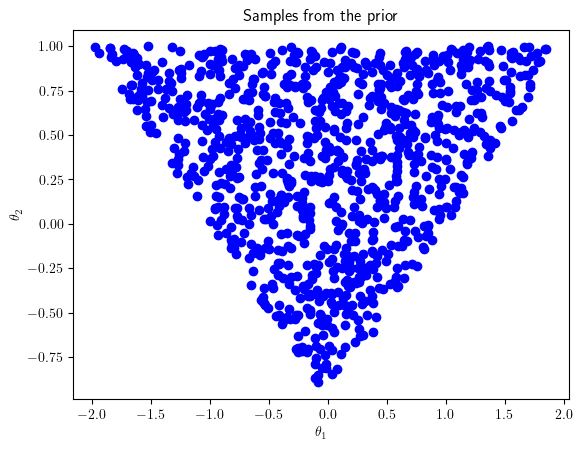
\includegraphics[width=0.48\textwidth]{./latex_files/images/chapter4/mae2_prior_samples.png}
%     \end{center}
%     \caption[MA2 example, prior distribution.]{Prior distribution proposed by \cite{Marin2012}. The
%       samples follow a triangular shape.}
%   \label{fig:ma2_1}
% \end{figure}

\noindent
The observation vector \(\yb_0 = (y_1, \ldots, y_{100})\) is generated
with \(\thetab^*=(0.6, 0.2)\). The dimensionality of the output
\(\yb\) is high, therefore we use summary statistics. Considering that
the ouptput vector represents a time-series signal, we select the
autocovariances with \(\mathrm{lag}=1\) and \(\mathrm{lag}=2\), as shown in equations
\eqref{eq:ma2_summary_1} and \eqref{eq:ma2_summary_2}. The final
distance node is the squared Euclidean distance
\eqref{eq:ma2_summary_4}.

\begin{gather} \label{eq:ma2_summary_1}
  s_1(\yb) = \frac{1}{T-1} \sum_{t=2}^T y_ty_{t-1}\\ \label{eq:ma2_summary_2}
  s_2(\yb) = \frac{1}{T-2} \sum_{t=3}^T y_ty_{t-2} \\
  s(\yb) = (s_1(\yb), s_2(\yb))\\ \label{eq:ma2_summary_4}
  d = ||s(\yb) - s(\yb_0)||_2^2 
\end{gather}

\subsubsection*{Inference}

In order to show all the capabilities of the implementation, we
perform the inference (i) using the gradient-based optimizer, (ii)
using the Bayesian Optimisation scheme and (iii) fitting a Neural
Network (NN) as a surrogate model. We use the Rejection ABC algorithm
for evaluating all approaches. Replacing the typical quadratic
surrogate model with a NN serves as an illustrator of the
extensibility of our implementation. The replacement is done by coding
a custom optimisation function with a surrogate model of our own
preference, as shown in Chapter~\ref{subsec:extensibility}. For the
definition of the NN, we use the \pkg{MLPRegressor} class of the
\pkg{scikit-learn} package. Therefore, the NN substitutes the real
distance function \(d_i\) inside the proposal region
\(q_i~ \forall i\) at the inference phase i.e.~sampling,
computing an expectation and evaluating the posterior. In our example
we use a neural network of two hidden layers of 10 neurons each and we
train it sampling 500 examples from each proposal region.

In Figure \ref{fig:ma2_5}, we illustrate the acceptance region of the
same deterministic simulator, in the gradient-based and the Bayesian
optimisation case. The acceptance regions are quite similar even though the
different optimisation schemes lead to different optimal points.

In Figure \ref{fig:ma2_3}, we demonstrate the histograms of the
marginal posteriors, for each approach; (a) Rejection ABC (first
column), (b) ROMC with gradient-based optimisation (second column) (c)
ROMC with Bayesian optimisation (third column) and (d) ROMC with the
NN extension. We observe a significant agreement between the
different approaches. At Table \ref{tab:ma2} we present the empirical
mean \(\mu\) and standard deviation \(\sigma\) for each inference
approach and finally, in Figure \ref{fig:ma2_4}, we illustrate the
unnormalised posterior for the three different variations of the ROMC
method. The results show that all ROMC variations provide consistent
results between them and in comparison with the standard Rejection ABC
algorithm.

\begin{table}
\begin{center}
\begin{tabular}{ c|c|c|c|c }
\hline
& \(\mu_{\theta_1}\) & \(\sigma_{\theta_1}\) & \(\mu_{\theta_2}\) & \(\sigma_{\theta_2}\) \\
\hline \hline
Rejection ABC & 0.516 & 0.142 & 0.07 & 0.172 \\
\hline
ROMC (gradient-based) & 0.503 & 0.143 & 0.032 & 0.17 \\
\hline
ROMC (Bayesian optimisation) & 0.494 & 0.16 & 0.086 & 0.167 \\
\hline
ROMC (Neural Network) & 0.503 & 0.140 & 0.03 & 0.171 \\
\hline
\end{tabular}
\end{center}
\caption{Comparison of the samples obtained from the estimated
  posterior with (a) Rejection sampling and (b) the different versions
  of ROMC. We observe that the obtained samples share similar
  statistics along all methods. \label{tab:ma2}}
\end{table}

\begin{figure}[ht]
    \begin{center}
        % % This file was created by tikzplotlib v0.9.9.
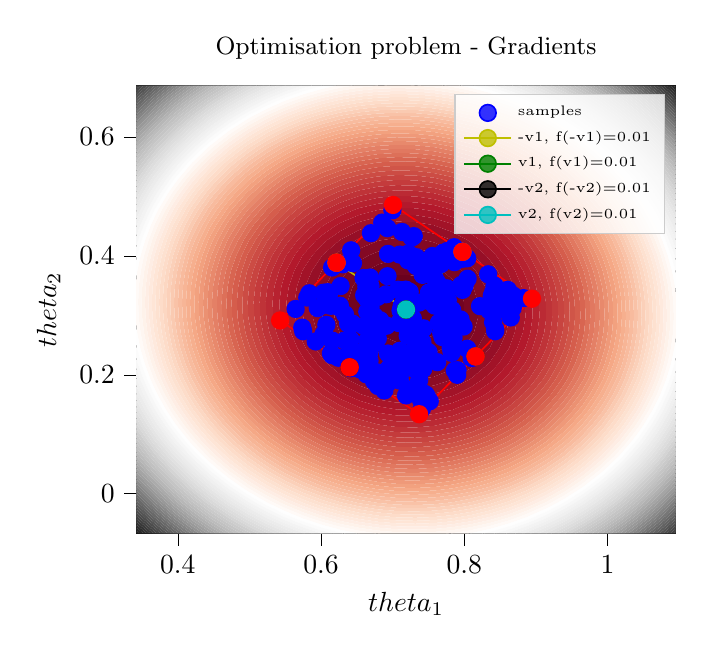
\begin{tikzpicture}

\definecolor{color0}{rgb}{0.415455594002307,0.00369088811995386,0.123414071510957}
\definecolor{color1}{rgb}{0.450057670126874,0.0147635524798155,0.128950403690888}
\definecolor{color2}{rgb}{0.484659746251442,0.025836216839677,0.134486735870819}
\definecolor{color3}{rgb}{0.519261822376009,0.0369088811995386,0.14002306805075}
\definecolor{color4}{rgb}{0.553863898500577,0.0479815455594002,0.145559400230681}
\definecolor{color5}{rgb}{0.588465974625144,0.0590542099192618,0.151095732410611}
\definecolor{color6}{rgb}{0.634602076124567,0.0738177623990773,0.158477508650519}
\definecolor{color7}{rgb}{0.669204152249135,0.0848904267589389,0.16401384083045}
\definecolor{color8}{rgb}{0.70080738177624,0.0996539792387543,0.171241830065359}
\definecolor{color9}{rgb}{0.717416378316032,0.132871972318339,0.186928104575163}
\definecolor{color10}{rgb}{0.734025374855825,0.166089965397924,0.202614379084967}
\definecolor{color11}{rgb}{0.750634371395617,0.199307958477509,0.218300653594771}
\definecolor{color12}{rgb}{0.767243367935409,0.232525951557093,0.233986928104575}
\definecolor{color13}{rgb}{0.783852364475202,0.265743944636678,0.249673202614379}
\definecolor{color14}{rgb}{0.800461361014994,0.298961937716263,0.265359477124183}
\definecolor{color15}{rgb}{0.817070357554787,0.332179930795848,0.281045751633987}
\definecolor{color16}{rgb}{0.833679354094579,0.365397923875433,0.296732026143791}
\definecolor{color17}{rgb}{0.848442906574394,0.397693194925029,0.318262206843522}
\definecolor{color18}{rgb}{0.866897347174164,0.440138408304498,0.350865051903114}
\definecolor{color19}{rgb}{0.880738177623991,0.4719723183391,0.375317185697808}
\definecolor{color20}{rgb}{0.894579008073818,0.503806228373702,0.399769319492503}
\definecolor{color21}{rgb}{0.908419838523645,0.535640138408304,0.424221453287197}
\definecolor{color22}{rgb}{0.922260668973472,0.567474048442906,0.448673587081891}
\definecolor{color23}{rgb}{0.936101499423299,0.599307958477509,0.473125720876586}
\definecolor{color24}{rgb}{0.949942329873126,0.631141868512111,0.49757785467128}
\definecolor{color25}{rgb}{0.958938869665513,0.659515570934256,0.525720876585928}
\definecolor{color26}{rgb}{0.963091118800461,0.684429065743945,0.55755478662053}
\definecolor{color27}{rgb}{0.967243367935409,0.709342560553633,0.589388696655132}
\definecolor{color28}{rgb}{0.971395617070358,0.734256055363322,0.621222606689735}
\definecolor{color29}{rgb}{0.975547866205306,0.75916955017301,0.653056516724337}
\definecolor{color30}{rgb}{0.981084198385237,0.792387543252595,0.695501730103806}
\definecolor{color31}{rgb}{0.985236447520185,0.817301038062284,0.727335640138408}
\definecolor{color32}{rgb}{0.989388696655133,0.842214532871972,0.75916955017301}
\definecolor{color33}{rgb}{0.992464436755094,0.864359861591695,0.789004229142637}
\definecolor{color34}{rgb}{0.993387158785083,0.880968858131488,0.814840445982314}
\definecolor{color35}{rgb}{0.994309880815071,0.89757785467128,0.840676662821991}
\definecolor{color36}{rgb}{0.99523260284506,0.914186851211073,0.866512879661669}
\definecolor{color37}{rgb}{0.996155324875048,0.930795847750865,0.892349096501346}
\definecolor{color38}{rgb}{0.997078046905037,0.947404844290657,0.918185313341023}
\definecolor{color39}{rgb}{0.998000768935025,0.96401384083045,0.9440215301807}
\definecolor{color40}{rgb}{0.998923490965013,0.980622837370242,0.969857747020377}
\definecolor{color41}{rgb}{0.75,0.75,0}
\definecolor{color42}{rgb}{0,0.75,0.75}

\begin{axis}[
legend cell align={left},
legend style={fill opacity=0.8, draw opacity=1, text opacity=1, draw=white!80!black, font=\tiny},
tick align=outside,
tick pos=left,
title={\small{Optimisation problem - Gradients}},
x grid style={white!69.0196078431373!black},
xlabel={$theta_1$},
xmin=0.341920057614702, xmax=1.09547344820798,
xtick style={color=black},
y grid style={white!69.0196078431373!black},
ylabel={$theta_2$},
ymin=-0.0671750541267862, ymax=0.686378336466488,
ytick style={color=black}
]
\addplot [draw=none, fill=color0, forget plot]
table{%
x  y
0.679719853397894 0.268305875054044
0.705704453073524 0.254648665147049
0.731689052749154 0.253866333404131
0.757673652424784 0.266521669054969
0.761718294504052 0.270624741656406
0.77429601761817 0.296609341332036
0.77408180687093 0.322593941007666
0.761604093021232 0.348578540683296
0.757673652424784 0.352743549667271
0.731689052749154 0.367068895692352
0.705704453073524 0.367939840933464
0.679719853397894 0.354740456073935
0.673916852624534 0.348578540683296
0.662498138024631 0.322593941007666
0.663845559392004 0.296609341332036
0.677431484005422 0.270624741656406
0.679719853397894 0.268305875054044
};
\addplot [draw=none, fill=color1, forget plot]
table{%
x  y
0.679719853397894 0.238042247186141
0.705704453073524 0.228560084919099
0.731689052749154 0.227784856113634
0.757673652424784 0.2359703542983
0.770676838975704 0.244640141980775
0.783658252100414 0.257811862729106
0.791897395341432 0.270624741656406
0.799979285903208 0.296609341332036
0.799596492681741 0.322593941007666
0.79098376739236 0.348578540683296
0.783658252100414 0.359975144104141
0.769880675178632 0.374563140358926
0.757673652424784 0.383303484618266
0.731689052749154 0.393104636929121
0.705704453073524 0.393937598664964
0.679719853397894 0.385532846865112
0.663753933811605 0.374563140358926
0.653735253722264 0.363915204358777
0.644321761275156 0.348578540683296
0.637006714152278 0.322593941007666
0.638144946367618 0.296609341332036
0.647501942617311 0.270624741656406
0.653735253722264 0.261344192131611
0.670222601461731 0.244640141980775
0.679719853397894 0.238042247186141

0.677431484005422 0.270624741656406
0.663845559392004 0.296609341332036
0.662498138024631 0.322593941007666
0.673916852624534 0.348578540683296
0.679719853397894 0.354740456073935
0.705704453073524 0.367939840933464
0.731689052749154 0.367068895692352
0.757673652424784 0.352743549667271
0.761604093021232 0.348578540683296
0.77408180687093 0.322593941007666
0.77429601761817 0.296609341332036
0.761718294504052 0.270624741656406
0.757673652424784 0.266521669054969
0.731689052749154 0.253866333404131
0.705704453073524 0.254648665147049
0.679719853397894 0.268305875054044
0.677431484005422 0.270624741656406
};
\addplot [draw=none, fill=color2, forget plot]
table{%
x  y
0.679719853397894 0.216226479230931
0.705704453073524 0.208923253385736
0.731689052749154 0.208198283036773
0.757673652424784 0.214195394809912
0.766723737407456 0.218655542305145
0.783658252100414 0.22989114527578
0.798088321840012 0.244640141980775
0.809642851776045 0.262705118742658
0.813392623346641 0.270624741656406
0.819295508245036 0.296609341332036
0.818872727900617 0.322593941007666
0.812256318269031 0.348578540683296
0.809642851776045 0.353904094293948
0.796296021537083 0.374563140358926
0.783658252100414 0.387852274800903
0.765994869195438 0.400547740034556
0.757673652424784 0.405076446007768
0.731689052749154 0.412568383227522
0.705704453073524 0.413334000766452
0.679719853397894 0.40722283700308
0.666474059091231 0.400547740034556
0.653735253722264 0.391835625662341
0.63734421445974 0.374563140358926
0.627750654046634 0.358838091691638
0.623117660442528 0.348578540683296
0.617787718558082 0.322593941007666
0.618777044490189 0.296609341332036
0.625953701998208 0.270624741656406
0.627750654046634 0.26711801992044
0.642915619681069 0.244640141980775
0.653735253722264 0.233596287766641
0.675153484298464 0.218655542305145
0.679719853397894 0.216226479230931

0.670222601461731 0.244640141980775
0.653735253722264 0.261344192131611
0.647501942617311 0.270624741656406
0.638144946367618 0.296609341332036
0.637006714152278 0.322593941007666
0.644321761275156 0.348578540683296
0.653735253722264 0.363915204358777
0.663753933811605 0.374563140358926
0.679719853397894 0.385532846865112
0.705704453073524 0.393937598664964
0.731689052749154 0.393104636929121
0.757673652424784 0.383303484618266
0.769880675178632 0.374563140358926
0.783658252100414 0.359975144104141
0.79098376739236 0.348578540683296
0.799596492681741 0.322593941007666
0.799979285903208 0.296609341332036
0.791897395341432 0.270624741656406
0.783658252100414 0.257811862729106
0.770676838975704 0.244640141980775
0.757673652424784 0.2359703542983
0.731689052749154 0.227784856113634
0.705704453073524 0.228560084919099
0.679719853397894 0.238042247186141
0.670222601461731 0.244640141980775
};
\addplot [draw=none, fill=color3, forget plot]
table{%
x  y
0.705704453073524 0.191912842774273
0.731689052749154 0.191233375150407
0.739670453979259 0.192670942629515
0.757673652424784 0.196747584143872
0.783658252100415 0.209486735398849
0.795763068085507 0.218655542305145
0.809642851776045 0.232845130423102
0.818162168453697 0.244640141980775
0.830404780679452 0.270624741656406
0.835627451451675 0.294076097598616
0.836075289949995 0.296609341332036
0.835642698277363 0.322593941007666
0.835627451451675 0.322666928771629
0.8289133799139 0.348578540683296
0.816116633883937 0.374563140358926
0.809642851776045 0.383501302922123
0.793424359603336 0.400547740034556
0.783658252100414 0.408338221551002
0.757673652424784 0.422536794588137
0.744001588121413 0.426532339710186
0.731689052749154 0.429427611775722
0.705704453073524 0.430137774099928
0.686023235059441 0.426532339710186
0.679719853397894 0.425073757617429
0.653735253722264 0.412064932476403
0.638870636039256 0.400547740034556
0.627750654046634 0.388823655887986
0.617764154518083 0.374563140358926
0.6061010483075 0.348578540683296
0.601766054371004 0.326983114398766
0.601066686366283 0.322593941007666
0.601766054371004 0.302102740256347
0.601998945440227 0.296609341332036
0.609292369604236 0.270624741656406
0.622643222508885 0.244640141980775
0.627750654046634 0.237792663993768
0.646502768036196 0.218655542305145
0.653735253722264 0.213014626922426
0.679719853397894 0.199151984405328
0.702418888492385 0.192670942629515
0.705704453073524 0.191912842774273

0.675153484298464 0.218655542305145
0.653735253722264 0.233596287766641
0.642915619681069 0.244640141980775
0.627750654046634 0.26711801992044
0.625953701998208 0.270624741656406
0.618777044490189 0.296609341332036
0.617787718558082 0.322593941007666
0.623117660442528 0.348578540683296
0.627750654046634 0.358838091691638
0.63734421445974 0.374563140358926
0.653735253722264 0.391835625662341
0.666474059091231 0.400547740034556
0.679719853397894 0.40722283700308
0.705704453073524 0.413334000766452
0.731689052749154 0.412568383227522
0.757673652424784 0.405076446007768
0.765994869195438 0.400547740034556
0.783658252100414 0.387852274800903
0.796296021537083 0.374563140358926
0.809642851776045 0.353904094293948
0.812256318269031 0.348578540683296
0.818872727900617 0.322593941007666
0.819295508245036 0.296609341332036
0.813392623346641 0.270624741656406
0.809642851776045 0.262705118742658
0.798088321840012 0.244640141980775
0.783658252100414 0.22989114527578
0.766723737407456 0.218655542305145
0.757673652424784 0.214195394809912
0.731689052749154 0.208198283036773
0.705704453073524 0.208923253385736
0.679719853397894 0.216226479230931
0.675153484298464 0.218655542305145
};
\addplot [draw=none, fill=color4, forget plot]
table{%
x  y
0.679719853397894 0.184159158183395
0.705704453073524 0.178114502701054
0.731689052749154 0.17735504605529
0.757673652424784 0.181973239128259
0.783658252100414 0.19206370170059
0.784671584944026 0.192670942629515
0.809642851776045 0.211540663230551
0.816577518685196 0.218655542305145
0.835296079512027 0.244640141980775
0.835627451451675 0.245345623498239
0.845039223052204 0.270624741656406
0.849579809790021 0.296609341332036
0.849071468273359 0.322593941007666
0.843598686263512 0.348578540683296
0.835627451451675 0.368556479552963
0.832658601729762 0.374563140358926
0.813809541115679 0.400547740034556
0.809642851776045 0.404912479160995
0.783658252100414 0.425672149990662
0.782087232477782 0.426532339710186
0.757673652424784 0.437303408472928
0.731689052749154 0.443476852422172
0.705704453073524 0.444269947900272
0.679719853397894 0.439586847969589
0.653735253722264 0.429329415503186
0.649150806650493 0.426532339710186
0.627750654046634 0.409987854311522
0.618758110225292 0.400547740034556
0.601766054371004 0.376208325685115
0.600857068176069 0.374563140358926
0.591642611738036 0.348578540683296
0.58755935951281 0.322593941007666
0.588520947469287 0.296609341332036
0.594442938903781 0.270624741656406
0.601766054371004 0.253036776317643
0.606097042735943 0.244640141980775
0.625494162900175 0.218655542305145
0.627750654046634 0.216343882340804
0.653735253722264 0.196061045841453
0.660068807473501 0.192670942629515
0.679719853397894 0.184159158183395

0.702418888492385 0.192670942629515
0.679719853397894 0.199151984405328
0.653735253722264 0.213014626922426
0.646502768036196 0.218655542305145
0.627750654046634 0.237792663993768
0.622643222508885 0.244640141980775
0.609292369604236 0.270624741656406
0.601998945440226 0.296609341332036
0.601766054371004 0.302102740256347
0.601066686366283 0.322593941007666
0.601766054371004 0.326983114398766
0.6061010483075 0.348578540683296
0.617764154518083 0.374563140358926
0.627750654046634 0.388823655887986
0.638870636039256 0.400547740034556
0.653735253722264 0.412064932476403
0.679719853397894 0.425073757617429
0.686023235059441 0.426532339710186
0.705704453073524 0.430137774099928
0.731689052749154 0.429427611775722
0.744001588121413 0.426532339710186
0.757673652424784 0.422536794588137
0.783658252100414 0.408338221551002
0.793424359603336 0.400547740034556
0.809642851776045 0.383501302922123
0.816116633883937 0.374563140358926
0.8289133799139 0.348578540683296
0.835627451451675 0.322666928771629
0.835642698277363 0.322593941007666
0.836075289949995 0.296609341332036
0.835627451451675 0.294076097598616
0.830404780679452 0.270624741656406
0.818162168453697 0.244640141980775
0.809642851776045 0.232845130423102
0.795763068085507 0.218655542305145
0.783658252100415 0.209486735398849
0.757673652424784 0.196747584143872
0.739670453979259 0.192670942629515
0.731689052749154 0.191233375150407
0.705704453073524 0.191912842774273
0.702418888492385 0.192670942629515
};
\addplot [draw=none, fill=color5, forget plot]
table{%
x  y
0.705704453073524 0.164707296888947
0.731689052749154 0.1640089403686
0.750101563557335 0.166686342953885
0.757673652424784 0.168013988210559
0.783658252100414 0.178022579746989
0.808102696647773 0.192670942629515
0.809642851776045 0.193834772127964
0.83383493878171 0.218655542305145
0.835627451451675 0.221144177469267
0.84902190475963 0.244640141980775
0.858620352173124 0.270624741656406
0.861612051127305 0.288006756967876
0.862838394647627 0.296609341332036
0.862352565973855 0.322593941007666
0.861612051127305 0.326734579752303
0.856952551470694 0.348578540683296
0.84652386832075 0.374563140358926
0.835627451451675 0.393126061201861
0.830237994754614 0.400547740034556
0.809642851776045 0.422121804968578
0.804123888839356 0.426532339710186
0.783658252100414 0.439729499789758
0.757673652424784 0.451270683655426
0.752472481071863 0.452516939385816
0.731689052749154 0.456686954645117
0.705704453073524 0.457411390051119
0.679719853397894 0.453585382095002
0.676417772746349 0.452516939385816
0.653735253722264 0.443630428047781
0.627750654046634 0.42778410823127
0.626237827407337 0.426532339710186
0.601766054371004 0.400833285513834
0.601551185826641 0.400547740034556
0.587195584183223 0.374563140358926
0.578058643662388 0.348578540683296
0.575781454695373 0.333846070644159
0.574340971887777 0.322593941007666
0.575204484189329 0.296609341332036
0.575781454695373 0.293625494920339
0.581086328969514 0.270624741656406
0.591960265205223 0.244640141980775
0.601766054371004 0.228413721513765
0.609061554949172 0.218655542305145
0.627750654046634 0.199509514534991
0.63650135078467 0.192670942629515
0.653735253722264 0.181757572076383
0.679719853397894 0.170439890367809
0.695682555194535 0.166686342953885
0.705704453073524 0.164707296888947

0.660068807473501 0.192670942629515
0.653735253722264 0.196061045841453
0.627750654046634 0.216343882340804
0.625494162900175 0.218655542305145
0.606097042735943 0.244640141980775
0.601766054371004 0.253036776317643
0.594442938903781 0.270624741656406
0.588520947469287 0.296609341332036
0.58755935951281 0.322593941007666
0.591642611738036 0.348578540683296
0.600857068176069 0.374563140358926
0.601766054371004 0.376208325685115
0.618758110225292 0.400547740034556
0.627750654046634 0.409987854311522
0.649150806650493 0.426532339710186
0.653735253722264 0.429329415503186
0.679719853397894 0.439586847969589
0.705704453073524 0.444269947900272
0.731689052749154 0.443476852422172
0.757673652424784 0.437303408472928
0.782087232477782 0.426532339710186
0.783658252100414 0.425672149990662
0.809642851776045 0.404912479160995
0.813809541115679 0.400547740034556
0.832658601729762 0.374563140358926
0.835627451451675 0.368556479552963
0.843598686263512 0.348578540683296
0.849071468273359 0.322593941007666
0.849579809790021 0.296609341332036
0.845039223052204 0.270624741656406
0.835627451451675 0.245345623498239
0.835296079512027 0.244640141980775
0.816577518685197 0.218655542305145
0.809642851776045 0.211540663230551
0.784671584944026 0.192670942629515
0.783658252100414 0.19206370170059
0.757673652424784 0.181973239128259
0.731689052749154 0.17735504605529
0.705704453073524 0.178114502701054
0.679719853397894 0.184159158183395
0.660068807473501 0.192670942629515
};
\addplot [draw=none, fill=color6, forget plot]
table{%
x  y
0.679719853397894 0.158357319054258
0.705704453073524 0.153186000249851
0.731689052749154 0.152431929753816
0.757673652424784 0.156159500926373
0.783658252100414 0.16443436484953
0.788216641124798 0.166686342953885
0.809642851776045 0.17947536842405
0.825882987208455 0.192670942629515
0.835627451451675 0.202670524431201
0.847937588354553 0.218655542305145
0.861612051127305 0.242746938392896
0.862500343540992 0.244640141980775
0.870424232167654 0.270624741656406
0.874087068298725 0.296609341332036
0.873548633876836 0.322593941007666
0.868867597740976 0.348578540683296
0.861612051127305 0.370068406560432
0.85980365973179 0.374563140358926
0.844501500165251 0.400547740034556
0.835627451451675 0.412028908312598
0.821777627239647 0.426532339710186
0.809642851776045 0.436800168897473
0.785347069694985 0.452516939385816
0.783658252100414 0.453433465904882
0.757673652424784 0.463117281142027
0.731689052749154 0.468382652478943
0.705704453073524 0.469164505546848
0.679719853397894 0.465396481794743
0.653735253722264 0.457010906654679
0.644773062553913 0.452516939385816
0.627750654046634 0.442171062091677
0.608850453710227 0.426532339710186
0.601766054371004 0.419092651449879
0.587811296161487 0.400547740034556
0.575781454695373 0.378673103236628
0.573913134269825 0.374563140358926
0.566372649174092 0.348578540683296
0.563090350753328 0.322593941007666
0.564006486977237 0.296609341332036
0.569062418553035 0.270624741656406
0.575781454695373 0.251542533681821
0.578677759435704 0.244640141980775
0.594421264314578 0.218655542305145
0.601766054371004 0.209360403392822
0.61805992882883 0.192670942629515
0.627750654046634 0.184617115447215
0.653735253722264 0.168116475425088
0.657012543900356 0.166686342953885
0.679719853397894 0.158357319054258

0.695682555194535 0.166686342953885
0.679719853397894 0.170439890367809
0.653735253722264 0.181757572076383
0.63650135078467 0.192670942629515
0.627750654046634 0.199509514534991
0.609061554949172 0.218655542305145
0.601766054371004 0.228413721513765
0.591960265205223 0.244640141980775
0.581086328969514 0.270624741656406
0.575781454695373 0.29362549492034
0.575204484189329 0.296609341332036
0.574340971887777 0.322593941007666
0.575781454695373 0.333846070644159
0.578058643662388 0.348578540683296
0.587195584183223 0.374563140358926
0.601551185826641 0.400547740034556
0.601766054371004 0.400833285513834
0.626237827407337 0.426532339710186
0.627750654046634 0.42778410823127
0.653735253722264 0.443630428047781
0.676417772746349 0.452516939385816
0.679719853397894 0.453585382095002
0.705704453073524 0.457411390051119
0.731689052749154 0.456686954645117
0.752472481071863 0.452516939385816
0.757673652424784 0.451270683655426
0.783658252100414 0.439729499789758
0.804123888839356 0.426532339710186
0.809642851776044 0.422121804968578
0.830237994754614 0.400547740034556
0.835627451451675 0.393126061201861
0.84652386832075 0.374563140358926
0.856952551470694 0.348578540683296
0.861612051127305 0.326734579752303
0.862352565973855 0.322593941007666
0.862838394647627 0.296609341332036
0.861612051127305 0.288006756967876
0.858620352173124 0.270624741656406
0.84902190475963 0.244640141980775
0.835627451451675 0.221144177469267
0.83383493878171 0.218655542305145
0.809642851776045 0.193834772127964
0.808102696647773 0.192670942629515
0.783658252100414 0.178022579746989
0.757673652424784 0.168013988210559
0.750101563557335 0.166686342953885
0.731689052749154 0.1640089403686
0.705704453073524 0.164707296888947
0.695682555194535 0.166686342953885
};
\addplot [draw=none, fill=color7, forget plot]
table{%
x  y
0.653735253722264 0.15647125847213
0.679719853397894 0.146891202715861
0.705704453073524 0.141664703610755
0.731689052749154 0.140854919139032
0.757673652424784 0.144526234881152
0.783658252100414 0.152744293987412
0.809642851776045 0.165576028031938
0.811297805377675 0.166686342953885
0.835627451451674 0.18642780731369
0.841698547715321 0.192670942629515
0.861612051127305 0.218573745966965
0.861663980225797 0.218655542305145
0.873855725794389 0.244640141980775
0.88172600824639 0.270624741656406
0.885335741949821 0.296609341332036
0.884744701779817 0.322593941007666
0.880011549639459 0.348578540683296
0.871193860243349 0.374563140358926
0.861612051127305 0.393922648677839
0.85770803502057 0.400547740034556
0.83761301050649 0.426532339710186
0.835627451451675 0.428607536563756
0.809642851776045 0.450606349255428
0.80668936451296 0.452516939385816
0.783658252100415 0.465015995149765
0.757673652424784 0.474756119593217
0.739361104474176 0.478501539061447
0.731689052749154 0.479852102566667
0.705704453073524 0.480569494393681
0.688753527971025 0.478501539061447
0.679719853397894 0.477207581494484
0.653735253722264 0.468880565527251
0.627750654046634 0.455867558364166
0.622831075566489 0.452516939385816
0.601766054371004 0.435108941155809
0.593577418704557 0.426532339710186
0.575781454695373 0.402837741951858
0.57436119437701 0.400547740034556
0.562555767405632 0.374563140358926
0.555068907179744 0.348578540683296
0.551839729618879 0.322593941007666
0.552808489765144 0.296609341332036
0.557916555266454 0.270624741656406
0.567106380597053 0.244640141980775
0.575781454695373 0.227609623717277
0.581212044968145 0.218655542305145
0.601744554889927 0.192670942629515
0.601766054371004 0.192648869261882
0.627750654046634 0.171053304182649
0.634624208376609 0.166686342953885
0.653735253722264 0.15647125847213

0.657012543900356 0.166686342953885
0.653735253722264 0.168116475425088
0.627750654046634 0.184617115447215
0.61805992882883 0.192670942629515
0.601766054371004 0.209360403392822
0.594421264314578 0.218655542305145
0.578677759435705 0.244640141980775
0.575781454695373 0.251542533681821
0.569062418553035 0.270624741656406
0.564006486977237 0.296609341332036
0.563090350753328 0.322593941007666
0.566372649174092 0.348578540683296
0.573913134269825 0.374563140358926
0.575781454695373 0.378673103236628
0.587811296161487 0.400547740034556
0.601766054371004 0.419092651449879
0.608850453710227 0.426532339710186
0.627750654046634 0.442171062091677
0.644773062553913 0.452516939385816
0.653735253722264 0.457010906654679
0.679719853397894 0.465396481794743
0.705704453073524 0.469164505546848
0.731689052749154 0.468382652478943
0.757673652424784 0.463117281142027
0.783658252100414 0.453433465904882
0.785347069694985 0.452516939385816
0.809642851776045 0.436800168897473
0.821777627239647 0.426532339710186
0.835627451451675 0.412028908312598
0.844501500165251 0.400547740034556
0.85980365973179 0.374563140358926
0.861612051127305 0.370068406560432
0.868867597740976 0.348578540683296
0.873548633876836 0.322593941007666
0.874087068298724 0.296609341332036
0.870424232167654 0.270624741656406
0.862500343540992 0.244640141980775
0.861612051127305 0.242746938392896
0.847937588354553 0.218655542305145
0.835627451451675 0.202670524431201
0.825882987208455 0.192670942629515
0.809642851776045 0.17947536842405
0.788216641124798 0.166686342953885
0.783658252100414 0.16443436484953
0.757673652424784 0.156159500926373
0.731689052749154 0.152431929753816
0.705704453073524 0.153186000249851
0.679719853397894 0.158357319054258
0.657012543900356 0.166686342953885
};
\addplot [draw=none, fill=color8, forget plot]
table{%
x  y
0.679719853397894 0.136169438693335
0.705704453073524 0.131638972558086
0.731689052749154 0.130902782113927
0.757673652424784 0.13400827913659
0.782541211181572 0.140701743278255
0.783658252100414 0.141054223125295
0.809642851776045 0.153828594879071
0.828807663546713 0.166686342953885
0.835627451451675 0.172220028049745
0.855514810096403 0.192670942629515
0.861612051127305 0.200602024973843
0.873073479603099 0.218655542305145
0.885211108047785 0.244640141980775
0.887596650802935 0.252544237766403
0.892247261350541 0.270624741656406
0.895297959757871 0.296609341332036
0.894751230693004 0.322593941007666
0.890650177487299 0.348578540683296
0.887596650802935 0.358975985693347
0.882286179073593 0.374563140358926
0.869389308204177 0.400547740034556
0.861612051127305 0.412497969638119
0.850747092596051 0.426532339710186
0.835627451451675 0.442334555037819
0.823606189554594 0.452516939385816
0.809642851776045 0.462448552405196
0.783658252100414 0.476598524394648
0.778590837358409 0.478501539061447
0.757673652424784 0.485267095279482
0.731689052749154 0.489869650734974
0.705704453073524 0.490629135601878
0.679719853397894 0.487496900513874
0.653735253722264 0.480423471489692
0.649205981047231 0.478501539061447
0.627750654046634 0.46779635997305
0.605316498090455 0.452516939385816
0.601766054371004 0.449582875498086
0.57975821820417 0.426532339710186
0.575781454695373 0.421237441851756
0.562949691425777 0.400547740034556
0.55119840054144 0.374563140358926
0.549796855019743 0.369682500702179
0.544632124851833 0.348578540683296
0.541907246731734 0.322593941007666
0.542777714194302 0.296609341332036
0.547200442513339 0.270624741656406
0.549796855019743 0.262142526200469
0.556012168051183 0.244640141980775
0.569278443687901 0.218655542305145
0.575781454695373 0.208879623753346
0.588607817686351 0.192670942629515
0.601766054371004 0.179161472577126
0.616759520659885 0.166686342953885
0.627750654046634 0.158985584996035
0.653735253722264 0.14505979639087
0.665519589821022 0.140701743278255
0.679719853397894 0.136169438693335

0.634624208376609 0.166686342953885
0.627750654046634 0.171053304182649
0.601766054371004 0.192648869261882
0.601744554889927 0.192670942629515
0.581212044968145 0.218655542305145
0.575781454695373 0.227609623717277
0.567106380597053 0.244640141980775
0.557916555266454 0.270624741656406
0.552808489765144 0.296609341332036
0.551839729618879 0.322593941007666
0.555068907179744 0.348578540683296
0.562555767405632 0.374563140358926
0.57436119437701 0.400547740034556
0.575781454695373 0.402837741951858
0.593577418704557 0.426532339710186
0.601766054371004 0.435108941155809
0.622831075566489 0.452516939385816
0.627750654046634 0.455867558364166
0.653735253722264 0.468880565527251
0.679719853397894 0.477207581494484
0.688753527971025 0.478501539061447
0.705704453073524 0.480569494393681
0.731689052749154 0.479852102566667
0.739361104474176 0.478501539061447
0.757673652424784 0.474756119593218
0.783658252100414 0.465015995149765
0.80668936451296 0.452516939385816
0.809642851776045 0.450606349255428
0.835627451451675 0.428607536563756
0.83761301050649 0.426532339710186
0.85770803502057 0.400547740034556
0.861612051127305 0.393922648677839
0.871193860243349 0.374563140358926
0.880011549639459 0.348578540683296
0.884744701779817 0.322593941007666
0.885335741949821 0.296609341332036
0.88172600824639 0.270624741656406
0.873855725794389 0.244640141980775
0.861663980225797 0.218655542305145
0.861612051127305 0.218573745966965
0.841698547715321 0.192670942629515
0.835627451451675 0.18642780731369
0.811297805377675 0.166686342953885
0.809642851776045 0.165576028031938
0.783658252100414 0.152744293987412
0.757673652424784 0.144526234881152
0.731689052749154 0.140854919139032
0.705704453073524 0.141664703610755
0.679719853397894 0.146891202715861
0.653735253722264 0.15647125847213
0.634624208376609 0.166686342953885
};
\addplot [draw=none, fill=color9, forget plot]
table{%
x  y
0.653735253722264 0.134639247976646
0.679719853397894 0.126320791599385
0.705704453073524 0.121749642761502
0.731689052749154 0.120972432117093
0.757673652424784 0.124036567224655
0.783658252100414 0.130990248794581
0.806836569747568 0.140701743278255
0.809642851776045 0.142081161726204
0.835627451451675 0.159478966450791
0.844111479801476 0.166686342953885
0.861612051127305 0.184685795548344
0.868016959978152 0.192670942629515
0.884482978980401 0.218655542305145
0.887596650802935 0.225327634043733
0.895272178217223 0.244640141980775
0.901924828441038 0.270624741656406
0.90493656435729 0.296609341332036
0.904351185274169 0.322593941007666
0.900211790779072 0.348578540683296
0.89256079465611 0.374563140358926
0.887596650802935 0.386136695035053
0.880430470220659 0.400547740034556
0.863510832126102 0.426532339710186
0.861612051127305 0.428890382004849
0.839000470846641 0.452516939385816
0.835627451451675 0.455479154073728
0.809642851776045 0.473975314673218
0.801336402781257 0.478501539061447
0.783658252100414 0.486803721205502
0.757673652424784 0.495242901203904
0.731689052749154 0.499887198903281
0.705704453073524 0.500688776810075
0.679719853397894 0.497598989998686
0.653735253722264 0.490568369003837
0.627750654046634 0.479546602276118
0.625940818007862 0.478501539061447
0.601766054371004 0.462075236176666
0.590684226588223 0.452516939385816
0.575781454695373 0.436903800870695
0.567614923374092 0.426532339710186
0.551538188474543 0.400547740034556
0.549796855019743 0.396695091740115
0.541277833852229 0.374563140358926
0.534953116333186 0.348578540683296
0.532267212288217 0.322593941007666
0.533176341214008 0.296609341332036
0.53763742213054 0.270624741656406
0.54560805966548 0.244640141980775
0.549796855019743 0.235148453947655
0.558235405384296 0.218655542305145
0.57552174507678 0.192670942629515
0.575781454695373 0.192354068760447
0.600785485903448 0.166686342953885
0.601766054371004 0.165837968329298
0.627750654046634 0.147628258614962
0.64065591374097 0.140701743278255
0.653735253722264 0.134639247976646

0.665519589821022 0.140701743278255
0.653735253722264 0.14505979639087
0.627750654046634 0.158985584996035
0.616759520659885 0.166686342953885
0.601766054371004 0.179161472577126
0.588607817686351 0.192670942629515
0.575781454695373 0.208879623753346
0.569278443687901 0.218655542305145
0.556012168051183 0.244640141980775
0.549796855019743 0.262142526200469
0.547200442513339 0.270624741656406
0.542777714194302 0.296609341332036
0.541907246731734 0.322593941007666
0.544632124851833 0.348578540683296
0.549796855019743 0.369682500702179
0.55119840054144 0.374563140358926
0.562949691425777 0.400547740034556
0.575781454695373 0.421237441851756
0.57975821820417 0.426532339710186
0.601766054371004 0.449582875498086
0.605316498090454 0.452516939385816
0.627750654046634 0.46779635997305
0.649205981047231 0.478501539061447
0.653735253722264 0.480423471489692
0.679719853397894 0.487496900513874
0.705704453073524 0.490629135601878
0.731689052749154 0.489869650734974
0.757673652424784 0.485267095279482
0.778590837358409 0.478501539061447
0.783658252100414 0.476598524394648
0.809642851776045 0.462448552405196
0.823606189554594 0.452516939385816
0.835627451451675 0.442334555037819
0.850747092596051 0.426532339710186
0.861612051127305 0.412497969638119
0.869389308204177 0.400547740034556
0.882286179073593 0.374563140358926
0.887596650802935 0.358975985693347
0.890650177487299 0.348578540683296
0.894751230693004 0.322593941007666
0.895297959757871 0.296609341332036
0.892247261350541 0.270624741656406
0.887596650802935 0.252544237766403
0.885211108047785 0.244640141980775
0.873073479603099 0.218655542305145
0.861612051127305 0.200602024973843
0.855514810096403 0.192670942629515
0.835627451451675 0.172220028049745
0.828807663546713 0.166686342953885
0.809642851776045 0.153828594879071
0.783658252100414 0.141054223125295
0.782541211181572 0.140701743278255
0.757673652424784 0.13400827913659
0.731689052749154 0.130902782113927
0.705704453073524 0.131638972558086
0.679719853397894 0.136169438693335
0.665519589821022 0.140701743278255
};
\addplot [draw=none, fill=color10, forget plot]
table{%
x  y
0.705704453073524 0.112214768943233
0.731689052749154 0.111499714415033
0.757673652424784 0.114146376708996
0.760135124145806 0.114717143602625
0.783658252100414 0.120976828964899
0.809642851776045 0.131827009236201
0.825210510751535 0.140701743278255
0.835627451451675 0.147673605286408
0.85800793973461 0.166686342953885
0.861612051127305 0.170393195201744
0.879481094768783 0.192670942629515
0.887596650802935 0.205489499476491
0.894690545171169 0.218655542305145
0.904989024076361 0.244640141980775
0.911602395531534 0.270624741656406
0.913581250478565 0.287898292444471
0.914450718423827 0.296609341332036
0.913904987807337 0.322593941007666
0.913581250478565 0.324886193824375
0.909773404070845 0.348578540683296
0.902084371702971 0.374563140358926
0.890925780693171 0.400547740034556
0.887596650802935 0.406459988164733
0.874501307024217 0.426532339710186
0.861612051127305 0.442539141216468
0.852062890803498 0.452516939385816
0.835627451451675 0.466950683799766
0.819419070396158 0.478501539061447
0.809642851776045 0.484510062081852
0.783658252100414 0.496738131315031
0.759909739235374 0.504486138737077
0.757673652424784 0.505127119631743
0.731689052749154 0.509224820388964
0.705704453073524 0.509959741549741
0.679719853397894 0.507294694726962
0.667737605306756 0.504486138737077
0.653735253722264 0.500713266517982
0.627750654046634 0.489734672165177
0.608297161823345 0.478501539061447
0.601766054371004 0.474063772852157
0.576784794324044 0.452516939385816
0.575781454695373 0.451465773823277
0.556148765773297 0.426532339710186
0.549796855019743 0.416260507385311
0.541527949333172 0.400547740034556
0.53155953483954 0.374563140358926
0.525274107814538 0.348578540683296
0.523812255344113 0.334253636650883
0.522775583039157 0.322593941007666
0.523604578984765 0.296609341332036
0.523812255344113 0.295244174975176
0.528074401747741 0.270624741656406
0.536083086701003 0.244640141980775
0.547559303372236 0.218655542305145
0.549796855019743 0.214767201410426
0.564529411080548 0.192670942629515
0.575781454695373 0.178942230483753
0.587720439730079 0.166686342953885
0.601766054371004 0.154534266436684
0.621469180335981 0.140701743278255
0.627750654046634 0.136890864637137
0.653735253722264 0.124830950235843
0.679719853397894 0.116472144505436
0.689633377650254 0.114717143602625
0.705704453073524 0.112214768943233

0.64065591374097 0.140701743278255
0.627750654046634 0.147628258614962
0.601766054371004 0.165837968329298
0.600785485903448 0.166686342953885
0.575781454695373 0.192354068760447
0.57552174507678 0.192670942629515
0.558235405384296 0.218655542305145
0.549796855019743 0.235148453947655
0.54560805966548 0.244640141980775
0.53763742213054 0.270624741656406
0.533176341214008 0.296609341332036
0.532267212288217 0.322593941007666
0.534953116333186 0.348578540683296
0.541277833852229 0.374563140358926
0.549796855019743 0.396695091740115
0.551538188474543 0.400547740034556
0.567614923374092 0.426532339710186
0.575781454695373 0.436903800870695
0.590684226588223 0.452516939385816
0.601766054371004 0.462075236176666
0.625940818007862 0.478501539061447
0.627750654046634 0.479546602276118
0.653735253722264 0.490568369003836
0.679719853397894 0.497598989998686
0.705704453073524 0.500688776810075
0.731689052749154 0.499887198903281
0.757673652424784 0.495242901203904
0.783658252100414 0.486803721205502
0.801336402781257 0.478501539061447
0.809642851776045 0.473975314673218
0.835627451451675 0.455479154073728
0.839000470846641 0.452516939385816
0.861612051127305 0.428890382004849
0.863510832126102 0.426532339710186
0.880430470220659 0.400547740034556
0.887596650802935 0.386136695035053
0.89256079465611 0.374563140358926
0.900211790779072 0.348578540683296
0.904351185274169 0.322593941007666
0.90493656435729 0.296609341332036
0.901924828441038 0.270624741656406
0.895272178217223 0.244640141980775
0.887596650802935 0.225327634043733
0.884482978980401 0.218655542305145
0.868016959978152 0.192670942629515
0.861612051127305 0.184685795548344
0.844111479801476 0.166686342953885
0.835627451451675 0.159478966450791
0.809642851776045 0.142081161726204
0.806836569747568 0.140701743278255
0.783658252100414 0.130990248794581
0.757673652424784 0.124036567224655
0.731689052749154 0.120972432117093
0.705704453073524 0.121749642761502
0.679719853397894 0.126320791599385
0.653735253722264 0.134639247976646
0.64065591374097 0.140701743278255
};
\addplot [draw=none, fill=color11, forget plot]
table{%
x  y
0.679719853397894 0.107624081212213
0.705704453073524 0.103552439453095
0.731689052749154 0.102805928453591
0.757673652424784 0.105420904980888
0.783658252100414 0.111434257771099
0.79270758516212 0.114717143602625
0.809642851776045 0.121771531126293
0.835627451451675 0.13656733791381
0.84135033342083 0.140701743278255
0.861612051127305 0.157899427668999
0.870143764217111 0.166686342953885
0.887596650802935 0.188471119392695
0.890458088632223 0.192670942629515
0.904446989943275 0.218655542305145
0.913581250478565 0.241781274836372
0.914564055140452 0.244640141980775
0.920312584321924 0.270624741656406
0.922882453943928 0.296609341332036
0.922307131387659 0.322593941007666
0.918619615850219 0.348578540683296
0.913581250478565 0.367907603339109
0.911607948749832 0.374563140358926
0.900411622913609 0.400547740034556
0.887596650802935 0.423306027454283
0.885491781922332 0.426532339710186
0.864554533643331 0.452516939385816
0.861612051127305 0.455587600636536
0.835627451451675 0.478422213525805
0.835516140342671 0.478501539061447
0.809642851776045 0.494403418510657
0.788273065857305 0.504486138737077
0.783658252100414 0.506400184998535
0.757673652424784 0.51385572583813
0.731689052749154 0.517985367151446
0.705704453073524 0.518752463486772
0.679719853397894 0.516119829051599
0.653735253722264 0.510049727716559
0.638567312502411 0.504486138737077
0.627750654046634 0.499922742054236
0.601766054371004 0.484945740749521
0.592960616920977 0.478501539061447
0.575781454695373 0.463696056605185
0.56509179175284 0.452516939385816
0.549796855019743 0.43306716060996
0.545426725233632 0.426532339710186
0.531770039538459 0.400547740034556
0.523812255344113 0.379738318624383
0.522089814363666 0.374563140358926
0.516627756900225 0.348578540683296
0.514342753345431 0.322593941007666
0.515201348898039 0.296609341332036
0.51917055682522 0.270624741656406
0.523812255344113 0.2535304000095
0.526558113736526 0.244640141980775
0.53807207627503 0.218655542305145
0.549796855019743 0.198280621920451
0.553537077084315 0.192670942629515
0.574838368406786 0.166686342953885
0.575781454695373 0.165716668423566
0.601766054371004 0.143230564544069
0.605368122003393 0.140701743278255
0.627750654046634 0.127122586980417
0.653735253722264 0.11502265249504
0.654684157641145 0.114717143602625
0.679719853397894 0.107624081212213

0.689633377650254 0.114717143602625
0.679719853397894 0.116472144505436
0.653735253722264 0.124830950235843
0.627750654046634 0.136890864637137
0.621469180335981 0.140701743278255
0.601766054371004 0.154534266436684
0.587720439730079 0.166686342953885
0.575781454695373 0.178942230483753
0.564529411080548 0.192670942629515
0.549796855019743 0.214767201410426
0.547559303372236 0.218655542305145
0.536083086701003 0.244640141980775
0.528074401747741 0.270624741656406
0.523812255344113 0.295244174975176
0.523604578984765 0.296609341332036
0.522775583039157 0.322593941007666
0.523812255344113 0.334253636650883
0.525274107814538 0.348578540683296
0.53155953483954 0.374563140358926
0.541527949333172 0.400547740034556
0.549796855019743 0.416260507385311
0.556148765773297 0.426532339710186
0.575781454695373 0.451465773823277
0.576784794324044 0.452516939385816
0.601766054371004 0.474063772852157
0.608297161823345 0.478501539061447
0.627750654046634 0.489734672165177
0.653735253722264 0.500713266517981
0.667737605306756 0.504486138737077
0.679719853397894 0.507294694726962
0.705704453073524 0.509959741549741
0.731689052749154 0.509224820388964
0.757673652424784 0.505127119631743
0.759909739235374 0.504486138737077
0.783658252100414 0.496738131315031
0.809642851776045 0.484510062081852
0.819419070396158 0.478501539061447
0.835627451451675 0.466950683799766
0.852062890803498 0.452516939385816
0.861612051127305 0.442539141216468
0.874501307024217 0.426532339710186
0.887596650802935 0.406459988164733
0.890925780693171 0.400547740034556
0.902084371702971 0.374563140358926
0.909773404070845 0.348578540683296
0.913581250478565 0.324886193824375
0.913904987807337 0.322593941007666
0.914450718423827 0.296609341332036
0.913581250478565 0.287898292444471
0.911602395531534 0.270624741656406
0.904989024076361 0.244640141980775
0.894690545171169 0.218655542305145
0.887596650802935 0.205489499476491
0.879481094768783 0.192670942629515
0.861612051127305 0.170393195201744
0.85800793973461 0.166686342953885
0.835627451451675 0.147673605286408
0.825210510751535 0.140701743278255
0.809642851776045 0.131827009236201
0.783658252100414 0.120976828964899
0.760135124145806 0.114717143602625
0.757673652424784 0.114146376708996
0.731689052749154 0.111499714415033
0.705704453073524 0.112214768943233
0.689633377650254 0.114717143602625
};
\addplot [draw=none, fill=color12, forget plot]
table{%
x  y
0.653735253722264 0.106384924828473
0.679719853397894 0.0989929813779969
0.705704453073524 0.0948901099629559
0.731689052749154 0.0941121424921504
0.757673652424784 0.0966954332527799
0.783658252100414 0.102676868464688
0.809642851776045 0.112093876045066
0.814946304502179 0.114717143602625
0.835627451451675 0.12646944672781
0.855327927367431 0.140701743278255
0.861612051127305 0.146035564361951
0.881663060191948 0.166686342953885
0.887596650802935 0.174092679109462
0.90025445639168 0.192670942629515
0.913581250478565 0.217491987443696
0.914124697852795 0.218655542305145
0.923055604304318 0.244640141980775
0.928774120961261 0.270624741656406
0.93131418946403 0.296609341332036
0.930709274967981 0.322593941007666
0.926992374475518 0.348578540683296
0.920196024993953 0.374563140358926
0.913581250478565 0.392004322286447
0.909897465134046 0.400547740034556
0.895235520575905 0.426532339710186
0.887596650802935 0.437504568032311
0.875494784679284 0.452516939385816
0.861612051127305 0.467004424609584
0.848529150673643 0.478501539061447
0.835627451451675 0.488286048788791
0.809642851776045 0.504296774939461
0.80924150534126 0.504486138737077
0.783658252100414 0.515097082710378
0.757673652424784 0.522584332044517
0.731689052749154 0.526745913913928
0.705704453073524 0.527545185423803
0.679719853397894 0.524944963376237
0.653735253722264 0.518907514274865
0.627750654046634 0.509394544106766
0.617937548364981 0.504486138737077
0.601766054371004 0.495177352030455
0.578980015830546 0.478501539061447
0.575781454695373 0.475744929620883
0.553570453453242 0.452516939385816
0.549796855019743 0.447718249727843
0.535628880436501 0.426532339710186
0.523812255344113 0.403995080710697
0.522239963917264 0.400547740034556
0.513597155446238 0.374563140358926
0.508165118338598 0.348578540683296
0.505909923651706 0.322593941007666
0.506798118811313 0.296609341332036
0.510796719280429 0.270624741656406
0.517873200402422 0.244640141980775
0.523812255344113 0.229416116687748
0.528584849177824 0.218655542305145
0.54356243232253 0.192670942629515
0.549796855019743 0.183871874144606
0.563896275226591 0.166686342953885
0.575781454695373 0.154466087014827
0.591678919174962 0.140701743278255
0.601766054371004 0.133149602060171
0.627750654046634 0.117354309323697
0.633413381954286 0.114717143602625
0.653735253722264 0.106384924828473

0.654684157641145 0.114717143602625
0.653735253722264 0.11502265249504
0.627750654046634 0.127122586980417
0.605368122003393 0.140701743278255
0.601766054371004 0.143230564544069
0.575781454695373 0.165716668423566
0.574838368406786 0.166686342953885
0.553537077084315 0.192670942629515
0.549796855019743 0.198280621920451
0.53807207627503 0.218655542305145
0.526558113736526 0.244640141980775
0.523812255344113 0.2535304000095
0.51917055682522 0.270624741656406
0.515201348898039 0.296609341332036
0.514342753345431 0.322593941007666
0.516627756900225 0.348578540683296
0.522089814363666 0.374563140358926
0.523812255344113 0.379738318624383
0.531770039538459 0.400547740034556
0.545426725233632 0.426532339710186
0.549796855019743 0.43306716060996
0.56509179175284 0.452516939385816
0.575781454695373 0.463696056605185
0.592960616920977 0.478501539061447
0.601766054371004 0.484945740749521
0.627750654046633 0.499922742054236
0.638567312502411 0.504486138737077
0.653735253722264 0.510049727716559
0.679719853397894 0.516119829051599
0.705704453073524 0.518752463486772
0.731689052749154 0.517985367151446
0.757673652424784 0.51385572583813
0.783658252100414 0.506400184998535
0.788273065857305 0.504486138737077
0.809642851776045 0.494403418510657
0.835516140342671 0.478501539061447
0.835627451451674 0.478422213525805
0.861612051127305 0.455587600636536
0.864554533643331 0.452516939385816
0.885491781922332 0.426532339710186
0.887596650802935 0.423306027454283
0.900411622913609 0.400547740034556
0.911607948749832 0.374563140358926
0.913581250478565 0.367907603339109
0.918619615850219 0.348578540683296
0.922307131387659 0.322593941007666
0.922882453943928 0.296609341332036
0.920312584321924 0.270624741656406
0.914564055140452 0.244640141980775
0.913581250478565 0.241781274836372
0.904446989943275 0.218655542305145
0.890458088632223 0.192670942629515
0.887596650802935 0.188471119392695
0.870143764217111 0.166686342953885
0.861612051127305 0.157899427668999
0.84135033342083 0.140701743278255
0.835627451451675 0.13656733791381
0.809642851776045 0.121771531126293
0.79270758516212 0.114717143602625
0.783658252100414 0.111434257771099
0.757673652424784 0.105420904980888
0.731689052749154 0.102805928453591
0.705704453073524 0.103552439453095
0.679719853397894 0.107624081212213
0.654684157641145 0.114717143602625
};
\addplot [draw=none, fill=color13, forget plot]
table{%
x  y
0.705704453073524 0.0865042517090403
0.731689052749154 0.0857853518285123
0.757673652424784 0.0880546793791557
0.761014858153324 0.0887325439269946
0.783658252100414 0.0939194791582771
0.809642851776045 0.103304334795491
0.83271609560382 0.114717143602625
0.835627451451675 0.116371555541809
0.861612051127305 0.135120175154278
0.867983093603921 0.140701743278255
0.887596650802935 0.160904906689989
0.892366426195613 0.166686342953885
0.910050824151136 0.192670942629515
0.913581250478565 0.199246332743219
0.922646473204016 0.218655542305145
0.931547153468185 0.244640141980775
0.937235657600598 0.270624741656406
0.939565850154195 0.294739213788309
0.939725886509957 0.296609341332036
0.939565850154195 0.303965293935867
0.939111418548303 0.322593941007666
0.935365133100817 0.348578540683296
0.92853960348488 0.374563140358926
0.918666912566543 0.400547740034556
0.913581250478565 0.410779695241646
0.904683925819659 0.426532339710186
0.887596650802935 0.451075955252612
0.886435035715237 0.452516939385816
0.861612051127305 0.478421248582633
0.861520686259529 0.478501539061447
0.835627451451675 0.498138689446915
0.825326363333145 0.504486138737077
0.809642851776045 0.512985697040502
0.783658252100414 0.523793980422221
0.760574799506767 0.530470738412707
0.757673652424784 0.531219345550856
0.731689052749154 0.534945027164304
0.705704453073524 0.535681641990503
0.679719853397894 0.533399843958162
0.665418760992387 0.530470738412707
0.653735253722264 0.527765300833171
0.627750654046634 0.518285225416917
0.601766054371004 0.505291009187979
0.600497688473984 0.504486138737077
0.575781454695373 0.486426172339753
0.566853065726713 0.478501539061447
0.549796855019743 0.46066041463476
0.543181034903352 0.452516939385816
0.525831035639371 0.426532339710186
0.523812255344113 0.422682020856743
0.51371707089743 0.400547740034556
0.505104496528811 0.374563140358926
0.49970247977697 0.348578540683296
0.497827655668483 0.326699439440956
0.497516108471671 0.322593941007666
0.497827655668483 0.312690399929401
0.498394888724588 0.296609341332036
0.502422881735638 0.270624741656406
0.509528550499725 0.244640141980775
0.51967982438882 0.218655542305145
0.523812255344113 0.210518648022725
0.534112653112383 0.192670942629515
0.549796855019743 0.170534752413267
0.552954182046396 0.166686342953885
0.575781454695373 0.143215505606089
0.578684785800851 0.140701743278255
0.601766054371004 0.12342101923257
0.616074961847111 0.114717143602625
0.627750654046634 0.108461310208829
0.653735253722264 0.0977848302791506
0.679719853397894 0.0903618815437811
0.689983358541842 0.0887325439269946
0.705704453073524 0.0865042517090403

0.633413381954286 0.114717143602625
0.627750654046634 0.117354309323697
0.601766054371004 0.133149602060171
0.591678919174962 0.140701743278255
0.575781454695373 0.154466087014827
0.563896275226591 0.166686342953885
0.549796855019743 0.183871874144606
0.543562432322529 0.192670942629515
0.528584849177824 0.218655542305145
0.523812255344113 0.229416116687748
0.517873200402422 0.244640141980775
0.510796719280429 0.270624741656406
0.506798118811314 0.296609341332036
0.505909923651706 0.322593941007666
0.508165118338598 0.348578540683296
0.513597155446239 0.374563140358926
0.522239963917264 0.400547740034556
0.523812255344113 0.403995080710697
0.535628880436501 0.426532339710186
0.549796855019743 0.447718249727843
0.553570453453242 0.452516939385816
0.575781454695373 0.475744929620883
0.578980015830546 0.478501539061447
0.601766054371004 0.495177352030455
0.617937548364981 0.504486138737077
0.627750654046634 0.509394544106766
0.653735253722264 0.518907514274865
0.679719853397894 0.524944963376237
0.705704453073524 0.527545185423803
0.731689052749154 0.526745913913928
0.757673652424784 0.522584332044517
0.783658252100414 0.515097082710378
0.80924150534126 0.504486138737077
0.809642851776045 0.504296774939461
0.835627451451675 0.488286048788791
0.848529150673643 0.478501539061447
0.861612051127305 0.467004424609584
0.875494784679284 0.452516939385816
0.887596650802935 0.437504568032311
0.895235520575905 0.426532339710186
0.909897465134046 0.400547740034556
0.913581250478565 0.392004322286447
0.920196024993953 0.374563140358926
0.926992374475518 0.348578540683296
0.930709274967981 0.322593941007666
0.93131418946403 0.296609341332036
0.928774120961261 0.270624741656406
0.923055604304318 0.244640141980775
0.914124697852795 0.218655542305145
0.913581250478565 0.217491987443696
0.90025445639168 0.192670942629515
0.887596650802935 0.174092679109462
0.881663060191948 0.166686342953885
0.861612051127305 0.146035564361951
0.855327927367431 0.140701743278255
0.835627451451675 0.12646944672781
0.81494630450218 0.114717143602625
0.809642851776045 0.112093876045066
0.783658252100414 0.102676868464688
0.757673652424784 0.0966954332527799
0.731689052749154 0.0941121424921504
0.705704453073524 0.0948901099629559
0.679719853397894 0.0989929813779969
0.653735253722264 0.106384924828473
0.633413381954286 0.114717143602625
};
\addplot [draw=none, fill=color14, forget plot]
table{%
x  y
0.679719853397894 0.0825011437806327
0.705704453073524 0.0787980543992544
0.731689052749154 0.0780542689934939
0.757673652424784 0.0802985497731741
0.783658252100415 0.0855600328890018
0.793600522825175 0.0887325439269946
0.809642851776045 0.0945147935459167
0.835627451451675 0.107340575292141
0.847383631220382 0.114717143602625
0.861612051127305 0.124979511587812
0.879558084159981 0.140701743278255
0.887596650802935 0.148981958531197
0.902203045011445 0.166686342953885
0.913581250478565 0.183418652929853
0.919051409952929 0.192670942629515
0.931168248555236 0.218655542305145
0.939565850154195 0.243250328237065
0.93998575280293 0.244640141980775
0.945012764593411 0.270624741656406
0.94721935034312 0.296609341332036
0.946631911498021 0.322593941007666
0.943276521010835 0.348578540683296
0.939565850154195 0.364372156476271
0.936883181975806 0.374563140358926
0.926981513609707 0.400547740034556
0.91406452323369 0.426532339710186
0.913581250478565 0.427319432378402
0.896008643408702 0.452516939385816
0.887596650802935 0.4626731136126
0.87242594631829 0.478501539061447
0.861612051127305 0.488244791564829
0.840224395432467 0.504486138737077
0.835627451451675 0.507557843898382
0.809642851776045 0.52165111579947
0.788486570766427 0.530470738412707
0.783658252100414 0.532267107520848
0.757673652424784 0.538977951781634
0.731689052749154 0.542728859112254
0.705704453073524 0.543490864224484
0.679719853397894 0.54123462266274
0.653735253722264 0.535930404579395
0.636791269250057 0.530470738412707
0.627750654046634 0.527175906727067
0.601766054371004 0.514214830480109
0.586434964981856 0.504486138737077
0.575781454695373 0.496701698781102
0.555276013047533 0.478501539061447
0.549796855019743 0.47277023438852
0.533342926886361 0.452516939385816
0.523812255344113 0.438236295759242
0.517021271252746 0.426532339710186
0.505194177877596 0.400547740034556
0.497827655668483 0.378255493850798
0.496748000225651 0.374563140358926
0.491975310809273 0.348578540683296
0.490021780444501 0.322593941007666
0.490861016511484 0.296609341332036
0.494466954811436 0.270624741656406
0.497827655668483 0.256885933733736
0.501183900597028 0.244640141980775
0.511364159363514 0.218655542305145
0.523812255344113 0.194144826431763
0.524662873902236 0.192670942629515
0.54310023039331 0.166686342953885
0.549796855019743 0.158719541549484
0.567322857377378 0.140701743278255
0.575781454695373 0.133177432697896
0.600404776791468 0.114717143602625
0.601766054371004 0.113817761219126
0.627750654046634 0.0998919989827221
0.653735253722264 0.0891847357298279
0.655316938541167 0.0887325439269946
0.679719853397894 0.0825011437806327

0.689983358541842 0.0887325439269946
0.679719853397894 0.0903618815437811
0.653735253722264 0.0977848302791506
0.627750654046634 0.108461310208829
0.616074961847111 0.114717143602625
0.601766054371004 0.12342101923257
0.57868478580085 0.140701743278255
0.575781454695373 0.143215505606089
0.552954182046395 0.166686342953885
0.549796855019743 0.170534752413267
0.534112653112383 0.192670942629515
0.523812255344113 0.210518648022725
0.51967982438882 0.218655542305145
0.509528550499725 0.244640141980775
0.502422881735638 0.270624741656406
0.498394888724588 0.296609341332036
0.497827655668483 0.312690399929401
0.497516108471671 0.322593941007666
0.497827655668483 0.326699439440956
0.49970247977697 0.348578540683296
0.505104496528811 0.374563140358926
0.51371707089743 0.400547740034556
0.523812255344113 0.422682020856743
0.525831035639371 0.426532339710186
0.543181034903352 0.452516939385816
0.549796855019743 0.46066041463476
0.566853065726713 0.478501539061447
0.575781454695373 0.486426172339753
0.600497688473984 0.504486138737077
0.601766054371004 0.505291009187979
0.627750654046634 0.518285225416917
0.653735253722264 0.527765300833171
0.665418760992387 0.530470738412707
0.679719853397894 0.533399843958163
0.705704453073524 0.535681641990503
0.731689052749154 0.534945027164304
0.757673652424784 0.531219345550856
0.760574799506767 0.530470738412707
0.783658252100414 0.523793980422221
0.809642851776045 0.512985697040502
0.825326363333145 0.504486138737077
0.835627451451675 0.498138689446915
0.861520686259529 0.478501539061447
0.861612051127305 0.478421248582633
0.886435035715237 0.452516939385816
0.887596650802935 0.451075955252612
0.904683925819659 0.426532339710186
0.913581250478565 0.410779695241646
0.918666912566543 0.400547740034556
0.92853960348488 0.374563140358926
0.935365133100817 0.348578540683296
0.939111418548303 0.322593941007666
0.939565850154195 0.303965293935867
0.939725886509957 0.296609341332036
0.939565850154195 0.294739213788309
0.937235657600598 0.270624741656406
0.931547153468185 0.244640141980775
0.922646473204016 0.218655542305145
0.913581250478565 0.199246332743219
0.910050824151136 0.192670942629515
0.892366426195613 0.166686342953885
0.887596650802935 0.160904906689989
0.867983093603921 0.140701743278255
0.861612051127305 0.135120175154278
0.835627451451675 0.116371555541809
0.83271609560382 0.114717143602625
0.809642851776045 0.103304334795491
0.783658252100414 0.0939194791582771
0.761014858153324 0.0887325439269946
0.757673652424784 0.0880546793791557
0.731689052749154 0.0857853518285123
0.705704453073524 0.0865042517090403
0.689983358541842 0.0887325439269946
};
\addplot [draw=none, fill=color15, forget plot]
table{%
x  y
0.653735253722264 0.0814782390808451
0.679719853397894 0.0748196723024505
0.705704453073524 0.0710918570894685
0.731689052749154 0.0703231861584755
0.757673652424784 0.0725424201671924
0.783658252100414 0.0777786936940449
0.809642851776045 0.0860615213347107
0.815768149767669 0.0887325439269946
0.835627451451675 0.0985186451436825
0.861443312140689 0.114717143602625
0.861612051127305 0.114838848021346
0.887596650802935 0.137590359895804
0.89061436154616 0.140701743278255
0.912039663827278 0.166686342953885
0.913581250478565 0.168953335387682
0.927603627444117 0.192670942629515
0.939565850154195 0.218387636751875
0.939676075044485 0.218655542305145
0.947526421727714 0.244640141980775
0.952529756863664 0.270624741656406
0.954712814176282 0.296609341332036
0.9541019937241 0.322593941007666
0.950723367089665 0.348578540683296
0.94460268247243 0.374563140358926
0.939565850154195 0.389353356837371
0.935296114652872 0.400547740034556
0.922350347411205 0.426532339710186
0.913581250478565 0.440814319874296
0.905419906012879 0.452516939385816
0.887596650802935 0.474035751120923
0.883316430426264 0.478501539061447
0.861612051127305 0.498057050207442
0.853145811815679 0.504486138737077
0.835627451451675 0.516192010762611
0.809642851776045 0.530316534558437
0.809272951586801 0.530470738412707
0.783658252100415 0.540000651008487
0.757673652424784 0.546736558012412
0.731689052749154 0.550512691060204
0.705704453073524 0.551300086458465
0.679719853397894 0.549069401367317
0.653735253722264 0.543790907576058
0.627750654046634 0.535434485155789
0.616479496005212 0.530470738412707
0.601766054371004 0.523138651772238
0.575781454695373 0.50665762679208
0.572961202341558 0.504486138737077
0.549796855019743 0.483937221023689
0.544593519161278 0.478501539061447
0.523812255344113 0.452897289760039
0.523544008819503 0.452516939385816
0.508467928092911 0.426532339710186
0.497827655668483 0.403103096506971
0.496801199065792 0.400547740034556
0.489206456183946 0.374563140358926
0.48445744890928 0.348578540683296
0.482527452417331 0.322593941007666
0.483390075476325 0.296609341332036
0.487019255258277 0.270624741656406
0.493389252246651 0.244640141980775
0.497827655668483 0.231966228453164
0.503048494338207 0.218655542305145
0.516271315203691 0.192670942629515
0.523812255344113 0.180601594840136
0.53368760460469 0.166686342953885
0.549796855019743 0.147521583692344
0.556430547848177 0.140701743278255
0.575781454695373 0.123488223393565
0.587480790589208 0.114717143602625
0.601766054371004 0.105279013729536
0.627750654046634 0.091322687756615
0.63403551660714 0.0887325439269946
0.653735253722264 0.0814782390808451

0.655316938541167 0.0887325439269946
0.653735253722264 0.0891847357298279
0.627750654046634 0.0998919989827221
0.601766054371004 0.113817761219126
0.600404776791468 0.114717143602625
0.575781454695373 0.133177432697896
0.567322857377378 0.140701743278255
0.549796855019743 0.158719541549484
0.54310023039331 0.166686342953885
0.524662873902236 0.192670942629515
0.523812255344113 0.194144826431763
0.511364159363514 0.218655542305145
0.501183900597028 0.244640141980775
0.497827655668483 0.256885933733736
0.494466954811436 0.270624741656406
0.490861016511484 0.296609341332036
0.490021780444501 0.322593941007666
0.491975310809273 0.348578540683296
0.496748000225651 0.374563140358926
0.497827655668483 0.378255493850798
0.505194177877596 0.400547740034556
0.517021271252746 0.426532339710186
0.523812255344113 0.438236295759242
0.533342926886361 0.452516939385816
0.549796855019743 0.47277023438852
0.555276013047533 0.478501539061447
0.575781454695373 0.496701698781102
0.586434964981856 0.504486138737077
0.601766054371004 0.514214830480109
0.627750654046634 0.527175906727067
0.636791269250057 0.530470738412707
0.653735253722264 0.535930404579395
0.679719853397894 0.54123462266274
0.705704453073524 0.543490864224484
0.731689052749154 0.542728859112254
0.757673652424784 0.538977951781634
0.783658252100414 0.532267107520848
0.788486570766427 0.530470738412707
0.809642851776045 0.52165111579947
0.835627451451675 0.507557843898382
0.840224395432467 0.504486138737077
0.861612051127305 0.488244791564829
0.87242594631829 0.478501539061447
0.887596650802935 0.4626731136126
0.896008643408702 0.452516939385816
0.913581250478565 0.427319432378402
0.91406452323369 0.426532339710186
0.926981513609707 0.400547740034556
0.936883181975806 0.374563140358926
0.939565850154195 0.364372156476271
0.943276521010835 0.348578540683296
0.946631911498021 0.322593941007666
0.94721935034312 0.296609341332036
0.945012764593412 0.270624741656406
0.939985752802931 0.244640141980775
0.939565850154195 0.243250328237065
0.931168248555236 0.218655542305145
0.919051409952929 0.192670942629515
0.913581250478565 0.183418652929853
0.902203045011445 0.166686342953885
0.887596650802935 0.148981958531197
0.879558084159981 0.140701743278255
0.861612051127305 0.124979511587812
0.847383631220382 0.114717143602625
0.835627451451675 0.107340575292141
0.809642851776045 0.0945147935459167
0.793600522825175 0.0887325439269946
0.783658252100414 0.0855600328890018
0.757673652424784 0.0802985497731741
0.731689052749154 0.0780542689934939
0.705704453073524 0.0787980543992544
0.679719853397894 0.0825011437806327
0.655316938541167 0.0887325439269946
};
\addplot [draw=none, fill=color16, forget plot]
table{%
x  y
0.731689052749154 0.0626076398758372
0.733540147638761 0.0627479442513645
0.757673652424784 0.0647862905612108
0.783658252100414 0.0699973544990881
0.809642851776045 0.0782548081399778
0.833670822995153 0.0887325439269946
0.835627451451675 0.0896967149952245
0.861612051127305 0.105968854042839
0.873103683845485 0.114717143602625
0.887596650802935 0.127406560059282
0.900491563547962 0.140701743278255
0.913581250478565 0.156581625342144
0.920819026957541 0.166686342953885
0.936155844935304 0.192670942629515
0.939565850154195 0.200001859574907
0.947240570246208 0.218655542305145
0.955067090652497 0.244640141980775
0.960046749133917 0.270624741656406
0.962206278009445 0.296609341332036
0.961572075950179 0.322593941007666
0.958170213168496 0.348578540683296
0.952026436510671 0.374563140358926
0.943166174455029 0.400547740034556
0.939565850154195 0.408629224824595
0.93063617158872 0.426532339710186
0.914677902623619 0.452516939385816
0.913581250478565 0.454018892794387
0.893286694274892 0.478501539061447
0.887596650802935 0.484433034870796
0.86534997901807 0.504486138737077
0.861612051127305 0.507452416509021
0.835627451451675 0.524826177626841
0.825243676417491 0.530470738412707
0.809642851776045 0.538042202843687
0.783658252100414 0.547734194496125
0.757673652424784 0.55449516424319
0.744253606685865 0.556455338088337
0.731689052749154 0.558111839401448
0.705704453073524 0.558842316044658
0.679719853397894 0.556858893164828
0.677492839457165 0.556455338088337
0.653735253722264 0.55165141057272
0.627750654046634 0.543320881924519
0.601766054371004 0.531882077687378
0.599242876759182 0.530470738412707
0.575781454695373 0.515614836048865
0.561327893822146 0.504486138737077
0.549796855019743 0.494257041227504
0.534714815643961 0.478501539061447
0.523812255344113 0.465068675959523
0.514959997158229 0.452516939385816
0.499914584933077 0.426532339710186
0.497827655668483 0.42193704634384
0.489235823207868 0.400547740034556
0.481664912142242 0.374563140358926
0.476939587009286 0.348578540683296
0.475033124390161 0.322593941007666
0.475919134441166 0.296609341332036
0.479571555705118 0.270624741656406
0.485964650019279 0.244640141980775
0.495072997517731 0.218655542305145
0.497827655668483 0.212603120842124
0.507984434396649 0.192670942629515
0.523812255344113 0.167338361783401
0.524274978816069 0.166686342953885
0.546131169393047 0.140701743278255
0.549796855019743 0.136928778189579
0.574753996547925 0.114717143602625
0.575781454695373 0.113910905051762
0.601766054371004 0.096740266239946
0.616665377948172 0.0887325439269946
0.627750654046634 0.0834070339976273
0.653735253722264 0.0738213352728835
0.679719853397894 0.0671382008242683
0.705704453073524 0.0633856597796826
0.726599329784588 0.0627479442513645
0.731689052749154 0.0626076398758372

0.63403551660714 0.0887325439269946
0.627750654046634 0.091322687756615
0.601766054371004 0.105279013729536
0.587480790589208 0.114717143602625
0.575781454695373 0.123488223393565
0.556430547848177 0.140701743278255
0.549796855019743 0.147521583692344
0.53368760460469 0.166686342953885
0.523812255344113 0.180601594840136
0.516271315203691 0.192670942629515
0.503048494338207 0.218655542305145
0.497827655668483 0.231966228453164
0.493389252246651 0.244640141980775
0.487019255258277 0.270624741656406
0.483390075476325 0.296609341332036
0.482527452417331 0.322593941007666
0.48445744890928 0.348578540683296
0.489206456183946 0.374563140358926
0.496801199065792 0.400547740034556
0.497827655668483 0.403103096506971
0.508467928092911 0.426532339710186
0.523544008819503 0.452516939385816
0.523812255344113 0.452897289760039
0.544593519161278 0.478501539061447
0.549796855019743 0.483937221023689
0.572961202341558 0.504486138737077
0.575781454695373 0.50665762679208
0.601766054371004 0.523138651772238
0.616479496005212 0.530470738412707
0.627750654046634 0.535434485155789
0.653735253722264 0.543790907576058
0.679719853397894 0.549069401367317
0.705704453073524 0.551300086458465
0.731689052749154 0.550512691060204
0.757673652424784 0.546736558012412
0.783658252100414 0.540000651008487
0.809272951586801 0.530470738412707
0.809642851776045 0.530316534558437
0.835627451451675 0.516192010762611
0.853145811815679 0.504486138737077
0.861612051127305 0.498057050207442
0.883316430426264 0.478501539061447
0.887596650802935 0.474035751120923
0.905419906012879 0.452516939385816
0.913581250478565 0.440814319874296
0.922350347411205 0.426532339710186
0.935296114652872 0.400547740034556
0.939565850154195 0.389353356837371
0.94460268247243 0.374563140358926
0.950723367089665 0.348578540683296
0.9541019937241 0.322593941007666
0.954712814176282 0.296609341332036
0.952529756863664 0.270624741656406
0.947526421727714 0.244640141980775
0.939676075044485 0.218655542305145
0.939565850154195 0.218387636751875
0.927603627444117 0.192670942629515
0.913581250478565 0.168953335387682
0.912039663827278 0.166686342953885
0.89061436154616 0.140701743278255
0.887596650802935 0.137590359895804
0.861612051127305 0.114838848021346
0.861443312140689 0.114717143602625
0.835627451451674 0.0985186451436825
0.815768149767669 0.0887325439269946
0.809642851776045 0.0860615213347107
0.783658252100414 0.0777786936940449
0.757673652424784 0.0725424201671924
0.731689052749154 0.0703231861584755
0.705704453073524 0.0710918570894685
0.679719853397894 0.0748196723024505
0.653735253722264 0.0814782390808451
0.63403551660714 0.0887325439269946
};
\addplot [draw=none, fill=color17, forget plot]
table{%
x  y
0.679719853397894 0.0597829499566482
0.705704453073524 0.0563821115138944
0.731689052749154 0.055647306901165
0.757673652424784 0.0576018571507161
0.783658252100414 0.0622693560900492
0.785342408695377 0.0627479442513645
0.809642851776045 0.0704480949452448
0.835627451451675 0.0817562974804558
0.848224493601037 0.0887325439269946
0.861612051127305 0.0971142954105891
0.884734910154127 0.114717143602625
0.887596650802935 0.117222760222761
0.910368765549765 0.140701743278255
0.913581250478565 0.144599000872865
0.929401904863933 0.166686342953885
0.939565850154195 0.183920474557232
0.944128589184203 0.192670942629515
0.954805065447932 0.218655542305145
0.96260775957728 0.244640141980775
0.965550449829825 0.260049180285879
0.967361569722024 0.270624741656406
0.969284249823187 0.296609341332036
0.968693495763892 0.322593941007666
0.965610426633457 0.348578540683296
0.965550449829825 0.348858343903136
0.959450190548913 0.374563140358926
0.950566979222897 0.400547740034556
0.939565850154195 0.425241475879789
0.938921995766235 0.426532339710186
0.922935148442134 0.452516939385816
0.913581250478565 0.465327855767247
0.902661105118983 0.478501539061447
0.887596650802935 0.494205241166036
0.876191146924738 0.504486138737077
0.861612051127305 0.516055556088818
0.840077512179109 0.530470738412707
0.835627451451675 0.533131311973492
0.809642851776045 0.54575084498793
0.783658252100414 0.555467737983763
0.779866136070297 0.556455338088337
0.757673652424784 0.561673843918843
0.731689052749154 0.565114899063754
0.705704453073524 0.56586592109125
0.679719853397894 0.563903164501385
0.653735253722264 0.559202603493952
0.64415156583577 0.556455338088337
0.627750654046634 0.55120727869325
0.601766054371004 0.539794539388578
0.585097060386643 0.530470738412707
0.575781454695373 0.524572045305649
0.549796855019743 0.50456517828794
0.549709650394643 0.504486138737077
0.524836112126645 0.478501539061447
0.523812255344113 0.477240062159006
0.506375985496955 0.452516939385816
0.497827655668483 0.437745961129967
0.492090023715365 0.426532339710186
0.481670447349943 0.400547740034556
0.474123368100537 0.374563140358926
0.471843055992853 0.361980937301636
0.469664896783402 0.348578540683296
0.46796985089309 0.322593941007666
0.468787220424687 0.296609341332036
0.471843055992853 0.272615540412705
0.47212385615196 0.270624741656406
0.478540047791907 0.244640141980775
0.487671349796989 0.218655542305145
0.497827655668483 0.196340525240377
0.499697553589608 0.192670942629515
0.515959936900159 0.166686342953885
0.523812255344113 0.156088445944166
0.536755406020043 0.140701743278255
0.549796855019743 0.127278624988113
0.563911019716355 0.114717143602625
0.575781454695373 0.105402504053207
0.600966626566363 0.0887325439269946
0.601766054371004 0.0882593872539209
0.627750654046634 0.0757745412112088
0.653735253722264 0.0661644314649219
0.66699099837621 0.0627479442513645
0.679719853397894 0.0597829499566482

0.726599329784588 0.0627479442513645
0.705704453073524 0.0633856597796826
0.679719853397894 0.0671382008242683
0.653735253722264 0.0738213352728835
0.627750654046634 0.0834070339976273
0.616665377948172 0.0887325439269946
0.601766054371004 0.096740266239946
0.575781454695373 0.113910905051762
0.574753996547925 0.114717143602625
0.549796855019743 0.136928778189579
0.546131169393047 0.140701743278255
0.524274978816069 0.166686342953885
0.523812255344113 0.167338361783401
0.507984434396649 0.192670942629515
0.497827655668483 0.212603120842124
0.495072997517731 0.218655542305145
0.485964650019279 0.244640141980775
0.479571555705118 0.270624741656406
0.475919134441166 0.296609341332036
0.475033124390161 0.322593941007666
0.476939587009286 0.348578540683296
0.481664912142242 0.374563140358926
0.489235823207868 0.400547740034556
0.497827655668483 0.42193704634384
0.499914584933077 0.426532339710186
0.514959997158229 0.452516939385816
0.523812255344113 0.465068675959523
0.534714815643961 0.478501539061447
0.549796855019743 0.494257041227504
0.561327893822146 0.504486138737077
0.575781454695373 0.515614836048865
0.599242876759182 0.530470738412707
0.601766054371004 0.531882077687378
0.627750654046634 0.543320881924519
0.653735253722264 0.55165141057272
0.677492839457165 0.556455338088337
0.679719853397894 0.556858893164828
0.705704453073524 0.558842316044658
0.731689052749154 0.558111839401448
0.744253606685865 0.556455338088337
0.757673652424784 0.55449516424319
0.783658252100415 0.547734194496125
0.809642851776045 0.538042202843687
0.825243676417491 0.530470738412707
0.835627451451675 0.524826177626841
0.861612051127305 0.507452416509022
0.86534997901807 0.504486138737077
0.887596650802935 0.484433034870796
0.893286694274892 0.478501539061447
0.913581250478565 0.454018892794387
0.914677902623619 0.452516939385816
0.93063617158872 0.426532339710186
0.939565850154195 0.408629224824595
0.943166174455029 0.400547740034556
0.952026436510671 0.374563140358926
0.958170213168496 0.348578540683296
0.961572075950179 0.322593941007666
0.962206278009445 0.296609341332036
0.960046749133917 0.270624741656406
0.955067090652497 0.244640141980775
0.947240570246208 0.218655542305145
0.939565850154195 0.200001859574907
0.936155844935304 0.192670942629515
0.920819026957541 0.166686342953885
0.913581250478565 0.156581625342144
0.900491563547962 0.140701743278255
0.887596650802935 0.127406560059282
0.873103683845485 0.114717143602625
0.861612051127305 0.105968854042839
0.835627451451675 0.0896967149952245
0.833670822995153 0.0887325439269946
0.809642851776045 0.0782548081399778
0.783658252100414 0.0699973544990881
0.757673652424784 0.0647862905612108
0.733540147638761 0.0627479442513645
0.731689052749154 0.0626076398758372
0.726599329784588 0.0627479442513645
};
\addplot [draw=none, fill=color18, forget plot]
table{%
x  y
0.653735253722264 0.0589266204064204
0.679719853397894 0.0528628551699756
0.705704453073524 0.0494419559567766
0.731689052749154 0.0486869739264928
0.757673652424784 0.050621229091014
0.783658252100414 0.0552683142455396
0.809642851776045 0.0626520989688413
0.809889066439056 0.0627479442513645
0.835627451451675 0.0739240442615129
0.861612051127305 0.0883129521389886
0.862236156230555 0.0887325439269946
0.887596650802935 0.108016372562868
0.895074522996149 0.114717143602625
0.913581250478565 0.133800791777607
0.919393449757829 0.140701743278255
0.937984782770325 0.166686342953885
0.939565850154195 0.169367223516424
0.951717061708059 0.192670942629515
0.962369560649655 0.218655542305145
0.965550449829825 0.229261205213506
0.969685398610858 0.244640141980775
0.974123717045166 0.270624741656406
0.976027350844839 0.296609341332036
0.975417657474538 0.322593941007666
0.972315755124598 0.348578540683296
0.966742526052497 0.374563140358926
0.965550449829825 0.378414398781384
0.957967783990765 0.400547740034556
0.946370535913166 0.426532339710186
0.939565850154195 0.438908835460483
0.931192394260648 0.452516939385816
0.913581250478565 0.476636818740108
0.912035515963075 0.478501539061447
0.887596650802935 0.503977447461276
0.887032314831405 0.504486138737077
0.861612051127305 0.524658695668615
0.852929562204927 0.530470738412707
0.835627451451675 0.54081521262001
0.809642851776045 0.553459487132174
0.801634065430551 0.556455338088337
0.783658252100414 0.56252855232341
0.757673652424784 0.568656478044621
0.731689052749154 0.57211795872606
0.705704453073524 0.572889526137842
0.679719853397894 0.570947435837942
0.653735253722264 0.566267663096564
0.627750654046634 0.558825898748129
0.621714643299495 0.556455338088337
0.601766054371004 0.547707001089778
0.575781454695373 0.533181475643764
0.571789764797548 0.530470738412707
0.549796855019743 0.51355602628595
0.539790014966173 0.504486138737077
0.523812255344113 0.487791830703123
0.516090227164315 0.478501539061447
0.497827655668483 0.452567791672541
0.497796008061429 0.452516939385816
0.484500664943267 0.426532339710186
0.474105071492019 0.400547740034556
0.471843055992853 0.392752175724481
0.467111700786788 0.374563140358926
0.462902045723255 0.348578540683296
0.461226050093356 0.322593941007666
0.462062362861566 0.296609341332036
0.465389872219346 0.270624741656406
0.471187702243988 0.244640141980775
0.471843055992853 0.24258067979224
0.480269702076247 0.218655542305145
0.492113822300787 0.192670942629515
0.497827655668483 0.182457084873803
0.507701641728781 0.166686342953885
0.523812255344113 0.144942621646946
0.527379642647039 0.140701743278255
0.549796855019743 0.117628471786647
0.553068042884786 0.114717143602625
0.575781454695373 0.0968941030546529
0.588112034241398 0.0887325439269946
0.601766054371004 0.0806511503338448
0.627750654046634 0.0681420484247904
0.642319161510835 0.0627479442513645
0.653735253722264 0.0589266204064204

0.66699099837621 0.0627479442513645
0.653735253722264 0.0661644314649219
0.627750654046634 0.0757745412112088
0.601766054371004 0.0882593872539209
0.600966626566363 0.0887325439269946
0.575781454695373 0.105402504053207
0.563911019716355 0.114717143602625
0.549796855019743 0.127278624988113
0.536755406020043 0.140701743278255
0.523812255344113 0.156088445944166
0.515959936900159 0.166686342953885
0.499697553589608 0.192670942629515
0.497827655668483 0.196340525240377
0.487671349796989 0.218655542305145
0.478540047791907 0.244640141980775
0.47212385615196 0.270624741656406
0.471843055992853 0.272615540412705
0.468787220424687 0.296609341332036
0.46796985089309 0.322593941007666
0.469664896783402 0.348578540683296
0.471843055992853 0.361980937301636
0.474123368100537 0.374563140358926
0.481670447349943 0.400547740034556
0.492090023715365 0.426532339710186
0.497827655668483 0.437745961129967
0.506375985496955 0.452516939385816
0.523812255344113 0.477240062159006
0.524836112126645 0.478501539061447
0.549709650394643 0.504486138737077
0.549796855019743 0.50456517828794
0.575781454695373 0.524572045305649
0.585097060386643 0.530470738412707
0.601766054371004 0.539794539388578
0.627750654046634 0.55120727869325
0.64415156583577 0.556455338088337
0.653735253722264 0.559202603493952
0.679719853397894 0.563903164501385
0.705704453073524 0.56586592109125
0.731689052749154 0.565114899063754
0.757673652424784 0.561673843918843
0.779866136070297 0.556455338088337
0.783658252100414 0.555467737983763
0.809642851776045 0.54575084498793
0.835627451451675 0.533131311973492
0.840077512179109 0.530470738412707
0.861612051127305 0.516055556088818
0.876191146924738 0.504486138737077
0.887596650802935 0.494205241166036
0.902661105118983 0.478501539061447
0.913581250478565 0.465327855767248
0.922935148442134 0.452516939385816
0.938921995766235 0.426532339710186
0.939565850154195 0.425241475879789
0.950566979222897 0.400547740034556
0.959450190548913 0.374563140358926
0.965550449829825 0.348858343903136
0.965610426633457 0.348578540683296
0.968693495763892 0.322593941007666
0.969284249823187 0.296609341332036
0.967361569722024 0.270624741656406
0.965550449829825 0.260049180285879
0.96260775957728 0.244640141980775
0.954805065447932 0.218655542305145
0.944128589184203 0.192670942629515
0.939565850154195 0.183920474557232
0.929401904863933 0.166686342953885
0.913581250478565 0.144599000872865
0.910368765549765 0.140701743278255
0.887596650802935 0.117222760222761
0.884734910154127 0.114717143602625
0.861612051127305 0.0971142954105891
0.848224493601037 0.0887325439269946
0.835627451451675 0.0817562974804558
0.809642851776045 0.0704480949452448
0.785342408695377 0.0627479442513645
0.783658252100414 0.0622693560900492
0.757673652424784 0.0576018571507161
0.731689052749154 0.055647306901165
0.705704453073524 0.0563821115138944
0.679719853397894 0.0597829499566482
0.66699099837621 0.0627479442513645
};
\addplot [draw=none, fill=color19, forget plot]
table{%
x  y
0.627750654046634 0.0607301463310685
0.653735253722264 0.0520264707516865
0.679719853397894 0.0459427603833031
0.705704453073524 0.0425018003996589
0.731689052749154 0.0417266409518206
0.757673652424784 0.0436406010313118
0.783658252100414 0.04826727240103
0.809642851776045 0.0556305235953344
0.827926624145449 0.0627479442513645
0.835627451451675 0.06609179104257
0.861612051127305 0.0804549912365839
0.873924167389304 0.0887325439269946
0.887596650802935 0.0991289431936885
0.904992644441373 0.114717143602625
0.913581250478565 0.12357348711787
0.928007208710714 0.140701743278255
0.939565850154195 0.156861886284105
0.945776121311927 0.166686342953885
0.959305534231915 0.192670942629515
0.965550449829825 0.20791857300336
0.969491359949099 0.218655542305145
0.976466700135149 0.244640141980775
0.980885864368309 0.270624741656406
0.98277045186649 0.296609341332036
0.982141819185184 0.322593941007666
0.979021083615739 0.348578540683296
0.97342912652669 0.374563140358926
0.965550449829825 0.400016898608231
0.965368588758634 0.400547740034556
0.953748532860907 0.426532339710186
0.939565850154195 0.452328080831079
0.939449640079163 0.452516939385816
0.920453267637532 0.478501539061447
0.913581250478565 0.486629242646718
0.896448416641968 0.504486138737077
0.887596650802935 0.512612241167526
0.865113371066996 0.530470738412707
0.861612051127305 0.532955633203585
0.835627451451675 0.548499113266528
0.81928944645749 0.556455338088337
0.809642851776045 0.560699516010555
0.783658252100414 0.5694908797148
0.757673652424784 0.575639112170398
0.731689052749154 0.579121018388366
0.705704453073524 0.579913131184435
0.679719853397894 0.5779917071745
0.653735253722264 0.573332722699176
0.627750654046634 0.565911869675967
0.603672077504914 0.556455338088337
0.601766054371004 0.555619462790978
0.575781454695373 0.541120175140544
0.560099651045426 0.530470738412707
0.549796855019743 0.52254687428396
0.529870379537703 0.504486138737077
0.523812255344113 0.498156328188663
0.507475326282867 0.478501539061447
0.497827655668483 0.464801373525508
0.490182513835654 0.452516939385816
0.47691130617117 0.426532339710186
0.471843055992853 0.413855106963952
0.46707533264367 0.400547740034556
0.460329691532881 0.374563140358926
0.456139194663108 0.348578540683296
0.454482249293622 0.322593941007666
0.455337505298445 0.296609341332036
0.458683851768398 0.270624741656406
0.464500413670083 0.244640141980775
0.471843055992853 0.221565742461626
0.472868054355505 0.218655542305145
0.484734987588089 0.192670942629515
0.497827655668483 0.169266926304512
0.499443346557403 0.166686342953885
0.518713748953089 0.140701743278255
0.523812255344113 0.134747381412974
0.543275180577785 0.114717143602625
0.549796855019743 0.108796659953559
0.575341437585257 0.0887325439269946
0.575781454695373 0.0884233794340601
0.601766054371004 0.0730429134137687
0.623122068780851 0.0627479442513645
0.627750654046634 0.0607301463310685

0.642319161510835 0.0627479442513645
0.627750654046634 0.0681420484247904
0.601766054371004 0.0806511503338448
0.588112034241398 0.0887325439269946
0.575781454695373 0.0968941030546529
0.553068042884786 0.114717143602625
0.549796855019743 0.117628471786647
0.527379642647039 0.140701743278255
0.523812255344113 0.144942621646946
0.507701641728781 0.166686342953885
0.497827655668483 0.182457084873803
0.492113822300787 0.192670942629515
0.480269702076247 0.218655542305145
0.471843055992853 0.24258067979224
0.471187702243988 0.244640141980775
0.465389872219346 0.270624741656406
0.462062362861566 0.296609341332036
0.461226050093356 0.322593941007666
0.462902045723255 0.348578540683296
0.467111700786788 0.374563140358926
0.471843055992853 0.392752175724481
0.474105071492019 0.400547740034556
0.484500664943267 0.426532339710186
0.497796008061429 0.452516939385816
0.497827655668483 0.452567791672541
0.516090227164315 0.478501539061447
0.523812255344113 0.487791830703123
0.539790014966173 0.504486138737077
0.549796855019743 0.51355602628595
0.571789764797548 0.530470738412707
0.575781454695373 0.533181475643764
0.601766054371004 0.547707001089778
0.621714643299495 0.556455338088337
0.627750654046634 0.558825898748129
0.653735253722264 0.566267663096564
0.679719853397894 0.570947435837942
0.705704453073524 0.572889526137842
0.731689052749154 0.57211795872606
0.757673652424784 0.568656478044621
0.783658252100414 0.56252855232341
0.801634065430551 0.556455338088337
0.809642851776045 0.553459487132174
0.835627451451675 0.54081521262001
0.852929562204927 0.530470738412707
0.861612051127305 0.524658695668615
0.887032314831405 0.504486138737077
0.887596650802935 0.503977447461276
0.912035515963075 0.478501539061447
0.913581250478565 0.476636818740108
0.931192394260648 0.452516939385816
0.939565850154195 0.438908835460483
0.946370535913166 0.426532339710186
0.957967783990765 0.400547740034556
0.965550449829825 0.378414398781384
0.966742526052497 0.374563140358926
0.972315755124598 0.348578540683296
0.975417657474538 0.322593941007666
0.976027350844839 0.296609341332036
0.974123717045166 0.270624741656406
0.969685398610858 0.244640141980775
0.965550449829825 0.229261205213506
0.962369560649655 0.218655542305145
0.951717061708059 0.192670942629515
0.939565850154195 0.169367223516424
0.937984782770325 0.166686342953885
0.919393449757829 0.140701743278255
0.913581250478565 0.133800791777607
0.895074522996149 0.114717143602625
0.887596650802935 0.108016372562868
0.862236156230555 0.0887325439269946
0.861612051127305 0.0883129521389886
0.835627451451675 0.0739240442615129
0.809889066439056 0.0627479442513645
0.809642851776045 0.0626520989688413
0.783658252100414 0.0552683142455396
0.757673652424784 0.050621229091014
0.731689052749154 0.0486869739264928
0.705704453073524 0.0494419559567766
0.679719853397894 0.0528628551699756
0.653735253722264 0.0589266204064204
0.642319161510835 0.0627479442513645
};
\addplot [draw=none, fill=color20, forget plot]
table{%
x  y
0.705704453073524 0.0356702999646417
0.731689052749154 0.0349473531393645
0.757673652424784 0.0366693691629603
0.758258454277766 0.0367633445757343
0.783658252100414 0.0412662305565204
0.809642851776045 0.0486089482218275
0.835627451451675 0.0587122742873398
0.843780351602378 0.0627479442513645
0.861612051127305 0.0725970303341792
0.885612178548052 0.0887325439269946
0.887596650802935 0.0902415138245093
0.913581250478565 0.113521352425794
0.914740086720879 0.114717143602625
0.936620967663599 0.140701743278255
0.939565850154195 0.144818985119881
0.953388723643988 0.166686342953885
0.965550449829825 0.190078495995921
0.966757935787506 0.192670942629515
0.976291924493698 0.218655542305145
0.98324800165944 0.244640141980775
0.987648011691451 0.270624741656406
0.989513552888141 0.296609341332036
0.98886598089583 0.322593941007666
0.98572641210688 0.348578540683296
0.980115727000884 0.374563140358926
0.972054573430015 0.400547740034556
0.965550449829825 0.416640111345602
0.961126529808649 0.426532339710186
0.946817662664292 0.452516939385816
0.939565850154195 0.463614321774241
0.928682131556768 0.478501539061447
0.913581250478565 0.496361722242148
0.905786263201796 0.504486138737077
0.887596650802935 0.521184575660423
0.875905667403456 0.530470738412707
0.861612051127305 0.540614950663858
0.835627451451675 0.556183013913046
0.835068237272137 0.556455338088337
0.809642851776045 0.567641654436213
0.783658252100414 0.576453207106191
0.758437348123123 0.582439937763967
0.757673652424784 0.582605216088836
0.731689052749154 0.585788221944094
0.705704453073524 0.586525703285471
0.679719853397894 0.584798051406845
0.665157169659646 0.582439937763967
0.653735253722264 0.580397782301787
0.627750654046634 0.572997840603804
0.601766054371004 0.562811557785743
0.589039408770494 0.556455338088337
0.575781454695373 0.549058874637324
0.549796855019743 0.531415993620626
0.548614749827025 0.530470738412707
0.523812255344113 0.507999285617498
0.520446539195101 0.504486138737077
0.498860425401419 0.478501539061447
0.497827655668483 0.477034955378476
0.482569019609879 0.452516939385816
0.471843055992853 0.431490309189206
0.469577303675511 0.426532339710186
0.460274056342768 0.400547740034556
0.453547682278973 0.374563140358926
0.449376343602962 0.348578540683296
0.447738448493888 0.322593941007666
0.448612647735324 0.296609341332036
0.45197783131745 0.270624741656406
0.457813125096177 0.244640141980775
0.466097887508116 0.218655542305145
0.471843055992853 0.204739560987994
0.47735615287539 0.192670942629515
0.49191068715161 0.166686342953885
0.497827655668483 0.157762684300098
0.510483842882742 0.140701743278255
0.523812255344113 0.125135970717013
0.533935992020126 0.114717143602625
0.549796855019743 0.100318390508611
0.564547348597612 0.0887325439269946
0.575781454695373 0.0808392446996771
0.601766054371004 0.0654346764936927
0.607339445760275 0.0627479442513645
0.627750654046634 0.0538498271667746
0.653735253722264 0.0451263210969526
0.679719853397894 0.0390226655966305
0.696699390888449 0.0367633445757343
0.705704453073524 0.0356702999646417

0.623122068780851 0.0627479442513645
0.601766054371004 0.0730429134137687
0.575781454695373 0.0884233794340601
0.575341437585257 0.0887325439269946
0.549796855019743 0.108796659953559
0.543275180577785 0.114717143602625
0.523812255344113 0.134747381412974
0.518713748953089 0.140701743278255
0.499443346557403 0.166686342953885
0.497827655668483 0.169266926304512
0.484734987588089 0.192670942629515
0.472868054355505 0.218655542305145
0.471843055992853 0.221565742461626
0.464500413670083 0.244640141980775
0.458683851768398 0.270624741656406
0.455337505298445 0.296609341332036
0.454482249293622 0.322593941007666
0.456139194663108 0.348578540683296
0.460329691532881 0.374563140358926
0.46707533264367 0.400547740034556
0.471843055992853 0.413855106963952
0.47691130617117 0.426532339710186
0.490182513835654 0.452516939385816
0.497827655668483 0.464801373525508
0.507475326282867 0.478501539061447
0.523812255344113 0.498156328188663
0.529870379537703 0.504486138737077
0.549796855019743 0.52254687428396
0.560099651045426 0.530470738412707
0.575781454695373 0.541120175140544
0.601766054371004 0.555619462790978
0.603672077504914 0.556455338088337
0.627750654046634 0.565911869675967
0.653735253722264 0.573332722699176
0.679719853397894 0.5779917071745
0.705704453073524 0.579913131184435
0.731689052749154 0.579121018388366
0.757673652424784 0.575639112170398
0.783658252100415 0.5694908797148
0.809642851776045 0.560699516010555
0.81928944645749 0.556455338088337
0.835627451451675 0.548499113266528
0.861612051127305 0.532955633203585
0.865113371066996 0.530470738412707
0.887596650802935 0.512612241167526
0.896448416641968 0.504486138737077
0.913581250478565 0.486629242646718
0.920453267637532 0.478501539061447
0.939449640079163 0.452516939385816
0.939565850154195 0.452328080831079
0.953748532860907 0.426532339710186
0.965368588758634 0.400547740034556
0.965550449829825 0.400016898608231
0.97342912652669 0.374563140358926
0.979021083615739 0.348578540683296
0.982141819185184 0.322593941007666
0.98277045186649 0.296609341332036
0.980885864368309 0.270624741656406
0.976466700135149 0.244640141980775
0.969491359949099 0.218655542305145
0.965550449829825 0.20791857300336
0.959305534231915 0.192670942629515
0.945776121311927 0.166686342953885
0.939565850154195 0.156861886284105
0.928007208710714 0.140701743278255
0.913581250478565 0.12357348711787
0.904992644441373 0.114717143602625
0.887596650802935 0.0991289431936885
0.873924167389304 0.0887325439269946
0.861612051127305 0.0804549912365839
0.835627451451674 0.06609179104257
0.827926624145449 0.0627479442513645
0.809642851776045 0.0556305235953344
0.783658252100414 0.04826727240103
0.757673652424784 0.0436406010313118
0.731689052749154 0.0417266409518206
0.705704453073524 0.0425018003996589
0.679719853397894 0.0459427603833031
0.653735253722264 0.0520264707516865
0.627750654046634 0.0607301463310685
0.623122068780851 0.0627479442513645
};
\addplot [draw=none, fill=color21, forget plot]
table{%
x  y
0.679719853397894 0.0325228797434291
0.705704453073524 0.0293576584433736
0.731689052749154 0.0286180224274298
0.757673652424784 0.0303232607815808
0.783658252100414 0.0344928676599702
0.792540695464193 0.0367633445757343
0.809642851776045 0.0415873728483205
0.835627451451675 0.0516700445839442
0.858007133307007 0.0627479442513645
0.861612051127305 0.0647390694317745
0.887596650802935 0.0821872791467299
0.895865058747121 0.0887325439269946
0.913581250478565 0.104600807358549
0.923384949741629 0.114717143602625
0.939565850154195 0.133942085082772
0.944591828244905 0.140701743278255
0.961001325976049 0.166686342953885
0.965550449829825 0.175436235836578
0.973577873101552 0.192670942629515
0.983092489038297 0.218655542305145
0.990029303183731 0.244640141980775
0.991535049505455 0.253554750673543
0.99414779143792 0.270624741656406
0.995826887915384 0.296609341332036
0.995221985823768 0.322593941007666
0.992350538511384 0.348578540683296
0.991535049505456 0.352707820721845
0.986802327475077 0.374563140358926
0.978722550210781 0.400547740034556
0.968212826391218 0.426532339710186
0.965550449829825 0.431875323963689
0.954172991938407 0.452516939385816
0.939565850154195 0.474870114920296
0.936910995476004 0.478501539061447
0.914936219177595 0.504486138737077
0.913581250478565 0.505897461679815
0.887596650802935 0.52975691015332
0.886697963739915 0.530470738412707
0.861612051127305 0.548274268124132
0.847957820135854 0.556455338088337
0.835627451451675 0.563132080200517
0.809642851776045 0.574583792861871
0.786521229867573 0.582439937763967
0.783658252100415 0.583327066869898
0.757673652424784 0.588952982376057
0.731689052749154 0.592152863910742
0.705704453073524 0.592907310899474
0.679719853397894 0.591196715357513
0.653735253722264 0.587001259110663
0.636030860630268 0.582439937763967
0.627750654046634 0.580083811531642
0.601766054371004 0.569918564193923
0.575781454695373 0.556942212439983
0.574979068210206 0.556455338088337
0.549796855019743 0.539381105501464
0.538653841877472 0.530470738412707
0.523812255344113 0.517024025969321
0.511800525983397 0.504486138737077
0.497827655668483 0.487663185277
0.491105503163847 0.478501539061447
0.474955525384104 0.452516939385816
0.471843055992853 0.44641541366516
0.462756650544012 0.426532339710186
0.453472780041865 0.400547740034556
0.446765673025065 0.374563140358926
0.445858456317223 0.368898264136905
0.442909639105398 0.348578540683296
0.441437399044895 0.322593941007666
0.442248315856554 0.296609341332036
0.445324940986566 0.270624741656406
0.445858456317223 0.268027311413671
0.451125836522272 0.244640141980775
0.459429226455523 0.218655542305145
0.470161569322915 0.192670942629515
0.471843055992853 0.189354086373049
0.484554525252709 0.166686342953885
0.497827655668483 0.146668510383068
0.502253936812396 0.140701743278255
0.523812255344113 0.115524560021052
0.524596803462467 0.114717143602625
0.549796855019743 0.0918401210636619
0.553753259609968 0.0887325439269946
0.575781454695373 0.0732551099652941
0.593495273299075 0.0627479442513645
0.601766054371004 0.0583100584687794
0.627750654046634 0.0469695080024808
0.653735253722264 0.0382261714422186
0.659956191462246 0.0367633445757343
0.679719853397894 0.0325228797434291

0.696699390888449 0.0367633445757343
0.679719853397894 0.0390226655966305
0.653735253722264 0.0451263210969526
0.627750654046634 0.0538498271667746
0.607339445760275 0.0627479442513645
0.601766054371004 0.0654346764936926
0.575781454695373 0.0808392446996771
0.564547348597612 0.0887325439269946
0.549796855019743 0.100318390508611
0.533935992020126 0.114717143602625
0.523812255344113 0.125135970717013
0.510483842882742 0.140701743278255
0.497827655668483 0.157762684300098
0.49191068715161 0.166686342953885
0.47735615287539 0.192670942629515
0.471843055992853 0.204739560987994
0.466097887508116 0.218655542305145
0.457813125096177 0.244640141980775
0.45197783131745 0.270624741656406
0.448612647735324 0.296609341332036
0.447738448493888 0.322593941007666
0.449376343602962 0.348578540683296
0.453547682278973 0.374563140358926
0.460274056342768 0.400547740034556
0.469577303675511 0.426532339710186
0.471843055992853 0.431490309189207
0.482569019609879 0.452516939385816
0.497827655668483 0.477034955378476
0.498860425401419 0.478501539061447
0.520446539195101 0.504486138737077
0.523812255344113 0.507999285617498
0.548614749827025 0.530470738412707
0.549796855019743 0.531415993620626
0.575781454695373 0.549058874637324
0.589039408770494 0.556455338088337
0.601766054371004 0.562811557785743
0.627750654046634 0.572997840603804
0.653735253722264 0.580397782301787
0.665157169659646 0.582439937763967
0.679719853397894 0.584798051406845
0.705704453073524 0.586525703285471
0.731689052749154 0.585788221944094
0.757673652424784 0.582605216088836
0.758437348123123 0.582439937763967
0.783658252100414 0.576453207106191
0.809642851776045 0.567641654436213
0.835068237272137 0.556455338088337
0.835627451451675 0.556183013913046
0.861612051127305 0.540614950663858
0.875905667403456 0.530470738412707
0.887596650802935 0.521184575660423
0.905786263201796 0.504486138737077
0.913581250478565 0.496361722242148
0.928682131556768 0.478501539061447
0.939565850154195 0.463614321774241
0.946817662664292 0.452516939385816
0.961126529808649 0.426532339710186
0.965550449829825 0.416640111345602
0.972054573430015 0.400547740034556
0.980115727000884 0.374563140358926
0.98572641210688 0.348578540683296
0.98886598089583 0.322593941007666
0.989513552888141 0.296609341332036
0.987648011691451 0.270624741656406
0.98324800165944 0.244640141980775
0.976291924493698 0.218655542305145
0.966757935787506 0.192670942629515
0.965550449829825 0.190078495995921
0.953388723643988 0.166686342953885
0.939565850154195 0.144818985119881
0.936620967663599 0.140701743278255
0.914740086720879 0.114717143602625
0.913581250478565 0.113521352425794
0.887596650802935 0.0902415138245093
0.885612178548052 0.0887325439269946
0.861612051127305 0.0725970303341792
0.843780351602378 0.0627479442513645
0.835627451451675 0.0587122742873398
0.809642851776045 0.0486089482218275
0.783658252100414 0.0412662305565204
0.758258454277766 0.0367633445757343
0.757673652424784 0.0366693691629603
0.731689052749154 0.0349473531393645
0.705704453073524 0.0356702999646417
0.696699390888449 0.0367633445757343
};
\addplot [draw=none, fill=color22, forget plot]
table{%
x  y
0.653735253722264 0.03181507382899
0.679719853397894 0.0262268396321117
0.705704453073524 0.0230450169221055
0.731689052749154 0.0222886917154952
0.757673652424784 0.0239771524002013
0.783658252100415 0.0281298924248839
0.809642851776045 0.0347666130312814
0.81533093400769 0.0367633445757343
0.835627451451675 0.0446278148805487
0.861612051127305 0.0574746302385989
0.870381254551341 0.0627479442513645
0.887596650802935 0.0743034412452586
0.90582444008976 0.0887325439269946
0.913581250478565 0.0956802622913031
0.932029812762378 0.114717143602625
0.939565850154195 0.123670902303059
0.952228714330508 0.140701743278255
0.965550449829825 0.161815512923023
0.968302783056862 0.166686342953885
0.980397810415599 0.192670942629515
0.989893053582896 0.218655542305145
0.991535049505455 0.224810086777038
0.996327946020358 0.244640141980775
1.00029286028087 0.270624741656406
1.00195622393942 0.296609341332036
1.00133566938258 0.322593941007666
0.99844864934465 0.348578540683296
0.993312439189838 0.374563140358926
0.991535049505455 0.380819114396117
0.985390526991546 0.400547740034556
0.974862282932801 0.426532339710186
0.965550449829825 0.445219770467325
0.961528321212522 0.452516939385816
0.944532890309865 0.478501539061447
0.939565850154195 0.485067364897962
0.923136895638392 0.504486138737077
0.913581250478565 0.514439210905005
0.896123664955404 0.530470738412707
0.887596650802935 0.537469863227832
0.861612051127305 0.555933585584406
0.860741244589747 0.556455338088337
0.835627451451675 0.570054146407563
0.809642851776045 0.581525931287529
0.806952815831767 0.582439937763967
0.783658252100414 0.589658046731869
0.757673652424784 0.595300748663278
0.731689052749154 0.59851750587739
0.705704453073524 0.599288918513477
0.679719853397894 0.59759537930818
0.653735253722264 0.593417070816418
0.627750654046634 0.586733962587494
0.615615892952349 0.582439937763967
0.601766054371004 0.577025570602103
0.575781454695373 0.564070379592617
0.563231591745385 0.556455338088337
0.549796855019743 0.547346217382303
0.528692933927918 0.530470738412707
0.523812255344113 0.526048766321145
0.503154512771694 0.504486138737077
0.497827655668483 0.498072748566258
0.483467719484942 0.478501539061447
0.471843055992853 0.45978646294405
0.467799230360433 0.452516939385816
0.455935997412512 0.426532339710186
0.446671503740963 0.400547740034556
0.445858456317223 0.397396629849535
0.440521197434128 0.374563140358926
0.43676398910941 0.348578540683296
0.435307484839929 0.322593941007666
0.436134057066172 0.296609341332036
0.439226257848591 0.270624741656406
0.444566816585573 0.244640141980775
0.445858456317223 0.240216878997169
0.452760565402931 0.218655542305145
0.463511432305536 0.192670942629515
0.471843055992853 0.176236201487726
0.477198363353808 0.166686342953885
0.494438264588039 0.140701743278255
0.497827655668483 0.136277389278545
0.516299537049616 0.114717143602625
0.523812255344113 0.106978505406973
0.543903788869463 0.0887325439269946
0.549796855019743 0.0839434267049712
0.575781454695373 0.065670975230911
0.58070933362623 0.0627479442513645
0.601766054371004 0.0514494561390067
0.627750654046634 0.0400891888381869
0.637630085945685 0.0367633445757343
0.653735253722264 0.03181507382899

0.659956191462246 0.0367633445757343
0.653735253722264 0.0382261714422186
0.627750654046634 0.0469695080024808
0.601766054371004 0.0583100584687794
0.593495273299075 0.0627479442513645
0.575781454695373 0.0732551099652941
0.553753259609968 0.0887325439269946
0.549796855019743 0.0918401210636619
0.524596803462467 0.114717143602625
0.523812255344113 0.115524560021052
0.502253936812396 0.140701743278255
0.497827655668483 0.146668510383068
0.484554525252709 0.166686342953885
0.471843055992853 0.189354086373049
0.470161569322915 0.192670942629515
0.459429226455523 0.218655542305145
0.451125836522272 0.244640141980775
0.445858456317223 0.268027311413671
0.445324940986566 0.270624741656406
0.442248315856554 0.296609341332036
0.441437399044895 0.322593941007666
0.442909639105398 0.348578540683296
0.445858456317223 0.368898264136905
0.446765673025065 0.374563140358926
0.453472780041865 0.400547740034556
0.462756650544012 0.426532339710186
0.471843055992853 0.44641541366516
0.474955525384104 0.452516939385816
0.491105503163847 0.478501539061447
0.497827655668483 0.487663185277
0.511800525983397 0.504486138737077
0.523812255344113 0.517024025969321
0.538653841877471 0.530470738412707
0.549796855019743 0.539381105501464
0.574979068210206 0.556455338088337
0.575781454695373 0.556942212439983
0.601766054371004 0.569918564193923
0.627750654046634 0.580083811531642
0.636030860630268 0.582439937763967
0.653735253722264 0.587001259110663
0.679719853397894 0.591196715357513
0.705704453073524 0.592907310899474
0.731689052749154 0.592152863910742
0.757673652424784 0.588952982376057
0.783658252100414 0.583327066869898
0.786521229867573 0.582439937763967
0.809642851776045 0.574583792861871
0.835627451451675 0.563132080200517
0.847957820135854 0.556455338088337
0.861612051127305 0.548274268124132
0.886697963739915 0.530470738412707
0.887596650802935 0.52975691015332
0.913581250478565 0.505897461679815
0.914936219177595 0.504486138737077
0.936910995476004 0.478501539061447
0.939565850154195 0.474870114920296
0.954172991938407 0.452516939385816
0.965550449829825 0.43187532396369
0.968212826391218 0.426532339710186
0.978722550210781 0.400547740034556
0.986802327475077 0.374563140358926
0.991535049505455 0.352707820721845
0.992350538511384 0.348578540683296
0.995221985823768 0.322593941007666
0.995826887915384 0.296609341332036
0.99414779143792 0.270624741656406
0.991535049505455 0.253554750673543
0.990029303183731 0.244640141980775
0.983092489038297 0.218655542305145
0.973577873101553 0.192670942629515
0.965550449829825 0.175436235836578
0.961001325976049 0.166686342953885
0.944591828244905 0.140701743278255
0.939565850154195 0.133942085082772
0.923384949741629 0.114717143602625
0.913581250478565 0.104600807358549
0.895865058747121 0.0887325439269946
0.887596650802935 0.0821872791467299
0.861612051127305 0.0647390694317745
0.858007133307007 0.0627479442513645
0.835627451451675 0.0516700445839442
0.809642851776045 0.0415873728483205
0.792540695464193 0.0367633445757343
0.783658252100414 0.0344928676599702
0.757673652424784 0.0303232607815808
0.731689052749154 0.0286180224274298
0.705704453073524 0.0293576584433736
0.679719853397894 0.0325228797434291
0.659956191462246 0.0367633445757343
};
\addplot [draw=none, fill=color23, forget plot]
table{%
x  y
0.627750654046634 0.0335277353426506
0.653735253722264 0.0255355480376458
0.679719853397894 0.0199307995207943
0.705704453073524 0.0167323754008375
0.731689052749154 0.0159593610035605
0.757673652424784 0.0176310440188219
0.783658252100414 0.0217669171897977
0.809642851776045 0.0283866810452226
0.833505424148751 0.0367633445757343
0.835627451451675 0.0375855851771531
0.861612051127305 0.050411624335252
0.882126607739428 0.0627479442513645
0.887596650802935 0.0664196033437874
0.913581250478565 0.0869832299566045
0.915500037299693 0.0887325439269946
0.939565850154195 0.11356867853472
0.940548523191602 0.114717143602625
0.959865600416111 0.140701743278255
0.965550449829825 0.149711725573168
0.9751422038301 0.166686342953885
0.987217747729645 0.192670942629515
0.991535049505455 0.204491456063099
0.996220444831119 0.218655542305145
1.00248882865627 0.244640141980775
1.00643792912382 0.270624741656406
1.00808555996346 0.296609341332036
1.0074493529414 0.322593941007666
1.00454676017791 0.348578540683296
0.999395056429429 0.374563140358926
0.992011341336008 0.400547740034556
0.991535049505455 0.401833996230215
0.981511739474385 0.426532339710186
0.968555425186215 0.452516939385816
0.965550449829825 0.457593836516058
0.951865690769078 0.478501539061447
0.939565850154195 0.494760439485684
0.931337572099189 0.504486138737077
0.913581250478565 0.522980960130195
0.905425231356018 0.530470738412707
0.887596650802935 0.545104754298725
0.871624042845524 0.556455338088337
0.861612051127305 0.56288727628116
0.835627451451675 0.576976212614609
0.823254484740307 0.582439937763967
0.809642851776045 0.587922877261047
0.783658252100414 0.595989026593841
0.757673652424784 0.601648514950499
0.731689052749154 0.604882147844038
0.705704453073524 0.605670526127481
0.679719853397894 0.603994043258848
0.653735253722264 0.599832882522173
0.627750654046634 0.59316701420371
0.601766054371004 0.583976192722497
0.598356728279281 0.582439937763967
0.575781454695373 0.571198546745251
0.551484115280564 0.556455338088337
0.549796855019743 0.555311329263141
0.523812255344113 0.534546639152385
0.519386661413628 0.530470738412707
0.497827655668483 0.507963795626873
0.494886168965509 0.504486138737077
0.475829935806037 0.478501539061447
0.471843055992853 0.472082879353539
0.460959089673734 0.452516939385816
0.449115344281013 0.426532339710186
0.445858456317223 0.417395294803208
0.440419554114844 0.400547740034556
0.434359730650098 0.374563140358926
0.430618339113422 0.348578540683296
0.429177570634963 0.322593941007666
0.43001979827579 0.296609341332036
0.433127574710616 0.270624741656405
0.438483629945845 0.244640141980775
0.445858456317223 0.219384805140547
0.446091904350338 0.218655542305145
0.456861295288157 0.192670942629515
0.470039248728747 0.166686342953885
0.471843055992853 0.163682679219067
0.487104636597049 0.140701743278255
0.497827655668483 0.126704411252629
0.508097825565576 0.114717143602625
0.523812255344113 0.0985301548536727
0.534600890879582 0.0887325439269946
0.549796855019743 0.0763832419315577
0.569177333758675 0.0627479442513645
0.575781454695373 0.0585435618919091
0.601766054371004 0.0445888538092341
0.619650516560415 0.0367633445757343
0.627750654046634 0.0335277353426506

0.637630085945685 0.0367633445757343
0.627750654046634 0.0400891888381869
0.601766054371004 0.0514494561390067
0.58070933362623 0.0627479442513645
0.575781454695373 0.065670975230911
0.549796855019743 0.0839434267049712
0.543903788869463 0.0887325439269946
0.523812255344113 0.106978505406973
0.516299537049616 0.114717143602625
0.497827655668483 0.136277389278545
0.494438264588039 0.140701743278255
0.477198363353808 0.166686342953885
0.471843055992853 0.176236201487726
0.463511432305536 0.192670942629515
0.452760565402931 0.218655542305145
0.445858456317223 0.240216878997169
0.444566816585573 0.244640141980775
0.439226257848591 0.270624741656406
0.436134057066172 0.296609341332036
0.435307484839929 0.322593941007666
0.43676398910941 0.348578540683296
0.440521197434128 0.374563140358926
0.445858456317223 0.397396629849535
0.446671503740963 0.400547740034556
0.455935997412512 0.426532339710186
0.467799230360433 0.452516939385816
0.471843055992853 0.45978646294405
0.483467719484942 0.478501539061447
0.497827655668483 0.498072748566258
0.503154512771694 0.504486138737077
0.523812255344113 0.526048766321145
0.528692933927918 0.530470738412707
0.549796855019743 0.547346217382303
0.563231591745385 0.556455338088337
0.575781454695373 0.564070379592617
0.601766054371004 0.577025570602103
0.615615892952349 0.582439937763967
0.627750654046634 0.586733962587494
0.653735253722264 0.593417070816418
0.679719853397894 0.59759537930818
0.705704453073524 0.599288918513477
0.731689052749154 0.59851750587739
0.757673652424784 0.595300748663278
0.783658252100414 0.589658046731869
0.806952815831767 0.582439937763967
0.809642851776045 0.581525931287529
0.835627451451675 0.570054146407563
0.860741244589747 0.556455338088337
0.861612051127305 0.555933585584406
0.887596650802935 0.537469863227832
0.896123664955404 0.530470738412707
0.913581250478565 0.514439210905005
0.923136895638392 0.504486138737077
0.939565850154195 0.485067364897962
0.944532890309865 0.478501539061447
0.961528321212522 0.452516939385816
0.965550449829825 0.445219770467325
0.974862282932801 0.426532339710186
0.985390526991546 0.400547740034556
0.991535049505455 0.380819114396117
0.993312439189838 0.374563140358926
0.99844864934465 0.348578540683296
1.00133566938258 0.322593941007666
1.00195622393942 0.296609341332036
1.00029286028087 0.270624741656406
0.996327946020358 0.244640141980775
0.991535049505455 0.224810086777038
0.989893053582896 0.218655542305145
0.980397810415599 0.192670942629515
0.968302783056862 0.166686342953885
0.965550449829825 0.161815512923023
0.952228714330508 0.140701743278255
0.939565850154195 0.123670902303059
0.932029812762378 0.114717143602625
0.913581250478565 0.0956802622913031
0.905824440089761 0.0887325439269946
0.887596650802935 0.0743034412452586
0.870381254551341 0.0627479442513645
0.861612051127305 0.0574746302385989
0.835627451451675 0.0446278148805487
0.81533093400769 0.0367633445757343
0.809642851776045 0.0347666130312814
0.783658252100415 0.0281298924248839
0.757673652424784 0.0239771524002013
0.731689052749154 0.0222886917154952
0.705704453073524 0.0230450169221055
0.679719853397894 0.0262268396321117
0.653735253722264 0.03181507382899
0.637630085945685 0.0367633445757343
};
\addplot [draw=none, fill=color24, forget plot]
table{%
x  y
0.705704453073524 0.0104495032096971
0.731689052749154 0.00972551303537532
0.749740264205305 0.0107787449001042
0.757673652424784 0.0112849356374424
0.783658252100415 0.0154039419547115
0.809642851776045 0.0220067490591638
0.835627451451675 0.0311132673205152
0.848268253235256 0.0367633445757343
0.861612051127305 0.0433486184319051
0.887596650802935 0.0589631537557101
0.892939979985981 0.0627479442513645
0.913581250478565 0.0790733440622191
0.924176229834407 0.0887325439269946
0.939565850154195 0.104614770059761
0.948209848454028 0.114717143602625
0.965550449829825 0.138065051434028
0.967303657926447 0.140701743278255
0.981981624603339 0.166686342953885
0.991535049505456 0.187264772763083
0.993807535259252 0.192670942629515
1.00239722286079 0.218655542305145
1.00864971129218 0.244640141980775
1.01258299796677 0.270624741656406
1.01421489598749 0.296609341332036
1.01356303650022 0.322593941007666
1.01064487101118 0.348578540683296
1.00547767366902 0.374563140358926
0.998078543512177 0.400547740034556
0.991535049505455 0.418218859225581
0.988161196015968 0.426532339710186
0.975186464083221 0.452516939385816
0.965550449829825 0.468796957458514
0.959198491228291 0.478501539061447
0.939565850154195 0.504453514073405
0.939538248559986 0.504486138737077
0.914587768369046 0.530470738412707
0.913581250478565 0.531408034845421
0.887596650802935 0.552739645369619
0.882367906256719 0.556455338088337
0.861612051127305 0.56978938600696
0.838306359136077 0.582439937763967
0.835627451451675 0.583766731427504
0.809642851776045 0.594237159245728
0.783658252100414 0.602320006455813
0.757673652424784 0.60799628123772
0.754242268320356 0.608424537439597
0.731689052749154 0.611011000869501
0.705704453073524 0.611748321025053
0.679719853397894 0.610227468590546
0.667361307638854 0.608424537439597
0.653735253722264 0.606248694227928
0.627750654046634 0.599600065819927
0.601766054371004 0.590426577149441
0.584041745075278 0.582439937763967
0.575781454695373 0.578326713897886
0.549796855019743 0.562577934379332
0.541230967026114 0.556455338088337
0.523812255344113 0.542538339754167
0.510709310335569 0.530470738412707
0.497827655668483 0.517022684824044
0.487223940355384 0.504486138737077
0.471843055992853 0.483499099141033
0.468564061452239 0.478501539061447
0.454118948987034 0.452516939385816
0.445858456317223 0.434379571250357
0.44262245679607 0.426532339710186
0.434242188918761 0.400547740034556
0.428198263866067 0.374563140358926
0.424472689117434 0.348578540683296
0.423047656429996 0.322593941007666
0.423905539485407 0.296609341332036
0.427028891572641 0.270624741656406
0.432400443306117 0.244640141980775
0.440003100378529 0.218655542305145
0.445858456317223 0.203172595736833
0.450211158270777 0.192670942629515
0.463407533120476 0.166686342953885
0.471843055992853 0.152639679188758
0.479771008606058 0.140701743278255
0.497827655668483 0.117131433226713
0.499896114081536 0.114717143602625
0.523812255344113 0.0900818043003721
0.5252979928897 0.0887325439269946
0.549796855019743 0.0688230571581442
0.558431693751389 0.0627479442513645
0.575781454695373 0.0517025637150532
0.601766054371004 0.0377282514794614
0.603971257958539 0.0367633445757343
0.627750654046634 0.0272646374648121
0.653735253722264 0.0192560222463015
0.679719853397894 0.0136347594094769
0.702809621500644 0.0107787449001042
0.705704453073524 0.0104495032096971

0.619650516560415 0.0367633445757343
0.601766054371004 0.0445888538092341
0.575781454695373 0.0585435618919091
0.569177333758675 0.0627479442513645
0.549796855019743 0.0763832419315577
0.534600890879582 0.0887325439269946
0.523812255344113 0.0985301548536727
0.508097825565576 0.114717143602625
0.497827655668483 0.126704411252629
0.487104636597049 0.140701743278255
0.471843055992853 0.163682679219067
0.470039248728747 0.166686342953885
0.456861295288157 0.192670942629515
0.446091904350338 0.218655542305145
0.445858456317223 0.219384805140547
0.438483629945845 0.244640141980775
0.433127574710616 0.270624741656406
0.43001979827579 0.296609341332036
0.429177570634963 0.322593941007666
0.430618339113422 0.348578540683296
0.434359730650098 0.374563140358926
0.440419554114844 0.400547740034556
0.445858456317223 0.417395294803208
0.449115344281013 0.426532339710186
0.460959089673734 0.452516939385816
0.471843055992853 0.472082879353539
0.475829935806037 0.478501539061447
0.494886168965509 0.504486138737077
0.497827655668483 0.507963795626873
0.519386661413628 0.530470738412707
0.523812255344113 0.534546639152385
0.549796855019743 0.555311329263141
0.551484115280564 0.556455338088337
0.575781454695373 0.571198546745251
0.598356728279281 0.582439937763967
0.601766054371004 0.583976192722497
0.627750654046634 0.59316701420371
0.653735253722264 0.599832882522173
0.679719853397894 0.603994043258848
0.705704453073524 0.605670526127481
0.731689052749154 0.604882147844038
0.757673652424784 0.601648514950499
0.783658252100414 0.595989026593841
0.809642851776045 0.587922877261047
0.823254484740307 0.582439937763967
0.835627451451675 0.576976212614609
0.861612051127305 0.56288727628116
0.871624042845524 0.556455338088337
0.887596650802935 0.545104754298725
0.905425231356018 0.530470738412707
0.913581250478565 0.522980960130195
0.931337572099189 0.504486138737077
0.939565850154195 0.494760439485684
0.951865690769078 0.478501539061447
0.965550449829825 0.457593836516058
0.968555425186215 0.452516939385816
0.981511739474385 0.426532339710186
0.991535049505455 0.401833996230215
0.992011341336008 0.400547740034556
0.999395056429429 0.374563140358926
1.00454676017791 0.348578540683296
1.0074493529414 0.322593941007666
1.00808555996346 0.296609341332036
1.00643792912382 0.270624741656406
1.00248882865627 0.244640141980775
0.996220444831119 0.218655542305145
0.991535049505455 0.204491456063099
0.987217747729645 0.192670942629515
0.975142203830101 0.166686342953885
0.965550449829825 0.149711725573168
0.959865600416111 0.140701743278255
0.940548523191602 0.114717143602625
0.939565850154195 0.11356867853472
0.915500037299693 0.0887325439269946
0.913581250478565 0.0869832299566045
0.887596650802935 0.0664196033437874
0.882126607739428 0.0627479442513645
0.861612051127305 0.050411624335252
0.835627451451675 0.0375855851771531
0.833505424148751 0.0367633445757343
0.809642851776045 0.0283866810452226
0.783658252100414 0.0217669171897977
0.757673652424784 0.0176310440188219
0.731689052749154 0.0159593610035605
0.705704453073524 0.0167323754008375
0.679719853397894 0.0199307995207943
0.653735253722264 0.0255355480376458
0.627750654046634 0.0335277353426506
0.619650516560415 0.0367633445757343
};
\addplot [draw=none, fill=color25, forget plot]
table{%
x  y
0.679719853397894 0.00762327941604161
0.705704453073524 0.00466030832007959
0.731689052749154 0.00392228502816169
0.757673652424784 0.00542542880240263
0.783658252100414 0.00918611693423925
0.790528130489971 0.0107787449001042
0.809642851776045 0.015626817073105
0.835627451451675 0.0247162879655935
0.861612051127305 0.0363295024130131
0.86241040751338 0.0367633445757343
0.887596650802935 0.0518792487005233
0.9029409659467 0.0627479442513645
0.913581250478565 0.0711634581678336
0.932852422369121 0.0887325439269946
0.939565850154195 0.0956608615848025
0.955871173716454 0.114717143602625
0.965550449829825 0.12774961241222
0.97416267380001 0.140701743278255
0.988821045376578 0.166686342953885
0.991535049505455 0.172532408008064
1.00000029091671 0.192670942629515
1.00857400089045 0.218655542305145
1.01481059392809 0.244640141980775
1.01751964918109 0.262595053979896
1.01862701440482 0.270624741656406
1.02010858410525 0.296609341332036
1.01949718232199 0.322593941007666
1.01751964918109 0.341686563235834
1.01674298184445 0.348578540683296
1.01156029090861 0.374563140358926
1.00414574568835 0.400547740034556
0.994516271729609 0.426532339710186
0.991535049505455 0.433069537791494
0.981817502980227 0.452516939385816
0.966434973490965 0.478501539061447
0.965550449829825 0.479792864929228
0.946851654226081 0.504486138737077
0.939565850154195 0.512968872813429
0.92276044982093 0.530470738412707
0.913581250478565 0.539018654828441
0.892352919732762 0.556455338088337
0.887596650802935 0.559988194430462
0.861612051127305 0.576691495732759
0.851021886999914 0.582439937763967
0.835627451451675 0.590064403384063
0.809642851776045 0.600551441230409
0.784382872645124 0.608424537439597
0.783658252100414 0.608632159077842
0.757673652424784 0.613850695952366
0.731689052749154 0.616843900102684
0.705704453073524 0.617595466316609
0.679719853397894 0.616088929698948
0.653735253722264 0.612307663711914
0.637105182646348 0.608424537439597
0.627750654046634 0.606033117436143
0.601766054371004 0.596876961576385
0.575781454695373 0.585175575496164
0.570788217934808 0.582439937763967
0.549796855019743 0.569727388662776
0.531228441676266 0.556455338088337
0.523812255344113 0.550530040355949
0.502031959257511 0.530470738412707
0.497827655668483 0.526081574021216
0.479561711745258 0.504486138737077
0.471843055992853 0.493954121846124
0.46170432153395 0.478501539061447
0.447278808300335 0.452516939385816
0.445858456317223 0.449398306172355
0.436429110930447 0.426532339710186
0.428064823722678 0.400547740034556
0.422036797082037 0.374563140358926
0.419873856641592 0.35942929750473
0.418456401001744 0.348578540683296
0.41716438480654 0.322593941007666
0.417964633007259 0.296609341332036
0.419873856641592 0.279384213569429
0.420930208434666 0.270624741656406
0.42631725666639 0.244640141980775
0.433935331684741 0.218655542305145
0.443767512643368 0.192670942629515
0.445858456317223 0.188163779207052
0.456775817512205 0.166686342953885
0.471843055992853 0.141596679158449
0.472437380615068 0.140701743278255
0.492360304803454 0.114717143602625
0.497827655668483 0.108421669482125
0.516943944197226 0.0887325439269946
0.523812255344113 0.0823997715515453
0.547976529773692 0.0627479442513645
0.549796855019743 0.0614079735271507
0.575781454695373 0.0448615655381972
0.590836758704512 0.0367633445757343
0.601766054371004 0.0313951615496735
0.627750654046634 0.0210015395869736
0.653735253722264 0.0129764964549572
0.663880961560292 0.0107787449001042
0.679719853397894 0.00762327941604161

0.702809621500644 0.0107787449001042
0.679719853397894 0.0136347594094769
0.653735253722264 0.0192560222463015
0.627750654046634 0.0272646374648121
0.603971257958539 0.0367633445757343
0.601766054371004 0.0377282514794614
0.575781454695373 0.0517025637150532
0.558431693751389 0.0627479442513645
0.549796855019743 0.0688230571581442
0.5252979928897 0.0887325439269946
0.523812255344113 0.0900818043003721
0.499896114081536 0.114717143602625
0.497827655668483 0.117131433226713
0.479771008606058 0.140701743278255
0.471843055992853 0.152639679188758
0.463407533120476 0.166686342953885
0.450211158270777 0.192670942629515
0.445858456317223 0.203172595736833
0.440003100378529 0.218655542305145
0.432400443306117 0.244640141980775
0.427028891572641 0.270624741656406
0.423905539485407 0.296609341332036
0.423047656429996 0.322593941007666
0.424472689117434 0.348578540683296
0.428198263866067 0.374563140358926
0.434242188918761 0.400547740034556
0.44262245679607 0.426532339710186
0.445858456317223 0.434379571250357
0.454118948987034 0.452516939385816
0.468564061452239 0.478501539061447
0.471843055992853 0.483499099141033
0.487223940355384 0.504486138737077
0.497827655668483 0.517022684824044
0.510709310335569 0.530470738412707
0.523812255344113 0.542538339754167
0.541230967026114 0.556455338088337
0.549796855019743 0.562577934379332
0.575781454695373 0.578326713897886
0.584041745075278 0.582439937763967
0.601766054371004 0.590426577149441
0.627750654046634 0.599600065819927
0.653735253722264 0.606248694227929
0.667361307638854 0.608424537439597
0.679719853397894 0.610227468590546
0.705704453073524 0.611748321025053
0.731689052749154 0.611011000869501
0.754242268320356 0.608424537439597
0.757673652424784 0.60799628123772
0.783658252100414 0.602320006455813
0.809642851776045 0.594237159245728
0.835627451451675 0.583766731427504
0.838306359136077 0.582439937763967
0.861612051127305 0.56978938600696
0.882367906256719 0.556455338088337
0.887596650802935 0.552739645369619
0.913581250478565 0.531408034845421
0.914587768369046 0.530470738412707
0.939538248559986 0.504486138737077
0.939565850154195 0.504453514073405
0.959198491228291 0.478501539061447
0.965550449829825 0.468796957458514
0.975186464083221 0.452516939385816
0.988161196015968 0.426532339710186
0.991535049505455 0.418218859225581
0.998078543512177 0.400547740034556
1.00547767366902 0.374563140358926
1.01064487101118 0.348578540683296
1.01356303650022 0.322593941007666
1.01421489598749 0.296609341332036
1.01258299796677 0.270624741656406
1.00864971129218 0.244640141980775
1.00239722286079 0.218655542305145
0.993807535259252 0.192670942629515
0.991535049505456 0.187264772763083
0.981981624603339 0.166686342953885
0.967303657926447 0.140701743278255
0.965550449829825 0.138065051434028
0.948209848454028 0.114717143602625
0.939565850154195 0.104614770059761
0.924176229834407 0.0887325439269946
0.913581250478565 0.0790733440622191
0.892939979985981 0.0627479442513645
0.887596650802935 0.0589631537557101
0.861612051127305 0.0433486184319051
0.848268253235256 0.0367633445757343
0.835627451451675 0.0311132673205152
0.809642851776045 0.0220067490591638
0.783658252100414 0.0154039419547115
0.757673652424784 0.0112849356374424
0.749740264205305 0.0107787449001042
0.731689052749154 0.00972551303537532
0.705704453073524 0.0104495032096971
0.702809621500644 0.0107787449001042
};
\addplot [draw=none, fill=color26, forget plot]
table{%
x  y
0.653735253722264 0.00703380390158118
0.679719853397894 0.00184804993917246
0.705704453073524 -0.00112888656953791
0.731689052749154 -0.00188094297905194
0.757673652424784 -0.000391900520804774
0.783658252100414 0.00335461759828178
0.809642851776044 0.0093751481250994
0.814040036824499 0.0107787449001042
0.835627451451675 0.0183193086106718
0.861612051127305 0.0299153843429908
0.874213668151124 0.0367633445757343
0.887596650802935 0.0447953436453366
0.912941951907419 0.0627479442513645
0.913581250478565 0.0632535722734482
0.939565850154195 0.0869372045329563
0.941304591595499 0.0887325439269946
0.963532498978879 0.114717143602625
0.965550449829825 0.117434173390412
0.981021689673572 0.140701743278255
0.991535049505455 0.159348455569263
0.995280096692007 0.166686342953885
1.00619304657416 0.192670942629515
1.01475077892012 0.218655542305145
1.01751964918109 0.230204910554751
1.02068214127593 0.244640141980775
1.02425820959173 0.270624741656406
1.02572656489999 0.296609341332036
1.02510201059823 0.322593941007666
1.02239921178005 0.348578540683296
1.01763269684653 0.374563140358926
1.01751964918109 0.374993136244409
1.01021294786452 0.400547740034556
1.00056813677706 0.426532339710186
0.991535049505455 0.446340014663703
0.988448541877234 0.452516939385816
0.973047696487855 0.478501539061447
0.965550449829825 0.489446852309685
0.954162063457072 0.504486138737077
0.939565850154195 0.52148025424559
0.930933131272815 0.530470738412707
0.913581250478565 0.546629274811461
0.90161848680031 0.556455338088337
0.887596650802935 0.566870462414237
0.863399833760363 0.582439937763967
0.861612051127305 0.583489813682125
0.835627451451675 0.596362075340621
0.809642851776045 0.60686572321509
0.8046415646415 0.608424537439597
0.783658252100414 0.614436773440061
0.757673652424784 0.619669418377006
0.731689052749154 0.622676799335867
0.705704453073524 0.623442611608165
0.679719853397894 0.62195039080735
0.653735253722264 0.618183510909271
0.627750654046634 0.612125182263714
0.616241752701553 0.608424537439597
0.601766054371004 0.603327346003329
0.575781454695373 0.591643386387045
0.558982813030264 0.582439937763967
0.549796855019743 0.576876842946221
0.523812255344113 0.558309499659745
0.521560402846798 0.556455338088337
0.497827655668483 0.534604141024568
0.493865207032528 0.530470738412707
0.471899483135133 0.504486138737077
0.471843055992853 0.504409144551215
0.454844581615661 0.478501539061447
0.445858456317223 0.462310311801621
0.440938427820626 0.452516939385816
0.430235765064824 0.426532339710186
0.421887458526595 0.400547740034556
0.419873856641592 0.391859801238121
0.416210519501095 0.374563140358926
0.412824717798074 0.348578540683296
0.411545918282855 0.322593941007666
0.412359321273839 0.296609341332036
0.415250265370538 0.270624741656406
0.419873856641592 0.246376777485751
0.420234070026662 0.244640141980775
0.427867562990954 0.218655542305145
0.43771508393898 0.192670942629515
0.445858456317223 0.175117380294168
0.450144101903934 0.166686342953885
0.465765616309982 0.140701743278255
0.471843055992853 0.131939605787508
0.485049073087107 0.114717143602625
0.497827655668483 0.100003027401981
0.508770234777088 0.0887325439269946
0.523812255344113 0.0748633859519707
0.538709641404814 0.0627479442513645
0.549796855019743 0.0545864677848168
0.575781454695373 0.0380205673613413
0.578118742271529 0.0367633445757343
0.601766054371004 0.0251484058552498
0.627750654046634 0.0147384417091351
0.640562731315054 0.0107787449001042
0.653735253722264 0.00703380390158118

0.663880961560292 0.0107787449001042
0.653735253722264 0.0129764964549572
0.627750654046634 0.0210015395869736
0.601766054371004 0.0313951615496735
0.590836758704512 0.0367633445757343
0.575781454695373 0.0448615655381972
0.549796855019743 0.0614079735271507
0.547976529773692 0.0627479442513645
0.523812255344113 0.0823997715515453
0.516943944197226 0.0887325439269946
0.497827655668483 0.108421669482125
0.492360304803454 0.114717143602625
0.472437380615068 0.140701743278255
0.471843055992853 0.141596679158449
0.456775817512205 0.166686342953885
0.445858456317223 0.188163779207052
0.443767512643368 0.192670942629515
0.433935331684741 0.218655542305145
0.42631725666639 0.244640141980775
0.420930208434666 0.270624741656406
0.419873856641592 0.279384213569429
0.417964633007259 0.296609341332036
0.41716438480654 0.322593941007666
0.418456401001744 0.348578540683296
0.419873856641592 0.35942929750473
0.422036797082037 0.374563140358926
0.428064823722678 0.400547740034556
0.436429110930447 0.426532339710186
0.445858456317223 0.449398306172355
0.447278808300334 0.452516939385816
0.46170432153395 0.478501539061447
0.471843055992853 0.493954121846124
0.479561711745258 0.504486138737077
0.497827655668483 0.526081574021216
0.502031959257511 0.530470738412707
0.523812255344113 0.550530040355949
0.531228441676267 0.556455338088337
0.549796855019743 0.569727388662776
0.570788217934808 0.582439937763967
0.575781454695373 0.585175575496164
0.601766054371004 0.596876961576385
0.627750654046634 0.606033117436143
0.637105182646348 0.608424537439597
0.653735253722264 0.612307663711914
0.679719853397894 0.616088929698948
0.705704453073524 0.617595466316609
0.731689052749154 0.616843900102684
0.757673652424784 0.613850695952366
0.783658252100414 0.608632159077842
0.784382872645124 0.608424537439597
0.809642851776045 0.600551441230409
0.835627451451675 0.590064403384063
0.851021886999914 0.582439937763967
0.861612051127305 0.576691495732759
0.887596650802935 0.559988194430462
0.892352919732762 0.556455338088337
0.913581250478565 0.539018654828441
0.92276044982093 0.530470738412707
0.939565850154195 0.512968872813429
0.94685165422608 0.504486138737077
0.965550449829825 0.479792864929228
0.966434973490965 0.478501539061447
0.981817502980227 0.452516939385816
0.991535049505455 0.433069537791494
0.994516271729609 0.426532339710186
1.00414574568835 0.400547740034556
1.01156029090861 0.374563140358926
1.01674298184445 0.348578540683296
1.01751964918109 0.341686563235834
1.01949718232199 0.322593941007666
1.02010858410525 0.296609341332036
1.01862701440482 0.270624741656406
1.01751964918109 0.262595053979896
1.01481059392809 0.244640141980775
1.00857400089045 0.218655542305145
1.00000029091671 0.192670942629515
0.991535049505455 0.172532408008064
0.988821045376578 0.166686342953885
0.97416267380001 0.140701743278255
0.965550449829825 0.12774961241222
0.955871173716454 0.114717143602625
0.939565850154195 0.0956608615848026
0.932852422369121 0.0887325439269946
0.913581250478565 0.0711634581678336
0.9029409659467 0.0627479442513645
0.887596650802935 0.0518792487005233
0.86241040751338 0.0367633445757343
0.861612051127305 0.0363295024130131
0.835627451451675 0.0247162879655935
0.809642851776045 0.015626817073105
0.790528130489971 0.0107787449001042
0.783658252100414 0.00918611693423925
0.757673652424784 0.00542542880240263
0.731689052749154 0.00392228502816169
0.705704453073524 0.00466030832007959
0.679719853397894 0.00762327941604162
0.663880961560292 0.0107787449001042
};
\addplot [draw=none, fill=color27, forget plot]
table{%
x  y
0.627750654046633 0.00866496710578922
0.653735253722264 0.00127247262141152
0.679719853397894 -0.00392717953769669
0.705704453073524 -0.0069180814591554
0.731689052749154 -0.00768417098626557
0.757673652424784 -0.00620922984401218
0.783658252100414 -0.00247688173767568
0.809642851776045 0.00352940957640937
0.83235355435405 0.0107787449001042
0.835627451451675 0.0119223292557501
0.861612051127305 0.0235012662729686
0.886016928788869 0.0367633445757343
0.887596650802935 0.0377114385901499
0.913581250478565 0.0560971882662402
0.921732370104516 0.0627479442513645
0.939565850154195 0.0790010979513132
0.948990512954953 0.0887325439269946
0.965550449829825 0.108096885083839
0.970617355526987 0.114717143602625
0.987880705547135 0.140701743278255
0.991535049505456 0.147183163251776
1.00148891285109 0.166686342953885
1.01238580223162 0.192670942629515
1.01751964918109 0.208272353665835
1.02064122796383 0.218655542305145
1.02632661316632 0.244640141980775
1.02988940477865 0.270624741656406
1.03134454569473 0.296609341332036
1.03070683887446 0.322593941007666
1.02799094897789 0.348578540683296
1.02321140397659 0.374563140358926
1.01751964918109 0.396212690870942
1.01628015004068 0.400547740034556
1.00662000182452 0.426532339710186
0.994761834395058 0.452516939385816
0.991535049505455 0.458477521735595
0.979660419484745 0.478501539061447
0.965550449829825 0.499100839690143
0.961472472688064 0.504486138737077
0.939565850154195 0.529991635677752
0.939105812724699 0.530470738412707
0.913581250478565 0.554239894794481
0.910884053867858 0.556455338088337
0.887596650802935 0.573752730398012
0.874095697012059 0.582439937763967
0.861612051127305 0.589770962768274
0.835627451451675 0.602659747297179
0.821371708147186 0.608424537439597
0.809642851776045 0.612785586033617
0.783658252100414 0.620241387802279
0.757673652424784 0.625488140801645
0.731689052749154 0.628509698569049
0.705704453073524 0.629289756899721
0.679719853397894 0.627811851915752
0.653735253722264 0.624059358106627
0.627750654046634 0.618015486340823
0.601766054371004 0.609663281847991
0.598744923095377 0.608424537439597
0.575781454695373 0.598111197277926
0.549796855019743 0.583878938145293
0.547568128982278 0.582439937763967
0.523812255344113 0.565480368596045
0.512851485904967 0.556455338088337
0.497827655668483 0.542622608456009
0.486178376515463 0.530470738412707
0.471843055992853 0.513512470195345
0.465014266723167 0.504486138737077
0.447984841697372 0.478501539061447
0.445858456317223 0.474670211566163
0.434729018387926 0.452516939385816
0.424042419199201 0.426532339710186
0.419873856641592 0.413549340231824
0.416059959000652 0.400547740034556
0.410565557289933 0.374563140358926
0.407193034594405 0.348578540683296
0.405927451759169 0.322593941007666
0.406754009540419 0.296609341332036
0.409658046971368 0.270624741656406
0.414625039751012 0.244640141980775
0.419873856641592 0.225210697929397
0.421799794297166 0.218655542305145
0.431662655234593 0.192670942629515
0.443722717211952 0.166686342953885
0.445858456317223 0.16279765142824
0.459152220335205 0.140701743278255
0.471843055992853 0.122404754298144
0.477737841370759 0.114717143602625
0.497827655668483 0.0915843853218375
0.50059652535695 0.0887325439269946
0.523812255344113 0.0673270003523961
0.529442753035936 0.0627479442513645
0.549796855019743 0.047764962042483
0.567049815227973 0.0367633445757343
0.575781454695373 0.0316778725874606
0.601766054371004 0.018901650160826
0.622021759123127 0.0107787449001042
0.627750654046633 0.00866496710578922

0.640562731315054 0.0107787449001042
0.627750654046634 0.0147384417091351
0.601766054371004 0.0251484058552498
0.578118742271529 0.0367633445757343
0.575781454695373 0.0380205673613413
0.549796855019743 0.0545864677848168
0.538709641404814 0.0627479442513645
0.523812255344113 0.0748633859519707
0.508770234777088 0.0887325439269946
0.497827655668483 0.100003027401981
0.485049073087107 0.114717143602625
0.471843055992853 0.131939605787508
0.465765616309982 0.140701743278255
0.450144101903934 0.166686342953885
0.445858456317223 0.175117380294168
0.43771508393898 0.192670942629515
0.427867562990954 0.218655542305145
0.420234070026662 0.244640141980775
0.419873856641592 0.246376777485751
0.415250265370538 0.270624741656406
0.412359321273839 0.296609341332036
0.411545918282855 0.322593941007666
0.412824717798074 0.348578540683296
0.416210519501095 0.374563140358926
0.419873856641592 0.391859801238121
0.421887458526595 0.400547740034556
0.430235765064824 0.426532339710186
0.440938427820626 0.452516939385816
0.445858456317223 0.462310311801621
0.454844581615661 0.478501539061447
0.471843055992853 0.504409144551215
0.471899483135133 0.504486138737077
0.493865207032528 0.530470738412707
0.497827655668483 0.534604141024568
0.521560402846798 0.556455338088337
0.523812255344113 0.558309499659745
0.549796855019743 0.576876842946221
0.558982813030264 0.582439937763967
0.575781454695373 0.591643386387045
0.601766054371004 0.603327346003329
0.616241752701553 0.608424537439597
0.627750654046634 0.612125182263714
0.653735253722264 0.618183510909271
0.679719853397894 0.62195039080735
0.705704453073524 0.623442611608165
0.731689052749154 0.622676799335867
0.757673652424784 0.619669418377006
0.783658252100414 0.614436773440061
0.8046415646415 0.608424537439597
0.809642851776045 0.60686572321509
0.835627451451675 0.596362075340621
0.861612051127305 0.583489813682125
0.863399833760363 0.582439937763967
0.887596650802935 0.566870462414237
0.90161848680031 0.556455338088337
0.913581250478565 0.546629274811461
0.930933131272815 0.530470738412707
0.939565850154195 0.52148025424559
0.954162063457072 0.504486138737077
0.965550449829825 0.489446852309685
0.973047696487855 0.478501539061447
0.988448541877234 0.452516939385816
0.991535049505455 0.446340014663703
1.00056813677706 0.426532339710186
1.01021294786452 0.400547740034556
1.01751964918109 0.374993136244409
1.01763269684653 0.374563140358926
1.02239921178005 0.348578540683296
1.02510201059823 0.322593941007666
1.02572656489999 0.296609341332036
1.02425820959174 0.270624741656406
1.02068214127593 0.244640141980775
1.01751964918109 0.230204910554751
1.01475077892012 0.218655542305145
1.00619304657416 0.192670942629515
0.995280096692007 0.166686342953885
0.991535049505455 0.159348455569263
0.981021689673572 0.140701743278255
0.965550449829825 0.117434173390412
0.963532498978879 0.114717143602625
0.941304591595499 0.0887325439269946
0.939565850154195 0.0869372045329563
0.913581250478565 0.0632535722734482
0.912941951907419 0.0627479442513645
0.887596650802935 0.0447953436453366
0.874213668151124 0.0367633445757343
0.861612051127305 0.0299153843429908
0.835627451451675 0.0183193086106718
0.814040036824499 0.0107787449001042
0.809642851776045 0.0093751481250994
0.783658252100414 0.00335461759828178
0.757673652424784 -0.000391900520804774
0.731689052749154 -0.00188094297905194
0.705704453073524 -0.00112888656953791
0.679719853397894 0.00184804993917246
0.653735253722264 0.00703380390158118
0.640562731315054 0.0107787449001042
};
\addplot [draw=none, fill=color28, forget plot]
table{%
x  y
0.627750654046634 0.0029174672903752
0.653735253722264 -0.00448885865875811
0.679719853397894 -0.00970240901456581
0.705704453073524 -0.0127072763487729
0.731689052749154 -0.0134873989934792
0.757673652424784 -0.0120265591672195
0.783658252100414 -0.00830838107363311
0.809642851776045 -0.00231632897228062
0.835627451451675 0.00596629477887459
0.847451448946361 0.0107787449001042
0.861612051127305 0.0170871482029464
0.887596650802935 0.0311927530614432
0.896295465853517 0.0367633445757343
0.913581250478565 0.0489922600126568
0.930440120059302 0.0627479442513645
0.939565850154195 0.0710649913696702
0.956676434314406 0.0887325439269946
0.965550449829825 0.0991093627017356
0.977496079104326 0.114717143602625
0.991535049505455 0.135861303692838
0.994443477687183 0.140701743278255
1.00769772901017 0.166686342953885
1.01751964918109 0.190136235255986
1.01848937868833 0.192670942629515
1.02629903931078 0.218655542305145
1.03197108505671 0.244640141980775
1.03552059996556 0.270624741656406
1.03696252648947 0.296609341332036
1.0363116671507 0.322593941007666
1.03358268617574 0.348578540683296
1.02879011110666 0.374563140358926
1.0219483343899 0.400547740034556
1.01751964918109 0.413496635180555
1.01267186687197 0.426532339710186
1.00079843965897 0.452516939385816
0.991535049505455 0.46962846114422
0.986273142481635 0.478501539061447
0.968466333004053 0.504486138737077
0.965550449829825 0.508236270264753
0.946443756785059 0.530470738412707
0.939565850154195 0.53763019950276
0.919355162490677 0.556455338088337
0.913581250478565 0.561320200069118
0.887596650802935 0.580634998381788
0.884791560263755 0.582439937763967
0.861612051127305 0.596052111854422
0.836697700116327 0.608424537439597
0.835627451451675 0.60891332860451
0.809642851776045 0.6185761605807
0.783658252100414 0.626046002164498
0.757673652424784 0.631306863226285
0.731689052749154 0.634342597802232
0.729507438580352 0.634409137115227
0.705704453073524 0.635080661722873
0.692767808233953 0.634409137115227
0.679719853397894 0.633673313024154
0.653735253722264 0.629935205303984
0.627750654046634 0.623905790417933
0.601766054371004 0.61556811411946
0.584343830075879 0.608424537439597
0.575781454695373 0.604579008168807
0.549796855019743 0.590364269914421
0.537523637011999 0.582439937763967
0.523812255344113 0.572651237532345
0.504142568963135 0.556455338088337
0.497827655668483 0.550641075887451
0.478491545998398 0.530470738412707
0.471843055992853 0.522605767652084
0.458134814934173 0.504486138737077
0.445858456317223 0.485747352009685
0.441562700695131 0.478501539061447
0.428519608955227 0.452516939385816
0.419873856641592 0.431473394100414
0.418019611469279 0.426532339710186
0.410401655012558 0.400547740034556
0.404920595078771 0.374563140358926
0.401561351390735 0.348578540683296
0.400308985235483 0.322593941007666
0.401148697807 0.296609341332036
0.404065828572197 0.270624741656406
0.409045853659733 0.244640141980775
0.416074384271302 0.218655542305145
0.419873856641592 0.207776471089196
0.425610226530206 0.192670942629515
0.437685551130181 0.166686342953885
0.445858456317223 0.151805355354646
0.452538824360428 0.140701743278255
0.470565334937623 0.114717143602625
0.471843055992853 0.113091867634724
0.493007845902909 0.0887325439269946
0.497827655668483 0.0837647709340826
0.520615749025105 0.0627479442513645
0.523812255344113 0.0600787440212491
0.549796855019743 0.0409434563001491
0.556352191220557 0.0367633445757343
0.575781454695373 0.0254473740156959
0.601766054371004 0.0126548944664023
0.606444519829602 0.0107787449001042
0.627750654046634 0.0029174672903752

0.622021759123127 0.0107787449001042
0.601766054371004 0.018901650160826
0.575781454695373 0.0316778725874606
0.567049815227973 0.0367633445757343
0.549796855019743 0.047764962042483
0.529442753035936 0.0627479442513645
0.523812255344113 0.0673270003523961
0.50059652535695 0.0887325439269946
0.497827655668483 0.0915843853218375
0.47773784137076 0.114717143602625
0.471843055992853 0.122404754298144
0.459152220335205 0.140701743278255
0.445858456317223 0.16279765142824
0.443722717211952 0.166686342953885
0.431662655234593 0.192670942629515
0.421799794297166 0.218655542305145
0.419873856641592 0.225210697929397
0.414625039751012 0.244640141980775
0.409658046971368 0.270624741656406
0.406754009540419 0.296609341332036
0.405927451759169 0.322593941007666
0.407193034594405 0.348578540683296
0.410565557289933 0.374563140358926
0.416059959000652 0.400547740034556
0.419873856641592 0.413549340231824
0.424042419199201 0.426532339710186
0.434729018387926 0.452516939385816
0.445858456317223 0.474670211566163
0.447984841697372 0.478501539061447
0.465014266723167 0.504486138737077
0.471843055992853 0.513512470195345
0.486178376515463 0.530470738412707
0.497827655668483 0.542622608456009
0.512851485904967 0.556455338088337
0.523812255344113 0.565480368596045
0.547568128982278 0.582439937763967
0.549796855019743 0.583878938145293
0.575781454695373 0.598111197277926
0.598744923095377 0.608424537439597
0.601766054371004 0.609663281847991
0.627750654046634 0.618015486340823
0.653735253722264 0.624059358106627
0.679719853397894 0.627811851915752
0.705704453073524 0.629289756899721
0.731689052749154 0.628509698569049
0.757673652424784 0.625488140801645
0.783658252100414 0.620241387802279
0.809642851776045 0.612785586033617
0.821371708147186 0.608424537439597
0.835627451451675 0.602659747297179
0.861612051127305 0.589770962768274
0.874095697012059 0.582439937763967
0.887596650802935 0.573752730398013
0.910884053867858 0.556455338088337
0.913581250478565 0.554239894794481
0.939105812724699 0.530470738412707
0.939565850154195 0.529991635677752
0.961472472688064 0.504486138737077
0.965550449829825 0.499100839690143
0.979660419484745 0.478501539061447
0.991535049505455 0.458477521735595
0.994761834395058 0.452516939385816
1.00662000182452 0.426532339710186
1.01628015004068 0.400547740034556
1.01751964918109 0.396212690870941
1.02321140397659 0.374563140358926
1.02799094897789 0.348578540683296
1.03070683887446 0.322593941007666
1.03134454569473 0.296609341332036
1.02988940477865 0.270624741656406
1.02632661316632 0.244640141980775
1.02064122796383 0.218655542305145
1.01751964918109 0.208272353665835
1.01238580223162 0.192670942629515
1.00148891285109 0.166686342953885
0.991535049505456 0.147183163251776
0.987880705547135 0.140701743278255
0.970617355526987 0.114717143602625
0.965550449829825 0.108096885083839
0.948990512954953 0.0887325439269946
0.939565850154195 0.0790010979513132
0.921732370104516 0.0627479442513645
0.913581250478565 0.0560971882662402
0.887596650802935 0.0377114385901499
0.886016928788869 0.0367633445757343
0.861612051127305 0.0235012662729686
0.835627451451675 0.0119223292557501
0.83235355435405 0.0107787449001042
0.809642851776045 0.00352940957640937
0.783658252100414 -0.00247688173767568
0.757673652424784 -0.00620922984401218
0.731689052749154 -0.00768417098626557
0.705704453073524 -0.0069180814591554
0.679719853397894 -0.00392717953769669
0.653735253722264 0.00127247262141152
0.627750654046634 0.00866496710578922
0.622021759123127 0.0107787449001042
};
\addplot [draw=none, fill=color29, forget plot]
table{%
x  y
0.679719853397894 -0.0154568740864635
0.705704453073524 -0.0182445051921648
0.731689052749154 -0.0189771516031186
0.757673652424784 -0.0176409852435801
0.776193109725452 -0.0152058547755259
0.783658252100414 -0.0141398804095906
0.809642851776045 -0.00816206752097065
0.835627451451675 0.000106247309316227
0.861612051127305 0.0106819250980998
0.861807551314689 0.0107787449001042
0.887596650802935 0.024761404193909
0.906338405491243 0.0367633445757343
0.913581250478565 0.0418873317590733
0.939147870014088 0.0627479442513645
0.939565850154195 0.0631288847880271
0.96436235567386 0.0887325439269946
0.965550449829825 0.0901218403196323
0.984374802681665 0.114717143602625
0.991535049505455 0.125501225397931
1.00066843786819 0.140701743278255
1.01390654516926 0.166686342953885
1.01751964918109 0.1753126500791
1.0241605926909 0.192670942629515
1.03195685065774 0.218655542305145
1.03761555694711 0.244640141980775
1.04115179515247 0.270624741656406
1.04258050728421 0.296609341332036
1.04191649542694 0.322593941007666
1.03917442337359 0.348578540683296
1.03436881823672 0.374563140358926
1.02751407203728 0.400547740034556
1.01862444327126 0.426532339710186
1.01751964918109 0.42915808704696
1.00683504492287 0.452516939385816
0.992765077339498 0.478501539061447
0.991535049505455 0.480465689814016
0.97506084100451 0.504486138737077
0.965550449829825 0.516717499067271
0.953731911117954 0.530470738412707
0.939565850154195 0.54521670222301
0.927500039418961 0.556455338088337
0.913581250478565 0.568182740063394
0.894405882542308 0.582439937763967
0.887596650802935 0.587061670743969
0.861612051127305 0.602333260940571
0.849346048817822 0.608424537439597
0.835627451451675 0.614689931089724
0.809642851776045 0.624366735127784
0.783658252100414 0.631850616526716
0.77103917421328 0.634409137115227
0.757673652424784 0.636916604976088
0.731689052749154 0.639730884369584
0.705704453073524 0.640475949401518
0.679719853397894 0.63913777879566
0.653735253722264 0.635702224308918
0.647667562370867 0.634409137115227
0.627750654046634 0.629796094495042
0.601766054371004 0.621472946390929
0.575781454695373 0.610824486790043
0.570971402723099 0.608424537439597
0.549796855019743 0.59684960168355
0.527479145041721 0.582439937763967
0.523812255344113 0.579822106468645
0.497827655668483 0.558432468114809
0.49570780805674 0.556455338088337
0.471843055992853 0.531557516564171
0.470911098526576 0.530470738412707
0.451255363145179 0.504486138737077
0.445858456317223 0.496248232922152
0.435337144151112 0.478501539061447
0.422310199522528 0.452516939385816
0.419873856641592 0.446586941638267
0.412347902488696 0.426532339710186
0.404743351024464 0.400547740034556
0.399275632867608 0.374563140358926
0.395929668187066 0.348578540683296
0.394690518711797 0.322593941007666
0.39554338607358 0.296609341332036
0.398473610173027 0.270624741656406
0.403466667568453 0.244640141980775
0.410508169887217 0.218655542305145
0.419583862259173 0.192670942629515
0.419873856641592 0.191993350090372
0.431648385048411 0.166686342953885
0.445858456317223 0.140813059281052
0.445925428385651 0.140701743278255
0.463970157661846 0.114717143602625
0.471843055992853 0.104702725821266
0.48571887408506 0.0887325439269946
0.497827655668483 0.076252035140764
0.51246985111167 0.0627479442513645
0.523812255344113 0.0532766199473056
0.546222406454764 0.0367633445757343
0.549796855019743 0.034357060136647
0.575781454695373 0.019216875443931
0.59291478581316 0.0107787449001042
0.601766054371004 0.00676707919403565
0.627750654046634 -0.00283003252503885
0.653735253722264 -0.0102501899389278
0.678371953501939 -0.0152058547755259
0.679719853397894 -0.0154568740864635

0.606444519829602 0.0107787449001042
0.601766054371004 0.0126548944664023
0.575781454695373 0.0254473740156959
0.556352191220557 0.0367633445757343
0.549796855019743 0.0409434563001491
0.523812255344113 0.0600787440212491
0.520615749025105 0.0627479442513645
0.497827655668483 0.0837647709340826
0.493007845902909 0.0887325439269946
0.471843055992853 0.113091867634724
0.470565334937623 0.114717143602625
0.452538824360428 0.140701743278255
0.445858456317223 0.151805355354646
0.437685551130181 0.166686342953885
0.425610226530205 0.192670942629515
0.419873856641592 0.207776471089196
0.416074384271302 0.218655542305145
0.409045853659733 0.244640141980775
0.404065828572197 0.270624741656406
0.401148697807 0.296609341332036
0.400308985235483 0.322593941007666
0.401561351390735 0.348578540683296
0.404920595078771 0.374563140358926
0.410401655012558 0.400547740034556
0.418019611469279 0.426532339710186
0.419873856641592 0.431473394100414
0.428519608955227 0.452516939385816
0.441562700695131 0.478501539061447
0.445858456317223 0.485747352009685
0.458134814934173 0.504486138737077
0.471843055992853 0.522605767652084
0.478491545998398 0.530470738412707
0.497827655668483 0.550641075887451
0.504142568963135 0.556455338088337
0.523812255344113 0.572651237532345
0.537523637011999 0.582439937763967
0.549796855019743 0.590364269914421
0.575781454695373 0.604579008168807
0.584343830075879 0.608424537439597
0.601766054371004 0.61556811411946
0.627750654046634 0.623905790417933
0.653735253722264 0.629935205303984
0.679719853397894 0.633673313024155
0.692767808233953 0.634409137115227
0.705704453073524 0.635080661722873
0.729507438580352 0.634409137115227
0.731689052749154 0.634342597802232
0.757673652424784 0.631306863226285
0.783658252100414 0.626046002164498
0.809642851776045 0.6185761605807
0.835627451451675 0.60891332860451
0.836697700116327 0.608424537439597
0.861612051127305 0.596052111854422
0.884791560263755 0.582439937763967
0.887596650802935 0.580634998381788
0.913581250478565 0.561320200069118
0.919355162490677 0.556455338088337
0.939565850154195 0.53763019950276
0.946443756785059 0.530470738412707
0.965550449829825 0.508236270264753
0.968466333004053 0.504486138737077
0.986273142481635 0.478501539061447
0.991535049505456 0.46962846114422
1.00079843965897 0.452516939385816
1.01267186687197 0.426532339710186
1.01751964918109 0.413496635180555
1.0219483343899 0.400547740034556
1.02879011110666 0.374563140358926
1.03358268617574 0.348578540683296
1.0363116671507 0.322593941007666
1.03696252648947 0.296609341332036
1.03552059996556 0.270624741656406
1.03197108505671 0.244640141980775
1.02629903931078 0.218655542305145
1.01848937868833 0.192670942629515
1.01751964918109 0.190136235255986
1.00769772901017 0.166686342953885
0.994443477687183 0.140701743278255
0.991535049505455 0.135861303692838
0.977496079104326 0.114717143602625
0.965550449829825 0.0991093627017356
0.956676434314406 0.0887325439269946
0.939565850154195 0.0710649913696702
0.930440120059302 0.0627479442513645
0.913581250478565 0.0489922600126568
0.896295465853517 0.0367633445757343
0.887596650802935 0.0311927530614432
0.861612051127305 0.0170871482029464
0.847451448946361 0.0107787449001042
0.835627451451675 0.00596629477887459
0.809642851776045 -0.00231632897228062
0.783658252100414 -0.00830838107363311
0.757673652424784 -0.0120265591672195
0.731689052749154 -0.0134873989934792
0.705704453073524 -0.0127072763487729
0.679719853397894 -0.00970240901456581
0.653735253722264 -0.00448885865875811
0.627750654046634 0.0029174672903752
0.606444519829602 0.0107787449001042
};
\addplot [draw=none, fill=color30, forget plot]
table{%
x  y
0.653735253722264 -0.0159501047573549
0.679719853397894 -0.0207908732885168
0.705704453073524 -0.0235904151947018
0.731689052749154 -0.0243350257187329
0.757673652424784 -0.023010877143608
0.783658252100415 -0.0196040174103951
0.804432856492569 -0.0152058547755259
0.809642851776045 -0.0140078060696607
0.835627451451675 -0.00575380016024213
0.861612051127305 0.00480749848639649
0.873669293226826 0.0107787449001042
0.887596650802935 0.0183300553263748
0.913581250478565 0.0349653756545633
0.916017940716565 0.0367633445757343
0.939565850154195 0.0559639259855416
0.946906406394278 0.0627479442513645
0.965550449829825 0.0820008903430254
0.971382613645491 0.0887325439269946
0.991253526259004 0.114717143602625
0.991535049505455 0.115141147103024
1.00689339804921 0.140701743278255
1.01751964918109 0.161574438170096
1.01989623649647 0.166686342953885
1.02983180669346 0.192670942629515
1.0376146620047 0.218655542305145
1.0432600288375 0.244640141980775
1.04350424885672 0.246437511950213
1.04652996835081 0.270624741656406
1.04783701610529 0.296609341332036
1.04721266416865 0.322593941007666
1.04466940830779 0.348578540683296
1.04350424885672 0.355371716750719
1.03994752536679 0.374563140358926
1.03307980968465 0.400547740034556
1.02417727159946 0.426532339710186
1.01751964918109 0.442355409809682
1.01287165018678 0.452516939385816
0.998786499581423 0.478501539061447
0.991535049505455 0.490080903958514
0.981655349004968 0.504486138737077
0.965550449829825 0.525198727869788
0.961020065450849 0.530470738412707
0.939565850154195 0.55280320494326
0.935644916347244 0.556455338088337
0.913581250478565 0.57504528005767
0.903635727854913 0.582439937763967
0.887596650802935 0.593326383433203
0.861933937832879 0.608424537439597
0.861612051127305 0.608598737781556
0.835627451451675 0.620466533574937
0.809642851776045 0.630157309674867
0.7948923838636 0.634409137115227
0.783658252100414 0.637406062780678
0.757673652424784 0.642287683897453
0.731689052749154 0.645114040452239
0.705704453073524 0.645871237080163
0.679719853397894 0.644545252873851
0.653735253722264 0.641121939962409
0.627750654046634 0.635587022071036
0.623747777839253 0.634409137115227
0.601766054371004 0.627377778662398
0.575781454695373 0.616743919099466
0.559107495241302 0.608424537439597
0.549796855019743 0.603334933452678
0.523812255344113 0.586568888734223
0.51826246813998 0.582439937763967
0.497827655668483 0.565624880375346
0.487996217140092 0.556455338088337
0.471843055992853 0.539602930729635
0.464011821253936 0.530470738412707
0.445858456317223 0.506453246512952
0.444513330075596 0.504486138737077
0.429111587607094 0.478501539061447
0.419873856641592 0.460066246270443
0.416419332693223 0.452516939385816
0.406676193508113 0.426532339710186
0.39908504703637 0.400547740034556
0.393889256965962 0.375797816432141
0.393650670893675 0.374563140358926
0.390575147258628 0.348578540683296
0.389443022518608 0.322593941007666
0.390241695096524 0.296609341332036
0.392958672130148 0.270624741656406
0.393889256965962 0.265403060090979
0.397887481477173 0.244640141980775
0.404941955503131 0.218655542305145
0.414030559403297 0.192670942629515
0.419873856641592 0.179017662246513
0.425611218966641 0.166686342953885
0.439897459036721 0.140701743278255
0.445858456317223 0.131300889657855
0.457374980386069 0.114717143602625
0.471843055992853 0.0963135840078071
0.47842990226721 0.0887325439269946
0.497827655668483 0.0687392993474454
0.504323953198235 0.0627479442513645
0.523812255344113 0.046474495873362
0.536991250009998 0.0367633445757343
0.549796855019743 0.0281427342891709
0.575781454695373 0.0129863768721662
0.580263974771011 0.0107787449001042
0.601766054371004 0.00103334459090063
0.627750654046634 -0.0085775323404529
0.650925174736189 -0.0152058547755259
0.653735253722264 -0.0159501047573549

0.678371953501939 -0.0152058547755259
0.653735253722264 -0.0102501899389278
0.627750654046634 -0.00283003252503885
0.601766054371004 0.00676707919403565
0.59291478581316 0.0107787449001042
0.575781454695373 0.019216875443931
0.549796855019743 0.034357060136647
0.546222406454764 0.0367633445757343
0.523812255344113 0.0532766199473055
0.51246985111167 0.0627479442513645
0.497827655668483 0.076252035140764
0.48571887408506 0.0887325439269946
0.471843055992853 0.104702725821266
0.463970157661846 0.114717143602625
0.445925428385651 0.140701743278255
0.445858456317223 0.140813059281052
0.431648385048411 0.166686342953885
0.419873856641592 0.191993350090372
0.419583862259173 0.192670942629515
0.410508169887217 0.218655542305145
0.403466667568453 0.244640141980775
0.398473610173027 0.270624741656405
0.39554338607358 0.296609341332036
0.394690518711797 0.322593941007666
0.395929668187066 0.348578540683296
0.399275632867608 0.374563140358926
0.404743351024464 0.400547740034556
0.412347902488696 0.426532339710186
0.419873856641592 0.446586941638267
0.422310199522528 0.452516939385816
0.435337144151112 0.478501539061447
0.445858456317223 0.496248232922152
0.451255363145179 0.504486138737077
0.470911098526576 0.530470738412707
0.471843055992853 0.531557516564171
0.49570780805674 0.556455338088337
0.497827655668483 0.558432468114809
0.523812255344113 0.579822106468645
0.527479145041721 0.582439937763967
0.549796855019743 0.59684960168355
0.570971402723099 0.608424537439597
0.575781454695373 0.610824486790043
0.601766054371004 0.621472946390929
0.627750654046634 0.629796094495042
0.647667562370867 0.634409137115227
0.653735253722264 0.635702224308918
0.679719853397894 0.63913777879566
0.705704453073524 0.640475949401518
0.731689052749154 0.639730884369584
0.757673652424784 0.636916604976088
0.77103917421328 0.634409137115227
0.783658252100414 0.631850616526716
0.809642851776045 0.624366735127784
0.835627451451675 0.614689931089724
0.849346048817822 0.608424537439597
0.861612051127305 0.602333260940571
0.887596650802935 0.587061670743969
0.894405882542308 0.582439937763967
0.913581250478565 0.568182740063394
0.927500039418961 0.556455338088337
0.939565850154195 0.54521670222301
0.953731911117954 0.530470738412707
0.965550449829825 0.516717499067271
0.97506084100451 0.504486138737077
0.991535049505455 0.480465689814016
0.992765077339498 0.478501539061447
1.00683504492287 0.452516939385816
1.01751964918109 0.42915808704696
1.01862444327126 0.426532339710186
1.02751407203728 0.400547740034556
1.03436881823672 0.374563140358926
1.03917442337359 0.348578540683296
1.04191649542694 0.322593941007666
1.04258050728421 0.296609341332036
1.04115179515247 0.270624741656406
1.03761555694711 0.244640141980775
1.03195685065774 0.218655542305145
1.0241605926909 0.192670942629515
1.01751964918109 0.1753126500791
1.01390654516926 0.166686342953885
1.00066843786819 0.140701743278255
0.991535049505456 0.125501225397931
0.984374802681665 0.114717143602625
0.965550449829825 0.0901218403196323
0.96436235567386 0.0887325439269946
0.939565850154195 0.0631288847880271
0.939147870014088 0.0627479442513645
0.913581250478565 0.0418873317590733
0.906338405491243 0.0367633445757343
0.887596650802935 0.024761404193909
0.861807551314689 0.0107787449001042
0.861612051127305 0.0106819250980998
0.835627451451675 0.000106247309316229
0.809642851776045 -0.00816206752097065
0.783658252100414 -0.0141398804095906
0.776193109725452 -0.0152058547755259
0.757673652424784 -0.0176409852435801
0.731689052749154 -0.0189771516031186
0.705704453073524 -0.0182445051921648
0.679719853397894 -0.0154568740864635
0.678371953501939 -0.0152058547755259
};
\addplot [draw=none, fill=color31, forget plot]
table{%
x  y
0.653735253722264 -0.0212722461159656
0.679719853397894 -0.0261248724905702
0.705704453073524 -0.0289363251972388
0.731689052749154 -0.0296928998343472
0.757673652424784 -0.0283807690436358
0.783658252100415 -0.0249859811281413
0.809642851776044 -0.0194944586514474
0.824315363510645 -0.0152058547755259
0.835627451451675 -0.0116138476298005
0.861612051127305 -0.00106692812530679
0.885531035138963 0.0107787449001042
0.887596650802935 0.0118987064588406
0.913581250478565 0.0285167031629999
0.924757478493458 0.0367633445757343
0.939565850154195 0.0488378493793029
0.954617082287173 0.0627479442513645
0.965550449829825 0.0740383886566622
0.978281158503471 0.0887325439269946
0.991535049505455 0.106064969413567
0.997520806827906 0.114717143602625
1.01311835823022 0.140701743278255
1.01751964918109 0.149347012621843
1.02558091680389 0.166686342953885
1.03550302069603 0.192670942629515
1.04327247335165 0.218655542305145
1.04350424885672 0.219722471998296
1.04848685424518 0.244640141980775
1.05172660161457 0.270624741656406
1.05302239376462 0.296609341332036
1.05238683487614 0.322593941007666
1.04983242040126 0.348578540683296
1.04537153823331 0.374563140358926
1.04350424885672 0.382186527099639
1.03864554733202 0.400547740034556
1.02973009992767 0.426532339710186
1.01879401596443 0.452516939385816
1.01751964918109 0.455070108918448
1.00480792182335 0.478501539061447
0.991535049505455 0.499696118103013
0.988249857005425 0.504486138737077
0.968038895930475 0.530470738412707
0.965550449829825 0.533332332533262
0.94333402453125 0.556455338088337
0.939565850154195 0.560004087236634
0.913581250478565 0.581907820051946
0.912865573167518 0.582439937763967
0.887596650802935 0.599591096122437
0.872582227916261 0.608424537439597
0.861612051127305 0.614361435468899
0.835627451451675 0.62624313606015
0.813754500647797 0.634409137115227
0.809642851776044 0.635830034770218
0.783658252100414 0.642765118609897
0.757673652424784 0.647658762818817
0.731689052749154 0.650497196534894
0.705704453073524 0.651266524758807
0.679719853397894 0.649952726952042
0.653735253722264 0.646541655615899
0.627750654046634 0.641019034851154
0.605287847089228 0.634409137115227
0.601766054371004 0.633282610933868
0.575781454695373 0.62266335140889
0.549796855019743 0.609701633989528
0.547626041781894 0.608424537439597
0.523812255344113 0.59307183656528
0.509521754839694 0.582439937763967
0.497827655668483 0.572817292635884
0.480284626223443 0.556455338088337
0.471843055992853 0.547648344895099
0.457112543981297 0.530470738412707
0.445858456317223 0.515581214610737
0.438271542222563 0.504486138737077
0.422886031063075 0.478501539061447
0.419873856641592 0.472490288289479
0.410734155054239 0.452516939385816
0.40100448452753 0.426532339710186
0.393889256965962 0.402137259754247
0.393462593966115 0.400547740034556
0.388442315645902 0.374563140358926
0.385378098395575 0.348578540683296
0.384257231058427 0.322593941007666
0.385067112374981 0.296609341332036
0.38779524979788 0.270624741656406
0.392429258322071 0.244640141980775
0.393889256965962 0.238837979582219
0.399375741119045 0.218655542305145
0.408477256547422 0.192670942629515
0.419598719594198 0.166686342953885
0.419873856641592 0.166142963936025
0.433875478794607 0.140701743278255
0.445858456317223 0.121803862214777
0.450779803110293 0.114717143602625
0.471209506980008 0.0887325439269946
0.471843055992853 0.0880111277120739
0.49635606913312 0.0627479442513645
0.497827655668483 0.0613743699983686
0.523812255344113 0.0396723717994184
0.527760093565232 0.0367633445757343
0.549796855019743 0.0219284084416948
0.568905011271617 0.0107787449001042
0.575781454695373 0.00708547089269916
0.601766054371004 -0.0047003900122344
0.627750654046634 -0.014325032155867
0.630830263136726 -0.0152058547755259
0.653735253722264 -0.0212722461159656

0.650925174736189 -0.0152058547755259
0.627750654046634 -0.0085775323404529
0.601766054371004 0.00103334459090063
0.580263974771011 0.0107787449001042
0.575781454695373 0.0129863768721662
0.549796855019743 0.0281427342891709
0.536991250009998 0.0367633445757343
0.523812255344113 0.046474495873362
0.504323953198235 0.0627479442513645
0.497827655668483 0.0687392993474454
0.47842990226721 0.0887325439269946
0.471843055992853 0.0963135840078071
0.457374980386069 0.114717143602625
0.445858456317223 0.131300889657855
0.439897459036721 0.140701743278255
0.425611218966641 0.166686342953885
0.419873856641592 0.179017662246513
0.414030559403297 0.192670942629515
0.404941955503131 0.218655542305145
0.397887481477173 0.244640141980775
0.393889256965962 0.265403060090979
0.392958672130148 0.270624741656406
0.390241695096524 0.296609341332036
0.389443022518608 0.322593941007666
0.390575147258628 0.348578540683296
0.393650670893675 0.374563140358926
0.393889256965962 0.375797816432141
0.39908504703637 0.400547740034556
0.406676193508113 0.426532339710186
0.416419332693223 0.452516939385816
0.419873856641592 0.460066246270443
0.429111587607094 0.478501539061447
0.444513330075596 0.504486138737077
0.445858456317223 0.506453246512952
0.464011821253936 0.530470738412707
0.471843055992853 0.539602930729635
0.487996217140092 0.556455338088337
0.497827655668483 0.565624880375346
0.51826246813998 0.582439937763967
0.523812255344113 0.586568888734223
0.549796855019743 0.603334933452678
0.559107495241302 0.608424537439597
0.575781454695373 0.616743919099466
0.601766054371004 0.627377778662398
0.623747777839253 0.634409137115227
0.627750654046634 0.635587022071036
0.653735253722264 0.641121939962409
0.679719853397894 0.644545252873851
0.705704453073524 0.645871237080163
0.731689052749154 0.645114040452239
0.757673652424784 0.642287683897452
0.783658252100414 0.637406062780678
0.7948923838636 0.634409137115227
0.809642851776045 0.630157309674867
0.835627451451675 0.620466533574937
0.861612051127305 0.608598737781556
0.861933937832879 0.608424537439597
0.887596650802935 0.593326383433203
0.903635727854913 0.582439937763967
0.913581250478565 0.57504528005767
0.935644916347244 0.556455338088337
0.939565850154195 0.55280320494326
0.961020065450849 0.530470738412707
0.965550449829825 0.525198727869788
0.981655349004968 0.504486138737077
0.991535049505455 0.490080903958514
0.998786499581423 0.478501539061447
1.01287165018678 0.452516939385816
1.01751964918109 0.442355409809682
1.02417727159946 0.426532339710186
1.03307980968465 0.400547740034556
1.03994752536679 0.374563140358926
1.04350424885672 0.355371716750719
1.04466940830779 0.348578540683296
1.04721266416865 0.322593941007666
1.04783701610529 0.296609341332036
1.04652996835081 0.270624741656406
1.04350424885672 0.246437511950213
1.0432600288375 0.244640141980775
1.0376146620047 0.218655542305145
1.02983180669346 0.192670942629515
1.01989623649647 0.166686342953885
1.01751964918109 0.161574438170096
1.00689339804921 0.140701743278255
0.991535049505455 0.115141147103024
0.991253526259004 0.114717143602625
0.971382613645491 0.0887325439269946
0.965550449829825 0.0820008903430254
0.946906406394278 0.0627479442513645
0.939565850154195 0.0559639259855416
0.916017940716565 0.0367633445757343
0.913581250478565 0.0349653756545633
0.887596650802935 0.0183300553263748
0.873669293226826 0.0107787449001042
0.861612051127305 0.00480749848639649
0.835627451451675 -0.00575380016024213
0.809642851776044 -0.0140078060696607
0.804432856492569 -0.0152058547755259
0.783658252100415 -0.0196040174103951
0.757673652424784 -0.023010877143608
0.731689052749154 -0.0243350257187329
0.705704453073524 -0.0235904151947018
0.679719853397894 -0.0207908732885168
0.653735253722264 -0.0159501047573549
0.650925174736189 -0.0152058547755259
};
\addplot [draw=none, fill=color32, forget plot]
table{%
x  y
0.627750654046634 -0.0197023650018979
0.653735253722264 -0.0265943874745764
0.679719853397894 -0.0314588716926235
0.705704453073524 -0.0342822351997758
0.731689052749154 -0.0350507739499615
0.757673652424784 -0.0337506609436636
0.783658252100414 -0.0303679448458875
0.809642851776045 -0.0248885485854474
0.835627451451675 -0.0172982679352728
0.841233651682595 -0.0152058547755259
0.861612051127305 -0.00694135473701008
0.887596650802935 0.00591536328080468
0.895925642571748 0.0107787449001042
0.913581250478565 0.0220680306714366
0.933497016270351 0.0367633445757343
0.939565850154195 0.0417117727730642
0.962327758180068 0.0627479442513645
0.965550449829825 0.066075886970299
0.98517970336145 0.0887325439269946
0.991535049505456 0.0970435797930548
1.00376199520434 0.114717143602625
1.01751964918109 0.137653455360745
1.01918900147371 0.140701743278255
1.03126559711132 0.166686342953885
1.04117423469859 0.192670942629515
1.04350424885672 0.200464125321879
1.04850972926496 0.218655542305145
1.05369479208346 0.244640141980775
1.05692323487832 0.270624741656406
1.05820777142395 0.296609341332036
1.05756100558364 0.322593941007666
1.05499543249473 0.348578540683296
1.05052343973851 0.374563140358926
1.04415730849497 0.400547740034556
1.04350424885672 0.402601063600626
1.03528292825587 0.426532339710186
1.02433399471933 0.452516939385816
1.01751964918109 0.466169350638518
1.01082934406527 0.478501539061447
0.994549192890334 0.504486138737077
0.991535049505455 0.508727240859475
0.974615289006646 0.530470738412707
0.965550449829825 0.540894870358098
0.950600059054874 0.556455338088337
0.939565850154195 0.566847012018518
0.921069103321233 0.582439937763967
0.913581250478565 0.588203805169787
0.887596650802935 0.60585580881167
0.883230517999644 0.608424537439597
0.861612051127305 0.620124133156243
0.835627451451675 0.632019738545364
0.82922735463354 0.634409137115227
0.809642851776044 0.641177121214148
0.783658252100414 0.648124174439116
0.757673652424784 0.653029841740181
0.731689052749154 0.655880352617549
0.705704453073524 0.656661812437452
0.679719853397894 0.655360201030233
0.653735253722264 0.65196137126939
0.627750654046634 0.646451047631273
0.601766054371004 0.638814824735134
0.590041882292885 0.634409137115227
0.575781454695373 0.628582783718314
0.549796855019743 0.615635738714734
0.537539229556959 0.608424537439597
0.523812255344113 0.599574784396337
0.500781041539408 0.582439937763967
0.497827655668483 0.580009704896422
0.472573035306795 0.556455338088337
0.471843055992853 0.555693759060564
0.450213266708658 0.530470738412707
0.445858456317223 0.524709182708522
0.432029754369531 0.504486138737077
0.419873856641592 0.483945550549498
0.416932411318744 0.478501539061447
0.405048977415254 0.452516939385816
0.395332775546947 0.426532339710186
0.393889256965962 0.421583130300326
0.388242883031391 0.400547740034556
0.383233960398129 0.374563140358926
0.380181049532522 0.348578540683296
0.379071439598246 0.322593941007666
0.379892529653438 0.296609341332036
0.382631827465613 0.270624741656406
0.387276948341879 0.244640141980775
0.393815613974231 0.218655542305145
0.393889256965962 0.218428759602802
0.402923953691546 0.192670942629515
0.414058268505356 0.166686342953885
0.419873856641592 0.155200908332608
0.427853498552494 0.140701743278255
0.44433393579139 0.114717143602625
0.445858456317223 0.112595446624381
0.464632448300614 0.0887325439269946
0.471843055992853 0.0805218937592133
0.489089222079481 0.0627479442513645
0.497827655668483 0.0545915177681545
0.519165878626004 0.0367633445757343
0.523812255344113 0.0332158737919031
0.549796855019743 0.0157140825942188
0.558254976061972 0.0107787449001042
0.575781454695373 0.00136543572425153
0.601766054371004 -0.0104341246153694
0.614645943845272 -0.0152058547755259
0.627750654046634 -0.0197023650018979

0.630830263136726 -0.0152058547755259
0.627750654046634 -0.014325032155867
0.601766054371004 -0.00470039001223439
0.575781454695373 0.00708547089269916
0.568905011271617 0.0107787449001042
0.549796855019743 0.0219284084416948
0.527760093565232 0.0367633445757343
0.523812255344113 0.0396723717994184
0.497827655668483 0.0613743699983686
0.49635606913312 0.0627479442513645
0.471843055992853 0.0880111277120739
0.471209506980008 0.0887325439269946
0.450779803110293 0.114717143602625
0.445858456317223 0.121803862214777
0.433875478794607 0.140701743278255
0.419873856641592 0.166142963936025
0.419598719594197 0.166686342953885
0.408477256547422 0.192670942629515
0.399375741119045 0.218655542305145
0.393889256965962 0.238837979582219
0.392429258322071 0.244640141980775
0.38779524979788 0.270624741656406
0.385067112374981 0.296609341332036
0.384257231058427 0.322593941007666
0.385378098395575 0.348578540683296
0.388442315645902 0.374563140358926
0.393462593966115 0.400547740034556
0.393889256965962 0.402137259754247
0.40100448452753 0.426532339710186
0.410734155054239 0.452516939385816
0.419873856641592 0.472490288289479
0.422886031063075 0.478501539061447
0.438271542222563 0.504486138737077
0.445858456317223 0.515581214610737
0.457112543981297 0.530470738412707
0.471843055992853 0.547648344895099
0.480284626223444 0.556455338088337
0.497827655668483 0.572817292635884
0.509521754839694 0.582439937763967
0.523812255344113 0.59307183656528
0.547626041781894 0.608424537439597
0.549796855019743 0.609701633989528
0.575781454695373 0.62266335140889
0.601766054371004 0.633282610933868
0.605287847089228 0.634409137115227
0.627750654046634 0.641019034851154
0.653735253722264 0.646541655615899
0.679719853397894 0.649952726952042
0.705704453073524 0.651266524758807
0.731689052749154 0.650497196534894
0.757673652424784 0.647658762818817
0.783658252100414 0.642765118609897
0.809642851776045 0.635830034770218
0.813754500647797 0.634409137115227
0.835627451451675 0.62624313606015
0.861612051127305 0.614361435468899
0.872582227916261 0.608424537439597
0.887596650802935 0.599591096122437
0.912865573167518 0.582439937763967
0.913581250478565 0.581907820051946
0.939565850154195 0.560004087236634
0.94333402453125 0.556455338088337
0.965550449829825 0.533332332533262
0.968038895930475 0.530470738412707
0.988249857005425 0.504486138737077
0.991535049505455 0.499696118103013
1.00480792182335 0.478501539061447
1.01751964918109 0.455070108918448
1.01879401596443 0.452516939385816
1.02973009992767 0.426532339710186
1.03864554733202 0.400547740034556
1.04350424885672 0.382186527099639
1.04537153823331 0.374563140358926
1.04983242040126 0.348578540683296
1.05238683487614 0.322593941007666
1.05302239376462 0.296609341332036
1.05172660161457 0.270624741656406
1.04848685424518 0.244640141980775
1.04350424885672 0.219722471998296
1.04327247335165 0.218655542305145
1.03550302069603 0.192670942629515
1.02558091680389 0.166686342953885
1.01751964918109 0.149347012621843
1.01311835823022 0.140701743278255
0.997520806827906 0.114717143602625
0.991535049505455 0.106064969413567
0.978281158503471 0.0887325439269946
0.965550449829825 0.0740383886566622
0.954617082287173 0.0627479442513645
0.939565850154195 0.0488378493793029
0.924757478493458 0.0367633445757343
0.913581250478565 0.0285167031629999
0.887596650802935 0.0118987064588406
0.885531035138963 0.0107787449001042
0.861612051127305 -0.00106692812530679
0.835627451451675 -0.0116138476298005
0.824315363510645 -0.0152058547755259
0.809642851776045 -0.0194944586514474
0.783658252100414 -0.0249859811281413
0.757673652424784 -0.0283807690436358
0.731689052749154 -0.0296928998343472
0.705704453073524 -0.0289363251972388
0.679719853397894 -0.0261248724905702
0.653735253722264 -0.0212722461159656
0.630830263136726 -0.0152058547755259
};
\addplot [draw=none, fill=color33, forget plot]
table{%
x  y
0.601766054371004 -0.0160948496229503
0.627750654046634 -0.0250127011217093
0.653735253722264 -0.0319165288331872
0.679719853397894 -0.0367928708946768
0.705704453073524 -0.0396281452023128
0.731689052749154 -0.0404086480655758
0.757673652424784 -0.0391205528436915
0.783658252100414 -0.0357499085636337
0.809642851776045 -0.0302826385194474
0.835627451451675 -0.022704538852592
0.855718667284751 -0.0152058547755259
0.861612051127305 -0.0128157813487134
0.887596650802935 2.64867874901712e-05
0.906010889356769 0.0107787449001042
0.913581250478565 0.0156193581798733
0.939565850154195 0.0347873807021175
0.941929759083919 0.0367633445757343
0.965550449829825 0.058587842054839
0.969577338367227 0.0627479442513645
0.991535049505455 0.0881034758779839
0.992027771780382 0.0887325439269946
1.01000318358078 0.114717143602625
1.01751964918109 0.127248349767512
1.02488721218972 0.140701743278255
1.03695027741874 0.166686342953885
1.04350424885672 0.183883204412107
1.04658591671812 0.192670942629515
1.05372902096813 0.218655542305145
1.05890272992173 0.244640141980775
1.06211986814208 0.270624741656406
1.06339314908328 0.296609341332036
1.06273517629113 0.322593941007666
1.06015844458821 0.348578540683296
1.05567534124371 0.374563140358926
1.04929814712827 0.400547740034556
1.04350424885672 0.418764679443269
1.04083575658408 0.426532339710186
1.02987397347422 0.452516939385816
1.01751964918109 0.477268592358589
1.0168507663072 0.478501539061447
1.00055550829409 0.504486138737077
0.991535049505456 0.517178529917074
0.981191682082816 0.530470738412707
0.965550449829825 0.548457408182934
0.957866093578497 0.556455338088337
0.939565850154195 0.573689936800401
0.929186364273652 0.582439937763967
0.913581250478565 0.594452167258526
0.893021057302738 0.608424537439597
0.887596650802935 0.611816184393095
0.861612051127305 0.625886830843586
0.84300503690821 0.634409137115227
0.835627451451675 0.637537500220705
0.809642851776045 0.646524207658078
0.783658252100414 0.653483230268334
0.757673652424784 0.658400920661545
0.739571902769547 0.660393736790857
0.731689052749154 0.661201246051009
0.705704453073524 0.661937779107209
0.679719853397894 0.660740794490842
0.676844924412438 0.660393736790857
0.653735253722264 0.65738108692288
0.627750654046634 0.651883060411391
0.601766054371004 0.644259190572199
0.575781454695373 0.634494941069983
0.575593974014235 0.634409137115227
0.549796855019743 0.621569843439941
0.527452417332025 0.608424537439597
0.523812255344113 0.606077732227395
0.497827655668483 0.586757342114912
0.492705221974727 0.582439937763967
0.471843055992853 0.562986538071716
0.465578811858977 0.556455338088337
0.445858456317223 0.533447907838062
0.443550455379034 0.530470738412707
0.425787966516498 0.504486138737077
0.419873856641592 0.494492693731585
0.411233700900802 0.478501539061447
0.39936379977627 0.452516939385816
0.393889256965962 0.437870886226049
0.389989523116634 0.426532339710186
0.383023172096668 0.400547740034556
0.378025605150355 0.374563140358926
0.374984000669469 0.348578540683296
0.373885648138065 0.322593941007666
0.374717946931895 0.296609341332036
0.377468405133345 0.270624741656406
0.382124638361688 0.244640141980775
0.388674368618396 0.218655542305145
0.393889256965962 0.202596356711642
0.39737065083567 0.192670942629515
0.408517817416515 0.166686342953885
0.419873856641592 0.14425885272919
0.421831518310381 0.140701743278255
0.438327065183938 0.114717143602625
0.445858456317223 0.104235599052259
0.45805538962122 0.0887325439269946
0.471843055992853 0.0730326598063527
0.481822375025841 0.0627479442513645
0.497827655668483 0.0478086655379405
0.511047603600621 0.0367633445757343
0.523812255344113 0.0270176369258714
0.547904261938201 0.0107787449001042
0.549796855019743 0.00960429420200862
0.575781454695373 -0.00435459944419609
0.599654661872542 -0.0152058547755259
0.601766054371004 -0.0160948496229503

0.614645943845272 -0.0152058547755259
0.601766054371004 -0.0104341246153694
0.575781454695373 0.00136543572425153
0.558254976061972 0.0107787449001042
0.549796855019743 0.0157140825942188
0.523812255344113 0.0332158737919031
0.519165878626004 0.0367633445757343
0.497827655668483 0.0545915177681545
0.489089222079481 0.0627479442513645
0.471843055992853 0.0805218937592133
0.464632448300614 0.0887325439269946
0.445858456317223 0.112595446624381
0.44433393579139 0.114717143602625
0.427853498552494 0.140701743278255
0.419873856641592 0.155200908332608
0.414058268505356 0.166686342953885
0.402923953691546 0.192670942629515
0.393889256965962 0.218428759602802
0.393815613974231 0.218655542305145
0.387276948341879 0.244640141980775
0.382631827465613 0.270624741656406
0.379892529653438 0.296609341332036
0.379071439598246 0.322593941007666
0.380181049532522 0.348578540683296
0.383233960398129 0.374563140358926
0.388242883031391 0.400547740034556
0.393889256965962 0.421583130300326
0.395332775546947 0.426532339710186
0.405048977415254 0.452516939385816
0.416932411318744 0.478501539061447
0.419873856641592 0.483945550549498
0.432029754369531 0.504486138737077
0.445858456317223 0.524709182708522
0.450213266708658 0.530470738412707
0.471843055992853 0.555693759060564
0.472573035306795 0.556455338088337
0.497827655668483 0.580009704896422
0.500781041539408 0.582439937763967
0.523812255344113 0.599574784396337
0.537539229556959 0.608424537439597
0.549796855019743 0.615635738714734
0.575781454695373 0.628582783718314
0.590041882292885 0.634409137115227
0.601766054371004 0.638814824735133
0.627750654046634 0.646451047631273
0.653735253722264 0.65196137126939
0.679719853397894 0.655360201030233
0.705704453073524 0.656661812437452
0.731689052749154 0.655880352617549
0.757673652424784 0.653029841740181
0.783658252100414 0.648124174439116
0.809642851776045 0.641177121214148
0.82922735463354 0.634409137115227
0.835627451451675 0.632019738545364
0.861612051127305 0.620124133156243
0.883230517999644 0.608424537439597
0.887596650802935 0.60585580881167
0.913581250478565 0.588203805169787
0.921069103321233 0.582439937763967
0.939565850154195 0.566847012018518
0.950600059054874 0.556455338088337
0.965550449829825 0.540894870358098
0.974615289006646 0.530470738412707
0.991535049505455 0.508727240859474
0.994549192890334 0.504486138737077
1.01082934406527 0.478501539061447
1.01751964918109 0.466169350638518
1.02433399471933 0.452516939385816
1.03528292825587 0.426532339710186
1.04350424885672 0.402601063600626
1.04415730849497 0.400547740034556
1.05052343973851 0.374563140358926
1.05499543249473 0.348578540683296
1.05756100558364 0.322593941007666
1.05820777142395 0.296609341332036
1.05692323487832 0.270624741656406
1.05369479208346 0.244640141980775
1.04850972926496 0.218655542305145
1.04350424885672 0.200464125321879
1.04117423469859 0.192670942629515
1.03126559711132 0.166686342953885
1.01918900147371 0.140701743278255
1.01751964918109 0.137653455360745
1.00376199520434 0.114717143602625
0.991535049505456 0.0970435797930548
0.98517970336145 0.0887325439269946
0.965550449829825 0.066075886970299
0.962327758180068 0.0627479442513645
0.939565850154195 0.0417117727730642
0.933497016270352 0.0367633445757343
0.913581250478565 0.0220680306714366
0.895925642571748 0.0107787449001042
0.887596650802935 0.00591536328080468
0.861612051127305 -0.00694135473701008
0.841233651682595 -0.0152058547755259
0.835627451451675 -0.0172982679352728
0.809642851776045 -0.0248885485854474
0.783658252100414 -0.0303679448458875
0.757673652424784 -0.0337506609436636
0.731689052749154 -0.0350507739499615
0.705704453073524 -0.0342822351997758
0.679719853397894 -0.0314588716926235
0.653735253722264 -0.0265943874745764
0.627750654046634 -0.0197023650018979
0.614645943845272 -0.0152058547755259
};
\addplot [draw=none, fill=color34, forget plot]
table{%
x  y
0.679719853397894 -0.0420604054288738
0.705704453073524 -0.0447049467451433
0.731689052749154 -0.0454403730477074
0.757673652424784 -0.0442547553377453
0.783206012561357 -0.0411904544511561
0.783658252100414 -0.0411318722813798
0.809642851776045 -0.0356767284534475
0.835627451451675 -0.0281108097699113
0.861612051127305 -0.0184197841525761
0.868682749196304 -0.0152058547755259
0.887596650802935 -0.00586238970582433
0.913581250478565 0.00930665696811579
0.915768551123792 0.0107787449001042
0.939565850154195 0.0283212910078633
0.949665349482472 0.0367633445757343
0.965550449829825 0.0514404908207569
0.976495819067376 0.0627479442513645
0.991535049505455 0.0801144029233185
0.998285273185778 0.0887325439269946
1.01624437195722 0.114717143602625
1.01751964918109 0.11684324417428
1.03058542290572 0.140701743278255
1.04263495772616 0.166686342953885
1.04350424885672 0.168967262130978
1.05181661189965 0.192670942629515
1.0589483126713 0.218655542305145
1.06411066776001 0.244640141980775
1.06731650140583 0.270624741656406
1.06857852674262 0.296609341332036
1.06790934699863 0.322593941007666
1.06532145668168 0.348578540683296
1.06082724274891 0.374563140358926
1.05443898576157 0.400547740034556
1.04616886102485 0.426532339710186
1.04350424885672 0.433349915215929
1.03541395222911 0.452516939385816
1.02243285621509 0.478501539061447
1.01751964918109 0.487014467616406
1.00656182369785 0.504486138737077
0.991535049505455 0.525629818974674
0.987768075158986 0.530470738412707
0.965550449829825 0.55601994600777
0.965132128102121 0.556455338088337
0.939565850154195 0.580532861582285
0.937303625226071 0.582439937763967
0.913581250478565 0.600700529347264
0.902215455240392 0.608424537439597
0.887596650802935 0.617565044062005
0.861612051127305 0.63164952853093
0.855586912563812 0.634409137115227
0.835627451451675 0.642872670627144
0.809642851776045 0.651871294102008
0.783658252100414 0.658842286097553
0.775467966424015 0.660393736790857
0.757673652424784 0.663530670332652
0.731689052749154 0.666199048737986
0.705704453073524 0.666946036989486
0.679719853397894 0.665759551403787
0.653735253722264 0.662627406758443
0.642319049548175 0.660393736790857
0.627750654046634 0.657315073191509
0.601766054371004 0.649703556409265
0.575781454695373 0.639951716276763
0.563670981239595 0.634409137115227
0.549796855019743 0.627503948165147
0.523812255344113 0.612226546913308
0.518205448905846 0.608424537439597
0.497827655668483 0.593278001969332
0.484968710629318 0.582439937763967
0.471843055992853 0.570200623491065
0.458659594504672 0.556455338088337
0.445858456317223 0.54152045046178
0.437292351359009 0.530470738412707
0.419873856641592 0.504967167886219
0.419573975020061 0.504486138737077
0.405534990482859 0.478501539061447
0.393889256965962 0.452979649204429
0.393695020616257 0.452516939385816
0.384758406869546 0.426532339710186
0.377803461161944 0.400547740034556
0.372817249902582 0.374563140358926
0.369786951806416 0.348578540683296
0.368699856677885 0.322593941007666
0.369543364210352 0.296609341332036
0.372304982801078 0.270624741656406
0.376972328381497 0.244640141980775
0.383533123262562 0.218655542305145
0.391975194994943 0.192670942629515
0.393889256965962 0.187855877144278
0.402977366327674 0.166686342953885
0.416143162602042 0.140701743278255
0.419873856641592 0.134317393055852
0.432320194576487 0.114717143602625
0.445858456317223 0.0958757514801379
0.451478330941826 0.0887325439269946
0.471843055992853 0.065543425853492
0.474555527972202 0.0627479442513645
0.497827655668483 0.0410258133077264
0.502929328575238 0.0367633445757343
0.523812255344113 0.0208194000598398
0.538708562920608 0.0107787449001042
0.549796855019743 0.00389789316101408
0.575781454695373 -0.0100746346126437
0.587070349692294 -0.0152058547755259
0.601766054371004 -0.0213934327593272
0.627750654046634 -0.0303230372415206
0.653735253722264 -0.0372386701917979
0.674751022888698 -0.0411904544511561
0.679719853397894 -0.0420604054288738

0.599654661872542 -0.0152058547755259
0.575781454695373 -0.00435459944419609
0.549796855019743 0.00960429420200862
0.547904261938201 0.0107787449001042
0.523812255344113 0.0270176369258714
0.511047603600621 0.0367633445757343
0.497827655668483 0.0478086655379405
0.481822375025841 0.0627479442513645
0.471843055992853 0.0730326598063527
0.45805538962122 0.0887325439269946
0.445858456317223 0.104235599052259
0.438327065183938 0.114717143602625
0.421831518310381 0.140701743278255
0.419873856641593 0.14425885272919
0.408517817416515 0.166686342953885
0.39737065083567 0.192670942629515
0.393889256965962 0.202596356711642
0.388674368618396 0.218655542305145
0.382124638361688 0.244640141980775
0.377468405133345 0.270624741656406
0.374717946931895 0.296609341332036
0.373885648138065 0.322593941007666
0.374984000669469 0.348578540683296
0.378025605150355 0.374563140358926
0.383023172096668 0.400547740034556
0.389989523116634 0.426532339710186
0.393889256965962 0.437870886226049
0.399363799776269 0.452516939385816
0.411233700900802 0.478501539061447
0.419873856641592 0.494492693731585
0.425787966516498 0.504486138737077
0.443550455379034 0.530470738412707
0.445858456317223 0.533447907838062
0.465578811858977 0.556455338088337
0.471843055992853 0.562986538071716
0.492705221974727 0.582439937763967
0.497827655668483 0.586757342114912
0.523812255344113 0.606077732227395
0.527452417332025 0.608424537439597
0.549796855019743 0.621569843439941
0.575593974014235 0.634409137115227
0.575781454695373 0.634494941069983
0.601766054371004 0.644259190572199
0.627750654046634 0.651883060411391
0.653735253722264 0.65738108692288
0.676844924412438 0.660393736790857
0.679719853397894 0.660740794490842
0.705704453073524 0.661937779107209
0.731689052749154 0.661201246051009
0.739571902769547 0.660393736790857
0.757673652424784 0.658400920661545
0.783658252100414 0.653483230268334
0.809642851776045 0.646524207658078
0.835627451451675 0.637537500220705
0.84300503690821 0.634409137115227
0.861612051127305 0.625886830843586
0.887596650802935 0.611816184393095
0.893021057302738 0.608424537439597
0.913581250478565 0.594452167258526
0.929186364273652 0.582439937763967
0.939565850154195 0.573689936800401
0.957866093578497 0.556455338088337
0.965550449829825 0.548457408182934
0.981191682082816 0.530470738412707
0.991535049505456 0.517178529917074
1.00055550829409 0.504486138737077
1.0168507663072 0.478501539061447
1.01751964918109 0.477268592358589
1.02987397347422 0.452516939385816
1.04083575658408 0.426532339710186
1.04350424885672 0.418764679443269
1.04929814712827 0.400547740034556
1.05567534124371 0.374563140358926
1.06015844458821 0.348578540683296
1.06273517629113 0.322593941007666
1.06339314908328 0.296609341332036
1.06211986814208 0.270624741656406
1.05890272992173 0.244640141980775
1.05372902096813 0.218655542305145
1.04658591671812 0.192670942629515
1.04350424885672 0.183883204412107
1.03695027741874 0.166686342953885
1.02488721218972 0.140701743278255
1.01751964918109 0.127248349767512
1.01000318358078 0.114717143602625
0.992027771780382 0.0887325439269946
0.991535049505455 0.0881034758779839
0.969577338367227 0.0627479442513645
0.965550449829825 0.058587842054839
0.941929759083919 0.0367633445757343
0.939565850154195 0.0347873807021175
0.913581250478565 0.0156193581798733
0.906010889356769 0.0107787449001042
0.887596650802935 2.64867874901703e-05
0.861612051127305 -0.0128157813487134
0.855718667284751 -0.0152058547755259
0.835627451451675 -0.022704538852592
0.809642851776045 -0.0302826385194474
0.783658252100415 -0.0357499085636337
0.757673652424784 -0.0391205528436915
0.731689052749154 -0.0404086480655758
0.705704453073524 -0.0396281452023128
0.679719853397894 -0.0367928708946768
0.653735253722264 -0.0319165288331872
0.627750654046634 -0.0250127011217093
0.601766054371004 -0.0160948496229503
0.599654661872542 -0.0152058547755259
};
\addplot [draw=none, fill=color35, forget plot]
table{%
x  y
0.653735253722264 -0.0424637476089515
0.679719853397894 -0.0470158094131021
0.705704453073524 -0.0496706291020684
0.731689052749154 -0.05041637650423
0.757673652424784 -0.0492411228877425
0.783658252100414 -0.0461328399319806
0.809072973045045 -0.0411904544511561
0.809642851776045 -0.0410708183874475
0.835627451451675 -0.0335170806872305
0.861612051127305 -0.023838291192146
0.880603554779377 -0.0152058547755259
0.887596650802935 -0.0117512661991388
0.913581250478565 0.00340325933042298
0.924540109657334 0.0107787449001042
0.939565850154195 0.0218552013136092
0.957400939881026 0.0367633445757343
0.965550449829825 0.0442931395866749
0.983414299767524 0.0627479442513645
0.991535049505455 0.0721253299686532
1.00454277459117 0.0887325439269946
1.01751964918109 0.107511965580621
1.02206434769879 0.114717143602625
1.03628363362173 0.140701743278255
1.04350424885672 0.156275541104558
1.04794477748159 0.166686342953885
1.05704730708118 0.192670942629515
1.06416760437448 0.218655542305145
1.06931860559828 0.244640141980775
1.06948884853235 0.246022068017746
1.07229646928452 0.270624741656406
1.07345824752741 0.296609341332036
1.07282702278151 0.322593941007666
1.07041356933735 0.348578540683296
1.06948884853235 0.354311180544072
1.06597914425411 0.374563140358926
1.05957982439486 0.400547740034556
1.05129868419588 0.426532339710186
1.04350424885672 0.446474885978237
1.04095393098401 0.452516939385816
1.02796004472872 0.478501539061447
1.01751964918109 0.496591218728383
1.0125681391016 0.504486138737077
0.99409451117207 0.530470738412707
0.991535049505455 0.533691262453422
0.971731246894222 0.556455338088337
0.965550449829825 0.562885919963447
0.944791032100188 0.582439937763967
0.939565850154195 0.586935191815732
0.913581250478565 0.606948891436003
0.911409853178046 0.608424537439597
0.887596650802935 0.623313903730914
0.867136575306355 0.634409137115227
0.861612051127305 0.637183248685012
0.835627451451675 0.648207841033584
0.809642851776045 0.657218380545938
0.797812488612762 0.660393736790857
0.783658252100415 0.663929907682145
0.757673652424784 0.668518061385739
0.731689052749154 0.671196851424962
0.705704453073524 0.671954294871762
0.679719853397894 0.670778308316732
0.653735253722264 0.667656706813687
0.627750654046634 0.662577202810901
0.619690982056955 0.660393736790857
0.601766054371004 0.65514792224633
0.575781454695373 0.645408491483542
0.551747988464955 0.634409137115227
0.549796855019743 0.633438052890353
0.523812255344113 0.618175396971669
0.509432706218556 0.608424537439597
0.497827655668483 0.599798661823752
0.477232199283909 0.582439937763967
0.471843055992853 0.577414708910414
0.451740377150366 0.556455338088337
0.445858456317223 0.549592993085497
0.431034247338985 0.530470738412707
0.419873856641592 0.514130072019215
0.413861667243621 0.504486138737077
0.399836280064916 0.478501539061447
0.393889256965962 0.465468502689077
0.388452449105378 0.452516939385816
0.379527290622458 0.426532339710186
0.37258375022722 0.400547740034556
0.367904657290332 0.376111131335622
0.367630127994836 0.374563140358926
0.364827395633019 0.348578540683296
0.363828005930622 0.322593941007666
0.364621099913149 0.296609341332036
0.367195905615725 0.270624741656406
0.367904657290332 0.266394065735381
0.371820018401305 0.244640141980775
0.378391877906728 0.218655542305145
0.386844966842574 0.192670942629515
0.393889256965962 0.174950137997963
0.397436915238832 0.166686342953885
0.41061550393301 0.140701743278255
0.419873856641592 0.124857890754438
0.426313323969035 0.114717143602625
0.444986441829079 0.0887325439269946
0.445858456317223 0.0876460065568484
0.467732287572238 0.0627479442513645
0.471843055992853 0.0585089149115248
0.495135599968921 0.0367633445757343
0.497827655668483 0.0344661409198084
0.523812255344113 0.0146211631938082
0.529512863903014 0.0107787449001042
0.549796855019743 -0.00180850787998043
0.574690005506682 -0.0152058547755259
0.575781454695373 -0.0157500814103549
0.601766054371004 -0.026692015895704
0.627750654046634 -0.0356333733613319
0.648604238145945 -0.0411904544511561
0.653735253722264 -0.0424637476089515

0.674751022888698 -0.0411904544511561
0.653735253722264 -0.0372386701917979
0.627750654046634 -0.0303230372415206
0.601766054371004 -0.0213934327593272
0.587070349692294 -0.0152058547755259
0.575781454695373 -0.0100746346126437
0.549796855019743 0.00389789316101408
0.538708562920608 0.0107787449001042
0.523812255344113 0.0208194000598398
0.502929328575238 0.0367633445757343
0.497827655668483 0.0410258133077264
0.474555527972202 0.0627479442513645
0.471843055992853 0.065543425853492
0.451478330941826 0.0887325439269946
0.445858456317223 0.095875751480138
0.432320194576487 0.114717143602625
0.419873856641592 0.134317393055852
0.416143162602042 0.140701743278255
0.402977366327674 0.166686342953885
0.393889256965962 0.187855877144278
0.391975194994943 0.192670942629515
0.383533123262562 0.218655542305145
0.376972328381497 0.244640141980775
0.372304982801078 0.270624741656406
0.369543364210352 0.296609341332036
0.368699856677885 0.322593941007666
0.369786951806416 0.348578540683296
0.372817249902582 0.374563140358926
0.377803461161944 0.400547740034556
0.384758406869546 0.426532339710186
0.393695020616257 0.452516939385816
0.393889256965962 0.452979649204429
0.405534990482859 0.478501539061447
0.419573975020061 0.504486138737077
0.419873856641592 0.504967167886219
0.437292351359009 0.530470738412707
0.445858456317223 0.54152045046178
0.458659594504672 0.556455338088337
0.471843055992853 0.570200623491065
0.484968710629318 0.582439937763967
0.497827655668483 0.593278001969332
0.518205448905846 0.608424537439597
0.523812255344113 0.612226546913308
0.549796855019743 0.627503948165147
0.563670981239595 0.634409137115227
0.575781454695373 0.639951716276763
0.601766054371004 0.649703556409265
0.627750654046634 0.657315073191509
0.642319049548175 0.660393736790857
0.653735253722264 0.662627406758443
0.679719853397894 0.665759551403787
0.705704453073524 0.666946036989486
0.731689052749154 0.666199048737986
0.757673652424784 0.663530670332652
0.775467966424015 0.660393736790857
0.783658252100414 0.658842286097553
0.809642851776045 0.651871294102008
0.835627451451675 0.642872670627144
0.855586912563812 0.634409137115227
0.861612051127305 0.63164952853093
0.887596650802935 0.617565044062005
0.902215455240392 0.608424537439597
0.913581250478565 0.600700529347264
0.937303625226071 0.582439937763967
0.939565850154195 0.580532861582285
0.965132128102121 0.556455338088337
0.965550449829825 0.55601994600777
0.987768075158986 0.530470738412707
0.991535049505455 0.525629818974674
1.00656182369785 0.504486138737077
1.01751964918109 0.487014467616406
1.02243285621509 0.478501539061447
1.03541395222911 0.452516939385816
1.04350424885672 0.433349915215929
1.04616886102485 0.426532339710186
1.05443898576157 0.400547740034556
1.06082724274891 0.374563140358926
1.06532145668168 0.348578540683296
1.06790934699863 0.322593941007666
1.06857852674262 0.296609341332036
1.06731650140583 0.270624741656406
1.06411066776001 0.244640141980775
1.0589483126713 0.218655542305145
1.05181661189965 0.192670942629515
1.04350424885672 0.168967262130978
1.04263495772616 0.166686342953885
1.03058542290572 0.140701743278255
1.01751964918109 0.11684324417428
1.01624437195722 0.114717143602625
0.998285273185778 0.0887325439269946
0.991535049505455 0.0801144029233186
0.976495819067376 0.0627479442513645
0.965550449829825 0.0514404908207569
0.949665349482472 0.0367633445757343
0.939565850154195 0.0283212910078633
0.915768551123792 0.0107787449001042
0.913581250478565 0.00930665696811579
0.887596650802935 -0.00586238970582433
0.868682749196304 -0.0152058547755259
0.861612051127305 -0.0184197841525761
0.835627451451675 -0.0281108097699113
0.809642851776045 -0.0356767284534475
0.783658252100414 -0.0411318722813798
0.783206012561357 -0.0411904544511561
0.757673652424784 -0.0442547553377453
0.731689052749154 -0.0454403730477075
0.705704453073524 -0.0447049467451433
0.679719853397894 -0.0420604054288738
0.674751022888698 -0.0411904544511561
};
\addplot [draw=none, fill=color36, forget plot]
table{%
x  y
0.653735253722264 -0.0474089156826129
0.679719853397894 -0.0519712133973305
0.705704453073524 -0.0546363114589936
0.731689052749154 -0.0553923799607526
0.757673652424784 -0.0542274904377398
0.783658252100414 -0.0511296148385354
0.809642851776045 -0.0460866244837289
0.827828416160362 -0.0411904544511561
0.835627451451675 -0.0389233516045497
0.861612051127305 -0.029256798231716
0.887596650802935 -0.0174507868285657
0.891783230970164 -0.0152058547755259
0.913581250478565 -0.00250013830726986
0.933311668190877 0.0107787449001042
0.939565850154195 0.015389111619355
0.96513653027958 0.0367633445757343
0.965550449829825 0.0371457883525929
0.990332780467673 0.0627479442513645
0.991535049505455 0.0641362570139878
1.01080027599657 0.0887325439269946
1.01751964918109 0.0984564525157541
1.02777615338594 0.114717143602625
1.04198184433774 0.140701743278255
1.04350424885672 0.143985344386576
1.05318692608084 0.166686342953885
1.06227800226271 0.192670942629515
1.06938689607765 0.218655542305145
1.06948884853235 0.219169885925674
1.0741649050184 0.244640141980775
1.07712080624559 0.270624741656406
1.07827288235272 0.296609341332036
1.07763199441633 0.322593941007666
1.07520891649289 0.348578540683296
1.07101433648865 0.374563140358926
1.06948884853235 0.381209177692771
1.06472066302816 0.400547740034556
1.05642850736691 0.426532339710186
1.0462666493418 0.452516939385816
1.04350424885672 0.45847902664347
1.03348723324235 0.478501539061447
1.01848807631455 0.504486138737077
1.01751964918109 0.505965099743563
1.00008579534951 0.530470738412707
0.991535049505456 0.541229986310813
0.978289624295823 0.556455338088337
0.965550449829825 0.569709341345748
0.952035080677087 0.582439937763967
0.939565850154195 0.593167288430369
0.919760544974734 0.608424537439597
0.913581250478565 0.612805196902012
0.887596650802935 0.629062763399823
0.877737713540313 0.634409137115227
0.861612051127305 0.642506556045894
0.835627451451675 0.653543011440023
0.815886828303403 0.660393736790857
0.809642851776044 0.662410971188245
0.783658252100414 0.668906930391071
0.757673652424784 0.673505452438825
0.731689052749154 0.676194654111939
0.705704453073524 0.676962552754038
0.679719853397894 0.675797065229677
0.653735253722264 0.672686006868931
0.627750654046634 0.667617090398661
0.601766054371004 0.660577924860247
0.601234463596264 0.660393736790857
0.575781454695373 0.650865266690321
0.549796855019743 0.638983366561295
0.54132500090751 0.634409137115227
0.523812255344113 0.624124247030029
0.500659963531266 0.608424537439597
0.497827655668483 0.606319321678172
0.471843055992853 0.584423802543654
0.469737581431391 0.582439937763967
0.445858456317223 0.557540108621602
0.444917811933039 0.556455338088337
0.42477614331896 0.530470738412707
0.419873856641592 0.523292976152211
0.408149359467181 0.504486138737077
0.394137569646974 0.478501539061447
0.393889256965962 0.477957356173724
0.383209877594498 0.452516939385816
0.37429617437537 0.426532339710186
0.367904657290332 0.40257828883642
0.367402929780029 0.400547740034556
0.362795690087096 0.374563140358926
0.360002700490201 0.348578540683296
0.359013014362829 0.322593941007666
0.359815772966472 0.296609341332036
0.362400204570346 0.270624741656406
0.366755623581683 0.244640141980775
0.367904657290332 0.239766085495462
0.373250632550893 0.218655542305145
0.381714738690206 0.192670942629515
0.39204795911266 0.166686342953885
0.393889256965962 0.162768603833337
0.405087845263978 0.140701743278255
0.419873856641592 0.115398388453024
0.420306453361584 0.114717143602625
0.438994605223472 0.0887325439269946
0.445858456317223 0.0801801278629466
0.46117324820937 0.0627479442513645
0.471843055992853 0.0517452256312111
0.487890743772031 0.0367633445757343
0.497827655668483 0.0282839099411316
0.520737098839848 0.0107787449001042
0.523812255344113 0.00861502010752486
0.549796855019743 -0.00751490892097498
0.564087137568737 -0.0152058547755259
0.575781454695373 -0.0210369634724694
0.601766054371004 -0.0319905990320809
0.627750654046634 -0.0409437094811433
0.628676592844372 -0.0411904544511561
0.653735253722264 -0.0474089156826129

0.648604238145945 -0.0411904544511561
0.627750654046634 -0.0356333733613319
0.601766054371004 -0.026692015895704
0.575781454695373 -0.0157500814103549
0.574690005506682 -0.0152058547755259
0.549796855019743 -0.00180850787998043
0.529512863903014 0.0107787449001042
0.523812255344113 0.0146211631938082
0.497827655668483 0.0344661409198084
0.495135599968921 0.0367633445757343
0.471843055992853 0.0585089149115248
0.467732287572238 0.0627479442513645
0.445858456317223 0.0876460065568484
0.444986441829079 0.0887325439269946
0.426313323969035 0.114717143602625
0.419873856641592 0.124857890754438
0.41061550393301 0.140701743278255
0.397436915238832 0.166686342953885
0.393889256965962 0.174950137997963
0.386844966842574 0.192670942629515
0.378391877906728 0.218655542305145
0.371820018401305 0.244640141980775
0.367904657290332 0.266394065735381
0.367195905615725 0.270624741656406
0.364621099913149 0.296609341332036
0.363828005930622 0.322593941007666
0.364827395633019 0.348578540683296
0.367630127994836 0.374563140358926
0.367904657290332 0.376111131335622
0.37258375022722 0.400547740034556
0.379527290622458 0.426532339710186
0.388452449105378 0.452516939385816
0.393889256965962 0.465468502689077
0.399836280064916 0.478501539061447
0.413861667243621 0.504486138737077
0.419873856641592 0.514130072019215
0.431034247338985 0.530470738412707
0.445858456317223 0.549592993085497
0.451740377150366 0.556455338088337
0.471843055992853 0.577414708910414
0.477232199283909 0.582439937763967
0.497827655668483 0.599798661823752
0.509432706218556 0.608424537439597
0.523812255344113 0.618175396971669
0.549796855019743 0.633438052890353
0.551747988464955 0.634409137115227
0.575781454695373 0.645408491483542
0.601766054371004 0.65514792224633
0.619690982056955 0.660393736790857
0.627750654046634 0.662577202810901
0.653735253722264 0.667656706813687
0.679719853397894 0.670778308316732
0.705704453073524 0.671954294871762
0.731689052749154 0.671196851424962
0.757673652424784 0.668518061385739
0.783658252100414 0.663929907682145
0.797812488612762 0.660393736790857
0.809642851776045 0.657218380545938
0.835627451451675 0.648207841033584
0.861612051127305 0.637183248685012
0.867136575306355 0.634409137115227
0.887596650802935 0.623313903730914
0.911409853178045 0.608424537439597
0.913581250478565 0.606948891436003
0.939565850154195 0.586935191815732
0.944791032100188 0.582439937763967
0.965550449829825 0.562885919963447
0.971731246894222 0.556455338088337
0.991535049505455 0.533691262453422
0.99409451117207 0.530470738412707
1.0125681391016 0.504486138737077
1.01751964918109 0.496591218728383
1.02796004472872 0.478501539061447
1.04095393098401 0.452516939385816
1.04350424885672 0.446474885978237
1.05129868419588 0.426532339710186
1.05957982439486 0.400547740034556
1.06597914425411 0.374563140358926
1.06948884853235 0.354311180544072
1.07041356933735 0.348578540683296
1.07282702278151 0.322593941007666
1.07345824752741 0.296609341332036
1.07229646928452 0.270624741656406
1.06948884853235 0.246022068017746
1.06931860559828 0.244640141980775
1.06416760437448 0.218655542305145
1.05704730708118 0.192670942629515
1.04794477748159 0.166686342953885
1.04350424885672 0.156275541104558
1.03628363362173 0.140701743278255
1.02206434769879 0.114717143602625
1.01751964918109 0.107511965580621
1.00454277459117 0.0887325439269946
0.991535049505455 0.0721253299686532
0.983414299767524 0.0627479442513645
0.965550449829825 0.0442931395866749
0.957400939881026 0.0367633445757343
0.939565850154195 0.0218552013136092
0.924540109657334 0.0107787449001042
0.913581250478565 0.00340325933042298
0.887596650802935 -0.0117512661991388
0.880603554779377 -0.0152058547755259
0.861612051127305 -0.023838291192146
0.835627451451675 -0.0335170806872305
0.809642851776045 -0.0410708183874475
0.809072973045045 -0.0411904544511561
0.783658252100415 -0.0461328399319806
0.757673652424784 -0.0492411228877425
0.731689052749154 -0.05041637650423
0.705704453073524 -0.0496706291020684
0.679719853397894 -0.0470158094131021
0.653735253722264 -0.0424637476089515
0.648604238145945 -0.0411904544511561
};
\addplot [draw=none, fill=color37, forget plot]
table{%
x  y
0.627750654046634 -0.04589612504212
0.653735253722264 -0.0523540837562744
0.679719853397894 -0.0569266173815589
0.705704453073524 -0.0596019938159188
0.731689052749154 -0.0603683834172752
0.757673652424784 -0.0592138579877371
0.783658252100414 -0.0561263897450902
0.809642851776045 -0.0510938502813818
0.835627451451675 -0.0441040095084068
0.844089419377886 -0.0411904544511561
0.861612051127305 -0.034675305271286
0.887596650802935 -0.0228815855045585
0.901911142858783 -0.0152058547755259
0.913581250478565 -0.00840353594496269
0.939565850154195 0.00908032257810797
0.941793107690118 0.0107787449001042
0.965550449829825 0.0306266708746786
0.972117711743742 0.0367633445757343
0.991535049505455 0.0568249514974614
0.99671869336172 0.0627479442513645
1.01705777740197 0.0887325439269946
1.01751964918109 0.0894009394508873
1.03348795907309 0.114717143602625
1.04350424885672 0.133043309183671
1.0473542703569 0.140701743278255
1.05842907468009 0.166686342953885
1.06750869744424 0.192670942629515
1.06948884853235 0.199909065321236
1.07423808870816 0.218655542305145
1.0789989832964 0.244640141980775
1.08194514320666 0.270624741656406
1.08308751717804 0.296609341332036
1.08243696605114 0.322593941007666
1.08000426364844 0.348578540683296
1.07580009764399 0.374563140358926
1.06983507042282 0.400547740034556
1.06948884853235 0.401711563218199
1.06155833053794 0.426532339710186
1.05138550415609 0.452516939385816
1.04350424885672 0.469527047821747
1.03901442175598 0.478501539061447
1.02400253350897 0.504486138737077
1.01751964918109 0.514386659694379
1.00607707952694 0.530470738412707
0.991535049505455 0.548768710168205
0.984848001697425 0.556455338088337
0.965550449829825 0.576532762728049
0.959279129253987 0.582439937763967
0.939565850154195 0.599399385045008
0.927850376587638 0.608424537439597
0.913581250478565 0.618540284852001
0.888237901125475 0.634409137115227
0.887596650802935 0.634781002674558
0.861612051127305 0.647829863406775
0.835627451451675 0.658878181846463
0.831260322792204 0.660393736790857
0.809642851776045 0.667377668573312
0.783658252100414 0.673883953099996
0.757673652424784 0.678492843491912
0.731689052749154 0.681192456798915
0.705704453073524 0.681970810636314
0.679719853397894 0.680815822142622
0.653735253722264 0.677715306924175
0.627750654046634 0.672656977986421
0.601766054371004 0.66562844465168
0.586658005209676 0.660393736790857
0.575781454695373 0.656322041897101
0.549796855019743 0.644452607836496
0.531195510304903 0.634409137115227
0.523812255344113 0.630073097088389
0.497827655668483 0.612462816847051
0.49257191739691 0.608424537439597
0.471843055992853 0.590962271169121
0.462798308400895 0.582439937763967
0.445858456317223 0.564775998211588
0.438643306220839 0.556455338088337
0.419873856641592 0.532225570766607
0.418633326019886 0.530470738412707
0.40243705169074 0.504486138737077
0.393889256965962 0.488633744490665
0.388864118366196 0.478501539061447
0.377967306083619 0.452516939385816
0.369065058128282 0.426532339710186
0.367904657290332 0.422183403403454
0.362558709679577 0.400547740034556
0.357961252179357 0.374563140358926
0.355178005347383 0.348578540683296
0.354198022795037 0.322593941007666
0.355010446019794 0.296609341332036
0.357604503524966 0.270624741656406
0.361969509950007 0.244640141980775
0.367904657290332 0.219463993389452
0.368109387195059 0.218655542305145
0.376584510537837 0.192670942629515
0.38692870104707 0.166686342953885
0.393889256965962 0.151876331539763
0.399560186594946 0.140701743278255
0.414756099748474 0.114717143602625
0.419873856641593 0.106986342427209
0.433002768617864 0.0887325439269946
0.445858456317223 0.0727142491690449
0.454614208846501 0.0627479442513645
0.471843055992853 0.0449815363508975
0.48064588757514 0.0367633445757343
0.497827655668483 0.0221016789624549
0.512646259996209 0.0107787449001042
0.523812255344113 0.00292218835263248
0.549796855019743 -0.0132213099619695
0.553484269630793 -0.0152058547755259
0.575781454695373 -0.026323845534584
0.601766054371004 -0.0372891821684578
0.613088020754693 -0.0411904544511561
0.627750654046634 -0.04589612504212

0.628676592844372 -0.0411904544511561
0.627750654046634 -0.0409437094811433
0.601766054371004 -0.0319905990320809
0.575781454695373 -0.0210369634724694
0.564087137568737 -0.0152058547755259
0.549796855019743 -0.00751490892097498
0.523812255344113 0.00861502010752486
0.520737098839848 0.0107787449001042
0.497827655668483 0.0282839099411316
0.487890743772031 0.0367633445757343
0.471843055992853 0.0517452256312111
0.46117324820937 0.0627479442513645
0.445858456317223 0.0801801278629466
0.438994605223472 0.0887325439269946
0.420306453361584 0.114717143602625
0.419873856641592 0.115398388453024
0.405087845263978 0.140701743278255
0.393889256965962 0.162768603833337
0.39204795911266 0.166686342953885
0.381714738690206 0.192670942629515
0.373250632550893 0.218655542305145
0.367904657290332 0.239766085495462
0.366755623581683 0.244640141980775
0.362400204570346 0.270624741656406
0.359815772966472 0.296609341332036
0.359013014362829 0.322593941007666
0.360002700490201 0.348578540683296
0.362795690087096 0.374563140358926
0.367402929780029 0.400547740034556
0.367904657290332 0.40257828883642
0.37429617437537 0.426532339710186
0.383209877594498 0.452516939385816
0.393889256965962 0.477957356173724
0.394137569646974 0.478501539061447
0.408149359467181 0.504486138737077
0.419873856641593 0.523292976152211
0.42477614331896 0.530470738412707
0.444917811933039 0.556455338088337
0.445858456317223 0.557540108621602
0.469737581431391 0.582439937763967
0.471843055992853 0.584423802543654
0.497827655668483 0.606319321678172
0.500659963531266 0.608424537439597
0.523812255344113 0.624124247030029
0.54132500090751 0.634409137115227
0.549796855019743 0.638983366561295
0.575781454695373 0.650865266690321
0.601234463596264 0.660393736790857
0.601766054371004 0.660577924860247
0.627750654046634 0.667617090398661
0.653735253722264 0.672686006868931
0.679719853397894 0.675797065229677
0.705704453073524 0.676962552754038
0.731689052749154 0.676194654111939
0.757673652424784 0.673505452438825
0.783658252100414 0.668906930391071
0.809642851776045 0.662410971188245
0.815886828303403 0.660393736790857
0.835627451451675 0.653543011440023
0.861612051127305 0.642506556045894
0.877737713540313 0.634409137115227
0.887596650802935 0.629062763399823
0.913581250478565 0.612805196902013
0.919760544974734 0.608424537439597
0.939565850154195 0.593167288430369
0.952035080677087 0.582439937763967
0.965550449829825 0.569709341345748
0.978289624295823 0.556455338088337
0.991535049505456 0.541229986310813
1.00008579534951 0.530470738412707
1.01751964918109 0.505965099743563
1.01848807631455 0.504486138737077
1.03348723324235 0.478501539061447
1.04350424885672 0.45847902664347
1.0462666493418 0.452516939385816
1.05642850736691 0.426532339710186
1.06472066302816 0.400547740034556
1.06948884853235 0.381209177692771
1.07101433648865 0.374563140358926
1.07520891649289 0.348578540683296
1.07763199441633 0.322593941007666
1.07827288235272 0.296609341332036
1.07712080624559 0.270624741656406
1.0741649050184 0.244640141980775
1.06948884853235 0.219169885925674
1.06938689607765 0.218655542305145
1.06227800226271 0.192670942629515
1.05318692608084 0.166686342953885
1.04350424885672 0.143985344386576
1.04198184433774 0.140701743278255
1.02777615338594 0.114717143602625
1.01751964918109 0.0984564525157541
1.01080027599657 0.0887325439269946
0.991535049505455 0.0641362570139878
0.990332780467673 0.0627479442513645
0.965550449829825 0.0371457883525929
0.96513653027958 0.0367633445757343
0.939565850154195 0.015389111619355
0.933311668190877 0.0107787449001042
0.913581250478565 -0.00250013830726986
0.891783230970164 -0.0152058547755259
0.887596650802935 -0.0174507868285657
0.861612051127305 -0.029256798231716
0.835627451451675 -0.0389233516045497
0.827828416160362 -0.0411904544511561
0.809642851776045 -0.0460866244837289
0.783658252100414 -0.0511296148385354
0.757673652424784 -0.0542274904377398
0.731689052749154 -0.0553923799607526
0.705704453073524 -0.0546363114589936
0.679719853397894 -0.0519712133973305
0.653735253722264 -0.0474089156826129
0.628676592844372 -0.0411904544511561
};
\addplot [draw=none, fill=color38, forget plot]
table{%
x  y
0.601766054371004 -0.0424891993951054
0.627750654046634 -0.0508310994047567
0.653735253722264 -0.0572992518299358
0.679719853397894 -0.0618820213657872
0.705704453073524 -0.0645676761728439
0.731689052749154 -0.0653443868737977
0.757673652424784 -0.0642002255377344
0.783658252100414 -0.061123164651645
0.809642851776045 -0.0561010760790348
0.835627451451674 -0.049121730005432
0.858662608857472 -0.0411904544511561
0.861612051127305 -0.0400938123108559
0.887596650802935 -0.0283123841805512
0.912039054747403 -0.0152058547755259
0.913581250478565 -0.0143069335826555
0.939565850154195 0.00316233200479448
0.949553774122268 0.0107787449001042
0.965550449829825 0.0241430696387793
0.979056243843669 0.0367633445757343
0.991535049505455 0.0496561982259921
1.00299259329655 0.0627479442513645
1.01751964918109 0.0813083767783424
1.02282251311877 0.0887325439269946
1.03919976476024 0.114717143602625
1.04350424885672 0.122592783185458
1.05260792264201 0.140701743278255
1.06367122327934 0.166686342953885
1.06948884853235 0.18334352025898
1.07250510132196 0.192670942629515
1.07908194772207 0.218655542305145
1.08383306157439 0.244640141980775
1.08676948016774 0.270624741656406
1.08790215200336 0.296609341332036
1.08724193768596 0.322593941007666
1.08479961080398 0.348578540683296
1.08058585879933 0.374563140358926
1.07461128382674 0.400547740034556
1.06948884853235 0.417766781107034
1.06668815370897 0.426532339710186
1.05650435897039 0.452516939385816
1.04446292302752 0.478501539061447
1.04350424885672 0.480291774715797
1.02951699070339 0.504486138737077
1.01751964918109 0.522808219645194
1.01206836370438 0.530470738412707
0.991535049505455 0.556307434025596
0.991406379099027 0.556455338088337
0.966428700254729 0.582439937763967
0.965550449829825 0.583274608472747
0.939565850154195 0.605631481659646
0.935940208200541 0.608424537439597
0.913581250478565 0.62427537280199
0.897397122918981 0.634409137115227
0.887596650802935 0.640092499629108
0.861612051127305 0.653153170767657
0.844588117460803 0.660393736790857
0.835627451451675 0.663942189271067
0.809642851776045 0.672344365958379
0.783658252100414 0.678860975808922
0.757673652424784 0.683480234544998
0.731689052749154 0.686190259485891
0.725483638065789 0.686378336466488
0.705704453073524 0.686378336466488
0.692051804864428 0.686378336466488
0.679719853397894 0.685834579055567
0.653735253722264 0.682744606979419
0.627750654046634 0.677696865574181
0.601766054371004 0.670678964443112
0.575781454695373 0.661678408412748
0.572739922098098 0.660393736790857
0.549796855019743 0.649921849111697
0.523812255344113 0.635895314204804
0.521425104119099 0.634409137115227
0.497827655668483 0.618426485700856
0.484810324037105 0.608424537439597
0.471843055992853 0.597500739794588
0.455859035370398 0.582439937763967
0.445858456317223 0.572011887801574
0.432368800508639 0.556455338088337
0.419873856641592 0.540325425417304
0.412907355842035 0.530470738412707
0.3967247439143 0.504486138737077
0.393889256965962 0.499227559368611
0.383610041311222 0.478501539061447
0.372724734572739 0.452516939385816
0.367904657290332 0.438443691763407
0.364127371052935 0.426532339710186
0.357714489579125 0.400547740034556
0.353126814271618 0.374563140358926
0.350353310204565 0.348578540683296
0.349383031227245 0.322593941007666
0.350205119073116 0.296609341332036
0.352808802479587 0.270624741656406
0.357183396318331 0.244640141980775
0.363318300736027 0.218655542305145
0.367904657290332 0.20355347601747
0.371454282385469 0.192670942629515
0.38180944298148 0.166686342953885
0.393889256965962 0.140984059246189
0.394032527925914 0.140701743278255
0.409241174562162 0.114717143602625
0.419873856641592 0.0986555852218405
0.427010932012256 0.0887325439269946
0.445858456317223 0.0652483704751432
0.448055169483633 0.0627479442513645
0.471843055992853 0.0382178470705838
0.47340103137825 0.0367633445757343
0.497827655668483 0.0159194479837781
0.504555421152571 0.0107787449001042
0.523812255344113 -0.00277064340225989
0.543822141382569 -0.0152058547755259
0.549796855019743 -0.0186464922264877
0.575781454695373 -0.0316107275966985
0.598464747640974 -0.0411904544511561
0.601766054371004 -0.0424891993951054

0.613088020754693 -0.0411904544511561
0.601766054371004 -0.0372891821684578
0.575781454695373 -0.026323845534584
0.553484269630793 -0.0152058547755259
0.549796855019743 -0.0132213099619695
0.523812255344113 0.00292218835263248
0.512646259996209 0.0107787449001042
0.497827655668483 0.0221016789624549
0.48064588757514 0.0367633445757343
0.471843055992853 0.0449815363508975
0.454614208846501 0.0627479442513645
0.445858456317223 0.0727142491690449
0.433002768617864 0.0887325439269946
0.419873856641592 0.106986342427209
0.414756099748474 0.114717143602625
0.399560186594946 0.140701743278255
0.393889256965962 0.151876331539763
0.38692870104707 0.166686342953885
0.376584510537837 0.192670942629515
0.368109387195059 0.218655542305145
0.367904657290332 0.219463993389452
0.361969509950007 0.244640141980775
0.357604503524966 0.270624741656406
0.355010446019794 0.296609341332036
0.354198022795037 0.322593941007666
0.355178005347383 0.348578540683296
0.357961252179357 0.374563140358926
0.362558709679577 0.400547740034556
0.367904657290332 0.422183403403454
0.369065058128282 0.426532339710186
0.377967306083619 0.452516939385816
0.388864118366196 0.478501539061447
0.393889256965962 0.488633744490665
0.40243705169074 0.504486138737077
0.418633326019886 0.530470738412707
0.419873856641592 0.532225570766607
0.438643306220839 0.556455338088337
0.445858456317223 0.564775998211588
0.462798308400895 0.582439937763967
0.471843055992853 0.590962271169121
0.49257191739691 0.608424537439597
0.497827655668483 0.612462816847051
0.523812255344113 0.630073097088389
0.531195510304903 0.634409137115227
0.549796855019743 0.644452607836496
0.575781454695373 0.656322041897101
0.586658005209676 0.660393736790857
0.601766054371004 0.66562844465168
0.627750654046634 0.672656977986421
0.653735253722264 0.677715306924175
0.679719853397894 0.680815822142622
0.705704453073524 0.681970810636314
0.731689052749154 0.681192456798915
0.757673652424784 0.678492843491912
0.783658252100414 0.673883953099996
0.809642851776045 0.667377668573312
0.831260322792204 0.660393736790857
0.835627451451675 0.658878181846463
0.861612051127305 0.647829863406775
0.887596650802935 0.634781002674558
0.888237901125475 0.634409137115227
0.913581250478565 0.618540284852001
0.927850376587638 0.608424537439597
0.939565850154195 0.599399385045008
0.959279129253987 0.582439937763967
0.965550449829825 0.576532762728049
0.984848001697425 0.556455338088337
0.991535049505455 0.548768710168205
1.00607707952694 0.530470738412707
1.01751964918109 0.514386659694379
1.02400253350897 0.504486138737077
1.03901442175598 0.478501539061447
1.04350424885672 0.469527047821747
1.05138550415609 0.452516939385816
1.06155833053794 0.426532339710186
1.06948884853235 0.401711563218199
1.06983507042282 0.400547740034556
1.07580009764399 0.374563140358926
1.08000426364844 0.348578540683296
1.08243696605114 0.322593941007666
1.08308751717804 0.296609341332036
1.08194514320666 0.270624741656406
1.0789989832964 0.244640141980775
1.07423808870816 0.218655542305145
1.06948884853235 0.199909065321236
1.06750869744424 0.192670942629515
1.05842907468009 0.166686342953885
1.0473542703569 0.140701743278255
1.04350424885672 0.133043309183671
1.03348795907309 0.114717143602625
1.01751964918109 0.0894009394508873
1.01705777740197 0.0887325439269946
0.99671869336172 0.0627479442513645
0.991535049505455 0.0568249514974614
0.972117711743742 0.0367633445757343
0.965550449829825 0.0306266708746786
0.941793107690118 0.0107787449001042
0.939565850154195 0.00908032257810797
0.913581250478565 -0.00840353594496269
0.901911142858783 -0.0152058547755259
0.887596650802935 -0.0228815855045585
0.861612051127305 -0.034675305271286
0.844089419377886 -0.0411904544511561
0.835627451451675 -0.0441040095084068
0.809642851776045 -0.0510938502813818
0.783658252100414 -0.0561263897450902
0.757673652424784 -0.0592138579877371
0.731689052749154 -0.0603683834172752
0.705704453073524 -0.0596019938159188
0.679719853397894 -0.0569266173815589
0.653735253722264 -0.0523540837562744
0.627750654046634 -0.04589612504212
0.613088020754693 -0.0411904544511561
};
\addplot [draw=none, fill=color39, forget plot]
table{%
x  y
0.601766054371004 -0.0474140219858326
0.627750654046634 -0.0557660737673934
0.653735253722264 -0.0622444199035972
0.679719853397894 -0.0668374253500156
0.682979972248825 -0.0671750541267862
0.705704453073524 -0.0671750541267862
0.731689052749154 -0.0671750541267862
0.757673652424784 -0.0671750541267862
0.774730198831051 -0.0671750541267862
0.783658252100414 -0.0661199395581998
0.809642851776045 -0.0611083018766877
0.835627451451675 -0.0541394505024572
0.861612051127305 -0.0452010531513159
0.871167807145626 -0.0411904544511561
0.887596650802935 -0.0337431828565439
0.913581250478565 -0.0198201631182208
0.92104449223655 -0.0152058547755259
0.939565850154195 -0.00275565856851901
0.957314440554419 0.0107787449001042
0.965550449829825 0.0176594684028799
0.985994775943595 0.0367633445757343
0.991535049505455 0.0424874449545227
1.00926649323139 0.0627479442513645
1.01751964918109 0.0732925546222878
1.02854797880282 0.0887325439269946
1.04350424885672 0.112477500470028
1.04480153368961 0.114717143602625
1.05786157492712 0.140701743278255
1.06891337187859 0.166686342953885
1.06948884853235 0.168334062812018
1.07735878073053 0.192670942629515
1.08392580673598 0.218655542305145
1.08866713985239 0.244640141980775
1.09159381712881 0.270624741656406
1.09271678682868 0.296609341332036
1.09204690932078 0.322593941007666
1.08959495795952 0.348578540683296
1.08537161995467 0.374563140358926
1.07938749723066 0.400547740034556
1.07165310727558 0.426532339710186
1.06948884853235 0.432459066813987
1.06162321378468 0.452516939385816
1.0495708562891 0.478501539061447
1.04350424885672 0.489830369290869
1.0350314478978 0.504486138737077
1.01801552891819 0.530470738412707
1.01751964918109 0.531148076056837
0.997394126465025 0.556455338088337
0.991535049505456 0.563125877028554
0.972969160418041 0.582439937763967
0.965550449829825 0.589490524076613
0.943551254428889 0.608424537439597
0.939565850154195 0.611581752055402
0.913581250478565 0.630010460751979
0.906556344712487 0.634409137115227
0.887596650802935 0.645403996583657
0.861612051127305 0.658476478128539
0.85710421511224 0.660393736790857
0.835627451451675 0.668898604085383
0.809642851776045 0.677311063343446
0.783658252100415 0.683837998517848
0.769386767393606 0.686378336466488
0.757673652424784 0.686378336466488
0.731689052749154 0.686378336466488
0.725483638065789 0.686378336466488
0.731689052749154 0.686190259485892
0.757673652424784 0.683480234544998
0.783658252100414 0.678860975808922
0.809642851776045 0.672344365958379
0.835627451451675 0.663942189271067
0.844588117460803 0.660393736790857
0.861612051127305 0.653153170767657
0.887596650802935 0.640092499629108
0.897397122918981 0.634409137115227
0.913581250478565 0.62427537280199
0.935940208200541 0.608424537439597
0.939565850154195 0.605631481659646
0.965550449829825 0.583274608472747
0.966428700254729 0.582439937763967
0.991406379099027 0.556455338088337
0.991535049505455 0.556307434025596
1.01206836370438 0.530470738412707
1.01751964918109 0.522808219645194
1.02951699070339 0.504486138737077
1.04350424885672 0.480291774715797
1.04446292302752 0.478501539061447
1.05650435897039 0.452516939385816
1.06668815370897 0.426532339710186
1.06948884853235 0.417766781107034
1.07461128382674 0.400547740034556
1.08058585879933 0.374563140358926
1.08479961080398 0.348578540683296
1.08724193768596 0.322593941007666
1.08790215200336 0.296609341332036
1.08676948016774 0.270624741656406
1.08383306157439 0.244640141980775
1.07908194772207 0.218655542305145
1.07250510132196 0.192670942629515
1.06948884853235 0.18334352025898
1.06367122327934 0.166686342953885
1.05260792264201 0.140701743278255
1.04350424885672 0.122592783185458
1.03919976476024 0.114717143602625
1.02282251311877 0.0887325439269946
1.01751964918109 0.0813083767783424
1.00299259329655 0.0627479442513645
0.991535049505455 0.0496561982259921
0.979056243843669 0.0367633445757343
0.965550449829825 0.0241430696387793
0.949553774122269 0.0107787449001042
0.939565850154195 0.00316233200479448
0.913581250478565 -0.0143069335826555
0.912039054747403 -0.0152058547755259
0.887596650802935 -0.0283123841805512
0.861612051127305 -0.0400938123108559
0.858662608857472 -0.0411904544511561
0.835627451451675 -0.049121730005432
0.809642851776045 -0.0561010760790348
0.783658252100414 -0.061123164651645
0.757673652424784 -0.0642002255377344
0.731689052749154 -0.0653443868737977
0.705704453073524 -0.0645676761728439
0.679719853397894 -0.0618820213657872
0.653735253722264 -0.0572992518299358
0.627750654046634 -0.0508310994047567
0.601766054371004 -0.0424891993951054
0.598464747640974 -0.0411904544511561
0.575781454695373 -0.0316107275966985
0.549796855019743 -0.0186464922264877
0.543822141382569 -0.0152058547755259
0.523812255344113 -0.00277064340225989
0.504555421152571 0.0107787449001042
0.497827655668483 0.0159194479837781
0.47340103137825 0.0367633445757343
0.471843055992853 0.0382178470705838
0.448055169483633 0.0627479442513645
0.445858456317223 0.0652483704751432
0.427010932012256 0.0887325439269946
0.419873856641592 0.0986555852218405
0.409241174562162 0.114717143602625
0.394032527925914 0.140701743278255
0.393889256965962 0.140984059246189
0.38180944298148 0.166686342953885
0.371454282385469 0.192670942629515
0.367904657290332 0.20355347601747
0.363318300736027 0.218655542305145
0.357183396318331 0.244640141980775
0.352808802479587 0.270624741656406
0.350205119073116 0.296609341332036
0.349383031227245 0.322593941007666
0.350353310204565 0.348578540683296
0.353126814271618 0.374563140358926
0.357714489579125 0.400547740034556
0.364127371052935 0.426532339710186
0.367904657290332 0.438443691763407
0.372724734572739 0.452516939385816
0.383610041311222 0.478501539061447
0.393889256965962 0.499227559368611
0.3967247439143 0.504486138737077
0.412907355842035 0.530470738412707
0.419873856641592 0.540325425417304
0.432368800508638 0.556455338088337
0.445858456317223 0.572011887801574
0.455859035370398 0.582439937763967
0.471843055992853 0.597500739794588
0.484810324037105 0.608424537439597
0.497827655668483 0.618426485700856
0.521425104119099 0.634409137115227
0.523812255344113 0.635895314204804
0.549796855019743 0.649921849111697
0.572739922098098 0.660393736790857
0.575781454695373 0.661678408412748
0.601766054371004 0.670678964443112
0.627750654046634 0.677696865574181
0.653735253722264 0.682744606979419
0.679719853397894 0.685834579055567
0.692051804864428 0.686378336466488
0.679719853397894 0.686378336466488
0.653735253722264 0.686378336466488
0.64652513045833 0.686378336466488
0.627750654046634 0.682736753161942
0.601766054371004 0.675729484234545
0.575781454695373 0.666739605362323
0.560757252565234 0.660393736790857
0.549796855019743 0.655391090386898
0.523812255344113 0.641377078636611
0.512620096445112 0.634409137115227
0.497827655668483 0.624390154554661
0.477048730677299 0.608424537439597
0.471843055992853 0.604039208420055
0.448919762339901 0.582439937763967
0.445858456317223 0.57924777739156
0.426094294796438 0.556455338088337
0.419873856641592 0.548425280068001
0.407181385664183 0.530470738412707
0.393889256965962 0.509118471499365
0.391237389474256 0.504486138737077
0.378355964256248 0.478501539061447
0.367904657290332 0.453528682985783
0.367512679565333 0.452516939385816
0.359273329092155 0.426532339710186
0.352870269478673 0.400547740034556
0.348292376363879 0.374563140358926
0.345528615061748 0.348578540683296
0.344568039659452 0.322593941007666
0.345399792126439 0.296609341332036
0.348013101434207 0.270624741656406
0.352397282686656 0.244640141980775
0.35854173626083 0.218655542305145
0.366435946957942 0.192670942629515
0.367904657290332 0.188716055118429
0.37669018491589 0.166686342953885
0.38891332470875 0.140701743278255
0.393889256965962 0.131523685900324
0.403726249375851 0.114717143602625
0.419873856641592 0.0903248280164718
0.421019095406648 0.0887325439269946
0.441883317796026 0.0627479442513645
0.445858456317223 0.0582621814312783
0.466708577082144 0.0367633445757343
0.471843055992853 0.0319230751358741
0.496610788494552 0.0107787449001042
0.497827655668483 0.00982194186926641
0.523812255344113 -0.00846347515715226
0.534661628446183 -0.0152058547755259
0.549796855019743 -0.0239217247803704
0.575781454695373 -0.0368976096588131
0.585946238877023 -0.0411904544511561
0.601766054371004 -0.0474140219858326
};
\addplot [draw=none, fill=color40, forget plot]
table{%
x  y
0.575781454695373 -0.0421145165613869
0.601766054371004 -0.0523388445765598
0.627750654046634 -0.06070104813003
0.653677169846019 -0.0671750541267862
0.653735253722264 -0.0671750541267862
0.679719853397894 -0.0671750541267862
0.682979972248825 -0.0671750541267862
0.679719853397894 -0.0668374253500156
0.653735253722264 -0.0622444199035972
0.627750654046634 -0.0557660737673934
0.601766054371004 -0.0474140219858326
0.585946238877023 -0.0411904544511561
0.575781454695373 -0.0368976096588131
0.549796855019743 -0.0239217247803704
0.534661628446183 -0.0152058547755259
0.523812255344113 -0.00846347515715226
0.497827655668483 0.00982194186926641
0.496610788494552 0.0107787449001042
0.471843055992853 0.0319230751358741
0.466708577082144 0.0367633445757343
0.445858456317223 0.0582621814312783
0.441883317796026 0.0627479442513645
0.421019095406648 0.0887325439269946
0.419873856641592 0.0903248280164718
0.403726249375851 0.114717143602625
0.393889256965962 0.131523685900324
0.38891332470875 0.140701743278255
0.37669018491589 0.166686342953885
0.367904657290332 0.188716055118429
0.366435946957942 0.192670942629515
0.35854173626083 0.218655542305145
0.352397282686655 0.244640141980775
0.348013101434207 0.270624741656405
0.345399792126439 0.296609341332036
0.344568039659452 0.322593941007666
0.345528615061748 0.348578540683296
0.348292376363879 0.374563140358926
0.352870269478673 0.400547740034556
0.359273329092155 0.426532339710186
0.367512679565333 0.452516939385816
0.367904657290332 0.453528682985784
0.378355964256248 0.478501539061447
0.391237389474256 0.504486138737077
0.393889256965962 0.509118471499365
0.407181385664183 0.530470738412707
0.419873856641592 0.548425280068001
0.426094294796438 0.556455338088337
0.445858456317223 0.57924777739156
0.448919762339901 0.582439937763967
0.471843055992853 0.604039208420055
0.477048730677299 0.608424537439597
0.497827655668483 0.624390154554661
0.512620096445112 0.634409137115227
0.523812255344113 0.641377078636611
0.549796855019743 0.655391090386898
0.560757252565234 0.660393736790857
0.575781454695373 0.666739605362323
0.601766054371004 0.675729484234545
0.627750654046634 0.682736753161942
0.64652513045833 0.686378336466488
0.627750654046634 0.686378336466488
0.622548771349167 0.686378336466488
0.601766054371004 0.680780004025978
0.575781454695373 0.671800802311898
0.549796855019743 0.660826435118835
0.548929010493386 0.660393736790857
0.523812255344113 0.646858843068418
0.503815088771124 0.634409137115227
0.497827655668483 0.630353823408466
0.471843055992853 0.610393297808129
0.469551287355719 0.608424537439597
0.445858456317223 0.586103924696434
0.442342775995288 0.582439937763967
0.419873856641592 0.556517878938497
0.419824397533591 0.556455338088337
0.401455415486332 0.530470738412707
0.393889256965962 0.518316580120724
0.385971756263115 0.504486138737077
0.373101887201274 0.478501539061447
0.367904657290332 0.466083027675134
0.362648775834836 0.452516939385816
0.354419287131375 0.426532339710186
0.348026049378221 0.400547740034556
0.34345793845614 0.374563140358926
0.341920057614702 0.360065919288587
0.341920057614702 0.348578540683296
0.341920057614702 0.322593941007666
0.341920057614702 0.296609341332036
0.341920057614702 0.283490135800699
0.343217400388828 0.270624741656406
0.34761116905498 0.244640141980775
0.353765171785632 0.218655542305145
0.361668893610533 0.192670942629515
0.367904657290332 0.175879514561333
0.371570926850301 0.166686342953885
0.383804989914859 0.140701743278255
0.393889256965962 0.122101413365151
0.398211324189539 0.114717143602625
0.415423268973889 0.0887325439269946
0.419873856641592 0.0827124161801602
0.435906440125908 0.0627479442513645
0.445858456317223 0.051517547127378
0.460167458569712 0.0367633445757343
0.471843055992853 0.0257567675925335
0.48938779045897 0.0107787449001042
0.497827655668483 0.00414261502058792
0.523812255344113 -0.0141563069120446
0.525501115509797 -0.0152058547755259
0.549796855019743 -0.0291969573342532
0.57379669823259 -0.0411904544511561
0.575781454695373 -0.0421145165613869
};
\addplot [draw=none, fill=color40, forget plot]
table{%
x  y
0.783658252100414 -0.0671750541267862
0.804146943883754 -0.0671750541267862
0.809642851776045 -0.0661155276743407
0.835627451451675 -0.0591571709994825
0.861612051127305 -0.0502293124320208
0.883148267539571 -0.0411904544511561
0.887596650802935 -0.0391739815325366
0.913581250478565 -0.0252633093234613
0.929848307031043 -0.0152058547755259
0.939565850154195 -0.0086736491418325
0.96507510698657 0.0107787449001042
0.965550449829825 0.0111758671669805
0.991535049505455 0.035453215963213
0.992802692848762 0.0367633445757343
1.01554039316622 0.0627479442513645
1.01751964918109 0.0652767324662332
1.03427344448687 0.0887325439269946
1.04350424885672 0.103387604836523
1.05006674026037 0.114717143602625
1.06311522721222 0.140701743278255
1.06948884853235 0.155688892055381
1.07381847480319 0.166686342953885
1.08221246013911 0.192670942629515
1.0887696657499 0.218655542305145
1.09350121813039 0.244640141980775
1.09547344820798 0.262197646797843
1.09547344820798 0.270624741656406
1.09547344820798 0.296609341332036
1.09547344820798 0.322593941007666
1.09547344820798 0.337131952837966
1.09439030511506 0.348578540683296
1.09015738111002 0.374563140358926
1.08416371063457 0.400547740034556
1.07641981094838 0.426532339710186
1.06948884853235 0.445512474564617
1.06674206859897 0.452516939385816
1.05467878955067 0.478501539061447
1.04350424885672 0.49936896386594
1.04054590509222 0.504486138737077
1.02351731330922 0.530470738412707
1.01751964918109 0.538663135453441
1.00337045446173 0.556455338088337
0.991535049505455 0.569929905870749
0.979509620581353 0.582439937763967
0.965550449829825 0.595706439680479
0.950773449710134 0.608424537439597
0.939565850154195 0.61730313411065
0.915460024581433 0.634409137115227
0.913581250478565 0.63564410202795
0.887596650802935 0.650715493538206
0.868365147502518 0.660393736790857
0.861612051127305 0.663558482101549
0.835627451451675 0.6738550188997
0.809642851776045 0.682277760728514
0.793331083668847 0.686378336466488
0.783658252100414 0.686378336466488
0.769386767393606 0.686378336466488
0.783658252100414 0.683837998517848
0.809642851776045 0.677311063343446
0.835627451451675 0.668898604085383
0.85710421511224 0.660393736790857
0.861612051127305 0.658476478128539
0.887596650802935 0.645403996583657
0.906556344712487 0.634409137115227
0.913581250478565 0.630010460751979
0.939565850154195 0.611581752055402
0.943551254428889 0.608424537439597
0.965550449829825 0.589490524076613
0.972969160418041 0.582439937763967
0.991535049505456 0.563125877028554
0.997394126465025 0.556455338088337
1.01751964918109 0.531148076056837
1.01801552891819 0.530470738412707
1.0350314478978 0.504486138737077
1.04350424885672 0.489830369290869
1.0495708562891 0.478501539061447
1.06162321378468 0.452516939385816
1.06948884853235 0.432459066813987
1.07165310727558 0.426532339710186
1.07938749723066 0.400547740034556
1.08537161995467 0.374563140358926
1.08959495795952 0.348578540683296
1.09204690932078 0.322593941007666
1.09271678682868 0.296609341332036
1.09159381712881 0.270624741656406
1.08866713985239 0.244640141980775
1.08392580673598 0.218655542305145
1.07735878073053 0.192670942629515
1.06948884853235 0.168334062812018
1.06891337187859 0.166686342953885
1.05786157492712 0.140701743278255
1.04480153368961 0.114717143602625
1.04350424885672 0.112477500470028
1.02854797880282 0.0887325439269946
1.01751964918109 0.0732925546222878
1.00926649323139 0.0627479442513645
0.991535049505455 0.0424874449545227
0.985994775943595 0.0367633445757343
0.965550449829825 0.0176594684028799
0.957314440554419 0.0107787449001042
0.939565850154195 -0.00275565856851901
0.92104449223655 -0.0152058547755259
0.913581250478565 -0.0198201631182208
0.887596650802935 -0.0337431828565439
0.871167807145626 -0.0411904544511561
0.861612051127305 -0.0452010531513159
0.835627451451675 -0.0541394505024572
0.809642851776045 -0.0611083018766877
0.783658252100414 -0.0661199395581998
0.774730198831051 -0.0671750541267862
0.783658252100414 -0.0671750541267862
};
\addplot [draw=none, fill=white!99.761630142253!black, forget plot]
table{%
x  y
0.575781454695373 -0.0470292290610312
0.601766054371004 -0.0572636671672869
0.627750654046634 -0.0656360224926667
0.633914029242416 -0.0671750541267862
0.653677169846019 -0.0671750541267862
0.627750654046634 -0.06070104813003
0.601766054371004 -0.0523388445765598
0.575781454695373 -0.0421145165613869
0.57379669823259 -0.0411904544511561
0.549796855019743 -0.0291969573342532
0.525501115509797 -0.0152058547755259
0.523812255344113 -0.0141563069120446
0.497827655668483 0.00414261502058792
0.48938779045897 0.0107787449001042
0.471843055992853 0.0257567675925335
0.460167458569712 0.0367633445757343
0.445858456317223 0.051517547127378
0.435906440125908 0.0627479442513645
0.419873856641592 0.0827124161801602
0.415423268973889 0.0887325439269946
0.398211324189539 0.114717143602625
0.393889256965962 0.122101413365151
0.383804989914859 0.140701743278255
0.371570926850301 0.166686342953885
0.367904657290332 0.175879514561333
0.361668893610533 0.192670942629515
0.353765171785632 0.218655542305145
0.34761116905498 0.244640141980775
0.343217400388828 0.270624741656406
0.341920057614702 0.283490135800699
0.341920057614702 0.270624741656406
0.341920057614702 0.249989111038577
0.342825055423304 0.244640141980775
0.348988607310435 0.218655542305145
0.356901840263123 0.192670942629515
0.366554323121321 0.166686342953885
0.367904657290332 0.163608813576158
0.378696655120967 0.140701743278255
0.392786695606524 0.114717143602625
0.393889256965962 0.112921480067523
0.409921018739573 0.0887325439269946
0.419873856641592 0.0752697475308031
0.42992956245579 0.0627479442513645
0.445858456317223 0.0447729128234778
0.45362634005728 0.0367633445757343
0.471843055992853 0.0195904600491929
0.482164792423387 0.0107787449001042
0.497827655668483 -0.00153671182809054
0.517235295498387 -0.0152058547755259
0.523812255344113 -0.0194990693435481
0.549796855019743 -0.0344721898881359
0.563240581616189 -0.0411904544511561
0.575781454695373 -0.0470292290610312
};
\addplot [draw=none, fill=white!99.761630142253!black, forget plot]
table{%
x  y
0.809642851776045 -0.0671750541267862
0.824420363940766 -0.0671750541267862
0.835627451451675 -0.0641748914965077
0.861612051127305 -0.0552575717127257
0.887596650802935 -0.0443583585684772
0.893991087941952 -0.0411904544511561
0.913581250478565 -0.0307064555287019
0.938652121825536 -0.0152058547755259
0.939565850154195 -0.014591639715146
0.965550449829825 0.00520946578350931
0.972082927700716 0.0107787449001042
0.991535049505455 0.028952008078163
0.999093077487471 0.0367633445757343
1.01751964918109 0.0578260122456987
1.02144827136801 0.0627479442513645
1.03999891017092 0.0887325439269946
1.04350424885672 0.0942977092030188
1.05533194683113 0.114717143602625
1.06836887949733 0.140701743278255
1.06948884853235 0.143335276353172
1.07868201450688 0.166686342953885
1.08706613954768 0.192670942629515
1.09361352476381 0.218655542305145
1.09547344820798 0.22887843652198
1.09547344820798 0.244640141980775
1.09547344820798 0.262197646797843
1.09350121813039 0.244640141980775
1.0887696657499 0.218655542305145
1.08221246013911 0.192670942629515
1.07381847480319 0.166686342953885
1.06948884853235 0.155688892055381
1.06311522721222 0.140701743278255
1.05006674026037 0.114717143602625
1.04350424885672 0.103387604836523
1.03427344448687 0.0887325439269946
1.01751964918109 0.0652767324662332
1.01554039316622 0.0627479442513645
0.992802692848762 0.0367633445757343
0.991535049505455 0.035453215963213
0.965550449829825 0.0111758671669805
0.96507510698657 0.0107787449001042
0.939565850154195 -0.0086736491418325
0.929848307031043 -0.0152058547755259
0.913581250478565 -0.0252633093234613
0.887596650802935 -0.0391739815325366
0.883148267539571 -0.0411904544511561
0.861612051127305 -0.0502293124320208
0.835627451451675 -0.0591571709994825
0.809642851776045 -0.0661155276743407
0.804146943883754 -0.0671750541267862
0.809642851776045 -0.0671750541267862
};
\addplot [draw=none, fill=white!99.761630142253!black, forget plot]
table{%
x  y
1.09547344820798 0.337131952837966
1.09547344820798 0.348578540683296
1.09547344820798 0.371309421990057
1.09494314226536 0.374563140358926
1.08893992403849 0.400547740034556
1.08118651462118 0.426532339710186
1.07169334745085 0.452516939385816
1.06948884853235 0.45761306962141
1.05978672281225 0.478501539061447
1.04586688555773 0.504486138737077
1.04350424885672 0.508376096264844
1.02901909770025 0.530470738412707
1.01751964918109 0.546178194850044
1.00934678245844 0.556455338088337
0.991535049505456 0.576733934712944
0.986050080744665 0.582439937763967
0.965550449829825 0.601922355284345
0.95799564499138 0.608424537439597
0.939565850154195 0.623024516165898
0.923522611605534 0.634409137115227
0.913581250478565 0.640943840865808
0.887596650802935 0.656026990492756
0.878919549633669 0.660393736790857
0.861612051127305 0.668504656833235
0.835627451451675 0.678811433714016
0.812306665598567 0.686378336466488
0.809642851776045 0.686378336466488
0.793331083668847 0.686378336466488
0.809642851776045 0.682277760728514
0.835627451451675 0.6738550188997
0.861612051127305 0.663558482101549
0.868365147502518 0.660393736790857
0.887596650802935 0.650715493538207
0.913581250478565 0.63564410202795
0.915460024581433 0.634409137115227
0.939565850154195 0.61730313411065
0.950773449710134 0.608424537439597
0.965550449829825 0.595706439680479
0.979509620581353 0.582439937763967
0.991535049505455 0.569929905870749
1.00337045446173 0.556455338088337
1.01751964918109 0.538663135453441
1.02351731330922 0.530470738412707
1.04054590509222 0.504486138737077
1.04350424885672 0.49936896386594
1.05467878955067 0.478501539061447
1.06674206859897 0.452516939385816
1.06948884853235 0.445512474564617
1.07641981094838 0.426532339710186
1.08416371063457 0.400547740034556
1.09015738111002 0.374563140358926
1.09439030511506 0.348578540683296
1.09547344820798 0.337131952837966
};
\addplot [draw=none, fill=white!99.761630142253!black, forget plot]
table{%
x  y
0.34345793845614 0.374563140358926
0.348026049378221 0.400547740034556
0.354419287131375 0.426532339710186
0.362648775834836 0.452516939385816
0.367904657290332 0.466083027675134
0.373101887201274 0.478501539061447
0.385971756263115 0.504486138737077
0.393889256965962 0.518316580120724
0.401455415486332 0.530470738412707
0.419824397533591 0.556455338088337
0.419873856641592 0.556517878938497
0.442342775995288 0.582439937763967
0.445858456317223 0.586103924696434
0.469551287355719 0.608424537439597
0.471843055992853 0.610393297808129
0.497827655668483 0.630353823408466
0.503815088771124 0.634409137115227
0.523812255344113 0.646858843068418
0.548929010493386 0.660393736790857
0.549796855019743 0.660826435118835
0.575781454695373 0.671800802311898
0.601766054371004 0.680780004025978
0.622548771349167 0.686378336466488
0.60379970195514 0.686378336466488
0.601766054371004 0.68583052381741
0.575781454695373 0.676861999261473
0.549796855019743 0.665898354466737
0.538756478825004 0.660393736790857
0.523812255344113 0.652340607500225
0.497827655668483 0.636167310137629
0.495335891996706 0.634409137115227
0.471843055992853 0.616371859470031
0.462591842046416 0.608424537439597
0.445858456317223 0.592660299635494
0.43605178239151 0.582439937763967
0.419873856641592 0.563775704902476
0.414084699443597 0.556455338088337
0.395729445308481 0.530470738412707
0.393889256965962 0.527514688742082
0.380706123051974 0.504486138737077
0.367904657290332 0.478616669626068
0.367851924540305 0.478501539061447
0.357784872104338 0.452516939385816
0.349565245170595 0.426532339710186
0.343181829277769 0.400547740034556
0.341920057614702 0.393365563054069
0.341920057614702 0.374563140358926
0.341920057614702 0.360065919288587
0.34345793845614 0.374563140358926
};
\addplot [draw=none, fill=white!98.3314109957709!black, forget plot]
table{%
x  y
0.575781454695373 -0.0519439415606757
0.601766054371004 -0.0621884897580141
0.61723659937576 -0.0671750541267862
0.627750654046634 -0.0671750541267862
0.633914029242416 -0.0671750541267862
0.627750654046634 -0.0656360224926667
0.601766054371004 -0.0572636671672869
0.575781454695373 -0.0470292290610312
0.563240581616189 -0.0411904544511561
0.549796855019743 -0.0344721898881359
0.523812255344113 -0.0194990693435481
0.517235295498387 -0.0152058547755259
0.497827655668483 -0.00153671182809054
0.482164792423387 0.0107787449001042
0.471843055992853 0.0195904600491929
0.45362634005728 0.0367633445757343
0.445858456317223 0.0447729128234778
0.42992956245579 0.0627479442513645
0.419873856641592 0.0752697475308031
0.409921018739573 0.0887325439269946
0.393889256965962 0.112921480067523
0.392786695606524 0.114717143602625
0.378696655120967 0.140701743278255
0.367904657290332 0.163608813576158
0.366554323121321 0.166686342953885
0.356901840263123 0.192670942629515
0.348988607310435 0.218655542305145
0.342825055423304 0.244640141980775
0.341920057614702 0.249989111038577
0.341920057614702 0.244640141980775
0.341920057614702 0.228315374394634
0.344212042835238 0.218655542305145
0.352134786915713 0.192670942629515
0.361796743099725 0.166686342953885
0.367904657290332 0.15276587364369
0.373588320327076 0.140701743278255
0.38768923756829 0.114717143602625
0.393889256965962 0.104619611475254
0.404418768505257 0.0887325439269946
0.419873856641592 0.067827078881446
0.423952684785672 0.0627479442513645
0.445858456317223 0.0380282785195775
0.447085221544848 0.0367633445757343
0.471843055992853 0.0134241525058523
0.474941794387805 0.0107787449001042
0.497827655668483 -0.00721603867676904
0.509171708016764 -0.0152058547755259
0.523812255344113 -0.0247627036151058
0.549796855019743 -0.0397474224420187
0.552684464999789 -0.0411904544511561
0.575781454695373 -0.0519439415606757
};
\addplot [draw=none, fill=white!98.3314109957709!black, forget plot]
table{%
x  y
0.835627451451675 -0.0671750541267862
0.841523022568675 -0.0671750541267862
0.861612051127305 -0.0602858309934306
0.887596650802935 -0.0493972009955264
0.904162027452717 -0.0411904544511561
0.913581250478565 -0.0361496017339424
0.939565850154195 -0.0200951854006903
0.946543673926422 -0.0152058547755259
0.965550449829825 -0.000723190050380671
0.979041627765689 0.0107787449001042
0.991535049505455 0.022450800193113
1.00538346212618 0.0367633445757343
1.01751964918109 0.0506357283793147
1.02718746254238 0.0627479442513645
1.04350424885672 0.0856138580756094
1.04555040422083 0.0887325439269946
1.0605971534019 0.114717143602625
1.06948884853235 0.132443000248092
1.07332337293477 0.140701743278255
1.08354555421056 0.166686342953885
1.09191981895626 0.192670942629515
1.09547344820798 0.206782353771585
1.09547344820798 0.218655542305145
1.09547344820798 0.22887843652198
1.09361352476381 0.218655542305145
1.08706613954768 0.192670942629515
1.07868201450688 0.166686342953885
1.06948884853235 0.143335276353172
1.06836887949733 0.140701743278255
1.05533194683113 0.114717143602625
1.04350424885672 0.0942977092030188
1.03999891017092 0.0887325439269946
1.02144827136801 0.0627479442513645
1.01751964918109 0.0578260122456987
0.999093077487471 0.0367633445757343
0.991535049505455 0.028952008078163
0.972082927700716 0.0107787449001042
0.965550449829825 0.00520946578350931
0.939565850154195 -0.014591639715146
0.938652121825536 -0.0152058547755259
0.913581250478565 -0.0307064555287019
0.893991087941952 -0.0411904544511561
0.887596650802935 -0.0443583585684772
0.861612051127305 -0.0552575717127257
0.835627451451675 -0.0641748914965077
0.824420363940766 -0.0671750541267862
0.835627451451675 -0.0671750541267862
};
\addplot [draw=none, fill=white!98.3314109957709!black, forget plot]
table{%
x  y
1.09547344820798 0.371309421990057
1.09547344820798 0.374563140358926
1.09547344820798 0.392942657391432
1.0937161374424 0.400547740034556
1.08595321829397 0.426532339710186
1.07645057918619 0.452516939385816
1.06948884853235 0.468610340829219
1.06489465607382 0.478501539061447
1.05096394377166 0.504486138737077
1.04350424885672 0.516768135531914
1.03452088209128 0.530470738412707
1.01751964918109 0.553693254246647
1.01532311045515 0.556455338088337
0.992497100364285 0.582439937763967
0.991535049505455 0.583440456818473
0.965550449829825 0.608138270888211
0.965217840272625 0.608424537439597
0.939565850154195 0.628745898221146
0.931585198629635 0.634409137115227
0.913581250478565 0.646243579703667
0.889219583378458 0.660393736790857
0.887596650802935 0.661271694065837
0.861612051127305 0.67345083156492
0.835627451451675 0.683767848528332
0.827582068529585 0.686378336466488
0.812306665598567 0.686378336466488
0.835627451451675 0.678811433714016
0.861612051127305 0.668504656833235
0.878919549633669 0.660393736790857
0.887596650802935 0.656026990492756
0.913581250478565 0.640943840865808
0.923522611605534 0.634409137115227
0.939565850154195 0.623024516165898
0.95799564499138 0.608424537439597
0.965550449829825 0.601922355284345
0.986050080744665 0.582439937763967
0.991535049505455 0.576733934712943
1.00934678245844 0.556455338088337
1.01751964918109 0.546178194850044
1.02901909770025 0.530470738412707
1.04350424885672 0.508376096264844
1.04586688555773 0.504486138737077
1.05978672281225 0.478501539061447
1.06948884853235 0.45761306962141
1.07169334745085 0.452516939385816
1.08118651462118 0.426532339710186
1.08893992403849 0.400547740034556
1.09494314226536 0.374563140358926
1.09547344820798 0.371309421990057
};
\addplot [draw=none, fill=white!98.3314109957709!black, forget plot]
table{%
x  y
0.34318182927777 0.400547740034556
0.349565245170595 0.426532339710186
0.357784872104338 0.452516939385816
0.367851924540305 0.478501539061447
0.367904657290332 0.478616669626068
0.380706123051974 0.504486138737077
0.393889256965962 0.527514688742082
0.395729445308481 0.530470738412707
0.414084699443598 0.556455338088337
0.419873856641592 0.563775704902476
0.43605178239151 0.582439937763967
0.445858456317223 0.592660299635494
0.462591842046416 0.608424537439597
0.471843055992853 0.616371859470031
0.495335891996706 0.634409137115227
0.497827655668483 0.636167310137629
0.523812255344113 0.652340607500225
0.538756478825004 0.660393736790857
0.549796855019743 0.665898354466737
0.575781454695373 0.676861999261473
0.601766054371004 0.68583052381741
0.60379970195514 0.686378336466488
0.601766054371004 0.686378336466488
0.588691046022742 0.686378336466488
0.575781454695373 0.681923196211048
0.549796855019743 0.670970273814639
0.528583947156623 0.660393736790857
0.523812255344113 0.657822371932032
0.497827655668483 0.641661655207279
0.48754905346016 0.634409137115227
0.471843055992853 0.622350421131934
0.455632396737113 0.608424537439597
0.445858456317223 0.599216674574554
0.429760788787731 0.582439937763967
0.419873856641592 0.571033530866455
0.408345001353604 0.556455338088337
0.393889256965962 0.535986156104481
0.39030799406794 0.530470738412707
0.375440489840832 0.504486138737077
0.367904657290332 0.489257571085469
0.362978118886959 0.478501539061447
0.352920968373841 0.452516939385816
0.344711203209815 0.426532339710186
0.341920057614702 0.415166030430314
0.341920057614702 0.400547740034556
0.341920057614702 0.393365563054069
0.34318182927777 0.400547740034556
};
\addplot [draw=none, fill=white!96.9011918492887!black, forget plot]
table{%
x  y
0.549796855019743 -0.0447534402678857
0.575781454695373 -0.0568586540603201
0.601766054371004 -0.0671133123487412
0.601957604882594 -0.0671750541267862
0.61723659937576 -0.0671750541267862
0.601766054371004 -0.0621884897580141
0.575781454695373 -0.0519439415606757
0.552684464999789 -0.0411904544511561
0.549796855019743 -0.0397474224420187
0.523812255344113 -0.0247627036151058
0.509171708016764 -0.0152058547755259
0.497827655668483 -0.00721603867676904
0.474941794387805 0.0107787449001042
0.471843055992853 0.0134241525058523
0.447085221544848 0.0367633445757343
0.445858456317223 0.0380282785195775
0.423952684785672 0.0627479442513645
0.419873856641592 0.067827078881446
0.404418768505257 0.0887325439269946
0.393889256965962 0.104619611475254
0.38768923756829 0.114717143602625
0.373588320327076 0.140701743278255
0.367904657290332 0.15276587364369
0.361796743099725 0.166686342953885
0.352134786915713 0.192670942629515
0.344212042835238 0.218655542305145
0.341920057614702 0.228315374394634
0.341920057614702 0.218655542305145
0.341920057614702 0.210527657753301
0.347367733568304 0.192670942629515
0.357039163078129 0.166686342953885
0.367904657290332 0.141922933711223
0.368479985533184 0.140701743278255
0.382591779530055 0.114717143602625
0.393889256965962 0.0963177428829852
0.398916518270941 0.0887325439269946
0.418130539031992 0.0627479442513645
0.419873856641592 0.0606120989871233
0.441014615267772 0.0367633445757343
0.445858456317223 0.0317663782729373
0.468118319603228 0.0107787449001042
0.471843055992853 0.00754358073594565
0.497827655668483 -0.0128953655254475
0.501108120535141 -0.0152058547755259
0.523812255344113 -0.0300263378866635
0.543167552870636 -0.0411904544511561
0.549796855019743 -0.0447534402678857
};
\addplot [draw=none, fill=white!96.9011918492887!black, forget plot]
table{%
x  y
0.861612051127305 -0.0653140902741356
0.887596650802935 -0.0544360434225756
0.913581250478565 -0.0415636520302022
0.914234326751407 -0.0411904544511561
0.939565850154195 -0.0255507354101084
0.954329579496064 -0.0152058547755259
0.965550449829825 -0.00665584588427065
0.986000327830662 0.0107787449001042
0.991535049505455 0.015949592308063
1.01167384676489 0.0367633445757343
1.01751964918109 0.0434454445129306
1.03292665371675 0.0627479442513645
1.04350424885672 0.0775711069917949
1.05082721601164 0.0887325439269946
1.06586235997266 0.114717143602625
1.06948884853235 0.121946655567703
1.07819681307768 0.140701743278255
1.08840909391425 0.166686342953885
1.09547344820798 0.188625319856568
1.09547344820798 0.192670942629515
1.09547344820798 0.206782353771585
1.09191981895626 0.192670942629515
1.08354555421056 0.166686342953885
1.07332337293477 0.140701743278255
1.06948884853235 0.132443000248092
1.0605971534019 0.114717143602625
1.04555040422083 0.0887325439269946
1.04350424885672 0.0856138580756094
1.02718746254238 0.0627479442513645
1.01751964918109 0.0506357283793147
1.00538346212618 0.0367633445757343
0.991535049505456 0.022450800193113
0.979041627765689 0.0107787449001042
0.965550449829825 -0.000723190050380671
0.946543673926422 -0.0152058547755259
0.939565850154195 -0.0200951854006903
0.913581250478565 -0.0361496017339424
0.904162027452717 -0.0411904544511561
0.887596650802935 -0.0493972009955264
0.861612051127305 -0.0602858309934306
0.841523022568675 -0.0671750541267862
0.856185465972664 -0.0671750541267862
0.861612051127305 -0.0653140902741356
};
\addplot [draw=none, fill=white!96.9011918492887!black, forget plot]
table{%
x  y
1.09547344820798 0.392942657391432
1.09547344820798 0.400547740034556
1.09547344820798 0.410628164135811
1.09071992196677 0.426532339710186
1.08120781092152 0.452516939385816
1.06996636793344 0.478501539061447
1.06948884853235 0.479457095448312
1.05606100198559 0.504486138737077
1.04350424885672 0.525160174798984
1.04002266648231 0.530470738412707
1.02099133024554 0.556455338088337
1.01751964918109 0.560746419665144
0.998458546665245 0.582439937763967
0.991535049505455 0.589640275218698
0.971772697984677 0.608424537439597
0.965550449829825 0.613869415751421
0.939639024482293 0.634409137115227
0.939565850154195 0.634462876392291
0.913581250478565 0.651543318541526
0.898343897157441 0.660393736790857
0.887596650802935 0.666207670940209
0.861612051127305 0.678397006296605
0.841520651607159 0.686378336466488
0.835627451451675 0.686378336466488
0.827582068529585 0.686378336466488
0.835627451451675 0.683767848528332
0.861612051127305 0.67345083156492
0.887596650802935 0.661271694065837
0.889219583378458 0.660393736790857
0.913581250478565 0.646243579703667
0.931585198629635 0.634409137115227
0.939565850154195 0.628745898221146
0.965217840272625 0.608424537439597
0.965550449829825 0.608138270888211
0.991535049505455 0.583440456818473
0.992497100364285 0.582439937763967
1.01532311045515 0.556455338088337
1.01751964918109 0.553693254246647
1.03452088209128 0.530470738412707
1.04350424885672 0.516768135531914
1.05096394377166 0.504486138737077
1.06489465607382 0.478501539061447
1.06948884853235 0.468610340829219
1.07645057918619 0.452516939385816
1.08595321829397 0.426532339710186
1.0937161374424 0.400547740034556
1.09547344820798 0.392942657391432
};
\addplot [draw=none, fill=white!96.9011918492887!black, forget plot]
table{%
x  y
0.344711203209815 0.426532339710186
0.352920968373841 0.452516939385816
0.362978118886959 0.478501539061447
0.367904657290332 0.489257571085469
0.375440489840832 0.504486138737077
0.39030799406794 0.530470738412707
0.393889256965962 0.535986156104481
0.408345001353604 0.556455338088337
0.419873856641592 0.571033530866455
0.429760788787731 0.582439937763967
0.445858456317223 0.599216674574554
0.455632396737113 0.608424537439597
0.471843055992853 0.622350421131934
0.48754905346016 0.634409137115227
0.497827655668483 0.641661655207279
0.523812255344113 0.657822371932032
0.528583947156623 0.660393736790857
0.549796855019743 0.670970273814639
0.575781454695373 0.681923196211048
0.588691046022742 0.686378336466488
0.575781454695373 0.686378336466488
0.574339363323184 0.686378336466488
0.549796855019743 0.676042193162541
0.523812255344113 0.663092256776072
0.519120209894012 0.660393736790857
0.497827655668483 0.647156000276928
0.479762214923613 0.634409137115227
0.471843055992853 0.628328982793837
0.44867295142781 0.608424537439597
0.445858456317223 0.605773049513614
0.423469795183953 0.582439937763967
0.419873856641592 0.578291356830434
0.402605303263611 0.556455338088337
0.393889256965962 0.544113508220426
0.385030753753865 0.530470738412707
0.370174856629691 0.504486138737077
0.367904657290332 0.49989847254487
0.358104313233613 0.478501539061447
0.348057064643344 0.452516939385816
0.341920057614702 0.43307936820454
0.341920057614702 0.426532339710186
0.341920057614702 0.415166030430314
0.344711203209815 0.426532339710186
};
\addplot [draw=none, fill=white!95.4709727028066!black, forget plot]
table{%
x  y
0.549796855019743 -0.0496580841011023
0.575781454695373 -0.0617733665599645
0.589468790752464 -0.0671750541267862
0.601766054371004 -0.0671750541267862
0.601957604882594 -0.0671750541267862
0.601766054371004 -0.0671133123487412
0.575781454695373 -0.0568586540603201
0.549796855019743 -0.0447534402678857
0.543167552870636 -0.0411904544511561
0.523812255344113 -0.0300263378866635
0.501108120535141 -0.0152058547755259
0.497827655668483 -0.0128953655254475
0.471843055992853 0.00754358073594565
0.468118319603228 0.0107787449001042
0.445858456317223 0.0317663782729373
0.441014615267772 0.0367633445757343
0.419873856641592 0.0606120989871233
0.418130539031992 0.0627479442513645
0.398916518270941 0.0887325439269946
0.393889256965962 0.0963177428829852
0.382591779530055 0.114717143602625
0.368479985533184 0.140701743278255
0.367904657290332 0.141922933711223
0.357039163078129 0.166686342953885
0.347367733568304 0.192670942629515
0.341920057614702 0.210527657753301
0.341920057614702 0.194901927748507
0.342600680220894 0.192670942629515
0.352281583056533 0.166686342953885
0.363691274659306 0.140701743278255
0.367904657290332 0.132373435666945
0.37749432149182 0.114717143602625
0.393450147211175 0.0887325439269946
0.393889256965962 0.0880920370647438
0.412640905621586 0.0627479442513645
0.419873856641592 0.0538864125961493
0.435052622027611 0.0367633445757343
0.445858456317223 0.0256159123483868
0.461595024280043 0.0107787449001042
0.471843055992853 0.00187769487068689
0.493556037851259 -0.0152058547755259
0.497827655668483 -0.018321264086726
0.523812255344113 -0.0352899721582212
0.534041957772424 -0.0411904544511561
0.549796855019743 -0.0496580841011023
};
\addplot [draw=none, fill=white!95.4709727028066!black, forget plot]
table{%
x  y
0.861612051127305 -0.0671750541267862
0.869196485476711 -0.0671750541267862
0.887596650802935 -0.0594748858496248
0.913581250478565 -0.0466131222469659
0.923070635918851 -0.0411904544511561
0.939565850154195 -0.0310062854195264
0.962115485065706 -0.0152058547755259
0.965550449829825 -0.0125885017181606
0.991535049505455 0.00956171292636998
0.992825659712825 0.0107787449001042
1.01751964918109 0.0363026109562942
1.01792624972314 0.0367633445757343
1.03866584489112 0.0627479442513645
1.04350424885672 0.0695283559079804
1.05610402780244 0.0887325439269946
1.06948884853235 0.111877264803217
1.07100872894845 0.114717143602625
1.08307025322059 0.140701743278255
1.09327263361793 0.166686342953885
1.09547344820798 0.173521167263439
1.09547344820798 0.188625319856568
1.08840909391425 0.166686342953885
1.07819681307768 0.140701743278255
1.06948884853235 0.121946655567703
1.06586235997266 0.114717143602625
1.05082721601164 0.0887325439269946
1.04350424885672 0.0775711069917949
1.03292665371675 0.0627479442513645
1.01751964918109 0.0434454445129306
1.01167384676489 0.0367633445757343
0.991535049505455 0.015949592308063
0.986000327830662 0.0107787449001042
0.965550449829825 -0.00665584588427065
0.954329579496064 -0.0152058547755259
0.939565850154195 -0.0255507354101084
0.914234326751407 -0.0411904544511561
0.913581250478565 -0.0415636520302022
0.887596650802935 -0.0544360434225756
0.861612051127305 -0.0653140902741356
0.856185465972664 -0.0671750541267862
0.861612051127305 -0.0671750541267862
};
\addplot [draw=none, fill=white!95.4709727028066!black, forget plot]
table{%
x  y
1.09547344820798 0.410628164135811
1.09547344820798 0.426532339710186
1.09547344820798 0.426568229836867
1.08596504265685 0.452516939385816
1.07471416530011 0.478501539061447
1.06948884853235 0.488957836333133
1.06115806019952 0.504486138737077
1.04537186309057 0.530470738412707
1.04350424885672 0.533221560560443
1.02648049994651 0.556455338088337
1.01751964918109 0.567531165884181
1.0044199929662 0.582439937763967
0.991535049505455 0.595840093618923
0.978295338541404 0.608424537439597
0.965550449829825 0.619577157265307
0.946839497922049 0.634409137115227
0.939565850154195 0.639750909056605
0.913581250478565 0.656843057379385
0.907468210936424 0.660393736790857
0.887596650802935 0.671143647814582
0.861612051127305 0.683343181028291
0.853971655451824 0.686378336466488
0.841520651607159 0.686378336466488
0.861612051127305 0.678397006296605
0.887596650802935 0.666207670940209
0.898343897157441 0.660393736790857
0.913581250478565 0.651543318541526
0.939565850154195 0.634462876392291
0.939639024482293 0.634409137115227
0.965550449829825 0.613869415751421
0.971772697984677 0.608424537439597
0.991535049505455 0.589640275218698
0.998458546665245 0.582439937763967
1.01751964918109 0.560746419665144
1.02099133024554 0.556455338088337
1.04002266648231 0.530470738412707
1.04350424885672 0.525160174798984
1.05606100198559 0.504486138737077
1.06948884853235 0.479457095448312
1.06996636793344 0.478501539061447
1.08120781092152 0.452516939385816
1.09071992196677 0.426532339710186
1.09547344820798 0.410628164135811
};
\addplot [draw=none, fill=white!95.4709727028066!black, forget plot]
table{%
x  y
0.348057064643344 0.452516939385816
0.358104313233613 0.478501539061447
0.367904657290332 0.49989847254487
0.370174856629691 0.504486138737077
0.385030753753865 0.530470738412707
0.393889256965962 0.544113508220426
0.402605303263611 0.556455338088337
0.419873856641593 0.578291356830434
0.423469795183953 0.582439937763967
0.445858456317223 0.605773049513614
0.44867295142781 0.608424537439597
0.471843055992853 0.628328982793837
0.479762214923613 0.634409137115227
0.497827655668483 0.647156000276928
0.519120209894012 0.660393736790857
0.523812255344113 0.663092256776072
0.549796855019743 0.676042193162541
0.574339363323184 0.686378336466488
0.562296416640863 0.686378336466488
0.549796855019743 0.681114112510443
0.523812255344113 0.668174944050627
0.510282699024524 0.660393736790857
0.497827655668483 0.652650345346577
0.471975376387066 0.634409137115227
0.471843055992853 0.63430754445574
0.445858456317223 0.611994201152026
0.442101755081434 0.608424537439597
0.419873856641592 0.585256395088414
0.417409066709811 0.582439937763967
0.396865605173618 0.556455338088337
0.393889256965962 0.552240860336371
0.379753513439789 0.530470738412707
0.367904657290332 0.509738800889299
0.365126464522407 0.504486138737077
0.353230507580266 0.478501539061447
0.343193160912846 0.452516939385816
0.341920057614702 0.448484674820483
0.341920057614702 0.43307936820454
0.348057064643344 0.452516939385816
};
\addplot [draw=none, fill=white!94.0407535563245!black, forget plot]
table{%
x  y
0.549796855019743 -0.0545627279343189
0.575781454695373 -0.0666880790596089
0.57701540081192 -0.0671750541267862
0.589468790752464 -0.0671750541267862
0.575781454695373 -0.0617733665599645
0.549796855019743 -0.0496580841011023
0.534041957772424 -0.0411904544511561
0.523812255344113 -0.0352899721582212
0.497827655668483 -0.018321264086726
0.493556037851259 -0.0152058547755259
0.471843055992853 0.00187769487068689
0.461595024280043 0.0107787449001042
0.445858456317223 0.0256159123483868
0.435052622027611 0.0367633445757343
0.419873856641592 0.0538864125961493
0.412640905621586 0.0627479442513645
0.393889256965962 0.0880920370647438
0.393450147211175 0.0887325439269946
0.37749432149182 0.114717143602625
0.367904657290332 0.132373435666945
0.363691274659306 0.140701743278255
0.352281583056533 0.166686342953885
0.342600680220894 0.192670942629515
0.341920057614702 0.194901927748507
0.341920057614702 0.192670942629515
0.341920057614702 0.181725842769922
0.347524003034938 0.166686342953885
0.358943130386469 0.140701743278255
0.367904657290332 0.122988100996444
0.372396863453585 0.114717143602625
0.388363519709052 0.0887325439269946
0.393889256965962 0.0806724345956545
0.40715127221118 0.0627479442513645
0.419873856641592 0.0471607262051753
0.42909062878745 0.0367633445757343
0.445858456317223 0.0194654464238363
0.455071728956857 0.0107787449001042
0.471843055992853 -0.00378819099457186
0.486354766478981 -0.0152058547755259
0.497827655668483 -0.0235733509647262
0.523812255344113 -0.0405536064297789
0.524916362674212 -0.0411904544511561
0.549796855019743 -0.0545627279343189
};
\addplot [draw=none, fill=white!94.0407535563245!black, forget plot]
table{%
x  y
0.887596650802935 -0.064513728276674
0.913581250478565 -0.0516625924637296
0.931906945086295 -0.0411904544511561
0.939565850154195 -0.0364618354289445
0.965550449829825 -0.0182615031755835
0.969450465444007 -0.0152058547755259
0.991535049505455 0.00361431896793062
0.999132615910908 0.0107787449001042
1.01751964918109 0.0297837005376661
1.02367923235339 0.0367633445757343
1.04350424885672 0.0616160030298711
1.04433429344634 0.0627479442513645
1.06138083959324 0.0887325439269946
1.06948884853235 0.102752724513961
1.07589210992036 0.114717143602625
1.0879436933635 0.140701743278255
1.09547344820798 0.15988781679714
1.09547344820798 0.166686342953885
1.09547344820798 0.173521167263439
1.09327263361793 0.166686342953885
1.08307025322059 0.140701743278255
1.07100872894845 0.114717143602625
1.06948884853235 0.111877264803217
1.05610402780244 0.0887325439269946
1.04350424885672 0.0695283559079804
1.03866584489112 0.0627479442513645
1.01792624972314 0.0367633445757343
1.01751964918109 0.0363026109562942
0.992825659712825 0.0107787449001042
0.991535049505455 0.00956171292636998
0.965550449829825 -0.0125885017181606
0.962115485065706 -0.0152058547755259
0.939565850154195 -0.0310062854195264
0.923070635918851 -0.0411904544511561
0.913581250478565 -0.0466131222469659
0.887596650802935 -0.0594748858496248
0.869196485476711 -0.0671750541267862
0.881237200740751 -0.0671750541267862
0.887596650802935 -0.064513728276674
};
\addplot [draw=none, fill=white!94.0407535563245!black, forget plot]
table{%
x  y
0.343193160912846 0.452516939385816
0.353230507580266 0.478501539061447
0.365126464522407 0.504486138737077
0.367904657290332 0.509738800889299
0.379753513439789 0.530470738412707
0.393889256965962 0.552240860336371
0.396865605173618 0.556455338088337
0.417409066709811 0.582439937763967
0.419873856641592 0.585256395088414
0.442101755081434 0.608424537439597
0.445858456317223 0.611994201152027
0.471843055992853 0.63430754445574
0.471975376387066 0.634409137115227
0.497827655668483 0.652650345346577
0.510282699024524 0.660393736790857
0.523812255344113 0.668174944050627
0.549796855019743 0.681114112510443
0.562296416640863 0.686378336466488
0.550253469958542 0.686378336466488
0.549796855019743 0.686186031858344
0.523812255344113 0.673257631325181
0.501445188155035 0.660393736790857
0.497827655668483 0.658144690416227
0.471843055992853 0.639822541485448
0.464981926209918 0.634409137115227
0.445858456317223 0.617987730190554
0.43579418670535 0.608424537439597
0.419873856641592 0.591830774687207
0.41165557472463 0.582439937763967
0.393889256965962 0.559960208682828
0.391342942268719 0.556455338088337
0.374476273125713 0.530470738412707
0.367904657290332 0.518972385558351
0.36024271654735 0.504486138737077
0.34835670192692 0.478501539061447
0.341920057614702 0.461834103972951
0.341920057614702 0.452516939385816
0.341920057614702 0.448484674820483
0.343193160912846 0.452516939385816
};
\addplot [draw=none, fill=white!94.0407535563245!black, forget plot]
table{%
x  y
1.09547344820798 0.426568229836867
1.09547344820798 0.43955085072882
1.09072227439218 0.452516939385816
1.07946196266678 0.478501539061447
1.06948884853235 0.498458577217954
1.06625511841346 0.504486138737077
1.05045809246553 0.530470738412707
1.04350424885672 0.540713103599392
1.03196966964747 0.556455338088337
1.01751964918109 0.574315912103218
1.01038143926716 0.582439937763967
0.991535049505455 0.602039912019148
0.984817979098131 0.608424537439597
0.965550449829825 0.625284898779193
0.954039971361804 0.634409137115227
0.939565850154195 0.645038941720919
0.916233194611446 0.660393736790857
0.913581250478565 0.662019393051362
0.887596650802935 0.676079624688955
0.865671983830269 0.686378336466488
0.861612051127305 0.686378336466488
0.853971655451824 0.686378336466488
0.861612051127305 0.683343181028291
0.887596650802935 0.671143647814582
0.907468210936424 0.660393736790857
0.913581250478565 0.656843057379385
0.939565850154195 0.639750909056605
0.946839497922048 0.634409137115227
0.965550449829825 0.619577157265307
0.978295338541404 0.608424537439597
0.991535049505455 0.595840093618923
1.0044199929662 0.582439937763967
1.01751964918109 0.567531165884181
1.02648049994651 0.556455338088337
1.04350424885672 0.533221560560443
1.04537186309057 0.530470738412707
1.06115806019952 0.504486138737077
1.06948884853235 0.488957836333133
1.07471416530011 0.478501539061447
1.08596504265685 0.452516939385816
1.09547344820798 0.426568229836867
};
\addplot [draw=none, fill=white!92.6105344098424!black, forget plot]
table{%
x  y
0.523812255344113 -0.0454928703108613
0.549796855019743 -0.0594673717675355
0.566313041726398 -0.0671750541267862
0.575781454695373 -0.0671750541267862
0.57701540081192 -0.0671750541267862
0.575781454695373 -0.0666880790596089
0.549796855019743 -0.0545627279343189
0.524916362674212 -0.0411904544511561
0.523812255344113 -0.0405536064297789
0.497827655668483 -0.0235733509647262
0.486354766478981 -0.0152058547755259
0.471843055992853 -0.00378819099457186
0.455071728956857 0.0107787449001042
0.445858456317223 0.0194654464238363
0.42909062878745 0.0367633445757343
0.419873856641592 0.0471607262051753
0.40715127221118 0.0627479442513645
0.393889256965962 0.0806724345956545
0.388363519709052 0.0887325439269946
0.372396863453585 0.114717143602625
0.367904657290332 0.122988100996444
0.358943130386469 0.140701743278255
0.347524003034938 0.166686342953885
0.341920057614702 0.181725842769922
0.341920057614702 0.168957762695265
0.342766423013342 0.166686342953885
0.354194986113633 0.140701743278255
0.36734199746926 0.114717143602625
0.367904657290332 0.11373481918674
0.383276892206929 0.0887325439269946
0.393889256965962 0.0732528321265652
0.401661638800774 0.0627479442513645
0.419873856641592 0.0404350398142013
0.423128635547289 0.0367633445757343
0.445858456317223 0.0133149804992857
0.448548433633672 0.0107787449001042
0.471843055992853 -0.00945407685983061
0.479153495106703 -0.0152058547755259
0.497827655668483 -0.0288254378427265
0.516748076099985 -0.0411904544511561
0.523812255344113 -0.0454928703108613
};
\addplot [draw=none, fill=white!92.6105344098424!black, forget plot]
table{%
x  y
0.887596650802935 -0.0671750541267862
0.892416160333578 -0.0671750541267862
0.913581250478565 -0.0567120626804932
0.939565850154195 -0.0418646989711932
0.94060667699094 -0.0411904544511561
0.965550449829825 -0.0237295136497041
0.976429451058705 -0.0152058547755259
0.991535049505456 -0.00233307499050873
1.00543957210899 0.0107787449001042
1.01751964918109 0.0232647901190381
1.02943221498365 0.0367633445757343
1.04350424885672 0.0544040588492287
1.04962276172911 0.0627479442513645
1.06665765138405 0.0887325439269946
1.06948884853235 0.0936281842247052
1.08077549089227 0.114717143602625
1.09281713350641 0.140701743278255
1.09547344820798 0.147470124215769
1.09547344820798 0.15988781679714
1.0879436933635 0.140701743278255
1.07589210992036 0.114717143602625
1.06948884853235 0.102752724513961
1.06138083959324 0.0887325439269946
1.04433429344634 0.0627479442513645
1.04350424885672 0.0616160030298711
1.02367923235339 0.0367633445757343
1.01751964918109 0.0297837005376661
0.999132615910908 0.0107787449001042
0.991535049505455 0.00361431896793062
0.969450465444007 -0.0152058547755259
0.965550449829825 -0.0182615031755835
0.939565850154195 -0.0364618354289445
0.931906945086295 -0.0411904544511561
0.913581250478565 -0.0516625924637296
0.887596650802935 -0.064513728276674
0.881237200740751 -0.0671750541267862
0.887596650802935 -0.0671750541267862
};
\addplot [draw=none, fill=white!92.6105344098424!black, forget plot]
table{%
x  y
1.09547344820798 0.43955085072882
1.09547344820798 0.452516939385816
1.09547344820798 0.452530879416526
1.08420976003345 0.478501539061447
1.07122106231439 0.504486138737077
1.06948884853235 0.507543294346904
1.05554432184048 0.530470738412707
1.04350424885672 0.548204646638341
1.03745883934844 0.556455338088337
1.01751964918109 0.581100658322255
1.01634288556812 0.582439937763967
0.991535049505455 0.608239730419372
0.991340619654858 0.608424537439597
0.965550449829825 0.630992640293079
0.96124044480156 0.634409137115227
0.939565850154195 0.650326974385234
0.924268719937135 0.660393736790857
0.913581250478565 0.666945214033102
0.887596650802935 0.681015601563328
0.876180060130792 0.686378336466488
0.865671983830269 0.686378336466488
0.887596650802935 0.676079624688955
0.913581250478565 0.662019393051362
0.916233194611446 0.660393736790857
0.939565850154195 0.645038941720919
0.954039971361804 0.634409137115227
0.965550449829825 0.625284898779193
0.984817979098131 0.608424537439597
0.991535049505455 0.602039912019148
1.01038143926716 0.582439937763967
1.01751964918109 0.574315912103218
1.03196966964747 0.556455338088337
1.04350424885672 0.540713103599392
1.05045809246553 0.530470738412707
1.06625511841346 0.504486138737077
1.06948884853235 0.498458577217954
1.07946196266678 0.478501539061447
1.09072227439218 0.452516939385816
1.09547344820798 0.43955085072882
};
\addplot [draw=none, fill=white!92.6105344098424!black, forget plot]
table{%
x  y
0.34835670192692 0.478501539061447
0.36024271654735 0.504486138737077
0.367904657290332 0.518972385558351
0.374476273125713 0.530470738412707
0.391342942268719 0.556455338088337
0.393889256965962 0.559960208682828
0.41165557472463 0.582439937763967
0.419873856641592 0.591830774687207
0.43579418670535 0.608424537439597
0.445858456317223 0.617987730190554
0.464981926209918 0.634409137115227
0.471843055992853 0.639822541485448
0.497827655668483 0.658144690416227
0.501445188155035 0.660393736790857
0.523812255344113 0.673257631325182
0.549796855019743 0.686186031858344
0.550253469958542 0.686378336466488
0.549796855019743 0.686378336466488
0.539968257933795 0.686378336466488
0.523812255344113 0.678340318599737
0.497827655668483 0.663402272294935
0.493213260421561 0.660393736790857
0.471843055992853 0.645329525070844
0.458002190999346 0.634409137115227
0.445858456317223 0.623981259229081
0.429486618329266 0.608424537439597
0.419873856641592 0.598405154286
0.405902082739449 0.582439937763967
0.393889256965962 0.567240104430177
0.38605404356729 0.556455338088337
0.369199032811638 0.530470738412707
0.367904657290332 0.528205970227402
0.355358968572292 0.504486138737077
0.343482896273574 0.478501539061447
0.341920057614702 0.474454630356068
0.341920057614702 0.461834103972951
0.34835670192692 0.478501539061447
};
\addplot [draw=none, fill=white!91.1803152633603!black, forget plot]
table{%
x  y
0.523812255344113 -0.0503874866482281
0.549796855019743 -0.0643720156007521
0.55580326595939 -0.0671750541267862
0.566313041726398 -0.0671750541267862
0.549796855019743 -0.0594673717675355
0.523812255344113 -0.0454928703108613
0.516748076099985 -0.0411904544511561
0.497827655668483 -0.0288254378427265
0.479153495106703 -0.0152058547755259
0.471843055992853 -0.00945407685983061
0.448548433633672 0.0107787449001042
0.445858456317223 0.0133149804992857
0.423128635547289 0.0367633445757343
0.419873856641592 0.0404350398142013
0.401661638800774 0.0627479442513645
0.393889256965962 0.0732528321265652
0.383276892206929 0.0887325439269946
0.367904657290332 0.11373481918674
0.36734199746926 0.114717143602625
0.354194986113633 0.140701743278255
0.342766423013342 0.166686342953885
0.341920057614702 0.168957762695265
0.341920057614702 0.166686342953885
0.341920057614702 0.157812534110632
0.349446841840796 0.140701743278255
0.362603251591266 0.114717143602625
0.367904657290332 0.105461639545531
0.378190264704806 0.0887325439269946
0.393889256965962 0.0658332296574759
0.396172005390368 0.0627479442513645
0.41738683367781 0.0367633445757343
0.419873856641592 0.0339777052802326
0.442363682336333 0.0107787449001042
0.445858456317223 0.00745713197674311
0.471843055992853 -0.0151199627250893
0.471952223734425 -0.0152058547755259
0.497827655668483 -0.0340775247207267
0.508711557021895 -0.0411904544511561
0.523812255344113 -0.0503874866482281
};
\addplot [draw=none, fill=white!91.1803152633603!black, forget plot]
table{%
x  y
0.913581250478565 -0.0617615328972569
0.939565850154195 -0.0469248419041203
0.948417986398493 -0.0411904544511561
0.965550449829825 -0.0291975241238246
0.983408436673403 -0.0152058547755259
0.991535049505455 -0.00828046894894805
1.01174652830707 0.0107787449001042
1.01751964918109 0.0167458797004101
1.0351851976139 0.0367633445757343
1.04350424885672 0.0471921146685864
1.05491123001188 0.0627479442513645
1.06948884853235 0.0849924500283882
1.07175674803393 0.0887325439269946
1.08565887186418 0.114717143602625
1.09547344820798 0.135905502304995
1.09547344820798 0.140701743278255
1.09547344820798 0.147470124215769
1.09281713350641 0.140701743278255
1.08077549089227 0.114717143602625
1.06948884853235 0.0936281842247052
1.06665765138405 0.0887325439269946
1.04962276172911 0.0627479442513645
1.04350424885672 0.0544040588492287
1.02943221498365 0.0367633445757343
1.01751964918109 0.0232647901190381
1.00543957210899 0.0107787449001042
0.991535049505456 -0.00233307499050873
0.976429451058705 -0.0152058547755259
0.965550449829825 -0.0237295136497041
0.94060667699094 -0.0411904544511561
0.939565850154195 -0.0418646989711932
0.913581250478565 -0.0567120626804932
0.892416160333578 -0.0671750541267862
0.902630494625144 -0.0671750541267862
0.913581250478565 -0.0617615328972569
};
\addplot [draw=none, fill=white!91.1803152633603!black, forget plot]
table{%
x  y
0.343482896273574 0.478501539061447
0.355358968572292 0.504486138737077
0.367904657290332 0.528205970227402
0.369199032811638 0.530470738412707
0.38605404356729 0.556455338088337
0.393889256965962 0.567240104430177
0.405902082739449 0.582439937763967
0.419873856641592 0.598405154286
0.429486618329266 0.608424537439597
0.445858456317223 0.623981259229081
0.458002190999346 0.634409137115227
0.471843055992853 0.645329525070844
0.493213260421561 0.660393736790857
0.497827655668483 0.663402272294935
0.523812255344113 0.678340318599737
0.539968257933795 0.686378336466488
0.52975231786853 0.686378336466488
0.523812255344113 0.683423005874292
0.497827655668483 0.668495773315063
0.485401011948639 0.660393736790857
0.471843055992853 0.65083650865624
0.451022455788775 0.634409137115227
0.445858456317223 0.629974788267608
0.423179049953182 0.608424537439597
0.419873856641592 0.604979533884793
0.400148590754268 0.582439937763967
0.393889256965962 0.574520000177526
0.380765144865861 0.556455338088337
0.367904657290332 0.536625548024803
0.36421123657806 0.530470738412707
0.350475220597235 0.504486138737077
0.341920057614702 0.485762593405581
0.341920057614702 0.478501539061447
0.341920057614702 0.474454630356068
0.343482896273574 0.478501539061447
};
\addplot [draw=none, fill=white!91.1803152633603!black, forget plot]
table{%
x  y
1.09547344820798 0.452530879416526
1.09547344820798 0.463477864770024
1.08895755740012 0.478501539061447
1.07595946265813 0.504486138737077
1.06948884853235 0.515906019169125
1.06063055121544 0.530470738412707
1.04350424885672 0.55569618967729
1.0429480090494 0.556455338088337
1.02191520233601 0.582439937763967
1.01751964918109 0.587403085991134
0.997304427921498 0.608424537439597
0.991535049505455 0.613948969000971
0.968161703039373 0.634409137115227
0.965550449829825 0.636527220644762
0.939565850154195 0.655615007049548
0.932304245262823 0.660393736790857
0.913581250478565 0.671871035014842
0.887596650802935 0.685951578437701
0.886688136431315 0.686378336466488
0.876180060130792 0.686378336466488
0.887596650802935 0.681015601563328
0.913581250478565 0.666945214033102
0.924268719937135 0.660393736790857
0.939565850154195 0.650326974385234
0.96124044480156 0.634409137115227
0.965550449829825 0.630992640293079
0.991340619654858 0.608424537439597
0.991535049505455 0.608239730419372
1.01634288556812 0.582439937763967
1.01751964918109 0.581100658322255
1.03745883934844 0.556455338088337
1.04350424885672 0.548204646638341
1.05554432184048 0.530470738412707
1.06948884853235 0.507543294346904
1.07122106231439 0.504486138737077
1.08420976003345 0.478501539061447
1.09547344820798 0.452530879416526
};
\addplot [draw=none, fill=white!89.7500961168781!black, forget plot]
table{%
x  y
0.523812255344113 -0.0552821029855949
0.545901450267805 -0.0671750541267862
0.549796855019743 -0.0671750541267862
0.55580326595939 -0.0671750541267862
0.549796855019743 -0.0643720156007521
0.523812255344113 -0.0503874866482281
0.508711557021895 -0.0411904544511561
0.497827655668483 -0.0340775247207267
0.471952223734425 -0.0152058547755259
0.471843055992853 -0.0151199627250893
0.445858456317223 0.00745713197674311
0.442363682336333 0.0107787449001042
0.419873856641592 0.0339777052802326
0.41738683367781 0.0367633445757343
0.396172005390368 0.0627479442513645
0.393889256965962 0.0658332296574759
0.378190264704806 0.0887325439269946
0.367904657290332 0.105461639545531
0.362603251591266 0.114717143602625
0.349446841840796 0.140701743278255
0.341920057614702 0.157812534110632
0.341920057614702 0.147018481690105
0.34469869756796 0.140701743278255
0.357864505713272 0.114717143602625
0.367904657290332 0.0971884599043225
0.373103637202683 0.0887325439269946
0.390924096427295 0.0627479442513645
0.393889256965962 0.0588299996862065
0.411909759362181 0.0367633445757343
0.419873856641592 0.0278429997868854
0.436416499575845 0.0107787449001042
0.445858456317223 0.00180462362488718
0.465436108228729 -0.0152058547755259
0.471843055992853 -0.0203670000402184
0.497827655668483 -0.039329611598727
0.500675037943806 -0.0411904544511561
0.523812255344113 -0.0552821029855949
};
\addplot [draw=none, fill=white!89.7500961168781!black, forget plot]
table{%
x  y
0.913581250478565 -0.0668110031140206
0.939565850154195 -0.0519849848370474
0.956229295806046 -0.0411904544511561
0.965550449829825 -0.0346655345979452
0.990387422288102 -0.0152058547755259
0.991535049505455 -0.0142278629073874
1.01751964918109 0.0102740900712617
1.01800776786872 0.0107787449001042
1.04093818024415 0.0367633445757343
1.04350424885672 0.0399801704879441
1.06019969829465 0.0627479442513645
1.06948884853235 0.0769225884729805
1.07665011047228 0.0887325439269946
1.09054225283609 0.114717143602625
1.09547344820798 0.125362935403612
1.09547344820798 0.135905502304995
1.08565887186418 0.114717143602625
1.07175674803393 0.0887325439269946
1.06948884853235 0.0849924500283882
1.05491123001188 0.0627479442513645
1.04350424885672 0.0471921146685864
1.0351851976139 0.0367633445757343
1.01751964918109 0.0167458797004101
1.01174652830707 0.0107787449001042
0.991535049505455 -0.00828046894894805
0.983408436673403 -0.0152058547755259
0.965550449829825 -0.0291975241238246
0.948417986398493 -0.0411904544511561
0.939565850154195 -0.0469248419041203
0.913581250478565 -0.0617615328972569
0.902630494625144 -0.0671750541267862
0.91284482891671 -0.0671750541267862
0.913581250478565 -0.0668110031140206
};
\addplot [draw=none, fill=white!89.7500961168781!black, forget plot]
table{%
x  y
1.09547344820798 0.463477864770024
1.09547344820798 0.474424850123522
1.0937053547668 0.478501539061447
1.08069786300187 0.504486138737077
1.06948884853235 0.524268743991345
1.0657167805904 0.530470738412707
1.04806537975347 0.556455338088337
1.04350424885672 0.562535327786305
1.02739181506142 0.582439937763967
1.01751964918109 0.59358689034543
1.00325106645664 0.608424537439597
0.991535049505455 0.619643134860551
0.974666620825389 0.634409137115227
0.965550449829825 0.641803598735237
0.940257265232795 0.660393736790857
0.939565850154195 0.660867180129506
0.913581250478565 0.676796855996582
0.89590044073046 0.686378336466488
0.887596650802935 0.686378336466488
0.886688136431315 0.686378336466488
0.887596650802935 0.685951578437701
0.913581250478565 0.671871035014842
0.932304245262823 0.660393736790857
0.939565850154195 0.655615007049548
0.965550449829825 0.636527220644762
0.968161703039373 0.634409137115227
0.991535049505455 0.613948969000971
0.997304427921498 0.608424537439597
1.01751964918109 0.587403085991134
1.02191520233601 0.582439937763967
1.0429480090494 0.556455338088337
1.04350424885672 0.55569618967729
1.06063055121544 0.530470738412707
1.06948884853235 0.515906019169125
1.07595946265813 0.504486138737077
1.08895755740012 0.478501539061447
1.09547344820798 0.463477864770024
};
\addplot [draw=none, fill=white!89.7500961168781!black, forget plot]
table{%
x  y
0.350475220597235 0.504486138737077
0.36421123657806 0.530470738412707
0.367904657290332 0.536625548024803
0.380765144865861 0.556455338088337
0.393889256965962 0.574520000177526
0.400148590754268 0.582439937763967
0.419873856641592 0.604979533884793
0.423179049953182 0.608424537439597
0.445858456317223 0.629974788267608
0.451022455788775 0.634409137115227
0.471843055992853 0.65083650865624
0.485401011948639 0.660393736790857
0.497827655668483 0.668495773315063
0.523812255344113 0.683423005874292
0.52975231786853 0.686378336466488
0.523812255344113 0.686378336466488
0.520099613770413 0.686378336466488
0.497827655668483 0.67358927433519
0.477588763475716 0.660393736790857
0.471843055992853 0.656343492241636
0.445858456317223 0.63584504845433
0.44421324609228 0.634409137115227
0.419873856641593 0.611284591315309
0.417128622056381 0.608424537439597
0.394395098769086 0.582439937763967
0.393889256965962 0.581799895924876
0.375476246164432 0.556455338088337
0.367904657290332 0.544780584939282
0.359317505634688 0.530470738412707
0.345591472622177 0.504486138737077
0.341920057614702 0.49645100188889
0.341920057614702 0.485762593405581
0.350475220597235 0.504486138737077
};
\addplot [draw=none, fill=white!88.319876970396!black, forget plot]
table{%
x  y
0.497827655668483 -0.0443444334076781
0.523812255344113 -0.0601767193229617
0.536810507820533 -0.0671750541267862
0.545901450267805 -0.0671750541267862
0.523812255344113 -0.0552821029855949
0.500675037943806 -0.0411904544511561
0.497827655668483 -0.039329611598727
0.471843055992853 -0.0203670000402184
0.465436108228729 -0.0152058547755259
0.445858456317223 0.00180462362488718
0.436416499575845 0.0107787449001042
0.419873856641592 0.0278429997868854
0.411909759362181 0.0367633445757343
0.393889256965962 0.0588299996862065
0.390924096427295 0.0627479442513645
0.373103637202683 0.0887325439269946
0.367904657290332 0.0971884599043225
0.357864505713272 0.114717143602625
0.34469869756796 0.140701743278255
0.341920057614702 0.147018481690105
0.341920057614702 0.140701743278255
0.341920057614702 0.136823959664549
0.353125759835278 0.114717143602625
0.367904657290332 0.0889152802631135
0.36801700970056 0.0887325439269946
0.385848253535722 0.0627479442513645
0.393889256965962 0.0521231550444743
0.406432685046553 0.0367633445757343
0.419873856641592 0.0217082942935381
0.430469316815357 0.0107787449001042
0.445858456317223 -0.00384788472696875
0.458930539229751 -0.0152058547755259
0.471843055992853 -0.0256075900792417
0.493191778426553 -0.0411904544511561
0.497827655668483 -0.0443444334076781
};
\addplot [draw=none, fill=white!88.319876970396!black, forget plot]
table{%
x  y
0.913581250478565 -0.0671750541267862
0.92181086441716 -0.0671750541267862
0.939565850154195 -0.0570451277699746
0.964040605213599 -0.0411904544511561
0.965550449829825 -0.0401335450720658
0.991535049505456 -0.0197851625248018
0.99681880694875 -0.0152058547755259
1.01751964918109 0.00431188457991345
1.02377460839712 0.0107787449001042
1.04350424885672 0.0331422782762267
1.04644032697657 0.0367633445757343
1.06548816657742 0.0627479442513645
1.06948884853235 0.0688527269175728
1.08154347291063 0.0887325439269946
1.095425633808 0.114717143602625
1.09547344820798 0.11482036850223
1.09547344820798 0.125362935403612
1.09054225283609 0.114717143602625
1.07665011047228 0.0887325439269946
1.06948884853235 0.0769225884729805
1.06019969829465 0.0627479442513645
1.04350424885672 0.0399801704879441
1.04093818024415 0.0367633445757343
1.01800776786872 0.0107787449001042
1.01751964918109 0.0102740900712617
0.991535049505455 -0.0142278629073874
0.990387422288102 -0.0152058547755259
0.965550449829825 -0.0346655345979452
0.956229295806046 -0.0411904544511561
0.939565850154195 -0.0519849848370474
0.913581250478565 -0.0668110031140206
0.91284482891671 -0.0671750541267862
0.913581250478565 -0.0671750541267862
};
\addplot [draw=none, fill=white!88.319876970396!black, forget plot]
table{%
x  y
1.09547344820798 0.474424850123522
1.09547344820798 0.478501539061447
1.09547344820798 0.484440607567304
1.08543626334561 0.504486138737077
1.07071072078979 0.530470738412707
1.06948884853235 0.532400337872678
1.05314082620423 0.556455338088337
1.04350424885672 0.569300900367259
1.03286842778682 0.582439937763967
1.01751964918109 0.599770694699726
1.00919770499179 0.608424537439597
0.991535049505455 0.625337300720132
0.981171538611406 0.634409137115227
0.965550449829825 0.647079976825712
0.947436147102678 0.660393736790857
0.939565850154195 0.665782886924794
0.913581250478565 0.681722676978322
0.904990111570464 0.686378336466488
0.89590044073046 0.686378336466488
0.913581250478565 0.676796855996582
0.939565850154195 0.660867180129506
0.940257265232795 0.660393736790857
0.965550449829825 0.641803598735237
0.974666620825389 0.634409137115227
0.991535049505455 0.619643134860551
1.00325106645664 0.608424537439597
1.01751964918109 0.59358689034543
1.02739181506142 0.582439937763967
1.04350424885672 0.562535327786305
1.04806537975347 0.556455338088337
1.0657167805904 0.530470738412707
1.06948884853235 0.524268743991345
1.08069786300187 0.504486138737077
1.0937053547668 0.478501539061447
1.09547344820798 0.474424850123522
};
\addplot [draw=none, fill=white!88.319876970396!black, forget plot]
table{%
x  y
0.345591472622177 0.504486138737077
0.359317505634688 0.530470738412707
0.367904657290332 0.544780584939282
0.375476246164432 0.556455338088337
0.393889256965962 0.581799895924876
0.394395098769086 0.582439937763967
0.417128622056381 0.608424537439597
0.419873856641592 0.611284591315309
0.44421324609228 0.634409137115227
0.445858456317223 0.63584504845433
0.471843055992853 0.656343492241636
0.477588763475716 0.660393736790857
0.497827655668483 0.67358927433519
0.520099613770413 0.686378336466488
0.511229358848842 0.686378336466488
0.497827655668483 0.678682775355318
0.471843055992853 0.661743971747972
0.469991337620217 0.660393736790857
0.445858456317223 0.641364728833704
0.437889015374641 0.634409137115227
0.419873856641592 0.617293162860442
0.4113612697161 0.608424537439597
0.393889256965962 0.588452816011319
0.389054672968303 0.582439937763967
0.370187347463003 0.556455338088337
0.367904657290332 0.552935621853761
0.354423774691316 0.530470738412707
0.341920057614702 0.506787142185084
0.341920057614702 0.504486138737077
0.341920057614702 0.49645100188889
0.345591472622177 0.504486138737077
};
\addplot [draw=none, fill=white!86.6743560169166!black, forget plot]
table{%
x  y
0.497827655668483 -0.0492290631677698
0.523812255344113 -0.0650713356603285
0.527719565373262 -0.0671750541267862
0.536810507820533 -0.0671750541267862
0.523812255344113 -0.0601767193229617
0.497827655668483 -0.0443444334076781
0.493191778426553 -0.0411904544511561
0.471843055992853 -0.0256075900792417
0.458930539229751 -0.0152058547755259
0.445858456317223 -0.00384788472696875
0.430469316815357 0.0107787449001042
0.419873856641592 0.0217082942935381
0.406432685046553 0.0367633445757343
0.393889256965962 0.0521231550444743
0.385848253535722 0.0627479442513645
0.36801700970056 0.0887325439269946
0.367904657290332 0.0889152802631135
0.353125759835278 0.114717143602625
0.341920057614702 0.136823959664549
0.341920057614702 0.127475274376744
0.348387013957284 0.114717143602625
0.363279734375491 0.0887325439269946
0.367904657290332 0.0814992414687435
0.380772410644149 0.0627479442513645
0.393889256965962 0.0454163104027421
0.400955610730924 0.0367633445757343
0.419873856641592 0.0155735888001909
0.424522134054869 0.0107787449001042
0.445858456317223 -0.00950039307882467
0.452424970230772 -0.0152058547755259
0.471843055992853 -0.0308481801182649
0.486012103402649 -0.0411904544511561
0.497827655668483 -0.0492290631677698
};
\addplot [draw=none, fill=white!86.6743560169166!black, forget plot]
table{%
x  y
0.939565850154195 -0.0621052707029017
0.965550449829825 -0.0452811708099932
0.971196930587525 -0.0411904544511561
0.991535049505456 -0.0252656905132764
1.00314242224996 -0.0152058547755259
1.01751964918109 -0.00165032091143475
1.02954144892552 0.0107787449001042
1.04350424885672 0.0266055686541859
1.05174050336377 0.0367633445757343
1.06948884853235 0.0609864690875657
1.07068286380437 0.0627479442513645
1.08643683534898 0.0887325439269946
1.09547344820798 0.105647376020095
1.09547344820798 0.114717143602625
1.09547344820798 0.11482036850223
1.095425633808 0.114717143602625
1.08154347291063 0.0887325439269946
1.06948884853235 0.0688527269175728
1.06548816657742 0.0627479442513645
1.04644032697657 0.0367633445757343
1.04350424885672 0.0331422782762267
1.02377460839712 0.0107787449001042
1.01751964918109 0.00431188457991345
0.99681880694875 -0.0152058547755259
0.991535049505456 -0.0197851625248018
0.965550449829825 -0.0401335450720658
0.964040605213599 -0.0411904544511561
0.939565850154195 -0.0570451277699746
0.92181086441716 -0.0671750541267862
0.930679908715895 -0.0671750541267862
0.939565850154195 -0.0621052707029017
};
\addplot [draw=none, fill=white!86.6743560169166!black, forget plot]
table{%
x  y
1.09547344820798 0.484440607567304
1.09547344820798 0.493903794017261
1.09017466368935 0.504486138737077
1.07543976123502 0.530470738412707
1.06948884853235 0.539868511271097
1.05821627265499 0.556455338088337
1.04350424885672 0.576066472948212
1.03834504051223 0.582439937763967
1.01751964918109 0.605954499054022
1.01514434352693 0.608424537439597
0.991535049505455 0.631031466579713
0.987676456397423 0.634409137115227
0.965550449829825 0.652356354916187
0.95461502897256 0.660393736790857
0.939565850154195 0.670698593720083
0.914020492468251 0.686378336466488
0.913581250478565 0.686378336466488
0.904990111570464 0.686378336466488
0.913581250478565 0.681722676978322
0.939565850154195 0.665782886924794
0.947436147102678 0.660393736790857
0.965550449829825 0.647079976825712
0.981171538611406 0.634409137115227
0.991535049505455 0.625337300720132
1.00919770499179 0.608424537439597
1.01751964918109 0.599770694699726
1.03286842778682 0.582439937763967
1.04350424885672 0.569300900367259
1.05314082620423 0.556455338088337
1.06948884853235 0.532400337872678
1.07071072078979 0.530470738412707
1.08543626334561 0.504486138737077
1.09547344820798 0.484440607567304
};
\addplot [draw=none, fill=white!86.6743560169166!black, forget plot]
table{%
x  y
0.354423774691316 0.530470738412707
0.367904657290332 0.552935621853761
0.370187347463003 0.556455338088337
0.389054672968303 0.582439937763967
0.393889256965962 0.588452816011319
0.4113612697161 0.608424537439597
0.419873856641592 0.617293162860442
0.437889015374641 0.634409137115227
0.445858456317223 0.641364728833704
0.469991337620217 0.660393736790857
0.471843055992853 0.661743971747972
0.497827655668483 0.678682775355318
0.511229358848842 0.686378336466488
0.502359103927271 0.686378336466488
0.497827655668483 0.683776276375445
0.471843055992853 0.666848332625663
0.462991193854141 0.660393736790857
0.445858456317223 0.646884409213077
0.431564784657001 0.634409137115227
0.419873856641592 0.623301734405575
0.405593917375818 0.608424537439597
0.393889256965962 0.59504529942843
0.383754064254459 0.582439937763967
0.367904657290332 0.560605849758264
0.365117364441833 0.556455338088337
0.349530043747944 0.530470738412707
0.341920057614702 0.516056477615444
0.341920057614702 0.506787142185084
0.354423774691316 0.530470738412707
};
\addplot [draw=none, fill=white!84.9211841599385!black, forget plot]
table{%
x  y
0.497827655668483 -0.0541136929278616
0.519245183527366 -0.0671750541267862
0.523812255344113 -0.0671750541267862
0.527719565373262 -0.0671750541267862
0.523812255344113 -0.0650713356603285
0.497827655668483 -0.0492290631677698
0.486012103402649 -0.0411904544511561
0.471843055992853 -0.0308481801182649
0.452424970230772 -0.0152058547755259
0.445858456317223 -0.00950039307882467
0.424522134054869 0.0107787449001042
0.419873856641592 0.0155735888001909
0.400955610730924 0.0367633445757343
0.393889256965962 0.0454163104027421
0.380772410644149 0.0627479442513645
0.367904657290332 0.0814992414687435
0.363279734375491 0.0887325439269946
0.348387013957284 0.114717143602625
0.341920057614702 0.127475274376744
0.341920057614702 0.118126589088939
0.34364826807929 0.114717143602625
0.358550349759797 0.0887325439269946
0.367904657290332 0.074102562649097
0.375696567752576 0.0627479442513645
0.393889256965962 0.0387094657610099
0.395478536415295 0.0367633445757343
0.418680356660618 0.0107787449001042
0.419873856641592 0.00954710643300854
0.445858456317223 -0.0151529014306806
0.445919401231794 -0.0152058547755259
0.471843055992853 -0.0360887701572882
0.478832428378745 -0.0411904544511561
0.497827655668483 -0.0541136929278616
};
\addplot [draw=none, fill=white!84.9211841599385!black, forget plot]
table{%
x  y
0.939565850154195 -0.0671654136358288
0.965550449829825 -0.05035203167101
0.978196320367961 -0.0411904544511561
0.991535049505456 -0.030746218501751
1.00946603755118 -0.0152058547755259
1.01751964918109 -0.00761252640278296
1.03530828945392 0.0107787449001042
1.04350424885672 0.0200688590321452
1.05704067975096 0.0367633445757343
1.06948884853235 0.0537527336974631
1.07558624859629 0.0627479442513645
1.09133019778734 0.0887325439269946
1.09547344820798 0.0964879259798025
1.09547344820798 0.105647376020095
1.08643683534898 0.0887325439269946
1.07068286380437 0.0627479442513645
1.06948884853235 0.0609864690875657
1.05174050336377 0.0367633445757343
1.04350424885672 0.0266055686541859
1.02954144892552 0.0107787449001042
1.01751964918109 -0.00165032091143475
1.00314242224996 -0.0152058547755259
0.991535049505455 -0.0252656905132764
0.971196930587525 -0.0411904544511561
0.965550449829825 -0.0452811708099932
0.939565850154195 -0.0621052707029017
0.930679908715895 -0.0671750541267862
0.939548953014629 -0.0671750541267862
0.939565850154195 -0.0671654136358288
};
\addplot [draw=none, fill=white!84.9211841599385!black, forget plot]
table{%
x  y
1.09547344820798 0.493903794017261
1.09547344820798 0.503366980467219
1.09491306403309 0.504486138737077
1.08016880168024 0.530470738412707
1.06948884853235 0.547336684669516
1.06329171910575 0.556455338088337
1.0437977808176 0.582439937763967
1.04350424885672 0.582797405044062
1.0208011949744 0.608424537439597
1.01751964918109 0.611836130148205
0.993948261302319 0.634409137115227
0.991535049505455 0.636550947953098
0.965550449829825 0.657632733006662
0.961793910842443 0.660393736790857
0.939565850154195 0.675614300515371
0.92202913715049 0.686378336466488
0.914020492468251 0.686378336466488
0.939565850154195 0.670698593720083
0.95461502897256 0.660393736790857
0.965550449829825 0.652356354916187
0.987676456397423 0.634409137115227
0.991535049505455 0.631031466579713
1.01514434352693 0.608424537439597
1.01751964918109 0.605954499054022
1.03834504051223 0.582439937763967
1.04350424885672 0.576066472948213
1.05821627265499 0.556455338088337
1.06948884853235 0.539868511271097
1.07543976123502 0.530470738412707
1.09017466368935 0.504486138737077
1.09547344820798 0.493903794017261
};
\addplot [draw=none, fill=white!84.9211841599385!black, forget plot]
table{%
x  y
0.349530043747944 0.530470738412707
0.365117364441833 0.556455338088337
0.367904657290332 0.560605849758264
0.383754064254459 0.582439937763967
0.393889256965962 0.59504529942843
0.405593917375818 0.608424537439597
0.419873856641592 0.623301734405575
0.431564784657001 0.634409137115227
0.445858456317223 0.646884409213077
0.462991193854141 0.660393736790857
0.471843055992853 0.666848332625663
0.497827655668483 0.683776276375445
0.502359103927271 0.686378336466488
0.497827655668483 0.686378336466488
0.493993853065418 0.686378336466488
0.471843055992853 0.671952693503354
0.455991050088064 0.660393736790857
0.445858456317223 0.652404089592451
0.425240553939361 0.634409137115227
0.419873856641592 0.629310305950708
0.399826565035537 0.608424537439597
0.393889256965962 0.60163778284554
0.378453455540616 0.582439937763967
0.367904657290332 0.567907949919097
0.360213609633774 0.556455338088337
0.344636312804572 0.530470738412707
0.341920057614702 0.525325813045803
0.341920057614702 0.516056477615444
0.349530043747944 0.530470738412707
};
\addplot [draw=none, fill=white!83.1680123029604!black, forget plot]
table{%
x  y
0.471843055992853 -0.0413196615800746
0.497827655668483 -0.0589983226879533
0.511235551730666 -0.0671750541267862
0.519245183527366 -0.0671750541267862
0.497827655668483 -0.0541136929278616
0.478832428378745 -0.0411904544511561
0.471843055992853 -0.0360887701572882
0.445919401231794 -0.0152058547755259
0.445858456317223 -0.0151529014306806
0.419873856641592 0.00954710643300854
0.418680356660618 0.0107787449001042
0.395478536415295 0.0367633445757343
0.393889256965962 0.0387094657610099
0.375696567752576 0.0627479442513645
0.367904657290332 0.074102562649097
0.358550349759797 0.0887325439269946
0.34364826807929 0.114717143602625
0.341920057614702 0.118126589088939
0.341920057614702 0.114717143602625
0.341920057614702 0.109479275460557
0.353820965144104 0.0887325439269946
0.367904657290332 0.0667058838294505
0.370620724861002 0.0627479442513645
0.390293891290139 0.0367633445757343
0.393889256965962 0.0324198730343158
0.413215784105946 0.0107787449001042
0.419873856641592 0.00390791257304969
0.439981586465639 -0.0152058547755259
0.445858456317223 -0.0203860109851199
0.471671088340318 -0.0411904544511561
0.471843055992853 -0.0413196615800746
};
\addplot [draw=none, fill=white!83.1680123029604!black, forget plot]
table{%
x  y
0.939565850154195 -0.0671750541267862
0.947387799039154 -0.0671750541267862
0.965550449829825 -0.0554228925320268
0.985195710148396 -0.0411904544511561
0.991535049505455 -0.0362267464902256
1.01578965285239 -0.0152058547755259
1.01751964918109 -0.0135747318941312
1.04107512998232 0.0107787449001042
1.04350424885672 0.0135321494101045
1.06234085613816 0.0367633445757343
1.06948884853235 0.0465189983073605
1.08048963338822 0.0627479442513645
1.09547344820798 0.0874913169259292
1.09547344820798 0.0887325439269946
1.09547344820798 0.0964879259798025
1.09133019778734 0.0887325439269946
1.07558624859629 0.0627479442513645
1.06948884853235 0.0537527336974631
1.05704067975096 0.0367633445757343
1.04350424885672 0.0200688590321452
1.03530828945392 0.0107787449001042
1.01751964918109 -0.00761252640278296
1.00946603755118 -0.0152058547755259
0.991535049505456 -0.030746218501751
0.978196320367961 -0.0411904544511561
0.965550449829825 -0.05035203167101
0.939565850154195 -0.0671654136358288
0.939548953014629 -0.0671750541267862
0.939565850154195 -0.0671750541267862
};
\addplot [draw=none, fill=white!83.1680123029604!black, forget plot]
table{%
x  y
1.09547344820798 0.503366980467219
1.09547344820798 0.504486138737077
1.09547344820798 0.511834183107247
1.08489784212547 0.530470738412707
1.06948884853235 0.554804858067935
1.06836716555651 0.556455338088337
1.04886248996754 0.582439937763967
1.04350424885672 0.588965277867416
1.02626530804358 0.608424537439597
1.01751964918109 0.617516784778642
0.999880165452039 0.634409137115227
0.991535049505456 0.64181572272902
0.96864309500799 0.660393736790857
0.965550449829825 0.662732368643147
0.939565850154195 0.680530007310659
0.930037781832729 0.686378336466488
0.92202913715049 0.686378336466488
0.939565850154195 0.675614300515371
0.961793910842443 0.660393736790857
0.965550449829825 0.657632733006662
0.991535049505455 0.636550947953098
0.993948261302319 0.634409137115227
1.01751964918109 0.611836130148205
1.0208011949744 0.608424537439597
1.04350424885672 0.582797405044062
1.0437977808176 0.582439937763967
1.06329171910575 0.556455338088337
1.06948884853235 0.547336684669516
1.08016880168024 0.530470738412707
1.09491306403309 0.504486138737077
1.09547344820798 0.503366980467219
};
\addplot [draw=none, fill=white!83.1680123029604!black, forget plot]
table{%
x  y
0.344636312804572 0.530470738412707
0.360213609633774 0.556455338088337
0.367904657290332 0.567907949919097
0.378453455540616 0.582439937763967
0.393889256965962 0.60163778284554
0.399826565035537 0.608424537439597
0.419873856641592 0.629310305950708
0.425240553939361 0.634409137115227
0.445858456317223 0.652404089592451
0.455991050088064 0.660393736790857
0.471843055992853 0.671952693503354
0.493993853065418 0.686378336466488
0.486156028278279 0.686378336466488
0.471843055992853 0.677057054381045
0.448990906321988 0.660393736790857
0.445858456317223 0.657923769971824
0.419873856641592 0.635246787172848
0.418998529869218 0.634409137115227
0.394059212695256 0.608424537439597
0.393889256965962 0.608230266262651
0.373152846826772 0.582439937763967
0.367904657290332 0.57521005007993
0.355309854825714 0.556455338088337
0.341920057614702 0.534111741653461
0.341920057614702 0.530470738412707
0.341920057614702 0.525325813045803
0.344636312804572 0.530470738412707
};
\addplot [draw=none, fill=white!80.8304498269896!black, forget plot]
table{%
x  y
0.471843055992853 -0.0461943454315152
0.497827655668483 -0.0638829524480451
0.503225919933965 -0.0671750541267862
0.511235551730666 -0.0671750541267862
0.497827655668483 -0.0589983226879533
0.471843055992853 -0.0413196615800746
0.471671088340318 -0.0411904544511561
0.445858456317223 -0.0203860109851199
0.439981586465639 -0.0152058547755259
0.419873856641592 0.00390791257304969
0.413215784105946 0.0107787449001042
0.393889256965962 0.0324198730343158
0.390293891290139 0.0367633445757343
0.370620724861002 0.0627479442513645
0.367904657290332 0.0667058838294505
0.353820965144104 0.0887325439269946
0.341920057614702 0.109479275460557
0.341920057614702 0.10123458717117
0.349091580528411 0.0887325439269946
0.365710286430649 0.0627479442513645
0.367904657290332 0.0596386217345334
0.385228787375048 0.0367633445757343
0.393889256965962 0.0263008474071139
0.407751211551273 0.0107787449001042
0.419873856641592 -0.00173128128690915
0.434049140784284 -0.0152058547755259
0.445858456317223 -0.0256151544084792
0.465183149588026 -0.0411904544511561
0.471843055992853 -0.0461943454315152
};
\addplot [draw=none, fill=white!80.8304498269896!black, forget plot]
table{%
x  y
0.965550449829825 -0.0604937533930436
0.991535049505455 -0.0416696574057799
0.992132952919692 -0.0411904544511561
1.01751964918109 -0.0191961705529789
1.02171892951727 -0.0152058547755259
1.04350424885672 0.00731933486409052
1.0465786819399 0.0107787449001042
1.06764103252535 0.0367633445757343
1.06948884853235 0.0392852629172578
1.08539301818015 0.0627479442513645
1.09547344820798 0.0793941615130443
1.09547344820798 0.0874913169259292
1.08048963338822 0.0627479442513645
1.06948884853235 0.0465189983073605
1.06234085613816 0.0367633445757343
1.04350424885672 0.0135321494101045
1.04107512998232 0.0107787449001042
1.01751964918109 -0.0135747318941312
1.01578965285239 -0.0152058547755259
0.991535049505455 -0.0362267464902256
0.985195710148396 -0.0411904544511561
0.965550449829825 -0.0554228925320268
0.947387799039154 -0.0671750541267862
0.955224678602468 -0.0671750541267862
0.965550449829825 -0.0604937533930436
};
\addplot [draw=none, fill=white!80.8304498269896!black, forget plot]
table{%
x  y
1.09547344820798 0.511834183107247
1.09547344820798 0.520167797569782
1.0896268825707 0.530470738412707
1.07316549976944 0.556455338088337
1.06948884853235 0.561710854670908
1.05392719911748 0.582439937763967
1.04350424885672 0.595133150690771
1.03172942111275 0.608424537439597
1.01751964918109 0.623197439409078
1.00581206960176 0.634409137115227
0.991535049505455 0.647080497504942
0.975130386071967 0.660393736790857
0.965550449829825 0.667638002701786
0.939565850154195 0.685445714105948
0.938046426514968 0.686378336466488
0.930037781832729 0.686378336466488
0.939565850154195 0.680530007310659
0.965550449829825 0.662732368643147
0.96864309500799 0.660393736790857
0.991535049505455 0.64181572272902
0.999880165452039 0.634409137115227
1.01751964918109 0.617516784778642
1.02626530804358 0.608424537439597
1.04350424885672 0.588965277867416
1.04886248996754 0.582439937763967
1.06836716555651 0.556455338088337
1.06948884853235 0.554804858067935
1.08489784212547 0.530470738412707
1.09547344820798 0.511834183107247
};
\addplot [draw=none, fill=white!80.8304498269896!black, forget plot]
table{%
x  y
0.355309854825714 0.556455338088337
0.367904657290332 0.57521005007993
0.373152846826772 0.582439937763967
0.393889256965962 0.608230266262651
0.394059212695256 0.608424537439597
0.418998529869218 0.634409137115227
0.419873856641592 0.635246787172848
0.445858456317223 0.657923769971824
0.448990906321988 0.660393736790857
0.471843055992853 0.677057054381045
0.486156028278279 0.686378336466488
0.47831820349114 0.686378336466488
0.471843055992853 0.682161415258736
0.445858456317223 0.663220005432883
0.44235496057085 0.660393736790857
0.419873856641592 0.640779223028457
0.413217250232453 0.634409137115227
0.393889256965962 0.614270717557677
0.38873343433367 0.608424537439597
0.367904657290332 0.582505312667986
0.367856063174669 0.582439937763967
0.350406100017654 0.556455338088337
0.341920057614702 0.542294652620683
0.341920057614702 0.534111741653461
0.355309854825714 0.556455338088337
};
\addplot [draw=none, fill=white!79.0772779700116!black, forget plot]
table{%
x  y
0.471843055992853 -0.0510690292829558
0.495493876543383 -0.0671750541267862
0.497827655668483 -0.0671750541267862
0.503225919933965 -0.0671750541267862
0.497827655668483 -0.0638829524480451
0.471843055992853 -0.0461943454315152
0.465183149588026 -0.0411904544511561
0.445858456317223 -0.0256151544084792
0.434049140784284 -0.0152058547755259
0.419873856641592 -0.00173128128690915
0.407751211551273 0.0107787449001042
0.393889256965962 0.0263008474071139
0.385228787375048 0.0367633445757343
0.367904657290332 0.0596386217345334
0.365710286430649 0.0627479442513645
0.349091580528411 0.0887325439269946
0.341920057614702 0.10123458717117
0.341920057614702 0.0929898988817826
0.344362195912718 0.0887325439269946
0.360990226164344 0.0627479442513645
0.367904657290332 0.0529505135681062
0.380163683459956 0.0367633445757343
0.393889256965962 0.0201818217799121
0.4022866389966 0.0107787449001042
0.419873856641592 -0.007370475146868
0.42811669510293 -0.0152058547755259
0.445858456317223 -0.0308442978318386
0.458695210835734 -0.0411904544511561
0.471843055992853 -0.0510690292829558
};
\addplot [draw=none, fill=white!79.0772779700116!black, forget plot]
table{%
x  y
0.965550449829825 -0.0655646142540604
0.991535049505455 -0.0467512816947135
0.99847331556334 -0.0411904544511561
1.01751964918109 -0.0246892734981566
1.02749969486738 -0.0152058547755259
1.04350424885672 0.00134224388165089
1.05189061838753 0.0107787449001042
1.06948884853235 0.0324938898617994
1.07268930696014 0.0367633445757343
1.09029640297207 0.0627479442513645
1.09547344820798 0.0712970061001593
1.09547344820798 0.0793941615130443
1.08539301818015 0.0627479442513645
1.06948884853235 0.0392852629172578
1.06764103252535 0.0367633445757343
1.0465786819399 0.0107787449001042
1.04350424885672 0.00731933486409052
1.02171892951727 -0.0152058547755259
1.01751964918109 -0.0191961705529789
0.992132952919692 -0.0411904544511561
0.991535049505455 -0.0416696574057799
0.965550449829825 -0.0604937533930436
0.955224678602468 -0.0671750541267862
0.963061558165782 -0.0671750541267862
0.965550449829825 -0.0655646142540604
};
\addplot [draw=none, fill=white!79.0772779700116!black, forget plot]
table{%
x  y
1.09547344820798 0.520167797569782
1.09547344820798 0.528501412032317
1.09435592301593 0.530470738412707
1.07788521722101 0.556455338088337
1.06948884853235 0.568457361677485
1.05899190826742 0.582439937763967
1.04350424885672 0.601301023514125
1.03719353418192 0.608424537439597
1.01751964918109 0.628878094039515
1.01174397375148 0.634409137115227
0.991535049505455 0.652345272280863
0.981617677135945 0.660393736790857
0.965550449829825 0.672543636760425
0.945365342883351 0.686378336466488
0.939565850154195 0.686378336466488
0.938046426514968 0.686378336466488
0.939565850154195 0.685445714105948
0.965550449829825 0.667638002701786
0.975130386071967 0.660393736790857
0.991535049505455 0.647080497504942
1.00581206960176 0.634409137115227
1.01751964918109 0.623197439409078
1.03172942111275 0.608424537439597
1.04350424885672 0.595133150690771
1.05392719911748 0.582439937763967
1.06948884853235 0.561710854670908
1.07316549976944 0.556455338088337
1.0896268825707 0.530470738412707
1.09547344820798 0.520167797569782
};
\addplot [draw=none, fill=white!79.0772779700116!black, forget plot]
table{%
x  y
0.350406100017654 0.556455338088337
0.367856063174669 0.582439937763967
0.367904657290332 0.582505312667986
0.38873343433367 0.608424537439597
0.393889256965962 0.614270717557677
0.413217250232453 0.634409137115227
0.419873856641592 0.640779223028457
0.44235496057085 0.660393736790857
0.445858456317223 0.663220005432883
0.471843055992853 0.682161415258736
0.47831820349114 0.686378336466488
0.471843055992853 0.686378336466488
0.470622448161785 0.686378336466488
0.445858456317223 0.668335272575705
0.436013979246586 0.660393736790857
0.419873856641592 0.646311658884066
0.407435970595687 0.634409137115227
0.393889256965962 0.620294407306501
0.383421063638684 0.608424537439597
0.367904657290332 0.589115999883418
0.362942243353727 0.582439937763967
0.345502345209594 0.556455338088337
0.341920057614702 0.550477563587906
0.341920057614702 0.542294652620683
0.350406100017654 0.556455338088337
};
\addplot [draw=none, fill=white!77.3241061130335!black, forget plot]
table{%
x  y
0.471843055992853 -0.0559437131343964
0.488335668721845 -0.0671750541267862
0.495493876543383 -0.0671750541267862
0.471843055992853 -0.0510690292829558
0.458695210835734 -0.0411904544511561
0.445858456317223 -0.0308442978318386
0.42811669510293 -0.0152058547755259
0.419873856641592 -0.007370475146868
0.4022866389966 0.0107787449001042
0.393889256965962 0.0201818217799121
0.380163683459956 0.0367633445757343
0.367904657290332 0.0529505135681062
0.360990226164344 0.0627479442513645
0.344362195912718 0.0887325439269946
0.341920057614702 0.0929898988817826
0.341920057614702 0.0887325439269946
0.341920057614702 0.0851663469010048
0.356270165898039 0.0627479442513645
0.367904657290332 0.046262405401679
0.375098579544865 0.0367633445757343
0.393889256965962 0.0140627961527102
0.396822066441927 0.0107787449001042
0.419873856641592 -0.0130096690068268
0.422184249421575 -0.0152058547755259
0.445858456317223 -0.0360734412551979
0.452207272083442 -0.0411904544511561
0.471843055992853 -0.0559437131343964
};
\addplot [draw=none, fill=white!77.3241061130335!black, forget plot]
table{%
x  y
0.965550449829825 -0.0671750541267862
0.970340929600943 -0.0671750541267862
0.991535049505455 -0.0518329059836472
1.00481367820699 -0.0411904544511561
1.01751964918109 -0.0301823764433343
1.03328046021749 -0.0152058547755259
1.04350424885672 -0.00463484710078874
1.05720255483517 0.0107787449001042
1.06948884853235 0.0259392835725027
1.07760275524452 0.0367633445757343
1.095199787764 0.0627479442513645
1.09547344820798 0.0631998506872743
1.09547344820798 0.0712970061001593
1.09029640297207 0.0627479442513645
1.07268930696014 0.0367633445757343
1.06948884853235 0.0324938898617994
1.05189061838753 0.0107787449001042
1.04350424885672 0.00134224388165089
1.02749969486738 -0.0152058547755259
1.01751964918109 -0.0246892734981566
0.99847331556334 -0.0411904544511561
0.991535049505455 -0.0467512816947135
0.965550449829825 -0.0655646142540604
0.963061558165782 -0.0671750541267862
0.965550449829825 -0.0671750541267862
};
\addplot [draw=none, fill=white!77.3241061130335!black, forget plot]
table{%
x  y
1.09547344820798 0.528501412032317
1.09547344820798 0.530470738412707
1.09547344820798 0.536156362709589
1.08260493467258 0.556455338088337
1.06948884853235 0.575203868684061
1.06405661741736 0.582439937763967
1.04350424885672 0.607468896337479
1.04265764725109 0.608424537439597
1.01766322997037 0.634409137115228
1.01751964918109 0.63454749137529
0.991535049505455 0.657610047056785
0.988104968199922 0.660393736790857
0.965550449829825 0.677449270819064
0.952522762286571 0.686378336466488
0.945365342883351 0.686378336466488
0.965550449829825 0.672543636760425
0.981617677135945 0.660393736790857
0.991535049505456 0.652345272280863
1.01174397375148 0.634409137115227
1.01751964918109 0.628878094039515
1.03719353418192 0.608424537439597
1.04350424885672 0.601301023514125
1.05899190826742 0.582439937763967
1.06948884853235 0.568457361677485
1.07788521722101 0.556455338088337
1.09435592301593 0.530470738412707
1.09547344820798 0.528501412032317
};
\addplot [draw=none, fill=white!77.3241061130335!black, forget plot]
table{%
x  y
0.345502345209594 0.556455338088337
0.362942243353727 0.582439937763967
0.367904657290332 0.589115999883418
0.383421063638684 0.608424537439597
0.393889256965962 0.620294407306501
0.407435970595687 0.634409137115227
0.419873856641592 0.646311658884066
0.436013979246586 0.660393736790857
0.445858456317223 0.668335272575705
0.470622448161785 0.686378336466488
0.463601776142089 0.686378336466488
0.445858456317223 0.673450539718527
0.429672997922322 0.660393736790857
0.419873856641592 0.651844094739676
0.401654690958922 0.634409137115227
0.393889256965962 0.626318097055326
0.378108692943697 0.608424537439597
0.367904657290332 0.59572668709885
0.358028423532786 0.582439937763967
0.341920057614702 0.558429133327954
0.341920057614702 0.556455338088337
0.341920057614702 0.550477563587906
0.345502345209594 0.556455338088337
};
\addplot [draw=none, fill=white!75.5709342560554!black, forget plot]
table{%
x  y
0.445858456317223 -0.0412947714797765
0.471843055992853 -0.060818396985837
0.481177460900308 -0.0671750541267862
0.488335668721845 -0.0671750541267862
0.471843055992853 -0.0559437131343964
0.452207272083442 -0.0411904544511561
0.445858456317223 -0.0360734412551979
0.422184249421575 -0.0152058547755259
0.419873856641592 -0.0130096690068268
0.396822066441927 0.0107787449001042
0.393889256965962 0.0140627961527102
0.375098579544865 0.0367633445757343
0.367904657290332 0.046262405401679
0.356270165898039 0.0627479442513645
0.341920057614702 0.0851663469010048
0.341920057614702 0.0777924505169994
0.351550105631735 0.0627479442513645
0.367904657290332 0.0395742972352518
0.370033475629774 0.0367633445757343
0.391547524065037 0.0107787449001042
0.393889256965962 0.00817221859681358
0.416545061715366 -0.0152058547755259
0.419873856641592 -0.0183915484334182
0.445731559399903 -0.0411904544511561
0.445858456317223 -0.0412947714797765
};
\addplot [draw=none, fill=white!75.5709342560554!black, forget plot]
table{%
x  y
0.991535049505455 -0.0569145302725808
1.01115404085064 -0.0411904544511561
1.01751964918109 -0.0356754793885121
1.0390612255676 -0.0152058547755259
1.04350424885672 -0.0106119380832284
1.0625144912828 0.0107787449001042
1.06948884853235 0.0193846772832061
1.0825162035289 0.0367633445757343
1.09547344820798 0.05589722763432
1.09547344820798 0.0627479442513645
1.09547344820798 0.0631998506872743
1.095199787764 0.0627479442513645
1.07760275524452 0.0367633445757343
1.06948884853235 0.0259392835725027
1.05720255483517 0.0107787449001042
1.04350424885672 -0.00463484710078874
1.03328046021749 -0.0152058547755259
1.01751964918109 -0.0301823764433343
1.00481367820699 -0.0411904544511561
0.991535049505455 -0.0518329059836472
0.970340929600943 -0.0671750541267862
0.977360843206555 -0.0671750541267862
0.991535049505455 -0.0569145302725808
};
\addplot [draw=none, fill=white!75.5709342560554!black, forget plot]
table{%
x  y
1.09547344820798 0.536156362709589
1.09547344820798 0.543601311815833
1.08732465212415 0.556455338088337
1.06948884853235 0.581950375690638
1.0691213265673 0.582439937763967
1.04777520408524 0.608424537439597
1.04350424885672 0.613213676072178
1.02311490031106 0.634409137115227
1.01751964918109 0.639800713758512
0.994323617436685 0.660393736790857
0.991535049505455 0.662700845203658
0.965550449829825 0.682354904877703
0.959680181689791 0.686378336466488
0.952522762286571 0.686378336466488
0.965550449829825 0.677449270819064
0.988104968199922 0.660393736790857
0.991535049505455 0.657610047056785
1.01751964918109 0.63454749137529
1.01766322997037 0.634409137115227
1.04265764725109 0.608424537439597
1.04350424885672 0.607468896337479
1.06405661741736 0.582439937763967
1.06948884853235 0.575203868684061
1.08260493467258 0.556455338088337
1.09547344820798 0.536156362709589
};
\addplot [draw=none, fill=white!75.5709342560554!black, forget plot]
table{%
x  y
0.358028423532786 0.582439937763967
0.367904657290332 0.59572668709885
0.378108692943697 0.608424537439597
0.393889256965962 0.626318097055326
0.401654690958922 0.634409137115227
0.419873856641592 0.651844094739676
0.429672997922322 0.660393736790857
0.445858456317223 0.673450539718527
0.463601776142089 0.686378336466488
0.456581104122394 0.686378336466488
0.445858456317223 0.678565806861348
0.423332016598058 0.660393736790857
0.419873856641592 0.657376530595285
0.395873411322156 0.634409137115227
0.393889256965962 0.63234178680415
0.372796322248711 0.608424537439597
0.367904657290332 0.602337374314282
0.353114603711844 0.582439937763967
0.341920057614702 0.56575357376806
0.341920057614702 0.558429133327954
0.358028423532786 0.582439937763967
};
\addplot [draw=none, fill=white!73.8177623990773!black, forget plot]
table{%
x  y
0.445858456317223 -0.0461595498432706
0.471843055992853 -0.0656930808372775
0.47401925307877 -0.0671750541267862
0.481177460900308 -0.0671750541267862
0.471843055992853 -0.060818396985837
0.445858456317223 -0.0412947714797765
0.445731559399903 -0.0411904544511561
0.419873856641592 -0.0183915484334182
0.416545061715366 -0.0152058547755259
0.393889256965962 0.00817221859681358
0.391547524065037 0.0107787449001042
0.370033475629774 0.0367633445757343
0.367904657290332 0.0395742972352518
0.351550105631735 0.0627479442513645
0.341920057614702 0.0777924505169994
0.341920057614702 0.0704185541329941
0.34683004536543 0.0627479442513645
0.365173780707651 0.0367633445757343
0.367904657290332 0.0332251346644367
0.386493113781393 0.0107787449001042
0.393889256965962 0.00254627665154134
0.411092933979537 -0.0152058547755259
0.419873856641592 -0.0236092951360472
0.439813777941452 -0.0411904544511561
0.445858456317223 -0.0461595498432706
};
\addplot [draw=none, fill=white!73.8177623990773!black, forget plot]
table{%
x  y
0.991535049505455 -0.0619961545615144
1.01749440349428 -0.0411904544511561
1.01751964918109 -0.0411685823336897
1.04350424885672 -0.0164799515137226
1.04473623152249 -0.0152058547755259
1.06782642773043 0.0107787449001042
1.06948884853235 0.0128300709939095
1.08742965181329 0.0367633445757343
1.09547344820798 0.0486415689494422
1.09547344820798 0.05589722763432
1.0825162035289 0.0367633445757343
1.06948884853235 0.0193846772832061
1.0625144912828 0.0107787449001042
1.04350424885672 -0.0106119380832284
1.0390612255676 -0.0152058547755259
1.01751964918109 -0.0356754793885121
1.01115404085064 -0.0411904544511561
0.991535049505455 -0.0569145302725808
0.977360843206555 -0.0671750541267862
0.984380756812168 -0.0671750541267862
0.991535049505455 -0.0619961545615144
};
\addplot [draw=none, fill=white!73.8177623990773!black, forget plot]
table{%
x  y
1.09547344820798 0.543601311815833
1.09547344820798 0.551046260922077
1.09204436957572 0.556455338088337
1.07385746598979 0.582439937763967
1.06948884853235 0.588145537739368
1.0528292212688 0.608424537439597
1.04350424885672 0.618880883441109
1.02856657065175 0.634409137115227
1.01751964918109 0.645053936141735
1.00024086003726 0.660393736790857
0.991535049505455 0.667596447721167
0.966713936107189 0.686378336466488
0.965550449829825 0.686378336466488
0.959680181689791 0.686378336466488
0.965550449829825 0.682354904877703
0.991535049505455 0.662700845203658
0.994323617436685 0.660393736790857
1.01751964918109 0.639800713758512
1.02311490031106 0.634409137115227
1.04350424885672 0.613213676072178
1.04777520408524 0.608424537439597
1.0691213265673 0.582439937763967
1.06948884853235 0.581950375690638
1.08732465212415 0.556455338088337
1.09547344820798 0.543601311815833
};
\addplot [draw=none, fill=white!73.8177623990773!black, forget plot]
table{%
x  y
0.353114603711844 0.582439937763967
0.367904657290332 0.602337374314282
0.372796322248711 0.608424537439597
0.393889256965962 0.63234178680415
0.395873411322156 0.634409137115227
0.419873856641592 0.657376530595285
0.423332016598058 0.660393736790857
0.445858456317223 0.678565806861348
0.456581104122394 0.686378336466488
0.449560432102699 0.686378336466488
0.445858456317223 0.68368107400417
0.419873856641592 0.662724287241
0.417239131840314 0.660393736790857
0.393889256965962 0.638051239190707
0.390392349931506 0.634409137115227
0.367904657290332 0.608902778394711
0.367514713867138 0.608424537439597
0.348200783890903 0.582439937763967
0.341920057614702 0.573078014208165
0.341920057614702 0.56575357376806
0.353114603711844 0.582439937763967
};
\addplot [draw=none, fill=white!71.764705882353!black, forget plot]
table{%
x  y
0.445858456317223 -0.0510243282067647
0.4673397470614 -0.0671750541267862
0.471843055992853 -0.0671750541267862
0.47401925307877 -0.0671750541267862
0.471843055992853 -0.0656930808372775
0.445858456317223 -0.0461595498432706
0.439813777941452 -0.0411904544511561
0.419873856641592 -0.0236092951360472
0.411092933979537 -0.0152058547755259
0.393889256965962 0.00254627665154134
0.386493113781393 0.0107787449001042
0.367904657290332 0.0332251346644367
0.365173780707651 0.0367633445757343
0.34683004536543 0.0627479442513645
0.341920057614702 0.0704185541329941
0.341920057614702 0.0630446577489887
0.342109985099125 0.0627479442513645
0.360463008095722 0.0367633445757343
0.367904657290332 0.0271217089545028
0.381438703497749 0.0107787449001042
0.393889256965962 -0.00307966529373096
0.405640806243709 -0.0152058547755259
0.419873856641592 -0.0288270418386762
0.433895996483001 -0.0411904544511561
0.445858456317223 -0.0510243282067647
};
\addplot [draw=none, fill=white!71.764705882353!black, forget plot]
table{%
x  y
0.991535049505455 -0.067077778850448
1.01751964918109 -0.0462626112029575
1.0232913335341 -0.0411904544511561
1.04350424885672 -0.0219856872542627
1.05005998033319 -0.0152058547755259
1.06948884853235 0.00666196299904918
1.07287152912386 0.0107787449001042
1.09234310009767 0.0367633445757343
1.09547344820798 0.0413859102645644
1.09547344820798 0.0486415689494422
1.08742965181329 0.0367633445757343
1.06948884853235 0.0128300709939095
1.06782642773043 0.0107787449001042
1.04473623152249 -0.0152058547755259
1.04350424885672 -0.0164799515137226
1.01751964918109 -0.0411685823336897
1.01749440349428 -0.0411904544511561
0.991535049505455 -0.0619961545615144
0.984380756812168 -0.0671750541267862
0.99140067041778 -0.0671750541267862
0.991535049505455 -0.067077778850448
};
\addplot [draw=none, fill=white!71.764705882353!black, forget plot]
table{%
x  y
1.09547344820798 0.551046260922077
1.09547344820798 0.556455338088337
1.09547344820798 0.558295031979243
1.07856789713472 0.582439937763967
1.06948884853235 0.594297560910648
1.05788323845235 0.608424537439597
1.04350424885672 0.62454809081004
1.03401824099244 0.634409137115227
1.01751964918109 0.650307158524957
1.00615810263784 0.660393736790857
0.991535049505455 0.672492050238676
0.973183695719102 0.686378336466488
0.966713936107189 0.686378336466488
0.991535049505455 0.667596447721167
1.00024086003726 0.660393736790857
1.01751964918109 0.645053936141735
1.02856657065175 0.634409137115227
1.04350424885672 0.618880883441109
1.0528292212688 0.608424537439597
1.06948884853235 0.588145537739368
1.07385746598979 0.582439937763967
1.09204436957572 0.556455338088337
1.09547344820798 0.551046260922077
};
\addplot [draw=none, fill=white!71.764705882353!black, forget plot]
table{%
x  y
0.348200783890903 0.582439937763967
0.367514713867138 0.608424537439597
0.367904657290332 0.608902778394711
0.390392349931506 0.634409137115227
0.393889256965962 0.638051239190707
0.417239131840315 0.660393736790857
0.419873856641592 0.662724287241
0.445858456317223 0.68368107400417
0.449560432102699 0.686378336466488
0.445858456317223 0.686378336466488
0.442853092127482 0.686378336466488
0.419873856641592 0.667850507354628
0.411443857479546 0.660393736790857
0.393889256965962 0.64359648961258
0.385068164939926 0.634409137115227
0.367904657290332 0.61494166261714
0.362590787631228 0.608424537439597
0.343286964069961 0.582439937763967
0.341920057614702 0.580402454648271
0.341920057614702 0.573078014208165
0.348200783890903 0.582439937763967
};
\addplot [draw=none, fill=white!69.4117647058824!black, forget plot]
table{%
x  y
0.445858456317223 -0.0558891065702589
0.46086934325728 -0.0671750541267862
0.4673397470614 -0.0671750541267862
0.445858456317223 -0.0510243282067647
0.433895996483001 -0.0411904544511561
0.419873856641592 -0.0288270418386762
0.405640806243709 -0.0152058547755259
0.393889256965962 -0.00307966529373096
0.381438703497749 0.0107787449001042
0.367904657290332 0.0271217089545028
0.360463008095722 0.0367633445757343
0.342109985099125 0.0627479442513645
0.341920057614702 0.0630446577489887
0.341920057614702 0.0627479442513645
0.341920057614702 0.0563468369461583
0.355752235483794 0.0367633445757343
0.367904657290332 0.021018283244569
0.376384293214105 0.0107787449001042
0.393889256965962 -0.00870560723900326
0.40018867850788 -0.0152058547755259
0.419873856641592 -0.0340447885413053
0.42797821502455 -0.0411904544511561
0.445858456317223 -0.0558891065702589
};
\addplot [draw=none, fill=white!69.4117647058824!black, forget plot]
table{%
x  y
0.991535049505455 -0.0671750541267862
0.997770555398769 -0.0671750541267862
1.01751964918109 -0.0513550447099857
1.02908609111545 -0.0411904544511561
1.04350424885672 -0.0274914229948028
1.05538372914388 -0.0152058547755259
1.06948884853235 0.000669912012007823
1.07779508229339 0.0107787449001042
1.09547344820798 0.0343781344937756
1.09547344820798 0.0367633445757343
1.09547344820798 0.0413859102645644
1.09234310009767 0.0367633445757343
1.07287152912386 0.0107787449001042
1.06948884853235 0.00666196299904918
1.05005998033319 -0.0152058547755259
1.04350424885672 -0.0219856872542627
1.0232913335341 -0.0411904544511561
1.01751964918109 -0.0462626112029574
0.991535049505455 -0.067077778850448
0.99140067041778 -0.0671750541267862
0.991535049505455 -0.0671750541267862
};
\addplot [draw=none, fill=white!69.4117647058824!black, forget plot]
table{%
x  y
0.343286964069961 0.582439937763967
0.362590787631228 0.608424537439597
0.367904657290332 0.61494166261714
0.385068164939926 0.634409137115227
0.393889256965962 0.64359648961258
0.411443857479546 0.660393736790857
0.419873856641592 0.667850507354628
0.442853092127482 0.686378336466488
0.436495271228316 0.686378336466488
0.419873856641592 0.672976727468256
0.405648583118778 0.660393736790857
0.393889256965962 0.649141740034453
0.379743979948346 0.634409137115227
0.367904657290332 0.620980546839569
0.357666861395318 0.608424537439597
0.341920057614702 0.587224903546047
0.341920057614702 0.582439937763967
0.341920057614702 0.580402454648271
0.343286964069961 0.582439937763967
};
\addplot [draw=none, fill=white!69.4117647058824!black, forget plot]
table{%
x  y
1.09547344820798 0.558295031979243
1.09547344820798 0.565022580564136
1.08327832827964 0.582439937763967
1.06948884853235 0.600449584081929
1.06293725563591 0.608424537439597
1.04350424885672 0.630215298178971
1.03946991133313 0.634409137115227
1.01751964918109 0.655560380908179
1.01207534523841 0.660393736790857
0.991535049505455 0.677387652756185
0.979653455331016 0.686378336466488
0.973183695719102 0.686378336466488
0.991535049505456 0.672492050238676
1.00615810263784 0.660393736790857
1.01751964918109 0.650307158524957
1.03401824099244 0.634409137115227
1.04350424885672 0.62454809081004
1.05788323845235 0.608424537439597
1.06948884853235 0.594297560910648
1.07856789713472 0.582439937763967
1.09547344820798 0.558295031979243
};
\addplot [draw=none, fill=white!67.0588235294118!black, forget plot]
table{%
x  y
0.445858456317223 -0.0607538849337531
0.454398939453161 -0.0671750541267862
0.46086934325728 -0.0671750541267862
0.445858456317223 -0.0558891065702589
0.42797821502455 -0.0411904544511561
0.419873856641593 -0.0340447885413053
0.40018867850788 -0.0152058547755259
0.393889256965962 -0.00870560723900326
0.376384293214105 0.0107787449001042
0.367904657290332 0.021018283244569
0.355752235483794 0.0367633445757343
0.341920057614702 0.0563468369461583
0.341920057614702 0.0496773608609323
0.351041462871866 0.0367633445757343
0.367904657290332 0.0149148575346352
0.371329882930461 0.0107787449001042
0.393889256965962 -0.0143315491842756
0.394736550772051 -0.0152058547755259
0.419873856641592 -0.0392625352439343
0.422060433566099 -0.0411904544511561
0.445858456317223 -0.0607538849337531
};
\addplot [draw=none, fill=white!67.0588235294118!black, forget plot]
table{%
x  y
1.01751964918109 -0.0564474782170139
1.0348808486968 -0.0411904544511561
1.04350424885672 -0.0329971587353429
1.06070747795457 -0.0152058547755259
1.06948884853235 -0.00532213897503353
1.08271863546293 0.0107787449001042
1.09547344820798 0.0278055332706518
1.09547344820798 0.0343781344937756
1.07779508229339 0.0107787449001042
1.06948884853235 0.000669912012007822
1.05538372914388 -0.0152058547755259
1.04350424885672 -0.0274914229948028
1.02908609111545 -0.0411904544511561
1.01751964918109 -0.0513550447099857
0.997770555398769 -0.0671750541267862
1.00412775432709 -0.0671750541267862
1.01751964918109 -0.0564474782170139
};
\addplot [draw=none, fill=white!67.0588235294118!black, forget plot]
table{%
x  y
1.09547344820798 0.565022580564136
1.09547344820798 0.571750129149029
1.08798875942457 0.582439937763967
1.06948884853235 0.60660160725321
1.06799127281946 0.608424537439597
1.04481543125382 0.634409137115227
1.04350424885672 0.635771886901783
1.01795438676418 0.660393736790857
1.01751964918109 0.660784221836054
0.991535049505455 0.682283255273694
0.98612321494293 0.686378336466488
0.979653455331016 0.686378336466488
0.991535049505455 0.677387652756185
1.01207534523841 0.660393736790857
1.01751964918109 0.655560380908179
1.03946991133313 0.634409137115227
1.04350424885672 0.630215298178971
1.06293725563591 0.608424537439597
1.06948884853235 0.600449584081929
1.08327832827964 0.582439937763967
1.09547344820798 0.565022580564136
};
\addplot [draw=none, fill=white!67.0588235294118!black, forget plot]
table{%
x  y
0.357666861395318 0.608424537439597
0.367904657290332 0.620980546839569
0.379743979948346 0.634409137115227
0.393889256965962 0.649141740034453
0.405648583118778 0.660393736790857
0.419873856641592 0.672976727468256
0.436495271228316 0.686378336466488
0.43013745032915 0.686378336466488
0.419873856641592 0.678102947581884
0.399853308758009 0.660393736790857
0.393889256965962 0.654686990456326
0.374419794956767 0.634409137115227
0.367904657290332 0.627019431061999
0.352742935159408 0.608424537439597
0.341920057614702 0.59385389537032
0.341920057614702 0.587224903546047
0.357666861395318 0.608424537439597
};
\addplot [draw=none, fill=white!64.7058823529412!black, forget plot]
table{%
x  y
0.419873856641592 -0.0442515126724734
0.445858456317223 -0.0656186632972472
0.447928535649041 -0.0671750541267862
0.454398939453161 -0.0671750541267862
0.445858456317223 -0.0607538849337531
0.422060433566099 -0.0411904544511561
0.419873856641592 -0.0392625352439343
0.394736550772051 -0.0152058547755259
0.393889256965962 -0.0143315491842756
0.371329882930461 0.0107787449001042
0.367904657290332 0.0149148575346352
0.351041462871866 0.0367633445757343
0.341920057614702 0.0496773608609323
0.341920057614702 0.0430078847757063
0.346330690259937 0.0367633445757343
0.366389219069955 0.0107787449001042
0.367904657290332 0.00896959029526054
0.389629326497712 -0.0152058547755259
0.393889256965962 -0.0196031481749636
0.41644406108054 -0.0411904544511561
0.419873856641592 -0.0442515126724734
};
\addplot [draw=none, fill=white!64.7058823529412!black, forget plot]
table{%
x  y
1.01751964918109 -0.0615399117240421
1.04067560627815 -0.0411904544511561
1.04350424885672 -0.038502894475883
1.06603122676527 -0.0152058547755259
1.06948884853235 -0.0113141899620749
1.08764218863246 0.0107787449001042
1.09547344820798 0.0212329320475279
1.09547344820798 0.0278055332706518
1.08271863546293 0.0107787449001042
1.06948884853235 -0.00532213897503353
1.06070747795457 -0.0152058547755259
1.04350424885672 -0.0329971587353429
1.0348808486968 -0.0411904544511561
1.01751964918109 -0.0564474782170139
1.00412775432709 -0.0671750541267862
1.01048495325541 -0.0671750541267862
1.01751964918109 -0.0615399117240421
};
\addplot [draw=none, fill=white!64.7058823529412!black, forget plot]
table{%
x  y
1.09547344820798 0.571750129149029
1.09547344820798 0.578477677733921
1.0926991905695 0.582439937763967
1.07279700431454 0.608424537439597
1.06948884853235 0.612403054343353
1.04985880151891 0.634409137115227
1.04350424885672 0.641013607479684
1.02339367091611 0.660393736790857
1.01751964918109 0.665669833755746
0.992500242218988 0.686378336466488
0.991535049505455 0.686378336466488
0.98612321494293 0.686378336466488
0.991535049505455 0.682283255273694
1.01751964918109 0.660784221836054
1.01795438676418 0.660393736790857
1.04350424885672 0.635771886901783
1.04481543125382 0.634409137115227
1.06799127281946 0.608424537439597
1.06948884853235 0.60660160725321
1.08798875942457 0.582439937763967
1.09547344820798 0.571750129149029
};
\addplot [draw=none, fill=white!64.7058823529412!black, forget plot]
table{%
x  y
0.352742935159408 0.608424537439597
0.367904657290332 0.627019431061999
0.374419794956767 0.634409137115227
0.393889256965962 0.654686990456326
0.399853308758009 0.660393736790857
0.419873856641592 0.678102947581884
0.43013745032915 0.686378336466488
0.423779629429983 0.686378336466488
0.419873856641592 0.683229167695512
0.394058034397241 0.660393736790857
0.393889256965962 0.660232240878199
0.369095609965187 0.634409137115227
0.367904657290332 0.633058315284428
0.347819008923499 0.608424537439597
0.341920057614702 0.600482887194593
0.341920057614702 0.59385389537032
0.352742935159408 0.608424537439597
};
\addplot [draw=none, fill=white!62.3529411764706!black, forget plot]
table{%
x  y
0.419873856641592 -0.0491064257228177
0.441843876974054 -0.0671750541267862
0.445858456317223 -0.0671750541267862
0.447928535649041 -0.0671750541267862
0.445858456317223 -0.0656186632972472
0.419873856641592 -0.0442515126724734
0.41644406108054 -0.0411904544511561
0.393889256965962 -0.0196031481749636
0.389629326497712 -0.0152058547755259
0.367904657290332 0.00896959029526054
0.366389219069955 0.0107787449001042
0.346330690259937 0.0367633445757343
0.341920057614702 0.0430078847757063
0.341920057614702 0.0367633445757343
0.341920057614702 0.0363754626306769
0.361687697633579 0.0107787449001042
0.367904657290332 0.00335683812759296
0.384585564787077 -0.0152058547755259
0.393889256965962 -0.0248095477262731
0.411004321609594 -0.0411904544511561
0.419873856641592 -0.0491064257228177
};
\addplot [draw=none, fill=white!62.3529411764706!black, forget plot]
table{%
x  y
1.01751964918109 -0.0666323452310704
1.04350424885672 -0.0438026330082059
1.0462353457139 -0.0411904544511561
1.06948884853235 -0.01714022204347
1.07121825214788 -0.0152058547755259
1.092565741802 0.0107787449001042
1.09547344820798 0.0146603308244041
1.09547344820798 0.0212329320475279
1.08764218863246 0.0107787449001042
1.06948884853235 -0.0113141899620749
1.06603122676527 -0.0152058547755259
1.04350424885672 -0.038502894475883
1.04067560627815 -0.0411904544511561
1.01751964918109 -0.0615399117240421
1.01048495325541 -0.0671750541267862
1.01684215218373 -0.0671750541267862
1.01751964918109 -0.0666323452310704
};
\addplot [draw=none, fill=white!62.3529411764706!black, forget plot]
table{%
x  y
1.09547344820798 0.578477677733921
1.09547344820798 0.582439937763967
1.09547344820798 0.584962181173551
1.07749818562372 0.608424537439597
1.06948884853235 0.618056877965217
1.05490217178401 0.634409137115227
1.04350424885672 0.646255328057584
1.02883295506805 0.660393736790857
1.01751964918109 0.670555445675437
0.998402895567955 0.686378336466488
0.992500242218988 0.686378336466488
1.01751964918109 0.665669833755745
1.02339367091611 0.660393736790857
1.04350424885672 0.641013607479684
1.04985880151891 0.634409137115227
1.06948884853235 0.612403054343353
1.07279700431454 0.608424537439597
1.0926991905695 0.582439937763967
1.09547344820798 0.578477677733921
};
\addplot [draw=none, fill=white!62.3529411764706!black, forget plot]
table{%
x  y
0.347819008923499 0.608424537439597
0.367904657290332 0.633058315284428
0.369095609965187 0.634409137115227
0.393889256965962 0.660232240878199
0.394058034397241 0.660393736790858
0.419873856641592 0.683229167695512
0.423779629429983 0.686378336466488
0.419873856641592 0.686378336466488
0.417633344672266 0.686378336466488
0.393889256965962 0.665381344152908
0.388708608378406 0.660393736790857
0.367904657290332 0.638723979630585
0.364074272842923 0.634409137115227
0.342895082687589 0.608424537439597
0.341920057614702 0.607111879018866
0.341920057614702 0.600482887194593
0.347819008923499 0.608424537439597
};
\addplot [draw=none, fill=white!60!black, forget plot]
table{%
x  y
0.419873856641592 -0.0539613387731619
0.435940687421217 -0.0671750541267862
0.441843876974054 -0.0671750541267862
0.419873856641592 -0.0491064257228177
0.411004321609594 -0.0411904544511561
0.393889256965962 -0.0248095477262731
0.384585564787077 -0.0152058547755259
0.367904657290332 0.00335683812759296
0.361687697633579 0.0107787449001042
0.341920057614702 0.0363754626306769
0.341920057614702 0.0302875574990467
0.356986176197204 0.0107787449001042
0.367904657290332 -0.00225591404007463
0.379541803076443 -0.0152058547755259
0.393889256965962 -0.0300159472775826
0.405564582138648 -0.0411904544511561
0.419873856641592 -0.0539613387731619
};
\addplot [draw=none, fill=white!60!black, forget plot]
table{%
x  y
1.01751964918109 -0.0671750541267862
1.02270941177181 -0.0671750541267862
1.04350424885672 -0.0489059218163328
1.05157095953998 -0.0411904544511561
1.06948884853235 -0.0226586488179959
1.07615195185117 -0.0152058547755259
1.09547344820798 0.00831926805732351
1.09547344820798 0.0107787449001042
1.09547344820798 0.0146603308244041
1.092565741802 0.0107787449001042
1.07121825214788 -0.0152058547755259
1.06948884853235 -0.01714022204347
1.0462353457139 -0.0411904544511561
1.04350424885672 -0.0438026330082059
1.01751964918109 -0.0666323452310704
1.01684215218373 -0.0671750541267862
1.01751964918109 -0.0671750541267862
};
\addplot [draw=none, fill=white!60!black, forget plot]
table{%
x  y
0.342895082687589 0.608424537439597
0.364074272842923 0.634409137115227
0.367904657290332 0.638723979630585
0.388708608378406 0.660393736790857
0.393889256965962 0.665381344152908
0.417633344672266 0.686378336466488
0.411824007669123 0.686378336466488
0.393889256965962 0.670518564243685
0.383372556424968 0.660393736790857
0.367904657290332 0.644282104120308
0.359140198533973 0.634409137115227
0.341920057614702 0.613279862382672
0.341920057614702 0.608424537439597
0.341920057614702 0.607111879018866
0.342895082687589 0.608424537439597
};
\addplot [draw=none, fill=white!60!black, forget plot]
table{%
x  y
1.09547344820798 0.584962181173551
1.09547344820798 0.591098435942028
1.0821993669329 0.608424537439597
1.06948884853235 0.623710701587081
1.0599455420491 0.634409137115227
1.04350424885672 0.651497048635485
1.03427223921998 0.660393736790857
1.01751964918109 0.675441057595129
1.00430554891692 0.686378336466488
0.998402895567955 0.686378336466488
1.01751964918109 0.670555445675437
1.02883295506805 0.660393736790857
1.04350424885672 0.646255328057584
1.05490217178401 0.634409137115227
1.06948884853235 0.618056877965217
1.07749818562372 0.608424537439597
1.09547344820798 0.584962181173551
};
\addplot [draw=none, fill=white!57.6470588235294!black, forget plot]
table{%
x  y
0.419873856641592 -0.0588162518235062
0.43003749786838 -0.0671750541267862
0.435940687421217 -0.0671750541267862
0.419873856641592 -0.0539613387731619
0.405564582138648 -0.0411904544511561
0.393889256965962 -0.0300159472775826
0.379541803076443 -0.0152058547755259
0.367904657290332 -0.00225591404007462
0.356986176197204 0.0107787449001042
0.341920057614702 0.0302875574990467
0.341920057614702 0.0241996523674166
0.352284654760828 0.0107787449001042
0.367904657290332 -0.00786866620774221
0.374498041365808 -0.0152058547755259
0.393889256965962 -0.0352223468288921
0.400124842667701 -0.0411904544511561
0.419873856641592 -0.0588162518235062
};
\addplot [draw=none, fill=white!57.6470588235294!black, forget plot]
table{%
x  y
1.04350424885672 -0.0540092106244597
1.05690657336605 -0.0411904544511561
1.06948884853235 -0.0281770755925218
1.08108565155446 -0.0152058547755259
1.09547344820798 0.00231218199126879
1.09547344820798 0.00831926805732351
1.07615195185117 -0.0152058547755259
1.06948884853235 -0.0226586488179959
1.05157095953998 -0.0411904544511561
1.04350424885672 -0.0489059218163328
1.02270941177181 -0.0671750541267862
1.02851822948459 -0.0671750541267862
1.04350424885672 -0.0540092106244597
};
\addplot [draw=none, fill=white!57.6470588235294!black, forget plot]
table{%
x  y
1.09547344820798 0.591098435942028
1.09547344820798 0.597234690710506
1.08690054824208 0.608424537439597
1.06948884853235 0.629364525208945
1.06498891231419 0.634409137115227
1.04350424885672 0.656738769213385
1.03971152337192 0.660393736790857
1.01751964918109 0.680326669514821
1.01020820226589 0.686378336466488
1.00430554891692 0.686378336466488
1.01751964918109 0.675441057595129
1.03427223921998 0.660393736790857
1.04350424885672 0.651497048635485
1.0599455420491 0.634409137115227
1.06948884853235 0.623710701587081
1.0821993669329 0.608424537439597
1.09547344820798 0.591098435942028
};
\addplot [draw=none, fill=white!57.6470588235294!black, forget plot]
table{%
x  y
0.359140198533973 0.634409137115227
0.367904657290332 0.644282104120308
0.383372556424968 0.660393736790857
0.393889256965962 0.670518564243685
0.411824007669123 0.686378336466488
0.40601467066598 0.686378336466488
0.393889256965962 0.675655784334461
0.378036504471529 0.660393736790857
0.367904657290332 0.649840228610029
0.354206124225023 0.634409137115227
0.341920057614702 0.61933401792724
0.341920057614702 0.613279862382672
0.359140198533973 0.634409137115227
};
\addplot [draw=none, fill=white!54.5098039215686!black, forget plot]
table{%
x  y
0.419873856641592 -0.0636711648738504
0.424134308315544 -0.0671750541267862
0.43003749786838 -0.0671750541267862
0.419873856641592 -0.0588162518235062
0.400124842667701 -0.0411904544511561
0.393889256965962 -0.0352223468288921
0.374498041365808 -0.0152058547755259
0.367904657290332 -0.00786866620774221
0.352284654760828 0.0107787449001042
0.341920057614702 0.0241996523674166
0.341920057614702 0.0181117472357864
0.347583133324453 0.0107787449001042
0.367904657290332 -0.0134814183754098
0.369454279655174 -0.0152058547755259
0.393889256965962 -0.0404287463802016
0.394685103196755 -0.0411904544511561
0.419873856641592 -0.0636711648738504
};
\addplot [draw=none, fill=white!54.5098039215686!black, forget plot]
table{%
x  y
1.04350424885672 -0.0591124994325866
1.06224218719213 -0.0411904544511561
1.06948884853235 -0.0336955023670478
1.08601935125775 -0.0152058547755259
1.09547344820798 -0.00369490407478593
1.09547344820798 0.00231218199126879
1.08108565155446 -0.0152058547755259
1.06948884853235 -0.0281770755925218
1.05690657336605 -0.0411904544511561
1.04350424885672 -0.0540092106244597
1.02851822948459 -0.0671750541267862
1.03432704719738 -0.0671750541267862
1.04350424885672 -0.0591124994325866
};
\addplot [draw=none, fill=white!54.5098039215686!black, forget plot]
table{%
x  y
1.09547344820798 0.597234690710506
1.09547344820798 0.603370945478984
1.09160172955126 0.608424537439597
1.06999441819659 0.634409137115227
1.06948884853235 0.634972709907881
1.04502774858949 0.660393736790857
1.04350424885672 0.661869677985443
1.01751964918109 0.685212281434513
1.01611085561485 0.686378336466488
1.01020820226589 0.686378336466488
1.01751964918109 0.680326669514821
1.03971152337192 0.660393736790857
1.04350424885672 0.656738769213385
1.06498891231419 0.634409137115227
1.06948884853235 0.629364525208945
1.08690054824208 0.608424537439597
1.09547344820798 0.597234690710506
};
\addplot [draw=none, fill=white!54.5098039215686!black, forget plot]
table{%
x  y
0.354206124225023 0.634409137115227
0.367904657290332 0.649840228610029
0.378036504471529 0.660393736790857
0.393889256965962 0.675655784334461
0.40601467066598 0.686378336466488
0.400205333662837 0.686378336466488
0.393889256965962 0.680793004425238
0.372700452518091 0.660393736790857
0.367904657290332 0.655398353099751
0.349272049916072 0.634409137115227
0.341920057614702 0.625388173471809
0.341920057614702 0.61933401792724
0.354206124225023 0.634409137115227
};
\addplot [draw=none, fill=white!52.0492118415994!black, forget plot]
table{%
x  y
0.393889256965962 -0.0453266947968365
0.418363519289233 -0.0671750541267862
0.419873856641592 -0.0671750541267862
0.424134308315544 -0.0671750541267862
0.419873856641592 -0.0636711648738504
0.394685103196755 -0.0411904544511561
0.393889256965962 -0.0404287463802016
0.369454279655174 -0.0152058547755259
0.367904657290332 -0.0134814183754098
0.347583133324453 0.0107787449001042
0.341920057614702 0.0181117472357864
0.341920057614702 0.0120238421041562
0.342881611888077 0.0107787449001042
0.364653993640326 -0.0152058547755259
0.367904657290332 -0.0188048370650474
0.389592461479998 -0.0411904544511561
0.393889256965962 -0.0453266947968365
};
\addplot [draw=none, fill=white!52.0492118415994!black, forget plot]
table{%
x  y
1.04350424885672 -0.0642157882407135
1.06757780101821 -0.0411904544511561
1.06948884853235 -0.0392139291415737
1.09095305096104 -0.0152058547755259
1.09547344820798 -0.00970199014084065
1.09547344820798 -0.00369490407478593
1.08601935125775 -0.0152058547755259
1.06948884853235 -0.0336955023670478
1.06224218719213 -0.0411904544511561
1.04350424885672 -0.0591124994325866
1.03432704719738 -0.0671750541267862
1.04013586491017 -0.0671750541267862
1.04350424885672 -0.0642157882407135
};
\addplot [draw=none, fill=white!52.0492118415994!black, forget plot]
table{%
x  y
1.09547344820798 0.603370945478984
1.09547344820798 0.608424537439597
1.09547344820798 0.609419731247796
1.07468638592648 0.634409137115227
1.06948884853235 0.640202978936284
1.05006051669995 0.660393736790857
1.04350424885672 0.666745340000479
1.02165134545624 0.686378336466488
1.01751964918109 0.686378336466488
1.01611085561485 0.686378336466488
1.01751964918109 0.685212281434513
1.04350424885672 0.661869677985443
1.04502774858949 0.660393736790857
1.06948884853235 0.634972709907881
1.06999441819659 0.634409137115227
1.09160172955126 0.608424537439597
1.09547344820798 0.603370945478984
};
\addplot [draw=none, fill=white!52.0492118415994!black, forget plot]
table{%
x  y
0.349272049916072 0.634409137115227
0.367904657290332 0.655398353099751
0.372700452518091 0.660393736790857
0.393889256965962 0.680793004425238
0.400205333662837 0.686378336466488
0.394395996659694 0.686378336466488
0.393889256965962 0.685930224516015
0.367904657290332 0.660914980980489
0.367404067703888 0.660393736790857
0.344337975607122 0.634409137115227
0.341920057614702 0.631442329016378
0.341920057614702 0.625388173471809
0.349272049916072 0.634409137115227
};
\addplot [draw=none, fill=white!49.3733179546328!black, forget plot]
table{%
x  y
0.393889256965962 -0.0501717824649099
0.412936111913837 -0.0671750541267862
0.418363519289233 -0.0671750541267862
0.393889256965962 -0.0453266947968365
0.389592461479998 -0.0411904544511561
0.367904657290332 -0.0188048370650474
0.364653993640325 -0.0152058547755259
0.342881611888077 0.0107787449001042
0.341920057614702 0.0120238421041562
0.341920057614702 0.0107787449001042
0.341920057614702 0.00632435486713417
0.359961687115173 -0.0152058547755259
0.367904657290332 -0.0239999387117507
0.384559303568122 -0.0411904544511561
0.393889256965962 -0.0501717824649099
};
\addplot [draw=none, fill=white!49.3733179546328!black, forget plot]
table{%
x  y
1.04350424885672 -0.0671750541267862
1.04575088456295 -0.0671750541267862
1.06948884853235 -0.0444729042362107
1.07266199286751 -0.0411904544511561
1.09547344820798 -0.0156692086379677
1.09547344820798 -0.0152058547755259
1.09547344820798 -0.00970199014084065
1.09095305096104 -0.0152058547755259
1.06948884853235 -0.0392139291415737
1.06757780101821 -0.0411904544511561
1.04350424885672 -0.0642157882407135
1.04013586491017 -0.0671750541267862
1.04350424885672 -0.0671750541267862
};
\addplot [draw=none, fill=white!49.3733179546328!black, forget plot]
table{%
x  y
0.344337975607122 0.634409137115227
0.367404067703888 0.660393736790857
0.367904657290332 0.660914980980489
0.393889256965962 0.685930224516015
0.394395996659694 0.686378336466488
0.393889256965962 0.686378336466488
0.389007780547904 0.686378336466488
0.367904657290332 0.666063248358009
0.362459803405725 0.660393736790857
0.341920057614702 0.637250126750316
0.341920057614702 0.634409137115227
0.341920057614702 0.631442329016378
0.344337975607122 0.634409137115227
};
\addplot [draw=none, fill=white!49.3733179546328!black, forget plot]
table{%
x  y
1.09547344820798 0.609419731247796
1.09547344820798 0.615060234188102
1.07937835365637 0.634409137115227
1.06948884853235 0.645433247964686
1.05509328481041 0.660393736790857
1.04350424885672 0.671621002015515
1.02707829957465 0.686378336466488
1.02165134545624 0.686378336466488
1.04350424885672 0.666745340000479
1.05006051669995 0.660393736790857
1.06948884853235 0.640202978936284
1.07468638592648 0.634409137115227
1.09547344820798 0.609419731247796
};
\addplot [draw=none, fill=white!46.6974240676663!black, forget plot]
table{%
x  y
0.393889256965962 -0.0550168701329833
0.407508704538441 -0.0671750541267862
0.412936111913837 -0.0671750541267862
0.393889256965962 -0.0501717824649099
0.384559303568122 -0.0411904544511561
0.367904657290332 -0.0239999387117507
0.359961687115173 -0.0152058547755259
0.341920057614702 0.00632435486713417
0.341920057614702 0.00072473077600031
0.355269380590021 -0.0152058547755259
0.367904657290332 -0.029195040358454
0.379526145656247 -0.0411904544511561
0.393889256965962 -0.0550168701329833
};
\addplot [draw=none, fill=white!46.6974240676663!black, forget plot]
table{%
x  y
1.06948884853235 -0.0495870947237688
1.07760588101118 -0.0411904544511561
1.09547344820798 -0.0212003850887633
1.09547344820798 -0.0156692086379677
1.07266199286751 -0.0411904544511561
1.06948884853235 -0.0444729042362107
1.04575088456295 -0.0671750541267862
1.05109841640955 -0.0671750541267862
1.06948884853235 -0.0495870947237688
};
\addplot [draw=none, fill=white!46.6974240676663!black, forget plot]
table{%
x  y
1.09547344820798 0.615060234188102
1.09547344820798 0.620700737128409
1.08407032138626 0.634409137115227
1.06948884853235 0.650663516993088
1.06012605292087 0.660393736790857
1.04350424885672 0.67649666403055
1.03250525369306 0.686378336466488
1.02707829957465 0.686378336466488
1.04350424885672 0.671621002015515
1.05509328481041 0.660393736790857
1.06948884853235 0.645433247964686
1.07937835365637 0.634409137115227
1.09547344820798 0.615060234188102
};
\addplot [draw=none, fill=white!46.6974240676663!black, forget plot]
table{%
x  y
0.362459803405725 0.660393736790857
0.367904657290332 0.666063248358009
0.389007780547904 0.686378336466488
0.383659808614403 0.686378336466488
0.367904657290332 0.67121151573553
0.357515539107561 0.660393736790857
0.341920057614702 0.64282118522486
0.341920057614702 0.637250126750316
0.362459803405725 0.660393736790857
};
\addplot [draw=none, fill=white!44.0215301806997!black, forget plot]
table{%
x  y
0.393889256965962 -0.0598619578010567
0.402081297163045 -0.0671750541267862
0.407508704538441 -0.0671750541267862
0.393889256965962 -0.0550168701329833
0.379526145656247 -0.0411904544511561
0.367904657290332 -0.029195040358454
0.355269380590021 -0.0152058547755259
0.341920057614702 0.00072473077600031
0.341920057614702 -0.00487489331513355
0.350577074064869 -0.0152058547755259
0.367904657290332 -0.0343901420051573
0.374492987744371 -0.0411904544511561
0.393889256965962 -0.0598619578010567
};
\addplot [draw=none, fill=white!44.0215301806997!black, forget plot]
table{%
x  y
1.06948884853235 -0.054701285211327
1.08254976915485 -0.0411904544511561
1.09547344820798 -0.026731561539559
1.09547344820798 -0.0212003850887633
1.07760588101118 -0.0411904544511561
1.06948884853235 -0.0495870947237688
1.05109841640955 -0.0671750541267862
1.05644594825616 -0.0671750541267862
1.06948884853235 -0.054701285211327
};
\addplot [draw=none, fill=white!44.0215301806997!black, forget plot]
table{%
x  y
1.09547344820798 0.620700737128409
1.09547344820798 0.626341240068715
1.08876228911615 0.634409137115227
1.06948884853235 0.655893786021491
1.06515882103133 0.660393736790857
1.04350424885672 0.681372326045586
1.03793220781147 0.686378336466488
1.03250525369306 0.686378336466488
1.04350424885672 0.67649666403055
1.06012605292087 0.660393736790857
1.06948884853235 0.650663516993088
1.08407032138626 0.634409137115227
1.09547344820798 0.620700737128409
};
\addplot [draw=none, fill=white!44.0215301806997!black, forget plot]
table{%
x  y
0.357515539107561 0.660393736790857
0.367904657290332 0.67121151573553
0.383659808614403 0.686378336466488
0.378311836680901 0.686378336466488
0.367904657290332 0.676359783113051
0.352571274809398 0.660393736790857
0.341920057614702 0.648392243699405
0.341920057614702 0.64282118522486
0.357515539107561 0.660393736790857
};
\addplot [draw=none, fill=white!41.3456362937332!black, forget plot]
table{%
x  y
0.393889256965962 -0.0647070454691301
0.396653889787649 -0.0671750541267862
0.402081297163045 -0.0671750541267862
0.393889256965962 -0.0598619578010567
0.374492987744371 -0.0411904544511561
0.367904657290332 -0.0343901420051573
0.350577074064869 -0.0152058547755259
0.341920057614702 -0.00487489331513355
0.341920057614702 -0.0104745174062673
0.345884767539717 -0.0152058547755259
0.367904657290332 -0.0395852436518605
0.369459829832496 -0.0411904544511561
0.393889256965962 -0.0647070454691301
};
\addplot [draw=none, fill=white!41.3456362937332!black, forget plot]
table{%
x  y
1.06948884853235 -0.059815475698885
1.08749365729853 -0.0411904544511561
1.09547344820798 -0.0322627379903546
1.09547344820798 -0.026731561539559
1.08254976915485 -0.0411904544511561
1.06948884853235 -0.054701285211327
1.05644594825616 -0.0671750541267862
1.06179348010277 -0.0671750541267862
1.06948884853235 -0.059815475698885
};
\addplot [draw=none, fill=white!41.3456362937332!black, forget plot]
table{%
x  y
1.09547344820798 0.626341240068715
1.09547344820798 0.631981743009021
1.09345425684604 0.634409137115227
1.07014272066848 0.660393736790857
1.06948884853235 0.661073156513988
1.04350424885672 0.686247988060622
1.04335916192988 0.686378336466488
1.03793220781147 0.686378336466488
1.04350424885672 0.681372326045586
1.06515882103133 0.660393736790857
1.06948884853235 0.655893786021491
1.08876228911615 0.634409137115227
1.09547344820798 0.626341240068715
};
\addplot [draw=none, fill=white!41.3456362937332!black, forget plot]
table{%
x  y
0.352571274809398 0.660393736790857
0.367904657290332 0.676359783113051
0.378311836680901 0.686378336466488
0.372963864747399 0.686378336466488
0.367904657290332 0.681508050490571
0.347627010511235 0.660393736790857
0.341920057614702 0.653963302173949
0.341920057614702 0.648392243699405
0.352571274809398 0.660393736790857
};
\addplot [draw=none, fill=white!38.6697424067666!black, forget plot]
table{%
x  y
0.367904657290332 -0.0445317184887072
0.391425088195248 -0.0671750541267862
0.393889256965962 -0.0671750541267862
0.396653889787649 -0.0671750541267862
0.393889256965962 -0.0647070454691301
0.369459829832496 -0.0411904544511561
0.367904657290332 -0.0395852436518605
0.345884767539717 -0.0152058547755259
0.341920057614702 -0.0104745174062673
0.341920057614702 -0.0152058547755259
0.341920057614702 -0.0160096713116569
0.364668547915247 -0.0411904544511561
0.367904657290332 -0.0445317184887072
};
\addplot [draw=none, fill=white!38.6697424067666!black, forget plot]
table{%
x  y
1.06948884853235 -0.0649296661864432
1.0924375454422 -0.0411904544511561
1.09547344820798 -0.0377939144411502
1.09547344820798 -0.0322627379903546
1.08749365729853 -0.0411904544511561
1.06948884853235 -0.059815475698885
1.06179348010277 -0.0671750541267862
1.06714101194937 -0.0671750541267862
1.06948884853235 -0.0649296661864432
};
\addplot [draw=none, fill=white!38.6697424067666!black, forget plot]
table{%
x  y
1.09547344820798 0.631981743009021
1.09547344820798 0.634409137115227
1.09547344820798 0.637382061541274
1.07482551086278 0.660393736790857
1.06948884853235 0.66593890906941
1.04839219298938 0.686378336466488
1.04350424885672 0.686378336466488
1.04335916192988 0.686378336466488
1.04350424885672 0.686247988060622
1.06948884853235 0.661073156513988
1.07014272066848 0.660393736790857
1.09345425684604 0.634409137115227
1.09547344820798 0.631981743009021
};
\addplot [draw=none, fill=white!38.6697424067666!black, forget plot]
table{%
x  y
0.347627010511235 0.660393736790857
0.367904657290332 0.681508050490571
0.372963864747399 0.686378336466488
0.367904657290332 0.686378336466488
0.367637138575733 0.686378336466488
0.342682746213072 0.660393736790857
0.341920057614702 0.659534360648493
0.341920057614702 0.653963302173949
0.347627010511235 0.660393736790857
};
\addplot [draw=none, fill=white!35.9938485198001!black, forget plot]
table{%
x  y
0.367904657290332 -0.0493670204634419
0.386402489589683 -0.0671750541267862
0.391425088195248 -0.0671750541267862
0.367904657290332 -0.0445317184887072
0.364668547915247 -0.0411904544511561
0.341920057614702 -0.0160096713116569
0.341920057614702 -0.0211935239805649
0.359985420249804 -0.0411904544511561
0.367904657290332 -0.0493670204634419
};
\addplot [draw=none, fill=white!35.9938485198001!black, forget plot]
table{%
x  y
1.06948884853235 -0.0671750541267862
1.07226785892044 -0.0671750541267862
1.09547344820798 -0.0431683895678678
1.09547344820798 -0.0411904544511561
1.09547344820798 -0.0377939144411502
1.0924375454422 -0.0411904544511561
1.06948884853235 -0.0649296661864432
1.06714101194937 -0.0671750541267862
1.06948884853235 -0.0671750541267862
};
\addplot [draw=none, fill=white!35.9938485198001!black, forget plot]
table{%
x  y
0.342682746213072 0.660393736790857
0.367637138575733 0.686378336466488
0.362682642111948 0.686378336466488
0.341920057614702 0.664757230049775
0.341920057614702 0.660393736790857
0.341920057614702 0.659534360648493
0.342682746213072 0.660393736790857
};
\addplot [draw=none, fill=white!35.9938485198001!black, forget plot]
table{%
x  y
1.09547344820798 0.637382061541274
1.09547344820798 0.64260092894734
1.07950830105709 0.660393736790857
1.06948884853235 0.670804661624832
1.05341440342732 0.686378336466488
1.04839219298938 0.686378336466488
1.06948884853235 0.66593890906941
1.07482551086278 0.660393736790857
1.09547344820798 0.637382061541274
};
\addplot [draw=none, fill=white!33.3179546328335!black, forget plot]
table{%
x  y
0.367904657290332 -0.0542023224381766
0.381379890984119 -0.0671750541267862
0.386402489589683 -0.0671750541267862
0.367904657290332 -0.0493670204634419
0.359985420249804 -0.0411904544511561
0.341920057614702 -0.0211935239805649
0.341920057614702 -0.0263773766494729
0.355302292584361 -0.0411904544511561
0.367904657290332 -0.0542023224381766
};
\addplot [draw=none, fill=white!33.3179546328335!black, forget plot]
table{%
x  y
1.09547344820798 -0.0482935284110471
1.09547344820798 -0.0431683895678678
1.07226785892044 -0.0671750541267862
1.07722197767128 -0.0671750541267862
1.09547344820798 -0.0482935284110471
};
\addplot [draw=none, fill=white!33.3179546328335!black, forget plot]
table{%
x  y
1.09547344820798 0.64260092894734
1.09547344820798 0.647819796353405
1.0841910912514 0.660393736790857
1.06948884853235 0.675670414180253
1.05843661386525 0.686378336466488
1.05341440342732 0.686378336466488
1.06948884853235 0.670804661624832
1.07950830105709 0.660393736790857
1.09547344820798 0.64260092894734
};
\addplot [draw=none, fill=white!33.3179546328335!black, forget plot]
table{%
x  y
0.362682642111948 0.686378336466488
0.357728145648162 0.686378336466488
0.341920057614702 0.669916592329502
0.341920057614702 0.664757230049775
0.362682642111948 0.686378336466488
};
\addplot [draw=none, fill=white!30.642060745867!black, forget plot]
table{%
x  y
0.367904657290332 -0.0590376244129113
0.376357292378554 -0.0671750541267862
0.381379890984119 -0.0671750541267862
0.367904657290332 -0.0542023224381766
0.355302292584361 -0.0411904544511561
0.341920057614702 -0.0263773766494729
0.341920057614702 -0.0315612293183809
0.350619164918918 -0.0411904544511561
0.367904657290332 -0.0590376244129113
};
\addplot [draw=none, fill=white!30.642060745867!black, forget plot]
table{%
x  y
1.09547344820798 -0.0534186672542264
1.09547344820798 -0.0482935284110471
1.07722197767128 -0.0671750541267862
1.08217609642212 -0.0671750541267862
1.09547344820798 -0.0534186672542264
};
\addplot [draw=none, fill=white!30.642060745867!black, forget plot]
table{%
x  y
1.09547344820798 0.647819796353405
1.09547344820798 0.653038663759471
1.0888738814457 0.660393736790857
1.06948884853235 0.680536166735675
1.06345882430319 0.686378336466488
1.05843661386525 0.686378336466488
1.06948884853235 0.675670414180253
1.0841910912514 0.660393736790857
1.09547344820798 0.647819796353405
};
\addplot [draw=none, fill=white!30.642060745867!black, forget plot]
table{%
x  y
0.357728145648162 0.686378336466488
0.352773649184376 0.686378336466488
0.341920057614702 0.675075954609229
0.341920057614702 0.669916592329502
0.357728145648162 0.686378336466488
};
\addplot [draw=none, fill=white!28.2352941176471!black, forget plot]
table{%
x  y
0.367904657290332 -0.063872926387646
0.371334693772989 -0.0671750541267862
0.376357292378554 -0.0671750541267862
0.367904657290332 -0.0590376244129113
0.350619164918918 -0.0411904544511561
0.341920057614702 -0.0315612293183809
0.341920057614702 -0.0367450819872889
0.345936037253475 -0.0411904544511561
0.367904657290332 -0.063872926387646
};
\addplot [draw=none, fill=white!28.2352941176471!black, forget plot]
table{%
x  y
1.09547344820798 -0.0585438060974057
1.09547344820798 -0.0534186672542264
1.08217609642212 -0.0671750541267862
1.08713021517295 -0.0671750541267862
1.09547344820798 -0.0585438060974057
};
\addplot [draw=none, fill=white!28.2352941176471!black, forget plot]
table{%
x  y
1.09547344820798 0.653038663759471
1.09547344820798 0.658257531165536
1.09355667164001 0.660393736790857
1.06948884853235 0.685401919291097
1.06848103474112 0.686378336466488
1.06345882430319 0.686378336466488
1.06948884853235 0.680536166735675
1.0888738814457 0.660393736790857
1.09547344820798 0.653038663759471
};
\addplot [draw=none, fill=white!28.2352941176471!black, forget plot]
table{%
x  y
0.352773649184376 0.686378336466488
0.347819152720591 0.686378336466488
0.341920057614702 0.680235316888956
0.341920057614702 0.675075954609229
0.352773649184376 0.686378336466488
};
\addplot [draw=none, fill=white!25.8823529411765!black, forget plot]
table{%
x  y
0.367904657290332 -0.0671750541267862
0.371334693772989 -0.0671750541267862
0.367904657290332 -0.063872926387646
0.345936037253475 -0.0411904544511561
0.341920057614702 -0.0367450819872889
0.341920057614702 -0.0411904544511561
0.341920057614702 -0.0418778924654626
0.366422633442722 -0.0671750541267862
0.367904657290332 -0.0671750541267862
};
\addplot [draw=none, fill=white!25.8823529411765!black, forget plot]
table{%
x  y
1.09547344820798 -0.063668944940585
1.09547344820798 -0.0585438060974057
1.08713021517295 -0.0671750541267862
1.09208433392379 -0.0671750541267862
1.09547344820798 -0.063668944940585
};
\addplot [draw=none, fill=white!25.8823529411765!black, forget plot]
table{%
x  y
1.09547344820798 0.658257531165536
1.09547344820798 0.660393736790857
1.09547344820798 0.663261992425609
1.0732246296318 0.686378336466488
1.06948884853235 0.686378336466488
1.06848103474112 0.686378336466488
1.06948884853235 0.685401919291097
1.09355667164001 0.660393736790857
1.09547344820798 0.658257531165536
};
\addplot [draw=none, fill=white!25.8823529411765!black, forget plot]
table{%
x  y
0.347819152720591 0.686378336466488
0.342864656256805 0.686378336466488
0.341920057614702 0.685394679168683
0.341920057614702 0.680235316888956
0.347819152720591 0.686378336466488
};
\addplot [draw=none, fill=white!22.7450980392157!black, forget plot]
table{%
x  y
0.341920057614702 -0.0418778924654626
0.341920057614702 -0.0467034481957945
0.361748648796627 -0.0671750541267862
0.366422633442722 -0.0671750541267862
0.341920057614702 -0.0418778924654626
};
\addplot [draw=none, fill=white!22.7450980392157!black, forget plot]
table{%
x  y
1.09547344820798 -0.0671750541267862
1.09547344820798 -0.063668944940585
1.09208433392379 -0.0671750541267862
1.09547344820798 -0.0671750541267862
};
\addplot [draw=none, fill=white!22.7450980392157!black, forget plot]
table{%
x  y
0.342864656256805 0.686378336466488
0.341920057614702 0.686378336466488
0.341920057614702 0.685394679168683
0.342864656256805 0.686378336466488
};
\addplot [draw=none, fill=white!22.7450980392157!black, forget plot]
table{%
x  y
1.09547344820798 0.663261992425609
1.09547344820798 0.668117875720353
1.07789827812314 0.686378336466488
1.0732246296318 0.686378336466488
1.09547344820798 0.663261992425609
};
\addplot [draw=none, fill=white!20.3921568627451!black, forget plot]
table{%
x  y
0.341920057614702 -0.0467034481957945
0.341920057614702 -0.0515290039261264
0.357074664150533 -0.0671750541267862
0.361748648796627 -0.0671750541267862
0.341920057614702 -0.0467034481957945
};
\addplot [draw=none, fill=white!20.3921568627451!black, forget plot]
table{%
x  y
1.09547344820798 0.668117875720353
1.09547344820798 0.672973759015098
1.08257192661447 0.686378336466488
1.07789827812314 0.686378336466488
1.09547344820798 0.668117875720353
};
\addplot [draw=none, fill=white!18.0392156862745!black, forget plot]
table{%
x  y
0.341920057614702 -0.0515290039261264
0.341920057614702 -0.0563545596564584
0.352400679504439 -0.0671750541267862
0.357074664150533 -0.0671750541267862
0.341920057614702 -0.0515290039261264
};
\addplot [draw=none, fill=white!18.0392156862745!black, forget plot]
table{%
x  y
1.09547344820798 0.672973759015098
1.09547344820798 0.677829642309843
1.08724557510581 0.686378336466488
1.08257192661447 0.686378336466488
1.09547344820798 0.672973759015098
};
\addplot [draw=none, fill=white!15.6862745098039!black, forget plot]
table{%
x  y
0.341920057614702 -0.0563545596564584
0.341920057614702 -0.0611801153867903
0.347726694858344 -0.0671750541267862
0.352400679504439 -0.0671750541267862
0.341920057614702 -0.0563545596564584
};
\addplot [draw=none, fill=white!15.6862745098039!black, forget plot]
table{%
x  y
1.09547344820798 0.677829642309843
1.09547344820798 0.682685525604588
1.09191922359715 0.686378336466488
1.08724557510581 0.686378336466488
1.09547344820798 0.677829642309843
};
\addplot [draw=none, fill=white!13.3333333333333!black, forget plot]
table{%
x  y
0.341920057614702 -0.0611801153867903
0.341920057614702 -0.0660056711171223
0.34305271021225 -0.0671750541267862
0.347726694858344 -0.0671750541267862
0.341920057614702 -0.0611801153867903
};
\addplot [draw=none, fill=white!13.3333333333333!black, forget plot]
table{%
x  y
1.09547344820798 0.682685525604588
1.09547344820798 0.686378336466488
1.09191922359715 0.686378336466488
1.09547344820798 0.682685525604588
};
\addplot [draw=none, fill=white!10.9803921568627!black, forget plot]
table{%
x  y
0.341920057614702 -0.0660056711171223
0.341920057614702 -0.0671750541267862
0.34305271021225 -0.0671750541267862
0.341920057614702 -0.0660056711171223
};
\addplot [semithick, red, mark=*, mark size=3, mark options={solid}, only marks, forget plot]
table {%
0.718696752911339 0.309601641169851
};
\addplot [semithick, blue, mark=*, mark size=3, mark options={solid}, only marks]
table {%
0.679311718816383 0.261109572953727
0.61530380196262 0.233043392791843
0.580752462535388 0.329764443994155
0.78682979505619 0.207080502154273
0.613781605014118 0.236250437451518
0.660715626505818 0.23953885348011
0.720984811409098 0.265782507413491
0.664589724829892 0.305976686969494
0.746153999746399 0.166865902624181
0.685384830398552 0.45581138121755
0.794791863477989 0.293045356630379
0.781025813222589 0.245432895373594
0.785217215472047 0.248375913125265
0.736028761874179 0.385345791637478
0.795844034315708 0.350932241796948
0.71836654634564 0.343126441877926
0.693478935557656 0.235761149052467
0.770370339297452 0.308916489690544
0.842231711095117 0.349965084843053
0.729470457160801 0.433043024876939
0.767752515518108 0.270988998477701
0.659307386270694 0.362699923338263
0.710057629905303 0.240330863155616
0.777056212126678 0.325617105540707
0.692612498436822 0.446471649017212
0.785790923228291 0.414443170414687
0.73697811478382 0.190657048208645
0.838379023975322 0.332828982497877
0.669151716783412 0.348646519953148
0.70435615945513 0.220936786255962
0.637797220760125 0.285924146466759
0.630175291606384 0.385684750883555
0.749582899755782 0.375061313839283
0.667677648059095 0.223367530053748
0.721482832261491 0.392229250509449
0.717050781174517 0.290302680570296
0.712618493160675 0.316060104856242
0.728636471242639 0.210980921568577
0.833355157909233 0.368871571612378
0.762265827918797 0.221274259737974
0.723839051005658 0.339370354485214
0.679497733598338 0.181095838561798
0.764573841044957 0.28734530674269
0.77665700660116 0.401627824754455
0.810331645516281 0.228064267339943
0.646364166865305 0.234828601428783
0.642039437451581 0.409214094765781
0.75109284592424 0.325071970220786
0.775861543081035 0.345275229701931
0.682530495599979 0.291653274962679
0.72608951257722 0.392247861001876
0.624169793453072 0.228650654129693
0.712983444736552 0.440057871140269
0.639332841962964 0.233470173440032
0.678997123859919 0.330825143557204
0.693417509720296 0.186554250150112
0.641112837293048 0.259427732143675
0.735025776351841 0.181326975798761
0.718672949274966 0.16530464462775
0.724697138207192 0.222414366024558
0.790500221196409 0.207702497114814
0.723706744878828 0.292268818345961
0.754800986287326 0.323611007263887
0.641797008735136 0.211040238315019
0.750673215918159 0.338366255794984
0.604536503142571 0.268996432842528
0.6547509293183 0.209010650395145
0.765340983690398 0.344824036583184
0.603806395548866 0.338018958265901
0.69357715192052 0.403186709078952
0.609588657070328 0.338910281296229
0.758695103312761 0.316191124565476
0.691593409370251 0.282466861298627
0.613762858941245 0.315844812777528
0.722028216941047 0.403855718564684
0.644633638125325 0.387518149330516
0.755670232239324 0.32217400326766
0.736789318748078 0.321314631984978
0.783085417739286 0.308972869653059
0.750631267840019 0.323967525776897
0.708981623943788 0.223424282225591
0.699639093075462 0.476422153079649
0.675964334382541 0.253326937862552
0.74811089582115 0.223276406408605
0.762644388051187 0.354310956783952
0.660965284688813 0.212675230944737
0.84317804265509 0.276521308937132
0.76093292201619 0.330592403929377
0.673952943049531 0.189257367272753
0.742190065549693 0.371402312185477
0.864959913441127 0.296379507434859
0.663202040651636 0.347755879418055
0.688369684867908 0.173677350231523
0.751806751119674 0.155482153250287
0.733954967690223 0.385524821201859
0.741912711035065 0.367858077894231
0.804157602299424 0.24376489400316
0.767567124560243 0.386071861583842
0.742602496289615 0.209556024920943
0.710624602236859 0.202493454766104
0.573766337924725 0.279186007430149
0.759001893696562 0.36159375895569
0.797602687988578 0.3426877680902
0.728039665735707 0.238153400721952
0.664580269613157 0.241873954496217
0.72933353728727 0.282902250981502
0.842135260841912 0.304575640593998
0.642269792999405 0.212076757491168
0.822023624443737 0.31540314395864
0.780027215646432 0.287875006691728
0.615487689142061 0.380353183216291
0.765003353612326 0.287458163409083
0.659780780834745 0.281733339926959
0.710289828349361 0.190069040962061
0.607370691276322 0.284060534530249
0.674721605277738 0.298260149125593
0.750141159536775 0.238027549055915
0.6156393778261 0.257306447517804
0.664707745099366 0.257841187276835
0.785067469573691 0.26255550272803
0.867717133979304 0.312215343392377
0.728516832308745 0.17642165248132
0.797628002250517 0.394968018937514
0.843046194830861 0.344829918994658
0.627368167201209 0.349222925687616
0.793646272792884 0.407941739066523
0.633091193972526 0.257695701764967
0.626150025058531 0.312687342340439
0.726540043244258 0.430545266747577
0.595376785069922 0.312073132682023
0.7282302732241 0.294572728042024
0.6675652560539 0.237944765701374
0.715665058858965 0.322472840034836
0.739443946946931 0.158075116879964
0.708532487296706 0.28692290307006
0.800494503337414 0.34987292184971
0.669696557976082 0.43803857902004
0.603379289077016 0.317236733327306
0.692846577589732 0.365688068152069
0.695057840842587 0.211394874651775
0.786301878598377 0.389373167359958
0.882836278546532 0.328844257444348
0.73296600502367 0.39766836754862
0.669226336677923 0.313390766844595
0.663916950661082 0.327773883263109
0.743231187056731 0.278043260071339
0.740843726042306 0.142565383424069
0.738112696392015 0.243266153804694
0.770544869396527 0.405238103131514
0.592561208263731 0.256082373978461
0.840280672290521 0.338765100661379
0.741535365025842 0.254884445041256
0.61122155969065 0.335761028591366
0.799034856987309 0.281041905883873
0.741267664723093 0.378978901318467
0.741433809357457 0.166142838627719
0.852438460365125 0.327349101468391
0.844055707218879 0.309043532540968
0.709997263792579 0.40200604925236
0.583685439091207 0.336950116620203
0.633481583149395 0.301549271955518
0.678796006888732 0.204080679477901
0.651084716508702 0.237619743515534
0.683903056896471 0.284469552880033
0.725644949139306 0.284303121685876
0.776516442918575 0.408059498392282
0.737876155342628 0.24499299173251
0.707709076224945 0.343081940947739
0.695922722133529 0.18926428844773
0.744432524603483 0.243097449856058
0.747834466075413 0.163533067598448
0.755489091844404 0.399652906308258
0.710995189789023 0.307818556578469
0.840249130864168 0.288193554162344
0.740538121101726 0.17125234908363
0.843144800970415 0.273244934066203
0.804088659391348 0.395826135186565
0.643921816361146 0.285966429497137
0.668577550457954 0.363400028634702
0.60335983134622 0.267812743862528
0.804674368832476 0.36140969468844
0.68637551044024 0.181947546595352
0.575068303949115 0.273239090856201
0.67595436773647 0.267947356361964
0.66338578354187 0.200780685211646
0.564517455271034 0.31066663708849
0.660239784424058 0.333648527526219
0.868151178867168 0.33347997097282
0.732483774314474 0.382933073663689
0.769680020430721 0.263146303808418
0.726303605338088 0.263607893005609
0.626424338473579 0.316069700663538
0.713203497121405 0.286027018453897
0.690444849934171 0.198767414796968
0.769865278892854 0.287124745049692
0.860783602972776 0.342741769659344
0.834740841470288 0.308195916967812
0.790138931055015 0.199931357787042
0.782319555415042 0.236767844723365
0.691056018485709 0.33529918786451
};
\addlegendentry{samples}
\addplot [semithick, color41, mark=*, mark size=3, mark options={solid}]
table {%
0.718696752911339 0.309601641169851
0.621652807759476 0.38838915737237
};
\addlegendentry{-v1, f(-v1)=0.01}
\addplot [semithick, green!50!black, mark=*, mark size=3, mark options={solid}]
table {%
0.718696752911339 0.309601641169851
0.815740698063202 0.230814124967332
};
\addlegendentry{v1, f(v1)=0.01}
\addplot [semithick, black, mark=*, mark size=3, mark options={solid}]
table {%
0.718696752911339 0.309601641169851
0.63990923670882 0.212557696017988
};
\addlegendentry{-v2, f(-v2)=0.01}
\addplot [semithick, color42, mark=*, mark size=3, mark options={solid}]
table {%
0.718696752911339 0.309601641169851
0.797484269113858 0.406645586321714
};
\addlegendentry{v2, f(v2)=0.01}
\addplot [semithick, red, mark=*, mark size=3, mark options={solid}, forget plot]
table {%
0.621652807759476 0.38838915737237
0.542865291556957 0.291345212220507
0.63990923670882 0.212557696017988
};
\addplot [semithick, red, mark=*, mark size=3, mark options={solid}, forget plot]
table {%
0.63990923670882 0.212557696017988
0.736953181860683 0.133770179815469
0.815740698063202 0.230814124967332
};
\addplot [semithick, red, mark=*, mark size=3, mark options={solid}, forget plot]
table {%
0.815740698063202 0.230814124967332
0.894528214265721 0.327858070119195
0.797484269113858 0.406645586321714
};
\addplot [semithick, red, mark=*, mark size=3, mark options={solid}, forget plot]
table {%
0.797484269113858 0.406645586321714
0.700440323961995 0.485433102524233
0.621652807759476 0.38838915737237
};
\end{axis}

\end{tikzpicture}

        % % This file was created by tikzplotlib v0.9.9.
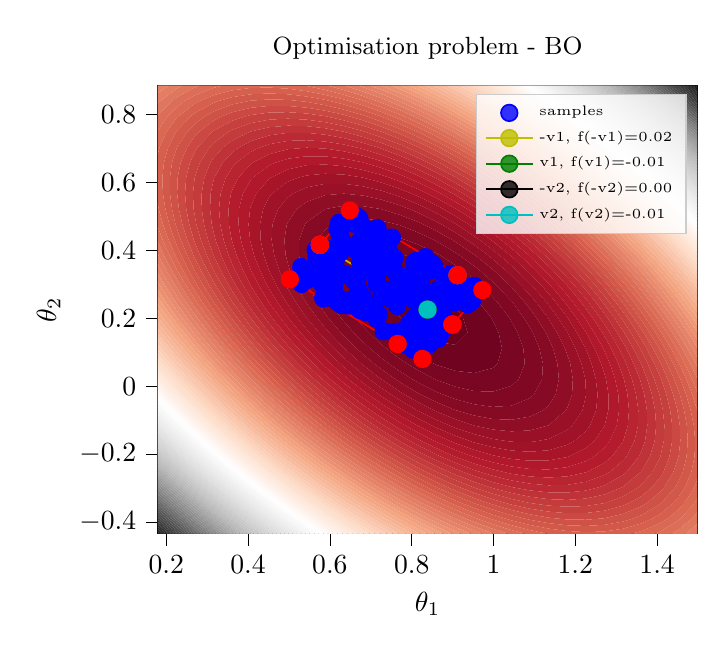
\begin{tikzpicture}

\definecolor{color0}{rgb}{0.415455594002307,0.00369088811995386,0.123414071510957}
\definecolor{color1}{rgb}{0.438523644752018,0.0110726643598616,0.127104959630911}
\definecolor{color2}{rgb}{0.473125720876586,0.0221453287197232,0.132641291810842}
\definecolor{color3}{rgb}{0.507727797001153,0.0332179930795848,0.138177623990773}
\definecolor{color4}{rgb}{0.530795847750865,0.0405997693194925,0.141868512110727}
\definecolor{color5}{rgb}{0.565397923875433,0.0516724336793541,0.147404844290657}
\definecolor{color6}{rgb}{0.6,0.0627450980392157,0.152941176470588}
\definecolor{color7}{rgb}{0.623068050749712,0.0701268742791234,0.156632064590542}
\definecolor{color8}{rgb}{0.657670126874279,0.081199538638985,0.162168396770473}
\definecolor{color9}{rgb}{0.692272202998847,0.0922722029988466,0.167704728950404}
\definecolor{color10}{rgb}{0.706343713956171,0.110726643598616,0.176470588235294}
\definecolor{color11}{rgb}{0.722952710495963,0.143944636678201,0.192156862745098}
\definecolor{color12}{rgb}{0.734025374855825,0.166089965397924,0.202614379084967}
\definecolor{color13}{rgb}{0.750634371395617,0.199307958477509,0.218300653594771}
\definecolor{color14}{rgb}{0.767243367935409,0.232525951557093,0.233986928104575}
\definecolor{color15}{rgb}{0.778316032295271,0.254671280276817,0.244444444444444}
\definecolor{color16}{rgb}{0.794925028835063,0.287889273356401,0.260130718954248}
\definecolor{color17}{rgb}{0.811534025374856,0.321107266435986,0.275816993464052}
\definecolor{color18}{rgb}{0.822606689734717,0.343252595155709,0.286274509803922}
\definecolor{color19}{rgb}{0.83921568627451,0.376470588235294,0.301960784313725}
\definecolor{color20}{rgb}{0.853056516724337,0.408304498269896,0.32641291810842}
\definecolor{color21}{rgb}{0.862283737024221,0.429527104959631,0.342714340638216}
\definecolor{color22}{rgb}{0.876124567474048,0.461361014994233,0.36716647443291}
\definecolor{color23}{rgb}{0.889965397923875,0.493194925028835,0.391618608227605}
\definecolor{color24}{rgb}{0.89919261822376,0.51441753171857,0.407920030757401}
\definecolor{color25}{rgb}{0.913033448673587,0.546251441753172,0.432372164552095}
\definecolor{color26}{rgb}{0.922260668973472,0.567474048442906,0.448673587081891}
\definecolor{color27}{rgb}{0.936101499423299,0.599307958477509,0.473125720876586}
\definecolor{color28}{rgb}{0.949942329873126,0.631141868512111,0.49757785467128}
\definecolor{color29}{rgb}{0.957554786620531,0.65121107266436,0.515109573241061}
\definecolor{color30}{rgb}{0.961707035755479,0.676124567474048,0.546943483275663}
\definecolor{color31}{rgb}{0.965859284890427,0.701038062283737,0.578777393310265}
\definecolor{color32}{rgb}{0.968627450980392,0.717647058823529,0.6}
\definecolor{color33}{rgb}{0.97277970011534,0.742560553633218,0.631833910034602}
\definecolor{color34}{rgb}{0.976931949250288,0.767474048442907,0.663667820069204}
\definecolor{color35}{rgb}{0.979700115340254,0.784083044982699,0.684890426758939}
\definecolor{color36}{rgb}{0.983852364475202,0.808996539792388,0.716724336793541}
\definecolor{color37}{rgb}{0.986620530565167,0.82560553633218,0.737946943483275}
\definecolor{color38}{rgb}{0.990772779700115,0.850519031141868,0.769780853517878}
\definecolor{color39}{rgb}{0.99277201076509,0.869896193771626,0.79761630142253}
\definecolor{color40}{rgb}{0.993387158785083,0.880968858131488,0.814840445982314}
\definecolor{color41}{rgb}{0.994309880815071,0.89757785467128,0.840676662821991}
\definecolor{color42}{rgb}{0.99523260284506,0.914186851211073,0.866512879661669}
\definecolor{color43}{rgb}{0.995847750865052,0.925259515570934,0.883737024221453}
\definecolor{color44}{rgb}{0.99677047289504,0.941868512110727,0.90957324106113}
\definecolor{color45}{rgb}{0.997693194925029,0.958477508650519,0.935409457900807}
\definecolor{color46}{rgb}{0.998308342945021,0.96955017301038,0.952633602460592}
\definecolor{color47}{rgb}{0.99923106497501,0.986159169550173,0.978469819300269}
\definecolor{color48}{rgb}{0.75,0.75,0}
\definecolor{color49}{rgb}{0,0.75,0.75}

\begin{axis}[
legend cell align={left},
legend style={fill opacity=0.8, draw opacity=1, text opacity=1, draw=white!80!black, font=\tiny},
tick align=outside,
tick pos=left,
title={\small{Optimisation problem - BO}},
x grid style={white!69.0196078431373!black},
xlabel={$\theta_1$},
xmin=0.179190742322676, xmax=1.49842955786519,
xtick style={color=black},
y grid style={white!69.0196078431373!black},
ylabel={$\theta_2$},
ymin=-0.434011790585125, ymax=0.885227024957387,
ytick style={color=black}
]
\addplot [draw=none, fill=color0, forget plot]
table{%
x  y
0.816064653274233 0.156178141799354
0.86155564691363 0.131066756212408
0.907046640553027 0.12164768736915
0.93682660766036 0.157371126727036
0.925038562561773 0.202862120366433
0.907046640553027 0.232205689227655
0.894283225595158 0.24835311400583
0.86155564691363 0.27828717635189
0.837628765729934 0.293844107645227
0.816064653274233 0.304823178033463
0.770573659634836 0.308865166769775
0.751668199020553 0.293844107645227
0.750917968387542 0.24835311400583
0.770573659634836 0.204876466875357
0.771773212906136 0.202862120366433
0.814663078853444 0.157371126727036
0.816064653274233 0.156178141799354
};
\addplot [draw=none, fill=color1, forget plot]
table{%
x  y
0.86155564691363 0.0623611968878052
0.907046640553027 0.0454580845785553
0.952537634192424 0.0390122240685854
0.998028627831821 0.0536666824943975
1.00974052767317 0.066389139448242
1.02065993694389 0.111880133087639
1.01267601446049 0.157371126727036
0.998028627831821 0.193705790509703
0.993809852024588 0.202862120366433
0.963605883529315 0.24835311400583
0.952537634192424 0.262129310894546
0.923674221165582 0.293844107645227
0.907046640553027 0.309692516814358
0.871186014155086 0.339335101284624
0.86155564691363 0.346363915443883
0.816064653274233 0.372339140593188
0.785162005851557 0.384826094924021
0.770573659634836 0.389991029930409
0.725082665995439 0.394150378948173
0.694020434586571 0.384826094924021
0.679591672356042 0.374124666818106
0.663745483674934 0.339335101284624
0.665624476057949 0.293844107645227
0.679591672356042 0.248465971229771
0.679631602023247 0.24835311400583
0.707004226255928 0.202862120366433
0.725082665995439 0.178070600077649
0.742265836294037 0.157371126727036
0.770573659634836 0.128340031167654
0.789201093974386 0.111880133087639
0.816064653274233 0.0912146954781101
0.85451049353685 0.066389139448242
0.86155564691363 0.0623611968878052

0.814663078853444 0.157371126727036
0.771773212906136 0.202862120366433
0.770573659634836 0.204876466875357
0.750917968387542 0.24835311400583
0.751668199020553 0.293844107645227
0.770573659634836 0.308865166769775
0.816064653274233 0.304823178033463
0.837628765729934 0.293844107645227
0.86155564691363 0.27828717635189
0.894283225595158 0.24835311400583
0.907046640553027 0.232205689227655
0.925038562561773 0.202862120366433
0.93682660766036 0.157371126727036
0.907046640553027 0.12164768736915
0.86155564691363 0.131066756212408
0.816064653274233 0.156178141799354
0.814663078853444 0.157371126727036
};
\addplot [draw=none, fill=color2, forget plot]
table{%
x  y
0.86155564691363 0.0181447677346222
0.907046640553027 -0.00114068378468596
0.952537634192424 -0.0139391093879813
0.998028627831821 -0.0160465049884528
1.04351962147122 0.00137469580875161
1.06191104140421 0.0208981458088451
1.07637926231879 0.066389139448242
1.07283280861899 0.111880133087639
1.05915837132541 0.157371126727036
1.04351962147122 0.191973720056547
1.03808234422032 0.202862120366433
1.0086534751977 0.24835311400583
0.998028627831821 0.262367347454482
0.971794734347186 0.293844107645227
0.952537634192424 0.314385687730306
0.926569481256145 0.339335101284624
0.907046640553027 0.356218480457703
0.869867367328526 0.384826094924021
0.86155564691363 0.390640745810768
0.816064653274233 0.416707919799359
0.786045502984029 0.430317088563418
0.770573659634837 0.436666020442405
0.725082665995439 0.447239619209083
0.679591672356042 0.447412787675559
0.635322721381952 0.430317088563418
0.634100678716646 0.429339934835332
0.610140362381461 0.384826094924021
0.607754199523372 0.339335101284624
0.617582413573469 0.293844107645227
0.634100678716646 0.250572556011545
0.63503974283437 0.24835311400583
0.662328194995683 0.202862120366433
0.679591672356042 0.178204861493759
0.695672112886268 0.157371126727036
0.725082665995439 0.12391732655182
0.736872565568699 0.111880133087639
0.770573659634836 0.0812146717573715
0.788965441624762 0.066389139448242
0.816064653274233 0.0466875105576706
0.856782041547771 0.0208981458088451
0.86155564691363 0.0181447677346222

0.85451049353685 0.066389139448242
0.816064653274233 0.0912146954781101
0.789201093974386 0.111880133087639
0.770573659634836 0.128340031167654
0.742265836294037 0.157371126727036
0.725082665995439 0.178070600077649
0.707004226255928 0.202862120366433
0.679631602023247 0.24835311400583
0.679591672356042 0.248465971229771
0.665624476057949 0.293844107645227
0.663745483674934 0.339335101284624
0.679591672356042 0.374124666818106
0.694020434586571 0.384826094924021
0.725082665995439 0.394150378948173
0.770573659634836 0.389991029930409
0.785162005851557 0.384826094924021
0.816064653274233 0.372339140593188
0.86155564691363 0.346363915443883
0.871186014155086 0.339335101284624
0.907046640553027 0.309692516814358
0.923674221165581 0.293844107645227
0.952537634192424 0.262129310894546
0.963605883529315 0.24835311400583
0.993809852024588 0.202862120366433
0.998028627831821 0.193705790509703
1.01267601446049 0.157371126727036
1.02065993694389 0.111880133087639
1.00974052767317 0.066389139448242
0.998028627831821 0.0536666824943975
0.952537634192424 0.0390122240685854
0.907046640553027 0.0454580845785553
0.86155564691363 0.0623611968878052
0.85451049353685 0.066389139448242
};
\addplot [draw=none, fill=color3, forget plot]
table{%
x  y
0.907046640553027 -0.0380867394605161
0.952537634192424 -0.0529950533049487
0.998028627831821 -0.0607297292915196
1.04351962147122 -0.0572384216526084
1.08901061511062 -0.0347085436202435
1.09869404035894 -0.0245928478305519
1.11866809110891 0.0208981458088451
1.1207364482184 0.066389139448242
1.11205837089417 0.111880133087639
1.09642530797323 0.157371126727036
1.08901061511062 0.172759894594067
1.07330492196818 0.202862120366433
1.04538440394831 0.24835311400583
1.04351962147122 0.250908491038787
1.00970206481367 0.293844107645227
0.998028627831821 0.307250594261129
0.967684705278356 0.339335101284624
0.952537634192424 0.353955745465892
0.917540531718572 0.384826094924021
0.907046640553027 0.393340787036129
0.86155564691363 0.426299600322912
0.85500056072335 0.430317088563418
0.816064653274233 0.452193453725503
0.770573659634836 0.473905015473031
0.764623247521122 0.475808082202815
0.725082665995439 0.4873585456148
0.679591672356042 0.493330821368111
0.634100678716646 0.488542368030958
0.605939839611156 0.475808082202815
0.588609685077249 0.461376278849742
0.569951224944552 0.430317088563418
0.562052116094754 0.384826094924021
0.566788957317351 0.339335101284624
0.579596770880422 0.293844107645227
0.588609685077249 0.272700947170379
0.599870982093222 0.24835311400583
0.6260184327806 0.202862120366433
0.634100678716646 0.191013940780778
0.65891585851231 0.157371126727036
0.679591672356042 0.132241634946575
0.697826984613922 0.111880133087639
0.725082665995439 0.08430116662934
0.744503255680623 0.066389139448242
0.770573659634836 0.0444058640068708
0.801449369310152 0.0208981458088451
0.816064653274233 0.0106494474415913
0.86155564691363 -0.0169327560665022
0.877140332989053 -0.0245928478305519
0.907046640553027 -0.0380867394605161

0.856782041547771 0.0208981458088451
0.816064653274233 0.0466875105576706
0.788965441624762 0.066389139448242
0.770573659634836 0.0812146717573715
0.7368725655687 0.111880133087639
0.725082665995439 0.12391732655182
0.695672112886268 0.157371126727036
0.679591672356042 0.178204861493759
0.662328194995683 0.202862120366433
0.63503974283437 0.24835311400583
0.634100678716646 0.250572556011545
0.617582413573469 0.293844107645227
0.607754199523372 0.339335101284624
0.610140362381461 0.384826094924021
0.634100678716646 0.429339934835332
0.635322721381951 0.430317088563418
0.679591672356042 0.447412787675559
0.725082665995439 0.447239619209083
0.770573659634836 0.436666020442405
0.786045502984029 0.430317088563418
0.816064653274233 0.416707919799359
0.86155564691363 0.390640745810768
0.869867367328526 0.384826094924021
0.907046640553027 0.356218480457703
0.926569481256146 0.339335101284624
0.952537634192424 0.314385687730306
0.971794734347186 0.293844107645227
0.998028627831821 0.262367347454482
1.0086534751977 0.24835311400583
1.03808234422032 0.202862120366433
1.04351962147122 0.191973720056547
1.05915837132541 0.157371126727036
1.07283280861899 0.111880133087639
1.07637926231879 0.066389139448242
1.06191104140421 0.0208981458088451
1.04351962147122 0.00137469580875161
0.998028627831821 -0.0160465049884528
0.952537634192424 -0.0139391093879813
0.907046640553027 -0.00114068378468596
0.86155564691363 0.0181447677346222
0.856782041547771 0.0208981458088451
};
\addplot [draw=none, fill=color4, forget plot]
table{%
x  y
0.907046640553027 -0.0702533079275928
0.952537634192424 -0.085950903707228
0.998028627831821 -0.0961816852208166
1.04351962147122 -0.0986001463075674
1.08901061511062 -0.0892950962953284
1.12187214948515 -0.0700838414699488
1.13450160875001 -0.056720310550013
1.15178620947877 -0.0245928478305519
1.1597300370884 0.0208981458088451
1.15634373774525 0.066389139448242
1.14534057976068 0.111880133087639
1.13450160875001 0.140929432387971
1.12789743919227 0.157371126727036
1.10419321749571 0.202862120366433
1.08901061511062 0.227830625383644
1.07561437420677 0.24835311400583
1.04351962147122 0.29233368279938
1.042329959325 0.293844107645227
1.00220978729349 0.339335101284624
0.998028627831821 0.343695723673105
0.955590508295244 0.384826094924021
0.952537634192424 0.387572729263868
0.907046640553027 0.424806850659324
0.899548666907747 0.430317088563418
0.86155564691363 0.456166534043793
0.829332664342748 0.475808082202815
0.816064653274233 0.48333702383562
0.770573659634836 0.504443530274076
0.725255984049693 0.521299075842212
0.72508266599544 0.521358939231996
0.679591672356042 0.530133461187015
0.634100678716646 0.531286449054068
0.588609685077249 0.521326836573296
0.588554656472961 0.521299075842212
0.543118691437852 0.482486577475488
0.538780610830543 0.475808082202815
0.525103258035552 0.430317088563418
0.524481171102577 0.384826094924021
0.53254056159923 0.339335101284624
0.543118691437852 0.306195325099809
0.547370050645905 0.293844107645227
0.569110159776139 0.24835311400583
0.588609685077249 0.213606805241822
0.595092921375897 0.202862120366433
0.626950878165432 0.157371126727036
0.634100678716646 0.148270969150689
0.664758384135487 0.111880133087639
0.679591672356042 0.0957246977156465
0.708624526147578 0.066389139448242
0.725082665995439 0.051026113110844
0.760084725181282 0.0208981458088451
0.770573659634837 0.0125088374817104
0.816064653274233 -0.0203630855687107
0.822823232920622 -0.0245928478305519
0.86155564691363 -0.0470585876000581
0.906690132926645 -0.0700838414699488
0.907046640553027 -0.0702533079275928

0.877140332989053 -0.0245928478305519
0.86155564691363 -0.0169327560665022
0.816064653274233 0.0106494474415913
0.801449369310152 0.0208981458088451
0.770573659634836 0.0444058640068708
0.744503255680623 0.066389139448242
0.725082665995439 0.08430116662934
0.697826984613922 0.111880133087639
0.679591672356042 0.132241634946575
0.65891585851231 0.157371126727036
0.634100678716646 0.191013940780778
0.6260184327806 0.202862120366433
0.599870982093222 0.24835311400583
0.588609685077249 0.272700947170379
0.579596770880422 0.293844107645227
0.566788957317351 0.339335101284624
0.562052116094754 0.384826094924021
0.569951224944552 0.430317088563418
0.588609685077249 0.461376278849742
0.605939839611156 0.475808082202815
0.634100678716646 0.488542368030958
0.679591672356042 0.493330821368111
0.725082665995439 0.4873585456148
0.764623247521122 0.475808082202815
0.770573659634837 0.473905015473031
0.816064653274233 0.452193453725503
0.85500056072335 0.430317088563418
0.86155564691363 0.426299600322912
0.907046640553027 0.393340787036129
0.917540531718572 0.384826094924021
0.952537634192424 0.353955745465892
0.967684705278356 0.339335101284624
0.998028627831821 0.307250594261129
1.00970206481367 0.293844107645227
1.04351962147122 0.250908491038787
1.04538440394831 0.24835311400583
1.07330492196818 0.202862120366433
1.08901061511062 0.172759894594067
1.09642530797323 0.157371126727036
1.11205837089417 0.111880133087639
1.1207364482184 0.066389139448242
1.11866809110891 0.0208981458088451
1.09869404035894 -0.0245928478305519
1.08901061511062 -0.0347085436202435
1.04351962147122 -0.0572384216526084
0.998028627831821 -0.0607297292915196
0.952537634192424 -0.0529950533049487
0.907046640553027 -0.0380867394605161
0.877140332989053 -0.0245928478305519
};
\addplot [draw=none, fill=color5, forget plot]
table{%
x  y
0.952537634192424 -0.11568968164537
0.998028627831821 -0.127216244378373
1.04351962147122 -0.132743801367137
1.08901061511061 -0.129927108725732
1.13300976497376 -0.115574835109346
1.13450160875001 -0.114826815311332
1.1778426692813 -0.0700838414699488
1.17999260238941 -0.0652887126137995
1.19204190323151 -0.0245928478305519
1.19392421627799 0.0208981458088451
1.18762036485502 0.066389139448242
1.17999260238941 0.0937436742275861
1.17457583582312 0.111880133087639
1.15532701983799 0.157371126727036
1.13450160875001 0.198857259018273
1.13235359505359 0.202862120366433
1.10319887588767 0.24835311400583
1.08901061511062 0.268328819180591
1.06969099891285 0.293844107645227
1.04351962147122 0.325515038442953
1.03129192624053 0.339335101284624
0.998028627831821 0.374026120626407
0.986885266216191 0.384826094924021
0.952537634192424 0.415728248904686
0.934986902066355 0.430317088563418
0.907046640553027 0.451988152804422
0.873580000447434 0.475808082202815
0.86155564691363 0.483829718017433
0.816064653274233 0.510456513736208
0.79444523380687 0.521299075842212
0.770573659634836 0.53249767665554
0.725082665995439 0.549382785558169
0.679591672356042 0.561435157002923
0.634100678716646 0.566734360855382
0.588609685077249 0.562187088700661
0.543118691437852 0.542470404112493
0.519405780760881 0.521299075842212
0.497627697798455 0.483674769729933
0.494661208407228 0.475808082202815
0.488734375118265 0.430317088563418
0.492005538895898 0.384826094924021
0.497627697798455 0.360017420879019
0.502655276859589 0.339335101284624
0.51978197932303 0.293844107645227
0.540764767699274 0.24835311400583
0.543118691437852 0.244208324467758
0.568082804814826 0.202862120366433
0.588609685077249 0.17222162923509
0.599228934855338 0.157371126727036
0.634100678716646 0.112986900645928
0.635033082514963 0.111880133087639
0.677080106122932 0.066389139448242
0.679591672356042 0.0638636280367025
0.725082665995439 0.0211173194001107
0.725337297412705 0.0208981458088451
0.770573659634836 -0.0152830117682056
0.783287516909047 -0.0245928478305519
0.816064653274233 -0.047007678290798
0.85323893234986 -0.0700838414699488
0.86155564691363 -0.074926394110093
0.907046640553027 -0.0970352383208931
0.952238590598365 -0.115574835109346
0.952537634192424 -0.11568968164537

0.906690132926645 -0.0700838414699488
0.86155564691363 -0.0470585876000582
0.822823232920622 -0.0245928478305519
0.816064653274233 -0.0203630855687107
0.770573659634836 0.0125088374817104
0.760084725181282 0.0208981458088451
0.725082665995439 0.051026113110844
0.708624526147578 0.066389139448242
0.679591672356042 0.0957246977156465
0.664758384135487 0.111880133087639
0.634100678716646 0.148270969150689
0.626950878165432 0.157371126727036
0.595092921375897 0.202862120366433
0.588609685077249 0.213606805241822
0.569110159776139 0.24835311400583
0.547370050645905 0.293844107645227
0.543118691437852 0.306195325099809
0.53254056159923 0.339335101284624
0.524481171102577 0.384826094924021
0.525103258035552 0.430317088563418
0.538780610830543 0.475808082202815
0.543118691437852 0.482486577475488
0.588554656472961 0.521299075842212
0.588609685077249 0.521326836573296
0.634100678716646 0.531286449054068
0.679591672356042 0.530133461187015
0.725082665995439 0.521358939231996
0.725255984049693 0.521299075842212
0.770573659634836 0.504443530274076
0.816064653274233 0.48333702383562
0.829332664342748 0.475808082202815
0.86155564691363 0.456166534043793
0.899548666907747 0.430317088563418
0.907046640553027 0.424806850659324
0.952537634192424 0.387572729263868
0.955590508295244 0.384826094924021
0.998028627831821 0.343695723673105
1.00220978729349 0.339335101284624
1.042329959325 0.293844107645227
1.04351962147122 0.29233368279938
1.07561437420677 0.24835311400583
1.08901061511062 0.227830625383644
1.10419321749571 0.202862120366433
1.12789743919227 0.157371126727036
1.13450160875001 0.140929432387971
1.14534057976068 0.111880133087639
1.15634373774525 0.066389139448242
1.1597300370884 0.0208981458088451
1.15178620947877 -0.0245928478305519
1.13450160875001 -0.056720310550013
1.12187214948515 -0.0700838414699488
1.08901061511062 -0.0892950962953284
1.04351962147122 -0.0986001463075674
0.998028627831821 -0.0961816852208166
0.952537634192424 -0.085950903707228
0.907046640553027 -0.0702533079275928
0.906690132926645 -0.0700838414699488
};
\addplot [draw=none, fill=color6, forget plot]
table{%
x  y
1.04351962147122 -0.16318569142202
1.08901061511062 -0.164129217350652
1.10807655390922 -0.161065828748743
1.13450160875001 -0.155114059034241
1.17999260238941 -0.128779210212724
1.19290003544235 -0.115574835109346
1.21769374824662 -0.0700838414699488
1.22548359602881 -0.0296445603931844
1.22618390836912 -0.0245928478305519
1.22548359602881 -0.00673682231986452
1.22431966319588 0.0208981458088451
1.21491561659772 0.066389139448242
1.2001722995457 0.111880133087639
1.18144665165937 0.157371126727036
1.17999260238941 0.16018628634884
1.15666450468145 0.202862120366433
1.13450160875001 0.239329843228902
1.12867812010469 0.24835311400583
1.09572745948735 0.293844107645227
1.08901061511062 0.302296035425229
1.05781061695038 0.339335101284624
1.04351962147122 0.355123553328348
1.01491967633903 0.384826094924021
0.998028627831821 0.401230190695634
0.966038188069853 0.430317088563418
0.952537634192424 0.441844400589961
0.909852512483537 0.475808082202815
0.907046640553027 0.477912444451764
0.86155564691363 0.508453834356866
0.840402555649491 0.521299075842212
0.816064653274233 0.535206151132027
0.770573659634836 0.557865098509709
0.748669045972825 0.566790069481608
0.725082665995439 0.575817076956661
0.679591672356042 0.588472280953043
0.634100678716646 0.595735107743062
0.588609685077249 0.595640169906171
0.543118691437852 0.58513488124907
0.509575600002874 0.566790069481608
0.497627697798455 0.556404242151293
0.473448560473332 0.521299075842212
0.459473392658038 0.475808082202815
0.457635662956292 0.430317088563418
0.464144500604683 0.384826094924021
0.476638842066038 0.339335101284624
0.493571414353488 0.293844107645227
0.497627697798455 0.285346734368925
0.516335659411035 0.24835311400583
0.542250335794971 0.202862120366433
0.543118691437852 0.201548575457163
0.57400430108435 0.157371126727036
0.588609685077249 0.138138811662657
0.609768830861391 0.111880133087639
0.634100678716646 0.0839051320532168
0.650326485781471 0.066389139448242
0.679591672356042 0.0369614613402375
0.696677585927232 0.0208981458088451
0.725082665995439 -0.00409452784269374
0.750121617575583 -0.0245928478305519
0.770573659634836 -0.0403271614655041
0.812378110632193 -0.0700838414699488
0.816064653274233 -0.0725588116655461
0.86155564691363 -0.0992718942866819
0.892722828991096 -0.115574835109346
0.907046640553027 -0.12262990500612
0.952537634192424 -0.140761513761193
0.998028627831821 -0.154879792108885
1.03131078226358 -0.161065828748743
1.04351962147122 -0.16318569142202

0.952238590598365 -0.115574835109346
0.907046640553027 -0.097035238320893
0.86155564691363 -0.074926394110093
0.85323893234986 -0.0700838414699488
0.816064653274233 -0.047007678290798
0.783287516909047 -0.0245928478305519
0.770573659634836 -0.0152830117682056
0.725337297412706 0.0208981458088451
0.725082665995439 0.0211173194001108
0.679591672356042 0.0638636280367025
0.677080106122932 0.066389139448242
0.635033082514963 0.111880133087639
0.634100678716646 0.112986900645928
0.599228934855338 0.157371126727036
0.588609685077249 0.17222162923509
0.568082804814826 0.202862120366433
0.543118691437852 0.244208324467758
0.540764767699274 0.24835311400583
0.51978197932303 0.293844107645227
0.502655276859589 0.339335101284624
0.497627697798455 0.360017420879019
0.492005538895898 0.384826094924021
0.488734375118265 0.430317088563418
0.494661208407228 0.475808082202815
0.497627697798455 0.483674769729933
0.519405780760881 0.521299075842212
0.543118691437852 0.542470404112493
0.588609685077249 0.562187088700661
0.634100678716646 0.566734360855382
0.679591672356042 0.561435157002923
0.725082665995439 0.549382785558169
0.770573659634836 0.53249767665554
0.79444523380687 0.521299075842212
0.816064653274233 0.510456513736208
0.86155564691363 0.483829718017433
0.873580000447434 0.475808082202815
0.907046640553027 0.451988152804422
0.934986902066355 0.430317088563418
0.952537634192424 0.415728248904686
0.986885266216191 0.384826094924021
0.998028627831821 0.374026120626408
1.03129192624053 0.339335101284624
1.04351962147122 0.325515038442953
1.06969099891285 0.293844107645227
1.08901061511062 0.268328819180591
1.10319887588767 0.24835311400583
1.13235359505359 0.202862120366433
1.13450160875001 0.198857259018273
1.15532701983799 0.157371126727036
1.17457583582312 0.111880133087639
1.17999260238941 0.0937436742275861
1.18762036485502 0.066389139448242
1.19392421627799 0.0208981458088451
1.19204190323151 -0.0245928478305519
1.17999260238941 -0.0652887126137995
1.1778426692813 -0.0700838414699489
1.13450160875001 -0.114826815311332
1.13300976497376 -0.115574835109346
1.08901061511062 -0.129927108725732
1.04351962147122 -0.132743801367137
0.998028627831821 -0.127216244378373
0.952537634192424 -0.11568968164537
0.952238590598365 -0.115574835109346
};
\addplot [draw=none, fill=color7, forget plot]
table{%
x  y
0.952537634192424 -0.165184492714147
0.998028627831821 -0.179362860914326
1.04351962147122 -0.189028527506223
1.08901061511062 -0.192734400930706
1.13450160875001 -0.188340619243071
1.17999260238941 -0.172543623040761
1.1975648797534 -0.161065828748743
1.22548359602881 -0.132367407015267
1.23601157346717 -0.115574835109346
1.25086603023709 -0.0700838414699488
1.25448782678196 -0.0245928478305519
1.25010011810972 0.0208981458088451
1.23980055449905 0.066389139448242
1.22548359602881 0.110310774678794
1.22494123435669 0.111880133087639
1.2041173004923 0.157371126727036
1.1805718217605 0.202862120366433
1.17999260238941 0.20381557562469
1.15148791746285 0.24835311400583
1.13450160875001 0.27275549159441
1.11899172625419 0.293844107645227
1.08901061511062 0.331569886588023
1.08246955694334 0.339335101284624
1.04351962147122 0.382366336526749
1.04115117246244 0.384826094924021
0.998028627831821 0.426705457933033
0.994056473336385 0.430317088563418
0.952537634192424 0.465767531422096
0.939918798078467 0.475808082202815
0.907046640553027 0.500461711823562
0.877071932690807 0.521299075842212
0.86155564691363 0.53149965151506
0.816064653274233 0.558377156903419
0.799731582321365 0.566790069481608
0.770573659634836 0.580971967426142
0.725082665995439 0.59964507896614
0.686177834130742 0.612281063121006
0.679591672356042 0.614297810640286
0.634100678716646 0.622808070794294
0.588609685077249 0.625460413792079
0.543118691437852 0.620283045093799
0.518981175964071 0.612281063121005
0.497627697798455 0.602155534314203
0.458314168183006 0.566790069481608
0.452136704159058 0.557034696302593
0.436772817019514 0.521299075842212
0.429252278352739 0.475808082202815
0.430657032021316 0.430317088563418
0.438608240408372 0.384826094924021
0.451503457431732 0.339335101284624
0.452136704159058 0.337737633161291
0.470511824504062 0.293844107645227
0.492655709196702 0.24835311400583
0.497627697798455 0.239674307496264
0.519864707117269 0.202862120366433
0.543118691437852 0.16768626474211
0.550330274164811 0.157371126727036
0.585180366109251 0.111880133087639
0.588609685077249 0.107770035887983
0.625064030329931 0.066389139448242
0.634100678716646 0.0567698640214294
0.669792325210626 0.0208981458088451
0.679591672356042 0.0116265684661396
0.720278653408467 -0.0245928478305519
0.725082665995439 -0.0286326052353423
0.770573659634836 -0.0639872285889054
0.77913864586305 -0.0700838414699488
0.816064653274233 -0.0948742146350088
0.849609603360511 -0.115574835109346
0.86155564691363 -0.122550314945135
0.907046640553027 -0.145554042750817
0.942558178091423 -0.161065828748743
0.952537634192424 -0.165184492714147

1.03131078226358 -0.161065828748743
0.998028627831821 -0.154879792108885
0.952537634192424 -0.140761513761193
0.907046640553027 -0.12262990500612
0.892722828991096 -0.115574835109346
0.86155564691363 -0.0992718942866819
0.816064653274233 -0.0725588116655461
0.812378110632193 -0.0700838414699488
0.770573659634836 -0.0403271614655041
0.750121617575583 -0.0245928478305519
0.725082665995439 -0.00409452784269374
0.696677585927232 0.0208981458088451
0.679591672356042 0.0369614613402375
0.650326485781471 0.066389139448242
0.634100678716646 0.0839051320532168
0.609768830861391 0.111880133087639
0.588609685077249 0.138138811662657
0.57400430108435 0.157371126727036
0.543118691437852 0.201548575457163
0.542250335794971 0.202862120366433
0.516335659411035 0.24835311400583
0.497627697798455 0.285346734368925
0.493571414353488 0.293844107645227
0.476638842066038 0.339335101284624
0.464144500604683 0.384826094924021
0.457635662956292 0.430317088563418
0.459473392658038 0.475808082202815
0.473448560473332 0.521299075842212
0.497627697798455 0.556404242151293
0.509575600002874 0.566790069481608
0.543118691437852 0.58513488124907
0.588609685077249 0.595640169906171
0.634100678716645 0.595735107743061
0.679591672356042 0.588472280953043
0.725082665995439 0.575817076956661
0.748669045972825 0.566790069481608
0.770573659634836 0.557865098509709
0.816064653274233 0.535206151132027
0.840402555649491 0.521299075842212
0.86155564691363 0.508453834356866
0.907046640553027 0.477912444451764
0.909852512483537 0.475808082202815
0.952537634192424 0.441844400589961
0.966038188069853 0.430317088563418
0.998028627831821 0.401230190695634
1.01491967633903 0.384826094924021
1.04351962147122 0.355123553328348
1.05781061695038 0.339335101284624
1.08901061511062 0.302296035425229
1.09572745948735 0.293844107645227
1.12867812010469 0.24835311400583
1.13450160875001 0.239329843228902
1.15666450468145 0.202862120366433
1.17999260238941 0.16018628634884
1.18144665165937 0.157371126727036
1.2001722995457 0.111880133087639
1.21491561659772 0.066389139448242
1.22431966319588 0.0208981458088451
1.22548359602881 -0.00673682231986453
1.22618390836912 -0.0245928478305519
1.22548359602881 -0.0296445603931844
1.21769374824662 -0.0700838414699488
1.19290003544235 -0.115574835109346
1.17999260238941 -0.128779210212724
1.13450160875001 -0.15511405903424
1.10807655390922 -0.161065828748743
1.08901061511062 -0.164129217350652
1.04351962147122 -0.16318569142202
1.03131078226358 -0.161065828748743
};
\addplot [draw=none, fill=color8, forget plot]
table{%
x  y
1.04351962147122 -0.213709827512023
1.08901061511062 -0.219087330292725
1.13450160875001 -0.218055260312094
1.17999260238941 -0.208485827279882
1.18457478715755 -0.20655682238814
1.22548359602881 -0.1820686189452
1.24616238462361 -0.161065828748743
1.2709745896682 -0.117470531974406
1.27173944899603 -0.115574835109346
1.28063217638885 -0.0700838414699488
1.28103538149715 -0.0245928478305519
1.27505293620336 0.0208981458088451
1.2709745896682 0.0370726601519586
1.26316270095992 0.066389139448242
1.24649952838811 0.111880133087639
1.22662793645489 0.157371126727036
1.22548359602881 0.159540632908528
1.20147193001786 0.202862120366433
1.17999260238941 0.238219325068547
1.17350682721482 0.24835311400583
1.14128293304754 0.293844107645227
1.13450160875001 0.302639475205788
1.10473666921685 0.339335101284624
1.08901061511061 0.357502050138252
1.0640594717846 0.384826094924021
1.04351962147122 0.405986808384932
1.01853157560326 0.430317088563418
0.998028627831821 0.449163837210038
0.967255691226491 0.475808082202815
0.952537634192424 0.487876513726028
0.909098677214667 0.521299075842212
0.907046640553027 0.522798523772802
0.86155564691363 0.552824282705132
0.838493350137894 0.566790069481608
0.816064653274233 0.579672530337321
0.770573659634836 0.602851807021084
0.748806613814096 0.612281063121005
0.725082665995439 0.622015588257016
0.679591672356042 0.636762542312679
0.634100678716646 0.647331413527432
0.588609685077249 0.652457721349674
0.543118691437852 0.650309480707939
0.497627697798455 0.638128592408672
0.45321758023278 0.612281063121005
0.452136704159058 0.611329484800912
0.42002664084582 0.566790069481608
0.406645710519661 0.528707417705115
0.404739150160502 0.521299075842212
0.401293907296288 0.475808082202815
0.404852085707355 0.430317088563418
0.406645710519661 0.421758356111823
0.414832847952346 0.384826094924021
0.429667984424818 0.339335101284624
0.448035538237233 0.293844107645227
0.452136704159058 0.28553131150557
0.471425481264093 0.24835311400583
0.497497109062788 0.202862120366433
0.497627697798455 0.202662558266378
0.528753788698198 0.157371126727036
0.543118691437852 0.137955181615651
0.563430421679556 0.111880133087639
0.588609685077249 0.0817023569909828
0.602099806540553 0.066389139448242
0.634100678716646 0.0323250495127948
0.645470220735936 0.0208981458088451
0.679591672356042 -0.0113856046335693
0.694427992447691 -0.0245928478305519
0.725082665995439 -0.0503707662298027
0.75009720182025 -0.0700838414699488
0.770573659634837 -0.0853741092610934
0.813925130631202 -0.115574835109346
0.816064653274233 -0.116991038174959
0.86155564691363 -0.14366567612567
0.894227005499282 -0.161065828748743
0.907046640553027 -0.167544904563534
0.952537634192424 -0.186844079602618
0.998028627831821 -0.202929875756172
1.01274799010358 -0.20655682238814
1.04351962147122 -0.213709827512023

0.942558178091423 -0.161065828748743
0.907046640553027 -0.145554042750817
0.86155564691363 -0.122550314945135
0.849609603360511 -0.115574835109346
0.816064653274233 -0.0948742146350088
0.77913864586305 -0.0700838414699488
0.770573659634837 -0.0639872285889054
0.725082665995439 -0.0286326052353423
0.720278653408467 -0.0245928478305519
0.679591672356042 0.0116265684661396
0.669792325210626 0.0208981458088451
0.634100678716646 0.0567698640214294
0.625064030329931 0.066389139448242
0.588609685077249 0.107770035887983
0.585180366109251 0.111880133087639
0.550330274164811 0.157371126727036
0.543118691437852 0.16768626474211
0.519864707117269 0.202862120366433
0.497627697798455 0.239674307496264
0.492655709196702 0.24835311400583
0.470511824504062 0.293844107645227
0.452136704159058 0.337737633161291
0.451503457431732 0.339335101284624
0.438608240408372 0.384826094924021
0.430657032021316 0.430317088563418
0.429252278352739 0.475808082202815
0.436772817019514 0.521299075842212
0.452136704159058 0.557034696302593
0.458314168183006 0.566790069481608
0.497627697798455 0.602155534314203
0.518981175964071 0.612281063121005
0.543118691437852 0.620283045093799
0.588609685077249 0.625460413792079
0.634100678716646 0.622808070794294
0.679591672356042 0.614297810640286
0.686177834130742 0.612281063121006
0.725082665995439 0.59964507896614
0.770573659634836 0.580971967426142
0.799731582321365 0.566790069481608
0.816064653274233 0.558377156903419
0.86155564691363 0.53149965151506
0.877071932690807 0.521299075842212
0.907046640553027 0.500461711823562
0.939918798078467 0.475808082202815
0.952537634192424 0.465767531422096
0.994056473336385 0.430317088563418
0.998028627831821 0.426705457933033
1.04115117246244 0.384826094924021
1.04351962147122 0.382366336526749
1.08246955694334 0.339335101284624
1.08901061511062 0.331569886588023
1.11899172625419 0.293844107645227
1.13450160875001 0.27275549159441
1.15148791746285 0.24835311400583
1.17999260238941 0.20381557562469
1.1805718217605 0.202862120366433
1.2041173004923 0.157371126727036
1.22494123435669 0.111880133087639
1.22548359602881 0.110310774678794
1.23980055449905 0.066389139448242
1.25010011810972 0.0208981458088451
1.25448782678196 -0.0245928478305519
1.25086603023709 -0.0700838414699488
1.23601157346717 -0.115574835109346
1.22548359602881 -0.132367407015267
1.1975648797534 -0.161065828748743
1.17999260238941 -0.172543623040761
1.13450160875001 -0.188340619243071
1.08901061511062 -0.192734400930706
1.04351962147122 -0.189028527506223
0.998028627831821 -0.179362860914326
0.952537634192424 -0.165184492714148
0.942558178091423 -0.161065828748743
};
\addplot [draw=none, fill=color9, forget plot]
table{%
x  y
0.952537634192424 -0.208270444631077
0.998028627831821 -0.223924946710233
1.04351962147122 -0.235942435954102
1.08901061511062 -0.243334319859952
1.13450160875001 -0.244718024386169
1.17999260238941 -0.238099010080266
1.22548359602881 -0.220490051787068
1.24601177758432 -0.20655682238814
1.2709745896682 -0.181129851402707
1.2842309875211 -0.161065828748743
1.30112944302723 -0.115574835109346
1.3071138736994 -0.0700838414699488
1.3051325367266 -0.0245928478305519
1.29715950721089 0.0208981458088451
1.28456634538201 0.066389139448242
1.2709745896682 0.104017011416725
1.26798594562161 0.111880133087639
1.24651744033109 0.157371126727036
1.22548359602881 0.197248294564632
1.22237203827522 0.202862120366433
1.19366842447725 0.24835311400583
1.17999260238941 0.268309056004469
1.16162788010926 0.293844107645227
1.13450160875001 0.329026841383407
1.1261402653029 0.339335101284624
1.08901061511062 0.382227771718004
1.08663793803338 0.384826094924021
1.04351962147122 0.429247759530525
1.0424213832789 0.430317088563418
0.998028627831821 0.47112386000765
0.992618556249903 0.475808082202815
0.952537634192424 0.508673416405442
0.936128195706436 0.521299075842212
0.907046640553027 0.542549318836538
0.871539215209541 0.566790069481608
0.86155564691363 0.573279384301435
0.816064653274233 0.599898691734305
0.792488234528101 0.612281063121005
0.770573659634836 0.623226797268453
0.725082665995439 0.642740562744665
0.683321518132065 0.657772056760403
0.679591672356042 0.659047267848543
0.634100678716646 0.669974449672761
0.588609685077249 0.676310239253029
0.543118691437852 0.676754464776539
0.497627697798455 0.669464884179975
0.466511420261498 0.657772056760403
0.452136704159058 0.650274893407121
0.410154520500264 0.612281063121005
0.406645710519661 0.607093029294058
0.387499804562762 0.566790069481608
0.377725219836866 0.521299075842212
0.376756849518802 0.475808082202815
0.38237584550207 0.430317088563418
0.393051029820404 0.384826094924021
0.406645710519661 0.342817537884574
0.407832511417904 0.339335101284624
0.427847296223391 0.293844107645227
0.450420042366756 0.24835311400583
0.452136704159058 0.245376435164441
0.477827323322764 0.202862120366433
0.497627697798455 0.172603734816798
0.508096157900676 0.157371126727036
0.5418505938013 0.111880133087639
0.543118691437852 0.110309410253753
0.580311011190795 0.066389139448242
0.588609685077249 0.0571483011316741
0.622837735241795 0.0208981458088451
0.634100678716646 0.00961354742171597
0.670091995206791 -0.0245928478305519
0.679591672356042 -0.0331591145743753
0.722886601494157 -0.0700838414699488
0.725082665995439 -0.0718655581246758
0.770573659634836 -0.105971923180908
0.784358108394052 -0.115574835109346
0.816064653274233 -0.136562183014052
0.855950477075619 -0.161065828748743
0.86155564691363 -0.164345847392208
0.907046640553027 -0.187582705184814
0.948593864958102 -0.20655682238814
0.952537634192424 -0.208270444631077

1.01274799010358 -0.20655682238814
0.998028627831821 -0.202929875756172
0.952537634192424 -0.186844079602618
0.907046640553027 -0.167544904563534
0.894227005499282 -0.161065828748743
0.86155564691363 -0.14366567612567
0.816064653274233 -0.116991038174959
0.813925130631202 -0.115574835109346
0.770573659634836 -0.0853741092610934
0.75009720182025 -0.0700838414699488
0.725082665995439 -0.0503707662298027
0.694427992447691 -0.0245928478305519
0.679591672356042 -0.0113856046335693
0.645470220735936 0.0208981458088451
0.634100678716646 0.0323250495127948
0.602099806540553 0.066389139448242
0.588609685077249 0.0817023569909828
0.563430421679556 0.111880133087639
0.543118691437852 0.137955181615651
0.528753788698198 0.157371126727036
0.497627697798455 0.202662558266378
0.497497109062788 0.202862120366433
0.471425481264093 0.24835311400583
0.452136704159058 0.28553131150557
0.448035538237233 0.293844107645227
0.429667984424818 0.339335101284624
0.414832847952346 0.384826094924021
0.406645710519661 0.421758356111823
0.404852085707355 0.430317088563418
0.401293907296288 0.475808082202815
0.404739150160502 0.521299075842212
0.406645710519661 0.528707417705115
0.42002664084582 0.566790069481608
0.452136704159058 0.611329484800912
0.45321758023278 0.612281063121005
0.497627697798455 0.638128592408672
0.543118691437852 0.650309480707939
0.588609685077249 0.652457721349674
0.634100678716646 0.647331413527432
0.679591672356042 0.636762542312679
0.725082665995439 0.622015588257016
0.748806613814096 0.612281063121005
0.770573659634836 0.602851807021084
0.816064653274233 0.579672530337321
0.838493350137894 0.566790069481608
0.86155564691363 0.552824282705132
0.907046640553027 0.522798523772802
0.909098677214667 0.521299075842212
0.952537634192424 0.487876513726028
0.967255691226491 0.475808082202815
0.998028627831821 0.449163837210038
1.01853157560326 0.430317088563418
1.04351962147122 0.405986808384932
1.0640594717846 0.384826094924021
1.08901061511062 0.357502050138252
1.10473666921685 0.339335101284624
1.13450160875001 0.302639475205788
1.14128293304754 0.293844107645227
1.17350682721482 0.24835311400583
1.17999260238941 0.238219325068547
1.20147193001786 0.202862120366433
1.22548359602881 0.159540632908528
1.22662793645489 0.157371126727036
1.24649952838811 0.111880133087639
1.26316270095992 0.066389139448242
1.2709745896682 0.0370726601519586
1.27505293620336 0.0208981458088451
1.28103538149715 -0.0245928478305519
1.28063217638885 -0.0700838414699488
1.27173944899603 -0.115574835109346
1.2709745896682 -0.117470531974406
1.24616238462361 -0.161065828748743
1.22548359602881 -0.1820686189452
1.18457478715755 -0.20655682238814
1.17999260238941 -0.208485827279882
1.13450160875001 -0.218055260312094
1.08901061511062 -0.219087330292725
1.04351962147122 -0.213709827512023
1.01274799010358 -0.20655682238814
};
\addplot [draw=none, fill=color10, forget plot]
table{%
x  y
1.04351962147122 -0.257423995560255
1.08901061511062 -0.265527576379288
1.13450160875001 -0.268606591004576
1.17999260238941 -0.265254713470842
1.22548359602881 -0.253486793257071
1.22862271970535 -0.252047816027537
1.2709745896682 -0.225235574110699
1.28947293856998 -0.20655682238814
1.3164655833076 -0.162519861218429
1.31711469834526 -0.161065828748743
1.32836278515444 -0.115574835109346
1.33119046912636 -0.0700838414699488
1.32757806302382 -0.0245928478305519
1.31893004706358 0.0208981458088451
1.3164655833076 0.0292639987005635
1.30498610900899 0.066389139448242
1.28730779523167 0.111880133087639
1.2709745896682 0.147791563720768
1.26640694420728 0.157371126727036
1.24124088534563 0.202862120366433
1.22548359602881 0.228808329258114
1.21305451109332 0.24835311400583
1.18175204346621 0.293844107645227
1.17999260238941 0.296181939391776
1.14602288317533 0.339335101284624
1.13450160875001 0.353127368049795
1.10674648551922 0.384826094924021
1.08901061511062 0.403977964575899
1.06338416267831 0.430317088563418
1.04351962147122 0.449678785902948
1.015282336654 0.475808082202815
0.998028627831821 0.490989105635172
0.96164018472934 0.521299075842212
0.952537634192424 0.528525928103828
0.907046640553027 0.562300113900274
0.900469832559987 0.566790069481608
0.86155564691363 0.592084272328883
0.828132876213174 0.612281063121005
0.816064653274233 0.619240381028835
0.770573659634836 0.642462113227003
0.736755164852512 0.657772056760403
0.725082665995439 0.662809527161151
0.679591672356042 0.678733177577399
0.634100678716646 0.691223462587554
0.588609685077249 0.699391992571824
0.543118691437852 0.702014950489981
0.497627697798455 0.697358283036838
0.452136704159058 0.682880848701088
0.411080104001794 0.657772056760403
0.406645710519661 0.65383018581675
0.375574694576572 0.612281063121005
0.361154716880264 0.576994591778326
0.35803160059769 0.566790069481608
0.3522028389493 0.521299075842212
0.353394269905438 0.475808082202815
0.360052417783098 0.430317088563418
0.361154716880264 0.426041524312944
0.372316260697417 0.384826094924021
0.388447893449477 0.339335101284624
0.406645710519661 0.296137048799311
0.407659054209549 0.293844107645227
0.431647936158264 0.24835311400583
0.452136704159058 0.212825741947124
0.45815753758274 0.202862120366433
0.488590047816183 0.157371126727036
0.497627697798455 0.144900339427264
0.522673302020473 0.111880133087639
0.543118691437852 0.0865555531184631
0.560195901840637 0.066389139448242
0.588609685077249 0.0347494846739829
0.601688368942184 0.0208981458088451
0.634100678716646 -0.0115764821088702
0.647796250400992 -0.0245928478305519
0.679591672356042 -0.053264144909404
0.69931307944384 -0.0700838414699488
0.725082665995439 -0.0909912881854669
0.757225359183295 -0.115574835109346
0.770573659634836 -0.125309772642762
0.816064653274233 -0.156133327853146
0.824093534517134 -0.161065828748743
0.86155564691363 -0.182987809818936
0.905213584303703 -0.20655682238814
0.907046640553027 -0.207501556079191
0.952537634192424 -0.22733532497188
0.998028627831821 -0.244452200647662
1.02410090547965 -0.252047816027537
1.04351962147122 -0.257423995560255

0.948593864958102 -0.20655682238814
0.907046640553027 -0.187582705184814
0.86155564691363 -0.164345847392208
0.855950477075619 -0.161065828748743
0.816064653274233 -0.136562183014052
0.784358108394052 -0.115574835109346
0.770573659634836 -0.105971923180908
0.725082665995439 -0.0718655581246758
0.722886601494157 -0.0700838414699488
0.679591672356042 -0.0331591145743753
0.670091995206791 -0.0245928478305519
0.634100678716646 0.00961354742171597
0.622837735241795 0.0208981458088451
0.588609685077249 0.0571483011316741
0.580311011190795 0.066389139448242
0.543118691437852 0.110309410253753
0.5418505938013 0.111880133087639
0.508096157900676 0.157371126727036
0.497627697798455 0.172603734816798
0.477827323322764 0.202862120366433
0.452136704159058 0.245376435164441
0.450420042366756 0.24835311400583
0.427847296223391 0.293844107645227
0.407832511417904 0.339335101284624
0.406645710519661 0.342817537884574
0.393051029820404 0.384826094924021
0.38237584550207 0.430317088563418
0.376756849518802 0.475808082202815
0.377725219836866 0.521299075842212
0.387499804562762 0.566790069481608
0.406645710519661 0.607093029294058
0.410154520500264 0.612281063121006
0.452136704159058 0.650274893407121
0.466511420261498 0.657772056760403
0.497627697798455 0.669464884179975
0.543118691437852 0.676754464776539
0.588609685077249 0.676310239253029
0.634100678716646 0.669974449672761
0.679591672356042 0.659047267848543
0.683321518132065 0.657772056760403
0.725082665995439 0.642740562744665
0.770573659634836 0.623226797268453
0.792488234528101 0.612281063121005
0.816064653274233 0.599898691734305
0.86155564691363 0.573279384301435
0.871539215209541 0.566790069481608
0.907046640553027 0.542549318836538
0.936128195706436 0.521299075842212
0.952537634192424 0.508673416405442
0.992618556249904 0.475808082202815
0.998028627831821 0.47112386000765
1.0424213832789 0.430317088563418
1.04351962147122 0.429247759530525
1.08663793803338 0.384826094924021
1.08901061511062 0.382227771718004
1.1261402653029 0.339335101284624
1.13450160875001 0.329026841383407
1.16162788010926 0.293844107645227
1.17999260238941 0.268309056004469
1.19366842447725 0.24835311400583
1.22237203827522 0.202862120366433
1.22548359602881 0.197248294564632
1.24651744033109 0.157371126727036
1.26798594562161 0.111880133087639
1.2709745896682 0.104017011416725
1.28456634538201 0.066389139448242
1.29715950721089 0.0208981458088451
1.3051325367266 -0.0245928478305519
1.3071138736994 -0.0700838414699488
1.30112944302723 -0.115574835109346
1.2842309875211 -0.161065828748743
1.2709745896682 -0.181129851402707
1.24601177758432 -0.20655682238814
1.22548359602881 -0.220490051787068
1.17999260238941 -0.238099010080266
1.13450160875001 -0.244718024386169
1.08901061511062 -0.243334319859952
1.04351962147122 -0.235942435954102
0.998028627831821 -0.223924946710233
0.952537634192424 -0.208270444631077
0.948593864958102 -0.20655682238814
};
\addplot [draw=none, fill=color11, forget plot]
table{%
x  y
0.998028627831821 -0.263502045608814
1.04351962147122 -0.276931428166641
1.08901061511062 -0.286568793587077
1.13450160875001 -0.291443364403248
1.17999260238941 -0.290222081907001
1.22548359602881 -0.281023218636588
1.2709745896682 -0.261101720445542
1.28390318346223 -0.252047816027537
1.3164655833076 -0.219115252568472
1.32512399328822 -0.20655682238814
1.34454478575481 -0.161065828748743
1.35324270047632 -0.115574835109346
1.35395405634897 -0.0700838414699488
1.34855713458149 -0.0245928478305519
1.33838405242767 0.0208981458088451
1.32440582608294 0.066389139448242
1.3164655833076 0.0868232203973382
1.3062799204681 0.111880133087639
1.28462221209007 0.157371126727036
1.2709745896682 0.182831691508356
1.25975442597921 0.202862120366433
1.23169758483218 0.24835311400583
1.22548359602881 0.257534346280497
1.19982864562718 0.293844107645227
1.17999260238941 0.32020096165907
1.16493040713018 0.339335101284624
1.13450160875001 0.375761809746726
1.12656500129278 0.384826094924021
1.08901061511062 0.425378754164708
1.08420589982763 0.430317088563418
1.04351962147122 0.469973449070126
1.03721427762725 0.475808082202815
0.998028627831821 0.510286365909084
0.984807388547572 0.521299075842212
0.952537634192424 0.546919229918535
0.926015616412007 0.566790069481608
0.907046640553027 0.580366063008172
0.86155564691363 0.61088916035633
0.859252248942146 0.612281063121005
0.816064653274233 0.637185824115933
0.777444002887014 0.657772056760403
0.770573659634837 0.661274146425384
0.725082665995439 0.681146543693104
0.679591672356042 0.698419087306255
0.663117553084948 0.7032630503998
0.634100678716646 0.711387683415267
0.588609685077249 0.720040437688524
0.543118691437852 0.723986158217942
0.497627697798455 0.7219724939865
0.452136704159058 0.712259592691135
0.430414794755922 0.7032630503998
0.406645710519661 0.689942477692087
0.371272193688709 0.657772056760403
0.361154716880264 0.64354812401473
0.345082683535416 0.612281063121005
0.332682461148666 0.566790069481608
0.329047087662505 0.521299075842212
0.332082559640471 0.475808082202815
0.340312707296719 0.430317088563418
0.352666983635082 0.384826094924021
0.361154716880264 0.36095851676929
0.369204140566507 0.339335101284624
0.3895940598572 0.293844107645227
0.406645710519661 0.260132612810007
0.412875829949773 0.24835311400583
0.439964494374908 0.202862120366433
0.452136704159058 0.184110401530707
0.470267022106436 0.157371126727036
0.497627697798455 0.119616935360637
0.503496010239646 0.111880133087639
0.540416096730449 0.066389139448242
0.543118691437852 0.0632676098087811
0.581470310473121 0.0208981458088451
0.588609685077249 0.0134052467947312
0.626540202733076 -0.0245928478305519
0.634100678716646 -0.0318060819338344
0.676228550564966 -0.0700838414699488
0.679591672356042 -0.0730006881145246
0.725082665995439 -0.110117018246258
0.732218696180544 -0.115574835109346
0.770573659634836 -0.143547173211827
0.79614967944643 -0.161065828748743
0.816064653274233 -0.174101409606132
0.86155564691363 -0.201629772245664
0.870682242523283 -0.20655682238814
0.907046640553027 -0.225298566939711
0.952537634192424 -0.246400205312683
0.967087160917785 -0.252047816027537
0.998028627831821 -0.263502045608814

1.02410090547965 -0.252047816027537
0.998028627831821 -0.244452200647662
0.952537634192424 -0.22733532497188
0.907046640553027 -0.207501556079191
0.905213584303703 -0.20655682238814
0.86155564691363 -0.182987809818936
0.824093534517134 -0.161065828748743
0.816064653274233 -0.156133327853146
0.770573659634836 -0.125309772642762
0.757225359183295 -0.115574835109346
0.725082665995439 -0.0909912881854669
0.69931307944384 -0.0700838414699488
0.679591672356042 -0.053264144909404
0.647796250400992 -0.0245928478305519
0.634100678716646 -0.0115764821088702
0.601688368942184 0.0208981458088451
0.588609685077249 0.0347494846739829
0.560195901840637 0.066389139448242
0.543118691437852 0.0865555531184631
0.522673302020473 0.111880133087639
0.497627697798455 0.144900339427264
0.488590047816183 0.157371126727036
0.45815753758274 0.202862120366433
0.452136704159058 0.212825741947124
0.431647936158264 0.24835311400583
0.407659054209549 0.293844107645227
0.406645710519661 0.296137048799311
0.388447893449477 0.339335101284624
0.372316260697417 0.384826094924021
0.361154716880264 0.426041524312944
0.360052417783098 0.430317088563418
0.353394269905438 0.475808082202815
0.3522028389493 0.521299075842212
0.35803160059769 0.566790069481608
0.361154716880264 0.576994591778326
0.375574694576572 0.612281063121005
0.406645710519661 0.65383018581675
0.411080104001794 0.657772056760403
0.452136704159058 0.682880848701088
0.497627697798455 0.697358283036838
0.543118691437852 0.702014950489981
0.588609685077249 0.699391992571824
0.634100678716646 0.691223462587554
0.679591672356042 0.678733177577399
0.725082665995439 0.662809527161151
0.736755164852512 0.657772056760403
0.770573659634836 0.642462113227003
0.816064653274233 0.619240381028835
0.828132876213174 0.612281063121005
0.86155564691363 0.592084272328883
0.900469832559987 0.566790069481608
0.907046640553027 0.562300113900274
0.952537634192424 0.528525928103828
0.96164018472934 0.521299075842212
0.998028627831821 0.490989105635172
1.015282336654 0.475808082202815
1.04351962147122 0.449678785902948
1.06338416267831 0.430317088563418
1.08901061511062 0.403977964575899
1.10674648551922 0.384826094924021
1.13450160875001 0.353127368049795
1.14602288317533 0.339335101284624
1.17999260238941 0.296181939391776
1.18175204346621 0.293844107645227
1.21305451109332 0.24835311400583
1.22548359602881 0.228808329258114
1.24124088534563 0.202862120366433
1.26640694420728 0.157371126727036
1.2709745896682 0.147791563720768
1.28730779523167 0.111880133087639
1.30498610900899 0.066389139448242
1.3164655833076 0.0292639987005635
1.31893004706358 0.0208981458088451
1.32757806302382 -0.0245928478305519
1.33119046912636 -0.0700838414699488
1.32836278515444 -0.115574835109346
1.31711469834526 -0.161065828748743
1.3164655833076 -0.162519861218429
1.28947293856998 -0.20655682238814
1.2709745896682 -0.225235574110699
1.22862271970535 -0.252047816027537
1.22548359602881 -0.253486793257071
1.17999260238941 -0.265254713470842
1.13450160875001 -0.268606591004576
1.08901061511062 -0.265527576379288
1.04351962147122 -0.257423995560255
1.02410090547965 -0.252047816027537
};
\addplot [draw=none, fill=color12, forget plot]
table{%
x  y
1.08901061511062 -0.306433955056339
1.13450160875001 -0.312179292232312
1.17999260238941 -0.312795871815529
1.22548359602881 -0.306934026518131
1.25648415715172 -0.297538809666934
1.2709745896682 -0.29179653769041
1.3164655833076 -0.260961552940592
1.32533602174153 -0.252047816027537
1.35568673845118 -0.20655682238814
1.361956576947 -0.190195150255545
1.37052518899292 -0.161065828748743
1.37597187977487 -0.115574835109346
1.37490030513622 -0.0700838414699488
1.36866779862278 -0.0245928478305519
1.361956576947 0.00409066311743805
1.35783805779176 0.0208981458088451
1.34254146740934 0.066389139448242
1.32433158406839 0.111880133087639
1.3164655833076 0.128593549971895
1.30233836842721 0.157371126727036
1.27752049465188 0.202862120366433
1.2709745896682 0.213643381982429
1.24901322319255 0.24835311400583
1.22548359602881 0.283118379789621
1.21790524778815 0.293844107645227
1.1834363264391 0.339335101284624
1.17999260238941 0.343579413809256
1.14508929735003 0.384826094924021
1.13450160875001 0.396706560617956
1.10320474304073 0.430317088563418
1.08901061511062 0.444828197280498
1.05728423135817 0.475808082202815
1.04351962147122 0.488632689879044
1.00673107779169 0.521299075842212
0.998028627831821 0.528687716565734
0.952537634192424 0.565312531733242
0.950565534205958 0.566790069481608
0.907046640553027 0.597936306521903
0.885731329693227 0.612281063121005
0.86155564691363 0.627853939270083
0.816064653274233 0.655131267203031
0.811110419442194 0.657772056760403
0.770573659634836 0.678435269988967
0.725082665995439 0.699483560225057
0.715316231424676 0.7032630503998
0.679591672356042 0.716471188751915
0.634100678716646 0.730133743017387
0.588609685077249 0.740198558195785
0.543118691437852 0.745786398029986
0.497627697798455 0.745706120724415
0.452136704159058 0.738302910042932
0.406645710519661 0.721208334192261
0.378463960665394 0.7032630503998
0.361154716880264 0.687758861460697
0.338046735746798 0.657772056760403
0.317081147404787 0.612281063121005
0.315663723240867 0.606209196023979
0.308459677068707 0.566790069481608
0.307112620535558 0.521299075842212
0.311339287822601 0.475808082202815
0.315663723240867 0.453971585142657
0.320572996810341 0.430317088563418
0.334283295421969 0.384826094924021
0.351148103689128 0.339335101284624
0.361154716880264 0.316636550635256
0.371641273641942 0.293844107645227
0.39540519600973 0.24835311400583
0.406645710519661 0.228963794884984
0.422422872652764 0.202862120366433
0.451963563720403 0.157371126727036
0.452136704159058 0.157128169021458
0.48572643741421 0.111880133087639
0.497627697798455 0.0967389914245228
0.522521167040452 0.066389139448242
0.543118691437852 0.0425987491503998
0.562761452842434 0.0208981458088451
0.588609685077249 -0.00623002781533257
0.606939848093755 -0.0245928478305519
0.634100678716646 -0.0505062202357148
0.655647486273985 -0.0700838414699488
0.679591672356042 -0.0908507131948638
0.70960004250873 -0.115574835109346
0.72508266599544 -0.127776398768534
0.76967235561228 -0.161065828748743
0.770573659634836 -0.161710677162059
0.816064653274233 -0.191529338177003
0.840611657898706 -0.20655682238814
0.86155564691363 -0.218833657933859
0.907046640553027 -0.243095577800231
0.926008414835297 -0.252047816027537
0.952537634192424 -0.264029715975869
0.998028627831821 -0.281684109561965
1.04351962147122 -0.296438860773026
1.04831388101174 -0.297538809666934
1.08901061511062 -0.306433955056339

0.967087160917785 -0.252047816027537
0.952537634192424 -0.246400205312683
0.907046640553027 -0.225298566939711
0.870682242523283 -0.20655682238814
0.86155564691363 -0.201629772245664
0.816064653274233 -0.174101409606132
0.79614967944643 -0.161065828748743
0.770573659634836 -0.143547173211827
0.732218696180544 -0.115574835109346
0.725082665995439 -0.110117018246258
0.679591672356042 -0.0730006881145246
0.676228550564966 -0.0700838414699488
0.634100678716646 -0.0318060819338344
0.626540202733076 -0.0245928478305519
0.588609685077249 0.0134052467947312
0.581470310473121 0.0208981458088451
0.543118691437852 0.0632676098087811
0.540416096730449 0.066389139448242
0.503496010239646 0.111880133087639
0.497627697798455 0.119616935360637
0.470267022106436 0.157371126727036
0.452136704159058 0.184110401530707
0.439964494374908 0.202862120366433
0.412875829949773 0.24835311400583
0.406645710519661 0.260132612810007
0.3895940598572 0.293844107645227
0.369204140566507 0.339335101284624
0.361154716880264 0.36095851676929
0.352666983635082 0.384826094924021
0.340312707296719 0.430317088563418
0.332082559640471 0.475808082202815
0.329047087662505 0.521299075842212
0.332682461148666 0.566790069481608
0.345082683535416 0.612281063121005
0.361154716880264 0.64354812401473
0.371272193688709 0.657772056760403
0.406645710519661 0.689942477692087
0.430414794755922 0.7032630503998
0.452136704159058 0.712259592691135
0.497627697798455 0.7219724939865
0.543118691437852 0.723986158217942
0.588609685077249 0.720040437688524
0.634100678716646 0.711387683415267
0.663117553084948 0.703263050399799
0.679591672356042 0.698419087306255
0.725082665995439 0.681146543693104
0.770573659634836 0.661274146425384
0.777444002887014 0.657772056760403
0.816064653274233 0.637185824115933
0.859252248942146 0.612281063121005
0.86155564691363 0.61088916035633
0.907046640553027 0.580366063008172
0.926015616412007 0.566790069481608
0.952537634192424 0.546919229918535
0.984807388547572 0.521299075842212
0.998028627831821 0.510286365909084
1.03721427762725 0.475808082202815
1.04351962147122 0.469973449070126
1.08420589982763 0.430317088563418
1.08901061511062 0.425378754164708
1.12656500129278 0.384826094924021
1.13450160875001 0.375761809746726
1.16493040713018 0.339335101284624
1.17999260238941 0.32020096165907
1.19982864562718 0.293844107645227
1.22548359602881 0.257534346280497
1.23169758483218 0.24835311400583
1.25975442597921 0.202862120366433
1.2709745896682 0.182831691508356
1.28462221209007 0.157371126727036
1.3062799204681 0.111880133087639
1.3164655833076 0.0868232203973382
1.32440582608294 0.066389139448242
1.33838405242767 0.0208981458088451
1.34855713458149 -0.0245928478305519
1.35395405634897 -0.0700838414699488
1.35324270047632 -0.115574835109346
1.34454478575481 -0.161065828748743
1.32512399328822 -0.20655682238814
1.3164655833076 -0.219115252568472
1.28390318346223 -0.252047816027537
1.2709745896682 -0.261101720445542
1.22548359602881 -0.281023218636588
1.17999260238941 -0.290222081907001
1.13450160875001 -0.291443364403248
1.08901061511062 -0.286568793587077
1.04351962147122 -0.27693142816664
0.998028627831821 -0.263502045608814
0.967087160917785 -0.252047816027537
};
\addplot [draw=none, fill=color13, forget plot]
table{%
x  y
0.998028627831821 -0.299627540931506
1.04351962147122 -0.313936354145589
1.08901061511062 -0.325018102454035
1.13450160875001 -0.332150311263594
1.17999260238941 -0.334377450575468
1.22548359602881 -0.33040871813863
1.2709745896682 -0.318456851621449
1.31358465763715 -0.297538809666934
1.3164655833076 -0.295633157773283
1.35983920924571 -0.252047816027537
1.361956576947 -0.248787372495641
1.38239642400775 -0.20655682238814
1.39398604224569 -0.161065828748743
1.39754176159795 -0.115574835109346
1.39486130748888 -0.0700838414699488
1.38724327193498 -0.0245928478305519
1.37564909860436 0.0208981458088451
1.361956576947 0.0626522738165247
1.36067710873573 0.066389139448242
1.34131620709433 0.111880133087639
1.31970098854476 0.157371126727036
1.3164655833076 0.163330540833715
1.29413664911909 0.202862120366433
1.2709745896682 0.241010584654859
1.26632886155292 0.24835311400583
1.234928767506 0.293844107645227
1.22548359602881 0.306644625655248
1.20036915588419 0.339335101284624
1.17999260238941 0.36444874568786
1.1627491098935 0.384826094924021
1.13450160875001 0.416522670158966
1.12165676260412 0.430317088563418
1.08901061511062 0.46369228412347
1.07660287181859 0.475808082202815
1.04351962147122 0.506632036520753
1.02700175453194 0.521299075842212
0.998028627831821 0.545898128386195
0.97214629179732 0.566790069481608
0.952537634192424 0.581953339466959
0.911174734844123 0.612281063121005
0.907046640553027 0.615185851967471
0.86155564691363 0.644671629506965
0.839839898554994 0.657772056760403
0.816064653274233 0.671525824339418
0.770573659634836 0.69559639355255
0.754192584850878 0.7032630503998
0.725082665995439 0.716316537364121
0.679591672356042 0.733990064521712
0.634459941656537 0.748754044039197
0.634100678716646 0.748866550333269
0.588609685077249 0.759052262639639
0.543118691437852 0.765317705198084
0.497627697798455 0.76675521392818
0.452136704159058 0.762153487759312
0.406645710519661 0.749859033045883
0.40417802584944 0.748754044039197
0.361154716880264 0.723246455689078
0.339271083507195 0.7032630503998
0.315663723240867 0.671371984508497
0.308210541151728 0.657772056760403
0.292994767503917 0.612281063121005
0.286538000170956 0.566790069481608
0.286850712139569 0.521299075842212
0.292503503939826 0.475808082202815
0.302442944108074 0.430317088563418
0.315663723240867 0.385589972062515
0.315899607208855 0.384826094924021
0.333946108995067 0.339335101284624
0.354432808281575 0.293844107645227
0.361154716880264 0.280811676687101
0.378581056744788 0.24835311400583
0.405053517563496 0.202862120366433
0.406645710519661 0.200393217562793
0.435501036887704 0.157371126727036
0.452136704159058 0.13402728179734
0.468577568434561 0.111880133087639
0.497627697798455 0.0749216841646293
0.504626237350455 0.066389139448242
0.543118691437852 0.0219298884920184
0.544052595211748 0.0208981458088451
0.58747648851342 -0.0245928478305519
0.588609685077249 -0.0257255507582676
0.634100678716646 -0.0692063585375953
0.635066421983004 -0.0700838414699488
0.679591672356042 -0.108700738275203
0.687934959247196 -0.115574835109346
0.725082665995439 -0.144850242411644
0.746802712333156 -0.161065828748743
0.770573659634836 -0.178073028613486
0.812729245861442 -0.20655682238814
0.816064653274233 -0.208720341913783
0.86155564691363 -0.235520917919123
0.891846565457635 -0.252047816027537
0.907046640553027 -0.260002977800599
0.952537634192424 -0.281055049381155
0.992716612419827 -0.297538809666934
0.998028627831821 -0.299627540931506

1.04831388101174 -0.297538809666934
1.04351962147122 -0.296438860773026
0.998028627831821 -0.281684109561965
0.952537634192424 -0.264029715975869
0.926008414835297 -0.252047816027537
0.907046640553027 -0.243095577800231
0.86155564691363 -0.218833657933859
0.840611657898706 -0.20655682238814
0.816064653274233 -0.191529338177003
0.770573659634836 -0.161710677162059
0.76967235561228 -0.161065828748743
0.725082665995439 -0.127776398768534
0.70960004250873 -0.115574835109346
0.679591672356042 -0.0908507131948638
0.655647486273985 -0.0700838414699488
0.634100678716646 -0.0505062202357148
0.606939848093755 -0.0245928478305519
0.588609685077249 -0.00623002781533257
0.562761452842434 0.0208981458088451
0.543118691437852 0.0425987491503998
0.522521167040452 0.066389139448242
0.497627697798455 0.0967389914245228
0.48572643741421 0.111880133087639
0.452136704159058 0.157128169021458
0.451963563720403 0.157371126727036
0.422422872652764 0.202862120366433
0.406645710519661 0.228963794884984
0.39540519600973 0.24835311400583
0.371641273641942 0.293844107645227
0.361154716880264 0.316636550635256
0.351148103689128 0.339335101284624
0.334283295421969 0.384826094924021
0.320572996810341 0.430317088563418
0.315663723240867 0.453971585142657
0.311339287822601 0.475808082202815
0.307112620535558 0.521299075842212
0.308459677068707 0.566790069481608
0.315663723240867 0.606209196023979
0.317081147404787 0.612281063121005
0.338046735746798 0.657772056760403
0.361154716880264 0.687758861460697
0.378463960665394 0.7032630503998
0.406645710519661 0.721208334192261
0.452136704159058 0.738302910042932
0.497627697798455 0.745706120724415
0.543118691437852 0.745786398029986
0.588609685077249 0.740198558195785
0.634100678716646 0.730133743017387
0.679591672356042 0.716471188751915
0.715316231424676 0.7032630503998
0.725082665995439 0.699483560225057
0.770573659634836 0.678435269988967
0.811110419442194 0.657772056760403
0.816064653274233 0.655131267203031
0.86155564691363 0.627853939270083
0.885731329693227 0.612281063121005
0.907046640553027 0.597936306521902
0.950565534205958 0.566790069481608
0.952537634192424 0.565312531733242
0.998028627831821 0.528687716565734
1.00673107779169 0.521299075842212
1.04351962147122 0.488632689879044
1.05728423135817 0.475808082202815
1.08901061511062 0.444828197280498
1.10320474304073 0.430317088563418
1.13450160875001 0.396706560617956
1.14508929735003 0.384826094924021
1.17999260238941 0.343579413809256
1.1834363264391 0.339335101284624
1.21790524778815 0.293844107645227
1.22548359602881 0.283118379789621
1.24901322319255 0.24835311400583
1.2709745896682 0.213643381982429
1.27752049465188 0.202862120366433
1.30233836842721 0.157371126727036
1.3164655833076 0.128593549971895
1.32433158406839 0.111880133087639
1.34254146740934 0.066389139448242
1.35783805779176 0.0208981458088451
1.361956576947 0.00409066311743805
1.36866779862278 -0.0245928478305519
1.37490030513622 -0.0700838414699488
1.37597187977487 -0.115574835109346
1.37052518899292 -0.161065828748743
1.361956576947 -0.190195150255545
1.35568673845118 -0.20655682238814
1.32533602174153 -0.252047816027537
1.3164655833076 -0.260961552940592
1.2709745896682 -0.29179653769041
1.25648415715172 -0.297538809666934
1.22548359602881 -0.306934026518131
1.17999260238941 -0.312795871815529
1.13450160875001 -0.312179292232312
1.08901061511062 -0.306433955056339
1.04831388101174 -0.297538809666934
};
\addplot [draw=none, fill=color14, forget plot]
table{%
x  y
1.08901061511062 -0.343542392674759
1.13450160875001 -0.351107652441444
1.17999260238941 -0.354415087040257
1.22548359602881 -0.352488250644221
1.2709745896682 -0.344027413861213
1.27391029301055 -0.343029803306331
1.3164655833076 -0.324443336463498
1.35389859918076 -0.297538809666934
1.361956576947 -0.289435644824139
1.38865967281497 -0.252047816027537
1.40744757058639 -0.208268769438576
1.40802074938548 -0.20655682238814
1.41618286621355 -0.161065828748743
1.4177420605225 -0.115574835109346
1.41401388484224 -0.0700838414699488
1.40744757058639 -0.0333186788053437
1.40581874524718 -0.0245928478305519
1.39301890260943 0.0208981458088451
1.37711693635704 0.066389139448242
1.361956576947 0.103326350051534
1.35830083012027 0.111880133087639
1.33567197767518 0.157371126727036
1.3164655833076 0.19274810399652
1.3107528035863 0.202862120366433
1.28242191696952 0.24835311400583
1.2709745896682 0.265439555682531
1.25119210124048 0.293844107645227
1.22548359602881 0.328685421513084
1.21730198532929 0.339335101284624
1.1803680295728 0.384826094924021
1.17999260238941 0.385261041628842
1.13953583762364 0.430317088563418
1.13450160875001 0.435672010495908
1.09518571788382 0.475808082202815
1.08901061511062 0.481841241645582
1.04685537220837 0.521299075842212
1.04351962147122 0.524292794984686
0.998028627831821 0.563108540206655
0.993467702766026 0.566790069481608
0.952537634192424 0.598441072462326
0.933661765131938 0.612281063121005
0.907046640553027 0.631009152058045
0.866813459766105 0.657772056760403
0.86155564691363 0.661134043373198
0.816064653274233 0.687652778983835
0.787118379878914 0.7032630503998
0.770573659634836 0.711833359208283
0.725082665995439 0.73275902906161
0.685922073728754 0.748754044039197
0.679591672356042 0.75123575266893
0.634100678716646 0.765637172974452
0.588609685077249 0.77694412406355
0.543118691437852 0.784491473252001
0.497627697798455 0.787408756051052
0.452136704159058 0.78453431520236
0.406645710519661 0.774282423638039
0.361154716880264 0.754430338736352
0.352534989277773 0.748754044039197
0.315663723240867 0.715524480788087
0.305975045044986 0.7032630503998
0.281993726580759 0.657772056760403
0.27017272960147 0.616343021379869
0.269252642862866 0.612281063121005
0.265278123947572 0.566790069481608
0.266986941169228 0.521299075842212
0.27017272960147 0.499097730194445
0.273667720057051 0.475808082202815
0.28484573143336 0.430317088563418
0.299364105484698 0.384826094924021
0.315663723240867 0.342056227205427
0.316744114301006 0.339335101284624
0.338269765238088 0.293844107645227
0.361154716880264 0.249474781898237
0.361756917479845 0.24835311400583
0.389224508659481 0.202862120366433
0.406645710519661 0.17584827512309
0.419038510055005 0.157371126727036
0.451496423316784 0.111880133087639
0.452136704159058 0.111047286588976
0.48781443417574 0.066389139448242
0.497627697798455 0.0547060142073481
0.527182659111383 0.0208981458088451
0.543118691437852 0.00351821961408703
0.569990107617704 -0.0245928478305519
0.588609685077249 -0.0432043143443587
0.61669487603174 -0.0700838414699488
0.634100678716646 -0.0860324840956021
0.667840197125844 -0.115574835109346
0.679591672356042 -0.125443843119617
0.724075181893718 -0.161065828748743
0.725082665995439 -0.161840930024855
0.770573659634836 -0.194435380064913
0.788513211897089 -0.20655682238814
0.816064653274233 -0.224428126850222
0.861308377383634 -0.252047816027537
0.86155564691363 -0.252192958947619
0.907046640553027 -0.27600995800727
0.951486583860282 -0.297538809666934
0.952537634192424 -0.298028044773106
0.998028627831821 -0.315945335617133
1.04351962147122 -0.331313742539568
1.0870230617705 -0.343029803306331
1.08901061511062 -0.343542392674759

0.992716612419827 -0.297538809666934
0.952537634192424 -0.281055049381155
0.907046640553027 -0.260002977800599
0.891846565457635 -0.252047816027537
0.86155564691363 -0.235520917919123
0.816064653274233 -0.208720341913783
0.812729245861442 -0.20655682238814
0.770573659634836 -0.178073028613486
0.746802712333156 -0.161065828748743
0.725082665995439 -0.144850242411644
0.687934959247196 -0.115574835109346
0.679591672356042 -0.108700738275203
0.635066421983004 -0.0700838414699488
0.634100678716646 -0.0692063585375953
0.588609685077249 -0.0257255507582676
0.58747648851342 -0.0245928478305519
0.544052595211748 0.0208981458088451
0.543118691437852 0.0219298884920184
0.504626237350455 0.066389139448242
0.497627697798455 0.0749216841646293
0.468577568434561 0.111880133087639
0.452136704159058 0.13402728179734
0.435501036887704 0.157371126727036
0.406645710519661 0.200393217562793
0.405053517563496 0.202862120366433
0.378581056744788 0.24835311400583
0.361154716880264 0.280811676687101
0.354432808281575 0.293844107645227
0.333946108995067 0.339335101284624
0.315899607208855 0.384826094924021
0.315663723240867 0.385589972062515
0.302442944108074 0.430317088563418
0.292503503939826 0.475808082202815
0.286850712139569 0.521299075842212
0.286538000170956 0.566790069481608
0.292994767503917 0.612281063121005
0.308210541151728 0.657772056760403
0.315663723240867 0.671371984508497
0.339271083507195 0.7032630503998
0.361154716880264 0.723246455689078
0.40417802584944 0.748754044039197
0.406645710519661 0.749859033045883
0.452136704159058 0.762153487759312
0.497627697798455 0.76675521392818
0.543118691437852 0.765317705198084
0.588609685077249 0.759052262639639
0.634100678716646 0.748866550333269
0.634459941656537 0.748754044039197
0.679591672356042 0.733990064521712
0.725082665995439 0.716316537364121
0.754192584850878 0.7032630503998
0.770573659634836 0.69559639355255
0.816064653274233 0.671525824339418
0.839839898554994 0.657772056760403
0.86155564691363 0.644671629506965
0.907046640553027 0.615185851967471
0.911174734844123 0.612281063121005
0.952537634192424 0.581953339466959
0.97214629179732 0.566790069481608
0.998028627831821 0.545898128386195
1.02700175453194 0.521299075842212
1.04351962147122 0.506632036520753
1.07660287181859 0.475808082202815
1.08901061511062 0.46369228412347
1.12165676260412 0.430317088563418
1.13450160875001 0.416522670158966
1.1627491098935 0.384826094924021
1.17999260238941 0.36444874568786
1.20036915588419 0.339335101284624
1.22548359602881 0.306644625655248
1.234928767506 0.293844107645227
1.26632886155292 0.24835311400583
1.2709745896682 0.241010584654859
1.29413664911909 0.202862120366433
1.3164655833076 0.163330540833715
1.31970098854476 0.157371126727036
1.34131620709433 0.111880133087639
1.36067710873573 0.066389139448242
1.361956576947 0.0626522738165247
1.37564909860436 0.0208981458088451
1.38724327193498 -0.0245928478305519
1.39486130748888 -0.0700838414699488
1.39754176159795 -0.115574835109346
1.39398604224569 -0.161065828748743
1.38239642400775 -0.20655682238814
1.361956576947 -0.248787372495641
1.35983920924571 -0.252047816027537
1.3164655833076 -0.295633157773283
1.31358465763715 -0.297538809666934
1.2709745896682 -0.318456851621449
1.22548359602881 -0.33040871813863
1.17999260238941 -0.334377450575468
1.13450160875001 -0.332150311263594
1.08901061511062 -0.325018102454035
1.04351962147122 -0.313936354145589
0.998028627831821 -0.299627540931506
0.992716612419827 -0.297538809666934
};
\addplot [draw=none, fill=color15, forget plot]
table{%
x  y
1.04351962147122 -0.348133816499527
1.08901061511062 -0.360183311296569
1.13450160875001 -0.36885196305202
1.17999260238941 -0.373419503627561
1.22548359602881 -0.372945426370219
1.2709745896682 -0.36617783987282
1.3164655833076 -0.351412971699462
1.33260459860851 -0.343029803306331
1.361956576947 -0.322916228123013
1.38731369681218 -0.297538809666934
1.40744757058639 -0.267939957119819
1.4156664416346 -0.252047816027537
1.43021568242907 -0.20655682238814
1.43667799869807 -0.161065828748743
1.43677923 -0.115574835109346
1.4317867456546 -0.0700838414699488
1.42265220476552 -0.0245928478305519
1.41010409983244 0.0208981458088451
1.40744757058639 0.0283850256364023
1.39342804319973 0.066389139448242
1.37402153893893 0.111880133087639
1.361956576947 0.136835570745821
1.35164296680559 0.157371126727036
1.32635538759626 0.202862120366433
1.3164655833076 0.21915414684711
1.29806668286826 0.24835311400583
1.2709745896682 0.28879115322474
1.26745543497496 0.293844107645227
1.233407269385 0.339335101284624
1.22548359602881 0.34934052520687
1.19629321434676 0.384826094924021
1.17999260238941 0.403710975324369
1.15610241809946 0.430317088563418
1.13450160875001 0.453293923873957
1.11244752736742 0.475808082202815
1.08901061511062 0.498706264416875
1.06487331835141 0.521299075842212
1.04351962147122 0.540463268898021
1.01284115074281 0.566790069481609
0.998028627831821 0.578998685282452
0.955708943552813 0.612281063121005
0.952537634192424 0.614680247036419
0.907046640553027 0.646832452148619
0.890600926047136 0.657772056760403
0.86155564691363 0.676344387566319
0.816873546391803 0.7032630503998
0.816064653274233 0.703732193366433
0.770573659634836 0.727324079523036
0.72596030884484 0.748754044039196
0.725082665995439 0.749159618081327
0.679591672356042 0.767017379706481
0.634100678716646 0.782407795615634
0.590643242142887 0.794245037678593
0.588609685077249 0.794776262950468
0.543118691437852 0.802652337923001
0.497627697798455 0.806475112762942
0.452136704159058 0.805353019415537
0.406645710519661 0.798112320797975
0.394133706296107 0.794245037678593
0.361154716880264 0.781306559957456
0.315663723240867 0.751639443034657
0.312514818788086 0.748754044039197
0.276910950900462 0.7032630503998
0.27017272960147 0.689758108914677
0.257780725103596 0.657772056760403
0.248440157165739 0.612281063121006
0.245967447703316 0.566790069481608
0.248975923100595 0.521299075842212
0.256428676352107 0.475808082202815
0.267534829685143 0.430317088563418
0.27017272960147 0.422224489543629
0.282852626367173 0.384826094924021
0.301088543187133 0.339335101284624
0.315663723240867 0.307419196087166
0.322106722194601 0.293844107645227
0.346457859716717 0.24835311400583
0.361154716880264 0.223108679271692
0.373395499755466 0.202862120366433
0.402951126970568 0.157371126727036
0.406645710519661 0.152114116117006
0.435987921452247 0.111880133087639
0.452136704159058 0.0908745738907043
0.471698302105035 0.066389139448242
0.497627697798455 0.0355190447525576
0.510409340744651 0.0208981458088451
0.543118691437852 -0.014774855430119
0.552503726721987 -0.0245928478305519
0.588609685077249 -0.0606830779304497
0.598432113793768 -0.0700838414699488
0.634100678716646 -0.102766344266456
0.648728908960971 -0.115574835109346
0.679591672356042 -0.141493696630864
0.704032677268089 -0.161065828748743
0.725082665995439 -0.177260499311617
0.765112817628778 -0.20655682238814
0.770573659634836 -0.210402358847038
0.816064653274233 -0.240135911786661
0.835577505342621 -0.252047816027537
0.86155564691363 -0.267296533999264
0.907046640553027 -0.292016938213942
0.918444910103125 -0.297538809666934
0.952537634192424 -0.31340803778994
0.998028627831821 -0.332263130302761
1.02848269622488 -0.343029803306331
1.04351962147122 -0.348133816499527

1.0870230617705 -0.343029803306331
1.04351962147122 -0.331313742539568
0.998028627831821 -0.315945335617133
0.952537634192424 -0.298028044773106
0.951486583860282 -0.297538809666934
0.907046640553027 -0.27600995800727
0.86155564691363 -0.252192958947619
0.861308377383634 -0.252047816027537
0.816064653274233 -0.224428126850222
0.788513211897089 -0.20655682238814
0.770573659634836 -0.194435380064913
0.725082665995439 -0.161840930024855
0.724075181893718 -0.161065828748743
0.679591672356042 -0.125443843119617
0.667840197125844 -0.115574835109346
0.634100678716646 -0.0860324840956021
0.61669487603174 -0.0700838414699488
0.588609685077249 -0.0432043143443587
0.569990107617704 -0.0245928478305519
0.543118691437852 0.00351821961408703
0.527182659111383 0.0208981458088451
0.497627697798455 0.0547060142073481
0.48781443417574 0.066389139448242
0.452136704159058 0.111047286588976
0.451496423316784 0.111880133087639
0.419038510055005 0.157371126727036
0.406645710519661 0.17584827512309
0.389224508659481 0.202862120366433
0.361756917479845 0.24835311400583
0.361154716880264 0.249474781898237
0.338269765238088 0.293844107645227
0.316744114301006 0.339335101284624
0.315663723240867 0.342056227205427
0.299364105484698 0.384826094924021
0.28484573143336 0.430317088563418
0.273667720057051 0.475808082202815
0.27017272960147 0.499097730194445
0.266986941169228 0.521299075842212
0.265278123947572 0.566790069481608
0.269252642862866 0.612281063121005
0.27017272960147 0.616343021379869
0.281993726580759 0.657772056760403
0.305975045044986 0.7032630503998
0.315663723240867 0.715524480788087
0.352534989277773 0.748754044039197
0.361154716880264 0.754430338736352
0.406645710519661 0.774282423638039
0.452136704159058 0.78453431520236
0.497627697798455 0.787408756051052
0.543118691437852 0.784491473252001
0.588609685077249 0.77694412406355
0.634100678716646 0.765637172974452
0.679591672356042 0.75123575266893
0.685922073728754 0.748754044039197
0.725082665995439 0.73275902906161
0.770573659634836 0.711833359208283
0.787118379878914 0.7032630503998
0.816064653274233 0.687652778983835
0.86155564691363 0.661134043373199
0.866813459766105 0.657772056760403
0.907046640553027 0.631009152058045
0.933661765131938 0.612281063121005
0.952537634192424 0.598441072462326
0.993467702766026 0.566790069481608
0.998028627831821 0.563108540206655
1.04351962147122 0.524292794984685
1.04685537220837 0.521299075842212
1.08901061511062 0.481841241645582
1.09518571788382 0.475808082202815
1.13450160875001 0.435672010495908
1.13953583762364 0.430317088563418
1.17999260238941 0.385261041628842
1.1803680295728 0.384826094924021
1.21730198532929 0.339335101284624
1.22548359602881 0.328685421513084
1.25119210124048 0.293844107645227
1.2709745896682 0.265439555682531
1.28242191696952 0.24835311400583
1.3107528035863 0.202862120366433
1.3164655833076 0.19274810399652
1.33567197767518 0.157371126727036
1.35830083012027 0.111880133087639
1.361956576947 0.103326350051534
1.37711693635704 0.066389139448242
1.39301890260943 0.0208981458088451
1.40581874524718 -0.0245928478305519
1.40744757058639 -0.0333186788053437
1.41401388484224 -0.0700838414699488
1.4177420605225 -0.115574835109346
1.41618286621355 -0.161065828748743
1.40802074938548 -0.20655682238814
1.40744757058639 -0.208268769438576
1.38865967281497 -0.252047816027537
1.361956576947 -0.289435644824139
1.35389859918076 -0.297538809666934
1.3164655833076 -0.324443336463498
1.27391029301055 -0.343029803306331
1.2709745896682 -0.344027413861213
1.22548359602881 -0.352488250644221
1.17999260238941 -0.354415087040257
1.13450160875001 -0.351107652441444
1.08901061511062 -0.343542392674759
1.0870230617705 -0.343029803306331
};
\addplot [draw=none, fill=color16, forget plot]
table{%
x  y
1.17999260238941 -0.392007549938268
1.22548359602881 -0.392846554638596
1.26937587099625 -0.388520796945728
1.2709745896682 -0.388328265884427
1.3164655833076 -0.375562244662881
1.361956576947 -0.352815710182871
1.375276495988 -0.343029803306331
1.40744757058639 -0.310829495346167
1.41722663546019 -0.297538809666934
1.43986862625243 -0.252047816027537
1.45241061547265 -0.20655682238814
1.45293856422579 -0.201860255714381
1.45669790714642 -0.161065828748743
1.45551399514626 -0.115574835109346
1.45293856422579 -0.0954251783793977
1.44955960646695 -0.0700838414699488
1.43931823080597 -0.0245928478305519
1.4257930689575 0.0208981458088451
1.40952967965601 0.066389139448242
1.40744757058639 0.0712505004817165
1.38939559059885 0.111880133087639
1.36710663831882 0.157371126727036
1.361956576947 0.166759625670044
1.34142691540671 0.202862120366433
1.3164655833076 0.243982315638448
1.31371144876699 0.24835311400583
1.28255694026136 0.293844107645227
1.2709745896682 0.309801337415482
1.24873887215024 0.339335101284624
1.22548359602881 0.368700130048982
1.21221839912072 0.384826094924021
1.17999260238941 0.422160909019897
1.17266899857528 0.430317088563418
1.13450160875001 0.470915837252005
1.12970933685103 0.475808082202815
1.08901061511062 0.515571287188169
1.08289126449444 0.521299075842212
1.04351962147122 0.556633742811357
1.031684511866 0.566790069481608
0.998028627831821 0.594529554515999
0.975456976152242 0.612281063121005
0.952537634192424 0.629620184074859
0.913449043468026 0.657772056760403
0.907046640553027 0.662214096850898
0.86155564691363 0.69155473175944
0.842121090536653 0.7032630503998
0.816064653274233 0.718375299486464
0.770573659634836 0.74281479983779
0.75820921615734 0.748754044039196
0.725082665995439 0.76406239966493
0.679591672356042 0.782799006744032
0.647227440347707 0.794245037678593
0.634100678716646 0.798708105588669
0.588609685077249 0.810859931942292
0.543118691437852 0.819764454733122
0.497627697798455 0.824756187438044
0.452136704159058 0.824974468736297
0.406645710519661 0.819286249835329
0.361154716880264 0.806169077276604
0.33618089366204 0.794245037678593
0.315663723240867 0.781516171239284
0.279909635717714 0.748754044039197
0.27017272960147 0.736019582176011
0.251240686168627 0.7032630503998
0.23521313684302 0.657772056760403
0.227627671468612 0.612281063121005
0.22665677145906 0.566790069481608
0.230964905031962 0.521299075842212
0.239553407292068 0.475808082202815
0.251660568786295 0.430317088563418
0.266695292179406 0.384826094924021
0.27017272960147 0.376173011857518
0.285536605821437 0.339335101284624
0.306824841954416 0.293844107645227
0.315663723240867 0.276974312722552
0.331215416949721 0.24835311400583
0.357885653988185 0.202862120366433
0.361154716880264 0.197765555626512
0.388006100837704 0.157371126727036
0.406645710519661 0.130848888276396
0.42047941958771 0.111880133087639
0.452136704159058 0.0707018611924329
0.455582170034331 0.066389139448242
0.494010266515194 0.0208981458088451
0.497627697798455 0.0168233417512075
0.535806043114474 -0.0245928478305519
0.543118691437852 -0.0321941926357884
0.581023839939314 -0.0700838414699488
0.588609685077249 -0.077362444145225
0.630090343403901 -0.115574835109346
0.634100678716645 -0.119126730502395
0.679591672356042 -0.157543550142111
0.68399017264246 -0.161065828748743
0.725082665995439 -0.192680068598379
0.744043699328246 -0.20655682238814
0.770573659634836 -0.225239276394123
0.810698299702157 -0.252047816027537
0.816064653274233 -0.255502698425959
0.86155564691363 -0.28240010905091
0.889067359663864 -0.297538809666934
0.907046640553027 -0.307065699893111
0.952537634192424 -0.328788030806774
0.985806447502889 -0.343029803306331
0.998028627831821 -0.348064681671556
1.04351962147122 -0.36380053382565
1.08901061511062 -0.376824229918379
1.13450160875001 -0.386596273662596
1.15022272451955 -0.388520796945728
1.17999260238941 -0.392007549938268

1.02848269622488 -0.343029803306331
0.998028627831821 -0.332263130302761
0.952537634192424 -0.31340803778994
0.918444910103125 -0.297538809666934
0.907046640553027 -0.292016938213942
0.86155564691363 -0.267296533999264
0.835577505342621 -0.252047816027537
0.816064653274233 -0.240135911786661
0.770573659634836 -0.210402358847038
0.765112817628778 -0.20655682238814
0.725082665995439 -0.177260499311617
0.704032677268089 -0.161065828748743
0.679591672356042 -0.141493696630864
0.648728908960971 -0.115574835109346
0.634100678716646 -0.102766344266456
0.598432113793768 -0.0700838414699488
0.588609685077249 -0.0606830779304497
0.552503726721987 -0.0245928478305519
0.543118691437852 -0.014774855430119
0.510409340744651 0.0208981458088451
0.497627697798455 0.0355190447525576
0.471698302105035 0.066389139448242
0.452136704159058 0.0908745738907043
0.435987921452247 0.111880133087639
0.406645710519661 0.152114116117006
0.402951126970568 0.157371126727036
0.373395499755465 0.202862120366433
0.361154716880264 0.223108679271692
0.346457859716717 0.24835311400583
0.322106722194601 0.293844107645227
0.315663723240867 0.307419196087166
0.301088543187133 0.339335101284624
0.282852626367173 0.384826094924021
0.27017272960147 0.422224489543629
0.267534829685143 0.430317088563418
0.256428676352107 0.475808082202815
0.248975923100595 0.521299075842212
0.245967447703316 0.566790069481609
0.248440157165739 0.612281063121005
0.257780725103596 0.657772056760403
0.27017272960147 0.689758108914677
0.276910950900462 0.7032630503998
0.312514818788086 0.748754044039197
0.315663723240867 0.751639443034657
0.361154716880264 0.781306559957456
0.394133706296107 0.794245037678593
0.406645710519661 0.798112320797975
0.452136704159058 0.805353019415537
0.497627697798455 0.806475112762942
0.543118691437852 0.802652337923001
0.588609685077249 0.794776262950468
0.590643242142887 0.794245037678593
0.634100678716646 0.782407795615634
0.679591672356042 0.767017379706481
0.725082665995439 0.749159618081327
0.72596030884484 0.748754044039197
0.770573659634836 0.727324079523036
0.816064653274233 0.703732193366433
0.816873546391803 0.7032630503998
0.86155564691363 0.676344387566319
0.890600926047136 0.657772056760403
0.907046640553027 0.646832452148619
0.952537634192424 0.614680247036419
0.955708943552813 0.612281063121005
0.998028627831821 0.578998685282452
1.01284115074281 0.566790069481608
1.04351962147122 0.540463268898021
1.06487331835141 0.521299075842212
1.08901061511062 0.498706264416875
1.11244752736742 0.475808082202815
1.13450160875001 0.453293923873957
1.15610241809946 0.430317088563418
1.17999260238941 0.403710975324369
1.19629321434676 0.384826094924021
1.22548359602881 0.34934052520687
1.233407269385 0.339335101284624
1.26745543497496 0.293844107645227
1.2709745896682 0.28879115322474
1.29806668286826 0.24835311400583
1.3164655833076 0.21915414684711
1.32635538759626 0.202862120366433
1.35164296680559 0.157371126727036
1.361956576947 0.136835570745821
1.37402153893893 0.111880133087639
1.39342804319973 0.066389139448242
1.40744757058639 0.0283850256364023
1.41010409983244 0.0208981458088451
1.42265220476552 -0.0245928478305519
1.4317867456546 -0.0700838414699488
1.43677923 -0.115574835109346
1.43667799869807 -0.161065828748743
1.43021568242907 -0.20655682238814
1.4156664416346 -0.252047816027537
1.40744757058639 -0.267939957119819
1.38731369681218 -0.297538809666934
1.361956576947 -0.322916228123013
1.33260459860851 -0.343029803306331
1.3164655833076 -0.351412971699462
1.2709745896682 -0.36617783987282
1.22548359602881 -0.372945426370219
1.17999260238941 -0.373419503627561
1.13450160875001 -0.36885196305202
1.08901061511062 -0.360183311296569
1.04351962147122 -0.348133816499527
1.02848269622488 -0.343029803306331
};
\addplot [draw=none, fill=color17, forget plot]
table{%
x  y
1.08901061511062 -0.392997090361919
1.13450160875001 -0.402753662651038
1.17999260238941 -0.408984647979524
1.22548359602881 -0.410973616768931
1.2709745896682 -0.407795922769352
1.3164655833076 -0.398237133622953
1.34253931088968 -0.388520796945728
1.361956576947 -0.379360363702232
1.40744757058639 -0.346259275532923
1.41068568111782 -0.343029803306331
1.44383523179243 -0.297538809666934
1.45293856422579 -0.278135246428709
1.46262487597921 -0.252047816027537
1.47199658840992 -0.20655682238814
1.47489297455217 -0.161065828748743
1.47255072957418 -0.115574835109346
1.46591047565061 -0.0700838414699488
1.45570036072677 -0.0245928478305519
1.45293856422579 -0.0154870133484464
1.44148203808256 0.0208981458088451
1.42434980880467 0.066389139448242
1.40744757058639 0.105852913681703
1.40476964225877 0.111880133087639
1.38164545114188 0.157371126727036
1.361956576947 0.193263703770684
1.35649844321717 0.202862120366433
1.32822179870319 0.24835311400583
1.3164655833076 0.266049668776575
1.29733762032845 0.293844107645227
1.2709745896682 0.330164967931955
1.26407047491549 0.339335101284624
1.2279056760848 0.384826094924021
1.22548359602881 0.387709034663311
1.18837868391083 0.430317088563418
1.17999260238941 0.439541454645467
1.14577127894241 0.475808082202815
1.13450160875001 0.487268736469391
1.09971914512894 0.521299075842212
1.08901061511062 0.531369163166884
1.04979815912185 0.566790069481608
1.04351962147122 0.572249496723264
0.998028627831821 0.610060423749546
0.995205008751671 0.612281063121005
0.952537634192424 0.644560121113299
0.934192995064671 0.657772056760403
0.907046640553027 0.676606422021771
0.866585384985474 0.7032630503998
0.86155564691363 0.706459569530123
0.816064653274233 0.733018405606495
0.787159148588146 0.748754044039197
0.770573659634836 0.757458280473584
0.725082665995439 0.778965181248533
0.689204922184617 0.794245037678593
0.679591672356042 0.798189485041728
0.634100678716645 0.813879938889395
0.588609685077249 0.826943600934116
0.543118691437852 0.836876571543244
0.521255085321195 0.83973603131799
0.497627697798455 0.84269712229973
0.452136704159058 0.844062498984181
0.406645710519661 0.840375146450782
0.40349675358162 0.83973603131799
0.361154716880264 0.829162263087931
0.315663723240867 0.808682528398455
0.294353472340887 0.794245037678593
0.27017272960147 0.772342074032772
0.251133360551775 0.748754044039197
0.226594720634049 0.7032630503998
0.224681735962073 0.697483691930321
0.214116207912117 0.657772056760403
0.208847773456715 0.612281063121005
0.209191118825673 0.566790069481608
0.214126468933095 0.521299075842212
0.222867021989865 0.475808082202815
0.224681735962073 0.469207346535239
0.235786307887447 0.430317088563418
0.251709933623924 0.384826094924021
0.270001128821506 0.339335101284624
0.27017272960147 0.338969783710397
0.292127046618303 0.293844107645227
0.315663723240867 0.24892225668739
0.315972974182725 0.24835311400583
0.343464593215818 0.202862120366433
0.361154716880264 0.175282699752802
0.37306107470484 0.157371126727036
0.405117133088934 0.111880133087639
0.406645710519661 0.109854347505609
0.440611654679206 0.066389139448242
0.452136704159058 0.0523133396393519
0.478809549976033 0.0208981458088451
0.497627697798455 -0.000299289359823689
0.52002202894327 -0.0245928478305519
0.543118691437852 -0.0486013448493709
0.564609975987605 -0.0700838414699488
0.588609685077249 -0.0931115125612266
0.612994273007766 -0.115574835109346
0.634100678716646 -0.134268470268223
0.665668808410161 -0.161065828748743
0.679591672356042 -0.172445741643898
0.723217024393496 -0.20655682238814
0.725082665995439 -0.207963359369952
0.770573659634836 -0.240076193941207
0.788491719842683 -0.252047816027537
0.816064653274233 -0.26979939372477
0.86155564691363 -0.297503684102555
0.861619480954734 -0.297538809666934
0.907046640553027 -0.321609825935488
0.950361069945594 -0.343029803306331
0.952537634192424 -0.344067718917169
0.998028627831821 -0.362864953785284
1.04351962147122 -0.379467251151773
1.07356350073722 -0.388520796945728
1.08901061511062 -0.392997090361919

1.15022272451955 -0.388520796945728
1.13450160875001 -0.386596273662596
1.08901061511062 -0.376824229918379
1.04351962147122 -0.36380053382565
0.998028627831821 -0.348064681671556
0.985806447502889 -0.343029803306331
0.952537634192424 -0.328788030806774
0.907046640553027 -0.307065699893111
0.889067359663864 -0.297538809666934
0.86155564691363 -0.28240010905091
0.816064653274233 -0.255502698425959
0.810698299702157 -0.252047816027537
0.770573659634836 -0.225239276394123
0.744043699328246 -0.20655682238814
0.725082665995439 -0.192680068598379
0.68399017264246 -0.161065828748743
0.679591672356043 -0.157543550142111
0.634100678716646 -0.119126730502395
0.630090343403901 -0.115574835109346
0.588609685077249 -0.077362444145225
0.581023839939314 -0.0700838414699488
0.543118691437852 -0.0321941926357884
0.535806043114474 -0.0245928478305519
0.497627697798455 0.0168233417512075
0.494010266515194 0.0208981458088451
0.455582170034331 0.066389139448242
0.452136704159058 0.0707018611924329
0.42047941958771 0.111880133087639
0.406645710519661 0.130848888276396
0.388006100837704 0.157371126727036
0.361154716880264 0.197765555626512
0.357885653988185 0.202862120366433
0.331215416949721 0.24835311400583
0.315663723240867 0.276974312722552
0.306824841954416 0.293844107645227
0.285536605821437 0.339335101284624
0.27017272960147 0.376173011857518
0.266695292179406 0.384826094924021
0.251660568786295 0.430317088563418
0.239553407292068 0.475808082202815
0.230964905031962 0.521299075842212
0.22665677145906 0.566790069481608
0.227627671468612 0.612281063121005
0.23521313684302 0.657772056760403
0.251240686168627 0.7032630503998
0.27017272960147 0.736019582176011
0.279909635717714 0.748754044039197
0.315663723240867 0.781516171239284
0.33618089366204 0.794245037678593
0.361154716880264 0.806169077276604
0.406645710519661 0.819286249835329
0.452136704159058 0.824974468736297
0.497627697798455 0.824756187438044
0.543118691437852 0.819764454733122
0.588609685077249 0.810859931942292
0.634100678716646 0.798708105588669
0.647227440347707 0.794245037678593
0.679591672356042 0.782799006744032
0.725082665995439 0.76406239966493
0.75820921615734 0.748754044039197
0.770573659634836 0.74281479983779
0.816064653274233 0.718375299486464
0.842121090536653 0.7032630503998
0.86155564691363 0.69155473175944
0.907046640553027 0.662214096850898
0.913449043468025 0.657772056760402
0.952537634192424 0.629620184074859
0.975456976152242 0.612281063121005
0.998028627831821 0.594529554515999
1.031684511866 0.566790069481608
1.04351962147122 0.556633742811357
1.08289126449444 0.521299075842212
1.08901061511062 0.515571287188169
1.12970933685103 0.475808082202815
1.13450160875001 0.470915837252005
1.17266899857528 0.430317088563418
1.17999260238941 0.422160909019897
1.21221839912072 0.384826094924021
1.22548359602881 0.368700130048982
1.24873887215024 0.339335101284624
1.2709745896682 0.309801337415482
1.28255694026136 0.293844107645227
1.31371144876699 0.24835311400583
1.3164655833076 0.243982315638448
1.34142691540671 0.202862120366433
1.361956576947 0.166759625670044
1.36710663831882 0.157371126727036
1.38939559059885 0.111880133087639
1.40744757058639 0.0712505004817165
1.40952967965601 0.066389139448242
1.4257930689575 0.0208981458088451
1.43931823080597 -0.0245928478305519
1.44955960646695 -0.0700838414699488
1.45293856422579 -0.0954251783793977
1.45551399514626 -0.115574835109346
1.45669790714642 -0.161065828748743
1.45293856422579 -0.201860255714381
1.45241061547265 -0.20655682238814
1.43986862625243 -0.252047816027537
1.41722663546019 -0.297538809666934
1.40744757058639 -0.310829495346167
1.375276495988 -0.343029803306331
1.361956576947 -0.352815710182871
1.3164655833076 -0.375562244662881
1.2709745896682 -0.388328265884427
1.26937587099625 -0.388520796945728
1.22548359602881 -0.392846554638596
1.17999260238941 -0.392007549938268
1.15022272451955 -0.388520796945728
};
\addplot [draw=none, fill=color18, forget plot]
table{%
x  y
1.04351962147122 -0.394541296329662
1.08901061511062 -0.408062692603806
1.13450160875001 -0.418717997994251
1.17999260238941 -0.42596174602078
1.22548359602881 -0.429100678899266
1.2709745896682 -0.427240056616738
1.3164655833076 -0.419204725730774
1.361956576947 -0.403419927949137
1.38931212506247 -0.388520796945728
1.40744757058639 -0.375726833409515
1.4402320598449 -0.343029803306331
1.45293856422579 -0.325047506790125
1.46797591913246 -0.297538809666934
1.48368350976707 -0.252047816027537
1.49151899009903 -0.20655682238814
1.49308804195791 -0.161065828748743
1.4895874640021 -0.115574835109346
1.48192753338445 -0.0700838414699488
1.47081290757146 -0.0245928478305519
1.45679757942734 0.0208981458088451
1.45293856422579 0.0311350307763461
1.43916993795332 0.066389139448242
1.41904405428774 0.111880133087639
1.40744757058639 0.135351955311795
1.39618426396493 0.157371126727036
1.3707523242173 0.202862120366433
1.361956576947 0.217354269677494
1.34248977616754 0.24835311400583
1.3164655833076 0.28752716269528
1.31211830039554 0.293844107645227
1.27867399535711 0.339335101284624
1.2709745896682 0.34925880523139
1.24240652134198 0.384826094924021
1.22548359602881 0.40496901867656
1.20340941475507 0.430317088563418
1.17999260238941 0.45607467858728
1.16137208999769 0.475808082202815
1.13450160875001 0.503133930279878
1.1159349847804 0.521299075842212
1.08901061511062 0.546618214255471
1.06667950990855 0.566790069481608
1.04351962147122 0.586928473180727
1.01311541833925 0.612281063121005
0.998028627831821 0.624407854557944
0.95466478580589 0.657772056760403
0.952537634192424 0.659351762331075
0.907046640553027 0.690998747192643
0.888431041483803 0.7032630503998
0.86155564691363 0.720343007974421
0.816064653274233 0.747661511726526
0.814057731342297 0.748754044039197
0.770573659634836 0.771574935382052
0.725082665995439 0.793867962832136
0.724197278439567 0.794245037678593
0.679591672356042 0.812547325503695
0.634100678716646 0.829051772190121
0.598852230422587 0.83973603131799
0.588609685077249 0.842725179749609
0.543118691437852 0.852604962056633
0.497627697798455 0.859094620298471
0.452136704159058 0.861530306488348
0.406645710519661 0.859062744552474
0.361154716880264 0.850587626932181
0.329435458148893 0.83973603131799
0.315663723240867 0.833836975763232
0.27017272960147 0.803927360755367
0.259637292480738 0.794245037678593
0.224681735962073 0.749737954089456
0.224086952785874 0.748754044039197
0.204948473304409 0.7032630503998
0.19430607375032 0.657772056760403
0.190403019732225 0.612281063121005
0.191935668236582 0.566790069481608
0.197916241021861 0.521299075842212
0.207582623286056 0.475808082202815
0.2203374027928 0.430317088563418
0.224681735962073 0.417937371360245
0.236724575068441 0.384826094924021
0.255810400739025 0.339335101284624
0.27017272960147 0.308759417762732
0.277429251282191 0.293844107645227
0.302013807954608 0.24835311400583
0.315663723240867 0.224988575718014
0.329043532443451 0.202862120366433
0.358372509874722 0.157371126727036
0.361154716880264 0.153365697996024
0.390962578576749 0.111880133087639
0.406645710519661 0.0910956690936086
0.425952660694685 0.066389139448242
0.452136704159058 0.03440998355515
0.463608833436873 0.0208981458088451
0.497627697798455 -0.017421920470855
0.504238014772066 -0.0245928478305519
0.543118691437852 -0.0650084970629535
0.548196112035896 -0.0700838414699488
0.588609685077249 -0.108860580977228
0.595898202611631 -0.115574835109346
0.634100678716646 -0.14941021003405
0.647831363534369 -0.161065828748743
0.679591672356042 -0.187025254145612
0.704570990566817 -0.20655682238814
0.725082665995439 -0.222020901887246
0.766801766591887 -0.252047816027537
0.770573659634836 -0.254668764926945
0.816064653274233 -0.284096089023582
0.838136371878175 -0.297538809666934
0.86155564691363 -0.311301159413223
0.907046640553027 -0.336153951977866
0.920950650427752 -0.343029803306331
0.952537634192424 -0.358092360543674
0.998028627831821 -0.377665225899012
1.02690254757278 -0.388520796945728
1.04351962147122 -0.394541296329662

1.07356350073722 -0.388520796945728
1.04351962147122 -0.379467251151773
0.998028627831821 -0.362864953785284
0.952537634192424 -0.344067718917169
0.950361069945594 -0.343029803306331
0.907046640553027 -0.321609825935488
0.861619480954734 -0.297538809666934
0.86155564691363 -0.297503684102555
0.816064653274233 -0.26979939372477
0.788491719842683 -0.252047816027537
0.770573659634836 -0.240076193941207
0.725082665995439 -0.207963359369952
0.723217024393496 -0.20655682238814
0.679591672356042 -0.172445741643898
0.665668808410161 -0.161065828748743
0.634100678716646 -0.134268470268223
0.612994273007766 -0.115574835109346
0.588609685077249 -0.0931115125612266
0.564609975987605 -0.0700838414699488
0.543118691437852 -0.0486013448493709
0.52002202894327 -0.0245928478305519
0.497627697798455 -0.000299289359823689
0.478809549976033 0.0208981458088451
0.452136704159058 0.0523133396393519
0.440611654679206 0.066389139448242
0.406645710519661 0.109854347505609
0.405117133088934 0.111880133087639
0.37306107470484 0.157371126727036
0.361154716880264 0.175282699752802
0.343464593215818 0.202862120366433
0.315972974182725 0.24835311400583
0.315663723240867 0.24892225668739
0.292127046618303 0.293844107645227
0.27017272960147 0.338969783710397
0.270001128821506 0.339335101284624
0.251709933623924 0.384826094924021
0.235786307887447 0.430317088563418
0.224681735962073 0.469207346535239
0.222867021989865 0.475808082202815
0.214126468933095 0.521299075842212
0.209191118825673 0.566790069481608
0.208847773456715 0.612281063121005
0.214116207912117 0.657772056760403
0.224681735962073 0.697483691930321
0.226594720634049 0.7032630503998
0.251133360551775 0.748754044039197
0.27017272960147 0.772342074032772
0.294353472340887 0.794245037678593
0.315663723240867 0.808682528398455
0.361154716880264 0.829162263087931
0.40349675358162 0.83973603131799
0.406645710519661 0.840375146450782
0.452136704159058 0.844062498984181
0.497627697798455 0.84269712229973
0.521255085321195 0.83973603131799
0.543118691437852 0.836876571543244
0.588609685077249 0.826943600934116
0.634100678716646 0.813879938889395
0.679591672356042 0.798189485041728
0.689204922184617 0.794245037678593
0.725082665995439 0.778965181248533
0.770573659634836 0.757458280473584
0.787159148588146 0.748754044039197
0.816064653274233 0.733018405606495
0.86155564691363 0.706459569530123
0.866585384985474 0.7032630503998
0.907046640553027 0.676606422021771
0.934192995064671 0.657772056760402
0.952537634192424 0.644560121113299
0.995205008751671 0.612281063121005
0.998028627831821 0.610060423749546
1.04351962147122 0.572249496723264
1.04979815912185 0.566790069481608
1.08901061511062 0.531369163166884
1.09971914512894 0.521299075842212
1.13450160875001 0.487268736469391
1.14577127894241 0.475808082202815
1.17999260238941 0.439541454645467
1.18837868391083 0.430317088563418
1.22548359602881 0.387709034663311
1.2279056760848 0.384826094924021
1.26407047491549 0.339335101284624
1.2709745896682 0.330164967931955
1.29733762032845 0.293844107645227
1.3164655833076 0.266049668776575
1.32822179870319 0.24835311400583
1.35649844321717 0.202862120366433
1.361956576947 0.193263703770684
1.38164545114188 0.157371126727036
1.40476964225877 0.111880133087639
1.40744757058639 0.105852913681703
1.42434980880467 0.066389139448242
1.44148203808256 0.0208981458088451
1.45293856422579 -0.0154870133484464
1.45570036072677 -0.0245928478305519
1.46591047565061 -0.0700838414699488
1.47255072957418 -0.115574835109346
1.47489297455217 -0.161065828748743
1.47199658840992 -0.20655682238814
1.46262487597921 -0.252047816027537
1.45293856422579 -0.278135246428709
1.44383523179243 -0.297538809666934
1.41068568111782 -0.343029803306331
1.40744757058639 -0.346259275532923
1.361956576947 -0.379360363702232
1.34253931088968 -0.388520796945728
1.3164655833076 -0.398237133622953
1.2709745896682 -0.407795922769352
1.22548359602881 -0.410973616768931
1.17999260238941 -0.408984647979524
1.13450160875001 -0.402753662651038
1.08901061511062 -0.392997090361919
1.07356350073722 -0.388520796945728
};
\addplot [draw=none, fill=color19, forget plot]
table{%
x  y
0.998028627831821 -0.392129862104382
1.04351962147122 -0.408803963122955
1.08901061511062 -0.423128294845693
1.13200198305404 -0.434011790585125
1.13450160875001 -0.434011790585125
1.17999260238941 -0.434011790585125
1.22548359602881 -0.434011790585125
1.2709745896682 -0.434011790585125
1.3164655833076 -0.434011790585125
1.33739853897795 -0.434011790585125
1.361956576947 -0.42617000036821
1.40744757058639 -0.402589436230385
1.42624065738647 -0.388520796945728
1.45293856422579 -0.361902924945677
1.46718262345821 -0.343029803306331
1.49083320988383 -0.297538809666934
1.49842955786519 -0.273621108497224
1.49842955786519 -0.252047816027537
1.49842955786519 -0.20655682238814
1.49842955786519 -0.161065828748743
1.49842955786519 -0.115574835109346
1.49842955786519 -0.0727778492618888
1.49794459111829 -0.0700838414699488
1.48592545441614 -0.0245928478305519
1.47110231326791 0.0208981458088451
1.45390200059884 0.066389139448242
1.45293856422579 0.0685631186853889
1.43308652495629 0.111880133087639
1.41045352224095 0.157371126727036
1.40744757058639 0.162804244165519
1.38454197524861 0.202862120366433
1.361956576947 0.240074531589481
1.35675775363189 0.24835311400583
1.32602728399374 0.293844107645227
1.3164655833076 0.307201954164917
1.2926810434093 0.339335101284624
1.2709745896682 0.367312380228511
1.25690736659917 0.384826094924021
1.22548359602881 0.422229002689808
1.2184401455993 0.430317088563418
1.17999260238941 0.472607902529092
1.17697290105297 0.475808082202815
1.13450160875001 0.518999124090365
1.13215082443187 0.521299075842212
1.08901061511062 0.561867265344057
1.08356086069525 0.566790069481608
1.04351962147122 0.60160744963819
1.0307192443402 0.612281063121005
0.998028627831821 0.638557844000731
0.973055691817735 0.657772056760403
0.952537634192424 0.673009564855689
0.909893154861777 0.7032630503998
0.907046640553027 0.705214585895273
0.86155564691363 0.734226446418718
0.837414261305245 0.748754044039197
0.816064653274233 0.761162875544635
0.770573659634836 0.78569159029052
0.753135115023229 0.794245037678593
0.725082665995439 0.807526993633209
0.679591672356042 0.826905165965663
0.645413199837525 0.83973603131799
0.634100678716646 0.843833027623725
0.588609685077249 0.857332590414233
0.543118691437852 0.86805574049566
0.497627697798455 0.875492118297212
0.452136704159058 0.878998113992515
0.406645710519661 0.877750342654166
0.361154716880264 0.870678162794571
0.315663723240867 0.856363331447946
0.282663607388465 0.83973603131799
0.27017272960147 0.831691520949108
0.229426819063177 0.794245037678593
0.224681735962073 0.788203371309886
0.200834234692244 0.748754044039197
0.183554652833392 0.7032630503998
0.179190742322676 0.682220229407327
0.179190742322676 0.657772056760403
0.179190742322676 0.612281063121005
0.179190742322676 0.566790069481608
0.179190742322676 0.538244038112925
0.181706013110628 0.521299075842212
0.192298224582246 0.475808082202815
0.205878791645598 0.430317088563418
0.221988176436413 0.384826094924021
0.224681735962073 0.378399543286372
0.241619672656543 0.339335101284624
0.263349967934427 0.293844107645227
0.27017272960147 0.280989260166145
0.288081217054992 0.24835311400583
0.314707523121826 0.202862120366433
0.315663723240867 0.201364590221218
0.344688832623257 0.157371126727036
0.361154716880264 0.133665871958729
0.376808024064565 0.111880133087639
0.406645710519661 0.0723369906816079
0.411293666710165 0.066389139448242
0.448727729273616 0.0208981458088451
0.452136704159058 0.0169507006554308
0.489267862826736 -0.0245928478305519
0.497627697798455 -0.0335778494930381
0.532824426111389 -0.0700838414699488
0.543118691437852 -0.0803565820628298
0.5797376562845 -0.115574835109346
0.588609685077249 -0.123796076850641
0.630400958780069 -0.161065828748743
0.634100678716646 -0.164249083361876
0.679591672356042 -0.201604766647326
0.685924956740137 -0.20655682238814
0.725082665995439 -0.23607844440454
0.747270354616691 -0.252047816027537
0.770573659634836 -0.268240420362923
0.81483983844997 -0.297538809666934
0.816064653274233 -0.298322392149011
0.86155564691363 -0.325095590117969
0.893921186434652 -0.343029803306331
0.907046640553027 -0.35005596731902
0.952537634192424 -0.372117002170179
0.989586265127957 -0.388520796945728
0.998028627831821 -0.392129862104382

1.02690254757278 -0.388520796945728
0.998028627831821 -0.377665225899012
0.952537634192424 -0.358092360543674
0.920950650427752 -0.343029803306331
0.907046640553027 -0.336153951977866
0.86155564691363 -0.311301159413223
0.838136371878175 -0.297538809666934
0.816064653274233 -0.284096089023582
0.770573659634836 -0.254668764926945
0.766801766591887 -0.252047816027537
0.725082665995439 -0.222020901887246
0.704570990566817 -0.20655682238814
0.679591672356042 -0.187025254145612
0.647831363534369 -0.161065828748743
0.634100678716645 -0.14941021003405
0.595898202611631 -0.115574835109346
0.588609685077249 -0.108860580977228
0.548196112035896 -0.0700838414699488
0.543118691437852 -0.0650084970629535
0.504238014772066 -0.0245928478305519
0.497627697798455 -0.017421920470855
0.463608833436873 0.0208981458088451
0.452136704159058 0.03440998355515
0.425952660694685 0.066389139448242
0.406645710519661 0.0910956690936086
0.390962578576749 0.111880133087639
0.361154716880264 0.153365697996024
0.358372509874722 0.157371126727036
0.329043532443451 0.202862120366433
0.315663723240867 0.224988575718014
0.302013807954608 0.24835311400583
0.277429251282191 0.293844107645227
0.27017272960147 0.308759417762732
0.255810400739025 0.339335101284624
0.236724575068441 0.384826094924021
0.224681735962073 0.417937371360245
0.2203374027928 0.430317088563418
0.207582623286056 0.475808082202815
0.197916241021861 0.521299075842212
0.191935668236582 0.566790069481608
0.190403019732225 0.612281063121005
0.19430607375032 0.657772056760403
0.204948473304409 0.7032630503998
0.224086952785874 0.748754044039197
0.224681735962073 0.749737954089456
0.259637292480738 0.794245037678593
0.27017272960147 0.803927360755367
0.315663723240867 0.833836975763232
0.329435458148893 0.83973603131799
0.361154716880264 0.850587626932181
0.406645710519661 0.859062744552474
0.452136704159058 0.861530306488348
0.497627697798455 0.859094620298471
0.543118691437852 0.852604962056633
0.588609685077249 0.842725179749609
0.598852230422587 0.83973603131799
0.634100678716645 0.829051772190121
0.679591672356042 0.812547325503695
0.724197278439567 0.794245037678593
0.725082665995439 0.793867962832136
0.770573659634836 0.771574935382052
0.814057731342297 0.748754044039197
0.816064653274233 0.747661511726526
0.86155564691363 0.720343007974421
0.888431041483803 0.7032630503998
0.907046640553027 0.690998747192643
0.952537634192424 0.659351762331075
0.95466478580589 0.657772056760403
0.998028627831821 0.624407854557944
1.01311541833925 0.612281063121005
1.04351962147122 0.586928473180727
1.06667950990855 0.566790069481608
1.08901061511061 0.546618214255471
1.1159349847804 0.521299075842212
1.13450160875001 0.503133930279878
1.16137208999769 0.475808082202815
1.17999260238941 0.45607467858728
1.20340941475507 0.430317088563418
1.22548359602881 0.40496901867656
1.24240652134198 0.384826094924021
1.2709745896682 0.34925880523139
1.27867399535711 0.339335101284624
1.31211830039554 0.293844107645227
1.3164655833076 0.28752716269528
1.34248977616754 0.24835311400583
1.361956576947 0.217354269677494
1.3707523242173 0.202862120366433
1.39618426396493 0.157371126727036
1.40744757058639 0.135351955311795
1.41904405428774 0.111880133087639
1.43916993795332 0.066389139448242
1.45293856422579 0.0311350307763461
1.45679757942734 0.0208981458088451
1.47081290757146 -0.0245928478305519
1.48192753338445 -0.0700838414699488
1.4895874640021 -0.115574835109346
1.49308804195791 -0.161065828748743
1.49151899009903 -0.20655682238814
1.48368350976707 -0.252047816027537
1.46797591913246 -0.297538809666934
1.45293856422579 -0.325047506790125
1.4402320598449 -0.343029803306331
1.40744757058639 -0.375726833409515
1.38931212506247 -0.388520796945728
1.361956576947 -0.403419927949137
1.3164655833076 -0.419204725730774
1.2709745896682 -0.427240056616738
1.22548359602881 -0.429100678899266
1.17999260238941 -0.42596174602078
1.13450160875001 -0.418717997994251
1.08901061511062 -0.408062692603806
1.04351962147122 -0.394541296329662
1.02690254757278 -0.388520796945728
};
\addplot [draw=none, fill=color20, forget plot]
table{%
x  y
0.998028627831821 -0.405670849245573
1.04351962147122 -0.423066629916247
1.07692633181626 -0.434011790585125
1.08901061511062 -0.434011790585125
1.13200198305404 -0.434011790585125
1.08901061511061 -0.423128294845693
1.04351962147122 -0.408803963122955
0.998028627831821 -0.392129862104382
0.989586265127957 -0.388520796945728
0.952537634192424 -0.372117002170179
0.907046640553027 -0.35005596731902
0.893921186434652 -0.343029803306331
0.86155564691363 -0.325095590117969
0.816064653274233 -0.298322392149011
0.81483983844997 -0.297538809666934
0.770573659634836 -0.268240420362923
0.747270354616691 -0.252047816027537
0.725082665995439 -0.23607844440454
0.685924956740137 -0.20655682238814
0.679591672356042 -0.201604766647326
0.634100678716646 -0.164249083361876
0.63040095878007 -0.161065828748743
0.588609685077249 -0.123796076850641
0.5797376562845 -0.115574835109346
0.543118691437852 -0.0803565820628298
0.532824426111389 -0.0700838414699488
0.497627697798455 -0.0335778494930381
0.489267862826736 -0.0245928478305519
0.452136704159058 0.0169507006554308
0.448727729273616 0.0208981458088451
0.411293666710165 0.066389139448242
0.406645710519661 0.0723369906816079
0.376808024064565 0.111880133087639
0.361154716880264 0.133665871958729
0.344688832623257 0.157371126727036
0.315663723240867 0.201364590221218
0.314707523121826 0.202862120366433
0.288081217054992 0.24835311400583
0.27017272960147 0.280989260166145
0.263349967934427 0.293844107645227
0.241619672656543 0.339335101284624
0.224681735962073 0.378399543286372
0.221988176436413 0.384826094924021
0.205878791645598 0.430317088563418
0.192298224582246 0.475808082202815
0.181706013110628 0.521299075842212
0.179190742322676 0.538244038112925
0.179190742322676 0.521299075842212
0.179190742322676 0.475808082202815
0.179190742322676 0.469251893085382
0.191420180498396 0.430317088563418
0.208270695216462 0.384826094924021
0.224681735962073 0.345671066132383
0.227428944574061 0.339335101284624
0.249873840156676 0.293844107645227
0.27017272960147 0.255598725417086
0.274148626155376 0.24835311400583
0.301464402604739 0.202862120366433
0.315663723240867 0.180624191013843
0.331005155371792 0.157371126727036
0.361154716880264 0.113966045921434
0.36265346955238 0.111880133087639
0.397464766630857 0.066389139448242
0.406645710519661 0.054929114575256
0.434830009496498 0.0208981458088451
0.452136704159058 0.000857743557982965
0.474884157890719 -0.0245928478305519
0.497627697798455 -0.0490371992529348
0.517919515878081 -0.0700838414699488
0.543118691437852 -0.0952303269616861
0.564272347972079 -0.115574835109346
0.588609685077249 -0.138126963416742
0.614331466165107 -0.161065828748743
0.634100678716645 -0.178075342477216
0.668548911611039 -0.20655682238814
0.679591672356042 -0.215376317543576
0.725082665995439 -0.250135986921835
0.727738942641496 -0.252047816027537
0.770573659634836 -0.281812075798901
0.794334775181384 -0.297538809666934
0.816064653274233 -0.311440626883655
0.86155564691363 -0.338890020822715
0.869026635028618 -0.343029803306331
0.907046640553027 -0.363382226328699
0.952537634192424 -0.386141643796685
0.95791104736688 -0.388520796945728
0.998028627831821 -0.405670849245573
};
\addplot [draw=none, fill=color20, forget plot]
table{%
x  y
1.361956576947 -0.434011790585125
1.39439153105031 -0.434011790585125
1.40744757058639 -0.427453207886479
1.45293856422579 -0.393897909638005
1.45834623939348 -0.388520796945728
1.49217451829305 -0.343029803306331
1.49842955786519 -0.33062643031841
1.49842955786519 -0.297538809666934
1.49842955786519 -0.273621108497224
1.49083320988383 -0.297538809666934
1.46718262345821 -0.343029803306331
1.45293856422579 -0.361902924945677
1.42624065738647 -0.388520796945728
1.40744757058639 -0.402589436230385
1.361956576947 -0.42617000036821
1.33739853897795 -0.434011790585125
1.361956576947 -0.434011790585125
};
\addplot [draw=none, fill=color20, forget plot]
table{%
x  y
1.49842955786519 -0.0727778492618888
1.49842955786519 -0.0700838414699488
1.49842955786519 -0.0245928478305519
1.49842955786519 -0.0173425675101523
1.48540704710847 0.0208981458088451
1.46748089971414 0.066389139448242
1.45293856422579 0.0992036939902634
1.44712899562483 0.111880133087639
1.42379587782543 0.157371126727036
1.40744757058639 0.186919929687751
1.39833162627991 0.202862120366433
1.37029217255642 0.24835311400583
1.361956576947 0.260990618534895
1.33957305788111 0.293844107645227
1.3164655833076 0.326125613722684
1.30668809146148 0.339335101284624
1.27137261288502 0.384826094924021
1.2709745896682 0.385310952820313
1.23279321816178 0.430317088563418
1.22548359602881 0.438591586737677
1.19146937264834 0.475808082202815
1.17999260238941 0.487886350441706
1.1471060061687 0.521299075842212
1.13450160875001 0.53363459616403
1.09936417688465 0.566790069481608
1.08901061511062 0.576213393015668
1.04785260285405 0.612281063121005
1.04351962147122 0.615948185898019
0.998028627831821 0.652707833443518
0.99144659782958 0.657772056760403
0.952537634192424 0.686667367380303
0.92914481684346 0.7032630503998
0.907046640553027 0.718413290566679
0.86155564691363 0.748109884863015
0.860485208739912 0.748754044039197
0.816064653274233 0.774572184932037
0.780205907110607 0.794245037678593
0.770573659634836 0.799354980560575
0.725082665995439 0.821153737734306
0.682882813800313 0.83973603131799
0.679591672356042 0.84113664581165
0.634100678716646 0.857684374161967
0.588609685077249 0.871940001078857
0.543118691437852 0.883506518934687
0.533333328258942 0.885227024957387
0.497627697798455 0.885227024957387
0.452136704159058 0.885227024957387
0.406645710519661 0.885227024957387
0.361154716880264 0.885227024957387
0.340402539084829 0.885227024957387
0.315663723240867 0.878084548552429
0.27017272960147 0.856526470563434
0.245985054017934 0.83973603131799
0.224681735962073 0.820357450452313
0.203216128695932 0.794245037678593
0.179190742322676 0.751862936610592
0.179190742322676 0.748754044039197
0.179190742322676 0.7032630503998
0.179190742322676 0.682220229407327
0.183554652833392 0.7032630503998
0.200834234692244 0.748754044039197
0.224681735962073 0.788203371309886
0.229426819063177 0.794245037678593
0.27017272960147 0.831691520949108
0.282663607388465 0.83973603131799
0.315663723240867 0.856363331447946
0.361154716880264 0.870678162794571
0.406645710519661 0.877750342654166
0.452136704159058 0.878998113992515
0.497627697798455 0.875492118297212
0.543118691437852 0.86805574049566
0.588609685077249 0.857332590414233
0.634100678716646 0.843833027623725
0.645413199837525 0.83973603131799
0.679591672356042 0.826905165965663
0.725082665995439 0.807526993633209
0.753135115023229 0.794245037678593
0.770573659634836 0.78569159029052
0.816064653274233 0.761162875544635
0.837414261305246 0.748754044039197
0.86155564691363 0.734226446418718
0.907046640553027 0.705214585895273
0.909893154861777 0.7032630503998
0.952537634192424 0.673009564855689
0.973055691817735 0.657772056760403
0.998028627831821 0.638557844000731
1.0307192443402 0.612281063121005
1.04351962147122 0.60160744963819
1.08356086069525 0.566790069481608
1.08901061511062 0.561867265344057
1.13215082443187 0.521299075842212
1.13450160875001 0.518999124090365
1.17697290105297 0.475808082202815
1.17999260238941 0.472607902529092
1.2184401455993 0.430317088563418
1.22548359602881 0.422229002689808
1.25690736659917 0.384826094924021
1.2709745896682 0.367312380228511
1.2926810434093 0.339335101284624
1.3164655833076 0.307201954164917
1.32602728399374 0.293844107645227
1.35675775363189 0.24835311400583
1.361956576947 0.240074531589481
1.38454197524861 0.202862120366433
1.40744757058639 0.162804244165519
1.41045352224095 0.157371126727036
1.43308652495629 0.111880133087639
1.45293856422579 0.0685631186853889
1.45390200059884 0.066389139448242
1.47110231326791 0.0208981458088451
1.48592545441614 -0.0245928478305519
1.49794459111829 -0.0700838414699489
1.49842955786519 -0.0727778492618888
};
\addplot [draw=none, fill=color21, forget plot]
table{%
x  y
0.952537634192424 -0.399223148035935
0.998028627831821 -0.419211836386764
1.03553724805934 -0.434011790585125
1.04351962147122 -0.434011790585125
1.07692633181626 -0.434011790585125
1.04351962147122 -0.423066629916247
0.998028627831821 -0.405670849245573
0.95791104736688 -0.388520796945728
0.952537634192424 -0.386141643796685
0.907046640553027 -0.363382226328699
0.869026635028618 -0.343029803306331
0.86155564691363 -0.338890020822715
0.816064653274233 -0.311440626883655
0.794334775181384 -0.297538809666934
0.770573659634836 -0.281812075798901
0.727738942641496 -0.252047816027537
0.725082665995439 -0.250135986921835
0.679591672356042 -0.215376317543576
0.668548911611039 -0.20655682238814
0.634100678716646 -0.178075342477216
0.614331466165107 -0.161065828748743
0.588609685077249 -0.138126963416742
0.564272347972079 -0.115574835109346
0.543118691437852 -0.0952303269616861
0.517919515878081 -0.0700838414699488
0.497627697798455 -0.0490371992529348
0.474884157890719 -0.0245928478305519
0.452136704159058 0.000857743557982965
0.434830009496498 0.0208981458088451
0.406645710519661 0.054929114575256
0.397464766630857 0.066389139448242
0.36265346955238 0.111880133087639
0.361154716880264 0.113966045921434
0.331005155371792 0.157371126727036
0.315663723240867 0.180624191013843
0.301464402604739 0.202862120366433
0.274148626155376 0.24835311400583
0.27017272960147 0.255598725417086
0.249873840156676 0.293844107645227
0.227428944574061 0.339335101284624
0.224681735962073 0.345671066132383
0.208270695216462 0.384826094924021
0.191420180498396 0.430317088563418
0.179190742322676 0.469251893085382
0.179190742322676 0.430317088563418
0.179190742322676 0.424812299817498
0.194553213996511 0.384826094924021
0.21415921748916 0.339335101284624
0.224681735962073 0.317444418980896
0.236397712378926 0.293844107645227
0.261003949860335 0.24835311400583
0.27017272960147 0.232704764330877
0.288221282087653 0.202862120366433
0.315663723240867 0.159883791806469
0.317321478120327 0.157371126727036
0.349515095381073 0.111880133087639
0.361154716880264 0.0962063872126765
0.384021265167039 0.066389139448242
0.406645710519661 0.0381483932222743
0.42093228971938 0.0208981458088451
0.452136704159058 -0.015235213539465
0.460500452954703 -0.0245928478305519
0.497627697798455 -0.0644965490128315
0.503014605644773 -0.0700838414699488
0.543118691437852 -0.110104071860542
0.548807039659658 -0.115574835109346
0.588609685077249 -0.152457849982844
0.598261973550145 -0.161065828748743
0.634100678716646 -0.191901601592557
0.651826108036468 -0.20655682238814
0.679591672356042 -0.228732278839574
0.710021865436522 -0.252047816027537
0.725082665995439 -0.263207759864802
0.770573659634836 -0.29538373123488
0.773829711912799 -0.297538809666934
0.816064653274233 -0.324558861618298
0.846451303300228 -0.343029803306331
0.86155564691363 -0.351914358050988
0.907046640553027 -0.376708485338378
0.930534547494435 -0.388520796945728
0.952537634192424 -0.399223148035935
};
\addplot [draw=none, fill=color21, forget plot]
table{%
x  y
1.40744757058639 -0.434011790585125
1.43536469131107 -0.434011790585125
1.45293856422579 -0.42130837565339
1.48591250123118 -0.388520796945728
1.49842955786519 -0.371361502045477
1.49842955786519 -0.343029803306331
1.49842955786519 -0.33062643031841
1.49217451829305 -0.343029803306331
1.45834623939348 -0.388520796945728
1.45293856422579 -0.393897909638005
1.40744757058639 -0.427453207886479
1.39439153105031 -0.434011790585125
1.40744757058639 -0.434011790585125
};
\addplot [draw=none, fill=color21, forget plot]
table{%
x  y
1.49842955786519 -0.0173425675101523
1.49842955786519 0.0208981458088451
1.49842955786519 0.023877117261564
1.48105979882944 0.066389139448242
1.46051523398384 0.111880133087639
1.45293856422579 0.126944005289363
1.4371382334099 0.157371126727036
1.41175492447683 0.202862120366433
1.40744757058639 0.209960053118219
1.38340608465338 0.24835311400583
1.361956576947 0.280872475967128
1.35311883176848 0.293844107645227
1.32035879071207 0.339335101284624
1.3164655833076 0.344442022253066
1.28468298590905 0.384826094924021
1.2709745896682 0.401525181515283
1.24654870903588 0.430317088563418
1.22548359602881 0.454162813547114
1.20570078214524 0.475808082202815
1.17999260238941 0.502863628669214
1.1618474466124 0.521299075842212
1.13450160875001 0.548061572093604
1.11465356451887 0.566790069481608
1.08901061511062 0.590129072417539
1.06373224525146 0.612281063121006
1.04351962147122 0.629387569357427
1.00863445465985 0.657772056760402
0.998028627831821 0.666115951019072
0.952537634192424 0.700325169904916
0.948396478825143 0.7032630503998
0.907046640553027 0.731611995238085
0.880815502375533 0.748754044039196
0.86155564691363 0.760931038112808
0.816064653274233 0.78798149431944
0.8046477624809 0.794245037678593
0.770573659634836 0.812321475159683
0.725082665995439 0.834780481835403
0.713828756203893 0.83973603131799
0.679591672356042 0.854306342764616
0.634100678716646 0.871535720700208
0.592421198051386 0.885227024957387
0.588609685077249 0.885227024957387
0.543118691437852 0.885227024957387
0.533333328258942 0.885227024957387
0.543118691437852 0.883506518934687
0.588609685077249 0.871940001078857
0.634100678716646 0.857684374161967
0.679591672356042 0.84113664581165
0.682882813800313 0.83973603131799
0.725082665995439 0.821153737734306
0.770573659634836 0.799354980560575
0.780205907110607 0.794245037678593
0.816064653274233 0.774572184932037
0.860485208739912 0.748754044039197
0.86155564691363 0.748109884863015
0.907046640553027 0.718413290566679
0.92914481684346 0.7032630503998
0.952537634192424 0.686667367380303
0.99144659782958 0.657772056760402
0.998028627831821 0.652707833443518
1.04351962147122 0.615948185898019
1.04785260285405 0.612281063121005
1.08901061511062 0.576213393015668
1.09936417688465 0.566790069481608
1.13450160875001 0.53363459616403
1.1471060061687 0.521299075842212
1.17999260238941 0.487886350441706
1.19146937264834 0.475808082202815
1.22548359602881 0.438591586737677
1.23279321816178 0.430317088563418
1.2709745896682 0.385310952820313
1.27137261288502 0.384826094924021
1.30668809146148 0.339335101284624
1.3164655833076 0.326125613722684
1.33957305788111 0.293844107645227
1.361956576947 0.260990618534895
1.37029217255642 0.24835311400583
1.39833162627991 0.202862120366433
1.40744757058639 0.186919929687751
1.42379587782543 0.157371126727036
1.44712899562483 0.111880133087639
1.45293856422579 0.0992036939902634
1.46748089971414 0.066389139448242
1.48540704710847 0.0208981458088451
1.49842955786519 -0.0173425675101523
};
\addplot [draw=none, fill=color21, forget plot]
table{%
x  y
0.203216128695932 0.794245037678593
0.224681735962073 0.820357450452313
0.245985054017934 0.83973603131799
0.27017272960147 0.856526470563434
0.315663723240867 0.878084548552429
0.340402539084829 0.885227024957387
0.315663723240867 0.885227024957387
0.281173271105543 0.885227024957387
0.27017272960147 0.880166466662458
0.224681735962073 0.849445537208291
0.214143650943851 0.83973603131799
0.179190742322676 0.796226092772996
0.179190742322676 0.794245037678593
0.179190742322676 0.751862936610592
0.203216128695932 0.794245037678593
};
\addplot [draw=none, fill=color22, forget plot]
table{%
x  y
0.907046640553027 -0.389917767603951
0.952537634192424 -0.412111970938614
0.998028627831821 -0.432752823527955
1.00121932130245 -0.434011790585125
1.03553724805934 -0.434011790585125
0.998028627831821 -0.419211836386764
0.952537634192424 -0.399223148035935
0.930534547494435 -0.388520796945728
0.907046640553027 -0.376708485338378
0.86155564691363 -0.351914358050988
0.846451303300228 -0.343029803306331
0.816064653274233 -0.324558861618298
0.773829711912799 -0.297538809666934
0.770573659634837 -0.29538373123488
0.725082665995439 -0.263207759864802
0.710021865436522 -0.252047816027537
0.679591672356042 -0.228732278839574
0.651826108036468 -0.20655682238814
0.634100678716646 -0.191901601592557
0.598261973550145 -0.161065828748743
0.588609685077249 -0.152457849982844
0.548807039659658 -0.115574835109346
0.543118691437852 -0.110104071860542
0.503014605644773 -0.0700838414699488
0.497627697798455 -0.0644965490128315
0.460500452954703 -0.0245928478305519
0.452136704159058 -0.015235213539465
0.42093228971938 0.0208981458088451
0.406645710519661 0.0381483932222743
0.384021265167039 0.066389139448242
0.361154716880264 0.0962063872126765
0.349515095381073 0.111880133087639
0.317321478120327 0.157371126727036
0.315663723240867 0.159883791806469
0.288221282087653 0.202862120366433
0.27017272960147 0.232704764330877
0.261003949860335 0.24835311400583
0.236397712378926 0.293844107645227
0.224681735962073 0.317444418980896
0.21415921748916 0.339335101284624
0.194553213996511 0.384826094924021
0.179190742322676 0.424812299817498
0.179190742322676 0.389107757844765
0.18083573277656 0.384826094924021
0.201110592127268 0.339335101284624
0.223056659498467 0.293844107645227
0.224681735962073 0.290815165084478
0.248173902783821 0.24835311400583
0.27017272960147 0.21080773237376
0.274978161570566 0.202862120366433
0.30457378338922 0.157371126727036
0.315663723240867 0.141244998225066
0.336497061510641 0.111880133087639
0.361154716880264 0.0786764911854738
0.370577763703222 0.066389139448242
0.406645710519661 0.0213676718692927
0.407034569942262 0.0208981458088451
0.44660729978377 -0.0245928478305519
0.452136704159058 -0.0307096369511585
0.488911032866209 -0.0700838414699488
0.497627697798455 -0.0790818390834737
0.53419312443931 -0.115574835109346
0.543118691437852 -0.124174129403958
0.582771163962724 -0.161065828748743
0.588609685077249 -0.166315968700561
0.634100678716646 -0.205727860707897
0.635103304461896 -0.20655682238814
0.679591672356042 -0.242088240135573
0.692590378538485 -0.252047816027537
0.725082665995439 -0.276124365062587
0.755261250578951 -0.297538809666934
0.770573659634836 -0.308058305491277
0.816064653274233 -0.337677096352942
0.824870421579469 -0.343029803306331
0.86155564691363 -0.364608489619601
0.904459161070707 -0.388520796945728
0.907046640553027 -0.389917767603951
};
\addplot [draw=none, fill=color22, forget plot]
table{%
x  y
1.45293856422579 -0.434011790585125
1.4694277239838 -0.434011790585125
1.49842955786519 -0.405192570288766
1.49842955786519 -0.388520796945728
1.49842955786519 -0.371361502045477
1.48591250123118 -0.388520796945728
1.45293856422579 -0.42130837565339
1.43536469131107 -0.434011790585125
1.45293856422579 -0.434011790585125
};
\addplot [draw=none, fill=color22, forget plot]
table{%
x  y
1.49842955786519 0.023877117261564
1.49842955786519 0.0571111108519194
1.49463869794473 0.066389139448242
1.47343840031926 0.111880133087639
1.45293856422579 0.152637737804442
1.45048058899437 0.157371126727036
1.42446366092837 0.202862120366433
1.40744757058639 0.230902320456294
1.39651999675035 0.24835311400583
1.36630158592886 0.293844107645227
1.361956576947 0.299986921851513
1.33325195030962 0.339335101284624
1.3164655833076 0.361354644740766
1.29799335893309 0.384826094924021
1.2709745896682 0.417739410210253
1.26030419990998 0.430317088563418
1.22548359602881 0.46973404035655
1.21993219164215 0.475808082202815
1.17999260238941 0.517840906896722
1.1765888870561 0.521299075842212
1.13450160875001 0.562488548023177
1.1299429521531 0.566790069481608
1.08901061511062 0.604044751819409
1.07961188764888 0.612281063121005
1.04351962147122 0.642826952816835
1.02515175607056 0.657772056760403
0.998028627831821 0.67911056413544
0.966044330209143 0.703263050399799
0.952537634192424 0.713135708134365
0.907046640553027 0.744810699909491
0.901012449077559 0.748754044039197
0.86155564691363 0.773700505712507
0.827383284751676 0.794245037678593
0.816064653274233 0.80083550505322
0.770573659634836 0.825287969758791
0.741618492564646 0.83973603131799
0.725082665995439 0.847723321301303
0.679591672356042 0.867476039717583
0.634487325547169 0.885227024957387
0.634100678716646 0.885227024957387
0.592421198051386 0.885227024957387
0.634100678716646 0.871535720700208
0.679591672356042 0.854306342764616
0.713828756203893 0.83973603131799
0.725082665995439 0.834780481835403
0.770573659634836 0.812321475159683
0.8046477624809 0.794245037678593
0.816064653274233 0.78798149431944
0.86155564691363 0.760931038112808
0.880815502375533 0.748754044039197
0.907046640553027 0.731611995238085
0.948396478825143 0.7032630503998
0.952537634192424 0.700325169904916
0.998028627831821 0.666115951019072
1.00863445465985 0.657772056760403
1.04351962147122 0.629387569357427
1.06373224525146 0.612281063121005
1.08901061511062 0.590129072417539
1.11465356451887 0.566790069481608
1.13450160875001 0.548061572093604
1.1618474466124 0.521299075842212
1.17999260238941 0.502863628669214
1.20570078214524 0.475808082202815
1.22548359602881 0.454162813547114
1.24654870903588 0.430317088563418
1.2709745896682 0.401525181515283
1.28468298590905 0.384826094924021
1.3164655833076 0.344442022253066
1.32035879071207 0.339335101284624
1.35311883176848 0.293844107645227
1.361956576947 0.280872475967128
1.38340608465338 0.24835311400583
1.40744757058639 0.209960053118219
1.41175492447683 0.202862120366433
1.4371382334099 0.157371126727036
1.45293856422579 0.126944005289363
1.46051523398384 0.111880133087639
1.48105979882944 0.066389139448242
1.49842955786519 0.023877117261564
};
\addplot [draw=none, fill=color22, forget plot]
table{%
x  y
0.214143650943851 0.83973603131799
0.224681735962073 0.849445537208291
0.27017272960147 0.880166466662458
0.281173271105543 0.885227024957387
0.27017272960147 0.885227024957387
0.239505327470986 0.885227024957387
0.224681735962073 0.87537615669894
0.186000192784916 0.83973603131799
0.179190742322676 0.831259518695011
0.179190742322676 0.796226092772996
0.214143650943851 0.83973603131799
};
\addplot [draw=none, fill=color23, forget plot]
table{%
x  y
0.907046640553027 -0.402214359144561
0.952537634192424 -0.425000793841292
0.972339071181715 -0.434011790585125
0.998028627831821 -0.434011790585125
1.00121932130245 -0.434011790585125
0.998028627831821 -0.432752823527955
0.952537634192424 -0.412111970938614
0.907046640553027 -0.389917767603951
0.904459161070707 -0.388520796945728
0.86155564691363 -0.364608489619601
0.824870421579469 -0.343029803306331
0.816064653274233 -0.337677096352942
0.770573659634836 -0.308058305491277
0.755261250578951 -0.297538809666934
0.725082665995439 -0.276124365062587
0.692590378538485 -0.252047816027537
0.679591672356042 -0.242088240135573
0.635103304461896 -0.20655682238814
0.634100678716646 -0.205727860707897
0.588609685077249 -0.166315968700561
0.582771163962723 -0.161065828748743
0.543118691437852 -0.124174129403958
0.53419312443931 -0.115574835109346
0.497627697798455 -0.0790818390834737
0.488911032866209 -0.0700838414699488
0.452136704159058 -0.0307096369511585
0.44660729978377 -0.0245928478305519
0.407034569942262 0.0208981458088451
0.406645710519661 0.0213676718692927
0.370577763703222 0.066389139448242
0.361154716880264 0.0786764911854738
0.336497061510641 0.111880133087639
0.315663723240867 0.141244998225066
0.30457378338922 0.157371126727036
0.274978161570566 0.202862120366433
0.27017272960147 0.21080773237376
0.248173902783821 0.24835311400583
0.224681735962073 0.290815165084478
0.223056659498467 0.293844107645227
0.201110592127268 0.339335101284624
0.18083573277656 0.384826094924021
0.179190742322676 0.389107757844765
0.179190742322676 0.384826094924021
0.179190742322676 0.359161161971417
0.188061966765375 0.339335101284624
0.210614696518081 0.293844107645227
0.224681735962073 0.26762487708601
0.235343855707307 0.24835311400583
0.262372203201528 0.202862120366433
0.27017272960147 0.190598114251256
0.291955112407162 0.157371126727036
0.315663723240867 0.122895907742802
0.323479027640208 0.111880133087639
0.357442104168287 0.066389139448242
0.361154716880264 0.0616667634747077
0.394203398097696 0.0208981458088451
0.406645710519661 0.00614278843972892
0.433395688411276 -0.0245928478305519
0.452136704159058 -0.0453247085256185
0.47526099338665 -0.0700838414699488
0.497627697798455 -0.0931724372212126
0.52007455954631 -0.115574835109346
0.543118691437852 -0.137776592368197
0.568150767002444 -0.161065828748743
0.588609685077249 -0.179462984646369
0.619850340617811 -0.20655682238814
0.634100678716646 -0.218515202384448
0.675589216745351 -0.252047816027537
0.679591672356042 -0.255181236506977
0.725082665995439 -0.289040970260371
0.737058356705438 -0.297538809666934
0.770573659634836 -0.32056353999713
0.804790255054962 -0.343029803306331
0.816064653274233 -0.350203972374873
0.86155564691363 -0.377302621188214
0.881683322418335 -0.388520796945728
0.907046640553027 -0.402214359144561
};
\addplot [draw=none, fill=color23, forget plot]
table{%
x  y
1.49842955786519 -0.434011790585125
1.49842955786519 -0.405192570288766
1.4694277239838 -0.434011790585125
1.49842955786519 -0.434011790585125
};
\addplot [draw=none, fill=color23, forget plot]
table{%
x  y
1.49842955786519 0.0571111108519194
1.49842955786519 0.066389139448242
1.49842955786519 0.0862066701326725
1.48636156665469 0.111880133087639
1.46299533274823 0.157371126727036
1.45293856422579 0.175417869667282
1.43717239737991 0.202862120366433
1.40947030034903 0.24835311400583
1.40744757058639 0.251438568361512
1.3788028922816 0.293844107645227
1.361956576947 0.317660809887514
1.34614510990717 0.339335101284624
1.3164655833076 0.378267267228467
1.31130373195713 0.384826094924021
1.27381841448721 0.430317088563418
1.2709745896682 0.433617394905503
1.23346317311289 0.475808082202815
1.22548359602881 0.48445885529415
1.19038538079481 0.521299075842212
1.17999260238941 0.531827365254624
1.14430760433018 0.566790069481608
1.13450160875001 0.576073920578082
1.09491339047079 0.612281063121005
1.08901061511062 0.617503760400257
1.04351962147122 0.656266336276242
1.04166905748127 0.657772056760403
0.998028627831821 0.692105177251808
0.983252644452915 0.7032630503998
0.952537634192424 0.725714046797449
0.919640544354837 0.748754044039197
0.907046640553027 0.757300600103697
0.86155564691363 0.786469973312205
0.848623139334518 0.794245037678593
0.816064653274233 0.813202774802129
0.770573659634836 0.838254464357899
0.767604471091491 0.83973603131799
0.725082665995439 0.860275312284359
0.679591672356042 0.88064573667055
0.667950852822397 0.885227024957387
0.634487325547169 0.885227024957387
0.679591672356042 0.867476039717583
0.725082665995439 0.847723321301303
0.741618492564646 0.83973603131799
0.770573659634836 0.825287969758791
0.816064653274233 0.80083550505322
0.827383284751676 0.794245037678593
0.86155564691363 0.773700505712507
0.901012449077559 0.748754044039197
0.907046640553027 0.744810699909491
0.952537634192424 0.713135708134365
0.966044330209143 0.7032630503998
0.998028627831821 0.67911056413544
1.02515175607056 0.657772056760403
1.04351962147122 0.642826952816835
1.07961188764888 0.612281063121005
1.08901061511062 0.604044751819409
1.1299429521531 0.566790069481608
1.13450160875001 0.562488548023177
1.1765888870561 0.521299075842212
1.17999260238941 0.517840906896722
1.21993219164215 0.475808082202815
1.22548359602881 0.46973404035655
1.26030419990998 0.430317088563418
1.2709745896682 0.417739410210253
1.29799335893309 0.384826094924021
1.3164655833076 0.361354644740766
1.33325195030962 0.339335101284624
1.361956576947 0.299986921851513
1.36630158592886 0.293844107645227
1.39651999675035 0.24835311400583
1.40744757058639 0.230902320456294
1.42446366092837 0.202862120366433
1.45048058899437 0.157371126727036
1.45293856422579 0.152637737804442
1.47343840031926 0.111880133087639
1.49463869794473 0.066389139448242
1.49842955786519 0.0571111108519194
};
\addplot [draw=none, fill=color23, forget plot]
table{%
x  y
0.186000192784916 0.83973603131799
0.224681735962073 0.87537615669894
0.239505327470986 0.885227024957387
0.224681735962073 0.885227024957387
0.205178759867244 0.885227024957387
0.179190742322676 0.861501607106277
0.179190742322676 0.83973603131799
0.179190742322676 0.831259518695011
0.186000192784916 0.83973603131799
};
\addplot [draw=none, fill=color24, forget plot]
table{%
x  y
0.86155564691363 -0.389887721379872
0.907046640553027 -0.414510950685171
0.945283455923441 -0.434011790585125
0.952537634192424 -0.434011790585125
0.972339071181715 -0.434011790585125
0.952537634192424 -0.425000793841292
0.907046640553027 -0.402214359144561
0.881683322418335 -0.388520796945728
0.86155564691363 -0.377302621188214
0.816064653274233 -0.350203972374873
0.804790255054962 -0.343029803306331
0.770573659634836 -0.32056353999713
0.737058356705438 -0.297538809666934
0.725082665995439 -0.289040970260371
0.679591672356042 -0.255181236506977
0.675589216745351 -0.252047816027537
0.634100678716646 -0.218515202384448
0.619850340617811 -0.20655682238814
0.588609685077249 -0.179462984646369
0.568150767002444 -0.161065828748743
0.543118691437852 -0.137776592368197
0.52007455954631 -0.115574835109346
0.497627697798455 -0.0931724372212127
0.47526099338665 -0.0700838414699488
0.452136704159058 -0.0453247085256185
0.433395688411276 -0.0245928478305519
0.406645710519661 0.00614278843972892
0.394203398097696 0.0208981458088451
0.361154716880264 0.0616667634747077
0.357442104168287 0.066389139448242
0.323479027640208 0.111880133087639
0.315663723240867 0.122895907742802
0.291955112407162 0.157371126727036
0.27017272960147 0.190598114251256
0.262372203201528 0.202862120366433
0.235343855707307 0.24835311400583
0.224681735962073 0.26762487708601
0.210614696518081 0.293844107645227
0.188061966765375 0.339335101284624
0.179190742322676 0.359161161971417
0.179190742322676 0.339335101284624
0.179190742322676 0.331444938341743
0.198172733537695 0.293844107645227
0.222672785250033 0.24835311400583
0.224681735962073 0.244932963117581
0.250129121387879 0.202862120366433
0.27017272960147 0.171349511973295
0.279336441425105 0.157371126727036
0.310847690544059 0.111880133087639
0.315663723240867 0.105304920474209
0.345027957290267 0.066389139448242
0.361154716880264 0.0458761940033571
0.381402927378343 0.0208981458088451
0.406645710519661 -0.00903730940313959
0.420184077038782 -0.0245928478305519
0.452136704159058 -0.0599397801000786
0.46161095390709 -0.0700838414699488
0.497627697798455 -0.107263035358952
0.50595599465331 -0.115574835109346
0.543118691437852 -0.151379055332435
0.553530370042164 -0.161065828748743
0.588609685077249 -0.192610000592178
0.604691122478844 -0.20655682238814
0.634100678716646 -0.231236282382371
0.659849942232557 -0.252047816027537
0.679591672356042 -0.267503113346332
0.719484038720606 -0.297538809666934
0.725082665995439 -0.301625862362404
0.770573659634836 -0.333068774502983
0.785744517727325 -0.343029803306331
0.816064653274233 -0.362323230269273
0.859233671561921 -0.388520796945728
0.86155564691363 -0.389887721379872
};
\addplot [draw=none, fill=color24, forget plot]
table{%
x  y
1.49842955786519 0.0862066701326725
1.49842955786519 0.111880133087639
1.49842955786519 0.113431442565632
1.47532318029716 0.157371126727036
1.45293856422579 0.197540034975742
1.44988113383144 0.202862120366433
1.42160286957546 0.24835311400583
1.40744757058639 0.269945483747279
1.39130419863435 0.293844107645227
1.361956576947 0.335334697923515
1.35903826950472 0.339335101284624
1.32399589119513 0.384826094924021
1.3164655833076 0.394185279404251
1.28649813060548 0.430317088563418
1.2709745896682 0.448332417870774
1.24654618719563 0.475808082202815
1.22548359602881 0.498642337073699
1.20389819067651 0.521299075842212
1.17999260238941 0.545516368104486
1.15827940802587 0.566790069481608
1.13450160875001 0.589301761035445
1.10937646594735 0.612281063121005
1.08901061511062 0.630300497584378
1.0568303100221 0.657772056760403
1.04351962147122 0.66877643490848
1.00022756609269 0.7032630503998
0.998028627831821 0.704961137956385
0.952537634192424 0.738292385460532
0.937600213909713 0.748754044039197
0.907046640553027 0.769488506662789
0.868900750028671 0.794245037678593
0.86155564691363 0.798868468867271
0.816064653274233 0.825570044551038
0.790410960261202 0.83973603131799
0.770573659634836 0.850355715765301
0.725082665995439 0.872827303267416
0.697680802904249 0.885227024957387
0.679591672356042 0.885227024957387
0.667950852822397 0.885227024957387
0.679591672356043 0.88064573667055
0.725082665995439 0.860275312284359
0.767604471091491 0.83973603131799
0.770573659634836 0.838254464357899
0.816064653274233 0.813202774802129
0.848623139334518 0.794245037678593
0.86155564691363 0.786469973312205
0.907046640553027 0.757300600103697
0.919640544354837 0.748754044039197
0.952537634192424 0.725714046797449
0.983252644452915 0.7032630503998
0.998028627831821 0.692105177251808
1.04166905748127 0.657772056760403
1.04351962147122 0.656266336276242
1.08901061511062 0.617503760400257
1.09491339047079 0.612281063121005
1.13450160875001 0.576073920578082
1.14430760433018 0.566790069481608
1.17999260238941 0.531827365254624
1.19038538079481 0.521299075842212
1.22548359602881 0.48445885529415
1.23346317311289 0.475808082202815
1.2709745896682 0.433617394905503
1.27381841448721 0.430317088563418
1.31130373195713 0.384826094924021
1.3164655833076 0.378267267228467
1.34614510990717 0.339335101284624
1.361956576947 0.317660809887514
1.3788028922816 0.293844107645227
1.40744757058639 0.251438568361512
1.40947030034903 0.24835311400583
1.43717239737991 0.202862120366433
1.45293856422579 0.175417869667282
1.46299533274823 0.157371126727036
1.48636156665469 0.111880133087639
1.49842955786519 0.0862066701326725
};
\addplot [draw=none, fill=color24, forget plot]
table{%
x  y
0.205178759867244 0.885227024957387
0.179190742322676 0.885227024957387
0.179190742322676 0.861501607106277
0.205178759867244 0.885227024957387
};
\addplot [draw=none, fill=color25, forget plot]
table{%
x  y
0.86155564691363 -0.401644115765729
0.907046640553027 -0.426807542225781
0.921172571323807 -0.434011790585125
0.945283455923441 -0.434011790585125
0.907046640553027 -0.414510950685171
0.86155564691363 -0.389887721379872
0.859233671561921 -0.388520796945728
0.816064653274233 -0.362323230269273
0.785744517727325 -0.343029803306331
0.770573659634836 -0.333068774502983
0.725082665995439 -0.301625862362404
0.719484038720606 -0.297538809666934
0.679591672356042 -0.267503113346332
0.659849942232557 -0.252047816027537
0.634100678716646 -0.231236282382371
0.604691122478844 -0.20655682238814
0.588609685077249 -0.192610000592178
0.553530370042164 -0.161065828748743
0.543118691437852 -0.151379055332435
0.50595599465331 -0.115574835109346
0.497627697798455 -0.107263035358952
0.46161095390709 -0.0700838414699488
0.452136704159058 -0.0599397801000786
0.420184077038782 -0.0245928478305519
0.406645710519661 -0.00903730940313959
0.381402927378343 0.0208981458088451
0.361154716880264 0.0458761940033571
0.345027957290267 0.066389139448242
0.315663723240867 0.105304920474209
0.310847690544059 0.111880133087639
0.279336441425105 0.157371126727036
0.27017272960147 0.171349511973295
0.250129121387879 0.202862120366433
0.224681735962073 0.244932963117581
0.222672785250033 0.24835311400583
0.198172733537695 0.293844107645227
0.179190742322676 0.331444938341743
0.179190742322676 0.306799044333129
0.185730770557309 0.293844107645227
0.210783580368498 0.24835311400583
0.224681735962073 0.22469211081968
0.237886039574229 0.202862120366433
0.266967253941629 0.157371126727036
0.27017272960147 0.152669560609674
0.298797231815325 0.111880133087639
0.315663723240867 0.0888527214923969
0.332613810412246 0.066389139448242
0.361154716880264 0.0300856245320066
0.368602456658989 0.0208981458088451
0.406645710519661 -0.0242174072460081
0.406972465666287 -0.0245928478305519
0.448285180976198 -0.0700838414699488
0.452136704159058 -0.0741787945099943
0.492301264008588 -0.115574835109346
0.497627697798455 -0.12088360188188
0.539258108182015 -0.161065828748743
0.543118691437852 -0.164673191439419
0.588609685077249 -0.205757016537987
0.589531904339876 -0.20655682238814
0.634100678716646 -0.243957362380293
0.644110667719764 -0.252047816027537
0.679591672356042 -0.279824990185687
0.703118550804902 -0.297538809666934
0.725082665995439 -0.313572828683817
0.767106118587191 -0.343029803306331
0.770573659634837 -0.345388657180916
0.816064653274233 -0.374442488163674
0.839263249417838 -0.388520796945727
0.86155564691363 -0.401644115765729
};
\addplot [draw=none, fill=color25, forget plot]
table{%
x  y
1.49842955786519 0.113431442565632
1.49842955786519 0.136874395754449
1.4876510278461 0.157371126727036
1.46188833426184 0.202862120366433
1.45293856422579 0.217611901292787
1.43373543880189 0.24835311400583
1.40744757058639 0.288452399133045
1.4038055049871 0.293844107645227
1.37119662853966 0.339335101284624
1.361956576947 0.351641864711023
1.33629642999028 0.384826094924021
1.3164655833076 0.409473234891543
1.29917784672374 0.430317088563418
1.2709745896682 0.463047440836045
1.25962920127837 0.475808082202815
1.22548359602881 0.512825818853247
1.21741100055822 0.521299075842212
1.17999260238941 0.559205370954348
1.17225121172157 0.566790069481608
1.13450160875001 0.602529601492809
1.12383954142391 0.612281063121005
1.08901061511062 0.643097234768498
1.07182046416966 0.657772056760403
1.04351962147122 0.681169281762886
1.01578466859971 0.7032630503998
0.998028627831821 0.716974809578638
0.955258486399326 0.748754044039197
0.952537634192424 0.750715683181986
0.907046640553027 0.781676413221882
0.887680382321558 0.794245037678593
0.86155564691363 0.81068945167649
0.816064653274233 0.837937314299947
0.812807292177027 0.83973603131799
0.770573659634836 0.862345349950063
0.725370002894751 0.885227024957387
0.725082665995439 0.885227024957387
0.697680802904249 0.885227024957387
0.725082665995439 0.872827303267416
0.770573659634836 0.850355715765301
0.790410960261202 0.83973603131799
0.816064653274233 0.825570044551038
0.86155564691363 0.798868468867271
0.868900750028671 0.794245037678593
0.907046640553027 0.769488506662789
0.937600213909713 0.748754044039197
0.952537634192424 0.738292385460532
0.998028627831821 0.704961137956385
1.00022756609269 0.7032630503998
1.04351962147122 0.66877643490848
1.0568303100221 0.657772056760403
1.08901061511062 0.630300497584378
1.10937646594735 0.612281063121005
1.13450160875001 0.589301761035445
1.15827940802587 0.566790069481608
1.17999260238941 0.545516368104486
1.20389819067651 0.521299075842212
1.22548359602881 0.498642337073698
1.24654618719563 0.475808082202815
1.2709745896682 0.448332417870774
1.28649813060548 0.430317088563418
1.3164655833076 0.394185279404251
1.32399589119513 0.384826094924021
1.35903826950472 0.339335101284624
1.361956576947 0.335334697923515
1.39130419863435 0.293844107645227
1.40744757058639 0.269945483747279
1.42160286957546 0.24835311400583
1.44988113383144 0.202862120366433
1.45293856422579 0.197540034975742
1.47532318029716 0.157371126727036
1.49842955786519 0.113431442565632
};
\addplot [draw=none, fill=color26, forget plot]
table{%
x  y
0.86155564691363 -0.413400510151585
0.898354344024517 -0.434011790585125
0.907046640553027 -0.434011790585125
0.921172571323807 -0.434011790585125
0.907046640553027 -0.426807542225781
0.86155564691363 -0.401644115765728
0.839263249417838 -0.388520796945728
0.816064653274233 -0.374442488163674
0.770573659634836 -0.345388657180916
0.767106118587191 -0.343029803306331
0.725082665995439 -0.313572828683817
0.703118550804902 -0.297538809666934
0.679591672356042 -0.279824990185687
0.644110667719764 -0.252047816027537
0.634100678716646 -0.243957362380293
0.589531904339876 -0.20655682238814
0.588609685077249 -0.205757016537987
0.543118691437852 -0.164673191439419
0.539258108182015 -0.161065828748743
0.497627697798455 -0.12088360188188
0.492301264008588 -0.115574835109346
0.452136704159058 -0.0741787945099943
0.448285180976198 -0.0700838414699488
0.406972465666287 -0.0245928478305519
0.406645710519661 -0.0242174072460081
0.368602456658989 0.0208981458088451
0.361154716880264 0.0300856245320066
0.332613810412246 0.066389139448242
0.315663723240867 0.0888527214923969
0.298797231815325 0.111880133087639
0.27017272960147 0.152669560609674
0.266967253941629 0.157371126727036
0.237886039574229 0.202862120366433
0.224681735962073 0.22469211081968
0.210783580368498 0.24835311400583
0.185730770557309 0.293844107645227
0.179190742322676 0.306799044333129
0.179190742322676 0.293844107645227
0.179190742322676 0.283720868732425
0.198894375486963 0.24835311400583
0.224681735962073 0.204451258521779
0.22564295776058 0.202862120366433
0.255259780470079 0.157371126727036
0.27017272960147 0.135497862417309
0.28674677308659 0.111880133087639
0.315663723240867 0.0724005225105847
0.320199663534226 0.066389139448242
0.356193669246601 0.0208981458088451
0.361154716880264 0.0148910796817597
0.394731698513053 -0.0245928478305519
0.406645710519661 -0.0381083348652974
0.435695120919883 -0.0700838414699488
0.452136704159058 -0.0875645907922036
0.479313678526347 -0.115574835109346
0.497627697798455 -0.133828109404859
0.525847075434124 -0.161065828748743
0.543118691437852 -0.177204577494891
0.575590026818423 -0.20655682238814
0.588609685077249 -0.217961865029982
0.628878364570327 -0.252047816027537
0.634100678716646 -0.256335697663101
0.679591672356042 -0.292146867025042
0.686753062889197 -0.297538809666934
0.725082665995439 -0.325519795005229
0.750062522655944 -0.343029803306331
0.770573659634836 -0.356982853686991
0.816064653274233 -0.386561746058074
0.819292827273754 -0.388520796945728
0.86155564691363 -0.413400510151585
};
\addplot [draw=none, fill=color26, forget plot]
table{%
x  y
1.49842955786519 0.136874395754449
1.49842955786519 0.157371126727036
1.49842955786519 0.159939077915355
1.47367329559411 0.202862120366433
1.45293856422579 0.237034254847858
1.44586800802832 0.24835311400583
1.41567260734824 0.293844107645227
1.40744757058639 0.305593044315341
1.38314000955617 0.339335101284624
1.361956576947 0.367549174665677
1.34859696878544 0.384826094924021
1.3164655833076 0.424761190378834
1.31185756284201 0.430317088563418
1.27258246850224 0.475808082202815
1.2709745896682 0.477597051492204
1.23050527669096 0.521299075842212
1.22548359602881 0.526542035509192
1.18572869939463 0.566790069481608
1.17999260238941 0.572410896564679
1.13799131271163 0.612281063121005
1.13450160875001 0.615490667378962
1.08901061511062 0.655893971952619
1.08681061831723 0.657772056760403
1.04351962147122 0.693562128617293
1.03134177110673 0.7032630503998
0.998028627831821 0.728988481200892
0.971427108555566 0.748754044039197
0.952537634192424 0.762372693447447
0.907046640553027 0.793864319780975
0.906460014614444 0.794245037678593
0.86155564691363 0.822510434485708
0.832880692914991 0.83973603131799
0.816064653274233 0.849542520185659
0.770573659634836 0.874334984134826
0.749056000880201 0.885227024957387
0.725370002894751 0.885227024957387
0.770573659634836 0.862345349950063
0.812807292177027 0.83973603131799
0.816064653274233 0.837937314299947
0.86155564691363 0.81068945167649
0.887680382321558 0.794245037678593
0.907046640553027 0.781676413221882
0.952537634192424 0.750715683181986
0.955258486399326 0.748754044039197
0.998028627831821 0.716974809578638
1.01578466859971 0.7032630503998
1.04351962147122 0.681169281762886
1.07182046416966 0.657772056760403
1.08901061511062 0.643097234768498
1.12383954142391 0.612281063121005
1.13450160875001 0.602529601492809
1.17225121172157 0.566790069481608
1.17999260238941 0.559205370954348
1.21741100055822 0.521299075842212
1.22548359602881 0.512825818853247
1.25962920127837 0.475808082202815
1.2709745896682 0.463047440836045
1.29917784672374 0.430317088563418
1.3164655833076 0.409473234891543
1.33629642999028 0.384826094924021
1.361956576947 0.351641864711023
1.37119662853966 0.339335101284624
1.4038055049871 0.293844107645227
1.40744757058639 0.288452399133045
1.43373543880189 0.24835311400583
1.45293856422579 0.217611901292787
1.46188833426184 0.202862120366433
1.4876510278461 0.157371126727036
1.49842955786519 0.136874395754449
};
\addplot [draw=none, fill=color27, forget plot]
table{%
x  y
0.816064653274233 -0.397962036793983
0.86155564691363 -0.425156904537441
0.87736486704776 -0.434011790585125
0.898354344024517 -0.434011790585125
0.86155564691363 -0.413400510151585
0.819292827273754 -0.388520796945728
0.816064653274233 -0.386561746058074
0.770573659634836 -0.356982853686991
0.750062522655944 -0.343029803306331
0.725082665995439 -0.325519795005229
0.686753062889197 -0.297538809666934
0.679591672356042 -0.292146867025042
0.634100678716646 -0.256335697663101
0.628878364570327 -0.252047816027537
0.588609685077249 -0.217961865029982
0.575590026818423 -0.20655682238814
0.543118691437852 -0.177204577494891
0.525847075434124 -0.161065828748743
0.497627697798455 -0.133828109404859
0.479313678526347 -0.115574835109346
0.452136704159058 -0.0875645907922036
0.435695120919883 -0.0700838414699488
0.406645710519661 -0.0381083348652974
0.394731698513053 -0.0245928478305519
0.361154716880264 0.0148910796817597
0.356193669246601 0.0208981458088451
0.320199663534226 0.066389139448242
0.315663723240867 0.0724005225105847
0.28674677308659 0.111880133087639
0.27017272960147 0.135497862417309
0.255259780470079 0.157371126727036
0.22564295776058 0.202862120366433
0.224681735962073 0.204451258521779
0.198894375486963 0.24835311400583
0.179190742322676 0.283720868732425
0.179190742322676 0.262379906959622
0.187005170605428 0.24835311400583
0.214191996324665 0.202862120366433
0.224681735962073 0.18631494383117
0.243552306998528 0.157371126727036
0.27017272960147 0.118326164224944
0.274696314357856 0.111880133087639
0.308345839238561 0.066389139448242
0.315663723240867 0.0569265470099716
0.344329866324988 0.0208981458088451
0.361154716880264 0.000525837916037476
0.382515551607003 -0.0245928478305519
0.406645710519661 -0.0519665696086983
0.423105060863568 -0.0700838414699488
0.452136704159058 -0.100950387074413
0.466326093044105 -0.115574835109346
0.497627697798455 -0.146772616927838
0.512436042686232 -0.161065828748743
0.543118691437852 -0.189735963550363
0.56172700404553 -0.20655682238814
0.588609685077249 -0.230105683456437
0.614531822440048 -0.252047816027537
0.634100678716646 -0.268115202459389
0.671231457725213 -0.297538809666934
0.679591672356042 -0.303970751199026
0.725082665995439 -0.337466761326641
0.733018926724697 -0.343029803306331
0.770573659634836 -0.368577050193067
0.801158475292594 -0.388520796945728
0.816064653274233 -0.397962036793983
};
\addplot [draw=none, fill=color27, forget plot]
table{%
x  y
1.49842955786519 0.159939077915355
1.49842955786519 0.18037214612294
1.48545825692639 0.202862120366433
1.45764814869578 0.24835311400583
1.45293856422579 0.255575215701522
1.4272789861773 0.293844107645227
1.40744757058639 0.322172010924283
1.39508339057268 0.339335101284624
1.361956576947 0.383456484620331
1.3608975075806 0.384826094924021
1.32395180455528 0.430317088563418
1.3164655833076 0.439196197415602
1.28468858635887 0.475808082202815
1.2709745896682 0.491066644225635
1.2429785012638 0.521299075842212
1.22548359602881 0.539564889360788
1.19859199127883 0.566790069481608
1.17999260238941 0.585015693752434
1.15126985613744 0.612281063121006
1.13450160875001 0.627703413786032
1.10071830914593 0.657772056760403
1.08901061511062 0.667878095330158
1.04660300929536 0.7032630503998
1.04351962147122 0.705760497101451
0.998028627831821 0.741002152823145
0.987595730711806 0.748754044039197
0.952537634192424 0.774029703712907
0.923351094393581 0.794245037678593
0.907046640553027 0.805212317710441
0.86155564691363 0.834331417294927
0.852558741900661 0.83973603131799
0.816064653274233 0.861018026454549
0.772465600777322 0.885227024957387
0.770573659634836 0.885227024957387
0.749056000880201 0.885227024957387
0.770573659634836 0.874334984134826
0.816064653274233 0.849542520185659
0.832880692914991 0.83973603131799
0.86155564691363 0.822510434485708
0.906460014614444 0.794245037678593
0.907046640553027 0.793864319780975
0.952537634192424 0.762372693447447
0.971427108555566 0.748754044039197
0.998028627831821 0.728988481200892
1.03134177110673 0.7032630503998
1.04351962147122 0.693562128617293
1.08681061831723 0.657772056760403
1.08901061511062 0.655893971952619
1.13450160875001 0.615490667378962
1.13799131271163 0.612281063121005
1.17999260238941 0.572410896564679
1.18572869939463 0.566790069481608
1.22548359602881 0.526542035509192
1.23050527669096 0.521299075842212
1.2709745896682 0.477597051492204
1.27258246850224 0.475808082202815
1.31185756284201 0.430317088563418
1.3164655833076 0.424761190378834
1.34859696878544 0.384826094924021
1.361956576947 0.367549174665677
1.38314000955617 0.339335101284624
1.40744757058639 0.305593044315341
1.41567260734824 0.293844107645227
1.44586800802832 0.24835311400583
1.45293856422579 0.237034254847858
1.47367329559411 0.202862120366433
1.49842955786519 0.159939077915355
};
\addplot [draw=none, fill=color28, forget plot]
table{%
x  y
0.816064653274233 -0.409223699129003
0.856969159154594 -0.434011790585125
0.86155564691363 -0.434011790585125
0.87736486704776 -0.434011790585125
0.86155564691363 -0.425156904537441
0.816064653274233 -0.397962036793983
0.801158475292594 -0.388520796945728
0.770573659634836 -0.368577050193067
0.733018926724697 -0.343029803306331
0.725082665995439 -0.337466761326641
0.679591672356042 -0.303970751199026
0.671231457725213 -0.297538809666934
0.634100678716646 -0.268115202459389
0.614531822440048 -0.252047816027537
0.588609685077249 -0.230105683456437
0.56172700404553 -0.20655682238814
0.543118691437852 -0.189735963550363
0.512436042686232 -0.161065828748743
0.497627697798455 -0.146772616927838
0.466326093044105 -0.115574835109346
0.452136704159058 -0.100950387074413
0.423105060863568 -0.0700838414699488
0.406645710519661 -0.0519665696086983
0.382515551607003 -0.0245928478305519
0.361154716880264 0.000525837916037476
0.344329866324988 0.0208981458088451
0.315663723240867 0.0569265470099716
0.308345839238561 0.066389139448242
0.274696314357856 0.111880133087639
0.27017272960147 0.118326164224944
0.243552306998528 0.157371126727036
0.224681735962073 0.18631494383117
0.214191996324665 0.202862120366433
0.187005170605428 0.24835311400583
0.179190742322676 0.262379906959622
0.179190742322676 0.24835311400583
0.179190742322676 0.241903779453139
0.202808524059251 0.202862120366433
0.224681735962073 0.16835793711116
0.231844833526978 0.157371126727036
0.263166592062123 0.111880133087639
0.27017272960147 0.10219904529591
0.296814625139935 0.066389139448242
0.315663723240867 0.0420157914829146
0.332466063403375 0.0208981458088451
0.361154716880264 -0.0138394038496846
0.370299404700953 -0.0245928478305519
0.406645710519661 -0.0658248043520992
0.410515000807252 -0.0700838414699488
0.452136704159058 -0.114336183356622
0.453338507561864 -0.115574835109346
0.497627697798455 -0.159717124450817
0.499025009938341 -0.161065828748743
0.543118691437852 -0.202267349605835
0.547863981272637 -0.20655682238814
0.588609685077249 -0.242249501882892
0.600185280309769 -0.252047816027537
0.634100678716646 -0.279894707255677
0.656366448607324 -0.297538809666934
0.679591672356042 -0.315407164466181
0.716841649582997 -0.343029803306331
0.725082665995439 -0.348967955472907
0.770573659634836 -0.380171246699142
0.783378147090681 -0.388520796945728
0.816064653274233 -0.409223699129003
};
\addplot [draw=none, fill=color28, forget plot]
table{%
x  y
1.49842955786519 0.18037214612294
1.49842955786519 0.200805214330525
1.49724321825867 0.202862120366433
1.46893602158013 0.24835311400583
1.45293856422579 0.272885058304069
1.43888536500637 0.293844107645227
1.40744757058639 0.338750977533226
1.40702677158919 0.339335101284624
1.37240531897932 0.384826094924021
1.361956576947 0.398042736664049
1.33571180695177 0.430317088563418
1.3164655833076 0.453144267867389
1.29679470421549 0.475808082202815
1.2709745896682 0.504536236959067
1.25545172583663 0.521299075842212
1.22548359602881 0.552587743212384
1.21145528316302 0.566790069481608
1.17999260238941 0.59762049094019
1.16454839956325 0.612281063121005
1.13450160875001 0.639916160193103
1.11443980868984 0.657772056760403
1.08901061511061 0.67972244343213
1.06079803778865 0.7032630503998
1.04351962147122 0.717258021614187
1.00324422210876 0.748754044039197
0.998028627831821 0.752716690897159
0.952537634192424 0.785686713978368
0.940181278580788 0.794245037678593
0.907046640553027 0.816533233134763
0.871080716165951 0.83973603131799
0.86155564691363 0.84570876040992
0.816064653274233 0.872493532723439
0.793132345838557 0.885227024957387
0.772465600777322 0.885227024957387
0.816064653274233 0.861018026454549
0.852558741900661 0.83973603131799
0.86155564691363 0.834331417294927
0.907046640553027 0.805212317710441
0.923351094393581 0.794245037678593
0.952537634192424 0.774029703712907
0.987595730711806 0.748754044039197
0.998028627831821 0.741002152823145
1.04351962147122 0.705760497101451
1.04660300929536 0.7032630503998
1.08901061511062 0.667878095330158
1.10071830914593 0.657772056760403
1.13450160875001 0.627703413786032
1.15126985613744 0.612281063121005
1.17999260238941 0.585015693752434
1.19859199127883 0.566790069481608
1.22548359602881 0.539564889360788
1.2429785012638 0.521299075842212
1.2709745896682 0.491066644225635
1.28468858635887 0.475808082202815
1.3164655833076 0.439196197415602
1.32395180455528 0.430317088563418
1.3608975075806 0.384826094924021
1.361956576947 0.383456484620331
1.39508339057268 0.339335101284624
1.40744757058639 0.322172010924283
1.4272789861773 0.293844107645227
1.45293856422579 0.255575215701522
1.45764814869578 0.24835311400583
1.48545825692639 0.202862120366433
1.49842955786519 0.18037214612294
};
\addplot [draw=none, fill=color29, forget plot]
table{%
x  y
0.770573659634836 -0.391545114046207
0.816064653274233 -0.420485361464024
0.838385528622936 -0.434011790585125
0.856969159154594 -0.434011790585125
0.816064653274233 -0.409223699129003
0.783378147090681 -0.388520796945728
0.770573659634836 -0.380171246699142
0.725082665995439 -0.348967955472907
0.716841649582997 -0.343029803306331
0.679591672356042 -0.315407164466181
0.656366448607324 -0.297538809666934
0.634100678716645 -0.279894707255677
0.600185280309769 -0.252047816027537
0.588609685077249 -0.242249501882892
0.547863981272637 -0.20655682238814
0.543118691437852 -0.202267349605835
0.499025009938341 -0.161065828748743
0.497627697798455 -0.159717124450817
0.453338507561864 -0.115574835109346
0.452136704159058 -0.114336183356622
0.410515000807252 -0.0700838414699488
0.406645710519661 -0.0658248043520992
0.370299404700953 -0.0245928478305519
0.361154716880264 -0.0138394038496846
0.332466063403375 0.0208981458088451
0.315663723240867 0.0420157914829146
0.296814625139935 0.066389139448242
0.27017272960147 0.10219904529591
0.263166592062123 0.111880133087639
0.231844833526978 0.157371126727036
0.224681735962073 0.16835793711116
0.202808524059251 0.202862120366433
0.179190742322676 0.241903779453139
0.179190742322676 0.223086193264635
0.191425051793837 0.202862120366433
0.220443410629032 0.157371126727036
0.224681735962073 0.151107659163564
0.251949827761844 0.111880133087639
0.27017272960147 0.0866997092751326
0.285283411041308 0.066389139448242
0.315663723240867 0.0271050359558576
0.320602260481762 0.0208981458088451
0.358298469455225 -0.0245928478305519
0.361154716880264 -0.0279056199301951
0.398553344872697 -0.0700838414699488
0.406645710519661 -0.0789141107741901
0.44122501225609 -0.115574835109346
0.452136704159058 -0.126779549839288
0.486531803025121 -0.161065828748743
0.497627697798455 -0.171789405634943
0.534719163677624 -0.20655682238814
0.543118691437852 -0.214197127387683
0.586064000024078 -0.252047816027537
0.588609685077249 -0.254227032777152
0.634100678716646 -0.291674212051965
0.641501439489436 -0.297538809666934
0.679591672356042 -0.326843577733335
0.70141929488963 -0.343029803306331
0.725082665995439 -0.360080697439764
0.766089574524457 -0.388520796945728
0.770573659634836 -0.391545114046207
};
\addplot [draw=none, fill=color29, forget plot]
table{%
x  y
1.49842955786519 0.200805214330525
1.49842955786519 0.202862120366433
1.49842955786519 0.219147386499748
1.48022389446449 0.24835311400583
1.45293856422579 0.290194900906616
1.45049174383543 0.293844107645227
1.41817957610676 0.339335101284624
1.40744757058639 0.353820893850601
1.38383844678735 0.384826094924021
1.361956576947 0.412504530604352
1.34747180934826 0.430317088563418
1.3164655833076 0.467092338319177
1.30890082207212 0.475808082202815
1.2709745896682 0.518005829692498
1.26792495040947 0.521299075842212
1.22548359602881 0.565610597063979
1.22431857504721 0.566790069481608
1.17999260238941 0.610225288127945
1.17782694298907 0.612281063121005
1.13450160875001 0.652128906600173
1.12816130823374 0.657772056760403
1.08901061511062 0.691566791534102
1.07499306628193 0.7032630503998
1.04351962147122 0.728755546126924
1.01794663072346 0.748754044039197
0.998028627831821 0.763887125215463
0.956590725500635 0.794245037678593
0.952537634192424 0.797132244366951
0.907046640553027 0.827854148559085
0.888628909488512 0.83973603131799
0.86155564691363 0.856712418440326
0.816064653274233 0.883969038992329
0.813799090899791 0.885227024957387
0.793132345838557 0.885227024957387
0.816064653274233 0.872493532723439
0.86155564691363 0.84570876040992
0.871080716165951 0.83973603131799
0.907046640553027 0.816533233134763
0.940181278580788 0.794245037678593
0.952537634192424 0.785686713978368
0.998028627831821 0.752716690897159
1.00324422210876 0.748754044039197
1.04351962147122 0.717258021614187
1.06079803778865 0.7032630503998
1.08901061511062 0.67972244343213
1.11443980868984 0.657772056760403
1.13450160875001 0.639916160193103
1.16454839956325 0.612281063121005
1.17999260238941 0.59762049094019
1.21145528316302 0.566790069481608
1.22548359602881 0.552587743212384
1.25545172583663 0.521299075842212
1.2709745896682 0.504536236959067
1.29679470421549 0.475808082202815
1.3164655833076 0.453144267867389
1.33571180695177 0.430317088563418
1.361956576947 0.398042736664049
1.37240531897932 0.384826094924021
1.40702677158919 0.339335101284624
1.40744757058639 0.338750977533226
1.43888536500637 0.293844107645227
1.45293856422579 0.272885058304069
1.46893602158013 0.24835311400583
1.49724321825867 0.202862120366433
1.49842955786519 0.200805214330525
};
\addplot [draw=none, fill=color30, forget plot]
table{%
x  y
0.770573659634837 -0.402352001440195
0.816064653274233 -0.431747023799045
0.819801898091279 -0.434011790585125
0.838385528622936 -0.434011790585125
0.816064653274233 -0.420485361464024
0.770573659634836 -0.391545114046207
0.766089574524457 -0.388520796945728
0.725082665995439 -0.360080697439764
0.70141929488963 -0.343029803306331
0.679591672356042 -0.326843577733335
0.641501439489436 -0.297538809666934
0.634100678716646 -0.291674212051965
0.588609685077249 -0.254227032777152
0.586064000024078 -0.252047816027537
0.543118691437852 -0.214197127387683
0.534719163677624 -0.20655682238814
0.497627697798455 -0.171789405634943
0.486531803025121 -0.161065828748743
0.452136704159058 -0.126779549839288
0.44122501225609 -0.115574835109346
0.406645710519661 -0.0789141107741901
0.398553344872697 -0.0700838414699488
0.361154716880264 -0.0279056199301951
0.358298469455225 -0.0245928478305519
0.320602260481762 0.0208981458088451
0.315663723240867 0.0271050359558576
0.285283411041308 0.066389139448242
0.27017272960147 0.0866997092751326
0.251949827761844 0.111880133087639
0.224681735962073 0.151107659163564
0.220443410629032 0.157371126727036
0.191425051793837 0.202862120366433
0.179190742322676 0.223086193264635
0.179190742322676 0.204268607076131
0.180041579528422 0.202862120366433
0.209524401634241 0.157371126727036
0.224681735962073 0.134971366337956
0.240733063461566 0.111880133087639
0.27017272960147 0.0712003732543547
0.273752196942681 0.066389139448242
0.309210657308725 0.0208981458088451
0.315663723240867 0.012939905800008
0.346938286176011 -0.0245928478305519
0.361154716880264 -0.0410815436559541
0.386870503541611 -0.0700838414699488
0.406645710519661 -0.091662253862722
0.429200648459906 -0.115574835109346
0.452136704159058 -0.139126816179225
0.47414534815175 -0.161065828748743
0.497627697798455 -0.183760238442519
0.521948133267762 -0.20655682238814
0.543118691437852 -0.225813800404923
0.572883748213669 -0.252047816027537
0.588609685077249 -0.265509899632036
0.627263317601499 -0.297538809666934
0.634100678716646 -0.303046085253914
0.679591672356042 -0.33827999100049
0.685996940196264 -0.343029803306331
0.725082665995439 -0.371193439406622
0.750066452198674 -0.388520796945728
0.770573659634837 -0.402352001440195
};
\addplot [draw=none, fill=color30, forget plot]
table{%
x  y
1.49842955786519 0.219147386499748
1.49842955786519 0.237255517597632
1.49151176734885 0.24835311400583
1.46148622375117 0.293844107645227
1.45293856422579 0.306164672719731
1.42930350916155 0.339335101284624
1.40744757058639 0.368835700397583
1.39527157459539 0.384826094924021
1.361956576947 0.426966324544654
1.35923181174474 0.430317088563418
1.32069140205921 0.475808082202815
1.3164655833076 0.480618783602024
1.27972497852763 0.521299075842212
1.2709745896682 0.530681339104578
1.23632195975881 0.566790069481608
1.22548359602881 0.57773761795324
1.19026423529829 0.612281063121005
1.17999260238941 0.622055892655798
1.14130686200757 0.657772056760403
1.13450160875001 0.663873437832947
1.08917380681983 0.703263050399799
1.08901061511062 0.703400881633559
1.04351962147122 0.74025307063966
1.03264903933815 0.748754044039196
0.998028627831821 0.775057559533767
0.971838129841792 0.794245037678593
0.952537634192424 0.807993684301629
0.907046640553027 0.839175063983407
0.906177102811073 0.83973603131799
0.86155564691363 0.867716076470732
0.832385427698843 0.885227024957387
0.816064653274233 0.885227024957387
0.813799090899791 0.885227024957387
0.816064653274233 0.883969038992329
0.86155564691363 0.856712418440326
0.888628909488512 0.83973603131799
0.907046640553027 0.827854148559085
0.952537634192424 0.797132244366951
0.956590725500635 0.794245037678593
0.998028627831821 0.763887125215463
1.01794663072346 0.748754044039197
1.04351962147122 0.728755546126924
1.07499306628193 0.7032630503998
1.08901061511062 0.691566791534102
1.12816130823374 0.657772056760403
1.13450160875001 0.652128906600173
1.17782694298907 0.612281063121005
1.17999260238941 0.610225288127945
1.22431857504721 0.566790069481608
1.22548359602881 0.565610597063979
1.26792495040947 0.521299075842212
1.2709745896682 0.518005829692498
1.30890082207212 0.475808082202815
1.3164655833076 0.467092338319177
1.34747180934826 0.430317088563418
1.361956576947 0.412504530604352
1.38383844678735 0.384826094924021
1.40744757058639 0.353820893850601
1.41817957610676 0.339335101284624
1.45049174383543 0.293844107645227
1.45293856422579 0.290194900906616
1.48022389446449 0.24835311400583
1.49842955786519 0.219147386499748
};
\addplot [draw=none, fill=color31, forget plot]
table{%
x  y
0.770573659634836 -0.413158888834184
0.802744988248625 -0.434011790585125
0.816064653274233 -0.434011790585125
0.819801898091279 -0.434011790585125
0.816064653274233 -0.431747023799045
0.770573659634836 -0.402352001440195
0.750066452198674 -0.388520796945728
0.725082665995439 -0.371193439406622
0.685996940196264 -0.343029803306331
0.679591672356042 -0.33827999100049
0.634100678716646 -0.303046085253914
0.627263317601499 -0.297538809666934
0.588609685077249 -0.265509899632036
0.572883748213669 -0.252047816027537
0.543118691437852 -0.225813800404923
0.521948133267762 -0.20655682238814
0.497627697798455 -0.183760238442519
0.47414534815175 -0.161065828748743
0.452136704159058 -0.139126816179225
0.429200648459906 -0.115574835109346
0.406645710519661 -0.091662253862722
0.386870503541611 -0.0700838414699488
0.361154716880264 -0.0410815436559541
0.346938286176011 -0.0245928478305519
0.315663723240867 0.012939905800008
0.309210657308725 0.0208981458088451
0.273752196942681 0.066389139448242
0.27017272960147 0.0712003732543547
0.240733063461566 0.111880133087639
0.224681735962073 0.134971366337956
0.209524401634241 0.157371126727036
0.180041579528422 0.202862120366433
0.179190742322676 0.204268607076131
0.179190742322676 0.202862120366433
0.179190742322676 0.187292041765901
0.198605392639449 0.157371126727036
0.224681735962073 0.118835073512348
0.229516299161287 0.111880133087639
0.262748982829498 0.066389139448242
0.27017272960147 0.0566495789748278
0.29815578865982 0.0208981458088451
0.315663723240867 -0.000693504876296245
0.335578102896797 -0.0245928478305519
0.361154716880264 -0.054257467381713
0.375187662210525 -0.0700838414699488
0.406645710519661 -0.104410396951254
0.417176284663722 -0.115574835109346
0.452136704159058 -0.151474082519163
0.461758893278379 -0.161065828748743
0.497627697798455 -0.195731071250094
0.509177102857899 -0.20655682238814
0.543118691437852 -0.237430473422163
0.559703496403259 -0.252047816027537
0.588609685077249 -0.276792766486919
0.613646750919913 -0.297538809666934
0.634100678716646 -0.314013793994331
0.671357816179887 -0.343029803306331
0.679591672356042 -0.349268112530733
0.725082665995439 -0.382306181373479
0.73404332987289 -0.388520796945728
0.770573659634836 -0.413158888834184
};
\addplot [draw=none, fill=color31, forget plot]
table{%
x  y
1.49842955786519 0.237255517597632
1.49842955786519 0.24835311400583
1.49842955786519 0.254647458852352
1.47231724527009 0.293844107645227
1.45293856422579 0.321776467393002
1.44042744221633 0.339335101284624
1.40744757058639 0.383850506944565
1.40670470240343 0.384826094924021
1.37038077149276 0.430317088563418
1.361956576947 0.440502553293661
1.33195637508722 0.475808082202815
1.3164655833076 0.49344290708987
1.29130714833935 0.521299075842212
1.2709745896682 0.543099869077221
1.24823970703675 0.566790069481608
1.22548359602881 0.589775423589597
1.20253758606141 0.612281063121005
1.17999260238941 0.633735623872299
1.15395769002616 0.657772056760403
1.13450160875001 0.675215781711039
1.10222606814527 0.703263050399799
1.08901061511062 0.714424782850468
1.04703285831739 0.748754044039196
1.04351962147122 0.751548695318038
0.998028627831821 0.786227993852071
0.98708553418295 0.794245037678593
0.952537634192424 0.818855124236306
0.922096385442144 0.83973603131799
0.907046640553027 0.849781398579663
0.86155564691363 0.878719734501137
0.850715623642032 0.885227024957387
0.832385427698843 0.885227024957387
0.86155564691363 0.867716076470731
0.906177102811073 0.83973603131799
0.907046640553027 0.839175063983407
0.952537634192424 0.807993684301629
0.971838129841792 0.794245037678593
0.998028627831821 0.775057559533767
1.03264903933815 0.748754044039197
1.04351962147122 0.74025307063966
1.08901061511062 0.703400881633559
1.08917380681983 0.7032630503998
1.13450160875001 0.663873437832947
1.14130686200757 0.657772056760403
1.17999260238941 0.622055892655798
1.19026423529829 0.612281063121005
1.22548359602881 0.577737617953241
1.23632195975881 0.566790069481608
1.2709745896682 0.530681339104578
1.27972497852763 0.521299075842212
1.3164655833076 0.480618783602024
1.32069140205921 0.475808082202815
1.35923181174474 0.430317088563418
1.361956576947 0.426966324544654
1.39527157459539 0.384826094924021
1.40744757058639 0.368835700397583
1.42930350916155 0.339335101284624
1.45293856422579 0.306164672719731
1.46148622375117 0.293844107645227
1.49151176734885 0.24835311400583
1.49842955786519 0.237255517597632
};
\addplot [draw=none, fill=color32, forget plot]
table{%
x  y
0.725082665995439 -0.39309922414848
0.770573659634836 -0.423965776228173
0.786072396117482 -0.434011790585125
0.802744988248625 -0.434011790585125
0.770573659634836 -0.413158888834184
0.73404332987289 -0.388520796945728
0.725082665995439 -0.382306181373479
0.679591672356042 -0.349268112530733
0.671357816179887 -0.343029803306331
0.634100678716646 -0.314013793994331
0.613646750919913 -0.297538809666934
0.588609685077249 -0.276792766486919
0.559703496403259 -0.252047816027537
0.543118691437852 -0.237430473422163
0.509177102857899 -0.20655682238814
0.497627697798455 -0.195731071250094
0.461758893278379 -0.161065828748743
0.452136704159058 -0.151474082519163
0.417176284663722 -0.115574835109346
0.406645710519661 -0.104410396951254
0.375187662210525 -0.0700838414699488
0.361154716880264 -0.054257467381713
0.335578102896797 -0.0245928478305519
0.315663723240867 -0.000693504876296245
0.29815578865982 0.0208981458088451
0.27017272960147 0.0566495789748278
0.262748982829498 0.066389139448242
0.229516299161287 0.111880133087639
0.224681735962073 0.118835073512348
0.198605392639449 0.157371126727036
0.179190742322676 0.187292041765901
0.179190742322676 0.170464196035427
0.187686383644658 0.157371126727036
0.218712507714896 0.111880133087639
0.224681735962073 0.103544005281202
0.251983447148705 0.066389139448242
0.27017272960147 0.0425257693928979
0.287100920010915 0.0208981458088451
0.315663723240867 -0.0143269155526005
0.324217919617583 -0.0245928478305519
0.361154716880264 -0.067433391107472
0.363504820879439 -0.0700838414699488
0.405255058311127 -0.115574835109346
0.406645710519661 -0.117041088189774
0.449568634160421 -0.161065828748743
0.452136704159058 -0.163622955527127
0.496495273665221 -0.20655682238814
0.497627697798455 -0.20762179754307
0.543118691437852 -0.249047146439403
0.54652324459285 -0.252047816027537
0.588609685077249 -0.288075633341803
0.600030184238327 -0.297538809666934
0.634100678716646 -0.324981502734748
0.657275058354553 -0.343029803306331
0.679591672356042 -0.359937791010327
0.718655405082055 -0.388520796945728
0.725082665995439 -0.39309922414848
};
\addplot [draw=none, fill=color32, forget plot]
table{%
x  y
1.49842955786519 0.254647458852352
1.49842955786519 0.270905679758641
1.48314826678901 0.293844107645227
1.45293856422579 0.337388262066274
1.45155137527112 0.339335101284624
1.4174336318505 0.384826094924021
1.40744757058639 0.397654960646484
1.38134545851946 0.430317088563418
1.361956576947 0.453759658454493
1.34322134811523 0.475808082202815
1.3164655833076 0.506267030577715
1.30288931815108 0.521299075842212
1.2709745896682 0.555518399049865
1.26015745431469 0.566790069481608
1.22548359602881 0.601813229225954
1.21481093682453 0.612281063121005
1.17999260238941 0.6454153550888
1.16660851804476 0.657772056760403
1.13450160875001 0.68655812558913
1.1152783294707 0.7032630503998
1.08901061511062 0.725448684067378
1.06051286424155 0.748754044039197
1.04351962147122 0.762271546478994
1.00196293963623 0.794245037678593
0.998028627831821 0.797191608902085
0.952537634192424 0.829716564170983
0.937930745201724 0.83973603131799
0.907046640553027 0.860350478674399
0.868285008711204 0.885227024957387
0.86155564691363 0.885227024957387
0.850715623642032 0.885227024957387
0.86155564691363 0.878719734501137
0.907046640553027 0.849781398579663
0.922096385442144 0.83973603131799
0.952537634192424 0.818855124236306
0.98708553418295 0.794245037678593
0.998028627831821 0.786227993852071
1.04351962147122 0.751548695318038
1.04703285831739 0.748754044039196
1.08901061511062 0.714424782850468
1.10222606814527 0.7032630503998
1.13450160875001 0.675215781711038
1.15395769002616 0.657772056760403
1.17999260238941 0.633735623872299
1.20253758606141 0.612281063121005
1.22548359602881 0.589775423589597
1.24823970703675 0.566790069481608
1.2709745896682 0.543099869077221
1.29130714833935 0.521299075842212
1.3164655833076 0.49344290708987
1.33195637508722 0.475808082202815
1.361956576947 0.440502553293661
1.37038077149276 0.430317088563418
1.40670470240343 0.384826094924021
1.40744757058639 0.383850506944565
1.44042744221633 0.339335101284624
1.45293856422579 0.321776467393002
1.47231724527009 0.293844107645227
1.49842955786519 0.254647458852352
};
\addplot [draw=none, fill=color33, forget plot]
table{%
x  y
0.725082665995439 -0.403486640890978
0.769509260900641 -0.434011790585124
0.770573659634836 -0.434011790585125
0.786072396117482 -0.434011790585125
0.770573659634836 -0.423965776228173
0.725082665995439 -0.39309922414848
0.718655405082055 -0.388520796945728
0.679591672356042 -0.359937791010327
0.657275058354553 -0.343029803306331
0.634100678716646 -0.324981502734748
0.600030184238327 -0.297538809666934
0.588609685077249 -0.288075633341803
0.54652324459285 -0.252047816027537
0.543118691437852 -0.249047146439403
0.497627697798455 -0.20762179754307
0.496495273665221 -0.20655682238814
0.452136704159058 -0.163622955527127
0.449568634160421 -0.161065828748743
0.406645710519661 -0.117041088189774
0.405255058311127 -0.115574835109346
0.363504820879439 -0.0700838414699488
0.361154716880264 -0.067433391107472
0.324217919617583 -0.0245928478305519
0.315663723240867 -0.0143269155526005
0.287100920010915 0.0208981458088451
0.27017272960147 0.0425257693928979
0.251983447148705 0.066389139448242
0.224681735962073 0.103544005281202
0.218712507714896 0.111880133087639
0.187686383644658 0.157371126727036
0.179190742322676 0.170464196035427
0.179190742322676 0.157371126727036
0.179190742322676 0.153993495452668
0.208221546173119 0.111880133087639
0.224681735962073 0.0888932007544991
0.241217911467911 0.066389139448242
0.27017272960147 0.028401959810968
0.276046051362011 0.0208981458088451
0.313041472753378 -0.0245928478305519
0.315663723240867 -0.0276946106049731
0.352449278887886 -0.0700838414699488
0.361154716880264 -0.0798045260441886
0.394060906547108 -0.115574835109346
0.406645710519661 -0.128843794435127
0.438061316854484 -0.161065828748743
0.452136704159058 -0.175081237133936
0.484656764389497 -0.20655682238814
0.497627697798455 -0.218755186421013
0.534077952226399 -0.252047816027537
0.543118691437852 -0.260077688816141
0.586583765080775 -0.297538809666934
0.588609685077249 -0.299238031674628
0.634100678716646 -0.335949211475165
0.64319230052922 -0.343029803306331
0.679591672356042 -0.370607469489922
0.704073402428403 -0.388520796945727
0.725082665995439 -0.403486640890978
};
\addplot [draw=none, fill=color33, forget plot]
table{%
x  y
1.49842955786519 0.270905679758641
1.49842955786519 0.28716390066493
1.49397928830793 0.293844107645227
1.46205015263979 0.339335101284624
1.45293856422579 0.35177931373942
1.42811362641898 0.384826094924021
1.40744757058639 0.411375306698047
1.39231014554615 0.430317088563418
1.361956576947 0.467016763615325
1.35448632114324 0.475808082202815
1.3164655833076 0.519091154065561
1.31447148796281 0.521299075842212
1.27199983842431 0.566790069481608
1.2709745896682 0.567853914770447
1.22697164175045 0.612281063121005
1.22548359602881 0.613740633043796
1.17999260238941 0.657095086305302
1.17925934606335 0.657772056760403
1.13450160875001 0.697900469467221
1.12833059079613 0.7032630503998
1.08901061511062 0.736472585284287
1.0739928701657 0.748754044039197
1.04351962147122 0.772994397639949
1.01589967589308 0.794245037678593
0.998028627831821 0.807629415574617
0.953655891086056 0.83973603131799
0.952537634192424 0.840524212157556
0.907046640553027 0.870919558769135
0.884753323359007 0.885227024957387
0.868285008711204 0.885227024957387
0.907046640553027 0.860350478674399
0.937930745201724 0.83973603131799
0.952537634192424 0.829716564170983
0.998028627831821 0.797191608902085
1.00196293963623 0.794245037678593
1.04351962147122 0.762271546478994
1.06051286424155 0.748754044039197
1.08901061511062 0.725448684067378
1.1152783294707 0.7032630503998
1.13450160875001 0.68655812558913
1.16660851804476 0.657772056760403
1.17999260238941 0.6454153550888
1.21481093682453 0.612281063121005
1.22548359602881 0.601813229225954
1.26015745431469 0.566790069481608
1.2709745896682 0.555518399049865
1.30288931815108 0.521299075842212
1.3164655833076 0.506267030577715
1.34322134811523 0.475808082202815
1.361956576947 0.453759658454493
1.38134545851946 0.430317088563418
1.40744757058639 0.397654960646484
1.4174336318505 0.384826094924021
1.45155137527112 0.339335101284624
1.45293856422579 0.337388262066274
1.48314826678901 0.293844107645227
1.49842955786519 0.270905679758641
};
\addplot [draw=none, fill=color34, forget plot]
table{%
x  y
0.725082665995439 -0.413874057633475
0.754391315195073 -0.434011790585124
0.769509260900641 -0.434011790585124
0.725082665995439 -0.403486640890978
0.704073402428403 -0.388520796945728
0.679591672356042 -0.370607469489922
0.64319230052922 -0.343029803306331
0.634100678716645 -0.335949211475165
0.588609685077249 -0.299238031674628
0.586583765080775 -0.297538809666934
0.543118691437852 -0.260077688816141
0.534077952226399 -0.252047816027537
0.497627697798455 -0.218755186421013
0.484656764389497 -0.20655682238814
0.452136704159058 -0.175081237133936
0.438061316854484 -0.161065828748743
0.406645710519661 -0.128843794435127
0.394060906547108 -0.115574835109346
0.361154716880264 -0.0798045260441886
0.352449278887886 -0.0700838414699488
0.315663723240867 -0.0276946106049731
0.313041472753378 -0.0245928478305519
0.276046051362011 0.0208981458088451
0.27017272960147 0.028401959810968
0.241217911467911 0.066389139448242
0.224681735962073 0.0888932007544991
0.208221546173119 0.111880133087639
0.179190742322676 0.153993495452668
0.179190742322676 0.138774844696647
0.197730584631342 0.111880133087639
0.224681735962073 0.074242396227796
0.230452375787117 0.066389139448242
0.265321934530915 0.0208981458088451
0.27017272960147 0.0148177681943322
0.302425155864885 -0.0245928478305519
0.315663723240867 -0.0402522578180456
0.341551698985492 -0.0700838414699488
0.361154716880264 -0.091973004752153
0.382866754783089 -0.115574835109346
0.406645710519661 -0.14064650068048
0.426553999548547 -0.161065828748743
0.452136704159058 -0.186539518740745
0.472818255113772 -0.20655682238814
0.497627697798455 -0.229888575298956
0.521888621973953 -0.252047816027537
0.543118691437852 -0.270904101238416
0.574022186501823 -0.297538809666934
0.588609685077249 -0.309773941685829
0.629508428844687 -0.343029803306331
0.634100678716646 -0.346666307017416
0.679591672356042 -0.381277147969516
0.689491399774751 -0.388520796945728
0.725082665995439 -0.413874057633475
};
\addplot [draw=none, fill=color34, forget plot]
table{%
x  y
1.49842955786519 0.28716390066493
1.49842955786519 0.293844107645227
1.49842955786519 0.302534335775011
1.47245986439743 0.339335101284624
1.45293856422579 0.365996446781364
1.43879362098747 0.384826094924021
1.40744757058639 0.425095652749611
1.40327483257285 0.430317088563418
1.36550476277332 0.475808082202815
1.361956576947 0.47993046795846
1.32541437905324 0.521299075842212
1.3164655833076 0.531123608637908
1.28310153131091 0.566790069481608
1.2709745896682 0.579373542182998
1.23838127716226 0.612281063121005
1.22548359602881 0.62493192940982
1.1910475688158 0.657772056760403
1.17999260238941 0.668022535000494
1.14087015400166 0.7032630503998
1.13450160875001 0.708844988569647
1.08901061511062 0.747496486501197
1.08747287608986 0.748754044039197
1.04351962147122 0.783717248800904
1.02983641214994 0.794245037678593
0.998028627831821 0.818067222247149
0.968081393025763 0.83973603131799
0.952537634192424 0.850691736538359
0.907046640553027 0.881488638863871
0.901221638006811 0.885227024957387
0.884753323359007 0.885227024957387
0.907046640553027 0.870919558769135
0.952537634192424 0.840524212157556
0.953655891086056 0.83973603131799
0.998028627831821 0.807629415574617
1.01589967589308 0.794245037678593
1.04351962147122 0.772994397639949
1.0739928701657 0.748754044039197
1.08901061511062 0.736472585284287
1.12833059079613 0.703263050399799
1.13450160875001 0.697900469467221
1.17925934606335 0.657772056760403
1.17999260238941 0.657095086305302
1.22548359602881 0.613740633043796
1.22697164175045 0.612281063121005
1.2709745896682 0.567853914770447
1.27199983842431 0.566790069481608
1.31447148796281 0.521299075842212
1.3164655833076 0.519091154065561
1.35448632114324 0.475808082202815
1.361956576947 0.467016763615325
1.39231014554615 0.430317088563418
1.40744757058639 0.411375306698047
1.42811362641898 0.384826094924021
1.45293856422579 0.35177931373942
1.46205015263979 0.339335101284624
1.49397928830793 0.293844107645227
1.49842955786519 0.28716390066493
};
\addplot [draw=none, fill=color35, forget plot]
table{%
x  y
0.679591672356042 -0.391731565928491
0.725082665995439 -0.424261474375973
0.739273369489505 -0.434011790585125
0.754391315195073 -0.434011790585124
0.725082665995439 -0.413874057633475
0.689491399774751 -0.388520796945727
0.679591672356042 -0.381277147969516
0.634100678716646 -0.346666307017416
0.629508428844687 -0.343029803306331
0.588609685077249 -0.309773941685829
0.574022186501823 -0.297538809666934
0.543118691437852 -0.270904101238416
0.521888621973953 -0.252047816027537
0.497627697798455 -0.229888575298956
0.472818255113772 -0.20655682238814
0.452136704159058 -0.186539518740745
0.426553999548547 -0.161065828748743
0.406645710519661 -0.14064650068048
0.382866754783089 -0.115574835109346
0.361154716880264 -0.091973004752153
0.341551698985492 -0.0700838414699488
0.315663723240867 -0.0402522578180456
0.302425155864885 -0.0245928478305519
0.27017272960147 0.0148177681943322
0.265321934530915 0.0208981458088451
0.230452375787117 0.066389139448242
0.224681735962073 0.074242396227796
0.197730584631342 0.111880133087639
0.179190742322676 0.138774844696647
0.179190742322676 0.123556193940627
0.187239623089566 0.111880133087639
0.219997852335709 0.066389139448242
0.224681735962073 0.0601646142331677
0.254972727334091 0.0208981458088451
0.27017272960147 0.00184523753652284
0.291808838976392 -0.0245928478305519
0.315663723240867 -0.0528099050311181
0.330654119083097 -0.0700838414699488
0.361154716880264 -0.104141483460117
0.37167260301907 -0.115574835109346
0.406645710519661 -0.152449206925832
0.41504668224261 -0.161065828748743
0.452136704159058 -0.197997800347554
0.460979745838047 -0.20655682238814
0.497627697798455 -0.241021964176899
0.509699291721508 -0.252047816027537
0.543118691437852 -0.281730513660692
0.561460607922871 -0.297538809666934
0.588609685077249 -0.32030985169703
0.616551149649153 -0.343029803306331
0.634100678716646 -0.356926897184307
0.675295770543559 -0.388520796945728
0.679591672356042 -0.391731565928491
};
\addplot [draw=none, fill=color35, forget plot]
table{%
x  y
1.49842955786519 0.302534335775011
1.49842955786519 0.317285582719502
1.48286957615507 0.339335101284624
1.45293856422579 0.380213579823307
1.44947361555595 0.384826094924021
1.41380928425691 0.430317088563418
1.40744757058639 0.438141443437756
1.37603788428666 0.475808082202815
1.361956576947 0.492168155671152
1.33622431511432 0.521299075842212
1.3164655833076 0.542991414582998
1.29420322419751 0.566790069481608
1.2709745896682 0.590893169595549
1.24979091257407 0.612281063121005
1.22548359602881 0.636123225775844
1.20278271777229 0.657772056760403
1.17999260238941 0.678903697763286
1.15294993557586 0.703263050399799
1.13450160875001 0.719432743101985
1.10003618297664 0.748754044039197
1.08901061511061 0.757887707421424
1.04375308026998 0.794245037678593
1.04351962147122 0.79442778680048
0.998028627831821 0.828505028919681
0.98250689496547 0.83973603131799
0.952537634192424 0.860859260919161
0.916708548736198 0.885227024957387
0.907046640553027 0.885227024957387
0.901221638006811 0.885227024957387
0.907046640553027 0.881488638863871
0.952537634192424 0.850691736538359
0.968081393025763 0.83973603131799
0.998028627831821 0.818067222247149
1.02983641214994 0.794245037678593
1.04351962147122 0.783717248800904
1.08747287608986 0.748754044039197
1.08901061511062 0.747496486501197
1.13450160875001 0.708844988569647
1.14087015400166 0.7032630503998
1.17999260238941 0.668022535000494
1.1910475688158 0.657772056760403
1.22548359602881 0.62493192940982
1.23838127716226 0.612281063121005
1.2709745896682 0.579373542182998
1.28310153131091 0.566790069481608
1.3164655833076 0.531123608637908
1.32541437905324 0.521299075842212
1.361956576947 0.47993046795846
1.36550476277332 0.475808082202815
1.40327483257285 0.430317088563418
1.40744757058639 0.425095652749611
1.43879362098747 0.384826094924021
1.45293856422579 0.365996446781364
1.47245986439743 0.339335101284624
1.49842955786519 0.302534335775011
};
\addplot [draw=none, fill=color36, forget plot]
table{%
x  y
0.679591672356042 -0.401730858895617
0.724234510574033 -0.434011790585125
0.725082665995439 -0.434011790585125
0.739273369489505 -0.434011790585125
0.725082665995439 -0.424261474375973
0.679591672356042 -0.391731565928491
0.675295770543559 -0.388520796945728
0.634100678716646 -0.356926897184307
0.616551149649153 -0.343029803306331
0.588609685077249 -0.32030985169703
0.561460607922871 -0.297538809666934
0.543118691437852 -0.281730513660692
0.509699291721508 -0.252047816027537
0.497627697798455 -0.241021964176899
0.460979745838047 -0.20655682238814
0.452136704159058 -0.197997800347554
0.41504668224261 -0.161065828748743
0.406645710519661 -0.152449206925832
0.37167260301907 -0.115574835109346
0.361154716880264 -0.104141483460117
0.330654119083097 -0.0700838414699488
0.315663723240867 -0.0528099050311181
0.291808838976392 -0.0245928478305519
0.27017272960147 0.00184523753652284
0.254972727334091 0.0208981458088451
0.224681735962073 0.0601646142331677
0.219997852335709 0.066389139448242
0.187239623089566 0.111880133087639
0.179190742322676 0.123556193940627
0.179190742322676 0.111880133087639
0.179190742322676 0.108646742364656
0.209902643594519 0.066389139448242
0.224681735962073 0.0467488493735778
0.244623520137267 0.0208981458088451
0.27017272960147 -0.0111272931212866
0.281192522087899 -0.0245928478305519
0.315663723240867 -0.0653675522441906
0.319756539180703 -0.0700838414699488
0.360522127831119 -0.115574835109346
0.361154716880264 -0.116257746075688
0.403745228723883 -0.161065828748743
0.406645710519661 -0.164031938437516
0.449345076919445 -0.20655682238814
0.452136704159058 -0.209261359334074
0.497518194200673 -0.252047816027537
0.497627697798455 -0.252148321958264
0.543118691437852 -0.292556926082967
0.548899029343918 -0.297538809666934
0.588609685077249 -0.330845761708231
0.603593870453618 -0.343029803306331
0.634100678716646 -0.367187487351199
0.661917050052726 -0.388520796945727
0.679591672356042 -0.401730858895617
};
\addplot [draw=none, fill=color36, forget plot]
table{%
x  y
1.49842955786519 0.317285582719502
1.49842955786519 0.332036829663992
1.49327928791271 0.339335101284624
1.45970770708083 0.384826094924021
1.45293856422579 0.39364305952429
1.42407941426166 0.430317088563418
1.40744757058639 0.450772810695788
1.3865710058 0.475808082202815
1.361956576947 0.504405843383845
1.3470342511754 0.521299075842212
1.3164655833076 0.554859220528088
1.3053049170841 0.566790069481608
1.2709745896682 0.6024127970081
1.26120054798589 0.612281063121005
1.22548359602881 0.647314522141868
1.21451786672878 0.657772056760403
1.17999260238941 0.689784860526078
1.16502971715007 0.7032630503998
1.13450160875001 0.730020497634323
1.11248145164744 0.748754044039197
1.08901061511062 0.768197461632882
1.05658664250139 0.794245037678593
1.04351962147122 0.804473765966606
0.998028627831821 0.838942835592213
0.996932396905176 0.83973603131799
0.952537634192424 0.871026785299964
0.931658344677532 0.885227024957387
0.916708548736198 0.885227024957387
0.952537634192424 0.860859260919161
0.98250689496547 0.83973603131799
0.998028627831821 0.828505028919681
1.04351962147122 0.79442778680048
1.04375308026998 0.794245037678593
1.08901061511062 0.757887707421424
1.10003618297664 0.748754044039197
1.13450160875001 0.719432743101985
1.15294993557586 0.7032630503998
1.17999260238941 0.678903697763286
1.20278271777229 0.657772056760403
1.22548359602881 0.636123225775844
1.24979091257407 0.612281063121005
1.2709745896682 0.590893169595549
1.29420322419751 0.566790069481609
1.3164655833076 0.542991414582998
1.33622431511432 0.521299075842212
1.361956576947 0.492168155671152
1.37603788428666 0.475808082202815
1.40744757058639 0.438141443437756
1.41380928425691 0.430317088563418
1.44947361555595 0.384826094924021
1.45293856422579 0.380213579823307
1.48286957615507 0.339335101284624
1.49842955786519 0.317285582719502
};
\addplot [draw=none, fill=color37, forget plot]
table{%
x  y
0.679591672356042 -0.411730151862743
0.710406011987953 -0.434011790585125
0.724234510574033 -0.434011790585125
0.679591672356042 -0.401730858895617
0.661917050052726 -0.388520796945728
0.634100678716646 -0.367187487351199
0.603593870453618 -0.343029803306331
0.588609685077249 -0.330845761708231
0.548899029343918 -0.297538809666934
0.543118691437852 -0.292556926082967
0.497627697798455 -0.252148321958264
0.497518194200673 -0.252047816027537
0.452136704159058 -0.209261359334074
0.449345076919445 -0.20655682238814
0.406645710519661 -0.164031938437516
0.403745228723883 -0.161065828748743
0.361154716880264 -0.116257746075688
0.360522127831119 -0.115574835109346
0.319756539180703 -0.0700838414699488
0.315663723240867 -0.0653675522441906
0.281192522087899 -0.0245928478305519
0.27017272960147 -0.0111272931212866
0.244623520137267 0.0208981458088451
0.224681735962073 0.0467488493735778
0.209902643594519 0.066389139448242
0.179190742322676 0.108646742364656
0.179190742322676 0.0947563837519628
0.199807434853328 0.066389139448242
0.224681735962073 0.0333330845139878
0.234274312940443 0.0208981458088451
0.27017272960147 -0.0240998237790961
0.270576205199406 -0.0245928478305519
0.309287534401092 -0.0700838414699488
0.315663723240867 -0.0773517174694335
0.350050949707652 -0.115574835109346
0.361154716880264 -0.127561897452809
0.393000524545793 -0.161065828748743
0.406645710519661 -0.175019758189401
0.438312173406639 -0.20655682238814
0.452136704159058 -0.219950069756405
0.486181204810223 -0.252047816027537
0.497627697798455 -0.262553776148086
0.536825069721253 -0.297538809666934
0.543118691437852 -0.303011070789349
0.588609685077249 -0.341381671719432
0.590636591258084 -0.343029803306331
0.634100678716646 -0.377448077518091
0.648538329561894 -0.388520796945728
0.679591672356042 -0.411730151862743
};
\addplot [draw=none, fill=color37, forget plot]
table{%
x  y
1.49842955786519 0.332036829663992
1.49842955786519 0.339335101284624
1.49842955786519 0.346155860647196
1.46972765843537 0.384826094924021
1.45293856422579 0.406694277127653
1.43434954426642 0.430317088563418
1.40744757058639 0.46340417795382
1.39710412731334 0.475808082202815
1.361956576947 0.516643531096537
1.35784418723648 0.521299075842212
1.3164655833076 0.566727026473179
1.3164066099707 0.566790069481608
1.27250264892993 0.612281063121005
1.2709745896682 0.613820960525772
1.22620108327075 0.657772056760403
1.22548359602881 0.658457609804056
1.17999260238941 0.700666023288871
1.17710949872428 0.7032630503998
1.13450160875001 0.740608252166661
1.12492672031824 0.748754044039197
1.08901061511062 0.77850721584434
1.06942020473281 0.794245037678593
1.04351962147122 0.814519745132731
1.01026883019436 0.83973603131799
0.998028627831821 0.848787021175177
0.952537634192424 0.881194309680767
0.946608140618865 0.885227024957387
0.931658344677532 0.885227024957387
0.952537634192424 0.871026785299964
0.996932396905177 0.83973603131799
0.998028627831821 0.838942835592213
1.04351962147122 0.804473765966606
1.05658664250139 0.794245037678593
1.08901061511062 0.768197461632882
1.11248145164744 0.748754044039197
1.13450160875001 0.730020497634323
1.16502971715007 0.7032630503998
1.17999260238941 0.689784860526078
1.21451786672878 0.657772056760403
1.22548359602881 0.647314522141868
1.26120054798589 0.612281063121005
1.2709745896682 0.6024127970081
1.3053049170841 0.566790069481608
1.3164655833076 0.554859220528088
1.3470342511754 0.521299075842212
1.361956576947 0.504405843383845
1.3865710058 0.475808082202815
1.40744757058639 0.450772810695788
1.42407941426166 0.430317088563418
1.45293856422579 0.39364305952429
1.45970770708083 0.384826094924021
1.49327928791271 0.339335101284624
1.49842955786519 0.332036829663992
};
\addplot [draw=none, fill=color38, forget plot]
table{%
x  y
0.679591672356042 -0.421729444829868
0.696577513401874 -0.434011790585125
0.710406011987953 -0.434011790585125
0.679591672356042 -0.411730151862743
0.648538329561894 -0.388520796945728
0.634100678716646 -0.377448077518091
0.590636591258084 -0.343029803306331
0.588609685077249 -0.341381671719432
0.543118691437852 -0.303011070789349
0.536825069721253 -0.297538809666934
0.497627697798455 -0.262553776148086
0.486181204810223 -0.252047816027537
0.452136704159058 -0.219950069756405
0.438312173406639 -0.20655682238814
0.406645710519661 -0.175019758189401
0.393000524545793 -0.161065828748743
0.361154716880264 -0.127561897452809
0.350050949707652 -0.115574835109346
0.315663723240867 -0.0773517174694335
0.309287534401092 -0.0700838414699488
0.270576205199406 -0.0245928478305519
0.27017272960147 -0.0240998237790961
0.234274312940443 0.0208981458088451
0.224681735962073 0.0333330845139878
0.199807434853328 0.066389139448242
0.179190742322676 0.0947563837519628
0.179190742322676 0.0808660251392692
0.189712226112138 0.066389139448242
0.223970505464045 0.0208981458088451
0.224681735962073 0.0199935736571757
0.260587528612876 -0.0245928478305519
0.27017272960147 -0.0361317776976201
0.299076301838651 -0.0700838414699488
0.315663723240867 -0.0889909543130436
0.339579771584185 -0.115574835109346
0.361154716880264 -0.138866048829931
0.382255820367704 -0.161065828748743
0.406645710519661 -0.186007577941285
0.427279269893833 -0.20655682238814
0.452136704159058 -0.230638780178737
0.474844215419773 -0.252047816027537
0.497627697798455 -0.272959230337907
0.525166757097818 -0.297538809666934
0.543118691437852 -0.31314789403596
0.578488209351862 -0.343029803306331
0.588609685077249 -0.351365721031298
0.634100678716646 -0.387708667684982
0.635159609071061 -0.388520796945728
0.679591672356042 -0.421729444829868
};
\addplot [draw=none, fill=color38, forget plot]
table{%
x  y
1.49842955786519 0.346155860647196
1.49842955786519 0.359655798770451
1.47974760978991 0.384826094924021
1.45293856422579 0.419745494731015
1.44461967427117 0.430317088563418
1.40762567773911 0.475808082202815
1.40744757058639 0.47601881910207
1.3682354813686 0.521299075842212
1.361956576947 0.528339814641943
1.32680062262048 0.566790069481608
1.3164655833076 0.577775620474374
1.2831621414124 0.612281063121005
1.2709745896682 0.624563033965588
1.23714416171666 0.657772056760403
1.22548359602881 0.668913629503102
1.18855157989487 0.703263050399799
1.17999260238941 0.711017029734483
1.1371673632972 0.748754044039197
1.13450160875001 0.751043680570407
1.08901061511062 0.788816970055798
1.08225376696422 0.794245037678593
1.04351962147122 0.824565724298857
1.02351569588943 0.83973603131799
0.998028627831821 0.858582385948927
0.960796407411977 0.885227024957387
0.952537634192424 0.885227024957387
0.946608140618865 0.885227024957387
0.952537634192424 0.881194309680767
0.998028627831821 0.848787021175177
1.01026883019436 0.83973603131799
1.04351962147122 0.814519745132731
1.06942020473281 0.794245037678593
1.08901061511062 0.77850721584434
1.12492672031824 0.748754044039197
1.13450160875001 0.740608252166661
1.17710949872428 0.7032630503998
1.17999260238941 0.700666023288871
1.22548359602881 0.658457609804056
1.22620108327075 0.657772056760403
1.2709745896682 0.613820960525772
1.27250264892993 0.612281063121005
1.3164066099707 0.566790069481608
1.3164655833076 0.566727026473179
1.35784418723648 0.521299075842212
1.361956576947 0.516643531096538
1.39710412731334 0.475808082202815
1.40744757058639 0.46340417795382
1.43434954426642 0.430317088563418
1.45293856422579 0.406694277127653
1.46972765843537 0.384826094924021
1.49842955786519 0.346155860647196
};
\addplot [draw=none, fill=color39, forget plot]
table{%
x  y
0.634100678716646 -0.397396985387511
0.679591672356042 -0.431728737796994
0.682749014815794 -0.434011790585125
0.696577513401874 -0.434011790585125
0.679591672356042 -0.421729444829868
0.635159609071061 -0.388520796945728
0.634100678716646 -0.387708667684982
0.588609685077249 -0.351365721031298
0.578488209351862 -0.343029803306331
0.543118691437852 -0.31314789403596
0.525166757097818 -0.297538809666934
0.497627697798455 -0.272959230337907
0.474844215419773 -0.252047816027537
0.452136704159058 -0.230638780178737
0.427279269893833 -0.20655682238814
0.406645710519661 -0.186007577941285
0.382255820367704 -0.161065828748743
0.361154716880264 -0.138866048829931
0.339579771584185 -0.115574835109346
0.315663723240867 -0.0889909543130436
0.299076301838651 -0.0700838414699488
0.27017272960147 -0.0361317776976201
0.260587528612876 -0.0245928478305519
0.224681735962073 0.0199935736571757
0.223970505464045 0.0208981458088451
0.189712226112138 0.066389139448242
0.179190742322676 0.0808660251392692
0.179190742322676 0.0669756665265755
0.179617017370948 0.066389139448242
0.21424227678738 0.0208981458088451
0.224681735962073 0.00762081296935694
0.250623648019832 -0.0245928478305519
0.27017272960147 -0.0481265725385191
0.288865069276209 -0.0700838414699488
0.315663723240867 -0.100630191156654
0.329108593460717 -0.115574835109346
0.361154716880264 -0.150170200207052
0.371511116189614 -0.161065828748743
0.406645710519661 -0.19699539769317
0.416246366381027 -0.20655682238814
0.452136704159058 -0.241327490601068
0.463507226029323 -0.252047816027537
0.497627697798455 -0.283364684527729
0.513508444474384 -0.297538809666934
0.543118691437852 -0.323284717282572
0.566489827716734 -0.343029803306331
0.588609685077249 -0.361247434415475
0.622720002691452 -0.388520796945728
0.634100678716646 -0.397396985387511
};
\addplot [draw=none, fill=color39, forget plot]
table{%
x  y
1.49842955786519 0.359655798770451
1.49842955786519 0.373155736893706
1.48976756114445 0.384826094924021
1.45477356625288 0.430317088563418
1.45293856422579 0.432608776136939
1.41751623913945 0.475808082202815
1.40744757058639 0.487721360014459
1.37836972334 0.521299075842212
1.361956576947 0.539703668248047
1.33719085592363 0.566790069481608
1.3164655833076 0.588819839496948
1.29382163389487 0.612281063121005
1.2709745896682 0.635305107405405
1.24808724016258 0.657772056760403
1.22548359602881 0.679369649202148
1.1997937457929 0.7032630503998
1.17999260238941 0.72120183533711
1.14872542487351 0.748754044039196
1.13450160875001 0.760970986159388
1.09464160358871 0.794245037678593
1.08901061511062 0.798829720728609
1.04351962147122 0.834611703464982
1.03676256158449 0.83973603131799
0.998028627831821 0.868377750722678
0.974484083204216 0.885227024957387
0.960796407411977 0.885227024957387
0.998028627831821 0.858582385948927
1.02351569588943 0.83973603131799
1.04351962147122 0.824565724298857
1.08225376696422 0.794245037678593
1.08901061511062 0.788816970055798
1.13450160875001 0.751043680570407
1.1371673632972 0.748754044039197
1.17999260238941 0.711017029734483
1.18855157989487 0.703263050399799
1.22548359602881 0.668913629503102
1.23714416171666 0.657772056760403
1.2709745896682 0.624563033965588
1.2831621414124 0.612281063121005
1.3164655833076 0.577775620474374
1.32680062262048 0.566790069481608
1.361956576947 0.528339814641943
1.3682354813686 0.521299075842212
1.40744757058639 0.47601881910207
1.40762567773911 0.475808082202815
1.44461967427117 0.430317088563418
1.45293856422579 0.419745494731015
1.47974760978991 0.384826094924021
1.49842955786519 0.359655798770451
};
\addplot [draw=none, fill=color40, forget plot]
table{%
x  y
0.634100678716646 -0.407036114209644
0.669759155962147 -0.434011790585125
0.679591672356042 -0.434011790585125
0.682749014815794 -0.434011790585125
0.679591672356042 -0.431728737796994
0.634100678716646 -0.397396985387511
0.622720002691452 -0.388520796945728
0.588609685077249 -0.361247434415475
0.566489827716734 -0.343029803306331
0.543118691437852 -0.323284717282572
0.513508444474384 -0.297538809666934
0.497627697798455 -0.283364684527729
0.463507226029323 -0.252047816027537
0.452136704159058 -0.241327490601068
0.416246366381027 -0.20655682238814
0.406645710519661 -0.19699539769317
0.371511116189614 -0.161065828748743
0.361154716880264 -0.150170200207052
0.329108593460717 -0.115574835109346
0.315663723240867 -0.100630191156654
0.288865069276209 -0.0700838414699488
0.27017272960147 -0.0481265725385191
0.250623648019832 -0.0245928478305519
0.224681735962073 0.00762081296935694
0.21424227678738 0.0208981458088451
0.179617017370948 0.066389139448242
0.179190742322676 0.0669756665265755
0.179190742322676 0.066389139448242
0.179190742322676 0.0541532619771022
0.204514048110715 0.0208981458088451
0.224681735962073 -0.00475194771846185
0.240659767426789 -0.0245928478305519
0.27017272960147 -0.0601213673794182
0.278653836713768 -0.0700838414699488
0.315663723240867 -0.112269428000264
0.31863741533725 -0.115574835109346
0.360790546328513 -0.161065828748743
0.361154716880264 -0.161447258611955
0.405304716938466 -0.20655682238814
0.406645710519661 -0.207891096064195
0.452136704159058 -0.252016201023399
0.452170236638873 -0.252047816027537
0.497627697798455 -0.29377013871755
0.501850131850949 -0.297538809666934
0.543118691437852 -0.333421540529183
0.554491446081606 -0.343029803306331
0.588609685077249 -0.371129147799653
0.610361116553634 -0.388520796945728
0.634100678716646 -0.407036114209644
};
\addplot [draw=none, fill=color40, forget plot]
table{%
x  y
1.49842955786519 0.373155736893706
1.49842955786519 0.384826094924021
1.49842955786519 0.386512612262301
1.46443189064817 0.430317088563418
1.45293856422579 0.444670812947215
1.4274068005398 0.475808082202815
1.40744757058639 0.499423900926848
1.38850396531139 0.521299075842212
1.361956576947 0.551067521854152
1.34758108922677 0.566790069481608
1.3164655833076 0.599864058519522
1.30448112637735 0.612281063121005
1.2709745896682 0.646047180845221
1.25903031860849 0.657772056760403
1.22548359602881 0.689825668901194
1.21103591169093 0.7032630503998
1.17999260238941 0.731386640939737
1.16028348644983 0.748754044039197
1.13450160875001 0.770898291748369
1.10653382692635 0.794245037678593
1.08901061511062 0.808512225847409
1.04951922908623 0.83973603131799
1.04351962147122 0.84436545378514
0.998028627831821 0.878173115496428
0.988171758996455 0.885227024957387
0.974484083204216 0.885227024957387
0.998028627831821 0.868377750722678
1.03676256158449 0.83973603131799
1.04351962147122 0.834611703464982
1.08901061511062 0.798829720728609
1.09464160358871 0.794245037678593
1.13450160875001 0.760970986159388
1.14872542487351 0.748754044039196
1.17999260238941 0.72120183533711
1.1997937457929 0.7032630503998
1.22548359602881 0.679369649202148
1.24808724016258 0.657772056760403
1.2709745896682 0.635305107405405
1.29382163389487 0.612281063121005
1.3164655833076 0.588819839496948
1.33719085592363 0.566790069481608
1.361956576947 0.539703668248047
1.37836972334 0.521299075842212
1.40744757058639 0.487721360014459
1.41751623913945 0.475808082202815
1.45293856422579 0.432608776136939
1.45477356625288 0.430317088563418
1.48976756114445 0.384826094924021
1.49842955786519 0.373155736893706
};
\addplot [draw=none, fill=color41, forget plot]
table{%
x  y
0.634100678716646 -0.416675243031777
0.657017430750655 -0.434011790585125
0.669759155962147 -0.434011790585125
0.634100678716646 -0.407036114209644
0.610361116553634 -0.388520796945728
0.588609685077249 -0.371129147799653
0.554491446081606 -0.343029803306331
0.543118691437852 -0.333421540529183
0.501850131850949 -0.297538809666934
0.497627697798455 -0.29377013871755
0.452170236638873 -0.252047816027537
0.452136704159058 -0.252016201023399
0.406645710519661 -0.207891096064195
0.405304716938466 -0.20655682238814
0.361154716880264 -0.161447258611955
0.360790546328513 -0.161065828748743
0.31863741533725 -0.115574835109346
0.315663723240867 -0.112269428000264
0.278653836713768 -0.0700838414699488
0.27017272960147 -0.0601213673794182
0.240659767426789 -0.0245928478305519
0.224681735962073 -0.00475194771846185
0.204514048110715 0.0208981458088451
0.179190742322676 0.0541532619771022
0.179190742322676 0.0413779404033024
0.19478581943405 0.0208981458088451
0.224681735962073 -0.0171247084062806
0.230695886833745 -0.0245928478305519
0.268545114032099 -0.0700838414699488
0.27017272960147 -0.071973722447379
0.308621085558829 -0.115574835109346
0.315663723240867 -0.123340703806408
0.350713657873199 -0.161065828748743
0.361154716880264 -0.172001725925787
0.39497476263361 -0.20655682238814
0.406645710519661 -0.218169285532886
0.44157198679508 -0.252047816027537
0.452136704159058 -0.262034197324122
0.490690642362478 -0.297538809666934
0.497627697798455 -0.303768290576283
0.542536173427219 -0.343029803306331
0.543118691437852 -0.343526713070006
0.588609685077249 -0.38101086118383
0.598002230415816 -0.388520796945728
0.634100678716646 -0.416675243031777
};
\addplot [draw=none, fill=color41, forget plot]
table{%
x  y
1.49842955786519 0.386512612262301
1.49842955786519 0.398956932026397
1.47409021504346 0.430317088563418
1.45293856422579 0.456732849757491
1.43729736194015 0.475808082202815
1.40744757058639 0.511126441839237
1.39863820728279 0.521299075842212
1.361956576947 0.562431375460256
1.35797132252991 0.566790069481608
1.3164655833076 0.610908277542096
1.31514061885982 0.612281063121005
1.2709745896682 0.656789254285037
1.26997339705441 0.657772056760403
1.22548359602881 0.700281688600241
1.22227807758896 0.7032630503998
1.17999260238941 0.741571446542365
1.17184154802615 0.748754044039196
1.13450160875001 0.780825597337349
1.11842605026399 0.794245037678593
1.08901061511062 0.818194730966209
1.06176551174034 0.83973603131799
1.04351962147122 0.853814941100957
1.00156120115483 0.885227024957387
0.998028627831821 0.885227024957387
0.988171758996455 0.885227024957387
0.998028627831821 0.878173115496428
1.04351962147122 0.84436545378514
1.04951922908623 0.83973603131799
1.08901061511062 0.808512225847409
1.10653382692635 0.794245037678593
1.13450160875001 0.770898291748369
1.16028348644983 0.748754044039197
1.17999260238941 0.731386640939738
1.21103591169093 0.7032630503998
1.22548359602881 0.689825668901194
1.25903031860849 0.657772056760403
1.2709745896682 0.646047180845221
1.30448112637735 0.612281063121006
1.3164655833076 0.599864058519522
1.34758108922677 0.566790069481608
1.361956576947 0.551067521854152
1.38850396531139 0.521299075842212
1.40744757058639 0.499423900926848
1.4274068005398 0.475808082202815
1.45293856422579 0.444670812947215
1.46443189064817 0.430317088563418
1.49842955786519 0.386512612262301
};
\addplot [draw=none, fill=color42, forget plot]
table{%
x  y
0.588609685077249 -0.390753915574782
0.634100678716646 -0.426314371853911
0.644275705539163 -0.434011790585125
0.657017430750655 -0.434011790585125
0.634100678716646 -0.416675243031777
0.598002230415816 -0.388520796945728
0.588609685077249 -0.38101086118383
0.543118691437852 -0.343526713070006
0.542536173427219 -0.343029803306331
0.497627697798455 -0.303768290576283
0.490690642362478 -0.297538809666934
0.452136704159058 -0.262034197324122
0.44157198679508 -0.252047816027537
0.406645710519661 -0.218169285532886
0.39497476263361 -0.20655682238814
0.361154716880264 -0.172001725925788
0.350713657873199 -0.161065828748743
0.315663723240867 -0.123340703806408
0.308621085558829 -0.115574835109346
0.27017272960147 -0.071973722447379
0.268545114032099 -0.0700838414699488
0.230695886833745 -0.0245928478305519
0.224681735962073 -0.0171247084062806
0.19478581943405 0.0208981458088451
0.179190742322676 0.0413779404033024
0.179190742322676 0.0286026188295026
0.185057590757385 0.0208981458088451
0.220960686999378 -0.0245928478305519
0.224681735962073 -0.0291436671606331
0.258938896691202 -0.0700838414699488
0.27017272960147 -0.0831278351010458
0.298785160108451 -0.115574835109346
0.315663723240867 -0.134186711937219
0.340636769417885 -0.161065828748743
0.361154716880264 -0.18255619323962
0.384644808328753 -0.20655682238814
0.406645710519661 -0.228447475001577
0.430975928472796 -0.252047816027537
0.452136704159058 -0.272050203905423
0.479814407605934 -0.297538809666934
0.497627697798455 -0.313535157427327
0.531364543210999 -0.343029803306331
0.543118691437852 -0.353056533658009
0.585853447047522 -0.388520796945728
0.588609685077249 -0.390753915574782
};
\addplot [draw=none, fill=color42, forget plot]
table{%
x  y
1.49842955786519 0.398956932026397
1.49842955786519 0.411401251790493
1.48374853943875 0.430317088563418
1.45293856422579 0.468794886567768
1.4471879233405 0.475808082202815
1.40869450728029 0.521299075842212
1.40744757058639 0.522724189421577
1.3679758092153 0.566790069481608
1.361956576947 0.573328361264771
1.32522425954569 0.612281063121005
1.3164655833076 0.621324884907756
1.28028787035712 0.657772056760403
1.2709745896682 0.666914246487158
1.23299911513858 0.7032630503998
1.22548359602881 0.710276893484174
1.18317289094768 0.748754044039197
1.17999260238941 0.751575677278812
1.13450160875001 0.79075290292633
1.13031827360164 0.794245037678593
1.08901061511062 0.827877236085009
1.07401179439445 0.83973603131799
1.04351962147122 0.863264428416774
1.01418327240561 0.885227024957387
1.00156120115483 0.885227024957387
1.04351962147122 0.853814941100957
1.06176551174034 0.83973603131799
1.08901061511062 0.818194730966209
1.11842605026399 0.794245037678593
1.13450160875001 0.780825597337349
1.17184154802615 0.748754044039196
1.17999260238941 0.741571446542365
1.22227807758896 0.7032630503998
1.22548359602881 0.700281688600241
1.26997339705441 0.657772056760403
1.2709745896682 0.656789254285037
1.31514061885982 0.612281063121005
1.3164655833076 0.610908277542096
1.35797132252991 0.566790069481608
1.361956576947 0.562431375460256
1.39863820728279 0.521299075842212
1.40744757058639 0.511126441839237
1.43729736194015 0.475808082202815
1.45293856422579 0.456732849757491
1.47409021504346 0.430317088563418
1.49842955786519 0.398956932026397
};
\addplot [draw=none, fill=color43, forget plot]
table{%
x  y
0.588609685077249 -0.400057923689997
0.63172099800171 -0.434011790585125
0.634100678716646 -0.434011790585125
0.644275705539163 -0.434011790585125
0.634100678716646 -0.426314371853911
0.588609685077249 -0.390753915574781
0.585853447047522 -0.388520796945728
0.543118691437852 -0.353056533658009
0.531364543210999 -0.343029803306331
0.497627697798455 -0.313535157427327
0.479814407605934 -0.297538809666934
0.452136704159058 -0.272050203905423
0.430975928472796 -0.252047816027537
0.406645710519661 -0.228447475001577
0.384644808328753 -0.20655682238814
0.361154716880264 -0.18255619323962
0.340636769417885 -0.161065828748743
0.315663723240867 -0.134186711937219
0.298785160108451 -0.115574835109346
0.27017272960147 -0.0831278351010458
0.258938896691202 -0.0700838414699488
0.224681735962073 -0.0291436671606331
0.220960686999378 -0.0245928478305519
0.185057590757385 0.0208981458088451
0.179190742322676 0.0286026188295026
0.179190742322676 0.0208981458088451
0.179190742322676 0.016204107310343
0.211573693417374 -0.0245928478305519
0.224681735962073 -0.0406239008991846
0.249332679350304 -0.0700838414699488
0.27017272960147 -0.0942819477547125
0.288949234658072 -0.115574835109346
0.315663723240867 -0.14503272006803
0.330559880962572 -0.161065828748743
0.361154716880264 -0.193110660553452
0.374314854023897 -0.20655682238814
0.406645710519661 -0.238725664470268
0.420379870150512 -0.252047816027537
0.452136704159058 -0.282066210486724
0.468938172849389 -0.297538809666934
0.497627697798455 -0.323302024278371
0.520192912994779 -0.343029803306331
0.543118691437852 -0.362586354246012
0.574369927693735 -0.388520796945728
0.588609685077249 -0.400057923689997
};
\addplot [draw=none, fill=color43, forget plot]
table{%
x  y
1.49842955786519 0.411401251790493
1.49842955786519 0.423845571554589
1.49340686383403 0.430317088563418
1.45684045471432 0.475808082202815
1.45293856422579 0.480501220029972
1.41823255667769 0.521299075842212
1.40744757058639 0.533625146770481
1.37774027974457 0.566790069481608
1.361956576947 0.583934856342998
1.33522616249884 0.612281063121005
1.3164655833076 0.631652407626679
1.29053904029495 0.657772056760402
1.2709745896682 0.676977095833514
1.2435122940582 0.7032630503998
1.22548359602881 0.720088296553373
1.19396182348829 0.748754044039197
1.17999260238941 0.761147893799021
1.14168369270204 0.794245037678593
1.13450160875001 0.800302361351662
1.08901061511062 0.837559741203808
1.08625807704855 0.83973603131799
1.04351962147122 0.872713915732592
1.0268053436564 0.885227024957387
1.01418327240561 0.885227024957387
1.04351962147122 0.863264428416774
1.07401179439445 0.83973603131799
1.08901061511062 0.827877236085009
1.13031827360164 0.794245037678593
1.13450160875001 0.79075290292633
1.17999260238941 0.751575677278812
1.18317289094768 0.748754044039197
1.22548359602881 0.710276893484174
1.23299911513858 0.7032630503998
1.2709745896682 0.666914246487158
1.28028787035712 0.657772056760403
1.3164655833076 0.621324884907756
1.32522425954569 0.612281063121005
1.361956576947 0.573328361264771
1.3679758092153 0.566790069481608
1.40744757058639 0.522724189421577
1.40869450728029 0.521299075842212
1.4471879233405 0.475808082202815
1.45293856422579 0.468794886567768
1.48374853943875 0.430317088563418
1.49842955786519 0.411401251790493
};
\addplot [draw=none, fill=color44, forget plot]
table{%
x  y
0.588609685077249 -0.409361931805213
0.619907674749142 -0.434011790585125
0.63172099800171 -0.434011790585125
0.588609685077249 -0.400057923689997
0.574369927693735 -0.388520796945728
0.543118691437852 -0.362586354246012
0.520192912994779 -0.343029803306331
0.497627697798455 -0.323302024278371
0.468938172849389 -0.297538809666934
0.452136704159058 -0.282066210486724
0.420379870150512 -0.252047816027537
0.406645710519661 -0.238725664470268
0.374314854023897 -0.20655682238814
0.361154716880264 -0.193110660553452
0.330559880962572 -0.161065828748743
0.315663723240867 -0.14503272006803
0.288949234658072 -0.115574835109346
0.27017272960147 -0.0942819477547125
0.249332679350304 -0.0700838414699488
0.224681735962073 -0.0406239008991846
0.211573693417374 -0.0245928478305519
0.179190742322676 0.016204107310343
0.179190742322676 0.00437810803828853
0.20218669983537 -0.0245928478305519
0.224681735962073 -0.0521041346377361
0.239726462009406 -0.0700838414699488
0.27017272960147 -0.105436060408379
0.279113309207693 -0.115574835109346
0.315663723240867 -0.155878728198842
0.320482992507258 -0.161065828748743
0.361154716880264 -0.203665127867284
0.363984899719041 -0.20655682238814
0.406645710519661 -0.249003853938958
0.409783811828228 -0.252047816027537
0.452136704159058 -0.292082217068025
0.458061938092845 -0.297538809666934
0.497627697798455 -0.333068891129415
0.50902128277856 -0.343029803306331
0.543118691437852 -0.372116174834015
0.562886408339948 -0.388520796945728
0.588609685077249 -0.409361931805213
};
\addplot [draw=none, fill=color44, forget plot]
table{%
x  y
1.49842955786519 0.423845571554589
1.49842955786519 0.430317088563418
1.49842955786519 0.435856723390568
1.46616234563322 0.475808082202815
1.45293856422579 0.491713456513982
1.42777060607509 0.521299075842212
1.40744757058639 0.544526104119385
1.38750475027383 0.566790069481608
1.361956576947 0.594541351421224
1.34522806545198 0.612281063121005
1.3164655833076 0.641979930345602
1.30079021023278 0.657772056760403
1.2709745896682 0.687039945179871
1.25402547297783 0.7032630503998
1.22548359602881 0.729899699622571
1.2047507560289 0.748754044039197
1.17999260238941 0.770720110319231
1.15276323417289 0.794245037678593
1.13450160875001 0.80964677577044
1.09783762420425 0.83973603131799
1.08901061511062 0.846811756688471
1.04351962147122 0.882163403048409
1.03942741490718 0.885227024957387
1.0268053436564 0.885227024957387
1.04351962147122 0.872713915732592
1.08625807704855 0.83973603131799
1.08901061511062 0.837559741203808
1.13450160875001 0.800302361351662
1.14168369270204 0.794245037678593
1.17999260238941 0.761147893799021
1.19396182348829 0.748754044039197
1.22548359602881 0.720088296553373
1.2435122940582 0.7032630503998
1.2709745896682 0.676977095833514
1.29053904029495 0.657772056760403
1.3164655833076 0.631652407626679
1.33522616249884 0.612281063121005
1.361956576947 0.583934856342998
1.37774027974457 0.566790069481608
1.40744757058639 0.533625146770481
1.41823255667769 0.521299075842212
1.45293856422579 0.480501220029972
1.45684045471432 0.475808082202815
1.49340686383403 0.430317088563418
1.49842955786519 0.423845571554589
};
\addplot [draw=none, fill=color45, forget plot]
table{%
x  y
0.588609685077249 -0.418665939920429
0.608094351496574 -0.434011790585125
0.619907674749142 -0.434011790585125
0.588609685077249 -0.409361931805213
0.562886408339948 -0.388520796945728
0.543118691437852 -0.372116174834015
0.50902128277856 -0.343029803306331
0.497627697798455 -0.333068891129415
0.458061938092845 -0.297538809666934
0.452136704159058 -0.292082217068025
0.409783811828228 -0.252047816027537
0.406645710519661 -0.249003853938958
0.363984899719041 -0.20655682238814
0.361154716880264 -0.203665127867284
0.320482992507258 -0.161065828748743
0.315663723240867 -0.155878728198842
0.279113309207693 -0.115574835109346
0.27017272960147 -0.105436060408379
0.239726462009406 -0.0700838414699488
0.224681735962073 -0.0521041346377361
0.20218669983537 -0.0245928478305519
0.179190742322676 0.00437810803828853
0.179190742322676 -0.00744789123376595
0.192799706253367 -0.0245928478305519
0.224681735962073 -0.0635843683762876
0.230120244668508 -0.0700838414699488
0.269328594704491 -0.115574835109346
0.27017272960147 -0.116523671713558
0.31071375922269 -0.161065828748743
0.315663723240867 -0.166363680997877
0.3541041635952 -0.20655682238814
0.361154716880264 -0.213743011717546
0.399645268694542 -0.252047816027537
0.406645710519661 -0.258843176234971
0.447496953064791 -0.297538809666934
0.452136704159058 -0.301828262953614
0.497627697798455 -0.342835757980459
0.49784965256234 -0.343029803306331
0.543118691437852 -0.381645995422018
0.551402888986161 -0.388520796945728
0.588609685077249 -0.418665939920429
};
\addplot [draw=none, fill=color45, forget plot]
table{%
x  y
1.49842955786519 0.435856723390568
1.49842955786519 0.447398538848072
1.47548423655212 0.475808082202815
1.45293856422579 0.502925692997991
1.43730865547249 0.521299075842212
1.40744757058639 0.555427061468288
1.3972692208031 0.566790069481608
1.361956576947 0.60514784649945
1.35522996840512 0.612281063121006
1.3164655833076 0.652307453064525
1.31104138017061 0.657772056760403
1.2709745896682 0.697102794526227
1.26453865189746 0.7032630503998
1.22548359602881 0.73971110269177
1.2155396885695 0.748754044039197
1.17999260238941 0.78029232683944
1.16384277564375 0.794245037678593
1.13450160875001 0.818991190189217
1.10922386356461 0.83973603131799
1.08901061511062 0.855938959556595
1.0514333884263 0.885227024957387
1.04351962147122 0.885227024957387
1.03942741490718 0.885227024957387
1.04351962147122 0.882163403048409
1.08901061511062 0.846811756688471
1.09783762420425 0.83973603131799
1.13450160875001 0.80964677577044
1.15276323417289 0.794245037678593
1.17999260238941 0.770720110319231
1.2047507560289 0.748754044039197
1.22548359602881 0.729899699622571
1.25402547297783 0.7032630503998
1.2709745896682 0.687039945179871
1.30079021023278 0.657772056760403
1.3164655833076 0.641979930345602
1.34522806545198 0.612281063121005
1.361956576947 0.594541351421224
1.38750475027383 0.566790069481608
1.40744757058639 0.544526104119385
1.42777060607509 0.521299075842212
1.45293856422579 0.491713456513982
1.46616234563322 0.475808082202815
1.49842955786519 0.435856723390568
};
\addplot [draw=none, fill=color46, forget plot]
table{%
x  y
0.543118691437852 -0.391025813241464
0.588609685077249 -0.427969948035645
0.596281028244006 -0.434011790585125
0.608094351496574 -0.434011790585125
0.588609685077249 -0.418665939920429
0.551402888986161 -0.388520796945728
0.543118691437852 -0.381645995422018
0.49784965256234 -0.343029803306331
0.497627697798455 -0.342835757980459
0.452136704159058 -0.301828262953614
0.447496953064791 -0.297538809666934
0.406645710519661 -0.258843176234971
0.399645268694542 -0.252047816027537
0.361154716880264 -0.213743011717546
0.3541041635952 -0.20655682238814
0.315663723240867 -0.166363680997877
0.31071375922269 -0.161065828748743
0.27017272960147 -0.116523671713558
0.269328594704491 -0.115574835109346
0.230120244668508 -0.0700838414699488
0.224681735962073 -0.0635843683762876
0.192799706253367 -0.0245928478305519
0.179190742322676 -0.00744789123376595
0.179190742322676 -0.0192738905058204
0.183412712671363 -0.0245928478305519
0.220747151347434 -0.0700838414699488
0.224681735962073 -0.0747294821215879
0.26005525304445 -0.115574835109346
0.27017272960147 -0.126947226102677
0.301226530597595 -0.161065828748743
0.315663723240867 -0.176517681173422
0.344392948581773 -0.20655682238814
0.361154716880264 -0.223641047642315
0.389699235253443 -0.252047816027537
0.406645710519661 -0.268497835405904
0.437304463925782 -0.297538809666934
0.452136704159058 -0.311251226631731
0.487383875429957 -0.343029803306331
0.497627697798455 -0.352049106211845
0.540130985660606 -0.388520796945728
0.543118691437852 -0.391025813241464
};
\addplot [draw=none, fill=color46, forget plot]
table{%
x  y
1.49842955786519 0.447398538848072
1.49842955786519 0.458940354305576
1.48480612747101 0.475808082202815
1.45293856422579 0.514137929482
1.44684670486989 0.521299075842212
1.40744757058639 0.566328018817192
1.40703369133237 0.566790069481608
1.36504155734375 0.612281063121006
1.361956576947 0.615537323920549
1.32100550041849 0.657772056760403
1.3164655833076 0.662338635235787
1.27480354598303 0.703263050399799
1.2709745896682 0.706933556799642
1.226275897554 0.748754044039197
1.22548359602881 0.74947788100338
1.17999260238941 0.789864543359649
1.17492231711461 0.794245037678593
1.13450160875001 0.828335604607995
1.12061010292496 0.83973603131799
1.08901061511062 0.865066162424719
1.06314378877114 0.885227024957387
1.0514333884263 0.885227024957387
1.08901061511062 0.855938959556595
1.10922386356461 0.83973603131799
1.13450160875001 0.818991190189217
1.16384277564375 0.794245037678593
1.17999260238941 0.78029232683944
1.2155396885695 0.748754044039196
1.22548359602881 0.73971110269177
1.26453865189746 0.7032630503998
1.2709745896682 0.697102794526227
1.31104138017061 0.657772056760403
1.3164655833076 0.652307453064525
1.35522996840512 0.612281063121006
1.361956576947 0.60514784649945
1.3972692208031 0.566790069481608
1.40744757058639 0.555427061468288
1.43730865547249 0.521299075842212
1.45293856422579 0.502925692997991
1.47548423655212 0.475808082202815
1.49842955786519 0.447398538848072
};
\addplot [draw=none, fill=color47, forget plot]
table{%
x  y
0.543118691437852 -0.400017219815315
0.584749006136449 -0.434011790585125
0.588609685077249 -0.434011790585125
0.596281028244006 -0.434011790585125
0.588609685077249 -0.427969948035645
0.543118691437852 -0.391025813241464
0.540130985660606 -0.388520796945728
0.497627697798455 -0.352049106211845
0.487383875429957 -0.343029803306331
0.452136704159058 -0.311251226631731
0.437304463925782 -0.297538809666934
0.406645710519661 -0.268497835405904
0.389699235253443 -0.252047816027537
0.361154716880264 -0.223641047642315
0.344392948581773 -0.20655682238814
0.315663723240867 -0.176517681173422
0.301226530597595 -0.161065828748743
0.27017272960147 -0.126947226102677
0.26005525304445 -0.115574835109346
0.224681735962073 -0.0747294821215879
0.220747151347434 -0.0700838414699488
0.183412712671363 -0.0245928478305519
0.179190742322676 -0.0192738905058204
0.179190742322676 -0.0245928478305519
0.179190742322676 -0.030649803051035
0.21167826523533 -0.0700838414699488
0.224681735962073 -0.085437292504094
0.25078191138441 -0.115574835109346
0.27017272960147 -0.137370780491796
0.291739301972501 -0.161065828748743
0.315663723240867 -0.186671681348967
0.334681733568346 -0.20655682238814
0.361154716880264 -0.233539083567084
0.379753201812344 -0.252047816027537
0.406645710519661 -0.278152494576837
0.427111974786774 -0.297538809666934
0.452136704159058 -0.320674190309847
0.476932406251744 -0.343029803306331
0.497627697798455 -0.361251234376019
0.529407032522263 -0.388520796945727
0.543118691437852 -0.400017219815315
};
\addplot [draw=none, fill=color47, forget plot]
table{%
x  y
1.49842955786519 0.458940354305576
1.49842955786519 0.47048216976308
1.49412801838991 0.475808082202815
1.4561932808556 0.521299075842212
1.45293856422579 0.525083541033203
1.41626700227399 0.566790069481608
1.40744757058639 0.576559784489766
1.37446229046455 0.612281063121005
1.361956576947 0.625481103140856
1.33064705457197 0.657772056760403
1.3164655833076 0.672036810905333
1.28467652168972 0.7032630503998
1.2709745896682 0.716397968910212
1.23639167742402 0.748754044039197
1.22548359602881 0.758719533529172
1.1856174705507 0.794245037678593
1.17999260238941 0.799142208052106
1.13450160875001 0.837680019026773
1.13199634228531 0.83973603131799
1.08901061511062 0.874193365292843
1.07485418911599 0.885227024957387
1.06314378877114 0.885227024957387
1.08901061511062 0.865066162424719
1.12061010292496 0.83973603131799
1.13450160875001 0.828335604607995
1.17492231711461 0.794245037678593
1.17999260238941 0.789864543359649
1.22548359602881 0.74947788100338
1.226275897554 0.748754044039197
1.2709745896682 0.706933556799641
1.27480354598303 0.7032630503998
1.3164655833076 0.662338635235787
1.32100550041849 0.657772056760403
1.361956576947 0.615537323920549
1.36504155734375 0.612281063121005
1.40703369133237 0.566790069481608
1.40744757058639 0.566328018817192
1.44684670486989 0.521299075842212
1.45293856422579 0.514137929482
1.48480612747101 0.475808082202815
1.49842955786519 0.458940354305576
};
\addplot [draw=none, fill=white!99.761630142253!black, forget plot]
table{%
x  y
0.543118691437852 -0.409008626389166
0.573737980646906 -0.434011790585125
0.584749006136449 -0.434011790585125
0.543118691437852 -0.400017219815315
0.529407032522263 -0.388520796945727
0.497627697798455 -0.361251234376019
0.476932406251744 -0.343029803306331
0.452136704159058 -0.320674190309847
0.427111974786774 -0.297538809666934
0.406645710519661 -0.278152494576837
0.379753201812344 -0.252047816027537
0.361154716880264 -0.233539083567084
0.334681733568346 -0.20655682238814
0.315663723240867 -0.186671681348967
0.291739301972501 -0.161065828748743
0.27017272960147 -0.137370780491796
0.25078191138441 -0.115574835109346
0.224681735962073 -0.085437292504094
0.21167826523533 -0.0700838414699488
0.179190742322676 -0.030649803051035
0.179190742322676 -0.0416578077032517
0.202609379123225 -0.0700838414699488
0.224681735962073 -0.0961451028866001
0.241508569724369 -0.115574835109346
0.27017272960147 -0.147794334880914
0.282252073347406 -0.161065828748743
0.315663723240867 -0.196825681524511
0.324970518554919 -0.20655682238814
0.361154716880264 -0.243437119491854
0.369807168371245 -0.252047816027537
0.406645710519661 -0.287807153747769
0.416919485647765 -0.297538809666934
0.452136704159058 -0.330097153987964
0.466480937073532 -0.343029803306331
0.497627697798455 -0.370453362540193
0.51868307938392 -0.388520796945728
0.543118691437852 -0.409008626389166
};
\addplot [draw=none, fill=white!99.761630142253!black, forget plot]
table{%
x  y
1.49842955786519 0.47048216976308
1.49842955786519 0.475808082202815
1.49842955786519 0.481603669554986
1.465201387668 0.521299075842212
1.45293856422579 0.535557837430025
1.42547680283777 0.566790069481608
1.40744757058639 0.586761930158252
1.38388302358536 0.612281063121005
1.361956576947 0.635424882361163
1.34028860872546 0.657772056760403
1.3164655833076 0.68173498657488
1.29454949739641 0.7032630503998
1.2709745896682 0.725862381020782
1.24650745729404 0.748754044039197
1.22548359602881 0.767961186054964
1.19598829815863 0.794245037678593
1.17999260238941 0.808171345847691
1.1427998080132 0.83973603131799
1.13450160875001 0.846620221674602
1.08901061511062 0.883320568160967
1.08656458946083 0.885227024957387
1.07485418911599 0.885227024957387
1.08901061511062 0.874193365292843
1.13199634228531 0.83973603131799
1.13450160875001 0.837680019026773
1.17999260238941 0.799142208052106
1.1856174705507 0.794245037678593
1.22548359602881 0.758719533529172
1.23639167742402 0.748754044039197
1.2709745896682 0.716397968910212
1.28467652168972 0.7032630503998
1.3164655833076 0.672036810905333
1.33064705457197 0.657772056760403
1.361956576947 0.625481103140856
1.37446229046455 0.612281063121005
1.40744757058639 0.576559784489766
1.41626700227399 0.566790069481608
1.45293856422579 0.525083541033203
1.4561932808556 0.521299075842212
1.49412801838991 0.475808082202815
1.49842955786519 0.47048216976308
};
\addplot [draw=none, fill=white!98.8081507112649!black, forget plot]
table{%
x  y
0.543118691437852 -0.418000032963018
0.562726955157362 -0.434011790585125
0.573737980646906 -0.434011790585125
0.543118691437852 -0.409008626389166
0.51868307938392 -0.388520796945728
0.497627697798455 -0.370453362540193
0.466480937073532 -0.343029803306331
0.452136704159058 -0.330097153987964
0.416919485647765 -0.297538809666934
0.406645710519661 -0.287807153747769
0.369807168371245 -0.252047816027537
0.361154716880264 -0.243437119491854
0.324970518554919 -0.20655682238814
0.315663723240867 -0.196825681524511
0.282252073347406 -0.161065828748743
0.27017272960147 -0.147794334880914
0.241508569724369 -0.115574835109346
0.224681735962073 -0.0961451028866001
0.202609379123225 -0.0700838414699488
0.179190742322676 -0.0416578077032517
0.179190742322676 -0.0526658123554684
0.19354049301112 -0.0700838414699488
0.224681735962073 -0.106852913269106
0.232235228064329 -0.115574835109346
0.27017272960147 -0.158217889270033
0.272764844722312 -0.161065828748743
0.315282158355724 -0.20655682238814
0.315663723240867 -0.206954320146941
0.359935904113178 -0.252047816027537
0.361154716880264 -0.253259777875021
0.406645710519661 -0.297461812918702
0.406726996508757 -0.297538809666934
0.452136704159058 -0.33952011766608
0.45602946789532 -0.343029803306331
0.497627697798455 -0.379655490704367
0.507959126245577 -0.388520796945728
0.543118691437852 -0.418000032963018
};
\addplot [draw=none, fill=white!98.8081507112649!black, forget plot]
table{%
x  y
1.49842955786519 0.481603669554986
1.49842955786519 0.492365034314922
1.47420949448041 0.521299075842212
1.45293856422579 0.546032133826847
1.43468660340156 0.566790069481608
1.40744757058639 0.596964075826737
1.39330375670616 0.612281063121005
1.361956576947 0.64536866158147
1.34993016287894 0.657772056760403
1.3164655833076 0.691433162244426
1.30442247310311 0.7032630503998
1.2709745896682 0.735326793131352
1.25662323716406 0.748754044039197
1.22548359602881 0.777202838580756
1.20635912576655 0.794245037678593
1.17999260238941 0.817200483643275
1.1534388769734 0.83973603131799
1.13450160875001 0.855446398730158
1.09765091549028 0.885227024957387
1.08901061511062 0.885227024957387
1.08656458946083 0.885227024957387
1.08901061511062 0.883320568160967
1.13450160875001 0.846620221674602
1.1427998080132 0.83973603131799
1.17999260238941 0.808171345847691
1.19598829815863 0.794245037678593
1.22548359602881 0.767961186054964
1.24650745729404 0.748754044039197
1.2709745896682 0.725862381020782
1.29454949739641 0.7032630503998
1.3164655833076 0.68173498657488
1.34028860872546 0.657772056760403
1.361956576947 0.635424882361163
1.38388302358536 0.612281063121005
1.40744757058639 0.586761930158252
1.42547680283777 0.566790069481608
1.45293856422579 0.535557837430025
1.465201387668 0.521299075842212
1.49842955786519 0.481603669554986
};
\addplot [draw=none, fill=white!97.3779315647828!black, forget plot]
table{%
x  y
0.497627697798455 -0.388839207754247
0.543118691437852 -0.426991439536869
0.551715929667818 -0.434011790585125
0.562726955157362 -0.434011790585125
0.543118691437852 -0.418000032963018
0.507959126245577 -0.388520796945728
0.497627697798455 -0.379655490704367
0.45602946789532 -0.343029803306331
0.452136704159058 -0.33952011766608
0.406726996508757 -0.297538809666934
0.406645710519661 -0.297461812918702
0.361154716880264 -0.253259777875021
0.359935904113178 -0.252047816027537
0.315663723240867 -0.206954320146941
0.315282158355724 -0.20655682238814
0.272764844722312 -0.161065828748743
0.27017272960147 -0.158217889270033
0.232235228064329 -0.115574835109346
0.224681735962073 -0.106852913269106
0.19354049301112 -0.0700838414699488
0.179190742322676 -0.0526658123554684
0.179190742322676 -0.0636738170076851
0.184471606899016 -0.0700838414699488
0.223054934307659 -0.115574835109346
0.224681735962073 -0.117435530668514
0.263658786401745 -0.161065828748743
0.27017272960147 -0.168175765802363
0.306119749484645 -0.20655682238814
0.315663723240867 -0.216499320573584
0.350564752529953 -0.252047816027537
0.361154716880264 -0.262578254422502
0.397132561226074 -0.297538809666934
0.406645710519661 -0.306568672033295
0.445975190697532 -0.343029803306331
0.452136704159058 -0.348612530753398
0.497259525505369 -0.388520796945728
0.497627697798455 -0.388839207754247
};
\addplot [draw=none, fill=white!97.3779315647828!black, forget plot]
table{%
x  y
1.49842955786519 0.492365034314922
1.49842955786519 0.503126399074858
1.48321760129281 0.521299075842212
1.45293856422579 0.556506430223669
1.44389640396534 0.566790069481608
1.40744757058639 0.607166221495223
1.40272448982697 0.612281063121005
1.361956576947 0.655312440801777
1.35957171703243 0.657772056760403
1.3164655833076 0.701131337913973
1.3142954488098 0.7032630503998
1.2709745896682 0.744791205241922
1.26673901703408 0.748754044039197
1.22548359602881 0.786444491106548
1.21672995337448 0.794245037678593
1.17999260238941 0.82622962143886
1.16407794593361 0.83973603131799
1.13450160875001 0.864272575785714
1.10857247035782 0.885227024957387
1.09765091549028 0.885227024957387
1.13450160875001 0.855446398730158
1.1534388769734 0.83973603131799
1.17999260238941 0.817200483643275
1.20635912576655 0.794245037678593
1.22548359602881 0.777202838580756
1.25662323716406 0.748754044039197
1.2709745896682 0.735326793131352
1.30442247310311 0.7032630503998
1.3164655833076 0.691433162244426
1.34993016287894 0.657772056760403
1.361956576947 0.64536866158147
1.39330375670616 0.612281063121005
1.40744757058639 0.596964075826737
1.43468660340156 0.566790069481609
1.45293856422579 0.546032133826847
1.47420949448041 0.521299075842212
1.49842955786519 0.492365034314922
};
\addplot [draw=none, fill=white!96.4244521337947!black, forget plot]
table{%
x  y
0.497627697798455 -0.397538335900004
0.540858410384301 -0.434011790585125
0.543118691437852 -0.434011790585125
0.551715929667818 -0.434011790585125
0.543118691437852 -0.426991439536869
0.497627697798455 -0.388839207754247
0.497259525505369 -0.388520796945728
0.452136704159058 -0.348612530753398
0.445975190697532 -0.343029803306331
0.406645710519661 -0.306568672033295
0.397132561226074 -0.297538809666934
0.361154716880264 -0.262578254422502
0.350564752529953 -0.252047816027537
0.315663723240867 -0.216499320573584
0.306119749484645 -0.20655682238814
0.27017272960147 -0.168175765802363
0.263658786401745 -0.161065828748743
0.224681735962073 -0.117435530668514
0.223054934307659 -0.115574835109346
0.184471606899016 -0.0700838414699488
0.179190742322676 -0.0636738170076851
0.179190742322676 -0.0700838414699488
0.179190742322676 -0.0743843584461688
0.214283302227274 -0.115574835109346
0.224681735962073 -0.127468306830468
0.254696023374197 -0.161065828748743
0.27017272960147 -0.177958577687348
0.296957340613565 -0.20655682238814
0.315663723240867 -0.226044321000226
0.341193600946728 -0.252047816027537
0.361154716880264 -0.271896730969982
0.387542933818233 -0.297538809666934
0.406645710519661 -0.315671127273419
0.436156657359781 -0.343029803306331
0.452136704159058 -0.357508753393644
0.487200890962884 -0.388520796945728
0.497627697798455 -0.397538335900004
};
\addplot [draw=none, fill=white!96.4244521337947!black, forget plot]
table{%
x  y
1.49842955786519 0.503126399074858
1.49842955786519 0.513887763834794
1.49222570810522 0.521299075842212
1.45309719360023 0.566790069481608
1.45293856422579 0.566968953275984
1.41188725119509 0.612281063121005
1.40744757058639 0.61706188972628
1.36880595301728 0.657772056760403
1.361956576947 0.66481609393829
1.3237262820675 0.7032630503998
1.3164655833076 0.710394906676658
1.276509460333 0.748754044039197
1.2709745896682 0.753946804124303
1.22700355528079 0.794245037678593
1.22548359602881 0.795607051179719
1.17999260238941 0.835258759234445
1.17471701489381 0.83973603131799
1.13450160875001 0.87309875284127
1.11949402522536 0.885227024957387
1.10857247035782 0.885227024957387
1.13450160875001 0.864272575785714
1.16407794593361 0.83973603131799
1.17999260238941 0.82622962143886
1.21672995337448 0.794245037678593
1.22548359602881 0.786444491106548
1.26673901703408 0.748754044039197
1.2709745896682 0.744791205241922
1.3142954488098 0.7032630503998
1.3164655833076 0.701131337913973
1.35957171703243 0.657772056760403
1.361956576947 0.655312440801777
1.40272448982697 0.612281063121005
1.40744757058639 0.607166221495223
1.44389640396534 0.566790069481608
1.45293856422579 0.556506430223669
1.48321760129281 0.521299075842212
1.49842955786519 0.503126399074858
};
\addplot [draw=none, fill=white!94.9942329873126!black, forget plot]
table{%
x  y
0.497627697798455 -0.406237464045761
0.530547637471142 -0.434011790585125
0.540858410384301 -0.434011790585125
0.497627697798455 -0.397538335900004
0.487200890962884 -0.388520796945728
0.452136704159058 -0.357508753393644
0.436156657359781 -0.343029803306331
0.406645710519661 -0.315671127273419
0.387542933818233 -0.297538809666934
0.361154716880264 -0.271896730969982
0.341193600946728 -0.252047816027537
0.315663723240867 -0.226044321000226
0.296957340613565 -0.20655682238814
0.27017272960147 -0.177958577687348
0.254696023374197 -0.161065828748743
0.224681735962073 -0.127468306830468
0.214283302227274 -0.115574835109346
0.179190742322676 -0.0743843584461688
0.179190742322676 -0.0846802076941949
0.205511670146889 -0.115574835109346
0.224681735962073 -0.137501082992421
0.245733260346648 -0.161065828748743
0.27017272960147 -0.187741389572334
0.287794931742486 -0.20655682238814
0.315663723240867 -0.235589321426868
0.331822449363503 -0.252047816027537
0.361154716880264 -0.281215207517463
0.377953306410392 -0.297538809666934
0.406645710519661 -0.324773582513543
0.42633812402203 -0.343029803306331
0.452136704159058 -0.366404976033891
0.477142256420399 -0.388520796945728
0.497627697798455 -0.406237464045761
};
\addplot [draw=none, fill=white!94.9942329873126!black, forget plot]
table{%
x  y
1.49842955786519 0.513887763834794
1.49842955786519 0.521299075842212
1.49842955786519 0.524436947574236
1.46181195295749 0.566790069481608
1.45293856422579 0.576796447246896
1.42079064440911 0.612281063121005
1.40744757058639 0.626649421557159
1.3779063268411 0.657772056760403
1.361956576947 0.674175102830463
1.33303254978431 0.7032630503998
1.3164655833076 0.719536032899508
1.28603115421351 0.748754044039197
1.2709745896682 0.762879961720875
1.23675088525589 0.794245037678593
1.22548359602881 0.804341492585723
1.18502580286366 0.83973603131799
1.17999260238941 0.844043512524613
1.13450160875001 0.881924929896826
1.1304155800929 0.885227024957387
1.11949402522536 0.885227024957387
1.13450160875001 0.87309875284127
1.17471701489381 0.83973603131799
1.17999260238941 0.835258759234445
1.22548359602881 0.795607051179719
1.22700355528079 0.794245037678593
1.2709745896682 0.753946804124303
1.276509460333 0.748754044039197
1.3164655833076 0.710394906676658
1.3237262820675 0.7032630503998
1.361956576947 0.66481609393829
1.36880595301728 0.657772056760403
1.40744757058639 0.61706188972628
1.41188725119509 0.612281063121005
1.45293856422579 0.566968953275984
1.45309719360023 0.566790069481608
1.49222570810522 0.521299075842212
1.49842955786519 0.513887763834794
};
\addplot [draw=none, fill=white!93.5640138408305!black, forget plot]
table{%
x  y
0.497627697798455 -0.414936592191518
0.520236864557984 -0.434011790585125
0.530547637471142 -0.434011790585125
0.497627697798455 -0.406237464045761
0.477142256420399 -0.388520796945728
0.452136704159058 -0.366404976033891
0.42633812402203 -0.343029803306331
0.406645710519661 -0.324773582513543
0.377953306410392 -0.297538809666934
0.361154716880264 -0.281215207517463
0.331822449363503 -0.252047816027537
0.315663723240867 -0.235589321426868
0.287794931742486 -0.20655682238814
0.27017272960147 -0.187741389572333
0.245733260346648 -0.161065828748743
0.224681735962073 -0.137501082992421
0.205511670146889 -0.115574835109346
0.179190742322676 -0.0846802076941949
0.179190742322676 -0.094976056942221
0.196740038066504 -0.115574835109346
0.224681735962073 -0.147533859154374
0.2367704973191 -0.161065828748743
0.27017272960147 -0.197524201457319
0.278632522871406 -0.20655682238814
0.315663723240867 -0.24513432185351
0.322451297780278 -0.252047816027537
0.361154716880264 -0.290533684064944
0.368363679002551 -0.297538809666934
0.406645710519661 -0.333876037753667
0.416519590684279 -0.343029803306331
0.452136704159058 -0.375301198674138
0.467083621877914 -0.388520796945727
0.497627697798455 -0.414936592191518
};
\addplot [draw=none, fill=white!93.5640138408305!black, forget plot]
table{%
x  y
1.49842955786519 0.524436947574236
1.49842955786519 0.53451672385621
1.47052671231474 0.566790069481608
1.45293856422579 0.586623941217808
1.42969403762314 0.612281063121005
1.40744757058639 0.636236953388038
1.38700670066491 0.657772056760403
1.361956576947 0.683534111722636
1.34233881750113 0.7032630503998
1.3164655833076 0.728677159122357
1.29555284809402 0.748754044039197
1.2709745896682 0.771813119317447
1.24649821523098 0.794245037678593
1.22548359602881 0.813075933991727
1.19500972231774 0.83973603131799
1.17999260238941 0.852587886156641
1.14090573501737 0.885227024957387
1.13450160875001 0.885227024957387
1.1304155800929 0.885227024957387
1.13450160875001 0.881924929896826
1.17999260238941 0.844043512524613
1.18502580286366 0.83973603131799
1.22548359602881 0.804341492585723
1.23675088525589 0.794245037678593
1.2709745896682 0.762879961720875
1.28603115421351 0.748754044039197
1.3164655833076 0.719536032899508
1.33303254978431 0.7032630503998
1.361956576947 0.674175102830463
1.3779063268411 0.657772056760403
1.40744757058639 0.626649421557159
1.42079064440911 0.612281063121005
1.45293856422579 0.576796447246896
1.46181195295749 0.566790069481608
1.49842955786519 0.524436947574236
};
\addplot [draw=none, fill=white!92.6105344098424!black, forget plot]
table{%
x  y
0.497627697798455 -0.423635720337274
0.509926091644825 -0.434011790585125
0.520236864557984 -0.434011790585125
0.497627697798455 -0.414936592191518
0.467083621877914 -0.388520796945727
0.452136704159058 -0.375301198674138
0.416519590684279 -0.343029803306331
0.406645710519661 -0.333876037753667
0.368363679002551 -0.297538809666934
0.361154716880264 -0.290533684064944
0.322451297780278 -0.252047816027537
0.315663723240867 -0.24513432185351
0.278632522871406 -0.20655682238814
0.27017272960147 -0.197524201457319
0.2367704973191 -0.161065828748743
0.224681735962073 -0.147533859154374
0.196740038066504 -0.115574835109346
0.179190742322676 -0.094976056942221
0.179190742322676 -0.105271906190247
0.187968405986119 -0.115574835109346
0.224681735962073 -0.157566635316327
0.227807734291551 -0.161065828748743
0.269507696745212 -0.20655682238814
0.27017272960147 -0.207263569169106
0.313221317523758 -0.252047816027537
0.315663723240867 -0.254530424513886
0.358906998824738 -0.297538809666934
0.361154716880264 -0.299724199549341
0.406645710519661 -0.342978492993791
0.406701057346528 -0.343029803306331
0.452136704159058 -0.384197421314384
0.457024987335429 -0.388520796945728
0.497627697798455 -0.423635720337274
};
\addplot [draw=none, fill=white!92.6105344098424!black, forget plot]
table{%
x  y
1.49842955786519 0.53451672385621
1.49842955786519 0.544596500138184
1.479241471672 0.566790069481608
1.45293856422579 0.59645143518872
1.43859743083716 0.612281063121005
1.40744757058639 0.645824485218917
1.39610707448873 0.657772056760403
1.361956576947 0.692893120614809
1.35164508521795 0.7032630503998
1.3164655833076 0.737818285345207
1.30507454197453 0.748754044039196
1.2709745896682 0.780746276914019
1.25624554520607 0.794245037678593
1.22548359602881 0.821810375397731
1.20499364177181 0.83973603131799
1.17999260238941 0.86113225978867
1.15113801476504 0.885227024957387
1.14090573501737 0.885227024957387
1.17999260238941 0.852587886156641
1.19500972231773 0.83973603131799
1.22548359602881 0.813075933991727
1.24649821523098 0.794245037678593
1.2709745896682 0.771813119317447
1.29555284809402 0.748754044039197
1.3164655833076 0.728677159122357
1.34233881750113 0.7032630503998
1.361956576947 0.683534111722636
1.38700670066491 0.657772056760403
1.40744757058639 0.636236953388038
1.42969403762314 0.612281063121005
1.45293856422579 0.586623941217808
1.47052671231474 0.566790069481608
1.49842955786519 0.53451672385621
};
\addplot [draw=none, fill=white!91.1803152633603!black, forget plot]
table{%
x  y
0.452136704159058 -0.392851555747167
0.497627697798455 -0.432334848483031
0.499615318731666 -0.434011790585125
0.509926091644825 -0.434011790585125
0.497627697798455 -0.423635720337275
0.457024987335429 -0.388520796945728
0.452136704159058 -0.384197421314384
0.406701057346528 -0.343029803306331
0.406645710519661 -0.342978492993791
0.361154716880264 -0.299724199549341
0.358906998824738 -0.297538809666934
0.315663723240867 -0.254530424513886
0.313221317523758 -0.252047816027537
0.27017272960147 -0.207263569169106
0.269507696745212 -0.20655682238814
0.227807734291551 -0.161065828748743
0.224681735962073 -0.157566635316327
0.187968405986119 -0.115574835109346
0.179190742322676 -0.105271906190247
0.179190742322676 -0.115567755438273
0.179196773905735 -0.115574835109346
0.219150731929184 -0.161065828748743
0.224681735962073 -0.167211951921461
0.260835382990975 -0.20655682238814
0.27017272960147 -0.21647985039741
0.304362222627569 -0.252047816027537
0.315663723240867 -0.263535342909133
0.349852900039345 -0.297538809666934
0.361154716880264 -0.308527232399156
0.39744001632789 -0.343029803306331
0.406645710519661 -0.35159127008721
0.447268385354048 -0.388520796945727
0.452136704159058 -0.392851555747167
};
\addplot [draw=none, fill=white!91.1803152633603!black, forget plot]
table{%
x  y
1.49842955786519 0.544596500138184
1.49842955786519 0.554676276420158
1.48795623102926 0.566790069481608
1.45293856422579 0.606278929159632
1.44750082405118 0.612281063121005
1.40744757058639 0.655412017049796
1.40520744831255 0.657772056760403
1.361956576947 0.702252129506982
1.36095135293477 0.7032630503998
1.3164655833076 0.746959411568057
1.31459623585504 0.748754044039197
1.2709745896682 0.789679434510591
1.26599287518116 0.794245037678593
1.22548359602881 0.830544816803734
1.21497756122589 0.83973603131799
1.17999260238941 0.869676633420699
1.16137029451271 0.885227024957387
1.15113801476504 0.885227024957387
1.17999260238941 0.86113225978867
1.20499364177181 0.83973603131799
1.22548359602881 0.821810375397731
1.25624554520607 0.794245037678593
1.2709745896682 0.780746276914019
1.30507454197453 0.748754044039196
1.3164655833076 0.737818285345207
1.35164508521795 0.7032630503998
1.361956576947 0.692893120614809
1.39610707448873 0.657772056760403
1.40744757058639 0.645824485218917
1.43859743083716 0.612281063121005
1.45293856422579 0.59645143518872
1.479241471672 0.566790069481608
1.49842955786519 0.544596500138184
};
\addplot [draw=none, fill=white!89.7500961168781!black, forget plot]
table{%
x  y
0.452136704159058 -0.401276809079237
0.489802212135095 -0.434011790585125
0.497627697798455 -0.434011790585125
0.499615318731666 -0.434011790585125
0.497627697798455 -0.432334848483031
0.452136704159058 -0.392851555747167
0.447268385354048 -0.388520796945728
0.406645710519661 -0.35159127008721
0.39744001632789 -0.343029803306331
0.361154716880264 -0.308527232399156
0.349852900039345 -0.297538809666934
0.315663723240867 -0.263535342909133
0.304362222627569 -0.252047816027537
0.27017272960147 -0.21647985039741
0.260835382990975 -0.20655682238814
0.224681735962073 -0.167211951921461
0.219150731929184 -0.161065828748743
0.179196773905735 -0.115574835109346
0.179190742322676 -0.115567755438273
0.179190742322676 -0.115574835109346
0.179190742322676 -0.125238425267125
0.210657485924666 -0.161065828748743
0.224681735962073 -0.176649756661714
0.252163069236739 -0.20655682238814
0.27017272960147 -0.225696131625714
0.295503127731381 -0.252047816027537
0.315663723240867 -0.27254026130438
0.340798801253951 -0.297538809666934
0.361154716880264 -0.317330265248972
0.388182135694524 -0.343029803306331
0.406645710519661 -0.360201271229194
0.437797338566622 -0.388520796945728
0.452136704159058 -0.401276809079237
};
\addplot [draw=none, fill=white!89.7500961168781!black, forget plot]
table{%
x  y
1.49842955786519 0.554676276420158
1.49842955786519 0.564756052702132
1.49667099038652 0.566790069481608
1.45622380798311 0.612281063121005
1.45293856422579 0.615883940426849
1.4139432213308 0.657772056760403
1.40744757058639 0.664588879061696
1.36980700663602 0.7032630503998
1.361956576947 0.71114747394697
1.32369344712677 0.748754044039197
1.3164655833076 0.755701486552814
1.2754699430064 0.794245037678593
1.2709745896682 0.798380463216469
1.22548359602881 0.839279258209738
1.22496148067997 0.83973603131799
1.17999260238941 0.878221007052727
1.17160257426038 0.885227024957387
1.16137029451271 0.885227024957387
1.17999260238941 0.869676633420699
1.21497756122589 0.83973603131799
1.22548359602881 0.830544816803734
1.26599287518116 0.794245037678593
1.2709745896682 0.789679434510591
1.31459623585504 0.748754044039197
1.3164655833076 0.746959411568057
1.36095135293477 0.7032630503998
1.361956576947 0.702252129506982
1.40520744831255 0.657772056760403
1.40744757058639 0.655412017049796
1.44750082405118 0.612281063121005
1.45293856422579 0.606278929159632
1.48795623102926 0.566790069481608
1.49842955786519 0.554676276420158
};
\addplot [draw=none, fill=white!88.7966166858901!black, forget plot]
table{%
x  y
0.452136704159058 -0.409702062411307
0.480107951378536 -0.434011790585125
0.489802212135095 -0.434011790585125
0.452136704159058 -0.401276809079237
0.437797338566622 -0.388520796945728
0.406645710519661 -0.360201271229194
0.388182135694524 -0.343029803306331
0.361154716880264 -0.317330265248972
0.340798801253951 -0.297538809666934
0.315663723240867 -0.27254026130438
0.295503127731381 -0.252047816027537
0.27017272960147 -0.225696131625714
0.252163069236739 -0.20655682238814
0.224681735962073 -0.176649756661714
0.210657485924666 -0.161065828748743
0.179190742322676 -0.125238425267125
0.179190742322676 -0.134908664911918
0.202164239920148 -0.161065828748743
0.224681735962073 -0.186087561401968
0.243490755482502 -0.20655682238814
0.27017272960147 -0.234912412854018
0.286644032835192 -0.252047816027537
0.315663723240867 -0.281545179699628
0.331744702468557 -0.297538809666934
0.361154716880264 -0.326133298098787
0.378924255061159 -0.343029803306331
0.406645710519661 -0.368811272371178
0.428326291779196 -0.388520796945728
0.452136704159058 -0.409702062411307
};
\addplot [draw=none, fill=white!88.7966166858901!black, forget plot]
table{%
x  y
1.49842955786519 0.564756052702132
1.49842955786519 0.566790069481608
1.49842955786519 0.574356591075907
1.46466372295516 0.612281063121005
1.45293856422579 0.625139867950747
1.42255993889173 0.657772056760403
1.40744757058639 0.673631642403599
1.37860809273773 0.7032630503998
1.361956576947 0.719986670430443
1.33268696399694 0.748754044039197
1.3164655833076 0.764346079618477
1.28466449352183 0.794245037678593
1.2709745896682 0.806838837041665
1.23439654442481 0.83973603131799
1.22548359602881 0.847583031431308
1.18172548902668 0.885227024957387
1.17999260238941 0.885227024957387
1.17160257426038 0.885227024957387
1.17999260238941 0.878221007052727
1.22496148067997 0.83973603131799
1.22548359602881 0.839279258209738
1.2709745896682 0.798380463216469
1.2754699430064 0.794245037678593
1.3164655833076 0.755701486552814
1.32369344712677 0.748754044039197
1.361956576947 0.71114747394697
1.36980700663602 0.7032630503998
1.40744757058639 0.664588879061696
1.4139432213308 0.657772056760403
1.45293856422579 0.615883940426849
1.45622380798311 0.612281063121005
1.49667099038652 0.566790069481608
1.49842955786519 0.564756052702132
};
\addplot [draw=none, fill=white!87.2587466359093!black, forget plot]
table{%
x  y
0.452136704159058 -0.418127315743377
0.470413690621976 -0.434011790585125
0.480107951378536 -0.434011790585125
0.452136704159058 -0.409702062411307
0.428326291779196 -0.388520796945728
0.406645710519661 -0.368811272371178
0.378924255061159 -0.343029803306331
0.361154716880264 -0.326133298098787
0.331744702468557 -0.297538809666934
0.315663723240867 -0.281545179699628
0.286644032835192 -0.252047816027537
0.27017272960147 -0.234912412854018
0.243490755482502 -0.20655682238814
0.224681735962073 -0.186087561401968
0.202164239920148 -0.161065828748743
0.179190742322676 -0.134908664911918
0.179190742322676 -0.144578904556711
0.19367099391563 -0.161065828748743
0.224681735962073 -0.195525366142222
0.234818441728266 -0.20655682238814
0.27017272960147 -0.244128694082322
0.277784937939003 -0.252047816027537
0.315663723240867 -0.290550098094875
0.322690603683164 -0.297538809666934
0.361154716880264 -0.334936330948603
0.369666374427794 -0.343029803306331
0.406645710519661 -0.377421273513162
0.41885524499177 -0.388520796945728
0.452136704159058 -0.418127315743377
};
\addplot [draw=none, fill=white!87.2587466359093!black, forget plot]
table{%
x  y
1.49842955786519 0.574356591075907
1.49842955786519 0.583835975201119
1.47310363792721 0.612281063121005
1.45293856422579 0.634395795474645
1.43117665645266 0.657772056760403
1.40744757058639 0.682674405745502
1.38740917883945 0.7032630503998
1.361956576947 0.728825866913916
1.34168048086711 0.748754044039197
1.3164655833076 0.77299067268414
1.29385904403727 0.794245037678593
1.2709745896682 0.81529721086686
1.24380132155762 0.83973603131799
1.22548359602881 0.855863039790823
1.19135033107547 0.885227024957387
1.18172548902668 0.885227024957387
1.22548359602881 0.847583031431308
1.23439654442481 0.83973603131799
1.2709745896682 0.806838837041665
1.28466449352183 0.794245037678593
1.3164655833076 0.764346079618477
1.33268696399694 0.748754044039197
1.361956576947 0.719986670430443
1.37860809273773 0.7032630503998
1.40744757058639 0.673631642403599
1.42255993889173 0.657772056760403
1.45293856422579 0.625139867950747
1.46466372295516 0.612281063121005
1.49842955786519 0.574356591075907
};
\addplot [draw=none, fill=white!85.5055747789312!black, forget plot]
table{%
x  y
0.452136704159058 -0.426552569075448
0.460719429865417 -0.434011790585125
0.470413690621976 -0.434011790585125
0.452136704159058 -0.418127315743377
0.418855244991771 -0.388520796945728
0.406645710519661 -0.377421273513162
0.369666374427794 -0.343029803306331
0.361154716880264 -0.334936330948603
0.322690603683164 -0.297538809666934
0.315663723240867 -0.290550098094875
0.277784937939003 -0.252047816027537
0.27017272960147 -0.244128694082322
0.234818441728266 -0.20655682238814
0.224681735962073 -0.195525366142222
0.19367099391563 -0.161065828748743
0.179190742322676 -0.144578904556711
0.179190742322676 -0.154249144201505
0.185177747911111 -0.161065828748743
0.224681735962073 -0.204963170882476
0.226146127974029 -0.20655682238814
0.268990445202647 -0.252047816027537
0.27017272960147 -0.253273967853146
0.313743726301908 -0.297538809666934
0.315663723240867 -0.299447043443664
0.360448802542094 -0.343029803306331
0.361154716880264 -0.343702172274119
0.406645710519661 -0.386031274655146
0.409384198204345 -0.388520796945728
0.452136704159058 -0.426552569075448
};
\addplot [draw=none, fill=white!85.5055747789312!black, forget plot]
table{%
x  y
1.49842955786519 0.583835975201119
1.49842955786519 0.593315359326331
1.48154355289927 0.612281063121005
1.45293856422579 0.643651722998543
1.43979337401359 0.657772056760403
1.40744757058639 0.691717169087405
1.39621026494116 0.7032630503998
1.361956576947 0.737665063397389
1.35067399773728 0.748754044039197
1.3164655833076 0.781635265749804
1.3030535945527 0.794245037678593
1.2709745896682 0.823755584692056
1.25320609869043 0.83973603131799
1.22548359602881 0.864143048150338
1.20097517312426 0.885227024957387
1.19135033107547 0.885227024957387
1.22548359602881 0.855863039790823
1.24380132155762 0.83973603131799
1.2709745896682 0.81529721086686
1.29385904403727 0.794245037678593
1.3164655833076 0.77299067268414
1.34168048086711 0.748754044039197
1.361956576947 0.728825866913916
1.38740917883945 0.7032630503998
1.40744757058639 0.682674405745502
1.43117665645266 0.657772056760403
1.45293856422579 0.634395795474645
1.47310363792721 0.612281063121005
1.49842955786519 0.583835975201119
};
\addplot [draw=none, fill=white!84.3367935409458!black, forget plot]
table{%
x  y
0.406645710519661 -0.394327145169451
0.451087881380621 -0.434011790585125
0.452136704159058 -0.434011790585125
0.460719429865417 -0.434011790585125
0.452136704159058 -0.426552569075448
0.409384198204345 -0.388520796945728
0.406645710519661 -0.386031274655146
0.361154716880264 -0.343702172274119
0.360448802542094 -0.343029803306331
0.315663723240867 -0.299447043443664
0.313743726301908 -0.297538809666934
0.27017272960147 -0.253273967853146
0.268990445202647 -0.252047816027537
0.226146127974029 -0.20655682238814
0.224681735962073 -0.204963170882476
0.185177747911111 -0.161065828748743
0.179190742322676 -0.154249144201505
0.179190742322676 -0.161065828748743
0.179190742322676 -0.163755924779456
0.217839788401507 -0.20655682238814
0.224681735962073 -0.213961837699545
0.260590346885164 -0.252047816027537
0.27017272960147 -0.261985743038152
0.305168506956548 -0.297538809666934
0.315663723240867 -0.307969725363435
0.351691005035951 -0.343029803306331
0.361154716880264 -0.352043795259946
0.400284735738419 -0.388520796945728
0.406645710519661 -0.394327145169451
};
\addplot [draw=none, fill=white!84.3367935409458!black, forget plot]
table{%
x  y
1.49842955786519 0.593315359326331
1.49842955786519 0.602794743451544
1.48998346787132 0.612281063121005
1.45293856422579 0.652907650522441
1.44841009157452 0.657772056760403
1.40744757058639 0.700759932429308
1.40501135104287 0.7032630503998
1.361956576947 0.746504259880863
1.35966751460745 0.748754044039197
1.3164655833076 0.790279858815467
1.31224814506813 0.794245037678593
1.2709745896682 0.832213958517251
1.26261087582323 0.83973603131799
1.22548359602881 0.872423056509853
1.21060001517305 0.885227024957387
1.20097517312426 0.885227024957387
1.22548359602881 0.864143048150338
1.25320609869043 0.83973603131799
1.2709745896682 0.823755584692056
1.3030535945527 0.794245037678593
1.3164655833076 0.781635265749804
1.35067399773728 0.748754044039197
1.361956576947 0.737665063397389
1.39621026494116 0.7032630503998
1.40744757058639 0.691717169087405
1.43979337401359 0.657772056760403
1.45293856422579 0.643651722998543
1.48154355289927 0.612281063121005
1.49842955786519 0.593315359326331
};
\addplot [draw=none, fill=white!82.5836216839677!black, forget plot]
table{%
x  y
0.406645710519661 -0.402495242151857
0.441940566143237 -0.434011790585125
0.451087881380621 -0.434011790585125
0.406645710519661 -0.394327145169451
0.400284735738419 -0.388520796945728
0.361154716880264 -0.352043795259946
0.351691005035951 -0.343029803306331
0.315663723240867 -0.307969725363435
0.305168506956548 -0.297538809666934
0.27017272960147 -0.261985743038152
0.260590346885164 -0.252047816027537
0.224681735962073 -0.213961837699545
0.217839788401507 -0.20655682238814
0.179190742322676 -0.163755924779456
0.179190742322676 -0.172872227915424
0.209607801698986 -0.20655682238814
0.224681735962073 -0.22287128738998
0.252190248567681 -0.252047816027537
0.27017272960147 -0.270697518223159
0.296593287611189 -0.297538809666934
0.315663723240867 -0.316492407283206
0.342933207529809 -0.343029803306331
0.361154716880264 -0.360385418245774
0.391336416258798 -0.388520796945728
0.406645710519661 -0.402495242151857
};
\addplot [draw=none, fill=white!82.5836216839677!black, forget plot]
table{%
x  y
1.49842955786519 0.602794743451544
1.49842955786519 0.612274127576756
1.49842338284337 0.612281063121005
1.45682049663049 0.657772056760403
1.45293856422579 0.661922205641765
1.41348471659494 0.7032630503998
1.40744757058639 0.709451088276866
1.36830867483658 0.748754044039197
1.361956576947 0.754996728937214
1.32117558721428 0.794245037678593
1.3164655833076 0.798683368002136
1.27195857444775 0.83973603131799
1.2709745896682 0.840625080715959
1.22548359602881 0.880703064869368
1.22022485722184 0.885227024957387
1.21060001517305 0.885227024957387
1.22548359602881 0.872423056509853
1.26261087582323 0.83973603131799
1.2709745896682 0.832213958517251
1.31224814506813 0.794245037678593
1.3164655833076 0.790279858815467
1.35966751460745 0.748754044039197
1.361956576947 0.746504259880863
1.40501135104287 0.7032630503998
1.40744757058639 0.700759932429308
1.44841009157452 0.657772056760403
1.45293856422579 0.652907650522441
1.48998346787132 0.612281063121005
1.49842955786519 0.602794743451544
};
\addplot [draw=none, fill=white!81.4148404459823!black, forget plot]
table{%
x  y
0.406645710519661 -0.410663339134262
0.432793250905854 -0.434011790585125
0.441940566143237 -0.434011790585125
0.406645710519661 -0.402495242151857
0.391336416258798 -0.388520796945728
0.361154716880264 -0.360385418245774
0.342933207529809 -0.343029803306331
0.315663723240867 -0.316492407283206
0.296593287611189 -0.297538809666934
0.27017272960147 -0.270697518223159
0.252190248567681 -0.252047816027537
0.224681735962073 -0.22287128738998
0.209607801698986 -0.20655682238814
0.179190742322676 -0.172872227915424
0.179190742322676 -0.181988531051392
0.201375814996466 -0.20655682238814
0.224681735962073 -0.231780737080414
0.243790150250198 -0.252047816027537
0.27017272960147 -0.279409293408165
0.28801806826583 -0.297538809666934
0.315663723240867 -0.325015089202977
0.334175410023666 -0.343029803306331
0.361154716880264 -0.368727041231602
0.382388096779176 -0.388520796945728
0.406645710519661 -0.410663339134262
};
\addplot [draw=none, fill=white!81.4148404459823!black, forget plot]
table{%
x  y
1.49842955786519 0.612274127576756
1.49842955786519 0.612281063121005
1.49842955786519 0.621221012250675
1.46500237317192 0.657772056760403
1.45293856422579 0.670669397049511
1.42183264366365 0.7032630503998
1.40744757058639 0.718007662662024
1.37682953201743 0.748754044039197
1.361956576947 0.763370816894568
1.32987669067482 0.794245037678593
1.3164655833076 0.806882590784597
1.28084771467759 0.83973603131799
1.2709745896682 0.848656591908048
1.22960503092762 0.885227024957387
1.22548359602881 0.885227024957387
1.22022485722184 0.885227024957387
1.22548359602881 0.880703064869368
1.2709745896682 0.840625080715959
1.27195857444775 0.83973603131799
1.3164655833076 0.798683368002136
1.32117558721428 0.794245037678593
1.361956576947 0.754996728937214
1.36830867483658 0.748754044039197
1.40744757058639 0.709451088276866
1.41348471659494 0.7032630503998
1.45293856422579 0.661922205641765
1.45682049663049 0.657772056760403
1.49842338284337 0.612281063121005
1.49842955786519 0.612274127576756
};
\addplot [draw=none, fill=white!79.6616685890042!black, forget plot]
table{%
x  y
0.406645710519661 -0.418831436116667
0.42364593566847 -0.434011790585125
0.432793250905854 -0.434011790585125
0.406645710519661 -0.410663339134262
0.382388096779176 -0.388520796945728
0.361154716880264 -0.368727041231602
0.334175410023666 -0.343029803306331
0.315663723240867 -0.325015089202977
0.28801806826583 -0.297538809666934
0.27017272960147 -0.279409293408165
0.243790150250198 -0.252047816027537
0.224681735962073 -0.231780737080414
0.201375814996466 -0.20655682238814
0.179190742322676 -0.181988531051392
0.179190742322676 -0.191104834187361
0.193143828293945 -0.20655682238814
0.224681735962073 -0.240690186770848
0.235390051932715 -0.252047816027537
0.27017272960147 -0.288121068593171
0.27944284892047 -0.297538809666934
0.315663723240867 -0.333537771122748
0.325417612517523 -0.343029803306331
0.361154716880264 -0.37706866421743
0.373439777299554 -0.388520796945728
0.406645710519661 -0.418831436116667
};
\addplot [draw=none, fill=white!79.6616685890042!black, forget plot]
table{%
x  y
1.49842955786519 0.621221012250675
1.49842955786519 0.630167507038762
1.47318424971334 0.657772056760403
1.45293856422579 0.679416588457256
1.43018057073237 0.7032630503998
1.40744757058639 0.726564237047182
1.38535038919829 0.748754044039197
1.361956576947 0.771744904851923
1.33857779413535 0.794245037678593
1.3164655833076 0.815081813567059
1.28973685490743 0.83973603131799
1.2709745896682 0.856688103100136
1.23869051464581 0.885227024957387
1.22960503092762 0.885227024957387
1.2709745896682 0.848656591908048
1.28084771467759 0.83973603131799
1.3164655833076 0.806882590784597
1.32987669067482 0.794245037678593
1.361956576947 0.763370816894569
1.37682953201743 0.748754044039197
1.40744757058639 0.718007662662024
1.42183264366365 0.7032630503998
1.45293856422579 0.670669397049511
1.46500237317192 0.657772056760403
1.49842955786519 0.621221012250675
};
\addplot [draw=none, fill=white!77.9084967320262!black, forget plot]
table{%
x  y
0.406645710519661 -0.426999533099073
0.414498620431087 -0.434011790585125
0.42364593566847 -0.434011790585125
0.406645710519661 -0.418831436116667
0.373439777299554 -0.388520796945728
0.361154716880264 -0.37706866421743
0.325417612517523 -0.343029803306331
0.315663723240867 -0.333537771122748
0.27944284892047 -0.297538809666934
0.27017272960147 -0.288121068593171
0.235390051932715 -0.252047816027537
0.224681735962073 -0.240690186770848
0.193143828293945 -0.20655682238814
0.179190742322676 -0.191104834187361
0.179190742322676 -0.200221137323329
0.184911841591425 -0.20655682238814
0.224681735962073 -0.249599636461283
0.226989953615231 -0.252047816027537
0.27017272960147 -0.296832843778177
0.270867629575111 -0.297538809666934
0.315663723240867 -0.342060453042519
0.31665981501138 -0.343029803306331
0.361154716880264 -0.385410287203258
0.364491457819933 -0.388520796945728
0.406645710519661 -0.426999533099073
};
\addplot [draw=none, fill=white!77.9084967320262!black, forget plot]
table{%
x  y
1.49842955786519 0.630167507038762
1.49842955786519 0.639114001826848
1.48136612625477 0.657772056760403
1.45293856422579 0.688163779865002
1.43852849780108 0.7032630503998
1.40744757058639 0.73512081143234
1.39387124637914 0.748754044039197
1.361956576947 0.780118992809277
1.34727889759588 0.794245037678593
1.3164655833076 0.823281036349521
1.29862599513726 0.83973603131799
1.2709745896682 0.864719614292225
1.24777599836399 0.885227024957387
1.23869051464581 0.885227024957387
1.2709745896682 0.856688103100136
1.28973685490743 0.83973603131799
1.3164655833076 0.815081813567059
1.33857779413535 0.794245037678593
1.361956576947 0.771744904851923
1.38535038919829 0.748754044039197
1.40744757058639 0.726564237047182
1.43018057073237 0.7032630503998
1.45293856422579 0.679416588457256
1.47318424971334 0.657772056760403
1.49842955786519 0.630167507038762
};
\addplot [draw=none, fill=white!76.7397154940408!black, forget plot]
table{%
x  y
0.361154716880264 -0.393491377815506
0.405420434666733 -0.434011790585125
0.406645710519661 -0.434011790585125
0.414498620431087 -0.434011790585125
0.406645710519661 -0.426999533099073
0.364491457819933 -0.388520796945727
0.361154716880264 -0.385410287203258
0.31665981501138 -0.343029803306331
0.315663723240867 -0.342060453042519
0.270867629575111 -0.297538809666934
0.27017272960147 -0.296832843778177
0.226989953615231 -0.252047816027537
0.224681735962073 -0.249599636461283
0.184911841591425 -0.20655682238814
0.179190742322676 -0.200221137323329
0.179190742322676 -0.20655682238814
0.179190742322676 -0.209186789116483
0.218889933096978 -0.252047816027537
0.224681735962073 -0.258166542506996
0.262688270037546 -0.297538809666934
0.27017272960147 -0.305129119779979
0.30829979496907 -0.343029803306331
0.315663723240867 -0.350199195616353
0.355836653614398 -0.388520796945728
0.361154716880264 -0.393491377815506
};
\addplot [draw=none, fill=white!76.7397154940408!black, forget plot]
table{%
x  y
1.49842955786519 0.639114001826848
1.49842955786519 0.648060496614934
1.48954800279619 0.657772056760403
1.45293856422579 0.696910971272747
1.44687642486979 0.7032630503998
1.40744757058639 0.743677385817498
1.40239210355999 0.748754044039197
1.361956576947 0.788493080766631
1.35598000105642 0.794245037678593
1.3164655833076 0.831480259131983
1.3075151353671 0.83973603131799
1.2709745896682 0.872751125484313
1.25686148208218 0.885227024957387
1.24777599836399 0.885227024957387
1.2709745896682 0.864719614292225
1.29862599513726 0.83973603131799
1.3164655833076 0.823281036349521
1.34727889759588 0.794245037678593
1.361956576947 0.780118992809277
1.39387124637914 0.748754044039197
1.40744757058639 0.73512081143234
1.43852849780108 0.7032630503998
1.45293856422579 0.688163779865002
1.48136612625477 0.657772056760403
1.49842955786519 0.639114001826848
};
\addplot [draw=none, fill=white!74.9865436370627!black, forget plot]
table{%
x  y
0.361154716880264 -0.401417551405592
0.396761644213137 -0.434011790585124
0.405420434666733 -0.434011790585125
0.361154716880264 -0.393491377815506
0.355836653614398 -0.388520796945728
0.315663723240867 -0.350199195616353
0.30829979496907 -0.343029803306331
0.27017272960147 -0.305129119779979
0.262688270037546 -0.297538809666934
0.224681735962073 -0.258166542506996
0.218889933096978 -0.252047816027537
0.179190742322676 -0.209186789116483
0.179190742322676 -0.217809179290012
0.210903612257308 -0.252047816027537
0.224681735962073 -0.266603658536903
0.254543818091541 -0.297538809666934
0.27017272960147 -0.313388756356673
0.299990823352417 -0.343029803306331
0.315663723240867 -0.358288665667381
0.347356378629917 -0.388520796945728
0.361154716880264 -0.401417551405592
};
\addplot [draw=none, fill=white!74.9865436370627!black, forget plot]
table{%
x  y
1.49842955786519 0.648060496614934
1.49842955786519 0.65700699140302
1.49772987933762 0.657772056760403
1.45511242218795 0.7032630503998
1.45293856422579 0.705533378032056
1.41073992887064 0.748754044039197
1.40744757058639 0.752056406914944
1.36454233382717 0.794245037678593
1.361956576947 0.796736092248681
1.3164655833076 0.839679481914445
1.31640427559693 0.83973603131799
1.2709745896682 0.880782636676402
1.26594696580036 0.885227024957387
1.25686148208218 0.885227024957387
1.2709745896682 0.872751125484313
1.3075151353671 0.83973603131799
1.3164655833076 0.831480259131983
1.35598000105642 0.794245037678593
1.361956576947 0.788493080766631
1.40239210355999 0.748754044039197
1.40744757058639 0.743677385817498
1.44687642486979 0.7032630503998
1.45293856422579 0.696910971272747
1.48954800279619 0.657772056760403
1.49842955786519 0.648060496614934
};
\addplot [draw=none, fill=white!73.2333717800846!black, forget plot]
table{%
x  y
0.361154716880264 -0.409343724995679
0.388102853759541 -0.434011790585125
0.396761644213137 -0.434011790585124
0.361154716880264 -0.401417551405592
0.347356378629917 -0.388520796945728
0.315663723240867 -0.358288665667381
0.299990823352417 -0.343029803306331
0.27017272960147 -0.313388756356673
0.254543818091541 -0.297538809666934
0.224681735962073 -0.266603658536903
0.210903612257308 -0.252047816027537
0.179190742322676 -0.217809179290012
0.179190742322676 -0.226431569463542
0.202917291417638 -0.252047816027537
0.224681735962073 -0.275040774566809
0.246399366145537 -0.297538809666934
0.27017272960147 -0.321648392933366
0.291681851735764 -0.343029803306331
0.315663723240867 -0.36637813571841
0.338876103645437 -0.388520796945728
0.361154716880264 -0.409343724995679
};
\addplot [draw=none, fill=white!73.2333717800846!black, forget plot]
table{%
x  y
1.49842955786519 0.65700699140302
1.49842955786519 0.657772056760403
1.49842955786519 0.665518040982537
1.46305157052831 0.7032630503998
1.45293856422579 0.713824843328994
1.41883532750628 0.748754044039197
1.40744757058639 0.760176405290144
1.37280025655342 0.794245037678593
1.361956576947 0.80469157186254
1.32483456842346 0.83973603131799
1.3164655833076 0.847479747670393
1.27481712116678 0.885227024957387
1.2709745896682 0.885227024957387
1.26594696580036 0.885227024957387
1.2709745896682 0.880782636676402
1.31640427559693 0.83973603131799
1.3164655833076 0.839679481914445
1.361956576947 0.796736092248681
1.36454233382717 0.794245037678593
1.40744757058639 0.752056406914944
1.41073992887064 0.748754044039197
1.45293856422579 0.705533378032056
1.45511242218795 0.7032630503998
1.49772987933762 0.657772056760403
1.49842955786519 0.65700699140302
};
\addplot [draw=none, fill=white!71.764705882353!black, forget plot]
table{%
x  y
0.361154716880264 -0.417269898585766
0.379444063305945 -0.434011790585125
0.388102853759541 -0.434011790585125
0.361154716880264 -0.409343724995679
0.338876103645437 -0.388520796945728
0.315663723240867 -0.36637813571841
0.291681851735764 -0.343029803306331
0.27017272960147 -0.321648392933366
0.246399366145537 -0.297538809666934
0.224681735962073 -0.275040774566809
0.202917291417638 -0.252047816027537
0.179190742322676 -0.226431569463542
0.179190742322676 -0.235053959637071
0.194930970577968 -0.252047816027537
0.224681735962073 -0.283477890596715
0.238254914199533 -0.297538809666934
0.27017272960147 -0.329908029510059
0.283372880119111 -0.343029803306331
0.315663723240867 -0.374467605769438
0.330395828660956 -0.388520796945728
0.361154716880264 -0.417269898585766
};
\addplot [draw=none, fill=white!71.764705882353!black, forget plot]
table{%
x  y
1.49842955786519 0.665518040982537
1.49842955786519 0.673988371021911
1.47099071886868 0.7032630503998
1.45293856422579 0.722116308625933
1.42693072614191 0.748754044039197
1.40744757058639 0.768296403665343
1.38105817927967 0.794245037678593
1.361956576947 0.812647051476399
1.33326167463721 0.83973603131799
1.3164655833076 0.855277242741476
1.28342048812732 0.885227024957387
1.27481712116678 0.885227024957387
1.3164655833076 0.847479747670393
1.32483456842346 0.83973603131799
1.361956576947 0.80469157186254
1.37280025655342 0.794245037678593
1.40744757058639 0.760176405290144
1.41883532750628 0.748754044039197
1.45293856422579 0.713824843328994
1.46305157052832 0.7032630503998
1.49842955786519 0.665518040982537
};
\addplot [draw=none, fill=white!69.4117647058824!black, forget plot]
table{%
x  y
0.361154716880264 -0.425196072175853
0.370785272852349 -0.434011790585125
0.379444063305945 -0.434011790585125
0.361154716880264 -0.417269898585766
0.330395828660956 -0.388520796945727
0.315663723240867 -0.374467605769438
0.283372880119111 -0.343029803306331
0.27017272960147 -0.329908029510059
0.238254914199533 -0.297538809666934
0.224681735962073 -0.283477890596715
0.194930970577968 -0.252047816027537
0.179190742322676 -0.235053959637071
0.179190742322676 -0.2436763498106
0.186944649738297 -0.252047816027537
0.224681735962073 -0.291915006626621
0.230110462253529 -0.297538809666934
0.27017272960147 -0.338167666086752
0.275063908502457 -0.343029803306331
0.315663723240867 -0.382557075820467
0.321915553676475 -0.388520796945728
0.361154716880264 -0.425196072175853
};
\addplot [draw=none, fill=white!69.4117647058824!black, forget plot]
table{%
x  y
1.49842955786519 0.673988371021911
1.49842955786519 0.682458701061286
1.47892986720905 0.7032630503998
1.45293856422579 0.730407773922871
1.43502612477754 0.748754044039197
1.40744757058639 0.776416402040542
1.38931610200592 0.794245037678593
1.361956576947 0.820602531090259
1.34168878085096 0.83973603131799
1.3164655833076 0.863074737812559
1.29202385508786 0.885227024957387
1.28342048812732 0.885227024957387
1.3164655833076 0.855277242741476
1.33326167463721 0.83973603131799
1.361956576947 0.812647051476399
1.38105817927967 0.794245037678593
1.40744757058639 0.768296403665343
1.42693072614191 0.748754044039197
1.45293856422579 0.722116308625933
1.47099071886868 0.7032630503998
1.49842955786519 0.673988371021911
};
\addplot [draw=none, fill=white!67.0588235294118!black, forget plot]
table{%
x  y
0.315663723240867 -0.390543719767663
0.361154716880264 -0.433122245765939
0.362126482398753 -0.434011790585125
0.370785272852349 -0.434011790585125
0.361154716880264 -0.425196072175853
0.321915553676475 -0.388520796945728
0.315663723240867 -0.382557075820467
0.275063908502457 -0.343029803306331
0.27017272960147 -0.338167666086752
0.230110462253529 -0.297538809666934
0.224681735962073 -0.291915006626621
0.186944649738297 -0.252047816027537
0.179190742322676 -0.2436763498106
0.179190742322676 -0.252047816027537
0.179190742322676 -0.252285843854274
0.222095906798685 -0.297538809666934
0.224681735962073 -0.300210484081762
0.266921555394 -0.343029803306331
0.27017272960147 -0.346259673344171
0.313546044504215 -0.388520796945728
0.315663723240867 -0.390543719767663
};
\addplot [draw=none, fill=white!67.0588235294118!black, forget plot]
table{%
x  y
1.49842955786519 0.682458701061286
1.49842955786519 0.690929031100661
1.48686901554941 0.7032630503998
1.45293856422579 0.738699239219809
1.44312152341318 0.748754044039197
1.40744757058639 0.784536400415742
1.39757402473216 0.794245037678593
1.361956576947 0.828558010704118
1.35011588706471 0.83973603131799
1.3164655833076 0.870872232883642
1.3006272220484 0.885227024957387
1.29202385508786 0.885227024957387
1.3164655833076 0.863074737812559
1.34168878085096 0.83973603131799
1.361956576947 0.820602531090259
1.38931610200592 0.794245037678593
1.40744757058639 0.776416402040542
1.43502612477754 0.748754044039197
1.45293856422579 0.730407773922871
1.47892986720905 0.7032630503998
1.49842955786519 0.682458701061286
};
\addplot [draw=none, fill=white!65.4901960784314!black, forget plot]
table{%
x  y
0.315663723240867 -0.39824188834497
0.353857414292782 -0.434011790585125
0.361154716880264 -0.434011790585125
0.362126482398753 -0.434011790585125
0.361154716880264 -0.433122245765939
0.315663723240867 -0.390543719767663
0.313546044504215 -0.388520796945728
0.27017272960147 -0.346259673344171
0.266921555394 -0.343029803306331
0.224681735962073 -0.300210484081762
0.222095906798685 -0.297538809666934
0.179190742322676 -0.252285843854274
0.179190742322676 -0.260465089957961
0.214341013985223 -0.297538809666934
0.224681735962073 -0.30822282651057
0.259017648850212 -0.343029803306331
0.27017272960147 -0.354111787472357
0.305487285301666 -0.388520796945728
0.315663723240867 -0.39824188834497
};
\addplot [draw=none, fill=white!65.4901960784314!black, forget plot]
table{%
x  y
1.49842955786519 0.690929031100661
1.49842955786519 0.699399361140036
1.49480816388978 0.7032630503998
1.45293856422579 0.746990704516748
1.45121692204881 0.748754044039197
1.40744757058639 0.792656398790941
1.40583194745841 0.794245037678593
1.361956576947 0.836513490317977
1.35854299327846 0.83973603131799
1.3164655833076 0.878669727954725
1.30923058900894 0.885227024957387
1.3006272220484 0.885227024957387
1.3164655833076 0.870872232883642
1.35011588706471 0.83973603131799
1.361956576947 0.828558010704118
1.39757402473216 0.794245037678593
1.40744757058639 0.784536400415742
1.44312152341318 0.748754044039196
1.45293856422579 0.738699239219809
1.48686901554941 0.7032630503998
1.49842955786519 0.690929031100661
};
\addplot [draw=none, fill=white!63.1372549019608!black, forget plot]
table{%
x  y
0.315663723240867 -0.405940056922277
0.345637613457622 -0.434011790585125
0.353857414292782 -0.434011790585125
0.315663723240867 -0.39824188834497
0.305487285301666 -0.388520796945728
0.27017272960147 -0.354111787472357
0.259017648850212 -0.343029803306331
0.224681735962073 -0.30822282651057
0.214341013985223 -0.297538809666934
0.179190742322676 -0.260465089957961
0.179190742322676 -0.268644336061648
0.20658612117176 -0.297538809666934
0.224681735962073 -0.316235168939379
0.251113742306423 -0.343029803306331
0.27017272960147 -0.361963901600544
0.297428526099116 -0.388520796945728
0.315663723240867 -0.405940056922277
};
\addplot [draw=none, fill=white!63.1372549019608!black, forget plot]
table{%
x  y
1.49842955786519 0.699399361140036
1.49842955786519 0.7032630503998
1.49842955786519 0.707636899159211
1.45900920494009 0.748754044039197
1.45293856422579 0.754958898702751
1.4137679489549 0.794245037678593
1.40744757058639 0.800459329760459
1.36672238536611 0.83973603131799
1.361956576947 0.844243641144714
1.31776500290306 0.885227024957387
1.3164655833076 0.885227024957387
1.30923058900894 0.885227024957387
1.3164655833076 0.878669727954725
1.35854299327846 0.83973603131799
1.361956576947 0.836513490317977
1.40583194745841 0.794245037678593
1.40744757058639 0.792656398790941
1.45121692204881 0.748754044039197
1.45293856422579 0.746990704516748
1.49480816388978 0.7032630503998
1.49842955786519 0.699399361140036
};
\addplot [draw=none, fill=white!61.5686274509804!black, forget plot]
table{%
x  y
0.315663723240867 -0.413638225499583
0.337417812622462 -0.434011790585125
0.345637613457622 -0.434011790585125
0.315663723240867 -0.405940056922277
0.297428526099116 -0.388520796945728
0.27017272960147 -0.361963901600544
0.251113742306423 -0.343029803306331
0.224681735962073 -0.316235168939379
0.20658612117176 -0.297538809666934
0.179190742322676 -0.268644336061648
0.179190742322676 -0.276823582165335
0.198831228358298 -0.297538809666934
0.224681735962073 -0.324247511368187
0.243209835762635 -0.343029803306331
0.27017272960147 -0.369816015728731
0.289369766896566 -0.388520796945728
0.315663723240867 -0.413638225499583
};
\addplot [draw=none, fill=white!61.5686274509804!black, forget plot]
table{%
x  y
1.49842955786519 0.707636899159211
1.49842955786519 0.715679189475942
1.4667196119622 0.748754044039197
1.45293856422579 0.762839772768697
1.4216256487463 0.794245037678593
1.40744757058639 0.808185139632658
1.37473311502377 0.83973603131799
1.361956576947 0.851820371165853
1.32593484137395 0.885227024957387
1.31776500290306 0.885227024957387
1.361956576947 0.844243641144714
1.36672238536611 0.83973603131799
1.40744757058639 0.800459329760459
1.4137679489549 0.794245037678593
1.45293856422579 0.754958898702751
1.45900920494009 0.748754044039197
1.49842955786519 0.707636899159211
};
\addplot [draw=none, fill=white!59.2156862745098!black, forget plot]
table{%
x  y
0.315663723240867 -0.42133639407689
0.329198011787302 -0.434011790585125
0.337417812622462 -0.434011790585125
0.315663723240867 -0.413638225499583
0.289369766896566 -0.388520796945728
0.27017272960147 -0.369816015728731
0.243209835762635 -0.343029803306331
0.224681735962073 -0.324247511368187
0.198831228358298 -0.297538809666934
0.179190742322676 -0.276823582165335
0.179190742322676 -0.285002828269022
0.191076335544836 -0.297538809666934
0.224681735962073 -0.332259853796996
0.235305929218846 -0.343029803306331
0.27017272960147 -0.377668129856917
0.281311007694017 -0.388520796945727
0.315663723240867 -0.42133639407689
};
\addplot [draw=none, fill=white!59.2156862745098!black, forget plot]
table{%
x  y
1.49842955786519 0.715679189475942
1.49842955786519 0.723721479792673
1.47443001898431 0.748754044039197
1.45293856422579 0.770720646834642
1.4294833485377 0.794245037678593
1.40744757058639 0.815910949504856
1.38274384468143 0.83973603131799
1.361956576947 0.859397101186991
1.33410467984484 0.885227024957387
1.32593484137395 0.885227024957387
1.361956576947 0.851820371165853
1.37473311502377 0.83973603131799
1.40744757058639 0.808185139632658
1.4216256487463 0.794245037678593
1.45293856422579 0.762839772768697
1.4667196119622 0.748754044039197
1.49842955786519 0.715679189475942
};
\addplot [draw=none, fill=white!56.8627450980392!black, forget plot]
table{%
x  y
0.315663723240867 -0.429034562654197
0.320978210952142 -0.434011790585125
0.329198011787302 -0.434011790585125
0.315663723240867 -0.42133639407689
0.281311007694017 -0.388520796945728
0.27017272960147 -0.377668129856917
0.235305929218846 -0.343029803306331
0.224681735962073 -0.332259853796996
0.191076335544836 -0.297538809666934
0.179190742322676 -0.285002828269022
0.179190742322676 -0.293182074372709
0.183321442731373 -0.297538809666934
0.224681735962073 -0.340272196225804
0.227402022675058 -0.343029803306331
0.27017272960147 -0.385520243985104
0.273252248491467 -0.388520796945728
0.315663723240867 -0.429034562654197
};
\addplot [draw=none, fill=white!56.8627450980392!black, forget plot]
table{%
x  y
1.49842955786519 0.723721479792673
1.49842955786519 0.731763770109404
1.48214042600641 0.748754044039197
1.45293856422579 0.778601520900588
1.43734104832911 0.794245037678593
1.40744757058639 0.823636759377054
1.39075457433909 0.83973603131799
1.361956576947 0.86697383120813
1.34227451831573 0.885227024957387
1.33410467984484 0.885227024957387
1.361956576947 0.859397101186991
1.38274384468143 0.83973603131799
1.40744757058639 0.815910949504856
1.4294833485377 0.794245037678593
1.45293856422579 0.770720646834642
1.47443001898431 0.748754044039197
1.49842955786519 0.723721479792673
};
\addplot [draw=none, fill=white!55.2941176470588!black, forget plot]
table{%
x  y
0.27017272960147 -0.393144241832011
0.312898598414522 -0.434011790585125
0.315663723240867 -0.434011790585125
0.320978210952142 -0.434011790585125
0.315663723240867 -0.429034562654197
0.273252248491467 -0.388520796945728
0.27017272960147 -0.385520243985104
0.227402022675058 -0.343029803306331
0.224681735962073 -0.340272196225804
0.183321442731373 -0.297538809666934
0.179190742322676 -0.293182074372709
0.179190742322676 -0.297538809666934
0.179190742322676 -0.301174467396187
0.219739072581107 -0.343029803306331
0.224681735962073 -0.348032665414294
0.265429265261285 -0.388520796945728
0.27017272960147 -0.393144241832011
};
\addplot [draw=none, fill=white!55.2941176470588!black, forget plot]
table{%
x  y
1.49842955786519 0.731763770109404
1.49842955786519 0.739806060426135
1.48985083302852 0.748754044039196
1.45293856422579 0.786482394966534
1.44519874812051 0.794245037678593
1.40744757058639 0.831362569249252
1.39876530399675 0.83973603131799
1.361956576947 0.874550561229268
1.35044435678662 0.885227024957387
1.34227451831573 0.885227024957387
1.361956576947 0.86697383120813
1.39075457433909 0.83973603131799
1.40744757058639 0.823636759377054
1.43734104832911 0.794245037678593
1.45293856422579 0.778601520900588
1.48214042600641 0.748754044039196
1.49842955786519 0.731763770109404
};
\addplot [draw=none, fill=white!52.9411764705882!black, forget plot]
table{%
x  y
0.27017272960147 -0.400627156229794
0.305075422602574 -0.434011790585125
0.312898598414522 -0.434011790585125
0.27017272960147 -0.393144241832011
0.265429265261285 -0.388520796945728
0.224681735962073 -0.348032665414294
0.219739072581107 -0.343029803306331
0.179190742322676 -0.301174467396187
0.179190742322676 -0.308953893223504
0.212202572853947 -0.343029803306331
0.224681735962073 -0.35566095526646
0.257752102781889 -0.388520796945727
0.27017272960147 -0.400627156229794
};
\addplot [draw=none, fill=white!52.9411764705882!black, forget plot]
table{%
x  y
1.49842955786519 0.739806060426135
1.49842955786519 0.747848350742865
1.49756124005062 0.748754044039197
1.45305099873646 0.794245037678593
1.45293856422579 0.794357690494007
1.40744757058639 0.83908837912145
1.40677603365441 0.83973603131799
1.361956576947 0.882127291250406
1.35861419525751 0.885227024957387
1.35044435678662 0.885227024957387
1.361956576947 0.874550561229268
1.39876530399675 0.83973603131799
1.40744757058639 0.831362569249252
1.44519874812051 0.794245037678593
1.45293856422579 0.786482394966534
1.48985083302852 0.748754044039197
1.49842955786519 0.739806060426135
};
\addplot [draw=none, fill=white!50.2652825836217!black, forget plot]
table{%
x  y
0.27017272960147 -0.408110070627577
0.297252246790626 -0.434011790585125
0.305075422602574 -0.434011790585125
0.27017272960147 -0.400627156229794
0.257752102781889 -0.388520796945728
0.224681735962073 -0.35566095526646
0.212202572853947 -0.343029803306331
0.179190742322676 -0.308953893223504
0.179190742322676 -0.31673331905082
0.204666073126786 -0.343029803306331
0.224681735962073 -0.363289245118625
0.250074940302492 -0.388520796945728
0.27017272960147 -0.408110070627577
};
\addplot [draw=none, fill=white!50.2652825836217!black, forget plot]
table{%
x  y
1.49842955786519 0.747848350742865
1.49842955786519 0.748754044039197
1.49842955786519 0.755547348176638
1.46054547621737 0.794245037678593
1.45293856422579 0.801866719379029
1.41444121304967 0.83973603131799
1.40744757058639 0.846486485547848
1.36655244534069 0.885227024957387
1.361956576947 0.885227024957387
1.35861419525751 0.885227024957387
1.361956576947 0.882127291250406
1.40677603365441 0.83973603131799
1.40744757058639 0.83908837912145
1.45293856422579 0.794357690494007
1.45305099873646 0.794245037678593
1.49756124005062 0.748754044039197
1.49842955786519 0.747848350742865
};
\addplot [draw=none, fill=white!48.481353325644!black, forget plot]
table{%
x  y
0.27017272960147 -0.41559298502536
0.289429070978678 -0.434011790585125
0.297252246790626 -0.434011790585125
0.27017272960147 -0.408110070627577
0.250074940302492 -0.388520796945728
0.224681735962073 -0.363289245118625
0.204666073126786 -0.343029803306331
0.179190742322676 -0.31673331905082
0.179190742322676 -0.324512744878137
0.197129573399626 -0.343029803306331
0.224681735962073 -0.370917534970791
0.242397777823095 -0.388520796945728
0.27017272960147 -0.41559298502536
};
\addplot [draw=none, fill=white!48.481353325644!black, forget plot]
table{%
x  y
1.49842955786519 0.755547348176638
1.49842955786519 0.763202778899009
1.46803995369827 0.794245037678593
1.45293856422579 0.809375748264052
1.42207477455838 0.83973603131799
1.40744757058639 0.853854607073342
1.37433035079072 0.885227024957387
1.36655244534069 0.885227024957387
1.40744757058639 0.846486485547848
1.41444121304967 0.83973603131799
1.45293856422579 0.801866719379029
1.46054547621737 0.794245037678593
1.49842955786519 0.755547348176638
};
\addplot [draw=none, fill=white!45.8054594386775!black, forget plot]
table{%
x  y
0.27017272960147 -0.423075899423142
0.28160589516673 -0.434011790585125
0.289429070978678 -0.434011790585125
0.27017272960147 -0.41559298502536
0.242397777823095 -0.388520796945728
0.224681735962073 -0.370917534970791
0.197129573399626 -0.343029803306331
0.179190742322676 -0.324512744878137
0.179190742322676 -0.332292170705454
0.189593073672465 -0.343029803306331
0.224681735962073 -0.378545824822956
0.234720615343699 -0.388520796945728
0.27017272960147 -0.423075899423142
};
\addplot [draw=none, fill=white!45.8054594386775!black, forget plot]
table{%
x  y
1.49842955786519 0.763202778899009
1.49842955786519 0.77085820962138
1.47553443117918 0.794245037678593
1.45293856422579 0.816884777149074
1.42970833606708 0.83973603131799
1.40744757058639 0.861222728598836
1.38210825624075 0.885227024957387
1.37433035079072 0.885227024957387
1.40744757058639 0.853854607073342
1.42207477455838 0.83973603131799
1.45293856422579 0.809375748264052
1.46803995369827 0.794245037678593
1.49842955786519 0.763202778899009
};
\addplot [draw=none, fill=white!43.1295655517109!black, forget plot]
table{%
x  y
0.27017272960147 -0.430558813820925
0.273782719354781 -0.434011790585125
0.28160589516673 -0.434011790585125
0.27017272960147 -0.423075899423142
0.234720615343699 -0.388520796945728
0.224681735962073 -0.378545824822956
0.189593073672465 -0.343029803306331
0.179190742322676 -0.332292170705454
0.179190742322676 -0.340071596532771
0.182056573945304 -0.343029803306331
0.224681735962073 -0.386174114675122
0.227043452864302 -0.388520796945728
0.27017272960147 -0.430558813820925
};
\addplot [draw=none, fill=white!43.1295655517109!black, forget plot]
table{%
x  y
1.49842955786519 0.77085820962138
1.49842955786519 0.778513640343751
1.48302890866009 0.794245037678593
1.45293856422579 0.824393806034096
1.43734189757578 0.83973603131799
1.40744757058639 0.86859085012433
1.38988616169078 0.885227024957387
1.38210825624075 0.885227024957387
1.40744757058639 0.861222728598836
1.42970833606708 0.83973603131799
1.45293856422579 0.816884777149074
1.47553443117918 0.794245037678593
1.49842955786519 0.77085820962138
};
\addplot [draw=none, fill=white!41.3456362937332!black, forget plot]
table{%
x  y
0.224681735962073 -0.393560822872399
0.266153481846925 -0.434011790585125
0.27017272960147 -0.434011790585125
0.273782719354781 -0.434011790585125
0.27017272960147 -0.430558813820925
0.227043452864302 -0.388520796945727
0.224681735962073 -0.386174114675122
0.182056573945304 -0.343029803306331
0.179190742322676 -0.340071596532771
0.179190742322676 -0.343029803306331
0.179190742322676 -0.347626333443005
0.219606606863523 -0.388520796945728
0.224681735962073 -0.393560822872399
};
\addplot [draw=none, fill=white!41.3456362937332!black, forget plot]
table{%
x  y
1.49842955786519 0.778513640343751
1.49842955786519 0.786169071066122
1.490523386141 0.794245037678593
1.45293856422579 0.831902834919119
1.44497545908448 0.83973603131799
1.40744757058639 0.875958971649824
1.39766406714082 0.885227024957387
1.38988616169078 0.885227024957387
1.40744757058639 0.86859085012433
1.43734189757578 0.83973603131799
1.45293856422579 0.824393806034096
1.48302890866009 0.794245037678593
1.49842955786519 0.778513640343751
};
\addplot [draw=none, fill=white!38.6697424067666!black, forget plot]
table{%
x  y
0.224681735962073 -0.400840193412026
0.2586904167513 -0.434011790585125
0.266153481846925 -0.434011790585125
0.224681735962073 -0.393560822872399
0.219606606863523 -0.388520796945728
0.179190742322676 -0.347626333443005
0.179190742322676 -0.355043205578989
0.212276536387241 -0.388520796945728
0.224681735962073 -0.400840193412026
};
\addplot [draw=none, fill=white!38.6697424067666!black, forget plot]
table{%
x  y
1.49842955786519 0.786169071066122
1.49842955786519 0.793824501788493
1.4980178636219 0.794245037678593
1.45293856422579 0.839411863804141
1.45260902059319 0.83973603131799
1.40744757058639 0.883327093175317
1.40544197259085 0.885227024957387
1.39766406714082 0.885227024957387
1.40744757058639 0.875958971649824
1.44497545908448 0.83973603131799
1.45293856422579 0.831902834919119
1.490523386141 0.794245037678593
1.49842955786519 0.786169071066122
};
\addplot [draw=none, fill=white!35.9938485198001!black, forget plot]
table{%
x  y
0.224681735962073 -0.408119563951653
0.251227351655675 -0.434011790585125
0.2586904167513 -0.434011790585125
0.224681735962073 -0.400840193412026
0.212276536387241 -0.388520796945728
0.179190742322676 -0.355043205578989
0.179190742322676 -0.362460077714973
0.204946465910958 -0.388520796945728
0.224681735962073 -0.408119563951653
};
\addplot [draw=none, fill=white!35.9938485198001!black, forget plot]
table{%
x  y
1.49842955786519 0.793824501788493
1.49842955786519 0.794245037678593
1.49842955786519 0.801147883785955
1.4599141514312 0.83973603131799
1.45293856422579 0.846597162292362
1.41295563857827 0.885227024957387
1.40744757058639 0.885227024957387
1.40544197259085 0.885227024957387
1.40744757058639 0.883327093175317
1.45260902059319 0.83973603131799
1.45293856422579 0.839411863804141
1.4980178636219 0.794245037678593
1.49842955786519 0.793824501788493
};
\addplot [draw=none, fill=white!34.2099192618224!black, forget plot]
table{%
x  y
0.224681735962073 -0.41539893449128
0.243764286560051 -0.434011790585125
0.251227351655675 -0.434011790585125
0.224681735962073 -0.408119563951653
0.204946465910958 -0.388520796945728
0.179190742322676 -0.362460077714973
0.179190742322676 -0.369876949850957
0.197616395434676 -0.388520796945728
0.224681735962073 -0.41539893449128
};
\addplot [draw=none, fill=white!34.2099192618224!black, forget plot]
table{%
x  y
1.49842955786519 0.801147883785955
1.49842955786519 0.808451965101192
1.46720446409132 0.83973603131799
1.45293856422579 0.853767854670255
1.42037749411715 0.885227024957387
1.41295563857827 0.885227024957387
1.45293856422579 0.846597162292362
1.4599141514312 0.83973603131799
1.49842955786519 0.801147883785955
};
\addplot [draw=none, fill=white!31.5340253748558!black, forget plot]
table{%
x  y
0.224681735962073 -0.422678305030907
0.236301221464426 -0.434011790585125
0.243764286560051 -0.434011790585125
0.224681735962073 -0.41539893449128
0.197616395434676 -0.388520796945728
0.179190742322676 -0.369876949850957
0.179190742322676 -0.377293821986941
0.190286324958394 -0.388520796945728
0.224681735962073 -0.422678305030907
};
\addplot [draw=none, fill=white!31.5340253748558!black, forget plot]
table{%
x  y
1.49842955786519 0.808451965101192
1.49842955786519 0.815756046416429
1.47449477675144 0.83973603131799
1.45293856422579 0.860938547048147
1.42779934965603 0.885227024957387
1.42037749411715 0.885227024957387
1.45293856422579 0.853767854670255
1.46720446409132 0.83973603131799
1.49842955786519 0.808451965101192
};
\addplot [draw=none, fill=white!29.8039215686275!black, forget plot]
table{%
x  y
0.224681735962073 -0.429957675570534
0.228838156368801 -0.434011790585125
0.236301221464426 -0.434011790585125
0.224681735962073 -0.422678305030907
0.190286324958394 -0.388520796945728
0.179190742322676 -0.377293821986941
0.179190742322676 -0.384710694122925
0.182956254482112 -0.388520796945728
0.224681735962073 -0.429957675570534
};
\addplot [draw=none, fill=white!29.8039215686275!black, forget plot]
table{%
x  y
1.49842955786519 0.815756046416429
1.49842955786519 0.823060127731666
1.48178508941155 0.83973603131799
1.45293856422579 0.868109239426039
1.43522120519491 0.885227024957387
1.42779934965603 0.885227024957387
1.45293856422579 0.860938547048147
1.47449477675144 0.83973603131799
1.49842955786519 0.815756046416429
};
\addplot [draw=none, fill=white!27.4509803921569!black, forget plot]
table{%
x  y
0.224681735962073 -0.434011790585125
0.228838156368801 -0.434011790585125
0.224681735962073 -0.429957675570534
0.182956254482112 -0.388520796945728
0.179190742322676 -0.384710694122925
0.179190742322676 -0.388520796945728
0.179190742322676 -0.391966960656145
0.221520602270919 -0.434011790585125
0.224681735962073 -0.434011790585125
};
\addplot [draw=none, fill=white!27.4509803921569!black, forget plot]
table{%
x  y
1.49842955786519 0.823060127731666
1.49842955786519 0.830364209046904
1.48907540207167 0.83973603131799
1.45293856422579 0.875279931803931
1.44264306073378 0.885227024957387
1.43522120519491 0.885227024957387
1.45293856422579 0.868109239426039
1.48178508941155 0.83973603131799
1.49842955786519 0.823060127731666
};
\addplot [draw=none, fill=white!25.0980392156863!black, forget plot]
table{%
x  y
0.179190742322676 -0.391966960656145
0.179190742322676 -0.399053567361605
0.214385954090463 -0.434011790585125
0.221520602270919 -0.434011790585125
0.179190742322676 -0.391966960656145
};
\addplot [draw=none, fill=white!25.0980392156863!black, forget plot]
table{%
x  y
1.49842955786519 0.830364209046904
1.49842955786519 0.837668290362141
1.49636571473178 0.83973603131799
1.45293856422579 0.882450624181824
1.45006491627266 0.885227024957387
1.44264306073378 0.885227024957387
1.45293856422579 0.875279931803931
1.48907540207167 0.83973603131799
1.49842955786519 0.830364209046904
};
\addplot [draw=none, fill=white!23.5294117647059!black, forget plot]
table{%
x  y
0.179190742322676 -0.399053567361605
0.179190742322676 -0.406140174067065
0.207251305910006 -0.434011790585125
0.214385954090463 -0.434011790585125
0.179190742322676 -0.399053567361605
};
\addplot [draw=none, fill=white!23.5294117647059!black, forget plot]
table{%
x  y
1.49842955786519 0.837668290362141
1.49842955786519 0.83973603131799
1.49842955786519 0.844742593283184
1.45728768184424 0.885227024957387
1.45293856422579 0.885227024957387
1.45006491627266 0.885227024957387
1.45293856422579 0.882450624181824
1.49636571473178 0.83973603131799
1.49842955786519 0.837668290362141
};
\addplot [draw=none, fill=white!21.1764705882353!black, forget plot]
table{%
x  y
0.179190742322676 -0.406140174067065
0.179190742322676 -0.413226780772525
0.20011665772955 -0.434011790585125
0.207251305910006 -0.434011790585125
0.179190742322676 -0.406140174067065
};
\addplot [draw=none, fill=white!21.1764705882353!black, forget plot]
table{%
x  y
1.49842955786519 0.844742593283184
1.49842955786519 0.851726160659202
1.46438465841737 0.885227024957387
1.45728768184424 0.885227024957387
1.49842955786519 0.844742593283184
};
\addplot [draw=none, fill=white!18.8235294117647!black, forget plot]
table{%
x  y
0.179190742322676 -0.413226780772525
0.179190742322676 -0.420313387477985
0.192982009549093 -0.434011790585125
0.20011665772955 -0.434011790585125
0.179190742322676 -0.413226780772525
};
\addplot [draw=none, fill=white!18.8235294117647!black, forget plot]
table{%
x  y
1.49842955786519 0.851726160659202
1.49842955786519 0.85870972803522
1.47148163499049 0.885227024957387
1.46438465841737 0.885227024957387
1.49842955786519 0.851726160659202
};
\addplot [draw=none, fill=white!17.2549019607843!black, forget plot]
table{%
x  y
0.179190742322676 -0.420313387477985
0.179190742322676 -0.427399994183444
0.185847361368637 -0.434011790585125
0.192982009549093 -0.434011790585125
0.179190742322676 -0.420313387477985
};
\addplot [draw=none, fill=white!17.2549019607843!black, forget plot]
table{%
x  y
1.49842955786519 0.85870972803522
1.49842955786519 0.865693295411238
1.47857861156362 0.885227024957387
1.47148163499049 0.885227024957387
1.49842955786519 0.85870972803522
};
\addplot [draw=none, fill=white!14.9019607843137!black, forget plot]
table{%
x  y
0.179190742322676 -0.427399994183444
0.179190742322676 -0.434011790585125
0.185847361368637 -0.434011790585125
0.179190742322676 -0.427399994183444
};
\addplot [draw=none, fill=white!14.9019607843137!black, forget plot]
table{%
x  y
1.49842955786519 0.865693295411238
1.49842955786519 0.872676862787257
1.48567558813674 0.885227024957387
1.47857861156362 0.885227024957387
1.49842955786519 0.865693295411238
};
\addplot [draw=none, fill=white!12.5490196078431!black, forget plot]
table{%
x  y
1.49842955786519 0.872676862787257
1.49842955786519 0.879660430163275
1.49277256470986 0.885227024957387
1.48567558813674 0.885227024957387
1.49842955786519 0.872676862787257
};
\addplot [draw=none, fill=white!10.9803921568627!black, forget plot]
table{%
x  y
1.49842955786519 0.879660430163275
1.49842955786519 0.885227024957387
1.49277256470986 0.885227024957387
1.49842955786519 0.879660430163275
};
\addplot [semithick, red, mark=*, mark size=3, mark options={solid}, only marks, forget plot]
table {%
0.838810150093932 0.225607617186131
};
\addplot [semithick, blue, mark=*, mark size=3, mark options={solid}, only marks]
table {%
0.778193704985229 0.162319732093403
0.945947638763145 0.247989014812337
0.874884129198649 0.258692984340961
0.714573907862056 0.32501382190832
0.727179249869223 0.368456225202781
0.573852689726481 0.318549081050942
0.621296328045545 0.260822871209383
0.833116090122264 0.261155956612876
0.536825887757259 0.329471494450822
0.737181089752578 0.427852119062102
0.794121222115659 0.137215556554815
0.802313582461685 0.298191446576663
0.545021757375748 0.313205462023239
0.725906832263224 0.262094232032685
0.873703314064372 0.159638632353958
0.851214293158472 0.213763759685556
0.879348905902519 0.287439742612011
0.566917196481479 0.37711175082338
0.62870585584498 0.40787824767932
0.605968064354357 0.338132687336992
0.610942672697052 0.296441826996837
0.936782129803965 0.241054050935362
0.725683904255589 0.372221834516719
0.843210688475151 0.123645298870105
0.625304802549143 0.440324675100352
0.720260289363959 0.447971146890319
0.803678310787974 0.187681696449121
0.806627903827075 0.362520003329014
0.734534200593547 0.284198998477368
0.754781448719413 0.158327584808221
0.565191761776762 0.401455670458299
0.835714127968346 0.253802189049353
0.834321360508688 0.379723511754711
0.725549837575556 0.410193728040973
0.613457541558649 0.389346320120796
0.806576779402236 0.201769492484846
0.822379666564519 0.235113717598139
0.694580507963693 0.41664403168558
0.877465889629409 0.205869863171026
0.797179077955201 0.275928022493642
0.702073550504176 0.437351377333398
0.864901857593646 0.139492683833891
0.826931965560945 0.230318046988386
0.869236078046535 0.279872758241504
0.900639423929933 0.262443363316924
0.792174204586276 0.145692291070437
0.629341568008073 0.427483718843886
0.801626836397921 0.274114143807674
0.673995996440588 0.3636900031486
0.54372566560497 0.335837494747427
0.601822069490415 0.402895709114367
0.658631046330651 0.311083640076731
0.6770789945181 0.415817522364085
0.757959345921935 0.377209929636922
0.766741524152508 0.318805619083797
0.531034718382475 0.301032947670618
0.836177697652191 0.190612620524643
0.787293120254557 0.131736567826887
0.624830415916448 0.3341403668867
0.757242649865137 0.339986402199654
0.83315907753093 0.356326363669738
0.777912975584366 0.322563851955443
0.609045282935705 0.371025217873957
0.893181050966962 0.329348218635764
0.600790451630048 0.272663551883937
0.708238524778279 0.457982939217231
0.904895516876341 0.301443161237877
0.86366021196911 0.2422325972149
0.813620857775004 0.296861523763066
0.781635660761466 0.296977062744913
0.870115925313938 0.18387546326607
0.897348198734337 0.327454771296458
0.772834611143974 0.259212496369959
0.819893153676159 0.273337825804113
0.834455485959276 0.184443712178095
0.536951656121938 0.345878858312018
0.5836672309698 0.381197219740217
0.666216874211743 0.318074203012898
0.660043449148263 0.310711008294315
0.530550220522488 0.339445645886763
0.583753261955943 0.260095395294653
0.870986920342253 0.188674971388618
0.583242722486326 0.406507776265478
0.748397823911362 0.378697326113175
0.649781399699327 0.482317081228098
0.719194456820859 0.211028653055294
0.584643556466456 0.258131653969033
0.848942362788295 0.181576142853477
0.835998006963074 0.118323596717372
0.924237504588347 0.2610951332825
0.71025735535572 0.341524131074924
0.63060029696633 0.471382506688608
0.588330302080624 0.373669115462647
0.532342284343752 0.342409661541372
0.617787058961439 0.247770121819322
0.876215897003358 0.271296234663359
0.61688564735405 0.325081119911402
0.692074941457793 0.24082035202126
0.803654510345627 0.10783245479326
0.671888859402349 0.494660895764746
0.728012122110867 0.265196448531495
0.947670902443903 0.293092143151965
0.785639339396144 0.122135576812209
0.845460935588243 0.340495439140437
0.618541925258157 0.462004860230027
0.731427258361251 0.161864051851466
0.691036197245466 0.451569448122621
0.645187354118382 0.237545733370535
0.714772107767414 0.314390789296555
0.7518857180698 0.43740552379472
0.819570471350663 0.288048863232557
0.823434539282859 0.313746108227867
0.714351700091639 0.201386981308785
0.753061364926646 0.374840514381301
0.863384341504806 0.179574381657984
0.663299123307467 0.402111480364722
0.680273807457738 0.47246346471234
0.790326960196657 0.125200339646895
0.780502495821826 0.145024249509865
0.885901827030508 0.177511660102102
0.904741768146113 0.24714006452984
0.855883024037952 0.350951297701131
0.764968135642484 0.236471411146866
0.658762662682041 0.40682463131885
0.669135509883035 0.322557342613591
0.777219301584938 0.285374386401974
0.74625850969137 0.258626896786334
0.6162379451294 0.37729369075522
0.715137897057657 0.198971049003284
0.905982376360695 0.279022752668268
0.599994886354013 0.362876806155812
0.673888341013999 0.224064613123992
0.5885431386255 0.373208772978446
0.901171327585502 0.32763812735354
0.596233085083705 0.308788556739288
0.62482191286836 0.392850331428562
0.682862267700675 0.377991748112687
0.831861421659049 0.182734279448136
0.81429675501993 0.108561033738419
0.816794373241763 0.270835835778507
0.947920942582449 0.252648866781952
0.52997409017635 0.330283898607471
0.71516102873203 0.298687601277936
0.675040666874015 0.429465255087982
0.765133929500419 0.160629359817891
0.715822960288432 0.333917984609371
0.829649147485836 0.34058992166641
0.744164062927254 0.398151947544607
0.573638277720374 0.35180599646802
0.563836184779873 0.344327210791179
0.851450386966571 0.360217642619028
0.844066783110414 0.239051645042476
0.815511566929362 0.299598559112158
0.849316801954903 0.173242723889004
0.588551268177289 0.303858896033769
0.62239658640878 0.48062895940908
0.628850884898093 0.239154624300543
0.657624288376669 0.413316023679889
0.70134676176393 0.35370228395713
0.867680829425737 0.160915143375471
0.723618038267196 0.390496651425937
0.613433349368758 0.25374574015951
0.852857660037177 0.164827495960404
0.530223261726406 0.350895145300615
0.639404038114466 0.327972083819337
0.907714860098945 0.276985518557778
0.649323951936055 0.501041768492936
0.688177087916767 0.218105772679752
0.587247995143268 0.320094025877148
0.666188754591837 0.499291091674566
0.953418089517323 0.295030743462357
0.794146848075145 0.185215591585904
0.66042708096036 0.492146377300757
0.581035374591346 0.300914270587484
0.815149635104186 0.137651074194861
0.560608159348419 0.350186514564778
0.837832285600344 0.275900591184584
0.81704897758207 0.183700886207688
0.681706815830164 0.260656547434621
0.810214354409128 0.368222823590796
0.880220626188924 0.309870280268613
0.650202111739246 0.409158306860637
0.659740973732348 0.478057648920123
0.812194333080864 0.308156909271268
0.669781898923496 0.285296912259994
0.763150245391783 0.245471927283987
0.863094604592386 0.142893954477868
0.819278042414294 0.342240995821037
0.676178522221269 0.338998757272071
0.856426515958545 0.259957175421591
0.806197444551839 0.253320090278714
0.686583572891518 0.444980434711835
0.651116111725401 0.253188644791276
0.627883387150103 0.416786048494671
0.679742933014748 0.384804942742038
0.866256871247177 0.286085424582604
0.935381993013226 0.251965431181875
0.716378773933237 0.465222131035551
0.555371714472783 0.333283885197944
0.900532095758126 0.278637994441877
};
\addlegendentry{samples}
\addplot [semithick, color48, mark=*, mark size=3, mark options={solid}]
table {%
0.838810150093932 0.225607617186131
0.575457892908884 0.416056005563509
};
\addlegendentry{-v1, f(-v1)=0.02}
\addplot [semithick, green!50!black, mark=*, mark size=3, mark options={solid}]
table {%
0.838810150093932 0.225607617186131
0.899583747905866 0.181657989099044
};
\addlegendentry{v1, f(v1)=-0.01}
\addplot [semithick, black, mark=*, mark size=3, mark options={solid}]
table {%
0.838810150093932 0.225607617186131
0.765560769948787 0.124318287499574
};
\addlegendentry{-v2, f(-v2)=0.00}
\addplot [semithick, color49, mark=*, mark size=3, mark options={solid}]
table {%
0.838810150093932 0.225607617186131
0.912059530239077 0.326896946872688
};
\addlegendentry{v2, f(v2)=-0.01}
\addplot [semithick, red, mark=*, mark size=3, mark options={solid}, forget plot]
table {%
0.575457892908884 0.416056005563509
0.502208512763739 0.314766675876952
0.765560769948787 0.124318287499574
};
\addplot [semithick, red, mark=*, mark size=3, mark options={solid}, forget plot]
table {%
0.765560769948787 0.124318287499574
0.826334367760721 0.0803686594124874
0.899583747905866 0.181657989099044
};
\addplot [semithick, red, mark=*, mark size=3, mark options={solid}, forget plot]
table {%
0.899583747905866 0.181657989099044
0.972833128051011 0.282947318785601
0.912059530239077 0.326896946872688
};
\addplot [semithick, red, mark=*, mark size=3, mark options={solid}, forget plot]
table {%
0.912059530239077 0.326896946872688
0.648707273054029 0.517345335250066
0.575457892908884 0.416056005563509
};
\end{axis}

\end{tikzpicture}

        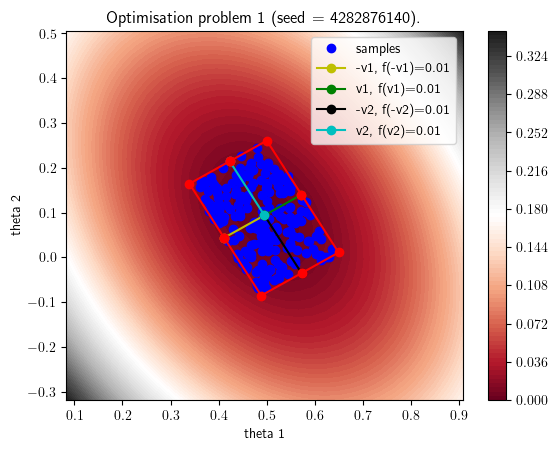
\includegraphics[width=0.49\textwidth]{./latex_files/images/chapter4/ma2_region_1.png}
        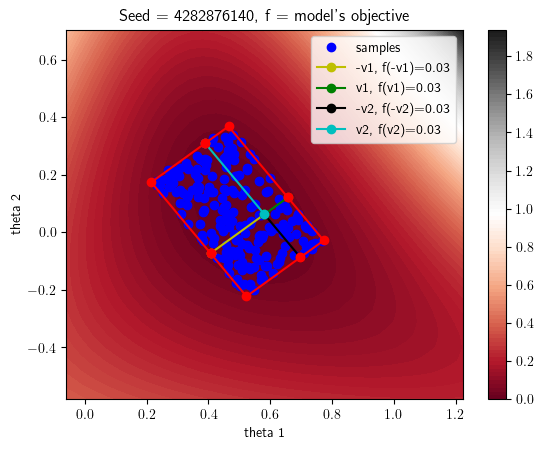
\includegraphics[width=0.49\textwidth]{./latex_files/images/chapter4/ma2_region_1_bo.png}
    \end{center}
  \caption[The acceptance region of a specific deterministic simulator.]{The acceptance region in a specific optimisation problem. In the left figure the region obtained with gradient-based optimiser and in the right one with Bayesian Optimisation.}
  \label{fig:ma2_5}
\end{figure}


\begin{figure}[ht]
  \begin{center}
    \resizebox{.24\columnwidth}{!}{%
      % This file was created with tikzplotlib v0.9.12.
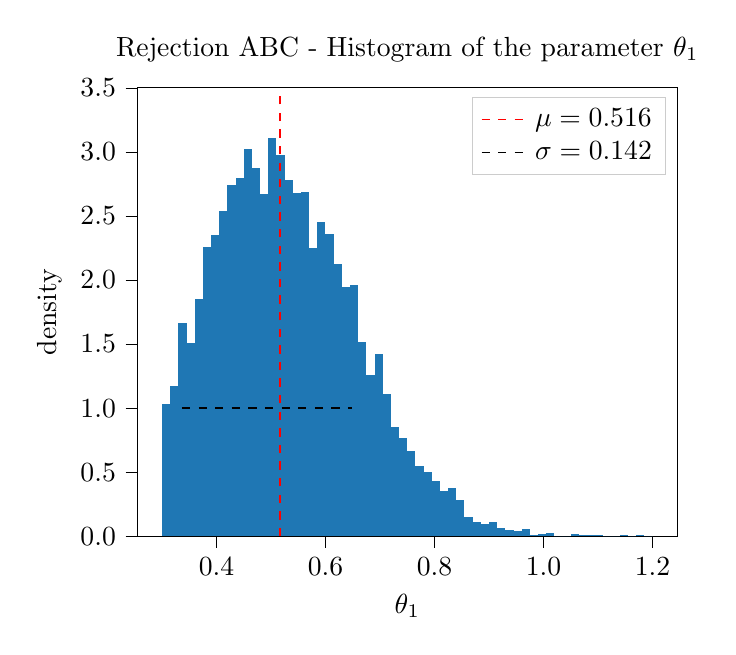
\begin{tikzpicture}

\definecolor{color0}{rgb}{0.12156862745098,0.466666666666667,0.705882352941177}

\begin{axis}[
legend cell align={left},
legend style={fill opacity=0.8, draw opacity=1, text opacity=1, draw=white!80!black},
tick align=outside,
tick pos=left,
title={Rejection ABC - Histogram of the parameter \(\displaystyle \theta_1\)},
x grid style={white!69.0196078431373!black},
xlabel={\(\displaystyle \theta_1\)},
xmin=0.255, xmax=1.245,
xtick style={color=black},
xtick={0.2,0.4,0.6,0.8,1,1.2,1.4},
xticklabels={
  \(\displaystyle {0.2}\),
  \(\displaystyle {0.4}\),
  \(\displaystyle {0.6}\),
  \(\displaystyle {0.8}\),
  \(\displaystyle {1.0}\),
  \(\displaystyle {1.2}\),
  \(\displaystyle {1.4}\)
},
y grid style={white!69.0196078431373!black},
ylabel={density},
ymin=0, ymax=3.5,
ytick style={color=black},
ytick={0,0.5,1,1.5,2,2.5,3,3.5},
yticklabels={
  \(\displaystyle {0.0}\),
  \(\displaystyle {0.5}\),
  \(\displaystyle {1.0}\),
  \(\displaystyle {1.5}\),
  \(\displaystyle {2.0}\),
  \(\displaystyle {2.5}\),
  \(\displaystyle {3.0}\),
  \(\displaystyle {3.5}\)
}
]
\draw[draw=none,fill=color0] (axis cs:0.3,0) rectangle (axis cs:0.315,1.02965548855742);
\draw[draw=none,fill=color0] (axis cs:0.315,0) rectangle (axis cs:0.33,1.17070418562009);
\draw[draw=none,fill=color0] (axis cs:0.33,0) rectangle (axis cs:0.345,1.6643746253394);
\draw[draw=none,fill=color0] (axis cs:0.345,0) rectangle (axis cs:0.36,1.50922105857047);
\draw[draw=none,fill=color0] (axis cs:0.36,0) rectangle (axis cs:0.375,1.85479036637399);
\draw[draw=none,fill=color0] (axis cs:0.375,0) rectangle (axis cs:0.39,2.25677915300258);
\draw[draw=none,fill=color0] (axis cs:0.39,0) rectangle (axis cs:0.405,2.3484608060933);
\draw[draw=none,fill=color0] (axis cs:0.405,0) rectangle (axis cs:0.42,2.53887654712789);
\draw[draw=none,fill=color0] (axis cs:0.42,0) rectangle (axis cs:0.435,2.74339715786876);
\draw[draw=none,fill=color0] (axis cs:0.435,0) rectangle (axis cs:0.45,2.79981663669382);
\draw[draw=none,fill=color0] (axis cs:0.45,0) rectangle (axis cs:0.465,3.02549455199407);
\draw[draw=none,fill=color0] (axis cs:0.465,0) rectangle (axis cs:0.48,2.87739342007828);
\draw[draw=none,fill=color0] (axis cs:0.48,0) rectangle (axis cs:0.495,2.67287280933742);
\draw[draw=none,fill=color0] (axis cs:0.495,0) rectangle (axis cs:0.51,3.11012377023167);
\draw[draw=none,fill=color0] (axis cs:0.51,0) rectangle (axis cs:0.525,2.97612750802216);
\draw[draw=none,fill=color0] (axis cs:0.525,0) rectangle (axis cs:0.54,2.77865933213442);
\draw[draw=none,fill=color0] (axis cs:0.54,0) rectangle (axis cs:0.555,2.67992524419055);
\draw[draw=none,fill=color0] (axis cs:0.555,0) rectangle (axis cs:0.57,2.68697767904369);
\draw[draw=none,fill=color0] (axis cs:0.57,0) rectangle (axis cs:0.585,2.24972671814944);
\draw[draw=none,fill=color0] (axis cs:0.585,0) rectangle (axis cs:0.6,2.45424732889032);
\draw[draw=none,fill=color0] (axis cs:0.6,0) rectangle (axis cs:0.615,2.35551324094642);
\draw[draw=none,fill=color0] (axis cs:0.615,0) rectangle (axis cs:0.63,2.12278289079306);
\draw[draw=none,fill=color0] (axis cs:0.63,0) rectangle (axis cs:0.645,1.9464720194647);
\draw[draw=none,fill=color0] (axis cs:0.645,0) rectangle (axis cs:0.66,1.960576889171);
\draw[draw=none,fill=color0] (axis cs:0.66,0) rectangle (axis cs:0.675,1.5162734934236);
\draw[draw=none,fill=color0] (axis cs:0.675,0) rectangle (axis cs:0.69,1.25533340385768);
\draw[draw=none,fill=color0] (axis cs:0.69,0) rectangle (axis cs:0.705,1.42459184033288);
\draw[draw=none,fill=color0] (axis cs:0.705,0) rectangle (axis cs:0.72,1.10723227194188);
\draw[draw=none,fill=color0] (axis cs:0.72,0) rectangle (axis cs:0.735,0.853344617229104);
\draw[draw=none,fill=color0] (axis cs:0.735,0) rectangle (axis cs:0.75,0.768715398991495);
\draw[draw=none,fill=color0] (axis cs:0.75,0) rectangle (axis cs:0.765,0.66292887619451);
\draw[draw=none,fill=color0] (axis cs:0.765,0) rectangle (axis cs:0.78,0.550089918544377);
\draw[draw=none,fill=color0] (axis cs:0.78,0) rectangle (axis cs:0.795,0.500722874572446);
\draw[draw=none,fill=color0] (axis cs:0.795,0) rectangle (axis cs:0.81,0.430198526041119);
\draw[draw=none,fill=color0] (axis cs:0.81,0) rectangle (axis cs:0.825,0.352621742656649);
\draw[draw=none,fill=color0] (axis cs:0.825,0) rectangle (axis cs:0.84,0.373779047216054);
\draw[draw=none,fill=color0] (axis cs:0.84,0) rectangle (axis cs:0.855,0.282097394125319);
\draw[draw=none,fill=color0] (axis cs:0.855,0) rectangle (axis cs:0.87,0.148101131915795);
\draw[draw=none,fill=color0] (axis cs:0.87,0) rectangle (axis cs:0.885,0.112838957650128);
\draw[draw=none,fill=color0] (axis cs:0.885,0) rectangle (axis cs:0.9,0.0916816530907302);
\draw[draw=none,fill=color0] (axis cs:0.9,0) rectangle (axis cs:0.915,0.112838957650129);
\draw[draw=none,fill=color0] (axis cs:0.915,0) rectangle (axis cs:0.93,0.0634719136781969);
\draw[draw=none,fill=color0] (axis cs:0.93,0) rectangle (axis cs:0.945,0.0493670439719316);
\draw[draw=none,fill=color0] (axis cs:0.945,0) rectangle (axis cs:0.96,0.0423146091187979);
\draw[draw=none,fill=color0] (axis cs:0.96,0) rectangle (axis cs:0.975,0.0564194788250647);
\draw[draw=none,fill=color0] (axis cs:0.975,0) rectangle (axis cs:0.99,0.00705243485313299);
\draw[draw=none,fill=color0] (axis cs:0.99,0) rectangle (axis cs:1.005,0.0141048697062662);
\draw[draw=none,fill=color0] (axis cs:1.005,0) rectangle (axis cs:1.02,0.0282097394125324);
\draw[draw=none,fill=color0] (axis cs:1.02,0) rectangle (axis cs:1.035,0);
\draw[draw=none,fill=color0] (axis cs:1.035,0) rectangle (axis cs:1.05,0);
\draw[draw=none,fill=color0] (axis cs:1.05,0) rectangle (axis cs:1.065,0.014104869706266);
\draw[draw=none,fill=color0] (axis cs:1.065,0) rectangle (axis cs:1.08,0.00705243485313309);
\draw[draw=none,fill=color0] (axis cs:1.08,0) rectangle (axis cs:1.095,0.00705243485313299);
\draw[draw=none,fill=color0] (axis cs:1.095,0) rectangle (axis cs:1.11,0.00705243485313309);
\draw[draw=none,fill=color0] (axis cs:1.11,0) rectangle (axis cs:1.125,0);
\draw[draw=none,fill=color0] (axis cs:1.125,0) rectangle (axis cs:1.14,0);
\draw[draw=none,fill=color0] (axis cs:1.14,0) rectangle (axis cs:1.155,0.00705243485313309);
\draw[draw=none,fill=color0] (axis cs:1.155,0) rectangle (axis cs:1.17,0);
\draw[draw=none,fill=color0] (axis cs:1.17,0) rectangle (axis cs:1.185,0.00705243485313309);
\draw[draw=none,fill=color0] (axis cs:1.185,0) rectangle (axis cs:1.2,0);
\addplot [semithick, red, dashed]
table {%
0.51592730438119 0
0.51592730438119 3.5
};
\addlegendentry{$\mu = 0.516$}
\addplot [semithick, black, dashed]
table {%
0.336596813861936 1
0.648443255776683 1
};
\addlegendentry{$\sigma = 0.142$}
\end{axis}

\end{tikzpicture}

    }
    \resizebox{.24\columnwidth}{!}{%
      % This file was created by tikzplotlib v0.9.9.
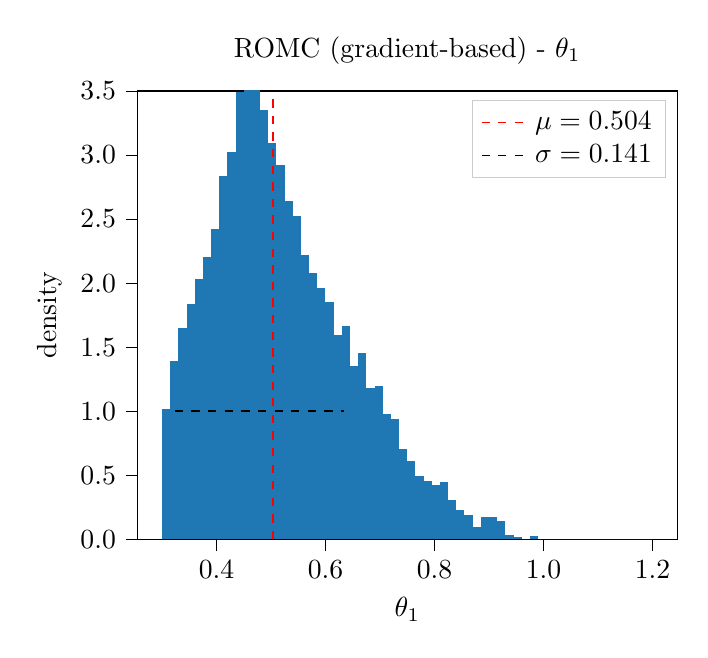
\begin{tikzpicture}

\definecolor{color0}{rgb}{0.12156862745098,0.466666666666667,0.705882352941177}

\begin{axis}[
legend cell align={left},
legend style={fill opacity=0.8, draw opacity=1, text opacity=1, draw=white!80!black},
tick align=outside,
tick pos=left,
title={ROMC (gradient-based) - \(\displaystyle \theta_1\)},
x grid style={white!69.0196078431373!black},
xlabel={\(\displaystyle \theta_1\)},
xmin=0.255, xmax=1.245,
xtick style={color=black},
xtick={0.2,0.4,0.6,0.8,1,1.2,1.4},
xticklabels={
  \(\displaystyle {0.2}\),
  \(\displaystyle {0.4}\),
  \(\displaystyle {0.6}\),
  \(\displaystyle {0.8}\),
  \(\displaystyle {1.0}\),
  \(\displaystyle {1.2}\),
  \(\displaystyle {1.4}\)
},
y grid style={white!69.0196078431373!black},
ylabel={density},
ymin=0, ymax=3.5,
ytick style={color=black},
ytick={0,0.5,1,1.5,2,2.5,3,3.5},
yticklabels={
  \(\displaystyle {0.0}\),
  \(\displaystyle {0.5}\),
  \(\displaystyle {1.0}\),
  \(\displaystyle {1.5}\),
  \(\displaystyle {2.0}\),
  \(\displaystyle {2.5}\),
  \(\displaystyle {3.0}\),
  \(\displaystyle {3.5}\)
}
]
\draw[draw=none,fill=color0] (axis cs:0.3,0) rectangle (axis cs:0.315,1.02018167274615);
\draw[draw=none,fill=color0] (axis cs:0.315,0) rectangle (axis cs:0.33,1.39039538321726);
\draw[draw=none,fill=color0] (axis cs:0.33,0) rectangle (axis cs:0.345,1.64837235793467);
\draw[draw=none,fill=color0] (axis cs:0.345,0) rectangle (axis cs:0.36,1.83766715107148);
\draw[draw=none,fill=color0] (axis cs:0.36,0) rectangle (axis cs:0.375,2.03114988210955);
\draw[draw=none,fill=color0] (axis cs:0.375,0) rectangle (axis cs:0.39,2.20118016090059);
\draw[draw=none,fill=color0] (axis cs:0.39,0) rectangle (axis cs:0.405,2.42565363240795);
\draw[draw=none,fill=color0] (axis cs:0.405,0) rectangle (axis cs:0.42,2.83858430947187);
\draw[draw=none,fill=color0] (axis cs:0.42,0) rectangle (axis cs:0.435,3.02313277298727);
\draw[draw=none,fill=color0] (axis cs:0.435,0) rectangle (axis cs:0.45,3.49050664276752);
\draw[draw=none,fill=color0] (axis cs:0.45,0) rectangle (axis cs:0.465,3.58012851385441);
\draw[draw=none,fill=color0] (axis cs:0.465,0) rectangle (axis cs:0.48,3.63066296452957);
\draw[draw=none,fill=color0] (axis cs:0.48,0) rectangle (axis cs:0.495,3.34895434170502);
\draw[draw=none,fill=color0] (axis cs:0.495,0) rectangle (axis cs:0.51,3.09544450074894);
\draw[draw=none,fill=color0] (axis cs:0.51,0) rectangle (axis cs:0.525,2.92569341781802);
\draw[draw=none,fill=color0] (axis cs:0.525,0) rectangle (axis cs:0.54,2.63923846537203);
\draw[draw=none,fill=color0] (axis cs:0.54,0) rectangle (axis cs:0.555,2.52616414203809);
\draw[draw=none,fill=color0] (axis cs:0.555,0) rectangle (axis cs:0.57,2.21569834562492);
\draw[draw=none,fill=color0] (axis cs:0.57,0) rectangle (axis cs:0.585,2.07749639488345);
\draw[draw=none,fill=color0] (axis cs:0.585,0) rectangle (axis cs:0.6,1.95995493778819);
\draw[draw=none,fill=color0] (axis cs:0.6,0) rectangle (axis cs:0.615,1.85302292337607);
\draw[draw=none,fill=color0] (axis cs:0.615,0) rectangle (axis cs:0.63,1.59560434037885);
\draw[draw=none,fill=color0] (axis cs:0.63,0) rectangle (axis cs:0.645,1.66428652195943);
\draw[draw=none,fill=color0] (axis cs:0.645,0) rectangle (axis cs:0.66,1.3535415296862);
\draw[draw=none,fill=color0] (axis cs:0.66,0) rectangle (axis cs:0.675,1.45042249313527);
\draw[draw=none,fill=color0] (axis cs:0.675,0) rectangle (axis cs:0.69,1.1846280343355);
\draw[draw=none,fill=color0] (axis cs:0.69,0) rectangle (axis cs:0.705,1.19830863147962);
\draw[draw=none,fill=color0] (axis cs:0.705,0) rectangle (axis cs:0.72,0.979977468894081);
\draw[draw=none,fill=color0] (axis cs:0.72,0) rectangle (axis cs:0.735,0.941727636062617);
\draw[draw=none,fill=color0] (axis cs:0.735,0) rectangle (axis cs:0.75,0.705807134291806);
\draw[draw=none,fill=color0] (axis cs:0.75,0) rectangle (axis cs:0.765,0.614789283904501);
\draw[draw=none,fill=color0] (axis cs:0.765,0) rectangle (axis cs:0.78,0.496689435089055);
\draw[draw=none,fill=color0] (axis cs:0.78,0) rectangle (axis cs:0.795,0.456206035376906);
\draw[draw=none,fill=color0] (axis cs:0.795,0) rectangle (axis cs:0.81,0.425773686627776);
\draw[draw=none,fill=color0] (axis cs:0.81,0) rectangle (axis cs:0.825,0.449226138874808);
\draw[draw=none,fill=color0] (axis cs:0.825,0) rectangle (axis cs:0.84,0.309907404693004);
\draw[draw=none,fill=color0] (axis cs:0.84,0) rectangle (axis cs:0.855,0.224752667367446);
\draw[draw=none,fill=color0] (axis cs:0.855,0) rectangle (axis cs:0.87,0.192924339317897);
\draw[draw=none,fill=color0] (axis cs:0.87,0) rectangle (axis cs:0.885,0.0974393551692405);
\draw[draw=none,fill=color0] (axis cs:0.885,0) rectangle (axis cs:0.9,0.176730979433038);
\draw[draw=none,fill=color0] (axis cs:0.9,0) rectangle (axis cs:0.915,0.170309474651111);
\draw[draw=none,fill=color0] (axis cs:0.915,0) rectangle (axis cs:0.93,0.145461043103651);
\draw[draw=none,fill=color0] (axis cs:0.93,0) rectangle (axis cs:0.945,0.0304323487491329);
\draw[draw=none,fill=color0] (axis cs:0.945,0) rectangle (axis cs:0.96,0.0206604936462);
\draw[draw=none,fill=color0] (axis cs:0.96,0) rectangle (axis cs:0.975,0);
\draw[draw=none,fill=color0] (axis cs:0.975,0) rectangle (axis cs:0.99,0.0217772770865351);
\draw[draw=none,fill=color0] (axis cs:0.99,0) rectangle (axis cs:1.005,0);
\draw[draw=none,fill=color0] (axis cs:1.005,0) rectangle (axis cs:1.02,0);
\draw[draw=none,fill=color0] (axis cs:1.02,0) rectangle (axis cs:1.035,0);
\draw[draw=none,fill=color0] (axis cs:1.035,0) rectangle (axis cs:1.05,0);
\draw[draw=none,fill=color0] (axis cs:1.05,0) rectangle (axis cs:1.065,0);
\draw[draw=none,fill=color0] (axis cs:1.065,0) rectangle (axis cs:1.08,0);
\draw[draw=none,fill=color0] (axis cs:1.08,0) rectangle (axis cs:1.095,0);
\draw[draw=none,fill=color0] (axis cs:1.095,0) rectangle (axis cs:1.11,0);
\draw[draw=none,fill=color0] (axis cs:1.11,0) rectangle (axis cs:1.125,0);
\draw[draw=none,fill=color0] (axis cs:1.125,0) rectangle (axis cs:1.14,0);
\draw[draw=none,fill=color0] (axis cs:1.14,0) rectangle (axis cs:1.155,0);
\draw[draw=none,fill=color0] (axis cs:1.155,0) rectangle (axis cs:1.17,0);
\draw[draw=none,fill=color0] (axis cs:1.17,0) rectangle (axis cs:1.185,0);
\draw[draw=none,fill=color0] (axis cs:1.185,0) rectangle (axis cs:1.2,0);
\addplot [semithick, red, dashed]
table {%
0.503688298846839 0
0.503688298846839 3.5
};
\addlegendentry{$\mu = 0.504$}
\addplot [semithick, black, dashed]
table {%
0.323676768279387 1
0.634437489183658 1
};
\addlegendentry{$\sigma = 0.141$}
\end{axis}

\end{tikzpicture}

    }
    \resizebox{.24\columnwidth}{!}{%
      % This file was created by tikzplotlib v0.9.9.
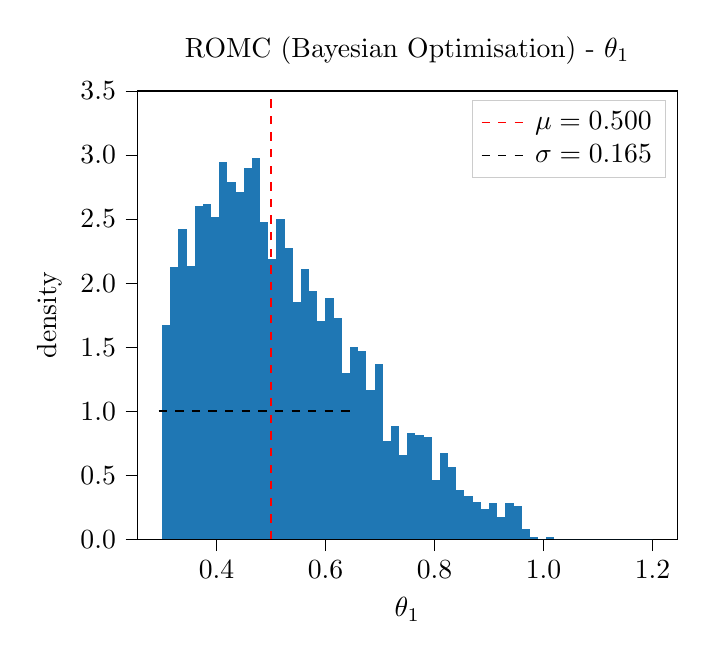
\begin{tikzpicture}

\definecolor{color0}{rgb}{0.12156862745098,0.466666666666667,0.705882352941177}

\begin{axis}[
legend cell align={left},
legend style={fill opacity=0.8, draw opacity=1, text opacity=1, draw=white!80!black},
tick align=outside,
tick pos=left,
title={ROMC (Bayesian Optimisation) - \(\displaystyle \theta_1\)},
x grid style={white!69.0196078431373!black},
xlabel={\(\displaystyle \theta_1\)},
xmin=0.255, xmax=1.245,
xtick style={color=black},
xtick={0.2,0.4,0.6,0.8,1,1.2,1.4},
xticklabels={
  \(\displaystyle {0.2}\),
  \(\displaystyle {0.4}\),
  \(\displaystyle {0.6}\),
  \(\displaystyle {0.8}\),
  \(\displaystyle {1.0}\),
  \(\displaystyle {1.2}\),
  \(\displaystyle {1.4}\)
},
y grid style={white!69.0196078431373!black},
ylabel={density},
ymin=0, ymax=3.5,
ytick style={color=black},
ytick={0,0.5,1,1.5,2,2.5,3,3.5},
yticklabels={
  \(\displaystyle {0.0}\),
  \(\displaystyle {0.5}\),
  \(\displaystyle {1.0}\),
  \(\displaystyle {1.5}\),
  \(\displaystyle {2.0}\),
  \(\displaystyle {2.5}\),
  \(\displaystyle {3.0}\),
  \(\displaystyle {3.5}\)
}
]
\draw[draw=none,fill=color0] (axis cs:0.3,0) rectangle (axis cs:0.315,1.67339010906917);
\draw[draw=none,fill=color0] (axis cs:0.315,0) rectangle (axis cs:0.33,2.12285439456296);
\draw[draw=none,fill=color0] (axis cs:0.33,0) rectangle (axis cs:0.345,2.41994534810638);
\draw[draw=none,fill=color0] (axis cs:0.345,0) rectangle (axis cs:0.36,2.13421448089961);
\draw[draw=none,fill=color0] (axis cs:0.36,0) rectangle (axis cs:0.375,2.60269456308737);
\draw[draw=none,fill=color0] (axis cs:0.375,0) rectangle (axis cs:0.39,2.61479552461991);
\draw[draw=none,fill=color0] (axis cs:0.39,0) rectangle (axis cs:0.405,2.51971654115006);
\draw[draw=none,fill=color0] (axis cs:0.405,0) rectangle (axis cs:0.42,2.94571977877467);
\draw[draw=none,fill=color0] (axis cs:0.42,0) rectangle (axis cs:0.435,2.78840727885186);
\draw[draw=none,fill=color0] (axis cs:0.435,0) rectangle (axis cs:0.45,2.70814579929938);
\draw[draw=none,fill=color0] (axis cs:0.45,0) rectangle (axis cs:0.465,2.89534026545558);
\draw[draw=none,fill=color0] (axis cs:0.465,0) rectangle (axis cs:0.48,2.97807132899427);
\draw[draw=none,fill=color0] (axis cs:0.48,0) rectangle (axis cs:0.495,2.47304140381032);
\draw[draw=none,fill=color0] (axis cs:0.495,0) rectangle (axis cs:0.51,2.18508791101595);
\draw[draw=none,fill=color0] (axis cs:0.51,0) rectangle (axis cs:0.525,2.50193553644923);
\draw[draw=none,fill=color0] (axis cs:0.525,0) rectangle (axis cs:0.54,2.27646251850645);
\draw[draw=none,fill=color0] (axis cs:0.54,0) rectangle (axis cs:0.555,1.84996536408459);
\draw[draw=none,fill=color0] (axis cs:0.555,0) rectangle (axis cs:0.57,2.10951864103732);
\draw[draw=none,fill=color0] (axis cs:0.57,0) rectangle (axis cs:0.585,1.94010517958197);
\draw[draw=none,fill=color0] (axis cs:0.585,0) rectangle (axis cs:0.6,1.70154336651221);
\draw[draw=none,fill=color0] (axis cs:0.6,0) rectangle (axis cs:0.615,1.88058820551382);
\draw[draw=none,fill=color0] (axis cs:0.615,0) rectangle (axis cs:0.63,1.72549833117864);
\draw[draw=none,fill=color0] (axis cs:0.63,0) rectangle (axis cs:0.645,1.29579071757466);
\draw[draw=none,fill=color0] (axis cs:0.645,0) rectangle (axis cs:0.66,1.50076618843174);
\draw[draw=none,fill=color0] (axis cs:0.66,0) rectangle (axis cs:0.675,1.46940247180661);
\draw[draw=none,fill=color0] (axis cs:0.675,0) rectangle (axis cs:0.69,1.16860714228384);
\draw[draw=none,fill=color0] (axis cs:0.69,0) rectangle (axis cs:0.705,1.37012519556019);
\draw[draw=none,fill=color0] (axis cs:0.705,0) rectangle (axis cs:0.72,0.767793661318775);
\draw[draw=none,fill=color0] (axis cs:0.72,0) rectangle (axis cs:0.735,0.885098900664694);
\draw[draw=none,fill=color0] (axis cs:0.735,0) rectangle (axis cs:0.75,0.65715629873569);
\draw[draw=none,fill=color0] (axis cs:0.75,0) rectangle (axis cs:0.765,0.82731063538692);
\draw[draw=none,fill=color0] (axis cs:0.765,0) rectangle (axis cs:0.78,0.813727923462651);
\draw[draw=none,fill=color0] (axis cs:0.78,0) rectangle (axis cs:0.795,0.801873920328749);
\draw[draw=none,fill=color0] (axis cs:0.795,0) rectangle (axis cs:0.81,0.459095663040085);
\draw[draw=none,fill=color0] (axis cs:0.81,0) rectangle (axis cs:0.825,0.672961636247559);
\draw[draw=none,fill=color0] (axis cs:0.825,0) rectangle (axis cs:0.84,0.561583398468614);
\draw[draw=none,fill=color0] (axis cs:0.84,0) rectangle (axis cs:0.855,0.382538559466961);
\draw[draw=none,fill=color0] (axis cs:0.855,0) rectangle (axis cs:0.87,0.340555631701063);
\draw[draw=none,fill=color0] (axis cs:0.87,0) rectangle (axis cs:0.885,0.294127452759942);
\draw[draw=none,fill=color0] (axis cs:0.885,0) rectangle (axis cs:0.9,0.239055729867026);
\draw[draw=none,fill=color0] (axis cs:0.9,0) rectangle (axis cs:0.915,0.283755200017783);
\draw[draw=none,fill=color0] (axis cs:0.915,0) rectangle (axis cs:0.93,0.176575255015415);
\draw[draw=none,fill=color0] (axis cs:0.93,0) rectangle (axis cs:0.945,0.283261283220537);
\draw[draw=none,fill=color0] (axis cs:0.945,0) rectangle (axis cs:0.96,0.258071526560991);
\draw[draw=none,fill=color0] (axis cs:0.96,0) rectangle (axis cs:0.975,0.0775449371676099);
\draw[draw=none,fill=color0] (axis cs:0.975,0) rectangle (axis cs:0.99,0.0155583791132463);
\draw[draw=none,fill=color0] (axis cs:0.99,0) rectangle (axis cs:1.005,0);
\draw[draw=none,fill=color0] (axis cs:1.005,0) rectangle (axis cs:1.02,0.0172870879036073);
\draw[draw=none,fill=color0] (axis cs:1.02,0) rectangle (axis cs:1.035,0);
\draw[draw=none,fill=color0] (axis cs:1.035,0) rectangle (axis cs:1.05,0);
\draw[draw=none,fill=color0] (axis cs:1.05,0) rectangle (axis cs:1.065,0);
\draw[draw=none,fill=color0] (axis cs:1.065,0) rectangle (axis cs:1.08,0);
\draw[draw=none,fill=color0] (axis cs:1.08,0) rectangle (axis cs:1.095,0);
\draw[draw=none,fill=color0] (axis cs:1.095,0) rectangle (axis cs:1.11,0);
\draw[draw=none,fill=color0] (axis cs:1.11,0) rectangle (axis cs:1.125,0);
\draw[draw=none,fill=color0] (axis cs:1.125,0) rectangle (axis cs:1.14,0);
\draw[draw=none,fill=color0] (axis cs:1.14,0) rectangle (axis cs:1.155,0);
\draw[draw=none,fill=color0] (axis cs:1.155,0) rectangle (axis cs:1.17,0);
\draw[draw=none,fill=color0] (axis cs:1.17,0) rectangle (axis cs:1.185,0);
\draw[draw=none,fill=color0] (axis cs:1.185,0) rectangle (axis cs:1.2,0);
\addplot [semithick, red, dashed]
table {%
0.500240536632723 0
0.500240536632723 3.5
};
\addlegendentry{$\mu = 0.500$}
\addplot [semithick, black, dashed]
table {%
0.293929386789429 1
0.656599793802562 1
};
\addlegendentry{$\sigma = 0.165$}
\end{axis}

\end{tikzpicture}

    }
    \resizebox{.24\columnwidth}{!}{%
      % This file was created with tikzplotlib v0.9.12.
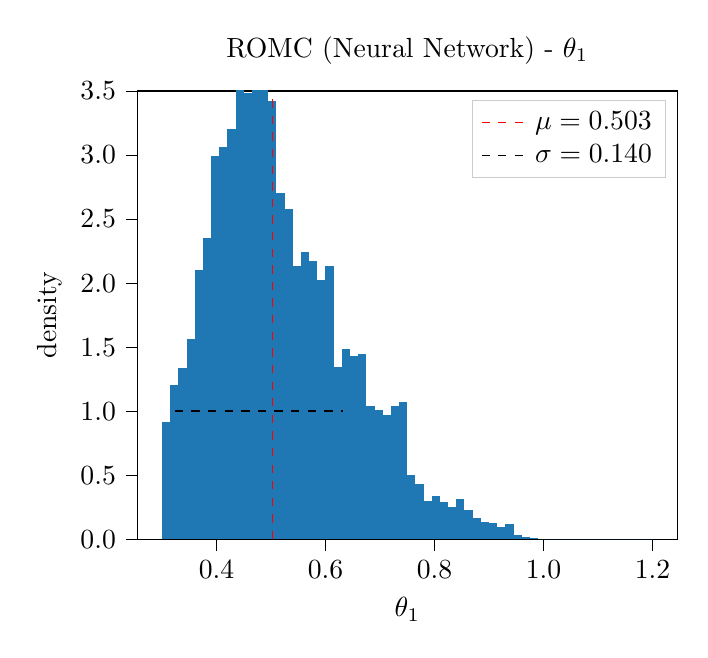
\begin{tikzpicture}

\definecolor{color0}{rgb}{0.12156862745098,0.466666666666667,0.705882352941177}

\begin{axis}[
legend cell align={left},
legend style={fill opacity=0.8, draw opacity=1, text opacity=1, draw=white!80!black},
tick align=outside,
tick pos=left,
title={ROMC (Neural Network) - \(\displaystyle \theta_1\)},
x grid style={white!69.0196078431373!black},
xlabel={\(\displaystyle \theta_1\)},
xmin=0.255, xmax=1.245,
xtick style={color=black},
xtick={0.2,0.4,0.6,0.8,1,1.2,1.4},
xticklabels={
  \(\displaystyle {0.2}\),
  \(\displaystyle {0.4}\),
  \(\displaystyle {0.6}\),
  \(\displaystyle {0.8}\),
  \(\displaystyle {1.0}\),
  \(\displaystyle {1.2}\),
  \(\displaystyle {1.4}\)
},
y grid style={white!69.0196078431373!black},
ylabel={density},
ymin=0, ymax=3.5,
ytick style={color=black},
ytick={0,0.5,1,1.5,2,2.5,3,3.5},
yticklabels={
  \(\displaystyle {0.0}\),
  \(\displaystyle {0.5}\),
  \(\displaystyle {1.0}\),
  \(\displaystyle {1.5}\),
  \(\displaystyle {2.0}\),
  \(\displaystyle {2.5}\),
  \(\displaystyle {3.0}\),
  \(\displaystyle {3.5}\)
}
]
\draw[draw=none,fill=color0] (axis cs:0.3,0) rectangle (axis cs:0.315,0.918657455133441);
\draw[draw=none,fill=color0] (axis cs:0.315,0) rectangle (axis cs:0.33,1.20251419656731);
\draw[draw=none,fill=color0] (axis cs:0.33,0) rectangle (axis cs:0.345,1.33742778487049);
\draw[draw=none,fill=color0] (axis cs:0.345,0) rectangle (axis cs:0.36,1.56194622164953);
\draw[draw=none,fill=color0] (axis cs:0.36,0) rectangle (axis cs:0.375,2.10132928493464);
\draw[draw=none,fill=color0] (axis cs:0.375,0) rectangle (axis cs:0.39,2.35262182295654);
\draw[draw=none,fill=color0] (axis cs:0.39,0) rectangle (axis cs:0.405,2.99077324408847);
\draw[draw=none,fill=color0] (axis cs:0.405,0) rectangle (axis cs:0.42,3.06195916743878);
\draw[draw=none,fill=color0] (axis cs:0.42,0) rectangle (axis cs:0.435,3.20534143070652);
\draw[draw=none,fill=color0] (axis cs:0.435,0) rectangle (axis cs:0.45,3.54249833812081);
\draw[draw=none,fill=color0] (axis cs:0.45,0) rectangle (axis cs:0.465,3.48746191660371);
\draw[draw=none,fill=color0] (axis cs:0.465,0) rectangle (axis cs:0.48,3.64921604449934);
\draw[draw=none,fill=color0] (axis cs:0.48,0) rectangle (axis cs:0.495,3.65237906359403);
\draw[draw=none,fill=color0] (axis cs:0.495,0) rectangle (axis cs:0.51,3.41841807637564);
\draw[draw=none,fill=color0] (axis cs:0.51,0) rectangle (axis cs:0.525,2.70295622336452);
\draw[draw=none,fill=color0] (axis cs:0.525,0) rectangle (axis cs:0.54,2.57664640133676);
\draw[draw=none,fill=color0] (axis cs:0.54,0) rectangle (axis cs:0.555,2.13473725538676);
\draw[draw=none,fill=color0] (axis cs:0.555,0) rectangle (axis cs:0.57,2.24111391157059);
\draw[draw=none,fill=color0] (axis cs:0.57,0) rectangle (axis cs:0.585,2.17436219440432);
\draw[draw=none,fill=color0] (axis cs:0.585,0) rectangle (axis cs:0.6,2.02392362475434);
\draw[draw=none,fill=color0] (axis cs:0.6,0) rectangle (axis cs:0.615,2.1307420959631);
\draw[draw=none,fill=color0] (axis cs:0.615,0) rectangle (axis cs:0.63,1.34480742455423);
\draw[draw=none,fill=color0] (axis cs:0.63,0) rectangle (axis cs:0.645,1.48585437983289);
\draw[draw=none,fill=color0] (axis cs:0.645,0) rectangle (axis cs:0.66,1.43000242757426);
\draw[draw=none,fill=color0] (axis cs:0.66,0) rectangle (axis cs:0.675,1.44793856735925);
\draw[draw=none,fill=color0] (axis cs:0.675,0) rectangle (axis cs:0.69,1.04402163798497);
\draw[draw=none,fill=color0] (axis cs:0.69,0) rectangle (axis cs:0.705,1.00795945546565);
\draw[draw=none,fill=color0] (axis cs:0.705,0) rectangle (axis cs:0.72,0.973472415485145);
\draw[draw=none,fill=color0] (axis cs:0.72,0) rectangle (axis cs:0.735,1.03878684968805);
\draw[draw=none,fill=color0] (axis cs:0.735,0) rectangle (axis cs:0.75,1.07033952922709);
\draw[draw=none,fill=color0] (axis cs:0.75,0) rectangle (axis cs:0.765,0.499611406245489);
\draw[draw=none,fill=color0] (axis cs:0.765,0) rectangle (axis cs:0.78,0.427526350563684);
\draw[draw=none,fill=color0] (axis cs:0.78,0) rectangle (axis cs:0.795,0.301712601546415);
\draw[draw=none,fill=color0] (axis cs:0.795,0) rectangle (axis cs:0.81,0.33618635385698);
\draw[draw=none,fill=color0] (axis cs:0.81,0) rectangle (axis cs:0.825,0.291403030644556);
\draw[draw=none,fill=color0] (axis cs:0.825,0) rectangle (axis cs:0.84,0.251052806310352);
\draw[draw=none,fill=color0] (axis cs:0.84,0) rectangle (axis cs:0.855,0.313679809271219);
\draw[draw=none,fill=color0] (axis cs:0.855,0) rectangle (axis cs:0.87,0.230501210162083);
\draw[draw=none,fill=color0] (axis cs:0.87,0) rectangle (axis cs:0.885,0.16371073729186);
\draw[draw=none,fill=color0] (axis cs:0.885,0) rectangle (axis cs:0.9,0.133740397779522);
\draw[draw=none,fill=color0] (axis cs:0.9,0) rectangle (axis cs:0.915,0.128624644858993);
\draw[draw=none,fill=color0] (axis cs:0.915,0) rectangle (axis cs:0.93,0.097498278063311);
\draw[draw=none,fill=color0] (axis cs:0.93,0) rectangle (axis cs:0.945,0.119954440233943);
\draw[draw=none,fill=color0] (axis cs:0.945,0) rectangle (axis cs:0.96,0.0362421197162086);
\draw[draw=none,fill=color0] (axis cs:0.96,0) rectangle (axis cs:0.975,0.0137859575455791);
\draw[draw=none,fill=color0] (axis cs:0.975,0) rectangle (axis cs:0.99,0.0112280810853149);
\draw[draw=none,fill=color0] (axis cs:0.99,0) rectangle (axis cs:1.005,0);
\draw[draw=none,fill=color0] (axis cs:1.005,0) rectangle (axis cs:1.02,0);
\draw[draw=none,fill=color0] (axis cs:1.02,0) rectangle (axis cs:1.035,0);
\draw[draw=none,fill=color0] (axis cs:1.035,0) rectangle (axis cs:1.05,0);
\draw[draw=none,fill=color0] (axis cs:1.05,0) rectangle (axis cs:1.065,0);
\draw[draw=none,fill=color0] (axis cs:1.065,0) rectangle (axis cs:1.08,0);
\draw[draw=none,fill=color0] (axis cs:1.08,0) rectangle (axis cs:1.095,0);
\draw[draw=none,fill=color0] (axis cs:1.095,0) rectangle (axis cs:1.11,0);
\draw[draw=none,fill=color0] (axis cs:1.11,0) rectangle (axis cs:1.125,0);
\draw[draw=none,fill=color0] (axis cs:1.125,0) rectangle (axis cs:1.14,0);
\draw[draw=none,fill=color0] (axis cs:1.14,0) rectangle (axis cs:1.155,0);
\draw[draw=none,fill=color0] (axis cs:1.155,0) rectangle (axis cs:1.17,0);
\draw[draw=none,fill=color0] (axis cs:1.17,0) rectangle (axis cs:1.185,0);
\draw[draw=none,fill=color0] (axis cs:1.185,0) rectangle (axis cs:1.2,0);
\addplot [semithick, red, dashed]
table {%
0.502656907372089 0
0.502656907372089 3.5
};
\addlegendentry{$\mu = 0.503$}
\addplot [semithick, black, dashed]
table {%
0.32355294654317 1
0.632292249675427 1
};
\addlegendentry{$\sigma = 0.140$}
\end{axis}

\end{tikzpicture}

    }\\
    \resizebox{.24\columnwidth}{!}{%
      % This file was created with tikzplotlib v0.9.12.
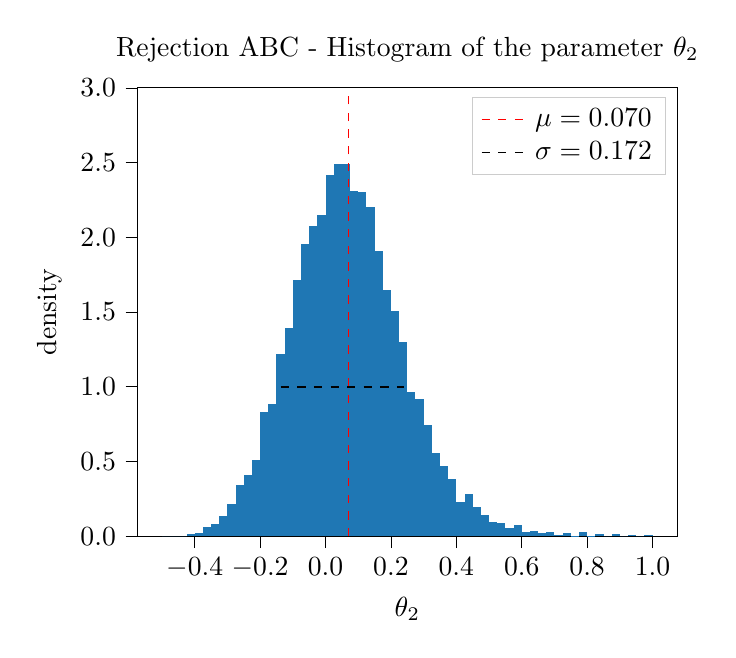
\begin{tikzpicture}

\definecolor{color0}{rgb}{0.12156862745098,0.466666666666667,0.705882352941177}

\begin{axis}[
legend cell align={left},
legend style={fill opacity=0.8, draw opacity=1, text opacity=1, draw=white!80!black},
tick align=outside,
tick pos=left,
title={Rejection ABC - Histogram of the parameter \(\displaystyle \theta_2\)},
x grid style={white!69.0196078431373!black},
xlabel={\(\displaystyle \theta_2\)},
xmin=-0.575, xmax=1.075,
xtick style={color=black},
xtick={-0.6,-0.4,-0.2,0,0.2,0.4,0.6,0.8,1,1.2},
xticklabels={
  \(\displaystyle {\ensuremath{-}0.6}\),
  \(\displaystyle {\ensuremath{-}0.4}\),
  \(\displaystyle {\ensuremath{-}0.2}\),
  \(\displaystyle {0.0}\),
  \(\displaystyle {0.2}\),
  \(\displaystyle {0.4}\),
  \(\displaystyle {0.6}\),
  \(\displaystyle {0.8}\),
  \(\displaystyle {1.0}\),
  \(\displaystyle {1.2}\)
},
y grid style={white!69.0196078431373!black},
ylabel={density},
ymin=0, ymax=3,
ytick style={color=black},
ytick={0,0.5,1,1.5,2,2.5,3},
yticklabels={
  \(\displaystyle {0.0}\),
  \(\displaystyle {0.5}\),
  \(\displaystyle {1.0}\),
  \(\displaystyle {1.5}\),
  \(\displaystyle {2.0}\),
  \(\displaystyle {2.5}\),
  \(\displaystyle {3.0}\)
}
]
\draw[draw=none,fill=color0] (axis cs:-0.5,0) rectangle (axis cs:-0.475,0);
\draw[draw=none,fill=color0] (axis cs:-0.475,0) rectangle (axis cs:-0.45,0);
\draw[draw=none,fill=color0] (axis cs:-0.45,0) rectangle (axis cs:-0.425,0);
\draw[draw=none,fill=color0] (axis cs:-0.425,0) rectangle (axis cs:-0.4,0.016001600160016);
\draw[draw=none,fill=color0] (axis cs:-0.4,0) rectangle (axis cs:-0.375,0.02000200020002);
\draw[draw=none,fill=color0] (axis cs:-0.375,0) rectangle (axis cs:-0.35,0.0600060006000599);
\draw[draw=none,fill=color0] (axis cs:-0.35,0) rectangle (axis cs:-0.325,0.0800080008000799);
\draw[draw=none,fill=color0] (axis cs:-0.325,0) rectangle (axis cs:-0.3,0.132013201320132);
\draw[draw=none,fill=color0] (axis cs:-0.3,0) rectangle (axis cs:-0.275,0.216021602160216);
\draw[draw=none,fill=color0] (axis cs:-0.275,0) rectangle (axis cs:-0.25,0.344034403440344);
\draw[draw=none,fill=color0] (axis cs:-0.25,0) rectangle (axis cs:-0.225,0.412041204120412);
\draw[draw=none,fill=color0] (axis cs:-0.225,0) rectangle (axis cs:-0.2,0.508050805080508);
\draw[draw=none,fill=color0] (axis cs:-0.2,0) rectangle (axis cs:-0.175,0.832083208320833);
\draw[draw=none,fill=color0] (axis cs:-0.175,0) rectangle (axis cs:-0.15,0.884088408840883);
\draw[draw=none,fill=color0] (axis cs:-0.15,0) rectangle (axis cs:-0.125,1.21612161216122);
\draw[draw=none,fill=color0] (axis cs:-0.125,0) rectangle (axis cs:-0.1,1.39213921392139);
\draw[draw=none,fill=color0] (axis cs:-0.1,0) rectangle (axis cs:-0.075,1.71217121712171);
\draw[draw=none,fill=color0] (axis cs:-0.075,0) rectangle (axis cs:-0.05,1.95219521952195);
\draw[draw=none,fill=color0] (axis cs:-0.05,0) rectangle (axis cs:-0.025,2.07620762076207);
\draw[draw=none,fill=color0] (axis cs:-0.025,0) rectangle (axis cs:0,2.15221522152216);
\draw[draw=none,fill=color0] (axis cs:0,0) rectangle (axis cs:0.025,2.41624162416241);
\draw[draw=none,fill=color0] (axis cs:0.025,0) rectangle (axis cs:0.05,2.49224922492249);
\draw[draw=none,fill=color0] (axis cs:0.05,0) rectangle (axis cs:0.0750000000000001,2.48824882488249);
\draw[draw=none,fill=color0] (axis cs:0.0750000000000001,0) rectangle (axis cs:0.1,2.30823082308231);
\draw[draw=none,fill=color0] (axis cs:0.1,0) rectangle (axis cs:0.125,2.30423042304231);
\draw[draw=none,fill=color0] (axis cs:0.125,0) rectangle (axis cs:0.15,2.2042204220422);
\draw[draw=none,fill=color0] (axis cs:0.15,0) rectangle (axis cs:0.175,1.90819081908191);
\draw[draw=none,fill=color0] (axis cs:0.175,0) rectangle (axis cs:0.2,1.64816481648165);
\draw[draw=none,fill=color0] (axis cs:0.2,0) rectangle (axis cs:0.225,1.50815081508151);
\draw[draw=none,fill=color0] (axis cs:0.225,0) rectangle (axis cs:0.25,1.3001300130013);
\draw[draw=none,fill=color0] (axis cs:0.25,0) rectangle (axis cs:0.275,0.964096409640963);
\draw[draw=none,fill=color0] (axis cs:0.275,0) rectangle (axis cs:0.3,0.920092009200919);
\draw[draw=none,fill=color0] (axis cs:0.3,0) rectangle (axis cs:0.325,0.744074407440743);
\draw[draw=none,fill=color0] (axis cs:0.325,0) rectangle (axis cs:0.35,0.556055605560556);
\draw[draw=none,fill=color0] (axis cs:0.35,0) rectangle (axis cs:0.375,0.472047204720474);
\draw[draw=none,fill=color0] (axis cs:0.375,0) rectangle (axis cs:0.4,0.38003800380038);
\draw[draw=none,fill=color0] (axis cs:0.4,0) rectangle (axis cs:0.425,0.228022802280228);
\draw[draw=none,fill=color0] (axis cs:0.425,0) rectangle (axis cs:0.45,0.28002800280028);
\draw[draw=none,fill=color0] (axis cs:0.45,0) rectangle (axis cs:0.475,0.192019201920192);
\draw[draw=none,fill=color0] (axis cs:0.475,0) rectangle (axis cs:0.5,0.140014001400141);
\draw[draw=none,fill=color0] (axis cs:0.5,0) rectangle (axis cs:0.525,0.0960096009600955);
\draw[draw=none,fill=color0] (axis cs:0.525,0) rectangle (axis cs:0.55,0.0880088008800883);
\draw[draw=none,fill=color0] (axis cs:0.55,0) rectangle (axis cs:0.575,0.0560056005600562);
\draw[draw=none,fill=color0] (axis cs:0.575,0) rectangle (axis cs:0.6,0.0760076007600756);
\draw[draw=none,fill=color0] (axis cs:0.6,0) rectangle (axis cs:0.625,0.0280028002800281);
\draw[draw=none,fill=color0] (axis cs:0.625,0) rectangle (axis cs:0.65,0.0360036003600358);
\draw[draw=none,fill=color0] (axis cs:0.65,0) rectangle (axis cs:0.675,0.0240024002400241);
\draw[draw=none,fill=color0] (axis cs:0.675,0) rectangle (axis cs:0.7,0.0280028002800279);
\draw[draw=none,fill=color0] (axis cs:0.7,0) rectangle (axis cs:0.725,0.00800080008000803);
\draw[draw=none,fill=color0] (axis cs:0.725,0) rectangle (axis cs:0.75,0.0200020002000201);
\draw[draw=none,fill=color0] (axis cs:0.75,0) rectangle (axis cs:0.775,0.00400040004000398);
\draw[draw=none,fill=color0] (axis cs:0.775,0) rectangle (axis cs:0.8,0.0280028002800281);
\draw[draw=none,fill=color0] (axis cs:0.8,0) rectangle (axis cs:0.825,0.00400040004000398);
\draw[draw=none,fill=color0] (axis cs:0.825,0) rectangle (axis cs:0.85,0.0160016001600161);
\draw[draw=none,fill=color0] (axis cs:0.85,0) rectangle (axis cs:0.875,0);
\draw[draw=none,fill=color0] (axis cs:0.875,0) rectangle (axis cs:0.9,0.0120012001200119);
\draw[draw=none,fill=color0] (axis cs:0.9,0) rectangle (axis cs:0.925,0);
\draw[draw=none,fill=color0] (axis cs:0.925,0) rectangle (axis cs:0.95,0.00800080008000796);
\draw[draw=none,fill=color0] (axis cs:0.95,0) rectangle (axis cs:0.975,0);
\draw[draw=none,fill=color0] (axis cs:0.975,0) rectangle (axis cs:1,0.00800080008000803);
\addplot [semithick, red, dashed]
table {%
0.0698328247281109 0
0.0698328247281109 3
};
\addlegendentry{$\mu = 0.070$}
\addplot [semithick, black, dashed]
table {%
-0.136927686891309 1
0.240559901293153 1
};
\addlegendentry{$\sigma = 0.172$}
\end{axis}

\end{tikzpicture}

    }
    \resizebox{.24\columnwidth}{!}{%
      % This file was created with tikzplotlib v0.9.12.
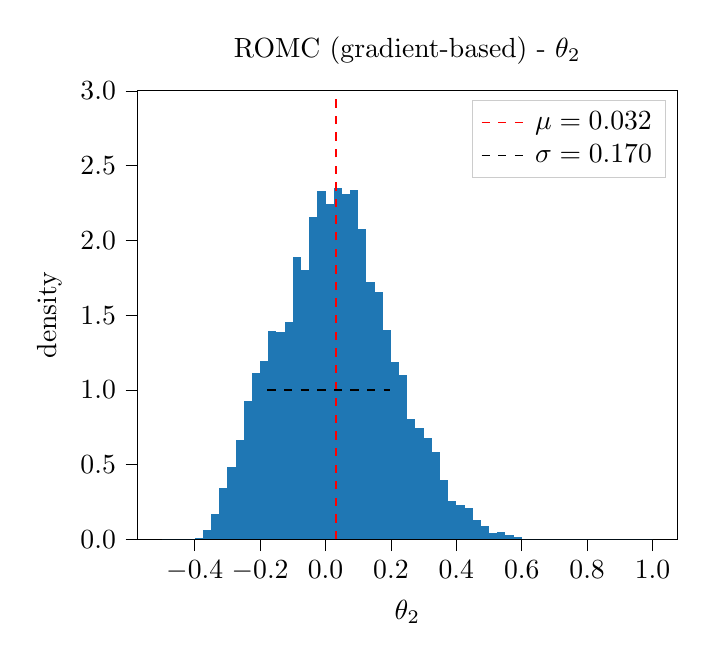
\begin{tikzpicture}

\definecolor{color0}{rgb}{0.12156862745098,0.466666666666667,0.705882352941177}

\begin{axis}[
legend cell align={left},
legend style={fill opacity=0.8, draw opacity=1, text opacity=1, draw=white!80!black},
tick align=outside,
tick pos=left,
title={ROMC (gradient-based) - \(\displaystyle \theta_2\)},
x grid style={white!69.0196078431373!black},
xlabel={\(\displaystyle \theta_2\)},
xmin=-0.575, xmax=1.075,
xtick style={color=black},
xtick={-0.6,-0.4,-0.2,0,0.2,0.4,0.6,0.8,1,1.2},
xticklabels={
  \(\displaystyle {\ensuremath{-}0.6}\),
  \(\displaystyle {\ensuremath{-}0.4}\),
  \(\displaystyle {\ensuremath{-}0.2}\),
  \(\displaystyle {0.0}\),
  \(\displaystyle {0.2}\),
  \(\displaystyle {0.4}\),
  \(\displaystyle {0.6}\),
  \(\displaystyle {0.8}\),
  \(\displaystyle {1.0}\),
  \(\displaystyle {1.2}\)
},
y grid style={white!69.0196078431373!black},
ylabel={density},
ymin=0, ymax=3,
ytick style={color=black},
ytick={0,0.5,1,1.5,2,2.5,3},
yticklabels={
  \(\displaystyle {0.0}\),
  \(\displaystyle {0.5}\),
  \(\displaystyle {1.0}\),
  \(\displaystyle {1.5}\),
  \(\displaystyle {2.0}\),
  \(\displaystyle {2.5}\),
  \(\displaystyle {3.0}\)
}
]
\draw[draw=none,fill=color0] (axis cs:-0.5,0) rectangle (axis cs:-0.475,0);
\draw[draw=none,fill=color0] (axis cs:-0.475,0) rectangle (axis cs:-0.45,0);
\draw[draw=none,fill=color0] (axis cs:-0.45,0) rectangle (axis cs:-0.425,0);
\draw[draw=none,fill=color0] (axis cs:-0.425,0) rectangle (axis cs:-0.4,0);
\draw[draw=none,fill=color0] (axis cs:-0.4,0) rectangle (axis cs:-0.375,0.00551481774368941);
\draw[draw=none,fill=color0] (axis cs:-0.375,0) rectangle (axis cs:-0.35,0.0605814218347914);
\draw[draw=none,fill=color0] (axis cs:-0.35,0) rectangle (axis cs:-0.325,0.168699423699822);
\draw[draw=none,fill=color0] (axis cs:-0.325,0) rectangle (axis cs:-0.3,0.340262186728983);
\draw[draw=none,fill=color0] (axis cs:-0.3,0) rectangle (axis cs:-0.275,0.48172967019454);
\draw[draw=none,fill=color0] (axis cs:-0.275,0) rectangle (axis cs:-0.25,0.661723210849365);
\draw[draw=none,fill=color0] (axis cs:-0.25,0) rectangle (axis cs:-0.225,0.926167683238105);
\draw[draw=none,fill=color0] (axis cs:-0.225,0) rectangle (axis cs:-0.2,1.1131441320768);
\draw[draw=none,fill=color0] (axis cs:-0.2,0) rectangle (axis cs:-0.175,1.19038558853121);
\draw[draw=none,fill=color0] (axis cs:-0.175,0) rectangle (axis cs:-0.15,1.39560413532974);
\draw[draw=none,fill=color0] (axis cs:-0.15,0) rectangle (axis cs:-0.125,1.38890799766854);
\draw[draw=none,fill=color0] (axis cs:-0.125,0) rectangle (axis cs:-0.1,1.45486223069012);
\draw[draw=none,fill=color0] (axis cs:-0.1,0) rectangle (axis cs:-0.075,1.89014334843844);
\draw[draw=none,fill=color0] (axis cs:-0.075,0) rectangle (axis cs:-0.05,1.80399178478282);
\draw[draw=none,fill=color0] (axis cs:-0.05,0) rectangle (axis cs:-0.025,2.15561058973456);
\draw[draw=none,fill=color0] (axis cs:-0.025,0) rectangle (axis cs:0,2.33061276076321);
\draw[draw=none,fill=color0] (axis cs:0,0) rectangle (axis cs:0.025,2.24024442959031);
\draw[draw=none,fill=color0] (axis cs:0.025,0) rectangle (axis cs:0.05,2.34890403251458);
\draw[draw=none,fill=color0] (axis cs:0.05,0) rectangle (axis cs:0.0750000000000001,2.31095726097247);
\draw[draw=none,fill=color0] (axis cs:0.0750000000000001,0) rectangle (axis cs:0.1,2.33900171768764);
\draw[draw=none,fill=color0] (axis cs:0.1,0) rectangle (axis cs:0.125,2.07598627244674);
\draw[draw=none,fill=color0] (axis cs:0.125,0) rectangle (axis cs:0.15,1.71987564844275);
\draw[draw=none,fill=color0] (axis cs:0.15,0) rectangle (axis cs:0.175,1.65165022964706);
\draw[draw=none,fill=color0] (axis cs:0.175,0) rectangle (axis cs:0.2,1.40256222683377);
\draw[draw=none,fill=color0] (axis cs:0.2,0) rectangle (axis cs:0.225,1.18758980571923);
\draw[draw=none,fill=color0] (axis cs:0.225,0) rectangle (axis cs:0.25,1.0980208933351);
\draw[draw=none,fill=color0] (axis cs:0.25,0) rectangle (axis cs:0.275,0.803715750920935);
\draw[draw=none,fill=color0] (axis cs:0.275,0) rectangle (axis cs:0.3,0.742179116696122);
\draw[draw=none,fill=color0] (axis cs:0.3,0) rectangle (axis cs:0.325,0.678702875114039);
\draw[draw=none,fill=color0] (axis cs:0.325,0) rectangle (axis cs:0.35,0.583516431505742);
\draw[draw=none,fill=color0] (axis cs:0.35,0) rectangle (axis cs:0.375,0.398341719580722);
\draw[draw=none,fill=color0] (axis cs:0.375,0) rectangle (axis cs:0.4,0.257727424376927);
\draw[draw=none,fill=color0] (axis cs:0.4,0) rectangle (axis cs:0.425,0.229546935490747);
\draw[draw=none,fill=color0] (axis cs:0.425,0) rectangle (axis cs:0.45,0.210112717761985);
\draw[draw=none,fill=color0] (axis cs:0.45,0) rectangle (axis cs:0.475,0.129179090828181);
\draw[draw=none,fill=color0] (axis cs:0.475,0) rectangle (axis cs:0.5,0.0899034779939157);
\draw[draw=none,fill=color0] (axis cs:0.5,0) rectangle (axis cs:0.525,0.0431810229330879);
\draw[draw=none,fill=color0] (axis cs:0.525,0) rectangle (axis cs:0.55,0.0479789143700981);
\draw[draw=none,fill=color0] (axis cs:0.55,0) rectangle (axis cs:0.575,0.0287873486220588);
\draw[draw=none,fill=color0] (axis cs:0.575,0) rectangle (axis cs:0.6,0.0143936743110293);
\draw[draw=none,fill=color0] (axis cs:0.6,0) rectangle (axis cs:0.625,0);
\draw[draw=none,fill=color0] (axis cs:0.625,0) rectangle (axis cs:0.65,0);
\draw[draw=none,fill=color0] (axis cs:0.65,0) rectangle (axis cs:0.675,0);
\draw[draw=none,fill=color0] (axis cs:0.675,0) rectangle (axis cs:0.7,0);
\draw[draw=none,fill=color0] (axis cs:0.7,0) rectangle (axis cs:0.725,0);
\draw[draw=none,fill=color0] (axis cs:0.725,0) rectangle (axis cs:0.75,0);
\draw[draw=none,fill=color0] (axis cs:0.75,0) rectangle (axis cs:0.775,0);
\draw[draw=none,fill=color0] (axis cs:0.775,0) rectangle (axis cs:0.8,0);
\draw[draw=none,fill=color0] (axis cs:0.8,0) rectangle (axis cs:0.825,0);
\draw[draw=none,fill=color0] (axis cs:0.825,0) rectangle (axis cs:0.85,0);
\draw[draw=none,fill=color0] (axis cs:0.85,0) rectangle (axis cs:0.875,0);
\draw[draw=none,fill=color0] (axis cs:0.875,0) rectangle (axis cs:0.9,0);
\draw[draw=none,fill=color0] (axis cs:0.9,0) rectangle (axis cs:0.925,0);
\draw[draw=none,fill=color0] (axis cs:0.925,0) rectangle (axis cs:0.95,0);
\draw[draw=none,fill=color0] (axis cs:0.95,0) rectangle (axis cs:0.975,0);
\draw[draw=none,fill=color0] (axis cs:0.975,0) rectangle (axis cs:1,0);
\addplot [semithick, red, dashed]
table {%
0.0318388478807404 0
0.0318388478807404 3
};
\addlegendentry{$\mu = 0.032$}
\addplot [semithick, black, dashed]
table {%
-0.177435597378694 1
0.197481062716323 1
};
\addlegendentry{$\sigma = 0.170$}
\end{axis}

\end{tikzpicture}

    }
    \resizebox{.24\columnwidth}{!}{%
      % This file was created by tikzplotlib v0.9.9.
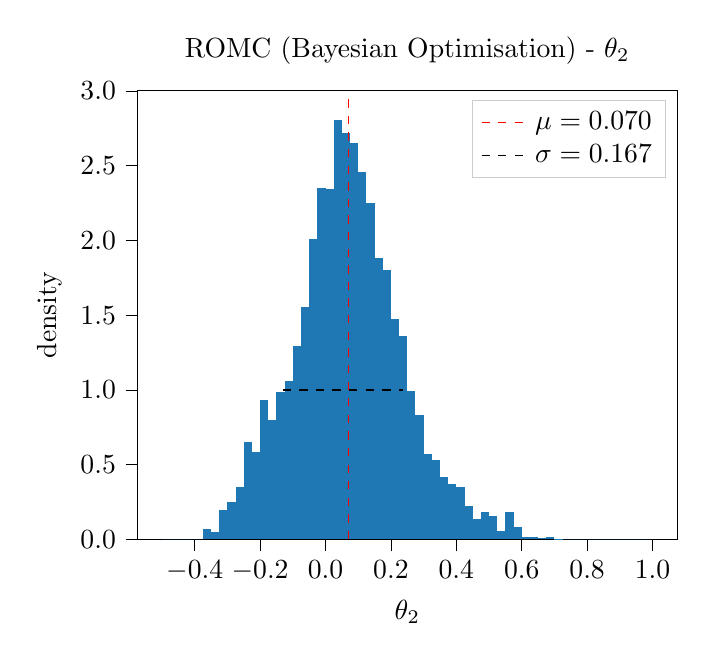
\begin{tikzpicture}

\definecolor{color0}{rgb}{0.12156862745098,0.466666666666667,0.705882352941177}

\begin{axis}[
legend cell align={left},
legend style={fill opacity=0.8, draw opacity=1, text opacity=1, draw=white!80!black},
tick align=outside,
tick pos=left,
title={ROMC (Bayesian Optimisation) - \(\displaystyle \theta_2\)},
x grid style={white!69.0196078431373!black},
xlabel={\(\displaystyle \theta_2\)},
xmin=-0.575, xmax=1.075,
xtick style={color=black},
xtick={-0.6,-0.4,-0.2,0,0.2,0.4,0.6,0.8,1,1.2},
xticklabels={
  \(\displaystyle {\ensuremath{-}0.6}\),
  \(\displaystyle {\ensuremath{-}0.4}\),
  \(\displaystyle {\ensuremath{-}0.2}\),
  \(\displaystyle {0.0}\),
  \(\displaystyle {0.2}\),
  \(\displaystyle {0.4}\),
  \(\displaystyle {0.6}\),
  \(\displaystyle {0.8}\),
  \(\displaystyle {1.0}\),
  \(\displaystyle {1.2}\)
},
y grid style={white!69.0196078431373!black},
ylabel={density},
ymin=0, ymax=3,
ytick style={color=black},
ytick={0,0.5,1,1.5,2,2.5,3},
yticklabels={
  \(\displaystyle {0.0}\),
  \(\displaystyle {0.5}\),
  \(\displaystyle {1.0}\),
  \(\displaystyle {1.5}\),
  \(\displaystyle {2.0}\),
  \(\displaystyle {2.5}\),
  \(\displaystyle {3.0}\)
}
]
\draw[draw=none,fill=color0] (axis cs:-0.5,0) rectangle (axis cs:-0.475,0);
\draw[draw=none,fill=color0] (axis cs:-0.475,0) rectangle (axis cs:-0.45,0);
\draw[draw=none,fill=color0] (axis cs:-0.45,0) rectangle (axis cs:-0.425,0);
\draw[draw=none,fill=color0] (axis cs:-0.425,0) rectangle (axis cs:-0.4,0);
\draw[draw=none,fill=color0] (axis cs:-0.4,0) rectangle (axis cs:-0.375,0);
\draw[draw=none,fill=color0] (axis cs:-0.375,0) rectangle (axis cs:-0.35,0.0710656818158832);
\draw[draw=none,fill=color0] (axis cs:-0.35,0) rectangle (axis cs:-0.325,0.0516473550957937);
\draw[draw=none,fill=color0] (axis cs:-0.325,0) rectangle (axis cs:-0.3,0.194048417709784);
\draw[draw=none,fill=color0] (axis cs:-0.3,0) rectangle (axis cs:-0.275,0.2505503544856);
\draw[draw=none,fill=color0] (axis cs:-0.275,0) rectangle (axis cs:-0.25,0.348585934523831);
\draw[draw=none,fill=color0] (axis cs:-0.25,0) rectangle (axis cs:-0.225,0.648086654282988);
\draw[draw=none,fill=color0] (axis cs:-0.225,0) rectangle (axis cs:-0.2,0.583763447022691);
\draw[draw=none,fill=color0] (axis cs:-0.2,0) rectangle (axis cs:-0.175,0.929922090706508);
\draw[draw=none,fill=color0] (axis cs:-0.175,0) rectangle (axis cs:-0.15,0.79776958941701);
\draw[draw=none,fill=color0] (axis cs:-0.15,0) rectangle (axis cs:-0.125,0.987907371884556);
\draw[draw=none,fill=color0] (axis cs:-0.125,0) rectangle (axis cs:-0.1,1.05978215064711);
\draw[draw=none,fill=color0] (axis cs:-0.1,0) rectangle (axis cs:-0.075,1.2930717702704);
\draw[draw=none,fill=color0] (axis cs:-0.075,0) rectangle (axis cs:-0.05,1.55481463251829);
\draw[draw=none,fill=color0] (axis cs:-0.05,0) rectangle (axis cs:-0.025,2.01101046094927);
\draw[draw=none,fill=color0] (axis cs:-0.025,0) rectangle (axis cs:0,2.35069632905971);
\draw[draw=none,fill=color0] (axis cs:0,0) rectangle (axis cs:0.025,2.34206596162857);
\draw[draw=none,fill=color0] (axis cs:0.025,0) rectangle (axis cs:0.05,2.80716185647295);
\draw[draw=none,fill=color0] (axis cs:0.05,0) rectangle (axis cs:0.0750000000000001,2.71681269742808);
\draw[draw=none,fill=color0] (axis cs:0.0750000000000001,0) rectangle (axis cs:0.1,2.65275918915001);
\draw[draw=none,fill=color0] (axis cs:0.1,0) rectangle (axis cs:0.125,2.45763197551135);
\draw[draw=none,fill=color0] (axis cs:0.125,0) rectangle (axis cs:0.15,2.24848041479702);
\draw[draw=none,fill=color0] (axis cs:0.15,0) rectangle (axis cs:0.175,1.8837125413398);
\draw[draw=none,fill=color0] (axis cs:0.175,0) rectangle (axis cs:0.2,1.80455589005721);
\draw[draw=none,fill=color0] (axis cs:0.2,0) rectangle (axis cs:0.225,1.47147764701123);
\draw[draw=none,fill=color0] (axis cs:0.225,0) rectangle (axis cs:0.25,1.35887832193294);
\draw[draw=none,fill=color0] (axis cs:0.25,0) rectangle (axis cs:0.275,0.990739211197902);
\draw[draw=none,fill=color0] (axis cs:0.275,0) rectangle (axis cs:0.3,0.834853199472739);
\draw[draw=none,fill=color0] (axis cs:0.3,0) rectangle (axis cs:0.325,0.568255755544842);
\draw[draw=none,fill=color0] (axis cs:0.325,0) rectangle (axis cs:0.35,0.531441844471339);
\draw[draw=none,fill=color0] (axis cs:0.35,0) rectangle (axis cs:0.375,0.415606131606362);
\draw[draw=none,fill=color0] (axis cs:0.375,0) rectangle (axis cs:0.4,0.366790615823915);
\draw[draw=none,fill=color0] (axis cs:0.4,0) rectangle (axis cs:0.425,0.350473827399395);
\draw[draw=none,fill=color0] (axis cs:0.425,0) rectangle (axis cs:0.45,0.220883466441019);
\draw[draw=none,fill=color0] (axis cs:0.45,0) rectangle (axis cs:0.475,0.136737383987297);
\draw[draw=none,fill=color0] (axis cs:0.475,0) rectangle (axis cs:0.5,0.185283200787522);
\draw[draw=none,fill=color0] (axis cs:0.5,0) rectangle (axis cs:0.525,0.154672366305157);
\draw[draw=none,fill=color0] (axis cs:0.525,0) rectangle (axis cs:0.55,0.0558276893202577);
\draw[draw=none,fill=color0] (axis cs:0.55,0) rectangle (axis cs:0.575,0.179619522160829);
\draw[draw=none,fill=color0] (axis cs:0.575,0) rectangle (axis cs:0.6,0.0788869523003634);
\draw[draw=none,fill=color0] (axis cs:0.6,0) rectangle (axis cs:0.625,0.0133500996200616);
\draw[draw=none,fill=color0] (axis cs:0.625,0) rectangle (axis cs:0.65,0.0134849491111732);
\draw[draw=none,fill=color0] (axis cs:0.65,0) rectangle (axis cs:0.675,0.00943946437782135);
\draw[draw=none,fill=color0] (axis cs:0.675,0) rectangle (axis cs:0.7,0.0140243470756202);
\draw[draw=none,fill=color0] (axis cs:0.7,0) rectangle (axis cs:0.725,0.00337123727779334);
\draw[draw=none,fill=color0] (axis cs:0.725,0) rectangle (axis cs:0.75,0);
\draw[draw=none,fill=color0] (axis cs:0.75,0) rectangle (axis cs:0.775,0);
\draw[draw=none,fill=color0] (axis cs:0.775,0) rectangle (axis cs:0.8,0);
\draw[draw=none,fill=color0] (axis cs:0.8,0) rectangle (axis cs:0.825,0);
\draw[draw=none,fill=color0] (axis cs:0.825,0) rectangle (axis cs:0.85,0);
\draw[draw=none,fill=color0] (axis cs:0.85,0) rectangle (axis cs:0.875,0);
\draw[draw=none,fill=color0] (axis cs:0.875,0) rectangle (axis cs:0.9,0);
\draw[draw=none,fill=color0] (axis cs:0.9,0) rectangle (axis cs:0.925,0);
\draw[draw=none,fill=color0] (axis cs:0.925,0) rectangle (axis cs:0.95,0);
\draw[draw=none,fill=color0] (axis cs:0.95,0) rectangle (axis cs:0.975,0);
\draw[draw=none,fill=color0] (axis cs:0.975,0) rectangle (axis cs:1,0);
\addplot [semithick, red, dashed]
table {%
0.070389896781954 0
0.070389896781954 3
};
\addlegendentry{$\mu = 0.070$}
\addplot [semithick, black, dashed]
table {%
-0.131187651225067 1
0.236045424145365 1
};
\addlegendentry{$\sigma = 0.167$}
\end{axis}

\end{tikzpicture}

    }
    \resizebox{.24\columnwidth}{!}{%
      % This file was created with tikzplotlib v0.9.12.
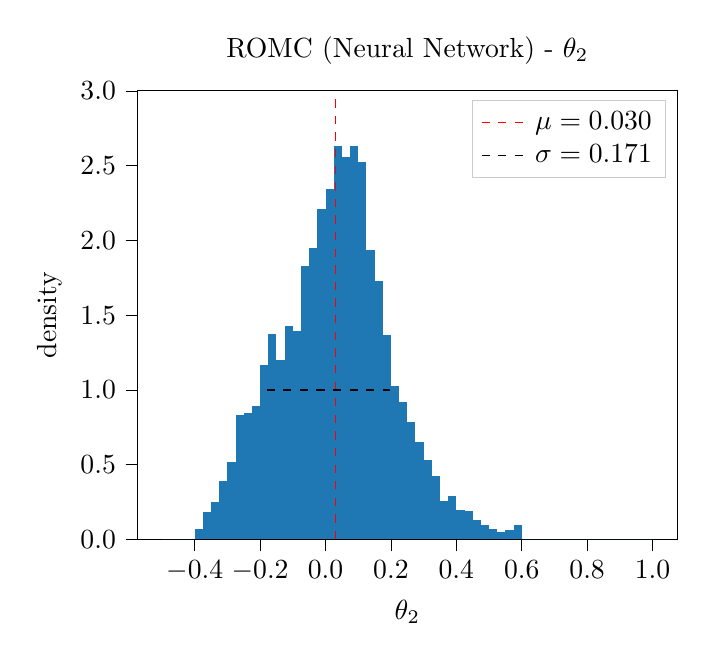
\begin{tikzpicture}

\definecolor{color0}{rgb}{0.12156862745098,0.466666666666667,0.705882352941177}

\begin{axis}[
legend cell align={left},
legend style={fill opacity=0.8, draw opacity=1, text opacity=1, draw=white!80!black},
tick align=outside,
tick pos=left,
title={ROMC (Neural Network) - \(\displaystyle \theta_2\)},
x grid style={white!69.0196078431373!black},
xlabel={\(\displaystyle \theta_2\)},
xmin=-0.575, xmax=1.075,
xtick style={color=black},
xtick={-0.6,-0.4,-0.2,0,0.2,0.4,0.6,0.8,1,1.2},
xticklabels={
  \(\displaystyle {\ensuremath{-}0.6}\),
  \(\displaystyle {\ensuremath{-}0.4}\),
  \(\displaystyle {\ensuremath{-}0.2}\),
  \(\displaystyle {0.0}\),
  \(\displaystyle {0.2}\),
  \(\displaystyle {0.4}\),
  \(\displaystyle {0.6}\),
  \(\displaystyle {0.8}\),
  \(\displaystyle {1.0}\),
  \(\displaystyle {1.2}\)
},
y grid style={white!69.0196078431373!black},
ylabel={density},
ymin=0, ymax=3,
ytick style={color=black},
ytick={0,0.5,1,1.5,2,2.5,3},
yticklabels={
  \(\displaystyle {0.0}\),
  \(\displaystyle {0.5}\),
  \(\displaystyle {1.0}\),
  \(\displaystyle {1.5}\),
  \(\displaystyle {2.0}\),
  \(\displaystyle {2.5}\),
  \(\displaystyle {3.0}\)
}
]
\draw[draw=none,fill=color0] (axis cs:-0.5,0) rectangle (axis cs:-0.475,0);
\draw[draw=none,fill=color0] (axis cs:-0.475,0) rectangle (axis cs:-0.45,0);
\draw[draw=none,fill=color0] (axis cs:-0.45,0) rectangle (axis cs:-0.425,0);
\draw[draw=none,fill=color0] (axis cs:-0.425,0) rectangle (axis cs:-0.4,0);
\draw[draw=none,fill=color0] (axis cs:-0.4,0) rectangle (axis cs:-0.375,0.0687105672242381);
\draw[draw=none,fill=color0] (axis cs:-0.375,0) rectangle (axis cs:-0.35,0.184372208227465);
\draw[draw=none,fill=color0] (axis cs:-0.35,0) rectangle (axis cs:-0.325,0.251601377874948);
\draw[draw=none,fill=color0] (axis cs:-0.325,0) rectangle (axis cs:-0.3,0.39271865402813);
\draw[draw=none,fill=color0] (axis cs:-0.3,0) rectangle (axis cs:-0.275,0.516086691042045);
\draw[draw=none,fill=color0] (axis cs:-0.275,0) rectangle (axis cs:-0.25,0.829805712987072);
\draw[draw=none,fill=color0] (axis cs:-0.25,0) rectangle (axis cs:-0.225,0.847041859829425);
\draw[draw=none,fill=color0] (axis cs:-0.225,0) rectangle (axis cs:-0.2,0.888673668222991);
\draw[draw=none,fill=color0] (axis cs:-0.2,0) rectangle (axis cs:-0.175,1.16327691119626);
\draw[draw=none,fill=color0] (axis cs:-0.175,0) rectangle (axis cs:-0.15,1.37486835291373);
\draw[draw=none,fill=color0] (axis cs:-0.15,0) rectangle (axis cs:-0.125,1.19991232691807);
\draw[draw=none,fill=color0] (axis cs:-0.125,0) rectangle (axis cs:-0.1,1.42636185782617);
\draw[draw=none,fill=color0] (axis cs:-0.1,0) rectangle (axis cs:-0.075,1.39151225358654);
\draw[draw=none,fill=color0] (axis cs:-0.075,0) rectangle (axis cs:-0.05,1.82926351678107);
\draw[draw=none,fill=color0] (axis cs:-0.05,0) rectangle (axis cs:-0.025,1.94594508515498);
\draw[draw=none,fill=color0] (axis cs:-0.025,0) rectangle (axis cs:0,2.2129470534662);
\draw[draw=none,fill=color0] (axis cs:0,0) rectangle (axis cs:0.025,2.34655785188779);
\draw[draw=none,fill=color0] (axis cs:0.025,0) rectangle (axis cs:0.05,2.63158719290653);
\draw[draw=none,fill=color0] (axis cs:0.05,0) rectangle (axis cs:0.0750000000000001,2.55685248411093);
\draw[draw=none,fill=color0] (axis cs:0.0750000000000001,0) rectangle (axis cs:0.1,2.63080691718184);
\draw[draw=none,fill=color0] (axis cs:0.1,0) rectangle (axis cs:0.125,2.52614922878044);
\draw[draw=none,fill=color0] (axis cs:0.125,0) rectangle (axis cs:0.15,1.93355077757299);
\draw[draw=none,fill=color0] (axis cs:0.15,0) rectangle (axis cs:0.175,1.72788273613444);
\draw[draw=none,fill=color0] (axis cs:0.175,0) rectangle (axis cs:0.2,1.36820910319437);
\draw[draw=none,fill=color0] (axis cs:0.2,0) rectangle (axis cs:0.225,1.0258751741395);
\draw[draw=none,fill=color0] (axis cs:0.225,0) rectangle (axis cs:0.25,0.915348210439271);
\draw[draw=none,fill=color0] (axis cs:0.25,0) rectangle (axis cs:0.275,0.784575688430834);
\draw[draw=none,fill=color0] (axis cs:0.275,0) rectangle (axis cs:0.3,0.649930571025344);
\draw[draw=none,fill=color0] (axis cs:0.3,0) rectangle (axis cs:0.325,0.528011081166735);
\draw[draw=none,fill=color0] (axis cs:0.325,0) rectangle (axis cs:0.35,0.423788895495386);
\draw[draw=none,fill=color0] (axis cs:0.35,0) rectangle (axis cs:0.375,0.255909163140911);
\draw[draw=none,fill=color0] (axis cs:0.375,0) rectangle (axis cs:0.4,0.28970067094874);
\draw[draw=none,fill=color0] (axis cs:0.4,0) rectangle (axis cs:0.425,0.19412252617457);
\draw[draw=none,fill=color0] (axis cs:0.425,0) rectangle (axis cs:0.45,0.189105171805318);
\draw[draw=none,fill=color0] (axis cs:0.45,0) rectangle (axis cs:0.475,0.127165545733375);
\draw[draw=none,fill=color0] (axis cs:0.475,0) rectangle (axis cs:0.5,0.0974061925124961);
\draw[draw=none,fill=color0] (axis cs:0.5,0) rectangle (axis cs:0.525,0.0718579504601718);
\draw[draw=none,fill=color0] (axis cs:0.525,0) rectangle (axis cs:0.55,0.0457277866564734);
\draw[draw=none,fill=color0] (axis cs:0.55,0) rectangle (axis cs:0.575,0.0587928685583229);
\draw[draw=none,fill=color0] (axis cs:0.575,0) rectangle (axis cs:0.6,0.0979881142638707);
\draw[draw=none,fill=color0] (axis cs:0.6,0) rectangle (axis cs:0.625,0);
\draw[draw=none,fill=color0] (axis cs:0.625,0) rectangle (axis cs:0.65,0);
\draw[draw=none,fill=color0] (axis cs:0.65,0) rectangle (axis cs:0.675,0);
\draw[draw=none,fill=color0] (axis cs:0.675,0) rectangle (axis cs:0.7,0);
\draw[draw=none,fill=color0] (axis cs:0.7,0) rectangle (axis cs:0.725,0);
\draw[draw=none,fill=color0] (axis cs:0.725,0) rectangle (axis cs:0.75,0);
\draw[draw=none,fill=color0] (axis cs:0.75,0) rectangle (axis cs:0.775,0);
\draw[draw=none,fill=color0] (axis cs:0.775,0) rectangle (axis cs:0.8,0);
\draw[draw=none,fill=color0] (axis cs:0.8,0) rectangle (axis cs:0.825,0);
\draw[draw=none,fill=color0] (axis cs:0.825,0) rectangle (axis cs:0.85,0);
\draw[draw=none,fill=color0] (axis cs:0.85,0) rectangle (axis cs:0.875,0);
\draw[draw=none,fill=color0] (axis cs:0.875,0) rectangle (axis cs:0.9,0);
\draw[draw=none,fill=color0] (axis cs:0.9,0) rectangle (axis cs:0.925,0);
\draw[draw=none,fill=color0] (axis cs:0.925,0) rectangle (axis cs:0.95,0);
\draw[draw=none,fill=color0] (axis cs:0.95,0) rectangle (axis cs:0.975,0);
\draw[draw=none,fill=color0] (axis cs:0.975,0) rectangle (axis cs:1,0);
\addplot [semithick, red, dashed]
table {%
0.0301562808023854 0
0.0301562808023854 3
};
\addlegendentry{$\mu = 0.030$}
\addplot [semithick, black, dashed]
table {%
-0.180267449762181 1
0.196611267527429 1
};
\addlegendentry{$\sigma = 0.171$}
\end{axis}

\end{tikzpicture}

    }
    \end{center}
    \caption[MA2 example, evaluation of the marginal
    distributions.]{Histogram of the marginal posterior distributions
      using three different inference approaches; (a) in the first
      row, the samples are obtained using Rejection ABC sampling (b)
      in the second row, using ROMC with a gradient-based optimiser
      and (c) in the third row, using ROMC with Bayesian optimisation
      approach. The vertical (red) line represents the samples mean
      \(\mu\) and the horizontal (black) the standard deviation
      \(\sigma\).}
  \label{fig:ma2_3}
\end{figure}

\begin{figure}[ht]
  \begin{center}
    \resizebox{.32\columnwidth}{!}{%
      % This file was created with tikzplotlib v0.9.12.
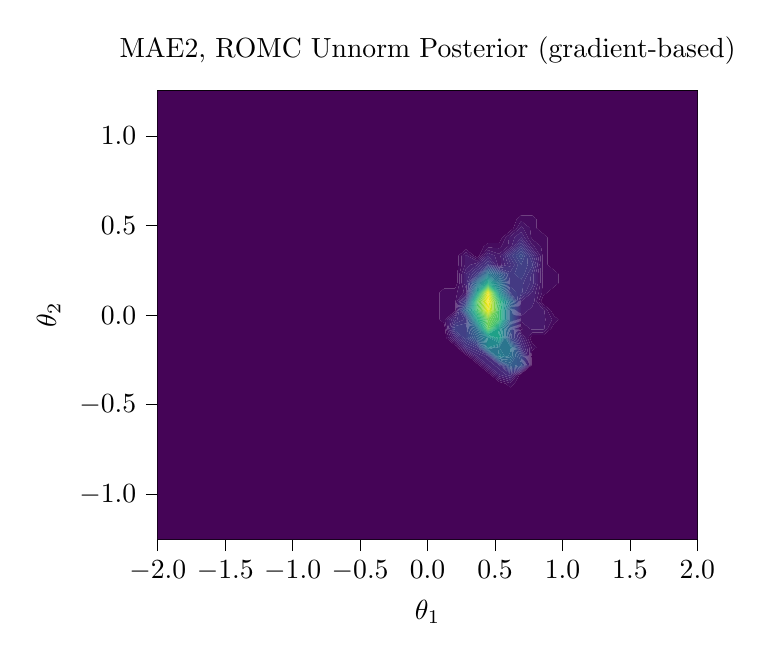
\begin{tikzpicture}

\definecolor{color0}{rgb}{0.269944,0.014625,0.341379}
\definecolor{color1}{rgb}{0.276022,0.044167,0.370164}
\definecolor{color2}{rgb}{0.280267,0.073417,0.397163}
\definecolor{color3}{rgb}{0.282656,0.100196,0.42216}
\definecolor{color4}{rgb}{0.283072,0.130895,0.449241}
\definecolor{color5}{rgb}{0.281412,0.155834,0.469201}
\definecolor{color6}{rgb}{0.278012,0.180367,0.486697}
\definecolor{color7}{rgb}{0.273006,0.20452,0.501721}
\definecolor{color8}{rgb}{0.26658,0.228262,0.514349}
\definecolor{color9}{rgb}{0.258965,0.251537,0.524736}
\definecolor{color10}{rgb}{0.250425,0.27429,0.533103}
\definecolor{color11}{rgb}{0.241237,0.296485,0.539709}
\definecolor{color12}{rgb}{0.229739,0.322361,0.545706}
\definecolor{color13}{rgb}{0.220057,0.343307,0.549413}
\definecolor{color14}{rgb}{0.210503,0.363727,0.552206}
\definecolor{color15}{rgb}{0.201239,0.38367,0.554294}
\definecolor{color16}{rgb}{0.192357,0.403199,0.555836}
\definecolor{color17}{rgb}{0.183898,0.422383,0.556944}
\definecolor{color18}{rgb}{0.175841,0.44129,0.557685}
\definecolor{color19}{rgb}{0.168126,0.459988,0.558082}
\definecolor{color20}{rgb}{0.160665,0.47854,0.558115}
\definecolor{color21}{rgb}{0.151918,0.500685,0.557587}
\definecolor{color22}{rgb}{0.144759,0.519093,0.556572}
\definecolor{color23}{rgb}{0.13777,0.537492,0.554906}
\definecolor{color24}{rgb}{0.131172,0.555899,0.552459}
\definecolor{color25}{rgb}{0.125394,0.574318,0.549086}
\definecolor{color26}{rgb}{0.121148,0.592739,0.544641}
\definecolor{color27}{rgb}{0.119423,0.611141,0.538982}
\definecolor{color28}{rgb}{0.12138,0.629492,0.531973}
\definecolor{color29}{rgb}{0.130067,0.651384,0.521608}
\definecolor{color30}{rgb}{0.143303,0.669459,0.511215}
\definecolor{color31}{rgb}{0.162016,0.687316,0.499129}
\definecolor{color32}{rgb}{0.185783,0.704891,0.485273}
\definecolor{color33}{rgb}{0.214,0.722114,0.469588}
\definecolor{color34}{rgb}{0.24607,0.73891,0.452024}
\definecolor{color35}{rgb}{0.281477,0.755203,0.432552}
\definecolor{color36}{rgb}{0.319809,0.770914,0.411152}
\definecolor{color37}{rgb}{0.369214,0.788888,0.382914}
\definecolor{color38}{rgb}{0.412913,0.803041,0.357269}
\definecolor{color39}{rgb}{0.458674,0.816363,0.329727}
\definecolor{color40}{rgb}{0.506271,0.828786,0.300362}
\definecolor{color41}{rgb}{0.555484,0.840254,0.269281}
\definecolor{color42}{rgb}{0.606045,0.850733,0.236712}
\definecolor{color43}{rgb}{0.657642,0.860219,0.203082}
\definecolor{color44}{rgb}{0.709898,0.868751,0.169257}
\definecolor{color45}{rgb}{0.762373,0.876424,0.137064}
\definecolor{color46}{rgb}{0.82494,0.88472,0.106217}
\definecolor{color47}{rgb}{0.876168,0.891125,0.09525}
\definecolor{color48}{rgb}{0.926106,0.89733,0.104071}
\definecolor{color49}{rgb}{0.974417,0.90359,0.130215}

\begin{axis}[
tick align=outside,
tick pos=left,
title={MAE2, ROMC Unnorm Posterior (gradient-based)},
x grid style={white!69.0196078431373!black},
xlabel={\(\displaystyle \theta_1\)},
xmin=-2, xmax=2,
xtick style={color=black},
xtick={-2,-1.5,-1,-0.5,0,0.5,1,1.5,2},
xticklabels={
  \(\displaystyle {\ensuremath{-}2.0}\),
  \(\displaystyle {\ensuremath{-}1.5}\),
  \(\displaystyle {\ensuremath{-}1.0}\),
  \(\displaystyle {\ensuremath{-}0.5}\),
  \(\displaystyle {0.0}\),
  \(\displaystyle {0.5}\),
  \(\displaystyle {1.0}\),
  \(\displaystyle {1.5}\),
  \(\displaystyle {2.0}\)
},
y grid style={white!69.0196078431373!black},
ylabel={\(\displaystyle \theta_2\)},
ymin=-1.25, ymax=1.25,
ytick style={color=black},
ytick={-1.5,-1,-0.5,0,0.5,1,1.5},
yticklabels={
  \(\displaystyle {\ensuremath{-}1.5}\),
  \(\displaystyle {\ensuremath{-}1.0}\),
  \(\displaystyle {\ensuremath{-}0.5}\),
  \(\displaystyle {0.0}\),
  \(\displaystyle {0.5}\),
  \(\displaystyle {1.0}\),
  \(\displaystyle {1.5}\)
}
]
\addplot [draw=none, fill=color0]
table{%
x  y
-1.91836734693878 -1.25
-1.83673469387755 -1.25
-1.75510204081633 -1.25
-1.6734693877551 -1.25
-1.59183673469388 -1.25
-1.51020408163265 -1.25
-1.42857142857143 -1.25
-1.3469387755102 -1.25
-1.26530612244898 -1.25
-1.18367346938776 -1.25
-1.10204081632653 -1.25
-1.02040816326531 -1.25
-0.938775510204082 -1.25
-0.857142857142857 -1.25
-0.775510204081633 -1.25
-0.693877551020408 -1.25
-0.612244897959184 -1.25
-0.530612244897959 -1.25
-0.448979591836735 -1.25
-0.36734693877551 -1.25
-0.285714285714286 -1.25
-0.204081632653061 -1.25
-0.122448979591837 -1.25
-0.0408163265306123 -1.25
0.0408163265306123 -1.25
0.122448979591836 -1.25
0.204081632653061 -1.25
0.285714285714286 -1.25
0.36734693877551 -1.25
0.448979591836734 -1.25
0.530612244897959 -1.25
0.612244897959183 -1.25
0.693877551020408 -1.25
0.775510204081633 -1.25
0.857142857142857 -1.25
0.938775510204081 -1.25
1.02040816326531 -1.25
1.10204081632653 -1.25
1.18367346938775 -1.25
1.26530612244898 -1.25
1.3469387755102 -1.25
1.42857142857143 -1.25
1.51020408163265 -1.25
1.59183673469388 -1.25
1.6734693877551 -1.25
1.75510204081633 -1.25
1.83673469387755 -1.25
1.91836734693878 -1.25
2 -1.25
2 -1.19897959183673
2 -1.14795918367347
2 -1.0969387755102
2 -1.04591836734694
2 -0.994897959183674
2 -0.943877551020408
2 -0.892857142857143
2 -0.841836734693878
2 -0.790816326530612
2 -0.739795918367347
2 -0.688775510204082
2 -0.637755102040816
2 -0.586734693877551
2 -0.535714285714286
2 -0.48469387755102
2 -0.433673469387755
2 -0.38265306122449
2 -0.331632653061224
2 -0.280612244897959
2 -0.229591836734694
2 -0.178571428571429
2 -0.127551020408163
2 -0.0765306122448979
2 -0.0255102040816326
2 0.0255102040816326
2 0.0765306122448979
2 0.127551020408163
2 0.178571428571429
2 0.229591836734694
2 0.280612244897959
2 0.331632653061225
2 0.38265306122449
2 0.433673469387755
2 0.48469387755102
2 0.535714285714286
2 0.586734693877551
2 0.637755102040816
2 0.688775510204082
2 0.739795918367347
2 0.790816326530612
2 0.841836734693878
2 0.892857142857143
2 0.943877551020408
2 0.994897959183674
2 1.04591836734694
2 1.0969387755102
2 1.14795918367347
2 1.19897959183673
2 1.25
1.91836734693878 1.25
1.83673469387755 1.25
1.75510204081633 1.25
1.6734693877551 1.25
1.59183673469388 1.25
1.51020408163265 1.25
1.42857142857143 1.25
1.3469387755102 1.25
1.26530612244898 1.25
1.18367346938775 1.25
1.10204081632653 1.25
1.02040816326531 1.25
0.938775510204081 1.25
0.857142857142857 1.25
0.775510204081633 1.25
0.693877551020408 1.25
0.612244897959183 1.25
0.530612244897959 1.25
0.448979591836734 1.25
0.36734693877551 1.25
0.285714285714286 1.25
0.204081632653061 1.25
0.122448979591836 1.25
0.0408163265306123 1.25
-0.0408163265306123 1.25
-0.122448979591837 1.25
-0.204081632653061 1.25
-0.285714285714286 1.25
-0.36734693877551 1.25
-0.448979591836735 1.25
-0.530612244897959 1.25
-0.612244897959184 1.25
-0.693877551020408 1.25
-0.775510204081633 1.25
-0.857142857142857 1.25
-0.938775510204082 1.25
-1.02040816326531 1.25
-1.10204081632653 1.25
-1.18367346938776 1.25
-1.26530612244898 1.25
-1.3469387755102 1.25
-1.42857142857143 1.25
-1.51020408163265 1.25
-1.59183673469388 1.25
-1.6734693877551 1.25
-1.75510204081633 1.25
-1.83673469387755 1.25
-1.91836734693878 1.25
-2 1.25
-2 1.19897959183673
-2 1.14795918367347
-2 1.0969387755102
-2 1.04591836734694
-2 0.994897959183674
-2 0.943877551020408
-2 0.892857142857143
-2 0.841836734693878
-2 0.790816326530612
-2 0.739795918367347
-2 0.688775510204082
-2 0.637755102040816
-2 0.586734693877551
-2 0.535714285714286
-2 0.48469387755102
-2 0.433673469387755
-2 0.38265306122449
-2 0.331632653061225
-2 0.280612244897959
-2 0.229591836734694
-2 0.178571428571429
-2 0.127551020408163
-2 0.0765306122448979
-2 0.0255102040816326
-2 -0.0255102040816326
-2 -0.0765306122448979
-2 -0.127551020408163
-2 -0.178571428571429
-2 -0.229591836734694
-2 -0.280612244897959
-2 -0.331632653061224
-2 -0.38265306122449
-2 -0.433673469387755
-2 -0.48469387755102
-2 -0.535714285714286
-2 -0.586734693877551
-2 -0.637755102040816
-2 -0.688775510204082
-2 -0.739795918367347
-2 -0.790816326530612
-2 -0.841836734693878
-2 -0.892857142857143
-2 -0.943877551020408
-2 -0.994897959183674
-2 -1.04591836734694
-2 -1.0969387755102
-2 -1.14795918367347
-2 -1.19897959183673
-2 -1.25
-1.91836734693878 -1.25

0.579591836734694 -0.38265306122449
0.530612244897959 -0.372448979591837
0.465306122448979 -0.331632653061224
0.448979591836734 -0.321428571428571
0.383673469387755 -0.280612244897959
0.36734693877551 -0.270408163265306
0.302040816326531 -0.229591836734694
0.285714285714286 -0.221938775510204
0.216326530612245 -0.178571428571429
0.204081632653061 -0.168367346938776
0.138775510204081 -0.127551020408163
0.130612244897959 -0.0765306122448979
0.122448979591836 -0.0459183673469387
0.0897959183673468 -0.0255102040816326
0.0897959183673468 0.0255102040816326
0.0897959183673468 0.0765306122448979
0.0897959183673468 0.127551020408163
0.122448979591836 0.147959183673469
0.204081632653061 0.147959183673469
0.220408163265306 0.178571428571429
0.220408163265306 0.229591836734694
0.228571428571428 0.280612244897959
0.228571428571428 0.331632653061225
0.285714285714286 0.36734693877551
0.342857142857143 0.331632653061225
0.36734693877551 0.321428571428572
0.383673469387755 0.331632653061225
0.416326530612245 0.38265306122449
0.448979591836734 0.403061224489796
0.530612244897959 0.403061224489796
0.555102040816326 0.433673469387755
0.612244897959183 0.469387755102041
0.636734693877551 0.48469387755102
0.661224489795918 0.535714285714286
0.693877551020408 0.556122448979592
0.775510204081633 0.556122448979592
0.808163265306122 0.535714285714286
0.808163265306122 0.48469387755102
0.857142857142857 0.454081632653061
0.889795918367347 0.433673469387755
0.889795918367347 0.38265306122449
0.889795918367347 0.331632653061225
0.889795918367347 0.280612244897959
0.938775510204081 0.25
0.971428571428571 0.229591836734694
0.971428571428571 0.178571428571429
0.938775510204081 0.158163265306123
0.889795918367347 0.127551020408163
0.857142857142857 0.107142857142857
0.840816326530612 0.0765306122448979
0.857142857142857 0.0612244897959183
0.914285714285714 0.0255102040816326
0.938775510204081 -0.00510204081632653
0.971428571428571 -0.0255102040816326
0.938775510204081 -0.0459183673469387
0.914285714285714 -0.0765306122448979
0.857142857142857 -0.112244897959184
0.775510204081633 -0.112244897959184
0.759183673469388 -0.127551020408163
0.775510204081633 -0.158163265306122
0.808163265306122 -0.178571428571429
0.775510204081633 -0.198979591836735
0.768513119533528 -0.229591836734694
0.769387755102041 -0.280612244897959
0.693877551020408 -0.32780612244898
0.681632653061224 -0.331632653061224
0.644897959183673 -0.38265306122449
0.612244897959183 -0.403061224489796
0.579591836734694 -0.38265306122449
};
\addplot [draw=none, fill=color1]
table{%
x  y
0.612244897959183 -0.403061224489796
0.644897959183673 -0.38265306122449
0.681632653061224 -0.331632653061224
0.693877551020408 -0.32780612244898
0.769387755102041 -0.280612244897959
0.768513119533528 -0.229591836734694
0.775510204081633 -0.198979591836735
0.808163265306122 -0.178571428571429
0.775510204081633 -0.158163265306122
0.759183673469388 -0.127551020408163
0.775510204081633 -0.112244897959184
0.857142857142857 -0.112244897959184
0.914285714285714 -0.0765306122448979
0.938775510204081 -0.0459183673469387
0.971428571428571 -0.0255102040816326
0.938775510204081 -0.00510204081632653
0.914285714285714 0.0255102040816326
0.857142857142857 0.0612244897959183
0.840816326530612 0.0765306122448979
0.857142857142857 0.107142857142857
0.889795918367347 0.127551020408163
0.938775510204081 0.158163265306123
0.971428571428571 0.178571428571429
0.971428571428571 0.229591836734694
0.938775510204081 0.25
0.889795918367347 0.280612244897959
0.889795918367347 0.331632653061225
0.889795918367347 0.38265306122449
0.889795918367347 0.433673469387755
0.857142857142857 0.454081632653061
0.808163265306122 0.48469387755102
0.808163265306122 0.535714285714286
0.775510204081633 0.556122448979592
0.693877551020408 0.556122448979592
0.661224489795918 0.535714285714286
0.636734693877551 0.48469387755102
0.612244897959183 0.469387755102041
0.555102040816326 0.433673469387755
0.530612244897959 0.403061224489796
0.448979591836734 0.403061224489796
0.416326530612245 0.38265306122449
0.383673469387755 0.331632653061225
0.36734693877551 0.321428571428572
0.342857142857143 0.331632653061225
0.285714285714286 0.36734693877551
0.228571428571428 0.331632653061225
0.228571428571428 0.280612244897959
0.220408163265306 0.229591836734694
0.220408163265306 0.178571428571429
0.204081632653061 0.147959183673469
0.122448979591836 0.147959183673469
0.0897959183673468 0.127551020408163
0.0897959183673468 0.0765306122448979
0.0897959183673468 0.0255102040816326
0.0897959183673468 -0.0255102040816326
0.122448979591836 -0.0459183673469387
0.130612244897959 -0.0765306122448979
0.138775510204081 -0.127551020408163
0.204081632653061 -0.168367346938776
0.216326530612245 -0.178571428571429
0.285714285714286 -0.221938775510204
0.302040816326531 -0.229591836734694
0.36734693877551 -0.270408163265306
0.383673469387755 -0.280612244897959
0.448979591836734 -0.321428571428571
0.465306122448979 -0.331632653061224
0.530612244897959 -0.372448979591837
0.579591836734694 -0.38265306122449
0.612244897959183 -0.403061224489796

0.481632653061224 -0.331632653061224
0.448979591836734 -0.311224489795918
0.4 -0.280612244897959
0.36734693877551 -0.260204081632653
0.318367346938775 -0.229591836734694
0.285714285714286 -0.214285714285714
0.228571428571428 -0.178571428571429
0.204081632653061 -0.158163265306122
0.155102040816326 -0.127551020408163
0.138775510204081 -0.0765306122448979
0.127891156462585 -0.0255102040816326
0.204081632653061 0.0221088435374149
0.205895691609977 0.0255102040816326
0.20734693877551 0.0765306122448979
0.220408163265306 0.127551020408163
0.236734693877551 0.178571428571429
0.236734693877551 0.229591836734694
0.253061224489796 0.280612244897959
0.253061224489796 0.331632653061225
0.285714285714286 0.352040816326531
0.318367346938775 0.331632653061225
0.36734693877551 0.311224489795918
0.4 0.331632653061225
0.448979591836734 0.377551020408163
0.530612244897959 0.372448979591837
0.546938775510204 0.38265306122449
0.579591836734694 0.433673469387755
0.612244897959183 0.454081632653061
0.661224489795918 0.48469387755102
0.693877551020408 0.525510204081633
0.759183673469388 0.48469387755102
0.76734693877551 0.433673469387755
0.775510204081633 0.423469387755102
0.840816326530612 0.38265306122449
0.851700680272108 0.331632653061225
0.853061224489795 0.280612244897959
0.851700680272108 0.229591836734694
0.851700680272108 0.178571428571429
0.848979591836734 0.127551020408163
0.824489795918367 0.0765306122448979
0.857142857142857 0.0459183673469387
0.889795918367347 0.0255102040816326
0.922448979591836 -0.0255102040816326
0.889795918367347 -0.0765306122448979
0.857142857142857 -0.096938775510204
0.775510204081633 -0.096938775510204
0.742857142857143 -0.127551020408163
0.770068027210884 -0.178571428571429
0.761516034985423 -0.229591836734694
0.763265306122449 -0.280612244897959
0.693877551020408 -0.323979591836735
0.669387755102041 -0.331632653061224
0.612244897959183 -0.379251700680272
0.530612244897959 -0.362244897959184
0.481632653061224 -0.331632653061224
};
\addplot [draw=none, fill=color1]
table{%
x  y
0.693877551020408 -0.0816326530612244
0.710204081632653 -0.0765306122448979
0.693877551020408 -0.0663265306122448
0.691545189504373 -0.0765306122448979
0.693877551020408 -0.0816326530612244
};
\addplot [draw=none, fill=color2]
table{%
x  y
0.530612244897959 -0.362244897959184
0.612244897959183 -0.379251700680272
0.669387755102041 -0.331632653061224
0.693877551020408 -0.323979591836735
0.763265306122449 -0.280612244897959
0.761516034985423 -0.229591836734694
0.770068027210884 -0.178571428571429
0.742857142857143 -0.127551020408163
0.775510204081633 -0.096938775510204
0.857142857142857 -0.096938775510204
0.889795918367347 -0.0765306122448979
0.922448979591836 -0.0255102040816326
0.889795918367347 0.0255102040816326
0.857142857142857 0.0459183673469387
0.824489795918367 0.0765306122448979
0.848979591836734 0.127551020408163
0.851700680272109 0.178571428571429
0.851700680272109 0.229591836734694
0.853061224489795 0.280612244897959
0.851700680272109 0.331632653061225
0.840816326530612 0.38265306122449
0.775510204081633 0.423469387755102
0.76734693877551 0.433673469387755
0.759183673469388 0.48469387755102
0.693877551020408 0.525510204081633
0.661224489795918 0.48469387755102
0.612244897959183 0.454081632653061
0.579591836734694 0.433673469387755
0.546938775510204 0.38265306122449
0.530612244897959 0.372448979591837
0.448979591836734 0.377551020408163
0.4 0.331632653061225
0.36734693877551 0.311224489795918
0.318367346938775 0.331632653061225
0.285714285714286 0.352040816326531
0.253061224489796 0.331632653061225
0.253061224489796 0.280612244897959
0.236734693877551 0.229591836734694
0.236734693877551 0.178571428571429
0.220408163265306 0.127551020408163
0.20734693877551 0.0765306122448979
0.205895691609977 0.0255102040816326
0.204081632653061 0.0221088435374149
0.127891156462585 -0.0255102040816326
0.138775510204081 -0.0765306122448979
0.155102040816326 -0.127551020408163
0.204081632653061 -0.158163265306122
0.228571428571428 -0.178571428571429
0.285714285714286 -0.214285714285714
0.318367346938775 -0.229591836734694
0.36734693877551 -0.260204081632653
0.4 -0.280612244897959
0.448979591836734 -0.311224489795918
0.481632653061224 -0.331632653061224
0.530612244897959 -0.362244897959184

0.497959183673469 -0.331632653061224
0.448979591836734 -0.301020408163265
0.416326530612245 -0.280612244897959
0.36734693877551 -0.25
0.33469387755102 -0.229591836734694
0.285714285714286 -0.206632653061224
0.240816326530612 -0.178571428571429
0.204081632653061 -0.147959183673469
0.171428571428571 -0.127551020408163
0.146938775510204 -0.0765306122448979
0.14421768707483 -0.0255102040816326
0.204081632653061 0.0119047619047619
0.211337868480725 0.0255102040816326
0.217142857142857 0.0765306122448979
0.269387755102041 0.127551020408163
0.253061224489796 0.178571428571429
0.253061224489796 0.229591836734694
0.277551020408163 0.280612244897959
0.277551020408163 0.331632653061225
0.285714285714286 0.336734693877551
0.293877551020408 0.331632653061225
0.36734693877551 0.301020408163265
0.416326530612245 0.331632653061225
0.448979591836734 0.362244897959184
0.530612244897959 0.341836734693878
0.595918367346939 0.38265306122449
0.604081632653061 0.433673469387755
0.612244897959183 0.438775510204082
0.685714285714285 0.48469387755102
0.693877551020408 0.494897959183673
0.710204081632653 0.48469387755102
0.742857142857143 0.433673469387755
0.775510204081633 0.392857142857143
0.791836734693877 0.38265306122449
0.835374149659864 0.331632653061225
0.840816326530612 0.280612244897959
0.835374149659864 0.229591836734694
0.835374149659864 0.178571428571429
0.824489795918367 0.127551020408163
0.808163265306122 0.0765306122448979
0.857142857142857 0.0306122448979591
0.865306122448979 0.0255102040816326
0.873469387755102 -0.0255102040816326
0.865306122448979 -0.0765306122448979
0.857142857142857 -0.0816326530612244
0.775510204081633 -0.0816326530612244
0.759183673469388 -0.0765306122448979
0.693877551020408 -0.0357142857142857
0.684548104956268 -0.0765306122448979
0.693877551020408 -0.096938775510204
0.726530612244898 -0.127551020408163
0.753741496598639 -0.178571428571429
0.754518950437318 -0.229591836734694
0.757142857142857 -0.280612244897959
0.693877551020408 -0.32015306122449
0.657142857142857 -0.331632653061224
0.612244897959183 -0.369047619047619
0.530612244897959 -0.352040816326531
0.497959183673469 -0.331632653061224

0.691545189504373 -0.0765306122448979
0.693877551020408 -0.0663265306122448
0.710204081632653 -0.0765306122448979
0.693877551020408 -0.0816326530612244
0.691545189504373 -0.0765306122448979
};
\addplot [draw=none, fill=color3]
table{%
x  y
0.530612244897959 -0.352040816326531
0.612244897959183 -0.369047619047619
0.657142857142857 -0.331632653061224
0.693877551020408 -0.32015306122449
0.757142857142857 -0.280612244897959
0.754518950437318 -0.229591836734694
0.753741496598639 -0.178571428571429
0.726530612244898 -0.127551020408163
0.693877551020408 -0.096938775510204
0.684548104956268 -0.0765306122448979
0.693877551020408 -0.0357142857142857
0.759183673469388 -0.0765306122448979
0.775510204081633 -0.0816326530612244
0.857142857142857 -0.0816326530612244
0.865306122448979 -0.0765306122448979
0.873469387755102 -0.0255102040816326
0.865306122448979 0.0255102040816326
0.857142857142857 0.0306122448979591
0.808163265306122 0.0765306122448979
0.824489795918367 0.127551020408163
0.835374149659864 0.178571428571429
0.835374149659864 0.229591836734694
0.840816326530612 0.280612244897959
0.835374149659864 0.331632653061225
0.791836734693877 0.38265306122449
0.775510204081633 0.392857142857143
0.742857142857143 0.433673469387755
0.710204081632653 0.48469387755102
0.693877551020408 0.494897959183673
0.685714285714285 0.48469387755102
0.612244897959183 0.438775510204082
0.604081632653061 0.433673469387755
0.595918367346939 0.38265306122449
0.530612244897959 0.341836734693878
0.448979591836734 0.362244897959184
0.416326530612245 0.331632653061225
0.36734693877551 0.301020408163265
0.293877551020408 0.331632653061225
0.285714285714286 0.336734693877551
0.277551020408163 0.331632653061225
0.277551020408163 0.280612244897959
0.253061224489796 0.229591836734694
0.253061224489796 0.178571428571429
0.269387755102041 0.127551020408163
0.217142857142857 0.0765306122448979
0.211337868480725 0.0255102040816326
0.204081632653061 0.0119047619047619
0.14421768707483 -0.0255102040816326
0.146938775510204 -0.0765306122448979
0.171428571428571 -0.127551020408163
0.204081632653061 -0.147959183673469
0.240816326530612 -0.178571428571429
0.285714285714286 -0.206632653061224
0.33469387755102 -0.229591836734694
0.36734693877551 -0.25
0.416326530612245 -0.280612244897959
0.448979591836734 -0.301020408163265
0.497959183673469 -0.331632653061224
0.530612244897959 -0.352040816326531

0.514285714285714 -0.331632653061224
0.448979591836734 -0.290816326530612
0.432653061224489 -0.280612244897959
0.36734693877551 -0.239795918367347
0.351020408163265 -0.229591836734694
0.285714285714286 -0.198979591836735
0.253061224489796 -0.178571428571429
0.204081632653061 -0.137755102040816
0.187755102040816 -0.127551020408163
0.155102040816326 -0.0765306122448979
0.160544217687075 -0.0255102040816326
0.204081632653061 0.00170068027210884
0.216780045351474 0.0255102040816326
0.226938775510204 0.0765306122448979
0.285714285714286 0.122448979591837
0.288046647230321 0.127551020408163
0.285714285714286 0.147959183673469
0.269387755102041 0.178571428571429
0.269387755102041 0.229591836734694
0.285714285714286 0.260204081632653
0.318367346938775 0.280612244897959
0.36734693877551 0.290816326530612
0.432653061224489 0.331632653061225
0.448979591836734 0.346938775510204
0.497959183673469 0.331632653061225
0.519727891156462 0.280612244897959
0.530612244897959 0.277696793002916
0.546938775510204 0.280612244897959
0.541496598639456 0.331632653061225
0.612244897959183 0.375850340136054
0.62312925170068 0.38265306122449
0.644897959183673 0.433673469387755
0.693877551020408 0.464285714285714
0.718367346938775 0.433673469387755
0.764625850340136 0.38265306122449
0.775510204081633 0.372448979591837
0.819047619047619 0.331632653061225
0.828571428571428 0.280612244897959
0.819047619047619 0.229591836734694
0.819047619047619 0.178571428571429
0.8 0.127551020408163
0.791836734693877 0.0765306122448979
0.775510204081633 0.0459183673469387
0.742857142857143 0.0255102040816326
0.693877551020408 -0.00510204081632651
0.689212827988338 -0.0255102040816326
0.677551020408163 -0.0765306122448979
0.693877551020408 -0.112244897959184
0.710204081632653 -0.127551020408163
0.737414965986394 -0.178571428571429
0.747521865889213 -0.229591836734694
0.751020408163265 -0.280612244897959
0.693877551020408 -0.316326530612245
0.644897959183673 -0.331632653061224
0.612244897959183 -0.358843537414966
0.530612244897959 -0.341836734693878
0.514285714285714 -0.331632653061224
};
\addplot [draw=none, fill=color4]
table{%
x  y
0.530612244897959 -0.341836734693878
0.612244897959183 -0.358843537414966
0.644897959183673 -0.331632653061224
0.693877551020408 -0.316326530612245
0.751020408163265 -0.280612244897959
0.747521865889213 -0.229591836734694
0.737414965986394 -0.178571428571429
0.710204081632653 -0.127551020408163
0.693877551020408 -0.112244897959184
0.677551020408163 -0.0765306122448979
0.689212827988338 -0.0255102040816326
0.693877551020408 -0.00510204081632651
0.742857142857143 0.0255102040816326
0.775510204081633 0.0459183673469387
0.791836734693877 0.0765306122448979
0.8 0.127551020408163
0.819047619047619 0.178571428571429
0.819047619047619 0.229591836734694
0.828571428571428 0.280612244897959
0.819047619047619 0.331632653061225
0.775510204081633 0.372448979591837
0.764625850340136 0.38265306122449
0.718367346938775 0.433673469387755
0.693877551020408 0.464285714285714
0.644897959183673 0.433673469387755
0.62312925170068 0.38265306122449
0.612244897959183 0.375850340136054
0.541496598639456 0.331632653061225
0.546938775510204 0.280612244897959
0.530612244897959 0.277696793002916
0.519727891156462 0.280612244897959
0.497959183673469 0.331632653061225
0.448979591836734 0.346938775510204
0.43265306122449 0.331632653061225
0.36734693877551 0.290816326530612
0.318367346938775 0.280612244897959
0.285714285714286 0.260204081632653
0.269387755102041 0.229591836734694
0.269387755102041 0.178571428571429
0.285714285714286 0.147959183673469
0.288046647230321 0.127551020408163
0.285714285714286 0.122448979591837
0.226938775510204 0.0765306122448979
0.216780045351474 0.0255102040816326
0.204081632653061 0.00170068027210884
0.160544217687075 -0.0255102040816326
0.155102040816326 -0.0765306122448979
0.187755102040816 -0.127551020408163
0.204081632653061 -0.137755102040816
0.253061224489796 -0.178571428571429
0.285714285714286 -0.198979591836735
0.351020408163265 -0.229591836734694
0.36734693877551 -0.239795918367347
0.43265306122449 -0.280612244897959
0.448979591836734 -0.290816326530612
0.514285714285714 -0.331632653061224
0.530612244897959 -0.341836734693878

0.530612244897959 -0.331632653061224
0.530612244897959 -0.331632653061224
0.448979591836734 -0.280612244897959
0.448979591836734 -0.280612244897959
0.36734693877551 -0.229591836734694
0.36734693877551 -0.229591836734694
0.285714285714286 -0.191326530612245
0.265306122448979 -0.178571428571429
0.204081632653061 -0.127551020408163
0.204081632653061 -0.127551020408163
0.163265306122449 -0.0765306122448979
0.17687074829932 -0.0255102040816326
0.204081632653061 -0.00850340136054422
0.222222222222222 0.0255102040816326
0.236734693877551 0.0765306122448979
0.285714285714286 0.114795918367347
0.291545189504373 0.127551020408163
0.285714285714286 0.178571428571429
0.285714285714286 0.229591836734694
0.36734693877551 0.280612244897959
0.36734693877551 0.280612244897959
0.448979591836734 0.331632653061225
0.503401360544217 0.280612244897959
0.530612244897959 0.27332361516035
0.571428571428571 0.280612244897959
0.5578231292517 0.331632653061225
0.612244897959183 0.365646258503401
0.639455782312925 0.38265306122449
0.693877551020408 0.433673469387755
0.748299319727891 0.38265306122449
0.775510204081633 0.357142857142857
0.802721088435374 0.331632653061225
0.816326530612245 0.280612244897959
0.802721088435374 0.229591836734694
0.802721088435374 0.178571428571429
0.775510204081633 0.127551020408163
0.775510204081633 0.127551020408163
0.693877551020408 0.0765306122448979
0.693877551020408 0.0765306122448979
0.693877551020408 0.0255102040816326
0.682215743440233 -0.0255102040816326
0.670553935860058 -0.0765306122448979
0.693877551020408 -0.127551020408163
0.693877551020408 -0.127551020408163
0.72108843537415 -0.178571428571429
0.740524781341108 -0.229591836734694
0.744897959183674 -0.280612244897959
0.693877551020408 -0.3125
0.63265306122449 -0.331632653061224
0.612244897959183 -0.348639455782313
0.530612244897959 -0.331632653061224
};
\addplot [draw=none, fill=color5]
table{%
x  y
0.612244897959183 -0.348639455782313
0.63265306122449 -0.331632653061224
0.693877551020408 -0.3125
0.744897959183673 -0.280612244897959
0.740524781341108 -0.229591836734694
0.72108843537415 -0.178571428571429
0.693877551020408 -0.127551020408163
0.693877551020408 -0.127551020408163
0.670553935860058 -0.0765306122448979
0.682215743440233 -0.0255102040816326
0.693877551020408 0.0255102040816326
0.693877551020408 0.0765306122448979
0.693877551020408 0.0765306122448979
0.775510204081633 0.127551020408163
0.775510204081633 0.127551020408163
0.802721088435374 0.178571428571429
0.802721088435374 0.229591836734694
0.816326530612245 0.280612244897959
0.802721088435374 0.331632653061225
0.775510204081633 0.357142857142857
0.748299319727891 0.38265306122449
0.693877551020408 0.433673469387755
0.639455782312925 0.38265306122449
0.612244897959183 0.365646258503401
0.5578231292517 0.331632653061225
0.571428571428571 0.280612244897959
0.530612244897959 0.27332361516035
0.503401360544217 0.280612244897959
0.448979591836734 0.331632653061225
0.36734693877551 0.280612244897959
0.36734693877551 0.280612244897959
0.285714285714286 0.229591836734694
0.285714285714286 0.178571428571429
0.291545189504373 0.127551020408163
0.285714285714286 0.114795918367347
0.236734693877551 0.0765306122448979
0.222222222222222 0.0255102040816326
0.204081632653061 -0.00850340136054421
0.176870748299319 -0.0255102040816326
0.163265306122449 -0.0765306122448979
0.204081632653061 -0.127551020408163
0.204081632653061 -0.127551020408163
0.265306122448979 -0.178571428571429
0.285714285714286 -0.191326530612245
0.36734693877551 -0.229591836734694
0.36734693877551 -0.229591836734694
0.448979591836734 -0.280612244897959
0.448979591836734 -0.280612244897959
0.530612244897959 -0.331632653061224
0.530612244897959 -0.331632653061224
0.612244897959183 -0.348639455782313

0.579591836734694 -0.331632653061224
0.530612244897959 -0.301020408163265
0.497959183673469 -0.280612244897959
0.448979591836734 -0.25
0.416326530612245 -0.229591836734694
0.36734693877551 -0.214285714285714
0.285714285714286 -0.183673469387755
0.277551020408163 -0.178571428571429
0.220408163265306 -0.127551020408163
0.204081632653061 -0.11734693877551
0.171428571428571 -0.0765306122448979
0.193197278911564 -0.0255102040816326
0.204081632653061 -0.0187074829931973
0.22766439909297 0.0255102040816326
0.246530612244898 0.0765306122448979
0.285714285714286 0.107142857142857
0.295043731778426 0.127551020408163
0.291836734693877 0.178571428571429
0.310204081632653 0.229591836734694
0.36734693877551 0.26530612244898
0.391836734693877 0.280612244897959
0.448979591836734 0.316326530612245
0.487074829931972 0.280612244897959
0.530612244897959 0.268950437317784
0.595918367346939 0.280612244897959
0.574149659863945 0.331632653061225
0.612244897959183 0.355442176870748
0.65578231292517 0.38265306122449
0.693877551020408 0.418367346938775
0.731972789115646 0.38265306122449
0.775510204081633 0.341836734693878
0.786394557823129 0.331632653061225
0.804081632653061 0.280612244897959
0.786394557823129 0.229591836734694
0.786394557823129 0.178571428571429
0.775510204081633 0.158163265306123
0.751020408163265 0.127551020408163
0.693877551020408 0.0918367346938775
0.687755102040816 0.0765306122448979
0.685714285714286 0.0255102040816326
0.675218658892128 -0.0255102040816326
0.663556851311953 -0.0765306122448979
0.681632653061224 -0.127551020408163
0.693877551020408 -0.158163265306122
0.704761904761905 -0.178571428571429
0.733527696793003 -0.229591836734694
0.738775510204082 -0.280612244897959
0.693877551020408 -0.308673469387755
0.620408163265306 -0.331632653061224
0.612244897959183 -0.33843537414966
0.579591836734694 -0.331632653061224
};
\addplot [draw=none, fill=color6]
table{%
x  y
0.612244897959183 -0.33843537414966
0.620408163265306 -0.331632653061224
0.693877551020408 -0.308673469387755
0.738775510204082 -0.280612244897959
0.733527696793003 -0.229591836734694
0.704761904761905 -0.178571428571429
0.693877551020408 -0.158163265306122
0.681632653061224 -0.127551020408163
0.663556851311953 -0.0765306122448979
0.675218658892128 -0.0255102040816326
0.685714285714286 0.0255102040816326
0.687755102040816 0.0765306122448979
0.693877551020408 0.0918367346938775
0.751020408163265 0.127551020408163
0.775510204081633 0.158163265306123
0.786394557823129 0.178571428571429
0.786394557823129 0.229591836734694
0.804081632653061 0.280612244897959
0.786394557823129 0.331632653061225
0.775510204081633 0.341836734693878
0.731972789115646 0.38265306122449
0.693877551020408 0.418367346938775
0.65578231292517 0.38265306122449
0.612244897959183 0.355442176870748
0.574149659863945 0.331632653061225
0.595918367346939 0.280612244897959
0.530612244897959 0.268950437317784
0.487074829931972 0.280612244897959
0.448979591836734 0.316326530612245
0.391836734693877 0.280612244897959
0.36734693877551 0.26530612244898
0.310204081632653 0.229591836734694
0.291836734693877 0.178571428571429
0.295043731778426 0.127551020408163
0.285714285714286 0.107142857142857
0.246530612244898 0.0765306122448979
0.22766439909297 0.0255102040816326
0.204081632653061 -0.0187074829931973
0.193197278911564 -0.0255102040816326
0.171428571428571 -0.0765306122448979
0.204081632653061 -0.11734693877551
0.220408163265306 -0.127551020408163
0.277551020408163 -0.178571428571429
0.285714285714286 -0.183673469387755
0.36734693877551 -0.214285714285714
0.416326530612245 -0.229591836734694
0.448979591836734 -0.25
0.497959183673469 -0.280612244897959
0.530612244897959 -0.301020408163265
0.579591836734694 -0.331632653061224
0.612244897959183 -0.33843537414966

0.533877551020408 -0.280612244897959
0.530612244897959 -0.279478458049887
0.45079365079365 -0.229591836734694
0.448979591836734 -0.228571428571429
0.36734693877551 -0.198979591836735
0.302040816326531 -0.178571428571429
0.285714285714286 -0.173469387755102
0.236734693877551 -0.127551020408163
0.204081632653061 -0.107142857142857
0.179591836734694 -0.0765306122448979
0.204081632653061 -0.0306122448979592
0.220408163265306 -0.0255102040816326
0.233106575963719 0.0255102040816326
0.256326530612245 0.0765306122448979
0.285714285714286 0.0994897959183673
0.298542274052478 0.127551020408163
0.297959183673469 0.178571428571429
0.33469387755102 0.229591836734694
0.36734693877551 0.25
0.416326530612245 0.280612244897959
0.448979591836734 0.301020408163265
0.470748299319728 0.280612244897959
0.530612244897959 0.264577259475219
0.612244897959183 0.270408163265306
0.620408163265306 0.280612244897959
0.612244897959183 0.290816326530612
0.59047619047619 0.331632653061225
0.612244897959183 0.345238095238095
0.672108843537415 0.38265306122449
0.693877551020408 0.403061224489796
0.715646258503401 0.38265306122449
0.770068027210884 0.331632653061225
0.775510204081633 0.321428571428572
0.791836734693877 0.280612244897959
0.775510204081633 0.239795918367347
0.76734693877551 0.229591836734694
0.759183673469388 0.178571428571429
0.726530612244898 0.127551020408163
0.693877551020408 0.107142857142857
0.681632653061224 0.0765306122448979
0.677551020408163 0.0255102040816326
0.668221574344023 -0.0255102040816326
0.656559766763848 -0.0765306122448979
0.669387755102041 -0.127551020408163
0.691836734693877 -0.178571428571429
0.693877551020408 -0.181972789115646
0.726530612244898 -0.229591836734694
0.73265306122449 -0.280612244897959
0.693877551020408 -0.30484693877551
0.612244897959183 -0.329591836734694
0.533877551020408 -0.280612244897959
};
\addplot [draw=none, fill=color7]
table{%
x  y
0.612244897959183 -0.329591836734694
0.693877551020408 -0.30484693877551
0.73265306122449 -0.280612244897959
0.726530612244898 -0.229591836734694
0.693877551020408 -0.181972789115646
0.691836734693877 -0.178571428571429
0.669387755102041 -0.127551020408163
0.656559766763848 -0.0765306122448979
0.668221574344023 -0.0255102040816326
0.677551020408163 0.0255102040816326
0.681632653061224 0.0765306122448979
0.693877551020408 0.107142857142857
0.726530612244898 0.127551020408163
0.759183673469388 0.178571428571429
0.76734693877551 0.229591836734694
0.775510204081633 0.239795918367347
0.791836734693877 0.280612244897959
0.775510204081633 0.321428571428572
0.770068027210884 0.331632653061225
0.715646258503401 0.38265306122449
0.693877551020408 0.403061224489796
0.672108843537415 0.38265306122449
0.612244897959183 0.345238095238095
0.59047619047619 0.331632653061225
0.612244897959183 0.290816326530612
0.620408163265306 0.280612244897959
0.612244897959183 0.270408163265306
0.530612244897959 0.264577259475219
0.470748299319727 0.280612244897959
0.448979591836734 0.301020408163265
0.416326530612245 0.280612244897959
0.36734693877551 0.25
0.33469387755102 0.229591836734694
0.297959183673469 0.178571428571429
0.298542274052478 0.127551020408163
0.285714285714286 0.0994897959183673
0.256326530612245 0.0765306122448979
0.233106575963719 0.0255102040816326
0.220408163265306 -0.0255102040816326
0.204081632653061 -0.0306122448979592
0.179591836734694 -0.0765306122448979
0.204081632653061 -0.107142857142857
0.236734693877551 -0.127551020408163
0.285714285714286 -0.173469387755102
0.302040816326531 -0.178571428571429
0.36734693877551 -0.198979591836735
0.448979591836734 -0.228571428571429
0.45079365079365 -0.229591836734694
0.530612244897959 -0.279478458049887
0.533877551020408 -0.280612244897959
0.612244897959183 -0.329591836734694

0.543673469387755 -0.280612244897959
0.530612244897959 -0.276077097505669
0.456235827664399 -0.229591836734694
0.448979591836734 -0.225510204081633
0.36734693877551 -0.183673469387755
0.351020408163265 -0.178571428571429
0.285714285714286 -0.158163265306122
0.253061224489796 -0.127551020408163
0.204081632653061 -0.096938775510204
0.187755102040816 -0.0765306122448979
0.204081632653061 -0.0459183673469387
0.269387755102041 -0.0255102040816326
0.238548752834467 0.0255102040816326
0.266122448979592 0.0765306122448979
0.285714285714286 0.0918367346938775
0.302040816326531 0.127551020408163
0.304081632653061 0.178571428571429
0.359183673469388 0.229591836734694
0.36734693877551 0.23469387755102
0.440816326530612 0.280612244897959
0.448979591836734 0.285714285714286
0.454421768707483 0.280612244897959
0.530612244897959 0.260204081632653
0.612244897959183 0.239795918367347
0.644897959183673 0.280612244897959
0.612244897959183 0.321428571428572
0.606802721088435 0.331632653061225
0.612244897959183 0.335034013605442
0.68843537414966 0.38265306122449
0.693877551020408 0.387755102040816
0.699319727891156 0.38265306122449
0.75374149659864 0.331632653061225
0.775510204081633 0.290816326530612
0.779591836734694 0.280612244897959
0.775510204081633 0.270408163265306
0.742857142857143 0.229591836734694
0.710204081632653 0.178571428571429
0.70204081632653 0.127551020408163
0.693877551020408 0.122448979591837
0.675510204081633 0.0765306122448979
0.669387755102041 0.0255102040816326
0.661224489795918 -0.0255102040816326
0.649562682215743 -0.0765306122448979
0.657142857142857 -0.127551020408163
0.685714285714286 -0.178571428571429
0.693877551020408 -0.192176870748299
0.719533527696793 -0.229591836734694
0.726530612244898 -0.280612244897959
0.693877551020408 -0.301020408163265
0.612244897959183 -0.323469387755102
0.543673469387755 -0.280612244897959
};
\addplot [draw=none, fill=color8]
table{%
x  y
0.612244897959183 -0.323469387755102
0.693877551020408 -0.301020408163265
0.726530612244898 -0.280612244897959
0.719533527696793 -0.229591836734694
0.693877551020408 -0.192176870748299
0.685714285714286 -0.178571428571429
0.657142857142857 -0.127551020408163
0.649562682215743 -0.0765306122448979
0.661224489795918 -0.0255102040816326
0.669387755102041 0.0255102040816326
0.675510204081633 0.0765306122448979
0.693877551020408 0.122448979591837
0.70204081632653 0.127551020408163
0.710204081632653 0.178571428571429
0.742857142857143 0.229591836734694
0.775510204081633 0.270408163265306
0.779591836734694 0.280612244897959
0.775510204081633 0.290816326530612
0.753741496598639 0.331632653061225
0.699319727891156 0.38265306122449
0.693877551020408 0.387755102040816
0.68843537414966 0.38265306122449
0.612244897959183 0.335034013605442
0.606802721088435 0.331632653061225
0.612244897959183 0.321428571428572
0.644897959183673 0.280612244897959
0.612244897959183 0.239795918367347
0.530612244897959 0.260204081632653
0.454421768707483 0.280612244897959
0.448979591836734 0.285714285714286
0.440816326530612 0.280612244897959
0.36734693877551 0.23469387755102
0.359183673469388 0.229591836734694
0.304081632653061 0.178571428571429
0.302040816326531 0.127551020408163
0.285714285714286 0.0918367346938775
0.266122448979592 0.0765306122448979
0.238548752834467 0.0255102040816326
0.269387755102041 -0.0255102040816326
0.204081632653061 -0.0459183673469387
0.187755102040816 -0.0765306122448979
0.204081632653061 -0.096938775510204
0.253061224489796 -0.127551020408163
0.285714285714286 -0.158163265306122
0.351020408163265 -0.178571428571429
0.36734693877551 -0.183673469387755
0.448979591836734 -0.225510204081633
0.456235827664399 -0.229591836734694
0.530612244897959 -0.276077097505669
0.543673469387755 -0.280612244897959
0.612244897959183 -0.323469387755102

0.553469387755102 -0.280612244897959
0.530612244897959 -0.272675736961451
0.461678004535147 -0.229591836734694
0.448979591836734 -0.222448979591837
0.370975056689342 -0.178571428571429
0.36734693877551 -0.173469387755102
0.285714285714286 -0.142857142857143
0.269387755102041 -0.127551020408163
0.204081632653061 -0.0867346938775509
0.195918367346939 -0.0765306122448979
0.204081632653061 -0.0612244897959183
0.285714285714286 -0.0459183673469387
0.28843537414966 -0.0255102040816326
0.285714285714286 -0.0214285714285714
0.243990929705215 0.0255102040816326
0.275918367346939 0.0765306122448979
0.285714285714286 0.0841836734693877
0.305539358600583 0.127551020408163
0.310204081632653 0.178571428571429
0.36734693877551 0.226190476190476
0.37201166180758 0.229591836734694
0.448979591836734 0.277696793002916
0.530612244897959 0.255830903790088
0.604081632653061 0.229591836734694
0.607580174927114 0.178571428571429
0.612244897959183 0.158163265306122
0.661224489795918 0.127551020408163
0.669387755102041 0.0765306122448979
0.661224489795918 0.0255102040816326
0.654227405247813 -0.0255102040816326
0.642565597667638 -0.0765306122448979
0.644897959183673 -0.127551020408163
0.679591836734694 -0.178571428571429
0.693877551020408 -0.202380952380952
0.712536443148688 -0.229591836734694
0.720408163265306 -0.280612244897959
0.693877551020408 -0.29719387755102
0.612244897959183 -0.31734693877551
0.553469387755102 -0.280612244897959

0.644897959183673 0.229591836734694
0.669387755102041 0.280612244897959
0.628571428571428 0.331632653061225
0.693877551020408 0.372448979591837
0.737414965986394 0.331632653061225
0.742857142857143 0.280612244897959
0.718367346938775 0.229591836734694
0.693877551020408 0.198979591836735
0.644897959183673 0.229591836734694
};
\addplot [draw=none, fill=color9]
table{%
x  y
0.612244897959183 -0.31734693877551
0.693877551020408 -0.29719387755102
0.720408163265306 -0.280612244897959
0.712536443148688 -0.229591836734694
0.693877551020408 -0.202380952380952
0.679591836734694 -0.178571428571429
0.644897959183673 -0.127551020408163
0.642565597667638 -0.0765306122448979
0.654227405247813 -0.0255102040816326
0.661224489795918 0.0255102040816326
0.669387755102041 0.0765306122448979
0.661224489795918 0.127551020408163
0.612244897959183 0.158163265306122
0.607580174927114 0.178571428571429
0.604081632653061 0.229591836734694
0.530612244897959 0.255830903790088
0.448979591836734 0.277696793002916
0.37201166180758 0.229591836734694
0.36734693877551 0.226190476190476
0.310204081632653 0.178571428571429
0.305539358600583 0.127551020408163
0.285714285714286 0.0841836734693877
0.275918367346939 0.0765306122448979
0.243990929705215 0.0255102040816326
0.285714285714286 -0.0214285714285714
0.28843537414966 -0.0255102040816326
0.285714285714286 -0.0459183673469387
0.204081632653061 -0.0612244897959183
0.195918367346939 -0.0765306122448979
0.204081632653061 -0.0867346938775509
0.269387755102041 -0.127551020408163
0.285714285714286 -0.142857142857143
0.36734693877551 -0.173469387755102
0.370975056689342 -0.178571428571429
0.448979591836734 -0.222448979591837
0.461678004535147 -0.229591836734694
0.530612244897959 -0.272675736961451
0.553469387755102 -0.280612244897959
0.612244897959183 -0.31734693877551

0.563265306122449 -0.280612244897959
0.530612244897959 -0.269274376417234
0.467120181405895 -0.229591836734694
0.448979591836734 -0.219387755102041
0.376417233560091 -0.178571428571429
0.36734693877551 -0.165816326530612
0.285714285714286 -0.127551020408163
0.285714285714286 -0.0765306122448979
0.292517006802721 -0.0255102040816326
0.285714285714286 -0.0153061224489796
0.249433106575964 0.0255102040816326
0.285714285714286 0.0765306122448979
0.285714285714286 0.0765306122448979
0.309037900874636 0.127551020408163
0.316326530612245 0.178571428571429
0.36734693877551 0.22108843537415
0.379008746355685 0.229591836734694
0.448979591836734 0.27332361516035
0.530612244897959 0.251457725947522
0.591836734693877 0.229591836734694
0.600583090379008 0.178571428571429
0.612244897959183 0.127551020408163
0.612244897959183 0.127551020408163
0.663265306122449 0.0765306122448979
0.653061224489796 0.0255102040816326
0.647230320699708 -0.0255102040816326
0.635568513119533 -0.0765306122448979
0.63265306122449 -0.127551020408163
0.673469387755102 -0.178571428571429
0.693877551020408 -0.212585034013605
0.705539358600583 -0.229591836734694
0.714285714285714 -0.280612244897959
0.693877551020408 -0.293367346938775
0.612244897959183 -0.311224489795918
0.563265306122449 -0.280612244897959
};
\addplot [draw=none, fill=color9]
table{%
x  y
0.693877551020408 0.198979591836735
0.718367346938775 0.229591836734694
0.742857142857143 0.280612244897959
0.737414965986394 0.331632653061225
0.693877551020408 0.372448979591837
0.628571428571428 0.331632653061225
0.669387755102041 0.280612244897959
0.644897959183673 0.229591836734694
0.693877551020408 0.198979591836735

0.653061224489796 0.331632653061225
0.693877551020408 0.357142857142857
0.72108843537415 0.331632653061225
0.693877551020408 0.280612244897959
0.653061224489796 0.331632653061225
};
\addplot [draw=none, fill=color10]
table{%
x  y
0.612244897959183 -0.311224489795918
0.693877551020408 -0.293367346938775
0.714285714285714 -0.280612244897959
0.705539358600583 -0.229591836734694
0.693877551020408 -0.212585034013605
0.673469387755102 -0.178571428571429
0.63265306122449 -0.127551020408163
0.635568513119533 -0.0765306122448979
0.647230320699708 -0.0255102040816326
0.653061224489796 0.0255102040816326
0.663265306122449 0.0765306122448979
0.612244897959183 0.127551020408163
0.600583090379008 0.178571428571429
0.591836734693877 0.229591836734694
0.530612244897959 0.251457725947522
0.448979591836734 0.27332361516035
0.379008746355685 0.229591836734694
0.36734693877551 0.22108843537415
0.316326530612245 0.178571428571429
0.309037900874635 0.127551020408163
0.285714285714286 0.0765306122448979
0.285714285714286 0.0765306122448979
0.249433106575964 0.0255102040816326
0.285714285714286 -0.0153061224489796
0.292517006802721 -0.0255102040816326
0.285714285714286 -0.0765306122448979
0.285714285714286 -0.127551020408163
0.36734693877551 -0.165816326530612
0.376417233560091 -0.178571428571429
0.448979591836734 -0.219387755102041
0.467120181405895 -0.229591836734694
0.530612244897959 -0.269274376417234
0.563265306122449 -0.280612244897959
0.612244897959183 -0.311224489795918

0.573061224489796 -0.280612244897959
0.530612244897959 -0.265873015873016
0.472562358276644 -0.229591836734694
0.448979591836734 -0.216326530612245
0.381859410430839 -0.178571428571429
0.36734693877551 -0.158163265306122
0.302040816326531 -0.127551020408163
0.295510204081633 -0.0765306122448979
0.296598639455782 -0.0255102040816326
0.285714285714286 -0.00918367346938773
0.254875283446712 0.0255102040816326
0.285714285714286 0.0688775510204081
0.288775510204082 0.0765306122448979
0.312536443148688 0.127551020408163
0.322448979591837 0.178571428571429
0.36734693877551 0.215986394557823
0.38600583090379 0.229591836734694
0.448979591836734 0.268950437317784
0.530612244897959 0.247084548104956
0.579591836734694 0.229591836734694
0.593586005830904 0.178571428571429
0.606802721088435 0.127551020408163
0.612244897959183 0.121428571428571
0.657142857142857 0.0765306122448979
0.644897959183673 0.0255102040816326
0.640233236151603 -0.0255102040816326
0.628571428571428 -0.0765306122448979
0.620408163265306 -0.127551020408163
0.66734693877551 -0.178571428571429
0.693877551020408 -0.222789115646259
0.698542274052478 -0.229591836734694
0.708163265306122 -0.280612244897959
0.693877551020408 -0.289540816326531
0.612244897959183 -0.305102040816326
0.573061224489796 -0.280612244897959
};
\addplot [draw=none, fill=color10]
table{%
x  y
0.693877551020408 0.280612244897959
0.72108843537415 0.331632653061225
0.693877551020408 0.357142857142857
0.653061224489796 0.331632653061225
0.693877551020408 0.280612244897959

0.677551020408163 0.331632653061225
0.693877551020408 0.341836734693878
0.704761904761905 0.331632653061225
0.693877551020408 0.311224489795919
0.677551020408163 0.331632653061225
};
\addplot [draw=none, fill=color11]
table{%
x  y
0.612244897959183 -0.305102040816326
0.693877551020408 -0.289540816326531
0.708163265306122 -0.280612244897959
0.698542274052478 -0.229591836734694
0.693877551020408 -0.222789115646259
0.66734693877551 -0.178571428571429
0.620408163265306 -0.127551020408163
0.628571428571428 -0.0765306122448979
0.640233236151603 -0.0255102040816326
0.644897959183673 0.0255102040816326
0.657142857142857 0.0765306122448979
0.612244897959183 0.121428571428571
0.606802721088435 0.127551020408163
0.593586005830904 0.178571428571429
0.579591836734694 0.229591836734694
0.530612244897959 0.247084548104956
0.448979591836734 0.268950437317784
0.38600583090379 0.229591836734694
0.36734693877551 0.215986394557823
0.322448979591837 0.178571428571429
0.312536443148688 0.127551020408163
0.288775510204082 0.0765306122448979
0.285714285714286 0.0688775510204081
0.254875283446712 0.0255102040816326
0.285714285714286 -0.00918367346938773
0.296598639455782 -0.0255102040816326
0.295510204081633 -0.0765306122448979
0.302040816326531 -0.127551020408163
0.36734693877551 -0.158163265306122
0.381859410430839 -0.178571428571429
0.448979591836734 -0.216326530612245
0.472562358276644 -0.229591836734694
0.530612244897959 -0.265873015873016
0.573061224489796 -0.280612244897959
0.612244897959183 -0.305102040816326

0.582857142857143 -0.280612244897959
0.530612244897959 -0.262471655328798
0.478004535147392 -0.229591836734694
0.448979591836734 -0.213265306122449
0.387301587301587 -0.178571428571429
0.36734693877551 -0.150510204081633
0.318367346938775 -0.127551020408163
0.305306122448979 -0.0765306122448979
0.300680272108843 -0.0255102040816326
0.285714285714286 -0.0030612244897959
0.26031746031746 0.0255102040816326
0.285714285714286 0.0612244897959183
0.291836734693877 0.0765306122448979
0.31603498542274 0.127551020408163
0.328571428571429 0.178571428571429
0.36734693877551 0.210884353741497
0.393002915451895 0.229591836734694
0.448979591836734 0.264577259475219
0.530612244897959 0.242711370262391
0.56734693877551 0.229591836734694
0.586588921282799 0.178571428571429
0.601360544217687 0.127551020408163
0.612244897959183 0.11530612244898
0.651020408163265 0.0765306122448979
0.636734693877551 0.0255102040816326
0.633236151603498 -0.0255102040816326
0.621574344023323 -0.0765306122448979
0.612244897959183 -0.11734693877551
0.610612244897959 -0.127551020408163
0.612244897959183 -0.129591836734694
0.661224489795918 -0.178571428571429
0.689795918367347 -0.229591836734694
0.693877551020408 -0.239795918367347
0.70204081632653 -0.280612244897959
0.693877551020408 -0.285714285714286
0.612244897959183 -0.298979591836735
0.582857142857143 -0.280612244897959
};
\addplot [draw=none, fill=color11]
table{%
x  y
0.693877551020408 0.311224489795919
0.704761904761905 0.331632653061225
0.693877551020408 0.341836734693878
0.677551020408163 0.331632653061225
0.693877551020408 0.311224489795919
};
\addplot [draw=none, fill=color12]
table{%
x  y
0.612244897959183 -0.298979591836735
0.693877551020408 -0.285714285714286
0.70204081632653 -0.280612244897959
0.693877551020408 -0.239795918367347
0.689795918367347 -0.229591836734694
0.661224489795918 -0.178571428571429
0.612244897959183 -0.129591836734694
0.610612244897959 -0.127551020408163
0.612244897959183 -0.11734693877551
0.621574344023323 -0.0765306122448979
0.633236151603498 -0.0255102040816326
0.636734693877551 0.0255102040816326
0.651020408163265 0.0765306122448979
0.612244897959183 0.11530612244898
0.601360544217687 0.127551020408163
0.586588921282799 0.178571428571429
0.56734693877551 0.229591836734694
0.530612244897959 0.242711370262391
0.448979591836734 0.264577259475219
0.393002915451895 0.229591836734694
0.36734693877551 0.210884353741497
0.328571428571429 0.178571428571429
0.31603498542274 0.127551020408163
0.291836734693877 0.0765306122448979
0.285714285714286 0.0612244897959183
0.26031746031746 0.0255102040816326
0.285714285714286 -0.00306122448979591
0.300680272108843 -0.0255102040816326
0.305306122448979 -0.0765306122448979
0.318367346938775 -0.127551020408163
0.36734693877551 -0.150510204081633
0.387301587301587 -0.178571428571429
0.448979591836734 -0.213265306122449
0.478004535147392 -0.229591836734694
0.530612244897959 -0.262471655328798
0.582857142857143 -0.280612244897959
0.612244897959183 -0.298979591836735

0.59265306122449 -0.280612244897959
0.530612244897959 -0.25907029478458
0.48344671201814 -0.229591836734694
0.448979591836734 -0.210204081632653
0.392743764172335 -0.178571428571429
0.36734693877551 -0.142857142857143
0.33469387755102 -0.127551020408163
0.315102040816326 -0.0765306122448979
0.304761904761905 -0.0255102040816326
0.285714285714286 0.00306122448979592
0.265759637188208 0.0255102040816326
0.285714285714286 0.0535714285714285
0.294897959183673 0.0765306122448979
0.319533527696793 0.127551020408163
0.33469387755102 0.178571428571429
0.36734693877551 0.20578231292517
0.4 0.229591836734694
0.448979591836734 0.260204081632653
0.530612244897959 0.238338192419825
0.555102040816326 0.229591836734694
0.579591836734694 0.178571428571429
0.595918367346938 0.127551020408163
0.612244897959183 0.109183673469388
0.644897959183673 0.0765306122448979
0.628571428571428 0.0255102040816326
0.626239067055393 -0.0255102040816326
0.614577259475218 -0.0765306122448979
0.612244897959183 -0.0867346938775509
0.605714285714286 -0.127551020408163
0.612244897959183 -0.135714285714286
0.655102040816326 -0.178571428571429
0.677551020408163 -0.229591836734694
0.693877551020408 -0.270408163265306
0.695918367346939 -0.280612244897959
0.693877551020408 -0.281887755102041
0.612244897959183 -0.292857142857143
0.59265306122449 -0.280612244897959
};
\addplot [draw=none, fill=color13]
table{%
x  y
0.612244897959183 -0.292857142857143
0.693877551020408 -0.281887755102041
0.695918367346939 -0.280612244897959
0.693877551020408 -0.270408163265306
0.677551020408163 -0.229591836734694
0.655102040816326 -0.178571428571429
0.612244897959183 -0.135714285714286
0.605714285714286 -0.127551020408163
0.612244897959183 -0.0867346938775509
0.614577259475218 -0.0765306122448979
0.626239067055393 -0.0255102040816326
0.628571428571428 0.0255102040816326
0.644897959183673 0.0765306122448979
0.612244897959183 0.109183673469388
0.595918367346938 0.127551020408163
0.579591836734694 0.178571428571429
0.555102040816326 0.229591836734694
0.530612244897959 0.238338192419825
0.448979591836734 0.260204081632653
0.4 0.229591836734694
0.36734693877551 0.20578231292517
0.33469387755102 0.178571428571429
0.319533527696793 0.127551020408163
0.294897959183673 0.0765306122448979
0.285714285714286 0.0535714285714285
0.265759637188208 0.0255102040816326
0.285714285714286 0.00306122448979592
0.304761904761905 -0.0255102040816326
0.315102040816326 -0.0765306122448979
0.33469387755102 -0.127551020408163
0.36734693877551 -0.142857142857143
0.392743764172335 -0.178571428571429
0.448979591836734 -0.210204081632653
0.48344671201814 -0.229591836734694
0.530612244897959 -0.25907029478458
0.59265306122449 -0.280612244897959
0.612244897959183 -0.292857142857143

0.602448979591837 -0.280612244897959
0.530612244897959 -0.255668934240363
0.488888888888889 -0.229591836734694
0.448979591836734 -0.207142857142857
0.398185941043084 -0.178571428571429
0.36734693877551 -0.135204081632653
0.351020408163265 -0.127551020408163
0.324897959183673 -0.0765306122448979
0.308843537414966 -0.0255102040816326
0.285714285714286 0.00918367346938777
0.271201814058957 0.0255102040816326
0.285714285714286 0.0459183673469387
0.297959183673469 0.0765306122448979
0.323032069970845 0.127551020408163
0.340816326530612 0.178571428571429
0.36734693877551 0.200680272108844
0.406997084548105 0.229591836734694
0.448979591836734 0.255830903790087
0.530612244897959 0.233965014577259
0.542857142857142 0.229591836734694
0.572594752186589 0.178571428571429
0.59047619047619 0.127551020408163
0.612244897959183 0.103061224489796
0.638775510204081 0.0765306122448979
0.620408163265306 0.0255102040816326
0.619241982507288 -0.0255102040816326
0.612244897959183 -0.0561224489795917
0.608163265306122 -0.0765306122448979
0.600816326530612 -0.127551020408163
0.612244897959183 -0.141836734693877
0.648979591836734 -0.178571428571429
0.665306122448979 -0.229591836734694
0.661224489795918 -0.280612244897959
0.612244897959183 -0.286734693877551
0.602448979591837 -0.280612244897959
};
\addplot [draw=none, fill=color14]
table{%
x  y
0.612244897959183 -0.286734693877551
0.661224489795918 -0.280612244897959
0.665306122448979 -0.229591836734694
0.648979591836734 -0.178571428571429
0.612244897959183 -0.141836734693877
0.600816326530612 -0.127551020408163
0.608163265306122 -0.0765306122448979
0.612244897959183 -0.0561224489795917
0.619241982507288 -0.0255102040816326
0.620408163265306 0.0255102040816326
0.638775510204081 0.0765306122448979
0.612244897959183 0.103061224489796
0.59047619047619 0.127551020408163
0.572594752186589 0.178571428571429
0.542857142857142 0.229591836734694
0.530612244897959 0.233965014577259
0.448979591836734 0.255830903790087
0.406997084548105 0.229591836734694
0.36734693877551 0.200680272108844
0.340816326530612 0.178571428571429
0.323032069970845 0.127551020408163
0.297959183673469 0.0765306122448979
0.285714285714286 0.0459183673469387
0.271201814058957 0.0255102040816326
0.285714285714286 0.00918367346938777
0.308843537414966 -0.0255102040816326
0.324897959183673 -0.0765306122448979
0.351020408163265 -0.127551020408163
0.36734693877551 -0.135204081632653
0.398185941043084 -0.178571428571429
0.448979591836734 -0.207142857142857
0.488888888888889 -0.229591836734694
0.530612244897959 -0.255668934240363
0.602448979591837 -0.280612244897959
0.612244897959183 -0.286734693877551

0.494331065759637 -0.229591836734694
0.448979591836734 -0.204081632653061
0.403628117913832 -0.178571428571429
0.36734693877551 -0.127551020408163
0.36734693877551 -0.127551020408163
0.33469387755102 -0.0765306122448979
0.312925170068027 -0.0255102040816326
0.285714285714286 0.0153061224489796
0.276643990929705 0.0255102040816326
0.285714285714286 0.0382653061224489
0.301020408163265 0.0765306122448979
0.326530612244898 0.127551020408163
0.346938775510204 0.178571428571429
0.36734693877551 0.195578231292517
0.41399416909621 0.229591836734694
0.448979591836734 0.251457725947522
0.530612244897959 0.229591836734694
0.530612244897959 0.229591836734694
0.565597667638484 0.178571428571429
0.585034013605442 0.127551020408163
0.612244897959183 0.0969387755102041
0.63265306122449 0.0765306122448979
0.612244897959183 0.0255102040816327
0.612244897959183 0.0255102040816326
0.612244897959183 -0.0255102040816326
0.60204081632653 -0.0765306122448979
0.595918367346938 -0.127551020408163
0.612244897959183 -0.147959183673469
0.642857142857143 -0.178571428571429
0.653061224489796 -0.229591836734694
0.612244897959183 -0.280612244897959
0.530612244897959 -0.252267573696145
0.494331065759637 -0.229591836734694
};
\addplot [draw=none, fill=color15]
table{%
x  y
0.530612244897959 -0.252267573696145
0.612244897959183 -0.280612244897959
0.653061224489796 -0.229591836734694
0.642857142857143 -0.178571428571429
0.612244897959183 -0.147959183673469
0.595918367346938 -0.127551020408163
0.60204081632653 -0.0765306122448979
0.612244897959183 -0.0255102040816326
0.612244897959183 0.0255102040816326
0.612244897959183 0.0255102040816327
0.63265306122449 0.0765306122448979
0.612244897959183 0.0969387755102041
0.585034013605442 0.127551020408163
0.565597667638484 0.178571428571429
0.530612244897959 0.229591836734694
0.530612244897959 0.229591836734694
0.448979591836734 0.251457725947522
0.41399416909621 0.229591836734694
0.36734693877551 0.195578231292517
0.346938775510204 0.178571428571429
0.326530612244898 0.127551020408163
0.301020408163265 0.0765306122448979
0.285714285714286 0.0382653061224489
0.276643990929705 0.0255102040816326
0.285714285714286 0.0153061224489796
0.312925170068027 -0.0255102040816326
0.33469387755102 -0.0765306122448979
0.36734693877551 -0.127551020408163
0.36734693877551 -0.127551020408163
0.403628117913832 -0.178571428571429
0.448979591836734 -0.204081632653061
0.494331065759637 -0.229591836734694
0.530612244897959 -0.252267573696145

0.499773242630385 -0.229591836734694
0.448979591836734 -0.201020408163265
0.40907029478458 -0.178571428571429
0.377142857142857 -0.127551020408163
0.36734693877551 -0.112244897959183
0.344489795918367 -0.0765306122448979
0.317006802721088 -0.0255102040816326
0.285714285714286 0.0214285714285714
0.282086167800453 0.0255102040816326
0.285714285714286 0.0306122448979591
0.304081632653061 0.0765306122448979
0.33002915451895 0.127551020408163
0.353061224489796 0.178571428571429
0.36734693877551 0.19047619047619
0.420991253644315 0.229591836734694
0.448979591836734 0.247084548104956
0.514285714285714 0.229591836734694
0.530612244897959 0.219387755102041
0.558600583090379 0.178571428571429
0.579591836734694 0.127551020408163
0.612244897959183 0.0908163265306122
0.626530612244898 0.0765306122448979
0.612244897959183 0.0408163265306122
0.608163265306122 0.0255102040816326
0.608163265306122 -0.0255102040816326
0.595918367346938 -0.0765306122448979
0.591020408163265 -0.127551020408163
0.612244897959183 -0.154081632653061
0.636734693877551 -0.178571428571429
0.640816326530612 -0.229591836734694
0.612244897959183 -0.265306122448979
0.530612244897959 -0.248866213151927
0.499773242630385 -0.229591836734694
};
\addplot [draw=none, fill=color16]
table{%
x  y
0.530612244897959 -0.248866213151927
0.612244897959183 -0.265306122448979
0.640816326530612 -0.229591836734694
0.636734693877551 -0.178571428571429
0.612244897959183 -0.154081632653061
0.591020408163265 -0.127551020408163
0.595918367346938 -0.0765306122448979
0.608163265306122 -0.0255102040816326
0.608163265306122 0.0255102040816326
0.612244897959183 0.0408163265306122
0.626530612244898 0.0765306122448979
0.612244897959183 0.0908163265306122
0.579591836734694 0.127551020408163
0.558600583090379 0.178571428571429
0.530612244897959 0.219387755102041
0.514285714285714 0.229591836734694
0.448979591836734 0.247084548104956
0.420991253644315 0.229591836734694
0.36734693877551 0.19047619047619
0.353061224489796 0.178571428571429
0.33002915451895 0.127551020408163
0.304081632653061 0.0765306122448979
0.285714285714286 0.0306122448979591
0.282086167800453 0.0255102040816326
0.285714285714286 0.0214285714285714
0.317006802721088 -0.0255102040816326
0.344489795918367 -0.0765306122448979
0.36734693877551 -0.112244897959183
0.377142857142857 -0.127551020408163
0.40907029478458 -0.178571428571429
0.448979591836734 -0.201020408163265
0.499773242630385 -0.229591836734694
0.530612244897959 -0.248866213151927

0.505215419501133 -0.229591836734694
0.448979591836734 -0.197959183673469
0.414512471655329 -0.178571428571429
0.386938775510204 -0.127551020408163
0.36734693877551 -0.0969387755102039
0.354285714285714 -0.0765306122448979
0.32108843537415 -0.0255102040816326
0.287198515769944 0.0255102040816326
0.307142857142857 0.0765306122448979
0.333527696793003 0.127551020408163
0.359183673469388 0.178571428571429
0.36734693877551 0.185374149659864
0.42798833819242 0.229591836734694
0.448979591836734 0.242711370262391
0.497959183673469 0.229591836734694
0.530612244897959 0.209183673469388
0.551603498542274 0.178571428571429
0.574149659863945 0.127551020408163
0.612244897959183 0.0846938775510203
0.620408163265306 0.0765306122448979
0.612244897959183 0.0561224489795918
0.604081632653061 0.0255102040816326
0.604081632653061 -0.0255102040816326
0.589795918367347 -0.0765306122448979
0.586122448979592 -0.127551020408163
0.612244897959183 -0.160204081632653
0.630612244897959 -0.178571428571429
0.628571428571428 -0.229591836734694
0.612244897959183 -0.25
0.530612244897959 -0.24546485260771
0.505215419501133 -0.229591836734694
};
\addplot [draw=none, fill=color17]
table{%
x  y
0.530612244897959 -0.24546485260771
0.612244897959183 -0.25
0.628571428571428 -0.229591836734694
0.630612244897959 -0.178571428571429
0.612244897959183 -0.160204081632653
0.586122448979592 -0.127551020408163
0.589795918367347 -0.0765306122448979
0.604081632653061 -0.0255102040816326
0.604081632653061 0.0255102040816326
0.612244897959183 0.0561224489795918
0.620408163265306 0.0765306122448979
0.612244897959183 0.0846938775510203
0.574149659863945 0.127551020408163
0.551603498542274 0.178571428571429
0.530612244897959 0.209183673469388
0.497959183673469 0.229591836734694
0.448979591836734 0.242711370262391
0.42798833819242 0.229591836734694
0.36734693877551 0.185374149659864
0.359183673469388 0.178571428571429
0.333527696793003 0.127551020408163
0.307142857142857 0.0765306122448979
0.287198515769944 0.0255102040816326
0.32108843537415 -0.0255102040816326
0.354285714285714 -0.0765306122448979
0.36734693877551 -0.0969387755102039
0.386938775510204 -0.127551020408163
0.414512471655329 -0.178571428571429
0.448979591836734 -0.197959183673469
0.505215419501133 -0.229591836734694
0.530612244897959 -0.24546485260771

0.510657596371882 -0.229591836734694
0.448979591836734 -0.194897959183673
0.419954648526077 -0.178571428571429
0.396734693877551 -0.127551020408163
0.36734693877551 -0.0816326530612243
0.364081632653061 -0.0765306122448979
0.325170068027211 -0.0255102040816326
0.29165120593692 0.0255102040816326
0.310204081632653 0.0765306122448979
0.337026239067055 0.127551020408163
0.36530612244898 0.178571428571429
0.36734693877551 0.180272108843537
0.434985422740525 0.229591836734694
0.448979591836734 0.238338192419825
0.481632653061224 0.229591836734694
0.530612244897959 0.198979591836735
0.544606413994169 0.178571428571429
0.568707482993197 0.127551020408163
0.612244897959183 0.0785714285714285
0.614285714285714 0.0765306122448979
0.612244897959183 0.0714285714285714
0.6 0.0255102040816326
0.6 -0.0255102040816326
0.583673469387755 -0.0765306122448979
0.581224489795918 -0.127551020408163
0.612244897959183 -0.166326530612245
0.624489795918367 -0.178571428571429
0.616326530612245 -0.229591836734694
0.612244897959183 -0.23469387755102
0.530612244897959 -0.242063492063492
0.510657596371882 -0.229591836734694
};
\addplot [draw=none, fill=color18]
table{%
x  y
0.530612244897959 -0.242063492063492
0.612244897959183 -0.23469387755102
0.616326530612245 -0.229591836734694
0.624489795918367 -0.178571428571429
0.612244897959183 -0.166326530612245
0.581224489795918 -0.127551020408163
0.583673469387755 -0.0765306122448979
0.6 -0.0255102040816326
0.6 0.0255102040816326
0.612244897959183 0.0714285714285714
0.614285714285714 0.0765306122448979
0.612244897959183 0.0785714285714285
0.568707482993197 0.127551020408163
0.544606413994169 0.178571428571429
0.530612244897959 0.198979591836735
0.481632653061224 0.229591836734694
0.448979591836734 0.238338192419825
0.434985422740525 0.229591836734694
0.36734693877551 0.180272108843537
0.36530612244898 0.178571428571429
0.337026239067055 0.127551020408163
0.310204081632653 0.0765306122448979
0.29165120593692 0.0255102040816326
0.325170068027211 -0.0255102040816326
0.364081632653061 -0.0765306122448979
0.36734693877551 -0.0816326530612243
0.396734693877551 -0.127551020408163
0.419954648526077 -0.178571428571429
0.448979591836734 -0.194897959183673
0.510657596371882 -0.229591836734694
0.530612244897959 -0.242063492063492

0.51609977324263 -0.229591836734694
0.448979591836734 -0.191836734693878
0.425396825396825 -0.178571428571429
0.406530612244898 -0.127551020408163
0.370068027210884 -0.0765306122448979
0.36734693877551 -0.0731292517006802
0.329251700680272 -0.0255102040816326
0.296103896103896 0.0255102040816326
0.313265306122449 0.0765306122448979
0.340524781341108 0.127551020408163
0.36734693877551 0.174489795918367
0.37201166180758 0.178571428571429
0.441982507288629 0.229591836734694
0.448979591836734 0.233965014577259
0.465306122448979 0.229591836734694
0.530612244897959 0.188775510204082
0.537609329446064 0.178571428571429
0.563265306122449 0.127551020408163
0.608616780045351 0.0765306122448979
0.595918367346938 0.0255102040816326
0.595918367346938 -0.0255102040816326
0.577551020408163 -0.0765306122448979
0.576326530612245 -0.127551020408163
0.612244897959183 -0.172448979591837
0.618367346938775 -0.178571428571429
0.612244897959183 -0.209183673469388
0.595918367346938 -0.229591836734694
0.530612244897959 -0.238662131519274
0.51609977324263 -0.229591836734694
};
\addplot [draw=none, fill=color19]
table{%
x  y
0.530612244897959 -0.238662131519274
0.595918367346938 -0.229591836734694
0.612244897959183 -0.209183673469388
0.618367346938775 -0.178571428571429
0.612244897959183 -0.172448979591837
0.576326530612245 -0.127551020408163
0.577551020408163 -0.0765306122448979
0.595918367346938 -0.0255102040816326
0.595918367346938 0.0255102040816326
0.608616780045351 0.0765306122448979
0.563265306122449 0.127551020408163
0.537609329446064 0.178571428571429
0.530612244897959 0.188775510204082
0.465306122448979 0.229591836734694
0.448979591836734 0.233965014577259
0.441982507288629 0.229591836734694
0.37201166180758 0.178571428571429
0.36734693877551 0.174489795918367
0.340524781341108 0.127551020408163
0.313265306122449 0.0765306122448979
0.296103896103896 0.0255102040816326
0.329251700680272 -0.0255102040816326
0.36734693877551 -0.0731292517006802
0.370068027210884 -0.0765306122448979
0.406530612244898 -0.127551020408163
0.425396825396825 -0.178571428571429
0.448979591836734 -0.191836734693878
0.51609977324263 -0.229591836734694
0.530612244897959 -0.238662131519274

0.521541950113378 -0.229591836734694
0.530612244897959 -0.178571428571429
0.571428571428571 -0.229591836734694
0.530612244897959 -0.235260770975057
0.521541950113378 -0.229591836734694

0.430839002267573 -0.178571428571429
0.416326530612245 -0.127551020408163
0.374149659863945 -0.0765306122448979
0.36734693877551 -0.0680272108843537
0.333333333333333 -0.0255102040816326
0.300556586270872 0.0255102040816326
0.316326530612245 0.0765306122448979
0.34402332361516 0.127551020408163
0.36734693877551 0.168367346938776
0.379008746355685 0.178571428571429
0.448979591836734 0.229591836734694
0.530612244897959 0.178571428571429
0.530612244897959 0.178571428571429
0.5578231292517 0.127551020408163
0.603174603174603 0.0765306122448979
0.591836734693877 0.0255102040816326
0.591836734693877 -0.0255102040816326
0.571428571428571 -0.0765306122448979
0.571428571428571 -0.127551020408163
0.530612244897959 -0.178571428571429
0.448979591836734 -0.188775510204082
0.430839002267573 -0.178571428571429
};
\addplot [draw=none, fill=color20]
table{%
x  y
0.530612244897959 -0.235260770975057
0.571428571428571 -0.229591836734694
0.530612244897959 -0.178571428571429
0.521541950113378 -0.229591836734694
0.530612244897959 -0.235260770975057

0.526984126984127 -0.229591836734694
0.530612244897959 -0.209183673469388
0.546938775510204 -0.229591836734694
0.530612244897959 -0.231859410430839
0.526984126984127 -0.229591836734694
};
\addplot [draw=none, fill=color20]
table{%
x  y
0.448979591836734 -0.188775510204082
0.530612244897959 -0.178571428571429
0.571428571428571 -0.127551020408163
0.571428571428571 -0.0765306122448979
0.591836734693877 -0.0255102040816326
0.591836734693877 0.0255102040816326
0.603174603174603 0.0765306122448979
0.5578231292517 0.127551020408163
0.530612244897959 0.178571428571429
0.530612244897959 0.178571428571429
0.448979591836734 0.229591836734694
0.379008746355685 0.178571428571429
0.36734693877551 0.168367346938776
0.34402332361516 0.127551020408163
0.316326530612245 0.0765306122448979
0.300556586270872 0.0255102040816326
0.333333333333333 -0.0255102040816326
0.36734693877551 -0.0680272108843537
0.374149659863946 -0.0765306122448979
0.416326530612245 -0.127551020408163
0.430839002267573 -0.178571428571429
0.448979591836734 -0.188775510204082

0.436281179138322 -0.178571428571429
0.426122448979592 -0.127551020408163
0.378231292517007 -0.0765306122448979
0.36734693877551 -0.0629251700680271
0.337414965986395 -0.0255102040816326
0.305009276437848 0.0255102040816326
0.319387755102041 0.0765306122448979
0.347521865889213 0.127551020408163
0.36734693877551 0.162244897959184
0.38600583090379 0.178571428571429
0.448979591836734 0.224489795918367
0.522448979591836 0.178571428571429
0.530612244897959 0.168367346938776
0.552380952380952 0.127551020408163
0.597732426303855 0.0765306122448979
0.587755102040816 0.0255102040816326
0.587755102040816 -0.0255102040816326
0.565306122448979 -0.0765306122448979
0.566530612244898 -0.127551020408163
0.530612244897959 -0.172448979591837
0.506122448979591 -0.178571428571429
0.448979591836734 -0.185714285714286
0.436281179138322 -0.178571428571429
};
\addplot [draw=none, fill=color21]
table{%
x  y
0.530612244897959 -0.231859410430839
0.546938775510204 -0.229591836734694
0.530612244897959 -0.209183673469388
0.526984126984127 -0.229591836734694
0.530612244897959 -0.231859410430839
};
\addplot [draw=none, fill=color21]
table{%
x  y
0.448979591836734 -0.185714285714286
0.506122448979591 -0.178571428571429
0.530612244897959 -0.172448979591837
0.566530612244898 -0.127551020408163
0.565306122448979 -0.0765306122448979
0.587755102040816 -0.0255102040816326
0.587755102040816 0.0255102040816326
0.597732426303855 0.0765306122448979
0.552380952380952 0.127551020408163
0.530612244897959 0.168367346938776
0.522448979591836 0.178571428571429
0.448979591836734 0.224489795918367
0.38600583090379 0.178571428571429
0.36734693877551 0.162244897959184
0.347521865889213 0.127551020408163
0.319387755102041 0.0765306122448979
0.305009276437848 0.0255102040816326
0.337414965986395 -0.0255102040816326
0.36734693877551 -0.0629251700680271
0.378231292517007 -0.0765306122448979
0.426122448979592 -0.127551020408163
0.436281179138322 -0.178571428571429
0.448979591836734 -0.185714285714286

0.44172335600907 -0.178571428571429
0.435918367346939 -0.127551020408163
0.382312925170068 -0.0765306122448979
0.36734693877551 -0.0578231292517006
0.341496598639456 -0.0255102040816326
0.309461966604824 0.0255102040816326
0.322448979591837 0.0765306122448979
0.351020408163265 0.127551020408163
0.36734693877551 0.156122448979592
0.393002915451895 0.178571428571429
0.448979591836734 0.219387755102041
0.514285714285714 0.178571428571429
0.530612244897959 0.158163265306122
0.546938775510204 0.127551020408163
0.592290249433106 0.0765306122448979
0.583673469387755 0.0255102040816326
0.583673469387755 -0.0255102040816326
0.559183673469387 -0.0765306122448979
0.561632653061224 -0.127551020408163
0.530612244897959 -0.166326530612245
0.481632653061224 -0.178571428571429
0.448979591836734 -0.18265306122449
0.44172335600907 -0.178571428571429
};
\addplot [draw=none, fill=color22]
table{%
x  y
0.448979591836734 -0.18265306122449
0.481632653061224 -0.178571428571429
0.530612244897959 -0.166326530612245
0.561632653061224 -0.127551020408163
0.559183673469387 -0.0765306122448979
0.583673469387755 -0.0255102040816326
0.583673469387755 0.0255102040816326
0.592290249433106 0.0765306122448979
0.546938775510204 0.127551020408163
0.530612244897959 0.158163265306122
0.514285714285714 0.178571428571429
0.448979591836734 0.219387755102041
0.393002915451895 0.178571428571429
0.36734693877551 0.156122448979592
0.351020408163265 0.127551020408163
0.322448979591837 0.0765306122448979
0.309461966604824 0.0255102040816326
0.341496598639456 -0.0255102040816326
0.36734693877551 -0.0578231292517006
0.382312925170068 -0.0765306122448979
0.435918367346939 -0.127551020408163
0.44172335600907 -0.178571428571429
0.448979591836734 -0.18265306122449

0.447165532879818 -0.178571428571429
0.445714285714285 -0.127551020408163
0.386394557823129 -0.0765306122448979
0.36734693877551 -0.0527210884353741
0.345578231292517 -0.0255102040816326
0.3139146567718 0.0255102040816326
0.325510204081633 0.0765306122448979
0.354518950437318 0.127551020408163
0.36734693877551 0.15
0.4 0.178571428571429
0.448979591836734 0.214285714285714
0.506122448979591 0.178571428571429
0.530612244897959 0.147959183673469
0.541496598639456 0.127551020408163
0.586848072562358 0.0765306122448979
0.579591836734694 0.0255102040816326
0.579591836734694 -0.0255102040816326
0.553061224489796 -0.0765306122448979
0.556734693877551 -0.127551020408163
0.530612244897959 -0.160204081632653
0.457142857142857 -0.178571428571429
0.448979591836734 -0.179591836734694
0.447165532879818 -0.178571428571429
};
\addplot [draw=none, fill=color23]
table{%
x  y
0.448979591836734 -0.179591836734694
0.457142857142857 -0.178571428571429
0.530612244897959 -0.160204081632653
0.556734693877551 -0.127551020408163
0.553061224489796 -0.0765306122448979
0.579591836734694 -0.0255102040816326
0.579591836734694 0.0255102040816326
0.586848072562358 0.0765306122448979
0.541496598639455 0.127551020408163
0.530612244897959 0.147959183673469
0.506122448979591 0.178571428571429
0.448979591836734 0.214285714285714
0.4 0.178571428571429
0.36734693877551 0.15
0.354518950437318 0.127551020408163
0.325510204081633 0.0765306122448979
0.3139146567718 0.0255102040816326
0.345578231292517 -0.0255102040816326
0.36734693877551 -0.052721088435374
0.386394557823129 -0.0765306122448979
0.445714285714285 -0.127551020408163
0.447165532879818 -0.178571428571429
0.448979591836734 -0.179591836734694

0.459863945578231 -0.127551020408163
0.448979591836734 -0.125283446712018
0.39047619047619 -0.0765306122448979
0.36734693877551 -0.0476190476190475
0.349659863945578 -0.0255102040816326
0.318367346938775 0.0255102040816326
0.328571428571429 0.0765306122448979
0.35801749271137 0.127551020408163
0.36734693877551 0.143877551020408
0.406997084548105 0.178571428571429
0.448979591836734 0.209183673469388
0.497959183673469 0.178571428571429
0.530612244897959 0.137755102040816
0.536054421768707 0.127551020408163
0.58140589569161 0.0765306122448979
0.575510204081632 0.0255102040816326
0.575510204081632 -0.0255102040816326
0.546938775510204 -0.0765306122448979
0.551836734693877 -0.127551020408163
0.530612244897959 -0.154081632653061
0.459863945578231 -0.127551020408163
};
\addplot [draw=none, fill=color24]
table{%
x  y
0.530612244897959 -0.154081632653061
0.551836734693877 -0.127551020408163
0.546938775510204 -0.0765306122448979
0.575510204081632 -0.0255102040816326
0.575510204081632 0.0255102040816326
0.58140589569161 0.0765306122448979
0.536054421768707 0.127551020408163
0.530612244897959 0.137755102040816
0.497959183673469 0.178571428571429
0.448979591836734 0.209183673469388
0.406997084548105 0.178571428571429
0.36734693877551 0.143877551020408
0.35801749271137 0.127551020408163
0.328571428571429 0.0765306122448979
0.318367346938775 0.0255102040816326
0.349659863945578 -0.0255102040816326
0.36734693877551 -0.0476190476190475
0.39047619047619 -0.0765306122448979
0.448979591836734 -0.125283446712018
0.459863945578231 -0.127551020408163
0.530612244897959 -0.154081632653061

0.476190476190476 -0.127551020408163
0.448979591836734 -0.1218820861678
0.394557823129252 -0.0765306122448979
0.36734693877551 -0.042517006802721
0.353741496598639 -0.0255102040816326
0.322820037105751 0.0255102040816326
0.331632653061224 0.0765306122448979
0.361516034985423 0.127551020408163
0.36734693877551 0.137755102040816
0.41399416909621 0.178571428571429
0.448979591836734 0.204081632653061
0.489795918367347 0.178571428571429
0.530612244897959 0.127551020408163
0.530612244897959 0.127551020408163
0.575963718820861 0.0765306122448979
0.571428571428571 0.0255102040816326
0.571428571428571 -0.0255102040816326
0.540816326530612 -0.0765306122448979
0.546938775510204 -0.127551020408163
0.530612244897959 -0.147959183673469
0.476190476190476 -0.127551020408163
};
\addplot [draw=none, fill=color25]
table{%
x  y
0.530612244897959 -0.147959183673469
0.546938775510204 -0.127551020408163
0.540816326530612 -0.0765306122448979
0.571428571428571 -0.0255102040816326
0.571428571428571 0.0255102040816326
0.575963718820861 0.0765306122448979
0.530612244897959 0.127551020408163
0.530612244897959 0.127551020408163
0.489795918367347 0.178571428571429
0.448979591836734 0.204081632653061
0.41399416909621 0.178571428571429
0.36734693877551 0.137755102040816
0.361516034985423 0.127551020408163
0.331632653061224 0.0765306122448979
0.322820037105751 0.0255102040816326
0.353741496598639 -0.0255102040816326
0.36734693877551 -0.042517006802721
0.394557823129252 -0.0765306122448979
0.448979591836734 -0.1218820861678
0.476190476190476 -0.127551020408163
0.530612244897959 -0.147959183673469

0.492517006802721 -0.127551020408163
0.448979591836734 -0.118480725623583
0.398639455782313 -0.0765306122448979
0.36734693877551 -0.0374149659863945
0.357823129251701 -0.0255102040816326
0.327272727272727 0.0255102040816326
0.33469387755102 0.0765306122448979
0.365014577259475 0.127551020408163
0.36734693877551 0.131632653061225
0.420991253644315 0.178571428571429
0.448979591836734 0.198979591836735
0.481632653061224 0.178571428571429
0.527113702623906 0.127551020408163
0.530612244897959 0.121428571428571
0.570521541950113 0.0765306122448979
0.56734693877551 0.0255102040816326
0.56734693877551 -0.0255102040816326
0.53469387755102 -0.0765306122448979
0.54204081632653 -0.127551020408163
0.530612244897959 -0.141836734693877
0.492517006802721 -0.127551020408163
};
\addplot [draw=none, fill=color26]
table{%
x  y
0.530612244897959 -0.141836734693877
0.54204081632653 -0.127551020408163
0.53469387755102 -0.0765306122448979
0.56734693877551 -0.0255102040816326
0.56734693877551 0.0255102040816326
0.570521541950113 0.0765306122448979
0.530612244897959 0.121428571428571
0.527113702623906 0.127551020408163
0.481632653061224 0.178571428571429
0.448979591836734 0.198979591836735
0.420991253644315 0.178571428571429
0.36734693877551 0.131632653061225
0.365014577259475 0.127551020408163
0.33469387755102 0.0765306122448979
0.327272727272727 0.0255102040816326
0.357823129251701 -0.0255102040816326
0.36734693877551 -0.0374149659863945
0.398639455782313 -0.0765306122448979
0.448979591836734 -0.118480725623583
0.492517006802721 -0.127551020408163
0.530612244897959 -0.141836734693877

0.508843537414966 -0.127551020408163
0.448979591836734 -0.115079365079365
0.402721088435374 -0.0765306122448979
0.36734693877551 -0.0323129251700679
0.361904761904762 -0.0255102040816326
0.331725417439703 0.0255102040816326
0.337755102040816 0.0765306122448979
0.36734693877551 0.125850340136054
0.368602825745683 0.127551020408163
0.42798833819242 0.178571428571429
0.448979591836734 0.193877551020408
0.473469387755102 0.178571428571429
0.523615160349854 0.127551020408163
0.530612244897959 0.11530612244898
0.565079365079365 0.0765306122448979
0.563265306122449 0.0255102040816326
0.563265306122449 -0.0255102040816326
0.530612244897959 -0.0744897959183672
0.528279883381924 -0.0765306122448979
0.530612244897959 -0.0867346938775511
0.537142857142857 -0.127551020408163
0.530612244897959 -0.135714285714286
0.508843537414966 -0.127551020408163
};
\addplot [draw=none, fill=color27]
table{%
x  y
0.530612244897959 -0.135714285714286
0.537142857142857 -0.127551020408163
0.530612244897959 -0.0867346938775511
0.528279883381924 -0.0765306122448979
0.530612244897959 -0.0744897959183672
0.563265306122449 -0.0255102040816326
0.563265306122449 0.0255102040816326
0.565079365079365 0.0765306122448979
0.530612244897959 0.11530612244898
0.523615160349854 0.127551020408163
0.473469387755102 0.178571428571429
0.448979591836734 0.193877551020408
0.42798833819242 0.178571428571429
0.368602825745683 0.127551020408163
0.36734693877551 0.125850340136054
0.337755102040816 0.0765306122448979
0.331725417439703 0.0255102040816326
0.361904761904762 -0.0255102040816326
0.36734693877551 -0.0323129251700679
0.402721088435374 -0.0765306122448979
0.448979591836734 -0.115079365079365
0.508843537414966 -0.127551020408163
0.530612244897959 -0.135714285714286

0.525170068027211 -0.127551020408163
0.448979591836734 -0.111678004535147
0.406802721088435 -0.0765306122448979
0.36734693877551 -0.0272108843537414
0.365986394557823 -0.0255102040816326
0.336178107606679 0.0255102040816326
0.340816326530612 0.0765306122448979
0.36734693877551 0.120748299319728
0.372370486656201 0.127551020408163
0.434985422740525 0.178571428571429
0.448979591836734 0.188775510204082
0.465306122448979 0.178571428571429
0.520116618075801 0.127551020408163
0.530612244897959 0.109183673469388
0.559637188208616 0.0765306122448979
0.559183673469387 0.0255102040816326
0.559183673469387 -0.0255102040816326
0.530612244897959 -0.0683673469387754
0.521282798833819 -0.0765306122448979
0.530612244897959 -0.11734693877551
0.532244897959183 -0.127551020408163
0.530612244897959 -0.129591836734694
0.525170068027211 -0.127551020408163
};
\addplot [draw=none, fill=color28]
table{%
x  y
0.530612244897959 -0.129591836734694
0.532244897959183 -0.127551020408163
0.530612244897959 -0.11734693877551
0.521282798833819 -0.0765306122448979
0.530612244897959 -0.0683673469387754
0.559183673469387 -0.0255102040816326
0.559183673469387 0.0255102040816326
0.559637188208616 0.0765306122448979
0.530612244897959 0.109183673469388
0.520116618075801 0.127551020408163
0.465306122448979 0.178571428571429
0.448979591836734 0.188775510204082
0.434985422740525 0.178571428571429
0.372370486656201 0.127551020408163
0.36734693877551 0.120748299319728
0.340816326530612 0.0765306122448979
0.336178107606679 0.0255102040816326
0.365986394557823 -0.0255102040816326
0.36734693877551 -0.0272108843537414
0.406802721088435 -0.0765306122448979
0.448979591836734 -0.111678004535147
0.525170068027211 -0.127551020408163
0.530612244897959 -0.129591836734694

0.410884353741496 -0.0765306122448979
0.37201166180758 -0.0255102040816326
0.36734693877551 -0.020408163265306
0.340630797773655 0.0255102040816326
0.343877551020408 0.0765306122448979
0.36734693877551 0.115646258503401
0.376138147566719 0.127551020408163
0.441982507288629 0.178571428571429
0.448979591836734 0.183673469387755
0.457142857142857 0.178571428571429
0.516618075801749 0.127551020408163
0.530612244897959 0.103061224489796
0.554195011337868 0.0765306122448979
0.555102040816326 0.0255102040816326
0.555102040816326 -0.0255102040816326
0.530612244897959 -0.0622448979591836
0.514285714285714 -0.0765306122448979
0.448979591836734 -0.10827664399093
0.410884353741496 -0.0765306122448979
};
\addplot [draw=none, fill=color29]
table{%
x  y
0.448979591836734 -0.10827664399093
0.514285714285714 -0.0765306122448979
0.530612244897959 -0.0622448979591836
0.555102040816326 -0.0255102040816326
0.555102040816326 0.0255102040816326
0.554195011337868 0.0765306122448979
0.530612244897959 0.103061224489796
0.516618075801749 0.127551020408163
0.457142857142857 0.178571428571429
0.448979591836734 0.183673469387755
0.441982507288629 0.178571428571429
0.376138147566719 0.127551020408163
0.36734693877551 0.115646258503401
0.343877551020408 0.0765306122448979
0.340630797773655 0.0255102040816326
0.36734693877551 -0.020408163265306
0.37201166180758 -0.0255102040816326
0.410884353741496 -0.0765306122448979
0.448979591836734 -0.10827664399093

0.414965986394558 -0.0765306122448979
0.379008746355685 -0.0255102040816326
0.36734693877551 -0.0127551020408162
0.345083487940631 0.0255102040816326
0.346938775510204 0.0765306122448979
0.36734693877551 0.110544217687075
0.379905808477237 0.127551020408163
0.448979591836734 0.178571428571429
0.513119533527696 0.127551020408163
0.530612244897959 0.096938775510204
0.54875283446712 0.0765306122448979
0.551020408163265 0.0255102040816326
0.551020408163265 -0.0255102040816326
0.530612244897959 -0.0561224489795917
0.507288629737609 -0.0765306122448979
0.448979591836734 -0.104875283446712
0.414965986394558 -0.0765306122448979
};
\addplot [draw=none, fill=color30]
table{%
x  y
0.448979591836734 -0.104875283446712
0.507288629737609 -0.0765306122448979
0.530612244897959 -0.0561224489795917
0.551020408163265 -0.0255102040816326
0.551020408163265 0.0255102040816326
0.54875283446712 0.0765306122448979
0.530612244897959 0.096938775510204
0.513119533527696 0.127551020408163
0.448979591836734 0.178571428571429
0.379905808477237 0.127551020408163
0.36734693877551 0.110544217687075
0.346938775510204 0.0765306122448979
0.345083487940631 0.0255102040816326
0.36734693877551 -0.0127551020408162
0.379008746355685 -0.0255102040816326
0.414965986394558 -0.0765306122448979
0.448979591836734 -0.104875283446712

0.419047619047619 -0.0765306122448979
0.38600583090379 -0.0255102040816326
0.36734693877551 -0.00510204081632646
0.349536178107607 0.0255102040816326
0.35 0.0765306122448979
0.36734693877551 0.105442176870748
0.383673469387755 0.127551020408163
0.448979591836734 0.175788497217069
0.509620991253644 0.127551020408163
0.530612244897959 0.0908163265306122
0.543310657596372 0.0765306122448979
0.546938775510204 0.0255102040816326
0.546938775510204 -0.0255102040816326
0.530612244897959 -0.0499999999999999
0.500291545189504 -0.0765306122448979
0.448979591836734 -0.101473922902494
0.419047619047619 -0.0765306122448979
};
\addplot [draw=none, fill=color31]
table{%
x  y
0.448979591836734 -0.101473922902494
0.500291545189504 -0.0765306122448979
0.530612244897959 -0.0499999999999999
0.546938775510204 -0.0255102040816326
0.546938775510204 0.0255102040816326
0.543310657596372 0.0765306122448979
0.530612244897959 0.0908163265306122
0.509620991253644 0.127551020408163
0.448979591836734 0.175788497217069
0.383673469387755 0.127551020408163
0.36734693877551 0.105442176870748
0.35 0.0765306122448979
0.349536178107607 0.0255102040816326
0.36734693877551 -0.00510204081632646
0.38600583090379 -0.0255102040816326
0.419047619047619 -0.0765306122448979
0.448979591836734 -0.101473922902494

0.42312925170068 -0.0765306122448979
0.393002915451895 -0.0255102040816326
0.36734693877551 0.00255102040816334
0.353988868274583 0.0255102040816326
0.353061224489796 0.0765306122448979
0.36734693877551 0.100340136054422
0.387441130298273 0.127551020408163
0.448979591836734 0.173005565862709
0.506122448979591 0.127551020408163
0.530612244897959 0.0846938775510203
0.537868480725623 0.0765306122448979
0.542857142857143 0.0255102040816326
0.542857142857143 -0.0255102040816326
0.530612244897959 -0.0438775510204081
0.493294460641399 -0.0765306122448979
0.448979591836734 -0.0980725623582765
0.42312925170068 -0.0765306122448979
};
\addplot [draw=none, fill=color32]
table{%
x  y
0.448979591836734 -0.0980725623582765
0.493294460641399 -0.0765306122448979
0.530612244897959 -0.0438775510204081
0.542857142857142 -0.0255102040816326
0.542857142857142 0.0255102040816326
0.537868480725623 0.0765306122448979
0.530612244897959 0.0846938775510203
0.506122448979591 0.127551020408163
0.448979591836734 0.173005565862709
0.387441130298273 0.127551020408163
0.36734693877551 0.100340136054422
0.353061224489796 0.0765306122448979
0.353988868274583 0.0255102040816326
0.36734693877551 0.00255102040816334
0.393002915451895 -0.0255102040816326
0.42312925170068 -0.0765306122448979
0.448979591836734 -0.0980725623582765

0.427210884353741 -0.0765306122448979
0.4 -0.0255102040816326
0.36734693877551 0.0102040816326531
0.358441558441558 0.0255102040816326
0.356122448979592 0.0765306122448979
0.36734693877551 0.0952380952380951
0.391208791208791 0.127551020408163
0.448979591836734 0.170222634508349
0.502623906705539 0.127551020408163
0.530612244897959 0.0785714285714285
0.532426303854875 0.0765306122448979
0.538775510204081 0.0255102040816326
0.538775510204081 -0.0255102040816326
0.530612244897959 -0.0377551020408162
0.486297376093294 -0.0765306122448979
0.448979591836734 -0.0946712018140588
0.427210884353741 -0.0765306122448979
};
\addplot [draw=none, fill=color33]
table{%
x  y
0.448979591836734 -0.0946712018140588
0.486297376093294 -0.0765306122448979
0.530612244897959 -0.0377551020408162
0.538775510204081 -0.0255102040816326
0.538775510204081 0.0255102040816326
0.532426303854875 0.0765306122448979
0.530612244897959 0.0785714285714285
0.502623906705539 0.127551020408163
0.448979591836734 0.170222634508349
0.391208791208791 0.127551020408163
0.36734693877551 0.0952380952380951
0.356122448979592 0.0765306122448979
0.358441558441558 0.0255102040816326
0.36734693877551 0.0102040816326531
0.4 -0.0255102040816326
0.427210884353741 -0.0765306122448979
0.448979591836734 -0.0946712018140588

0.431292517006802 -0.0765306122448979
0.406997084548105 -0.0255102040816326
0.36734693877551 0.0178571428571429
0.362894248608534 0.0255102040816326
0.359183673469388 0.0765306122448979
0.36734693877551 0.0901360544217686
0.394976452119309 0.127551020408163
0.448979591836734 0.167439703153989
0.499125364431487 0.127551020408163
0.52734693877551 0.0765306122448979
0.530612244897959 0.0561224489795917
0.53469387755102 0.0255102040816326
0.53469387755102 -0.0255102040816326
0.530612244897959 -0.0316326530612244
0.479300291545189 -0.0765306122448979
0.448979591836734 -0.0912698412698411
0.431292517006802 -0.0765306122448979
};
\addplot [draw=none, fill=color34]
table{%
x  y
0.448979591836734 -0.0912698412698411
0.479300291545189 -0.0765306122448979
0.530612244897959 -0.0316326530612244
0.53469387755102 -0.0255102040816326
0.53469387755102 0.0255102040816326
0.530612244897959 0.0561224489795917
0.52734693877551 0.0765306122448979
0.499125364431487 0.127551020408163
0.448979591836734 0.167439703153989
0.394976452119309 0.127551020408163
0.36734693877551 0.0901360544217686
0.359183673469388 0.0765306122448979
0.362894248608534 0.0255102040816326
0.36734693877551 0.0178571428571429
0.406997084548105 -0.0255102040816326
0.431292517006802 -0.0765306122448979
0.448979591836734 -0.0912698412698411

0.435374149659864 -0.0765306122448979
0.41399416909621 -0.0255102040816326
0.36734693877551 0.0255102040816326
0.36734693877551 0.025510204081633
0.362244897959184 0.0765306122448979
0.36734693877551 0.0850340136054421
0.398744113029827 0.127551020408163
0.448979591836734 0.164656771799629
0.495626822157434 0.127551020408163
0.522448979591836 0.0765306122448979
0.530612244897959 0.0255102040816326
0.530612244897959 -0.0255102040816326
0.472303206997084 -0.0765306122448979
0.448979591836734 -0.0878684807256234
0.435374149659864 -0.0765306122448979
};
\addplot [draw=none, fill=color35]
table{%
x  y
0.448979591836734 -0.0878684807256234
0.472303206997084 -0.0765306122448979
0.530612244897959 -0.0255102040816326
0.530612244897959 0.0255102040816326
0.522448979591836 0.0765306122448979
0.495626822157434 0.127551020408163
0.448979591836734 0.164656771799629
0.398744113029827 0.127551020408163
0.36734693877551 0.0850340136054421
0.362244897959184 0.0765306122448979
0.36734693877551 0.025510204081633
0.36734693877551 0.0255102040816326
0.41399416909621 -0.0255102040816326
0.435374149659864 -0.0765306122448979
0.448979591836734 -0.0878684807256234

0.439455782312925 -0.0765306122448979
0.420991253644315 -0.0255102040816326
0.373469387755102 0.0255102040816326
0.36734693877551 0.056122448979592
0.36530612244898 0.0765306122448979
0.36734693877551 0.0799319727891155
0.402511773940345 0.127551020408163
0.448979591836734 0.161873840445269
0.492128279883382 0.127551020408163
0.517551020408163 0.0765306122448979
0.524489795918367 0.0255102040816326
0.514285714285714 -0.0255102040816326
0.465306122448979 -0.0765306122448979
0.448979591836734 -0.0844671201814058
0.439455782312925 -0.0765306122448979
};
\addplot [draw=none, fill=color36]
table{%
x  y
0.448979591836734 -0.0844671201814058
0.465306122448979 -0.0765306122448979
0.514285714285714 -0.0255102040816326
0.524489795918367 0.0255102040816326
0.517551020408163 0.0765306122448979
0.492128279883382 0.127551020408163
0.448979591836734 0.161873840445269
0.402511773940345 0.127551020408163
0.36734693877551 0.0799319727891155
0.36530612244898 0.0765306122448979
0.36734693877551 0.056122448979592
0.373469387755102 0.0255102040816326
0.420991253644315 -0.0255102040816326
0.439455782312925 -0.0765306122448979
0.448979591836734 -0.0844671201814058

0.443537414965986 -0.0765306122448979
0.42798833819242 -0.0255102040816326
0.379591836734694 0.0255102040816326
0.369387755102041 0.0765306122448979
0.406279434850863 0.127551020408163
0.448979591836734 0.159090909090909
0.488629737609329 0.127551020408163
0.512653061224489 0.0765306122448979
0.518367346938775 0.0255102040816326
0.497959183673469 -0.0255102040816326
0.458309037900874 -0.0765306122448979
0.448979591836734 -0.0810657596371881
0.443537414965986 -0.0765306122448979
};
\addplot [draw=none, fill=color37]
table{%
x  y
0.448979591836734 -0.0810657596371881
0.458309037900874 -0.0765306122448979
0.497959183673469 -0.0255102040816326
0.518367346938775 0.0255102040816326
0.512653061224489 0.0765306122448979
0.488629737609329 0.127551020408163
0.448979591836734 0.159090909090909
0.406279434850863 0.127551020408163
0.369387755102041 0.0765306122448979
0.379591836734694 0.0255102040816326
0.42798833819242 -0.0255102040816326
0.443537414965986 -0.0765306122448979
0.448979591836734 -0.0810657596371881

0.447619047619047 -0.0765306122448979
0.434985422740525 -0.0255102040816326
0.385714285714286 0.0255102040816326
0.375510204081633 0.0765306122448979
0.410047095761381 0.127551020408163
0.448979591836734 0.156307977736549
0.485131195335277 0.127551020408163
0.507755102040816 0.0765306122448979
0.512244897959183 0.0255102040816326
0.481632653061224 -0.0255102040816326
0.451311953352769 -0.0765306122448979
0.448979591836734 -0.0776643990929704
0.447619047619047 -0.0765306122448979
};
\addplot [draw=none, fill=color38]
table{%
x  y
0.448979591836734 -0.0776643990929704
0.451311953352769 -0.0765306122448979
0.481632653061224 -0.0255102040816326
0.512244897959183 0.0255102040816326
0.507755102040816 0.0765306122448979
0.485131195335277 0.127551020408163
0.448979591836734 0.156307977736549
0.410047095761381 0.127551020408163
0.375510204081633 0.0765306122448979
0.385714285714286 0.0255102040816326
0.434985422740525 -0.0255102040816326
0.447619047619047 -0.0765306122448979
0.448979591836734 -0.0776643990929704

0.441982507288629 -0.0255102040816326
0.391836734693877 0.0255102040816326
0.381632653061224 0.0765306122448979
0.413814756671899 0.127551020408163
0.448979591836734 0.153525046382189
0.481632653061224 0.127551020408163
0.502857142857143 0.0765306122448979
0.506122448979591 0.0255102040816326
0.465306122448979 -0.0255102040816326
0.448979591836734 -0.0561224489795915
0.441982507288629 -0.0255102040816326
};
\addplot [draw=none, fill=color39]
table{%
x  y
0.448979591836734 -0.0561224489795915
0.465306122448979 -0.0255102040816326
0.506122448979591 0.0255102040816326
0.502857142857142 0.0765306122448979
0.481632653061224 0.127551020408163
0.448979591836734 0.153525046382189
0.413814756671899 0.127551020408163
0.381632653061224 0.0765306122448979
0.391836734693877 0.0255102040816326
0.441982507288629 -0.0255102040816326
0.448979591836734 -0.0561224489795915

0.397959183673469 0.0255102040816326
0.387755102040816 0.0765306122448979
0.417582417582417 0.127551020408163
0.448979591836734 0.150742115027829
0.478134110787172 0.127551020408163
0.497959183673469 0.0765306122448979
0.5 0.0255102040816326
0.448979591836734 -0.0255102040816326
0.397959183673469 0.0255102040816326
};
\addplot [draw=none, fill=color40]
table{%
x  y
0.448979591836734 -0.0255102040816325
0.5 0.0255102040816326
0.497959183673469 0.0765306122448979
0.478134110787172 0.127551020408163
0.448979591836734 0.150742115027829
0.417582417582417 0.127551020408163
0.387755102040816 0.0765306122448979
0.397959183673469 0.0255102040816326
0.448979591836734 -0.0255102040816325

0.404081632653061 0.0255102040816326
0.393877551020408 0.0765306122448979
0.421350078492935 0.127551020408163
0.448979591836734 0.147959183673469
0.474635568513119 0.127551020408163
0.493061224489796 0.0765306122448979
0.493877551020408 0.0255102040816326
0.448979591836734 -0.0193877551020407
0.404081632653061 0.0255102040816326
};
\addplot [draw=none, fill=color41]
table{%
x  y
0.448979591836734 -0.0193877551020407
0.493877551020408 0.0255102040816326
0.493061224489796 0.0765306122448979
0.474635568513119 0.127551020408163
0.448979591836734 0.147959183673469
0.421350078492935 0.127551020408163
0.393877551020408 0.0765306122448979
0.404081632653061 0.0255102040816326
0.448979591836734 -0.0193877551020407

0.410204081632653 0.0255102040816326
0.4 0.0765306122448979
0.425117739403453 0.127551020408163
0.448979591836734 0.145176252319109
0.471137026239067 0.127551020408163
0.488163265306122 0.0765306122448979
0.487755102040816 0.0255102040816326
0.448979591836734 -0.0132653061224489
0.410204081632653 0.0255102040816326
};
\addplot [draw=none, fill=color42]
table{%
x  y
0.448979591836734 -0.0132653061224489
0.487755102040816 0.0255102040816326
0.488163265306122 0.0765306122448979
0.471137026239067 0.127551020408163
0.448979591836734 0.145176252319109
0.425117739403453 0.127551020408163
0.4 0.0765306122448979
0.410204081632653 0.0255102040816326
0.448979591836734 -0.0132653061224489

0.416326530612245 0.0255102040816326
0.406122448979592 0.0765306122448979
0.428885400313971 0.127551020408163
0.448979591836734 0.14239332096475
0.467638483965014 0.127551020408163
0.483265306122449 0.0765306122448979
0.481632653061224 0.0255102040816326
0.448979591836734 -0.00714285714285706
0.416326530612245 0.0255102040816326
};
\addplot [draw=none, fill=color43]
table{%
x  y
0.448979591836734 -0.00714285714285706
0.481632653061224 0.0255102040816326
0.483265306122449 0.0765306122448979
0.467638483965014 0.127551020408163
0.448979591836734 0.14239332096475
0.428885400313971 0.127551020408163
0.406122448979592 0.0765306122448979
0.416326530612245 0.0255102040816326
0.448979591836734 -0.00714285714285706

0.422448979591837 0.0255102040816326
0.412244897959184 0.0765306122448979
0.43265306122449 0.127551020408163
0.448979591836734 0.13961038961039
0.464139941690962 0.127551020408163
0.478367346938775 0.0765306122448979
0.475510204081632 0.0255102040816326
0.448979591836734 -0.00102040816326521
0.422448979591837 0.0255102040816326
};
\addplot [draw=none, fill=color44]
table{%
x  y
0.448979591836734 -0.00102040816326521
0.475510204081632 0.0255102040816326
0.478367346938775 0.0765306122448979
0.464139941690962 0.127551020408163
0.448979591836734 0.13961038961039
0.43265306122449 0.127551020408163
0.412244897959184 0.0765306122448979
0.422448979591837 0.0255102040816326
0.448979591836734 -0.00102040816326521

0.428571428571428 0.0255102040816326
0.418367346938775 0.0765306122448979
0.436420722135008 0.127551020408163
0.448979591836734 0.13682745825603
0.460641399416909 0.127551020408163
0.473469387755102 0.0765306122448979
0.46938775510204 0.0255102040816326
0.448979591836734 0.0051020408163266
0.428571428571428 0.0255102040816326
};
\addplot [draw=none, fill=color45]
table{%
x  y
0.448979591836734 0.0051020408163266
0.46938775510204 0.0255102040816326
0.473469387755102 0.0765306122448979
0.460641399416909 0.127551020408163
0.448979591836734 0.13682745825603
0.436420722135008 0.127551020408163
0.418367346938775 0.0765306122448979
0.428571428571428 0.0255102040816326
0.448979591836734 0.0051020408163266

0.43469387755102 0.0255102040816326
0.424489795918367 0.0765306122448979
0.440188383045526 0.127551020408163
0.448979591836734 0.13404452690167
0.457142857142857 0.127551020408163
0.468571428571428 0.0765306122448979
0.463265306122449 0.0255102040816326
0.448979591836734 0.0112244897959184
0.43469387755102 0.0255102040816326
};
\addplot [draw=none, fill=color46]
table{%
x  y
0.448979591836734 0.0112244897959184
0.463265306122449 0.0255102040816326
0.468571428571428 0.0765306122448979
0.457142857142857 0.127551020408163
0.448979591836734 0.13404452690167
0.440188383045526 0.127551020408163
0.424489795918367 0.0765306122448979
0.43469387755102 0.0255102040816326
0.448979591836734 0.0112244897959184

0.440816326530612 0.0255102040816326
0.430612244897959 0.0765306122448979
0.443956043956044 0.127551020408163
0.448979591836734 0.13126159554731
0.453644314868804 0.127551020408163
0.463673469387755 0.0765306122448979
0.457142857142857 0.0255102040816326
0.448979591836734 0.0173469387755103
0.440816326530612 0.0255102040816326
};
\addplot [draw=none, fill=color47]
table{%
x  y
0.448979591836734 0.0173469387755103
0.457142857142857 0.0255102040816326
0.463673469387755 0.0765306122448979
0.453644314868804 0.127551020408163
0.448979591836734 0.13126159554731
0.443956043956044 0.127551020408163
0.430612244897959 0.0765306122448979
0.440816326530612 0.0255102040816326
0.448979591836734 0.0173469387755103

0.446938775510204 0.0255102040816326
0.436734693877551 0.0765306122448979
0.447723704866562 0.127551020408163
0.448979591836734 0.12847866419295
0.450145772594752 0.127551020408163
0.458775510204081 0.0765306122448979
0.451020408163265 0.0255102040816326
0.448979591836734 0.0234693877551021
0.446938775510204 0.0255102040816326
};
\addplot [draw=none, fill=color48]
table{%
x  y
0.448979591836734 0.0234693877551021
0.451020408163265 0.0255102040816326
0.458775510204081 0.0765306122448979
0.450145772594752 0.127551020408163
0.448979591836734 0.12847866419295
0.447723704866562 0.127551020408163
0.436734693877551 0.0765306122448979
0.446938775510204 0.0255102040816326
0.448979591836734 0.0234693877551021

0.442857142857143 0.0765306122448979
0.448979591836734 0.107142857142857
0.453877551020408 0.0765306122448979
0.448979591836734 0.0459183673469392
0.442857142857143 0.0765306122448979
};
\addplot [draw=none, fill=color49]
table{%
x  y
0.448979591836734 0.0459183673469392
0.453877551020408 0.0765306122448979
0.448979591836734 0.107142857142857
0.442857142857143 0.0765306122448979
0.448979591836734 0.0459183673469392
};
\end{axis}

\end{tikzpicture}

    }
    \resizebox{.32\columnwidth}{!}{%
      % This file was created with tikzplotlib v0.9.12.
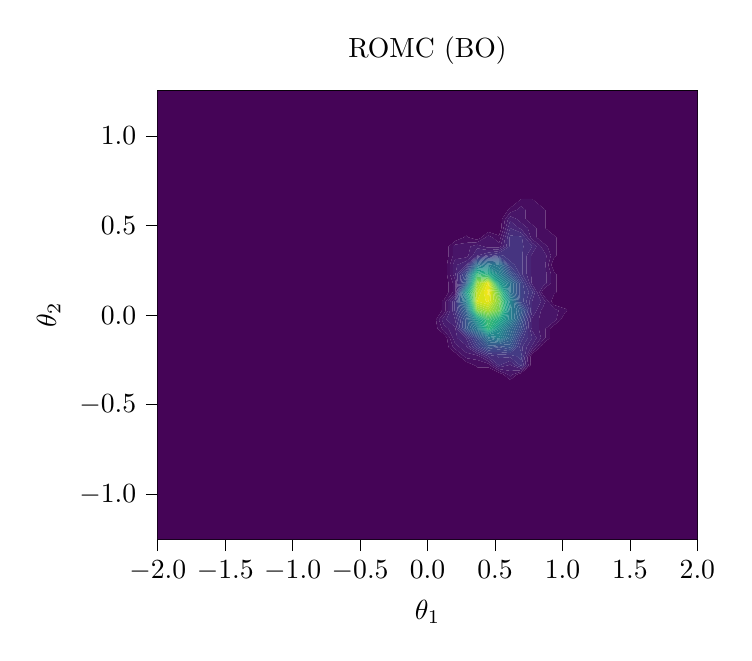
\begin{tikzpicture}

\definecolor{color0}{rgb}{0.269944,0.014625,0.341379}
\definecolor{color1}{rgb}{0.277018,0.050344,0.375715}
\definecolor{color2}{rgb}{0.281446,0.08432,0.407414}
\definecolor{color3}{rgb}{0.283197,0.11568,0.436115}
\definecolor{color4}{rgb}{0.28229,0.145912,0.46151}
\definecolor{color5}{rgb}{0.278826,0.17549,0.483397}
\definecolor{color6}{rgb}{0.273006,0.20452,0.501721}
\definecolor{color7}{rgb}{0.265145,0.232956,0.516599}
\definecolor{color8}{rgb}{0.255645,0.260703,0.528312}
\definecolor{color9}{rgb}{0.244972,0.287675,0.53726}
\definecolor{color10}{rgb}{0.233603,0.313828,0.543914}
\definecolor{color11}{rgb}{0.221989,0.339161,0.548752}
\definecolor{color12}{rgb}{0.210503,0.363727,0.552206}
\definecolor{color13}{rgb}{0.19943,0.387607,0.554642}
\definecolor{color14}{rgb}{0.188923,0.41091,0.556326}
\definecolor{color15}{rgb}{0.179019,0.433756,0.55743}
\definecolor{color16}{rgb}{0.169646,0.456262,0.55803}
\definecolor{color17}{rgb}{0.160665,0.47854,0.558115}
\definecolor{color18}{rgb}{0.151918,0.500685,0.557587}
\definecolor{color19}{rgb}{0.143343,0.522773,0.556295}
\definecolor{color20}{rgb}{0.135066,0.544853,0.554029}
\definecolor{color21}{rgb}{0.127568,0.566949,0.550556}
\definecolor{color22}{rgb}{0.122606,0.585371,0.546557}
\definecolor{color23}{rgb}{0.119512,0.607464,0.540218}
\definecolor{color24}{rgb}{0.12138,0.629492,0.531973}
\definecolor{color25}{rgb}{0.130067,0.651384,0.521608}
\definecolor{color26}{rgb}{0.146616,0.67305,0.508936}
\definecolor{color27}{rgb}{0.170948,0.694384,0.493803}
\definecolor{color28}{rgb}{0.202219,0.715272,0.476084}
\definecolor{color29}{rgb}{0.239374,0.735588,0.455688}
\definecolor{color30}{rgb}{0.281477,0.755203,0.432552}
\definecolor{color31}{rgb}{0.327796,0.77398,0.40664}
\definecolor{color32}{rgb}{0.377779,0.791781,0.377939}
\definecolor{color33}{rgb}{0.430983,0.808473,0.346476}
\definecolor{color34}{rgb}{0.487026,0.823929,0.312321}
\definecolor{color35}{rgb}{0.545524,0.838039,0.275626}
\definecolor{color36}{rgb}{0.606045,0.850733,0.236712}
\definecolor{color37}{rgb}{0.668054,0.861999,0.196293}
\definecolor{color38}{rgb}{0.730889,0.871916,0.156029}
\definecolor{color39}{rgb}{0.79376,0.880678,0.120005}
\definecolor{color40}{rgb}{0.85581,0.888601,0.097452}
\definecolor{color41}{rgb}{0.916242,0.896091,0.100717}
\definecolor{color42}{rgb}{0.974417,0.90359,0.130215}

\begin{axis}[
tick align=outside,
tick pos=left,
title={ROMC (BO)},
x grid style={white!69.0196078431373!black},
xlabel={\(\displaystyle \theta_1\)},
xmin=-2, xmax=2,
xtick style={color=black},
xtick={-2,-1.5,-1,-0.5,0,0.5,1,1.5,2},
xticklabels={
  \(\displaystyle {\ensuremath{-}2.0}\),
  \(\displaystyle {\ensuremath{-}1.5}\),
  \(\displaystyle {\ensuremath{-}1.0}\),
  \(\displaystyle {\ensuremath{-}0.5}\),
  \(\displaystyle {0.0}\),
  \(\displaystyle {0.5}\),
  \(\displaystyle {1.0}\),
  \(\displaystyle {1.5}\),
  \(\displaystyle {2.0}\)
},
y grid style={white!69.0196078431373!black},
ylabel={\(\displaystyle \theta_2\)},
ymin=-1.25, ymax=1.25,
ytick style={color=black},
ytick={-1.5,-1,-0.5,0,0.5,1,1.5},
yticklabels={
  \(\displaystyle {\ensuremath{-}1.5}\),
  \(\displaystyle {\ensuremath{-}1.0}\),
  \(\displaystyle {\ensuremath{-}0.5}\),
  \(\displaystyle {0.0}\),
  \(\displaystyle {0.5}\),
  \(\displaystyle {1.0}\),
  \(\displaystyle {1.5}\)
}
]
\addplot [draw=none, fill=color0]
table{%
x  y
-1.91836734693878 -1.25
-1.83673469387755 -1.25
-1.75510204081633 -1.25
-1.6734693877551 -1.25
-1.59183673469388 -1.25
-1.51020408163265 -1.25
-1.42857142857143 -1.25
-1.3469387755102 -1.25
-1.26530612244898 -1.25
-1.18367346938776 -1.25
-1.10204081632653 -1.25
-1.02040816326531 -1.25
-0.938775510204082 -1.25
-0.857142857142857 -1.25
-0.775510204081633 -1.25
-0.693877551020408 -1.25
-0.612244897959184 -1.25
-0.530612244897959 -1.25
-0.448979591836735 -1.25
-0.36734693877551 -1.25
-0.285714285714286 -1.25
-0.204081632653061 -1.25
-0.122448979591837 -1.25
-0.0408163265306123 -1.25
0.0408163265306123 -1.25
0.122448979591836 -1.25
0.204081632653061 -1.25
0.285714285714286 -1.25
0.36734693877551 -1.25
0.448979591836734 -1.25
0.530612244897959 -1.25
0.612244897959183 -1.25
0.693877551020408 -1.25
0.775510204081633 -1.25
0.857142857142857 -1.25
0.938775510204081 -1.25
1.02040816326531 -1.25
1.10204081632653 -1.25
1.18367346938775 -1.25
1.26530612244898 -1.25
1.3469387755102 -1.25
1.42857142857143 -1.25
1.51020408163265 -1.25
1.59183673469388 -1.25
1.6734693877551 -1.25
1.75510204081633 -1.25
1.83673469387755 -1.25
1.91836734693878 -1.25
2 -1.25
2 -1.19897959183673
2 -1.14795918367347
2 -1.0969387755102
2 -1.04591836734694
2 -0.994897959183674
2 -0.943877551020408
2 -0.892857142857143
2 -0.841836734693878
2 -0.790816326530612
2 -0.739795918367347
2 -0.688775510204082
2 -0.637755102040816
2 -0.586734693877551
2 -0.535714285714286
2 -0.48469387755102
2 -0.433673469387755
2 -0.38265306122449
2 -0.331632653061224
2 -0.280612244897959
2 -0.229591836734694
2 -0.178571428571429
2 -0.127551020408163
2 -0.0765306122448979
2 -0.0255102040816326
2 0.0255102040816326
2 0.0765306122448979
2 0.127551020408163
2 0.178571428571429
2 0.229591836734694
2 0.280612244897959
2 0.331632653061225
2 0.38265306122449
2 0.433673469387755
2 0.48469387755102
2 0.535714285714286
2 0.586734693877551
2 0.637755102040816
2 0.688775510204082
2 0.739795918367347
2 0.790816326530612
2 0.841836734693878
2 0.892857142857143
2 0.943877551020408
2 0.994897959183674
2 1.04591836734694
2 1.0969387755102
2 1.14795918367347
2 1.19897959183673
2 1.25
1.91836734693878 1.25
1.83673469387755 1.25
1.75510204081633 1.25
1.6734693877551 1.25
1.59183673469388 1.25
1.51020408163265 1.25
1.42857142857143 1.25
1.3469387755102 1.25
1.26530612244898 1.25
1.18367346938775 1.25
1.10204081632653 1.25
1.02040816326531 1.25
0.938775510204081 1.25
0.857142857142857 1.25
0.775510204081633 1.25
0.693877551020408 1.25
0.612244897959183 1.25
0.530612244897959 1.25
0.448979591836734 1.25
0.36734693877551 1.25
0.285714285714286 1.25
0.204081632653061 1.25
0.122448979591836 1.25
0.0408163265306123 1.25
-0.0408163265306123 1.25
-0.122448979591837 1.25
-0.204081632653061 1.25
-0.285714285714286 1.25
-0.36734693877551 1.25
-0.448979591836735 1.25
-0.530612244897959 1.25
-0.612244897959184 1.25
-0.693877551020408 1.25
-0.775510204081633 1.25
-0.857142857142857 1.25
-0.938775510204082 1.25
-1.02040816326531 1.25
-1.10204081632653 1.25
-1.18367346938776 1.25
-1.26530612244898 1.25
-1.3469387755102 1.25
-1.42857142857143 1.25
-1.51020408163265 1.25
-1.59183673469388 1.25
-1.6734693877551 1.25
-1.75510204081633 1.25
-1.83673469387755 1.25
-1.91836734693878 1.25
-2 1.25
-2 1.19897959183673
-2 1.14795918367347
-2 1.0969387755102
-2 1.04591836734694
-2 0.994897959183674
-2 0.943877551020408
-2 0.892857142857143
-2 0.841836734693878
-2 0.790816326530612
-2 0.739795918367347
-2 0.688775510204082
-2 0.637755102040816
-2 0.586734693877551
-2 0.535714285714286
-2 0.48469387755102
-2 0.433673469387755
-2 0.38265306122449
-2 0.331632653061225
-2 0.280612244897959
-2 0.229591836734694
-2 0.178571428571429
-2 0.127551020408163
-2 0.0765306122448979
-2 0.0255102040816326
-2 -0.0255102040816326
-2 -0.0765306122448979
-2 -0.127551020408163
-2 -0.178571428571429
-2 -0.229591836734694
-2 -0.280612244897959
-2 -0.331632653061224
-2 -0.38265306122449
-2 -0.433673469387755
-2 -0.48469387755102
-2 -0.535714285714286
-2 -0.586734693877551
-2 -0.637755102040816
-2 -0.688775510204082
-2 -0.739795918367347
-2 -0.790816326530612
-2 -0.841836734693878
-2 -0.892857142857143
-2 -0.943877551020408
-2 -0.994897959183674
-2 -1.04591836734694
-2 -1.0969387755102
-2 -1.14795918367347
-2 -1.19897959183673
-2 -1.25
-1.91836734693878 -1.25

0.563265306122449 -0.331632653061224
0.530612244897959 -0.321428571428571
0.448979591836734 -0.290816326530612
0.36734693877551 -0.290816326530612
0.351020408163265 -0.280612244897959
0.285714285714286 -0.260204081632653
0.236734693877551 -0.229591836734694
0.204081632653061 -0.209183673469388
0.155102040816326 -0.178571428571429
0.14421768707483 -0.127551020408163
0.122448979591836 -0.107142857142857
0.073469387755102 -0.0765306122448979
0.0625850340136054 -0.0255102040816326
0.106122448979592 0.0255102040816326
0.106122448979592 0.0765306122448979
0.122448979591836 0.086734693877551
0.155102040816326 0.127551020408163
0.155102040816326 0.178571428571429
0.14421768707483 0.229591836734694
0.14421768707483 0.280612244897959
0.155102040816326 0.331632653061225
0.155102040816326 0.38265306122449
0.204081632653061 0.413265306122449
0.269387755102041 0.433673469387755
0.285714285714286 0.443877551020408
0.302040816326531 0.433673469387755
0.36734693877551 0.420068027210884
0.4 0.433673469387755
0.448979591836734 0.464285714285714
0.530612244897959 0.443877551020408
0.546938775510204 0.48469387755102
0.552380952380952 0.535714285714286
0.595918367346939 0.586734693877551
0.612244897959183 0.596938775510204
0.677551020408163 0.637755102040816
0.693877551020408 0.647959183673469
0.775510204081633 0.647959183673469
0.791836734693877 0.637755102040816
0.857142857142857 0.596938775510204
0.873469387755102 0.586734693877551
0.873469387755102 0.535714285714286
0.873469387755102 0.48469387755102
0.938775510204081 0.443877551020408
0.955102040816326 0.433673469387755
0.955102040816326 0.38265306122449
0.955102040816326 0.331632653061225
0.938775510204081 0.321428571428572
0.917006802721088 0.280612244897959
0.938775510204081 0.239795918367347
0.955102040816326 0.229591836734694
0.955102040816326 0.178571428571429
0.955102040816326 0.127551020408163
0.938775510204081 0.11734693877551
0.917006802721088 0.0765306122448979
0.938775510204081 0.0561224489795918
1.02040816326531 0.0357142857142857
1.03673469387755 0.0255102040816326
1.02040816326531 0.0153061224489796
0.987755102040816 -0.0255102040816326
0.938775510204081 -0.0561224489795918
0.906122448979591 -0.0765306122448979
0.906122448979591 -0.127551020408163
0.857142857142857 -0.158163265306122
0.835374149659864 -0.178571428571429
0.775510204081633 -0.215986394557823
0.764625850340136 -0.229591836734694
0.762448979591837 -0.280612244897959
0.693877551020408 -0.323469387755102
0.661224489795918 -0.331632653061224
0.612244897959183 -0.362244897959184
0.563265306122449 -0.331632653061224
};
\addplot [draw=none, fill=color1]
table{%
x  y
0.612244897959183 -0.362244897959184
0.661224489795918 -0.331632653061224
0.693877551020408 -0.323469387755102
0.762448979591837 -0.280612244897959
0.764625850340136 -0.229591836734694
0.775510204081633 -0.215986394557823
0.835374149659864 -0.178571428571429
0.857142857142857 -0.158163265306122
0.906122448979591 -0.127551020408163
0.906122448979591 -0.0765306122448979
0.938775510204081 -0.0561224489795918
0.987755102040816 -0.0255102040816326
1.02040816326531 0.0153061224489796
1.03673469387755 0.0255102040816326
1.02040816326531 0.0357142857142857
0.938775510204081 0.0561224489795918
0.917006802721088 0.0765306122448979
0.938775510204081 0.11734693877551
0.955102040816326 0.127551020408163
0.955102040816326 0.178571428571429
0.955102040816326 0.229591836734694
0.938775510204081 0.239795918367347
0.917006802721088 0.280612244897959
0.938775510204081 0.321428571428572
0.955102040816326 0.331632653061225
0.955102040816326 0.38265306122449
0.955102040816326 0.433673469387755
0.938775510204081 0.443877551020408
0.873469387755102 0.48469387755102
0.873469387755102 0.535714285714286
0.873469387755102 0.586734693877551
0.857142857142857 0.596938775510204
0.791836734693877 0.637755102040816
0.775510204081633 0.647959183673469
0.693877551020408 0.647959183673469
0.677551020408163 0.637755102040816
0.612244897959183 0.596938775510204
0.595918367346939 0.586734693877551
0.552380952380952 0.535714285714286
0.546938775510204 0.48469387755102
0.530612244897959 0.443877551020408
0.448979591836734 0.464285714285714
0.4 0.433673469387755
0.36734693877551 0.420068027210884
0.302040816326531 0.433673469387755
0.285714285714286 0.443877551020408
0.269387755102041 0.433673469387755
0.204081632653061 0.413265306122449
0.155102040816326 0.38265306122449
0.155102040816326 0.331632653061225
0.14421768707483 0.280612244897959
0.14421768707483 0.229591836734694
0.155102040816326 0.178571428571429
0.155102040816326 0.127551020408163
0.122448979591836 0.086734693877551
0.106122448979592 0.0765306122448979
0.106122448979592 0.0255102040816326
0.0625850340136054 -0.0255102040816326
0.073469387755102 -0.0765306122448979
0.122448979591836 -0.107142857142857
0.14421768707483 -0.127551020408163
0.155102040816326 -0.178571428571429
0.204081632653061 -0.209183673469388
0.236734693877551 -0.229591836734694
0.285714285714286 -0.260204081632653
0.351020408163265 -0.280612244897959
0.36734693877551 -0.290816326530612
0.448979591836734 -0.290816326530612
0.530612244897959 -0.321428571428571
0.563265306122449 -0.331632653061224
0.612244897959183 -0.362244897959184

0.595918367346939 -0.331632653061224
0.530612244897959 -0.311224489795918
0.465306122448979 -0.280612244897959
0.448979591836734 -0.270408163265306
0.36734693877551 -0.25
0.285714285714286 -0.239795918367347
0.269387755102041 -0.229591836734694
0.204081632653061 -0.188775510204082
0.187755102040816 -0.178571428571429
0.165986394557823 -0.127551020408163
0.122448979591836 -0.0867346938775509
0.106122448979592 -0.0765306122448979
0.0843537414965985 -0.0255102040816326
0.122448979591836 0.010204081632653
0.13469387755102 0.0255102040816326
0.13469387755102 0.0765306122448979
0.187755102040816 0.127551020408163
0.187755102040816 0.178571428571429
0.165986394557823 0.229591836734694
0.165986394557823 0.280612244897959
0.187755102040816 0.331632653061225
0.187755102040816 0.38265306122449
0.204081632653061 0.392857142857143
0.285714285714286 0.403061224489796
0.36734693877551 0.406462585034014
0.432653061224489 0.433673469387755
0.448979591836734 0.443877551020408
0.481632653061224 0.433673469387755
0.530612244897959 0.403061224489796
0.542857142857143 0.433673469387755
0.563265306122449 0.48469387755102
0.574149659863945 0.535714285714286
0.612244897959183 0.571428571428571
0.661224489795918 0.586734693877551
0.693877551020408 0.607142857142857
0.726530612244898 0.586734693877551
0.726530612244898 0.535714285714286
0.775510204081633 0.505102040816326
0.808163265306122 0.48469387755102
0.808163265306122 0.433673469387755
0.857142857142857 0.403061224489796
0.889795918367347 0.38265306122449
0.914285714285714 0.331632653061225
0.895238095238095 0.280612244897959
0.914285714285714 0.229591836734694
0.914285714285714 0.178571428571429
0.857142857142857 0.142857142857143
0.844897959183673 0.127551020408163
0.857142857142857 0.112244897959184
0.895238095238095 0.0765306122448979
0.938775510204081 0.0357142857142857
0.971428571428571 0.0255102040816326
0.955102040816326 -0.0255102040816326
0.938775510204081 -0.0357142857142857
0.873469387755102 -0.0765306122448979
0.873469387755102 -0.127551020408163
0.857142857142857 -0.137755102040816
0.813605442176871 -0.178571428571429
0.775510204081633 -0.202380952380952
0.753741496598639 -0.229591836734694
0.749387755102041 -0.280612244897959
0.693877551020408 -0.31530612244898
0.628571428571428 -0.331632653061224
0.612244897959183 -0.341836734693878
0.595918367346939 -0.331632653061224
};
\addplot [draw=none, fill=color2]
table{%
x  y
0.612244897959183 -0.341836734693878
0.628571428571428 -0.331632653061224
0.693877551020408 -0.31530612244898
0.749387755102041 -0.280612244897959
0.753741496598639 -0.229591836734694
0.775510204081633 -0.202380952380952
0.813605442176871 -0.178571428571429
0.857142857142857 -0.137755102040816
0.873469387755102 -0.127551020408163
0.873469387755102 -0.0765306122448979
0.938775510204081 -0.0357142857142857
0.955102040816326 -0.0255102040816326
0.971428571428571 0.0255102040816326
0.938775510204081 0.0357142857142857
0.895238095238095 0.0765306122448979
0.857142857142857 0.112244897959184
0.844897959183673 0.127551020408163
0.857142857142857 0.142857142857143
0.914285714285714 0.178571428571429
0.914285714285714 0.229591836734694
0.895238095238095 0.280612244897959
0.914285714285714 0.331632653061225
0.889795918367347 0.38265306122449
0.857142857142857 0.403061224489796
0.808163265306122 0.433673469387755
0.808163265306122 0.48469387755102
0.775510204081633 0.505102040816326
0.726530612244898 0.535714285714286
0.726530612244898 0.586734693877551
0.693877551020408 0.607142857142857
0.661224489795918 0.586734693877551
0.612244897959183 0.571428571428571
0.574149659863945 0.535714285714286
0.563265306122449 0.48469387755102
0.542857142857143 0.433673469387755
0.530612244897959 0.403061224489796
0.481632653061224 0.433673469387755
0.448979591836734 0.443877551020408
0.432653061224489 0.433673469387755
0.36734693877551 0.406462585034014
0.285714285714286 0.403061224489796
0.204081632653061 0.392857142857143
0.187755102040816 0.38265306122449
0.187755102040816 0.331632653061225
0.165986394557823 0.280612244897959
0.165986394557823 0.229591836734694
0.187755102040816 0.178571428571429
0.187755102040816 0.127551020408163
0.13469387755102 0.0765306122448979
0.13469387755102 0.0255102040816326
0.122448979591836 0.010204081632653
0.0843537414965985 -0.0255102040816326
0.106122448979592 -0.0765306122448979
0.122448979591836 -0.0867346938775509
0.165986394557823 -0.127551020408163
0.187755102040816 -0.178571428571429
0.204081632653061 -0.188775510204082
0.269387755102041 -0.229591836734694
0.285714285714286 -0.239795918367347
0.36734693877551 -0.25
0.448979591836734 -0.270408163265306
0.465306122448979 -0.280612244897959
0.530612244897959 -0.311224489795918
0.595918367346939 -0.331632653061224
0.612244897959183 -0.341836734693878

0.487074829931972 -0.280612244897959
0.448979591836734 -0.256802721088435
0.383673469387755 -0.229591836734694
0.36734693877551 -0.224489795918367
0.285714285714286 -0.209183673469388
0.236734693877551 -0.178571428571429
0.204081632653061 -0.158163265306122
0.187755102040816 -0.127551020408163
0.155102040816326 -0.0765306122448979
0.122448979591836 -0.0561224489795918
0.106122448979592 -0.0255102040816326
0.122448979591836 -0.0102040816326531
0.151020408163265 0.0255102040816326
0.151020408163265 0.0765306122448979
0.204081632653061 0.120748299319728
0.206122448979592 0.127551020408163
0.208163265306122 0.178571428571429
0.204081632653061 0.198979591836735
0.187755102040816 0.229591836734694
0.187755102040816 0.280612244897959
0.204081632653061 0.311224489795918
0.285714285714286 0.321428571428572
0.302040816326531 0.331632653061225
0.318367346938775 0.38265306122449
0.36734693877551 0.392857142857143
0.416326530612245 0.38265306122449
0.448979591836734 0.375850340136055
0.530612244897959 0.377551020408163
0.541496598639456 0.38265306122449
0.559183673469387 0.433673469387755
0.579591836734694 0.48469387755102
0.595918367346939 0.535714285714286
0.612244897959183 0.551020408163265
0.661224489795918 0.535714285714286
0.693877551020408 0.51530612244898
0.742857142857143 0.48469387755102
0.764625850340136 0.433673469387755
0.775510204081633 0.423469387755102
0.840816326530612 0.38265306122449
0.857142857142857 0.362244897959184
0.881632653061224 0.331632653061225
0.873469387755102 0.280612244897959
0.881632653061224 0.229591836734694
0.881632653061224 0.178571428571429
0.857142857142857 0.163265306122449
0.828571428571428 0.127551020408163
0.857142857142857 0.0918367346938775
0.873469387755102 0.0765306122448979
0.857142857142857 0.0459183673469387
0.840816326530612 0.0255102040816326
0.824489795918367 -0.0255102040816326
0.824489795918367 -0.0765306122448979
0.840816326530612 -0.127551020408163
0.791836734693877 -0.178571428571429
0.775510204081633 -0.188775510204082
0.742857142857143 -0.229591836734694
0.736326530612245 -0.280612244897959
0.693877551020408 -0.307142857142857
0.612244897959183 -0.311224489795918
0.530612244897959 -0.301020408163265
0.487074829931972 -0.280612244897959
};
\addplot [draw=none, fill=color3]
table{%
x  y
0.530612244897959 -0.301020408163265
0.612244897959183 -0.311224489795918
0.693877551020408 -0.307142857142857
0.736326530612245 -0.280612244897959
0.742857142857143 -0.229591836734694
0.775510204081633 -0.188775510204082
0.791836734693877 -0.178571428571429
0.840816326530612 -0.127551020408163
0.824489795918367 -0.0765306122448979
0.824489795918367 -0.0255102040816326
0.840816326530612 0.0255102040816326
0.857142857142857 0.0459183673469387
0.873469387755102 0.0765306122448979
0.857142857142857 0.0918367346938775
0.828571428571428 0.127551020408163
0.857142857142857 0.163265306122449
0.881632653061224 0.178571428571429
0.881632653061224 0.229591836734694
0.873469387755102 0.280612244897959
0.881632653061224 0.331632653061225
0.857142857142857 0.362244897959184
0.840816326530612 0.38265306122449
0.775510204081633 0.423469387755102
0.764625850340136 0.433673469387755
0.742857142857143 0.48469387755102
0.693877551020408 0.51530612244898
0.661224489795918 0.535714285714286
0.612244897959183 0.551020408163265
0.595918367346939 0.535714285714286
0.579591836734694 0.48469387755102
0.559183673469387 0.433673469387755
0.541496598639456 0.38265306122449
0.530612244897959 0.377551020408163
0.448979591836734 0.375850340136054
0.416326530612245 0.38265306122449
0.36734693877551 0.392857142857143
0.318367346938775 0.38265306122449
0.302040816326531 0.331632653061225
0.285714285714286 0.321428571428572
0.204081632653061 0.311224489795918
0.187755102040816 0.280612244897959
0.187755102040816 0.229591836734694
0.204081632653061 0.198979591836735
0.208163265306122 0.178571428571429
0.206122448979592 0.127551020408163
0.204081632653061 0.120748299319728
0.151020408163265 0.0765306122448979
0.151020408163265 0.0255102040816326
0.122448979591836 -0.0102040816326531
0.106122448979592 -0.0255102040816326
0.122448979591836 -0.0561224489795918
0.155102040816326 -0.0765306122448979
0.187755102040816 -0.127551020408163
0.204081632653061 -0.158163265306122
0.236734693877551 -0.178571428571429
0.285714285714286 -0.209183673469388
0.36734693877551 -0.224489795918367
0.383673469387755 -0.229591836734694
0.448979591836734 -0.256802721088435
0.487074829931972 -0.280612244897959
0.530612244897959 -0.301020408163265

0.508843537414966 -0.280612244897959
0.448979591836734 -0.243197278911565
0.416326530612245 -0.229591836734694
0.36734693877551 -0.214285714285714
0.291156462585034 -0.178571428571429
0.285714285714286 -0.168367346938776
0.220408163265306 -0.127551020408163
0.206802721088435 -0.0765306122448979
0.204081632653061 -0.0663265306122448
0.138775510204081 -0.0255102040816326
0.16734693877551 0.0255102040816326
0.16734693877551 0.0765306122448979
0.204081632653061 0.107142857142857
0.210204081632653 0.127551020408163
0.216326530612245 0.178571428571429
0.20734693877551 0.229591836734694
0.220408163265306 0.280612244897959
0.285714285714286 0.301020408163265
0.33469387755102 0.331632653061225
0.36734693877551 0.372448979591837
0.448979591836734 0.362244897959184
0.530612244897959 0.36734693877551
0.563265306122449 0.38265306122449
0.575510204081632 0.433673469387755
0.595918367346939 0.48469387755102
0.612244897959183 0.525510204081633
0.677551020408163 0.48469387755102
0.693877551020408 0.479591836734694
0.742857142857143 0.433673469387755
0.775510204081633 0.403061224489796
0.808163265306122 0.38265306122449
0.775510204081633 0.341836734693878
0.76734693877551 0.331632653061225
0.76734693877551 0.280612244897959
0.76734693877551 0.229591836734694
0.771428571428571 0.178571428571429
0.775510204081633 0.173469387755102
0.812244897959183 0.127551020408163
0.840816326530612 0.0765306122448979
0.808163265306122 0.0255102040816326
0.775510204081633 -0.0153061224489796
0.772789115646259 -0.0255102040816326
0.772244897959184 -0.0765306122448979
0.775510204081633 -0.0867346938775509
0.808163265306122 -0.127551020408163
0.775510204081633 -0.168367346938776
0.76734693877551 -0.178571428571429
0.731972789115646 -0.229591836734694
0.723265306122449 -0.280612244897959
0.693877551020408 -0.298979591836735
0.620408163265306 -0.280612244897959
0.612244897959183 -0.275510204081633
0.595918367346938 -0.280612244897959
0.530612244897959 -0.290816326530612
0.508843537414966 -0.280612244897959
};
\addplot [draw=none, fill=color4]
table{%
x  y
0.530612244897959 -0.290816326530612
0.595918367346938 -0.280612244897959
0.612244897959183 -0.275510204081633
0.620408163265306 -0.280612244897959
0.693877551020408 -0.298979591836735
0.723265306122449 -0.280612244897959
0.731972789115646 -0.229591836734694
0.76734693877551 -0.178571428571429
0.775510204081633 -0.168367346938776
0.808163265306122 -0.127551020408163
0.775510204081633 -0.0867346938775509
0.772244897959184 -0.0765306122448979
0.772789115646259 -0.0255102040816326
0.775510204081633 -0.0153061224489796
0.808163265306122 0.0255102040816326
0.840816326530612 0.0765306122448979
0.812244897959183 0.127551020408163
0.775510204081633 0.173469387755102
0.771428571428571 0.178571428571429
0.76734693877551 0.229591836734694
0.76734693877551 0.280612244897959
0.76734693877551 0.331632653061225
0.775510204081633 0.341836734693878
0.808163265306122 0.38265306122449
0.775510204081633 0.403061224489796
0.742857142857143 0.433673469387755
0.693877551020408 0.479591836734694
0.677551020408163 0.48469387755102
0.612244897959183 0.525510204081633
0.595918367346939 0.48469387755102
0.575510204081632 0.433673469387755
0.563265306122449 0.38265306122449
0.530612244897959 0.36734693877551
0.448979591836734 0.362244897959184
0.36734693877551 0.372448979591837
0.33469387755102 0.331632653061225
0.285714285714286 0.301020408163265
0.220408163265306 0.280612244897959
0.20734693877551 0.229591836734694
0.216326530612245 0.178571428571429
0.210204081632653 0.127551020408163
0.204081632653061 0.107142857142857
0.16734693877551 0.0765306122448979
0.16734693877551 0.0255102040816326
0.138775510204081 -0.0255102040816326
0.204081632653061 -0.0663265306122448
0.206802721088435 -0.0765306122448979
0.220408163265306 -0.127551020408163
0.285714285714286 -0.168367346938776
0.291156462585034 -0.178571428571429
0.36734693877551 -0.214285714285714
0.416326530612245 -0.229591836734694
0.448979591836734 -0.243197278911565
0.508843537414966 -0.280612244897959
0.530612244897959 -0.290816326530612

0.653061224489796 -0.280612244897959
0.612244897959183 -0.255102040816326
0.530612244897959 -0.280612244897959
0.448979591836734 -0.229591836734694
0.36734693877551 -0.204081632653061
0.312925170068027 -0.178571428571429
0.285714285714286 -0.127551020408163
0.217687074829932 -0.0765306122448979
0.204081632653061 -0.0255102040816326
0.183673469387755 0.0255102040816326
0.183673469387755 0.0765306122448979
0.204081632653061 0.0935374149659864
0.214285714285714 0.127551020408163
0.224489795918367 0.178571428571429
0.220408163265306 0.229591836734694
0.285714285714286 0.280612244897959
0.36734693877551 0.331632653061225
0.36734693877551 0.331632653061225
0.448979591836734 0.348639455782313
0.530612244897959 0.357142857142857
0.585034013605442 0.38265306122449
0.591836734693877 0.433673469387755
0.612244897959183 0.48469387755102
0.693877551020408 0.459183673469388
0.72108843537415 0.433673469387755
0.775510204081633 0.38265306122449
0.73469387755102 0.331632653061225
0.73469387755102 0.280612244897959
0.73469387755102 0.229591836734694
0.755102040816326 0.178571428571429
0.775510204081633 0.153061224489796
0.795918367346939 0.127551020408163
0.775510204081633 0.0765306122448979
0.775510204081633 0.0255102040816326
0.761904761904762 -0.0255102040816326
0.759183673469388 -0.0765306122448979
0.775510204081633 -0.127551020408163
0.73469387755102 -0.178571428571429
0.72108843537415 -0.229591836734694
0.710204081632653 -0.280612244897959
0.693877551020408 -0.290816326530612
0.653061224489796 -0.280612244897959
};
\addplot [draw=none, fill=color5]
table{%
x  y
0.693877551020408 -0.290816326530612
0.710204081632653 -0.280612244897959
0.72108843537415 -0.229591836734694
0.73469387755102 -0.178571428571429
0.775510204081633 -0.127551020408163
0.759183673469388 -0.0765306122448979
0.761904761904762 -0.0255102040816326
0.775510204081633 0.0255102040816326
0.775510204081633 0.0765306122448979
0.795918367346939 0.127551020408163
0.775510204081633 0.153061224489796
0.755102040816326 0.178571428571429
0.73469387755102 0.229591836734694
0.73469387755102 0.280612244897959
0.73469387755102 0.331632653061225
0.775510204081633 0.38265306122449
0.72108843537415 0.433673469387755
0.693877551020408 0.459183673469388
0.612244897959183 0.48469387755102
0.591836734693877 0.433673469387755
0.585034013605442 0.38265306122449
0.530612244897959 0.357142857142857
0.448979591836734 0.348639455782313
0.36734693877551 0.331632653061225
0.36734693877551 0.331632653061225
0.285714285714286 0.280612244897959
0.220408163265306 0.229591836734694
0.224489795918367 0.178571428571429
0.214285714285714 0.127551020408163
0.204081632653061 0.0935374149659864
0.183673469387755 0.0765306122448979
0.183673469387755 0.0255102040816326
0.204081632653061 -0.0255102040816326
0.217687074829932 -0.0765306122448979
0.285714285714286 -0.127551020408163
0.312925170068027 -0.178571428571429
0.36734693877551 -0.204081632653061
0.448979591836734 -0.229591836734694
0.530612244897959 -0.280612244897959
0.612244897959183 -0.255102040816326
0.653061224489796 -0.280612244897959
0.693877551020408 -0.290816326530612

0.685714285714286 -0.280612244897959
0.612244897959183 -0.23469387755102
0.530612244897959 -0.239795918367347
0.514285714285714 -0.229591836734694
0.448979591836734 -0.221428571428571
0.36734693877551 -0.193877551020408
0.33469387755102 -0.178571428571429
0.302040816326531 -0.127551020408163
0.285714285714286 -0.119387755102041
0.228571428571428 -0.0765306122448979
0.217142857142857 -0.0255102040816326
0.204081632653061 0.0153061224489796
0.2 0.0255102040816326
0.2 0.0765306122448979
0.204081632653061 0.0799319727891156
0.218367346938775 0.127551020408163
0.23265306122449 0.178571428571429
0.233469387755102 0.229591836734694
0.285714285714286 0.270408163265306
0.293877551020408 0.280612244897959
0.36734693877551 0.326530612244898
0.43265306122449 0.331632653061225
0.448979591836734 0.335034013605442
0.530612244897959 0.346938775510204
0.606802721088435 0.38265306122449
0.608163265306122 0.433673469387755
0.612244897959183 0.443877551020408
0.693877551020408 0.438775510204082
0.699319727891156 0.433673469387755
0.710204081632653 0.38265306122449
0.70204081632653 0.331632653061225
0.70204081632653 0.280612244897959
0.70204081632653 0.229591836734694
0.738775510204082 0.178571428571429
0.775510204081633 0.13265306122449
0.779591836734694 0.127551020408163
0.775510204081633 0.11734693877551
0.75374149659864 0.0765306122448979
0.764625850340136 0.0255102040816326
0.751020408163265 -0.0255102040816326
0.746122448979592 -0.0765306122448979
0.742857142857143 -0.127551020408163
0.70204081632653 -0.178571428571429
0.710204081632653 -0.229591836734694
0.697142857142857 -0.280612244897959
0.693877551020408 -0.28265306122449
0.685714285714286 -0.280612244897959
};
\addplot [draw=none, fill=color6]
table{%
x  y
0.693877551020408 -0.28265306122449
0.697142857142857 -0.280612244897959
0.710204081632653 -0.229591836734694
0.70204081632653 -0.178571428571429
0.742857142857143 -0.127551020408163
0.746122448979592 -0.0765306122448979
0.751020408163265 -0.0255102040816326
0.764625850340136 0.0255102040816326
0.753741496598639 0.0765306122448979
0.775510204081633 0.11734693877551
0.779591836734694 0.127551020408163
0.775510204081633 0.13265306122449
0.738775510204082 0.178571428571429
0.70204081632653 0.229591836734694
0.70204081632653 0.280612244897959
0.70204081632653 0.331632653061225
0.710204081632653 0.38265306122449
0.699319727891156 0.433673469387755
0.693877551020408 0.438775510204082
0.612244897959183 0.443877551020408
0.608163265306122 0.433673469387755
0.606802721088435 0.38265306122449
0.530612244897959 0.346938775510204
0.448979591836734 0.335034013605442
0.43265306122449 0.331632653061225
0.36734693877551 0.326530612244898
0.293877551020408 0.280612244897959
0.285714285714286 0.270408163265306
0.233469387755102 0.229591836734694
0.23265306122449 0.178571428571429
0.218367346938775 0.127551020408163
0.204081632653061 0.0799319727891156
0.2 0.0765306122448979
0.2 0.0255102040816326
0.204081632653061 0.0153061224489796
0.217142857142857 -0.0255102040816326
0.228571428571428 -0.0765306122448979
0.285714285714286 -0.119387755102041
0.302040816326531 -0.127551020408163
0.33469387755102 -0.178571428571429
0.36734693877551 -0.193877551020408
0.448979591836734 -0.221428571428571
0.514285714285714 -0.229591836734694
0.530612244897959 -0.239795918367347
0.612244897959183 -0.23469387755102
0.685714285714286 -0.280612244897959
0.693877551020408 -0.28265306122449

0.661224489795918 -0.229591836734694
0.612244897959183 -0.221938775510204
0.530612244897959 -0.219387755102041
0.448979591836734 -0.213265306122449
0.36734693877551 -0.183673469387755
0.356462585034014 -0.178571428571429
0.318367346938775 -0.127551020408163
0.285714285714286 -0.111224489795918
0.239455782312925 -0.0765306122448979
0.230204081632653 -0.0255102040816326
0.212244897959183 0.0255102040816326
0.208979591836734 0.0765306122448979
0.222448979591837 0.127551020408163
0.240816326530612 0.178571428571429
0.246530612244898 0.229591836734694
0.285714285714286 0.260204081632653
0.302040816326531 0.280612244897959
0.36734693877551 0.321428571428572
0.448979591836734 0.328231292517007
0.497959183673469 0.331632653061225
0.530612244897959 0.336734693877551
0.563265306122449 0.331632653061225
0.612244897959183 0.301020408163265
0.644897959183673 0.280612244897959
0.681632653061224 0.229591836734694
0.693877551020408 0.214285714285714
0.722448979591837 0.178571428571429
0.751020408163265 0.127551020408163
0.731972789115646 0.0765306122448979
0.753741496598639 0.0255102040816326
0.740136054421769 -0.0255102040816326
0.733061224489796 -0.0765306122448979
0.710204081632653 -0.127551020408163
0.693877551020408 -0.147959183673469
0.681632653061224 -0.178571428571429
0.693877551020408 -0.209183673469388
0.699319727891156 -0.229591836734694
0.693877551020408 -0.25
0.661224489795918 -0.229591836734694
};
\addplot [draw=none, fill=color7]
table{%
x  y
0.693877551020408 -0.25
0.699319727891156 -0.229591836734694
0.693877551020408 -0.209183673469388
0.681632653061224 -0.178571428571429
0.693877551020408 -0.147959183673469
0.710204081632653 -0.127551020408163
0.733061224489796 -0.0765306122448979
0.740136054421769 -0.0255102040816326
0.753741496598639 0.0255102040816326
0.731972789115646 0.0765306122448979
0.751020408163265 0.127551020408163
0.722448979591837 0.178571428571429
0.693877551020408 0.214285714285714
0.681632653061224 0.229591836734694
0.644897959183673 0.280612244897959
0.612244897959183 0.301020408163265
0.563265306122449 0.331632653061225
0.530612244897959 0.336734693877551
0.497959183673469 0.331632653061225
0.448979591836734 0.328231292517007
0.36734693877551 0.321428571428572
0.302040816326531 0.280612244897959
0.285714285714286 0.260204081632653
0.246530612244898 0.229591836734694
0.240816326530612 0.178571428571429
0.222448979591837 0.127551020408163
0.208979591836735 0.0765306122448979
0.212244897959183 0.0255102040816326
0.230204081632653 -0.0255102040816326
0.239455782312925 -0.0765306122448979
0.285714285714286 -0.111224489795918
0.318367346938775 -0.127551020408163
0.356462585034014 -0.178571428571429
0.36734693877551 -0.183673469387755
0.448979591836734 -0.213265306122449
0.530612244897959 -0.219387755102041
0.612244897959183 -0.221938775510204
0.661224489795918 -0.229591836734694
0.693877551020408 -0.25

0.378231292517007 -0.178571428571429
0.36734693877551 -0.168367346938775
0.33469387755102 -0.127551020408163
0.285714285714286 -0.103061224489796
0.250340136054422 -0.0765306122448979
0.243265306122449 -0.0255102040816326
0.22312925170068 0.0255102040816326
0.215510204081632 0.0765306122448979
0.226530612244898 0.127551020408163
0.248979591836735 0.178571428571429
0.259591836734694 0.229591836734694
0.285714285714286 0.25
0.310204081632653 0.280612244897959
0.36734693877551 0.316326530612245
0.448979591836734 0.323696145124717
0.530612244897959 0.328717201166181
0.607580174927114 0.280612244897959
0.612244897959183 0.273809523809524
0.665306122448979 0.229591836734694
0.693877551020408 0.193877551020408
0.706122448979592 0.178571428571429
0.718367346938775 0.127551020408163
0.710204081632653 0.0765306122448979
0.742857142857143 0.0255102040816326
0.729251700680272 -0.0255102040816326
0.72 -0.0765306122448979
0.693877551020408 -0.11734693877551
0.68734693877551 -0.127551020408163
0.665306122448979 -0.178571428571429
0.612244897959183 -0.211734693877551
0.530612244897959 -0.20578231292517
0.448979591836734 -0.205102040816327
0.378231292517007 -0.178571428571429
};
\addplot [draw=none, fill=color8]
table{%
x  y
0.448979591836734 -0.205102040816327
0.530612244897959 -0.20578231292517
0.612244897959183 -0.211734693877551
0.665306122448979 -0.178571428571429
0.68734693877551 -0.127551020408163
0.693877551020408 -0.11734693877551
0.72 -0.0765306122448979
0.729251700680272 -0.0255102040816326
0.742857142857143 0.0255102040816326
0.710204081632653 0.0765306122448979
0.718367346938775 0.127551020408163
0.706122448979592 0.178571428571429
0.693877551020408 0.193877551020408
0.665306122448979 0.229591836734694
0.612244897959183 0.273809523809524
0.607580174927114 0.280612244897959
0.530612244897959 0.328717201166181
0.448979591836734 0.323696145124717
0.36734693877551 0.316326530612245
0.310204081632653 0.280612244897959
0.285714285714286 0.25
0.259591836734694 0.229591836734694
0.248979591836735 0.178571428571429
0.226530612244898 0.127551020408163
0.215510204081632 0.0765306122448979
0.22312925170068 0.0255102040816326
0.243265306122449 -0.0255102040816326
0.250340136054422 -0.0765306122448979
0.285714285714286 -0.103061224489796
0.33469387755102 -0.127551020408163
0.36734693877551 -0.168367346938775
0.378231292517007 -0.178571428571429
0.448979591836734 -0.205102040816327

0.4 -0.178571428571429
0.36734693877551 -0.147959183673469
0.351020408163265 -0.127551020408163
0.285714285714286 -0.0948979591836734
0.261224489795918 -0.0765306122448979
0.256326530612245 -0.0255102040816326
0.234013605442177 0.0255102040816326
0.22204081632653 0.0765306122448979
0.230612244897959 0.127551020408163
0.257142857142857 0.178571428571429
0.27265306122449 0.229591836734694
0.285714285714286 0.239795918367347
0.318367346938775 0.280612244897959
0.36734693877551 0.311224489795918
0.448979591836734 0.319160997732426
0.530612244897959 0.322886297376093
0.598250728862973 0.280612244897959
0.612244897959183 0.260204081632653
0.648979591836734 0.229591836734694
0.691156462585034 0.178571428571429
0.691156462585034 0.127551020408163
0.692063492063492 0.0765306122448979
0.693877551020408 0.0731292517006802
0.731972789115646 0.0255102040816326
0.718367346938775 -0.0255102040816326
0.706938775510204 -0.0765306122448979
0.693877551020408 -0.096938775510204
0.674285714285714 -0.127551020408163
0.648979591836734 -0.178571428571429
0.612244897959183 -0.201530612244898
0.530612244897959 -0.192176870748299
0.448979591836734 -0.196938775510204
0.4 -0.178571428571429
};
\addplot [draw=none, fill=color9]
table{%
x  y
0.448979591836734 -0.196938775510204
0.530612244897959 -0.192176870748299
0.612244897959183 -0.201530612244898
0.648979591836734 -0.178571428571429
0.674285714285714 -0.127551020408163
0.693877551020408 -0.096938775510204
0.706938775510204 -0.0765306122448979
0.718367346938775 -0.0255102040816326
0.731972789115646 0.0255102040816326
0.693877551020408 0.0731292517006802
0.692063492063492 0.0765306122448979
0.691156462585034 0.127551020408163
0.691156462585034 0.178571428571429
0.648979591836734 0.229591836734694
0.612244897959183 0.260204081632653
0.598250728862973 0.280612244897959
0.530612244897959 0.322886297376093
0.448979591836734 0.319160997732426
0.36734693877551 0.311224489795918
0.318367346938775 0.280612244897959
0.285714285714286 0.239795918367347
0.27265306122449 0.229591836734694
0.257142857142857 0.178571428571429
0.230612244897959 0.127551020408163
0.22204081632653 0.0765306122448979
0.234013605442177 0.0255102040816326
0.256326530612245 -0.0255102040816326
0.261224489795918 -0.0765306122448979
0.285714285714286 -0.0948979591836734
0.351020408163265 -0.127551020408163
0.36734693877551 -0.147959183673469
0.4 -0.178571428571429
0.448979591836734 -0.196938775510204

0.421768707482993 -0.178571428571429
0.36734693877551 -0.127551020408163
0.36734693877551 -0.127551020408163
0.285714285714286 -0.0867346938775509
0.272108843537415 -0.0765306122448979
0.269387755102041 -0.0255102040816326
0.244897959183673 0.0255102040816326
0.228571428571428 0.0765306122448979
0.23469387755102 0.127551020408163
0.265306122448979 0.178571428571429
0.285714285714286 0.229591836734694
0.326530612244898 0.280612244897959
0.36734693877551 0.306122448979592
0.448979591836734 0.314625850340136
0.530612244897959 0.317055393586006
0.588921282798834 0.280612244897959
0.612244897959183 0.246598639455782
0.63265306122449 0.229591836734694
0.680272108843537 0.178571428571429
0.680272108843537 0.127551020408163
0.684807256235827 0.0765306122448979
0.693877551020408 0.0595238095238095
0.72108843537415 0.0255102040816326
0.707482993197279 -0.0255102040816326
0.693877551020408 -0.0765306122448979
0.661224489795918 -0.127551020408163
0.63265306122449 -0.178571428571429
0.612244897959183 -0.191326530612245
0.530612244897959 -0.178571428571429
0.448979591836734 -0.188775510204082
0.421768707482993 -0.178571428571429
};
\addplot [draw=none, fill=color10]
table{%
x  y
0.448979591836734 -0.188775510204082
0.530612244897959 -0.178571428571429
0.612244897959183 -0.191326530612245
0.63265306122449 -0.178571428571429
0.661224489795918 -0.127551020408163
0.693877551020408 -0.0765306122448979
0.707482993197279 -0.0255102040816326
0.72108843537415 0.0255102040816326
0.693877551020408 0.0595238095238095
0.684807256235827 0.0765306122448979
0.680272108843537 0.127551020408163
0.680272108843537 0.178571428571429
0.63265306122449 0.229591836734694
0.612244897959183 0.246598639455782
0.588921282798834 0.280612244897959
0.530612244897959 0.317055393586006
0.448979591836734 0.314625850340136
0.36734693877551 0.306122448979592
0.326530612244898 0.280612244897959
0.285714285714286 0.229591836734694
0.265306122448979 0.178571428571429
0.23469387755102 0.127551020408163
0.228571428571428 0.0765306122448979
0.244897959183673 0.0255102040816326
0.269387755102041 -0.0255102040816326
0.272108843537415 -0.0765306122448979
0.285714285714286 -0.0867346938775509
0.36734693877551 -0.127551020408163
0.36734693877551 -0.127551020408163
0.421768707482993 -0.178571428571429
0.448979591836734 -0.188775510204082

0.443537414965986 -0.178571428571429
0.380408163265306 -0.127551020408163
0.36734693877551 -0.120748299319728
0.285714285714286 -0.0785714285714285
0.282993197278911 -0.0765306122448979
0.282448979591837 -0.0255102040816326
0.25578231292517 0.0255102040816326
0.235102040816326 0.0765306122448979
0.238775510204081 0.127551020408163
0.273469387755102 0.178571428571429
0.285714285714286 0.209183673469388
0.290068027210884 0.229591836734694
0.33469387755102 0.280612244897959
0.36734693877551 0.301020408163265
0.448979591836734 0.310090702947846
0.530612244897959 0.311224489795918
0.579591836734694 0.280612244897959
0.612244897959183 0.232993197278912
0.616326530612245 0.229591836734694
0.669387755102041 0.178571428571429
0.669387755102041 0.127551020408163
0.677551020408163 0.0765306122448979
0.693877551020408 0.0459183673469387
0.710204081632653 0.0255102040816326
0.696598639455782 -0.0255102040816326
0.693877551020408 -0.0357142857142856
0.677551020408163 -0.0765306122448979
0.648163265306122 -0.127551020408163
0.616326530612245 -0.178571428571429
0.612244897959183 -0.181122448979592
0.595918367346939 -0.178571428571429
0.530612244897959 -0.172740524781341
0.465306122448979 -0.178571428571429
0.448979591836734 -0.180612244897959
0.443537414965986 -0.178571428571429
};
\addplot [draw=none, fill=color11]
table{%
x  y
0.448979591836734 -0.180612244897959
0.465306122448979 -0.178571428571429
0.530612244897959 -0.172740524781341
0.595918367346939 -0.178571428571429
0.612244897959183 -0.181122448979592
0.616326530612245 -0.178571428571429
0.648163265306122 -0.127551020408163
0.677551020408163 -0.0765306122448979
0.693877551020408 -0.0357142857142856
0.696598639455782 -0.0255102040816326
0.710204081632653 0.0255102040816326
0.693877551020408 0.0459183673469387
0.677551020408163 0.0765306122448979
0.669387755102041 0.127551020408163
0.669387755102041 0.178571428571429
0.616326530612245 0.229591836734694
0.612244897959183 0.232993197278912
0.579591836734694 0.280612244897959
0.530612244897959 0.311224489795918
0.448979591836734 0.310090702947846
0.36734693877551 0.301020408163265
0.33469387755102 0.280612244897959
0.290068027210884 0.229591836734694
0.285714285714286 0.209183673469388
0.273469387755102 0.178571428571429
0.238775510204081 0.127551020408163
0.235102040816326 0.0765306122448979
0.25578231292517 0.0255102040816326
0.282448979591837 -0.0255102040816326
0.282993197278911 -0.0765306122448979
0.285714285714286 -0.0785714285714285
0.36734693877551 -0.120748299319728
0.380408163265306 -0.127551020408163
0.443537414965986 -0.178571428571429
0.448979591836734 -0.180612244897959

0.393469387755102 -0.127551020408163
0.36734693877551 -0.113945578231292
0.295510204081633 -0.0765306122448979
0.291156462585034 -0.0255102040816326
0.285714285714286 -0.010204081632653
0.266666666666667 0.0255102040816326
0.241632653061224 0.0765306122448979
0.242857142857143 0.127551020408163
0.281632653061224 0.178571428571429
0.285714285714286 0.188775510204082
0.294421768707483 0.229591836734694
0.342857142857143 0.280612244897959
0.36734693877551 0.295918367346939
0.448979591836734 0.305555555555556
0.530612244897959 0.305393586005831
0.570262390670554 0.280612244897959
0.604081632653061 0.229591836734694
0.612244897959183 0.221938775510204
0.658503401360544 0.178571428571429
0.658503401360544 0.127551020408163
0.670294784580499 0.0765306122448979
0.693877551020408 0.032312925170068
0.699319727891156 0.0255102040816326
0.693877551020408 0.0051020408163266
0.685714285714286 -0.0255102040816326
0.661224489795918 -0.0765306122448979
0.635102040816326 -0.127551020408163
0.612244897959183 -0.163265306122449
0.530612244897959 -0.166909620991254
0.448979591836734 -0.170918367346939
0.393469387755102 -0.127551020408163
};
\addplot [draw=none, fill=color12]
table{%
x  y
0.448979591836734 -0.170918367346939
0.530612244897959 -0.166909620991254
0.612244897959183 -0.163265306122449
0.635102040816326 -0.127551020408163
0.661224489795918 -0.0765306122448979
0.685714285714285 -0.0255102040816326
0.693877551020408 0.0051020408163266
0.699319727891156 0.0255102040816326
0.693877551020408 0.032312925170068
0.670294784580499 0.0765306122448979
0.658503401360544 0.127551020408163
0.658503401360544 0.178571428571429
0.612244897959183 0.221938775510204
0.604081632653061 0.229591836734694
0.570262390670554 0.280612244897959
0.530612244897959 0.305393586005831
0.448979591836734 0.305555555555556
0.36734693877551 0.295918367346939
0.342857142857143 0.280612244897959
0.294421768707483 0.229591836734694
0.285714285714286 0.188775510204082
0.281632653061224 0.178571428571429
0.242857142857143 0.127551020408163
0.241632653061224 0.0765306122448979
0.266666666666667 0.0255102040816326
0.285714285714286 -0.010204081632653
0.291156462585034 -0.0255102040816326
0.295510204081633 -0.0765306122448979
0.36734693877551 -0.113945578231292
0.393469387755102 -0.127551020408163
0.448979591836734 -0.170918367346939

0.406530612244898 -0.127551020408163
0.36734693877551 -0.107142857142857
0.308571428571428 -0.0765306122448979
0.298412698412698 -0.0255102040816326
0.285714285714286 0.0102040816326531
0.277551020408163 0.0255102040816326
0.248163265306122 0.0765306122448979
0.246938775510204 0.127551020408163
0.285714285714286 0.176020408163265
0.287432867883996 0.178571428571429
0.298775510204082 0.229591836734694
0.351020408163265 0.280612244897959
0.36734693877551 0.290816326530612
0.448979591836734 0.301020408163265
0.530612244897959 0.299562682215744
0.560932944606414 0.280612244897959
0.593197278911564 0.229591836734694
0.612244897959183 0.211734693877551
0.647619047619047 0.178571428571429
0.647619047619047 0.127551020408163
0.663038548752834 0.0765306122448979
0.68734693877551 0.0255102040816326
0.674829931972789 -0.0255102040816326
0.644897959183673 -0.0765306122448979
0.62204081632653 -0.127551020408163
0.612244897959183 -0.142857142857143
0.530612244897959 -0.161078717201166
0.448979591836734 -0.160714285714286
0.406530612244898 -0.127551020408163
};
\addplot [draw=none, fill=color13]
table{%
x  y
0.448979591836734 -0.160714285714286
0.530612244897959 -0.161078717201166
0.612244897959183 -0.142857142857143
0.62204081632653 -0.127551020408163
0.644897959183673 -0.0765306122448979
0.674829931972789 -0.0255102040816326
0.68734693877551 0.0255102040816326
0.663038548752834 0.0765306122448979
0.647619047619047 0.127551020408163
0.647619047619047 0.178571428571429
0.612244897959183 0.211734693877551
0.593197278911564 0.229591836734694
0.560932944606414 0.280612244897959
0.530612244897959 0.299562682215744
0.448979591836734 0.301020408163265
0.36734693877551 0.290816326530612
0.351020408163265 0.280612244897959
0.298775510204081 0.229591836734694
0.287432867883996 0.178571428571429
0.285714285714286 0.176020408163265
0.246938775510204 0.127551020408163
0.248163265306122 0.0765306122448979
0.277551020408163 0.0255102040816326
0.285714285714286 0.0102040816326531
0.298412698412698 -0.0255102040816326
0.308571428571428 -0.0765306122448979
0.36734693877551 -0.107142857142857
0.406530612244898 -0.127551020408163
0.448979591836734 -0.160714285714286

0.419591836734694 -0.127551020408163
0.36734693877551 -0.100340136054422
0.321632653061224 -0.0765306122448979
0.305668934240363 -0.0255102040816326
0.286674669867947 0.0255102040816326
0.285714285714286 0.0280612244897959
0.25469387755102 0.0765306122448979
0.251020408163265 0.127551020408163
0.285714285714286 0.170918367346939
0.290870032223416 0.178571428571429
0.30312925170068 0.229591836734694
0.359183673469388 0.280612244897959
0.36734693877551 0.285714285714286
0.448979591836734 0.296485260770975
0.530612244897959 0.293731778425656
0.551603498542274 0.280612244897959
0.582312925170068 0.229591836734694
0.612244897959183 0.201530612244898
0.636734693877551 0.178571428571429
0.636734693877551 0.127551020408163
0.65578231292517 0.0765306122448979
0.674285714285714 0.0255102040816326
0.663945578231292 -0.0255102040816326
0.628571428571428 -0.0765306122448979
0.612244897959183 -0.11734693877551
0.608163265306122 -0.127551020408163
0.530612244897959 -0.155247813411079
0.448979591836734 -0.150510204081633
0.419591836734694 -0.127551020408163
};
\addplot [draw=none, fill=color14]
table{%
x  y
0.448979591836734 -0.150510204081633
0.530612244897959 -0.155247813411079
0.608163265306122 -0.127551020408163
0.612244897959183 -0.11734693877551
0.628571428571428 -0.0765306122448979
0.663945578231292 -0.0255102040816326
0.674285714285714 0.0255102040816326
0.65578231292517 0.0765306122448979
0.636734693877551 0.127551020408163
0.636734693877551 0.178571428571429
0.612244897959183 0.201530612244898
0.582312925170068 0.229591836734694
0.551603498542274 0.280612244897959
0.530612244897959 0.293731778425656
0.448979591836734 0.296485260770975
0.36734693877551 0.285714285714286
0.359183673469388 0.280612244897959
0.30312925170068 0.229591836734694
0.290870032223416 0.178571428571429
0.285714285714286 0.170918367346939
0.251020408163265 0.127551020408163
0.25469387755102 0.0765306122448979
0.285714285714286 0.0280612244897959
0.286674669867947 0.0255102040816326
0.305668934240363 -0.0255102040816326
0.321632653061224 -0.0765306122448979
0.36734693877551 -0.100340136054422
0.419591836734694 -0.127551020408163
0.448979591836734 -0.150510204081633

0.432653061224489 -0.127551020408163
0.36734693877551 -0.0935374149659863
0.33469387755102 -0.0765306122448979
0.312925170068027 -0.0255102040816326
0.290516206482593 0.0255102040816326
0.285714285714286 0.0382653061224489
0.261224489795918 0.0765306122448979
0.255102040816326 0.127551020408163
0.285714285714286 0.165816326530612
0.294307196562836 0.178571428571429
0.307482993197279 0.229591836734694
0.36734693877551 0.280612244897959
0.36734693877551 0.280612244897959
0.448979591836734 0.291950113378685
0.530612244897959 0.287900874635569
0.542274052478134 0.280612244897959
0.571428571428571 0.229591836734694
0.612244897959183 0.191326530612245
0.625850340136054 0.178571428571429
0.625850340136054 0.127551020408163
0.648526077097505 0.0765306122448979
0.661224489795918 0.0255102040816326
0.653061224489796 -0.0255102040816326
0.612244897959183 -0.0765306122448979
0.591836734693877 -0.127551020408163
0.530612244897959 -0.149416909620991
0.448979591836734 -0.140306122448979
0.432653061224489 -0.127551020408163
};
\addplot [draw=none, fill=color15]
table{%
x  y
0.448979591836734 -0.140306122448979
0.530612244897959 -0.149416909620991
0.591836734693877 -0.127551020408163
0.612244897959183 -0.0765306122448979
0.653061224489796 -0.0255102040816326
0.661224489795918 0.0255102040816326
0.648526077097505 0.0765306122448979
0.625850340136054 0.127551020408163
0.625850340136054 0.178571428571429
0.612244897959183 0.191326530612245
0.571428571428571 0.229591836734694
0.542274052478134 0.280612244897959
0.530612244897959 0.287900874635569
0.448979591836734 0.291950113378685
0.36734693877551 0.280612244897959
0.36734693877551 0.280612244897959
0.307482993197279 0.229591836734694
0.294307196562836 0.178571428571429
0.285714285714286 0.165816326530612
0.255102040816326 0.127551020408163
0.261224489795918 0.0765306122448979
0.285714285714286 0.0382653061224489
0.290516206482593 0.0255102040816326
0.312925170068027 -0.0255102040816326
0.33469387755102 -0.0765306122448979
0.36734693877551 -0.0935374149659863
0.432653061224489 -0.127551020408163
0.448979591836734 -0.140306122448979

0.445714285714285 -0.127551020408163
0.36734693877551 -0.0867346938775509
0.347755102040816 -0.0765306122448979
0.320181405895692 -0.0255102040816326
0.294357743097239 0.0255102040816326
0.285714285714286 0.048469387755102
0.267755102040816 0.0765306122448979
0.259183673469388 0.127551020408163
0.285714285714286 0.160714285714286
0.297744360902256 0.178571428571429
0.311836734693877 0.229591836734694
0.36734693877551 0.276901669758813
0.4 0.280612244897959
0.448979591836734 0.287414965986395
0.530612244897959 0.282069970845481
0.532944606413994 0.280612244897959
0.560544217687075 0.229591836734694
0.612244897959183 0.181122448979592
0.614965986394558 0.178571428571429
0.614965986394558 0.127551020408163
0.641269841269841 0.0765306122448979
0.648163265306122 0.0255102040816326
0.642176870748299 -0.0255102040816326
0.612244897959183 -0.0629251700680271
0.599183673469388 -0.0765306122448979
0.575510204081632 -0.127551020408163
0.530612244897959 -0.143586005830904
0.448979591836734 -0.130102040816326
0.445714285714285 -0.127551020408163
};
\addplot [draw=none, fill=color16]
table{%
x  y
0.448979591836734 -0.130102040816326
0.530612244897959 -0.143586005830904
0.575510204081632 -0.127551020408163
0.599183673469388 -0.0765306122448979
0.612244897959183 -0.0629251700680271
0.642176870748299 -0.0255102040816326
0.648163265306122 0.0255102040816326
0.641269841269841 0.0765306122448979
0.614965986394558 0.127551020408163
0.614965986394558 0.178571428571429
0.612244897959183 0.181122448979592
0.560544217687075 0.229591836734694
0.532944606413994 0.280612244897959
0.530612244897959 0.282069970845481
0.448979591836734 0.287414965986395
0.4 0.280612244897959
0.36734693877551 0.276901669758813
0.311836734693877 0.229591836734694
0.297744360902256 0.178571428571429
0.285714285714286 0.160714285714286
0.259183673469388 0.127551020408163
0.267755102040816 0.0765306122448979
0.285714285714286 0.048469387755102
0.294357743097239 0.0255102040816326
0.320181405895692 -0.0255102040816326
0.347755102040816 -0.0765306122448979
0.36734693877551 -0.0867346938775509
0.445714285714285 -0.127551020408163
0.448979591836734 -0.130102040816326

0.473469387755102 -0.127551020408163
0.448979591836734 -0.124489795918367
0.36734693877551 -0.0799319727891155
0.360816326530612 -0.0765306122448979
0.327437641723356 -0.0255102040816326
0.298199279711885 0.0255102040816326
0.285714285714286 0.0586734693877551
0.274285714285714 0.0765306122448979
0.263265306122449 0.127551020408163
0.285714285714286 0.155612244897959
0.301181525241676 0.178571428571429
0.316190476190476 0.229591836734694
0.36734693877551 0.273191094619666
0.43265306122449 0.280612244897959
0.448979591836734 0.282879818594104
0.481632653061224 0.280612244897959
0.530612244897959 0.26530612244898
0.549659863945578 0.229591836734694
0.604081632653061 0.178571428571429
0.608477237048665 0.127551020408163
0.612244897959183 0.11734693877551
0.634013605442177 0.0765306122448979
0.635102040816326 0.0255102040816326
0.631292517006803 -0.0255102040816326
0.612244897959183 -0.0493197278911564
0.586122448979592 -0.0765306122448979
0.559183673469387 -0.127551020408163
0.530612244897959 -0.137755102040816
0.473469387755102 -0.127551020408163
};
\addplot [draw=none, fill=color17]
table{%
x  y
0.530612244897959 -0.137755102040816
0.559183673469387 -0.127551020408163
0.586122448979592 -0.0765306122448979
0.612244897959183 -0.0493197278911564
0.631292517006803 -0.0255102040816326
0.635102040816326 0.0255102040816326
0.634013605442177 0.0765306122448979
0.612244897959183 0.11734693877551
0.608477237048665 0.127551020408163
0.604081632653061 0.178571428571429
0.549659863945578 0.229591836734694
0.530612244897959 0.26530612244898
0.481632653061224 0.280612244897959
0.448979591836734 0.282879818594104
0.43265306122449 0.280612244897959
0.36734693877551 0.273191094619666
0.316190476190476 0.229591836734694
0.301181525241676 0.178571428571429
0.285714285714286 0.155612244897959
0.263265306122449 0.127551020408163
0.274285714285714 0.0765306122448979
0.285714285714286 0.0586734693877551
0.298199279711885 0.0255102040816326
0.327437641723356 -0.0255102040816326
0.360816326530612 -0.0765306122448979
0.36734693877551 -0.0799319727891155
0.448979591836734 -0.124489795918367
0.473469387755102 -0.127551020408163
0.530612244897959 -0.137755102040816

0.506122448979592 -0.127551020408163
0.448979591836734 -0.120408163265306
0.370975056689342 -0.0765306122448979
0.36734693877551 -0.0714285714285713
0.33469387755102 -0.0255102040816326
0.302040816326531 0.0255102040816326
0.285714285714286 0.0688775510204081
0.280816326530612 0.0765306122448979
0.26734693877551 0.127551020408163
0.285714285714286 0.150510204081633
0.304618689581096 0.178571428571429
0.320544217687075 0.229591836734694
0.36734693877551 0.26948051948052
0.448979591836734 0.277696793002916
0.530612244897959 0.244897959183673
0.538775510204081 0.229591836734694
0.593197278911564 0.178571428571429
0.603453689167975 0.127551020408163
0.612244897959183 0.103741496598639
0.626757369614512 0.0765306122448979
0.62204081632653 0.0255102040816326
0.620408163265306 -0.0255102040816326
0.612244897959183 -0.0357142857142857
0.573061224489796 -0.0765306122448979
0.542857142857143 -0.127551020408163
0.530612244897959 -0.131924198250729
0.506122448979592 -0.127551020408163
};
\addplot [draw=none, fill=color18]
table{%
x  y
0.530612244897959 -0.131924198250729
0.542857142857143 -0.127551020408163
0.573061224489796 -0.0765306122448979
0.612244897959183 -0.0357142857142857
0.620408163265306 -0.0255102040816326
0.62204081632653 0.0255102040816326
0.626757369614512 0.0765306122448979
0.612244897959183 0.103741496598639
0.603453689167975 0.127551020408163
0.593197278911564 0.178571428571429
0.538775510204081 0.229591836734694
0.530612244897959 0.244897959183673
0.448979591836734 0.277696793002916
0.36734693877551 0.26948051948052
0.320544217687075 0.229591836734694
0.304618689581096 0.178571428571429
0.285714285714286 0.150510204081633
0.26734693877551 0.127551020408163
0.280816326530612 0.0765306122448979
0.285714285714286 0.0688775510204081
0.302040816326531 0.0255102040816326
0.33469387755102 -0.0255102040816326
0.36734693877551 -0.0714285714285713
0.370975056689342 -0.0765306122448979
0.448979591836734 -0.120408163265306
0.506122448979591 -0.127551020408163
0.530612244897959 -0.131924198250729

0.378231292517007 -0.0765306122448979
0.36734693877551 -0.0612244897959183
0.341950113378685 -0.0255102040816326
0.305882352941176 0.0255102040816326
0.286674669867947 0.0765306122448979
0.285714285714286 0.0799319727891156
0.271428571428571 0.127551020408163
0.285714285714286 0.145408163265306
0.308055853920515 0.178571428571429
0.324897959183673 0.229591836734694
0.36734693877551 0.265769944341373
0.448979591836734 0.271865889212828
0.527891156462585 0.229591836734694
0.530612244897959 0.227040816326531
0.582312925170068 0.178571428571429
0.598430141287284 0.127551020408163
0.612244897959183 0.0901360544217687
0.619501133786848 0.0765306122448979
0.612244897959183 0.0357142857142857
0.610884353741496 0.0255102040816326
0.609523809523809 -0.0255102040816326
0.56 -0.0765306122448979
0.530612244897959 -0.122448979591837
0.448979591836734 -0.116326530612245
0.378231292517007 -0.0765306122448979
};
\addplot [draw=none, fill=color19]
table{%
x  y
0.448979591836734 -0.116326530612245
0.530612244897959 -0.122448979591837
0.56 -0.0765306122448979
0.609523809523809 -0.0255102040816326
0.610884353741496 0.0255102040816326
0.612244897959183 0.0357142857142857
0.619501133786848 0.0765306122448979
0.612244897959183 0.0901360544217687
0.598430141287284 0.127551020408163
0.582312925170068 0.178571428571429
0.530612244897959 0.227040816326531
0.527891156462585 0.229591836734694
0.448979591836734 0.271865889212828
0.36734693877551 0.265769944341373
0.324897959183673 0.229591836734694
0.308055853920515 0.178571428571429
0.285714285714286 0.145408163265306
0.271428571428571 0.127551020408163
0.285714285714286 0.0799319727891156
0.286674669867947 0.0765306122448979
0.305882352941176 0.0255102040816326
0.341950113378685 -0.0255102040816326
0.36734693877551 -0.0612244897959183
0.378231292517007 -0.0765306122448979
0.448979591836734 -0.116326530612245

0.385487528344671 -0.0765306122448979
0.36734693877551 -0.0510204081632652
0.349206349206349 -0.0255102040816326
0.309723889555822 0.0255102040816326
0.290516206482593 0.0765306122448979
0.285714285714286 0.0935374149659864
0.275510204081633 0.127551020408163
0.285714285714286 0.14030612244898
0.311493018259935 0.178571428571429
0.329251700680272 0.229591836734694
0.36734693877551 0.262059369202226
0.448979591836734 0.266034985422741
0.517006802721088 0.229591836734694
0.530612244897959 0.216836734693878
0.571428571428571 0.178571428571429
0.593406593406593 0.127551020408163
0.612244897959183 0.0765306122448979
0.605442176870748 0.0255102040816326
0.598639455782313 -0.0255102040816326
0.546938775510204 -0.0765306122448979
0.530612244897959 -0.102040816326531
0.448979591836734 -0.112244897959184
0.385487528344671 -0.0765306122448979
};
\addplot [draw=none, fill=color20]
table{%
x  y
0.448979591836734 -0.112244897959184
0.530612244897959 -0.102040816326531
0.546938775510204 -0.0765306122448979
0.598639455782313 -0.0255102040816326
0.605442176870748 0.0255102040816326
0.612244897959183 0.0765306122448979
0.593406593406593 0.127551020408163
0.571428571428571 0.178571428571429
0.530612244897959 0.216836734693878
0.517006802721088 0.229591836734694
0.448979591836734 0.266034985422741
0.36734693877551 0.262059369202226
0.329251700680272 0.229591836734694
0.311493018259935 0.178571428571429
0.285714285714286 0.14030612244898
0.275510204081633 0.127551020408163
0.285714285714286 0.0935374149659864
0.290516206482593 0.0765306122448979
0.309723889555822 0.0255102040816326
0.349206349206349 -0.0255102040816326
0.36734693877551 -0.0510204081632652
0.385487528344671 -0.0765306122448979
0.448979591836734 -0.112244897959184

0.392743764172335 -0.0765306122448979
0.36734693877551 -0.0408163265306122
0.356462585034014 -0.0255102040816326
0.313565426170468 0.0255102040816326
0.294357743097239 0.0765306122448979
0.285714285714286 0.107142857142857
0.279591836734694 0.127551020408163
0.285714285714286 0.135204081632653
0.314930182599355 0.178571428571429
0.333605442176871 0.229591836734694
0.36734693877551 0.25834879406308
0.448979591836734 0.260204081632653
0.506122448979591 0.229591836734694
0.530612244897959 0.206632653061224
0.560544217687075 0.178571428571429
0.588383045525902 0.127551020408163
0.606802721088435 0.0765306122448979
0.6 0.0255102040816326
0.587755102040816 -0.0255102040816326
0.533877551020408 -0.0765306122448979
0.530612244897959 -0.0816326530612244
0.448979591836734 -0.108163265306122
0.392743764172335 -0.0765306122448979
};
\addplot [draw=none, fill=color21]
table{%
x  y
0.448979591836734 -0.108163265306122
0.530612244897959 -0.0816326530612244
0.533877551020408 -0.0765306122448979
0.587755102040816 -0.0255102040816326
0.6 0.0255102040816326
0.606802721088435 0.0765306122448979
0.588383045525902 0.127551020408163
0.560544217687075 0.178571428571429
0.530612244897959 0.206632653061224
0.506122448979591 0.229591836734694
0.448979591836734 0.260204081632653
0.36734693877551 0.25834879406308
0.333605442176871 0.229591836734694
0.314930182599355 0.178571428571429
0.285714285714286 0.135204081632653
0.279591836734694 0.127551020408163
0.285714285714286 0.107142857142857
0.294357743097239 0.0765306122448979
0.313565426170468 0.0255102040816326
0.356462585034014 -0.0255102040816326
0.36734693877551 -0.0408163265306122
0.392743764172335 -0.0765306122448979
0.448979591836734 -0.108163265306122

0.4 -0.0765306122448979
0.36734693877551 -0.0306122448979591
0.363718820861678 -0.0255102040816326
0.317406962785114 0.0255102040816326
0.298199279711885 0.0765306122448979
0.285714285714286 0.120748299319728
0.283673469387755 0.127551020408163
0.285714285714286 0.130102040816327
0.318367346938775 0.178571428571429
0.337959183673469 0.229591836734694
0.36734693877551 0.254638218923933
0.448979591836734 0.254373177842566
0.495238095238095 0.229591836734694
0.530612244897959 0.196428571428571
0.549659863945578 0.178571428571429
0.583359497645212 0.127551020408163
0.601360544217687 0.0765306122448979
0.594557823129251 0.0255102040816326
0.576870748299319 -0.0255102040816326
0.530612244897959 -0.0688775510204081
0.522448979591836 -0.0765306122448979
0.448979591836734 -0.104081632653061
0.4 -0.0765306122448979
};
\addplot [draw=none, fill=color22]
table{%
x  y
0.448979591836734 -0.104081632653061
0.522448979591836 -0.0765306122448979
0.530612244897959 -0.0688775510204081
0.576870748299319 -0.0255102040816326
0.594557823129251 0.0255102040816326
0.601360544217687 0.0765306122448979
0.583359497645212 0.127551020408163
0.549659863945578 0.178571428571429
0.530612244897959 0.196428571428571
0.495238095238095 0.229591836734694
0.448979591836734 0.254373177842566
0.36734693877551 0.254638218923933
0.337959183673469 0.229591836734694
0.318367346938775 0.178571428571429
0.285714285714286 0.130102040816327
0.283673469387755 0.127551020408163
0.285714285714286 0.120748299319728
0.298199279711885 0.0765306122448979
0.317406962785114 0.0255102040816326
0.363718820861678 -0.0255102040816326
0.36734693877551 -0.0306122448979591
0.4 -0.0765306122448979
0.448979591836734 -0.104081632653061

0.407256235827664 -0.0765306122448979
0.372789115646258 -0.0255102040816326
0.36734693877551 -0.023469387755102
0.32124849939976 0.0255102040816326
0.302040816326531 0.0765306122448979
0.288226059654631 0.127551020408163
0.321804511278195 0.178571428571429
0.342312925170068 0.229591836734694
0.36734693877551 0.250927643784787
0.448979591836734 0.248542274052478
0.484353741496598 0.229591836734694
0.530612244897959 0.186224489795918
0.538775510204081 0.178571428571429
0.578335949764521 0.127551020408163
0.595918367346938 0.0765306122448979
0.589115646258503 0.0255102040816326
0.565986394557823 -0.0255102040816326
0.530612244897959 -0.058673469387755
0.51156462585034 -0.0765306122448979
0.448979591836734 -0.0999999999999999
0.407256235827664 -0.0765306122448979
};
\addplot [draw=none, fill=color23]
table{%
x  y
0.448979591836734 -0.0999999999999999
0.51156462585034 -0.0765306122448979
0.530612244897959 -0.058673469387755
0.565986394557823 -0.0255102040816326
0.589115646258503 0.0255102040816326
0.595918367346938 0.0765306122448979
0.578335949764521 0.127551020408163
0.538775510204081 0.178571428571429
0.530612244897959 0.186224489795918
0.484353741496598 0.229591836734694
0.448979591836734 0.248542274052478
0.36734693877551 0.250927643784787
0.342312925170068 0.229591836734694
0.321804511278195 0.178571428571429
0.288226059654631 0.127551020408163
0.302040816326531 0.0765306122448979
0.32124849939976 0.0255102040816326
0.36734693877551 -0.023469387755102
0.372789115646259 -0.0255102040816326
0.407256235827664 -0.0765306122448979
0.448979591836734 -0.0999999999999999

0.414512471655329 -0.0765306122448979
0.383673469387755 -0.0255102040816326
0.36734693877551 -0.0193877551020408
0.325090036014406 0.0255102040816326
0.305882352941176 0.0765306122448979
0.293249607535322 0.127551020408163
0.325241675617615 0.178571428571429
0.346666666666667 0.229591836734694
0.36734693877551 0.24721706864564
0.448979591836734 0.242711370262391
0.473469387755102 0.229591836734694
0.529446064139941 0.178571428571429
0.530612244897959 0.177113702623907
0.57331240188383 0.127551020408163
0.59047619047619 0.0765306122448979
0.583673469387755 0.0255102040816326
0.555102040816326 -0.0255102040816326
0.530612244897959 -0.0484693877551019
0.500680272108843 -0.0765306122448979
0.448979591836734 -0.0959183673469386
0.414512471655329 -0.0765306122448979
};
\addplot [draw=none, fill=color24]
table{%
x  y
0.448979591836734 -0.0959183673469386
0.500680272108843 -0.0765306122448979
0.530612244897959 -0.0484693877551019
0.555102040816326 -0.0255102040816326
0.583673469387755 0.0255102040816326
0.59047619047619 0.0765306122448979
0.57331240188383 0.127551020408163
0.530612244897959 0.177113702623907
0.529446064139941 0.178571428571429
0.473469387755102 0.229591836734694
0.448979591836734 0.242711370262391
0.36734693877551 0.24721706864564
0.346666666666667 0.229591836734694
0.325241675617615 0.178571428571429
0.293249607535322 0.127551020408163
0.305882352941176 0.0765306122448979
0.325090036014406 0.0255102040816326
0.36734693877551 -0.0193877551020408
0.383673469387755 -0.0255102040816326
0.414512471655329 -0.0765306122448979
0.448979591836734 -0.0959183673469386

0.421768707482993 -0.0765306122448979
0.394557823129252 -0.0255102040816326
0.36734693877551 -0.0153061224489796
0.328931572629052 0.0255102040816326
0.309723889555822 0.0765306122448979
0.298273155416012 0.127551020408163
0.328678839957035 0.178571428571429
0.351020408163265 0.229591836734694
0.36734693877551 0.243506493506494
0.448979591836734 0.236880466472303
0.462585034013605 0.229591836734694
0.524781341107871 0.178571428571429
0.530612244897959 0.171282798833819
0.568288854003139 0.127551020408163
0.585034013605442 0.0765306122448979
0.578231292517007 0.0255102040816326
0.54421768707483 -0.0255102040816326
0.530612244897959 -0.0382653061224489
0.489795918367347 -0.0765306122448979
0.448979591836734 -0.0918367346938774
0.421768707482993 -0.0765306122448979
};
\addplot [draw=none, fill=color25]
table{%
x  y
0.448979591836734 -0.0918367346938774
0.489795918367347 -0.0765306122448979
0.530612244897959 -0.0382653061224489
0.54421768707483 -0.0255102040816326
0.578231292517007 0.0255102040816326
0.585034013605442 0.0765306122448979
0.568288854003139 0.127551020408163
0.530612244897959 0.171282798833819
0.524781341107871 0.178571428571429
0.462585034013605 0.229591836734694
0.448979591836734 0.236880466472303
0.36734693877551 0.243506493506494
0.351020408163265 0.229591836734694
0.328678839957035 0.178571428571429
0.298273155416012 0.127551020408163
0.309723889555822 0.0765306122448979
0.328931572629052 0.0255102040816326
0.36734693877551 -0.0153061224489796
0.394557823129252 -0.0255102040816326
0.421768707482993 -0.0765306122448979
0.448979591836734 -0.0918367346938774

0.429024943310657 -0.0765306122448979
0.405442176870748 -0.0255102040816326
0.36734693877551 -0.0112244897959183
0.332773109243697 0.0255102040816326
0.313565426170468 0.0765306122448979
0.303296703296703 0.127551020408163
0.332116004296455 0.178571428571429
0.355374149659864 0.229591836734694
0.36734693877551 0.239795918367347
0.448979591836734 0.231049562682216
0.451700680272108 0.229591836734694
0.520116618075801 0.178571428571429
0.530612244897959 0.165451895043732
0.563265306122449 0.127551020408163
0.579591836734694 0.0765306122448979
0.572789115646258 0.0255102040816326
0.533333333333333 -0.0255102040816326
0.530612244897959 -0.0280612244897959
0.47891156462585 -0.0765306122448979
0.448979591836734 -0.0877551020408162
0.429024943310657 -0.0765306122448979
};
\addplot [draw=none, fill=color26]
table{%
x  y
0.448979591836734 -0.0877551020408162
0.47891156462585 -0.0765306122448979
0.530612244897959 -0.0280612244897959
0.533333333333333 -0.0255102040816326
0.572789115646258 0.0255102040816326
0.579591836734694 0.0765306122448979
0.563265306122449 0.127551020408163
0.530612244897959 0.165451895043732
0.520116618075801 0.178571428571429
0.451700680272108 0.229591836734694
0.448979591836734 0.231049562682216
0.36734693877551 0.239795918367347
0.355374149659864 0.229591836734694
0.332116004296455 0.178571428571429
0.303296703296703 0.127551020408163
0.313565426170468 0.0765306122448979
0.332773109243697 0.0255102040816326
0.36734693877551 -0.0112244897959183
0.405442176870748 -0.0255102040816326
0.429024943310657 -0.0765306122448979
0.448979591836734 -0.0877551020408162

0.436281179138322 -0.0765306122448979
0.416326530612245 -0.0255102040816326
0.36734693877551 -0.00714285714285711
0.336614645858343 0.0255102040816326
0.317406962785114 0.0765306122448979
0.308320251177394 0.127551020408163
0.335553168635875 0.178571428571429
0.359727891156463 0.229591836734694
0.36734693877551 0.2360853432282
0.424489795918367 0.229591836734694
0.448979591836734 0.227040816326531
0.515451895043731 0.178571428571429
0.530612244897959 0.159620991253644
0.558241758241758 0.127551020408163
0.574149659863945 0.0765306122448979
0.56734693877551 0.0255102040816326
0.530612244897959 -0.0204081632653061
0.514285714285714 -0.0255102040816326
0.468027210884353 -0.0765306122448979
0.448979591836734 -0.083673469387755
0.436281179138322 -0.0765306122448979
};
\addplot [draw=none, fill=color27]
table{%
x  y
0.448979591836734 -0.083673469387755
0.468027210884353 -0.0765306122448979
0.514285714285714 -0.0255102040816326
0.530612244897959 -0.0204081632653061
0.56734693877551 0.0255102040816326
0.574149659863945 0.0765306122448979
0.558241758241758 0.127551020408163
0.530612244897959 0.159620991253644
0.515451895043731 0.178571428571429
0.448979591836734 0.227040816326531
0.424489795918367 0.229591836734694
0.36734693877551 0.2360853432282
0.359727891156463 0.229591836734694
0.335553168635875 0.178571428571429
0.308320251177394 0.127551020408163
0.317406962785114 0.0765306122448979
0.336614645858343 0.0255102040816326
0.36734693877551 -0.00714285714285711
0.416326530612245 -0.0255102040816326
0.436281179138322 -0.0765306122448979
0.448979591836734 -0.083673469387755

0.443537414965986 -0.0765306122448979
0.427210884353741 -0.0255102040816326
0.36734693877551 -0.00306122448979588
0.340456182472989 0.0255102040816326
0.32124849939976 0.0765306122448979
0.313343799058085 0.127551020408163
0.338990332975295 0.178571428571429
0.364081632653061 0.229591836734694
0.36734693877551 0.232374768089054
0.391836734693877 0.229591836734694
0.448979591836734 0.223639455782313
0.510787172011661 0.178571428571429
0.530612244897959 0.153790087463557
0.553218210361067 0.127551020408163
0.568707482993197 0.0765306122448979
0.561904761904762 0.0255102040816326
0.530612244897959 -0.0136054421768707
0.492517006802721 -0.0255102040816326
0.457142857142857 -0.0765306122448979
0.448979591836734 -0.0795918367346938
0.443537414965986 -0.0765306122448979
};
\addplot [draw=none, fill=color28]
table{%
x  y
0.448979591836734 -0.0795918367346938
0.457142857142857 -0.0765306122448979
0.492517006802721 -0.0255102040816326
0.530612244897959 -0.0136054421768707
0.561904761904762 0.0255102040816326
0.568707482993197 0.0765306122448979
0.553218210361067 0.127551020408163
0.530612244897959 0.153790087463557
0.510787172011661 0.178571428571429
0.448979591836734 0.223639455782313
0.391836734693877 0.229591836734694
0.36734693877551 0.232374768089054
0.364081632653061 0.229591836734694
0.338990332975295 0.178571428571429
0.313343799058085 0.127551020408163
0.32124849939976 0.0765306122448979
0.340456182472989 0.0255102040816326
0.36734693877551 -0.00306122448979588
0.427210884353741 -0.0255102040816326
0.443537414965986 -0.0765306122448979
0.448979591836734 -0.0795918367346938

0.438095238095238 -0.0255102040816326
0.36734693877551 0.00102040816326534
0.344297719087635 0.0255102040816326
0.325090036014406 0.0765306122448979
0.318367346938775 0.127551020408163
0.342427497314715 0.178571428571429
0.36734693877551 0.227891156462585
0.448979591836734 0.220238095238095
0.506122448979591 0.178571428571429
0.530612244897959 0.147959183673469
0.548194662480377 0.127551020408163
0.563265306122449 0.0765306122448979
0.556462585034013 0.0255102040816326
0.530612244897959 -0.00680272108843534
0.470748299319727 -0.0255102040816326
0.448979591836734 -0.0663265306122445
0.438095238095238 -0.0255102040816326
};
\addplot [draw=none, fill=color29]
table{%
x  y
0.448979591836734 -0.0663265306122445
0.470748299319727 -0.0255102040816326
0.530612244897959 -0.00680272108843534
0.556462585034013 0.0255102040816326
0.563265306122449 0.0765306122448979
0.548194662480377 0.127551020408163
0.530612244897959 0.147959183673469
0.506122448979591 0.178571428571429
0.448979591836734 0.220238095238095
0.36734693877551 0.227891156462585
0.342427497314715 0.178571428571429
0.318367346938775 0.127551020408163
0.325090036014406 0.0765306122448979
0.344297719087635 0.0255102040816326
0.36734693877551 0.00102040816326534
0.438095238095238 -0.0255102040816326
0.448979591836734 -0.0663265306122445

0.348139255702281 0.0255102040816326
0.328931572629052 0.0765306122448979
0.323390894819466 0.127551020408163
0.345864661654135 0.178571428571429
0.36734693877551 0.22108843537415
0.448979591836734 0.216836734693877
0.501457725947521 0.178571428571429
0.530612244897959 0.142128279883382
0.543171114599686 0.127551020408163
0.5578231292517 0.0765306122448979
0.551020408163265 0.0255102040816326
0.530612244897959 0
0.448979591836734 -0.0255102040816326
0.36734693877551 0.00510204081632654
0.348139255702281 0.0255102040816326
};
\addplot [draw=none, fill=color30]
table{%
x  y
0.36734693877551 0.00510204081632654
0.448979591836734 -0.0255102040816326
0.530612244897959 0
0.551020408163265 0.0255102040816326
0.5578231292517 0.0765306122448979
0.543171114599686 0.127551020408163
0.530612244897959 0.142128279883382
0.501457725947521 0.178571428571429
0.448979591836734 0.216836734693878
0.36734693877551 0.22108843537415
0.345864661654135 0.178571428571429
0.323390894819466 0.127551020408163
0.328931572629052 0.0765306122448979
0.348139255702281 0.0255102040816326
0.36734693877551 0.00510204081632654

0.351980792316927 0.0255102040816326
0.332773109243697 0.0765306122448979
0.328414442700157 0.127551020408163
0.349301825993555 0.178571428571429
0.36734693877551 0.214285714285714
0.448979591836734 0.21343537414966
0.496793002915451 0.178571428571429
0.530612244897959 0.136297376093295
0.538147566718995 0.127551020408163
0.552380952380952 0.0765306122448979
0.545578231292517 0.0255102040816326
0.530612244897959 0.00680272108843537
0.448979591836734 -0.0187074829931972
0.36734693877551 0.00918367346938777
0.351980792316927 0.0255102040816326
};
\addplot [draw=none, fill=color31]
table{%
x  y
0.36734693877551 0.00918367346938777
0.448979591836734 -0.0187074829931972
0.530612244897959 0.00680272108843537
0.545578231292517 0.0255102040816326
0.552380952380952 0.0765306122448979
0.538147566718995 0.127551020408163
0.530612244897959 0.136297376093295
0.496793002915451 0.178571428571429
0.448979591836734 0.21343537414966
0.36734693877551 0.214285714285714
0.349301825993555 0.178571428571429
0.328414442700157 0.127551020408163
0.332773109243697 0.0765306122448979
0.351980792316927 0.0255102040816326
0.36734693877551 0.00918367346938777

0.355822328931573 0.0255102040816326
0.336614645858343 0.0765306122448979
0.333437990580848 0.127551020408163
0.352738990332975 0.178571428571429
0.36734693877551 0.207482993197279
0.448979591836734 0.210034013605442
0.492128279883382 0.178571428571429
0.530612244897959 0.130466472303207
0.533124018838304 0.127551020408163
0.546938775510204 0.0765306122448979
0.540136054421768 0.0255102040816326
0.530612244897959 0.0136054421768707
0.448979591836734 -0.0119047619047618
0.36734693877551 0.013265306122449
0.355822328931573 0.0255102040816326
};
\addplot [draw=none, fill=color32]
table{%
x  y
0.36734693877551 0.013265306122449
0.448979591836734 -0.0119047619047618
0.530612244897959 0.0136054421768707
0.540136054421768 0.0255102040816326
0.546938775510204 0.0765306122448979
0.533124018838304 0.127551020408163
0.530612244897959 0.130466472303207
0.492128279883382 0.178571428571429
0.448979591836734 0.210034013605442
0.36734693877551 0.207482993197279
0.352738990332975 0.178571428571429
0.333437990580848 0.127551020408163
0.336614645858343 0.0765306122448979
0.355822328931573 0.0255102040816326
0.36734693877551 0.013265306122449

0.359663865546218 0.0255102040816326
0.340456182472989 0.0765306122448979
0.338461538461538 0.127551020408163
0.356176154672395 0.178571428571429
0.36734693877551 0.200680272108843
0.448979591836734 0.206632653061224
0.487463556851312 0.178571428571429
0.526530612244898 0.127551020408163
0.530612244897959 0.11734693877551
0.541496598639456 0.0765306122448979
0.53469387755102 0.0255102040816326
0.530612244897959 0.0204081632653061
0.448979591836734 -0.00510204081632648
0.36734693877551 0.0173469387755102
0.359663865546218 0.0255102040816326
};
\addplot [draw=none, fill=color33]
table{%
x  y
0.36734693877551 0.0173469387755102
0.448979591836734 -0.00510204081632648
0.530612244897959 0.0204081632653061
0.53469387755102 0.0255102040816326
0.541496598639456 0.0765306122448979
0.530612244897959 0.11734693877551
0.526530612244898 0.127551020408163
0.487463556851312 0.178571428571429
0.448979591836734 0.206632653061224
0.36734693877551 0.200680272108843
0.356176154672395 0.178571428571429
0.338461538461538 0.127551020408163
0.340456182472989 0.0765306122448979
0.359663865546218 0.0255102040816326
0.36734693877551 0.0173469387755102

0.363505402160864 0.0255102040816326
0.344297719087635 0.0765306122448979
0.343485086342229 0.127551020408163
0.359613319011815 0.178571428571429
0.36734693877551 0.193877551020408
0.448979591836734 0.203231292517007
0.482798833819242 0.178571428571429
0.518367346938775 0.127551020408163
0.530612244897959 0.096938775510204
0.536054421768707 0.0765306122448979
0.530612244897959 0.0357142857142858
0.525170068027211 0.0255102040816326
0.448979591836734 0.0017006802721089
0.36734693877551 0.0214285714285714
0.363505402160864 0.0255102040816326
};
\addplot [draw=none, fill=color34]
table{%
x  y
0.36734693877551 0.0214285714285714
0.448979591836734 0.00170068027210889
0.52517006802721 0.0255102040816326
0.530612244897959 0.0357142857142858
0.536054421768707 0.0765306122448979
0.530612244897959 0.096938775510204
0.518367346938775 0.127551020408163
0.482798833819242 0.178571428571429
0.448979591836734 0.203231292517007
0.36734693877551 0.193877551020408
0.359613319011815 0.178571428571429
0.343485086342229 0.127551020408163
0.344297719087635 0.0765306122448979
0.363505402160864 0.0255102040816326
0.36734693877551 0.0214285714285714

0.36734693877551 0.0255102040816326
0.36734693877551 0.0255102040816327
0.348139255702281 0.0765306122448979
0.34850863422292 0.127551020408163
0.363050483351235 0.178571428571429
0.36734693877551 0.187074829931973
0.448979591836734 0.199829931972789
0.478134110787172 0.178571428571429
0.510204081632653 0.127551020408163
0.530612244897959 0.0765306122448979
0.503401360544217 0.0255102040816326
0.448979591836734 0.00850340136054424
0.36734693877551 0.0255102040816326
};
\addplot [draw=none, fill=color35]
table{%
x  y
0.448979591836734 0.00850340136054424
0.503401360544217 0.0255102040816326
0.530612244897959 0.0765306122448979
0.510204081632653 0.127551020408163
0.478134110787172 0.178571428571429
0.448979591836734 0.199829931972789
0.36734693877551 0.187074829931973
0.363050483351235 0.178571428571429
0.34850863422292 0.127551020408163
0.348139255702281 0.0765306122448979
0.36734693877551 0.0255102040816327
0.36734693877551 0.0255102040816326
0.448979591836734 0.00850340136054424

0.4 0.0255102040816326
0.36734693877551 0.0357142857142857
0.351980792316927 0.0765306122448979
0.353532182103611 0.127551020408163
0.366487647690655 0.178571428571429
0.36734693877551 0.180272108843537
0.448979591836734 0.196428571428571
0.473469387755102 0.178571428571429
0.50204081632653 0.127551020408163
0.517551020408163 0.0765306122448979
0.481632653061224 0.0255102040816326
0.448979591836734 0.0153061224489796
0.4 0.0255102040816326
};
\addplot [draw=none, fill=color36]
table{%
x  y
0.448979591836734 0.0153061224489796
0.481632653061224 0.0255102040816326
0.517551020408163 0.0765306122448979
0.50204081632653 0.127551020408163
0.473469387755102 0.178571428571429
0.448979591836734 0.196428571428571
0.36734693877551 0.180272108843537
0.366487647690655 0.178571428571429
0.353532182103611 0.127551020408163
0.351980792316927 0.0765306122448979
0.36734693877551 0.0357142857142857
0.4 0.0255102040816326
0.448979591836734 0.0153061224489796

0.43265306122449 0.0255102040816326
0.36734693877551 0.0459183673469388
0.355822328931573 0.0765306122448979
0.358555729984301 0.127551020408163
0.36734693877551 0.163265306122449
0.379591836734694 0.178571428571429
0.448979591836734 0.193027210884354
0.468804664723032 0.178571428571429
0.493877551020408 0.127551020408163
0.504489795918367 0.0765306122448979
0.459863945578231 0.0255102040816326
0.448979591836734 0.022108843537415
0.43265306122449 0.0255102040816326
};
\addplot [draw=none, fill=color37]
table{%
x  y
0.448979591836734 0.022108843537415
0.459863945578231 0.0255102040816326
0.504489795918367 0.0765306122448979
0.493877551020408 0.127551020408163
0.468804664723032 0.178571428571429
0.448979591836734 0.193027210884354
0.379591836734694 0.178571428571429
0.36734693877551 0.163265306122449
0.358555729984301 0.127551020408163
0.355822328931573 0.0765306122448979
0.36734693877551 0.0459183673469388
0.43265306122449 0.0255102040816326
0.448979591836734 0.022108843537415

0.359663865546218 0.0765306122448979
0.363579277864992 0.127551020408163
0.36734693877551 0.142857142857143
0.395918367346939 0.178571428571429
0.448979591836734 0.189625850340136
0.464139941690962 0.178571428571429
0.485714285714285 0.127551020408163
0.491428571428571 0.0765306122448979
0.448979591836734 0.0323129251700681
0.36734693877551 0.0561224489795918
0.359663865546218 0.0765306122448979
};
\addplot [draw=none, fill=color38]
table{%
x  y
0.36734693877551 0.0561224489795918
0.448979591836734 0.0323129251700681
0.491428571428571 0.0765306122448979
0.485714285714285 0.127551020408163
0.464139941690962 0.178571428571429
0.448979591836734 0.189625850340136
0.395918367346939 0.178571428571429
0.36734693877551 0.142857142857143
0.363579277864992 0.127551020408163
0.359663865546218 0.0765306122448979
0.36734693877551 0.0561224489795918

0.363505402160864 0.0765306122448979
0.36734693877551 0.11734693877551
0.372789115646259 0.127551020408163
0.412244897959184 0.178571428571429
0.448979591836734 0.186224489795918
0.459475218658892 0.178571428571429
0.477551020408163 0.127551020408163
0.478367346938775 0.0765306122448979
0.448979591836734 0.0459183673469389
0.36734693877551 0.0663265306122449
0.363505402160864 0.0765306122448979
};
\addplot [draw=none, fill=color39]
table{%
x  y
0.36734693877551 0.0663265306122449
0.448979591836734 0.0459183673469389
0.478367346938775 0.0765306122448979
0.477551020408163 0.127551020408163
0.459475218658892 0.178571428571429
0.448979591836734 0.186224489795918
0.412244897959184 0.178571428571429
0.372789115646259 0.127551020408163
0.36734693877551 0.11734693877551
0.363505402160864 0.0765306122448979
0.36734693877551 0.0663265306122449

0.36734693877551 0.0765306122448979
0.394557823129252 0.127551020408163
0.428571428571428 0.178571428571429
0.448979591836734 0.182823129251701
0.454810495626822 0.178571428571429
0.46938775510204 0.127551020408163
0.465306122448979 0.0765306122448979
0.448979591836734 0.0595238095238096
0.36734693877551 0.0765306122448979
};
\addplot [draw=none, fill=color40]
table{%
x  y
0.448979591836734 0.0595238095238096
0.465306122448979 0.0765306122448979
0.46938775510204 0.127551020408163
0.454810495626822 0.178571428571429
0.448979591836734 0.182823129251701
0.428571428571428 0.178571428571429
0.394557823129252 0.127551020408163
0.36734693877551 0.0765306122448979
0.448979591836734 0.0595238095238096

0.43265306122449 0.0765306122448979
0.416326530612245 0.127551020408163
0.444897959183673 0.178571428571429
0.448979591836734 0.179421768707483
0.450145772594752 0.178571428571429
0.461224489795918 0.127551020408163
0.452244897959183 0.0765306122448979
0.448979591836734 0.0731292517006804
0.43265306122449 0.0765306122448979
};
\addplot [draw=none, fill=color41]
table{%
x  y
0.448979591836734 0.0731292517006804
0.452244897959183 0.0765306122448979
0.461224489795918 0.127551020408163
0.450145772594752 0.178571428571429
0.448979591836734 0.179421768707483
0.444897959183673 0.178571428571429
0.416326530612245 0.127551020408163
0.43265306122449 0.0765306122448979
0.448979591836734 0.0731292517006804

0.438095238095238 0.127551020408163
0.448979591836734 0.147959183673469
0.453061224489795 0.127551020408163
0.448979591836734 0.107142857142858
0.438095238095238 0.127551020408163
};
\addplot [draw=none, fill=color42]
table{%
x  y
0.448979591836734 0.107142857142858
0.453061224489795 0.127551020408163
0.448979591836734 0.147959183673469
0.438095238095238 0.127551020408163
0.448979591836734 0.107142857142858
};
\end{axis}

\end{tikzpicture}

    }
    \resizebox{.32\columnwidth}{!}{%
      % This file was created with tikzplotlib v0.9.12.
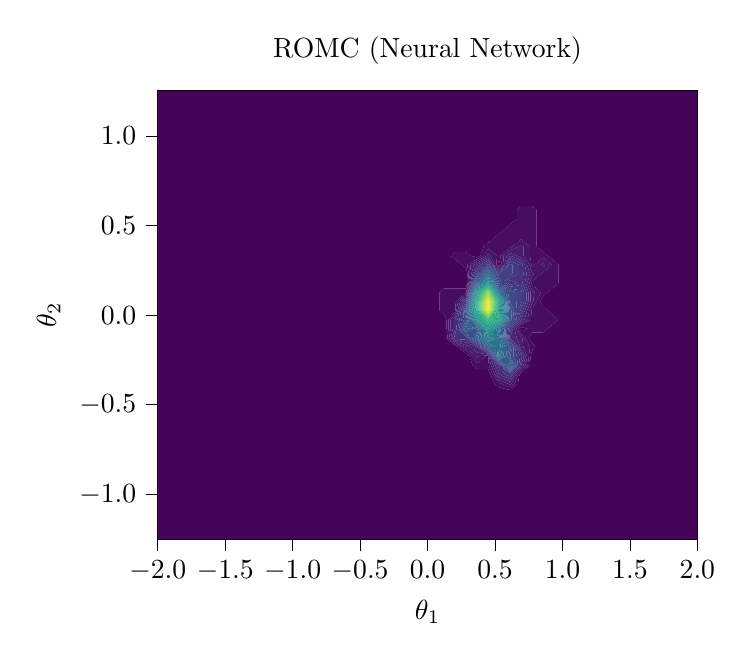
\begin{tikzpicture}

\definecolor{color0}{rgb}{0.269944,0.014625,0.341379}
\definecolor{color1}{rgb}{0.277018,0.050344,0.375715}
\definecolor{color2}{rgb}{0.281446,0.08432,0.407414}
\definecolor{color3}{rgb}{0.283197,0.11568,0.436115}
\definecolor{color4}{rgb}{0.28229,0.145912,0.46151}
\definecolor{color5}{rgb}{0.278826,0.17549,0.483397}
\definecolor{color6}{rgb}{0.274128,0.199721,0.498911}
\definecolor{color7}{rgb}{0.26658,0.228262,0.514349}
\definecolor{color8}{rgb}{0.257322,0.25613,0.526563}
\definecolor{color9}{rgb}{0.246811,0.283237,0.535941}
\definecolor{color10}{rgb}{0.235526,0.309527,0.542944}
\definecolor{color11}{rgb}{0.225863,0.330805,0.547314}
\definecolor{color12}{rgb}{0.214298,0.355619,0.551184}
\definecolor{color13}{rgb}{0.203063,0.379716,0.553925}
\definecolor{color14}{rgb}{0.192357,0.403199,0.555836}
\definecolor{color15}{rgb}{0.182256,0.426184,0.55712}
\definecolor{color16}{rgb}{0.172719,0.448791,0.557885}
\definecolor{color17}{rgb}{0.165117,0.467423,0.558141}
\definecolor{color18}{rgb}{0.15627,0.489624,0.557936}
\definecolor{color19}{rgb}{0.147607,0.511733,0.557049}
\definecolor{color20}{rgb}{0.139147,0.533812,0.555298}
\definecolor{color21}{rgb}{0.131172,0.555899,0.552459}
\definecolor{color22}{rgb}{0.125394,0.574318,0.549086}
\definecolor{color23}{rgb}{0.120565,0.596422,0.543611}
\definecolor{color24}{rgb}{0.119699,0.61849,0.536347}
\definecolor{color25}{rgb}{0.12478,0.640461,0.527068}
\definecolor{color26}{rgb}{0.137339,0.662252,0.515571}
\definecolor{color27}{rgb}{0.157851,0.683765,0.501686}
\definecolor{color28}{rgb}{0.180653,0.701402,0.488189}
\definecolor{color29}{rgb}{0.214,0.722114,0.469588}
\definecolor{color30}{rgb}{0.252899,0.742211,0.448284}
\definecolor{color31}{rgb}{0.296479,0.761561,0.424223}
\definecolor{color32}{rgb}{0.344074,0.780029,0.397381}
\definecolor{color33}{rgb}{0.386433,0.794644,0.372886}
\definecolor{color34}{rgb}{0.440137,0.811138,0.340967}
\definecolor{color35}{rgb}{0.496615,0.826376,0.306377}
\definecolor{color36}{rgb}{0.555484,0.840254,0.269281}
\definecolor{color37}{rgb}{0.616293,0.852709,0.230052}
\definecolor{color38}{rgb}{0.668054,0.861999,0.196293}
\definecolor{color39}{rgb}{0.730889,0.871916,0.156029}
\definecolor{color40}{rgb}{0.79376,0.880678,0.120005}
\definecolor{color41}{rgb}{0.85581,0.888601,0.097452}
\definecolor{color42}{rgb}{0.916242,0.896091,0.100717}
\definecolor{color43}{rgb}{0.974417,0.90359,0.130215}

\begin{axis}[
tick align=outside,
tick pos=left,
title={ROMC (Neural Network)},
x grid style={white!69.0196078431373!black},
xlabel={\(\displaystyle \theta_1\)},
xmin=-2, xmax=2,
xtick style={color=black},
xtick={-2,-1.5,-1,-0.5,0,0.5,1,1.5,2},
xticklabels={
  \(\displaystyle {\ensuremath{-}2.0}\),
  \(\displaystyle {\ensuremath{-}1.5}\),
  \(\displaystyle {\ensuremath{-}1.0}\),
  \(\displaystyle {\ensuremath{-}0.5}\),
  \(\displaystyle {0.0}\),
  \(\displaystyle {0.5}\),
  \(\displaystyle {1.0}\),
  \(\displaystyle {1.5}\),
  \(\displaystyle {2.0}\)
},
y grid style={white!69.0196078431373!black},
ylabel={\(\displaystyle \theta_2\)},
ymin=-1.25, ymax=1.25,
ytick style={color=black},
ytick={-1.5,-1,-0.5,0,0.5,1,1.5},
yticklabels={
  \(\displaystyle {\ensuremath{-}1.5}\),
  \(\displaystyle {\ensuremath{-}1.0}\),
  \(\displaystyle {\ensuremath{-}0.5}\),
  \(\displaystyle {0.0}\),
  \(\displaystyle {0.5}\),
  \(\displaystyle {1.0}\),
  \(\displaystyle {1.5}\)
}
]
\addplot [draw=none, fill=color0]
table{%
x  y
-1.91836734693878 -1.25
-1.83673469387755 -1.25
-1.75510204081633 -1.25
-1.6734693877551 -1.25
-1.59183673469388 -1.25
-1.51020408163265 -1.25
-1.42857142857143 -1.25
-1.3469387755102 -1.25
-1.26530612244898 -1.25
-1.18367346938776 -1.25
-1.10204081632653 -1.25
-1.02040816326531 -1.25
-0.938775510204082 -1.25
-0.857142857142857 -1.25
-0.775510204081633 -1.25
-0.693877551020408 -1.25
-0.612244897959184 -1.25
-0.530612244897959 -1.25
-0.448979591836735 -1.25
-0.36734693877551 -1.25
-0.285714285714286 -1.25
-0.204081632653061 -1.25
-0.122448979591837 -1.25
-0.0408163265306123 -1.25
0.0408163265306123 -1.25
0.122448979591836 -1.25
0.204081632653061 -1.25
0.285714285714286 -1.25
0.36734693877551 -1.25
0.448979591836734 -1.25
0.530612244897959 -1.25
0.612244897959183 -1.25
0.693877551020408 -1.25
0.775510204081633 -1.25
0.857142857142857 -1.25
0.938775510204081 -1.25
1.02040816326531 -1.25
1.10204081632653 -1.25
1.18367346938775 -1.25
1.26530612244898 -1.25
1.3469387755102 -1.25
1.42857142857143 -1.25
1.51020408163265 -1.25
1.59183673469388 -1.25
1.6734693877551 -1.25
1.75510204081633 -1.25
1.83673469387755 -1.25
1.91836734693878 -1.25
2 -1.25
2 -1.19897959183673
2 -1.14795918367347
2 -1.0969387755102
2 -1.04591836734694
2 -0.994897959183674
2 -0.943877551020408
2 -0.892857142857143
2 -0.841836734693878
2 -0.790816326530612
2 -0.739795918367347
2 -0.688775510204082
2 -0.637755102040816
2 -0.586734693877551
2 -0.535714285714286
2 -0.48469387755102
2 -0.433673469387755
2 -0.38265306122449
2 -0.331632653061224
2 -0.280612244897959
2 -0.229591836734694
2 -0.178571428571429
2 -0.127551020408163
2 -0.0765306122448979
2 -0.0255102040816326
2 0.0255102040816326
2 0.0765306122448979
2 0.127551020408163
2 0.178571428571429
2 0.229591836734694
2 0.280612244897959
2 0.331632653061225
2 0.38265306122449
2 0.433673469387755
2 0.48469387755102
2 0.535714285714286
2 0.586734693877551
2 0.637755102040816
2 0.688775510204082
2 0.739795918367347
2 0.790816326530612
2 0.841836734693878
2 0.892857142857143
2 0.943877551020408
2 0.994897959183674
2 1.04591836734694
2 1.0969387755102
2 1.14795918367347
2 1.19897959183673
2 1.25
1.91836734693878 1.25
1.83673469387755 1.25
1.75510204081633 1.25
1.6734693877551 1.25
1.59183673469388 1.25
1.51020408163265 1.25
1.42857142857143 1.25
1.3469387755102 1.25
1.26530612244898 1.25
1.18367346938775 1.25
1.10204081632653 1.25
1.02040816326531 1.25
0.938775510204081 1.25
0.857142857142857 1.25
0.775510204081633 1.25
0.693877551020408 1.25
0.612244897959183 1.25
0.530612244897959 1.25
0.448979591836734 1.25
0.36734693877551 1.25
0.285714285714286 1.25
0.204081632653061 1.25
0.122448979591836 1.25
0.0408163265306123 1.25
-0.0408163265306123 1.25
-0.122448979591837 1.25
-0.204081632653061 1.25
-0.285714285714286 1.25
-0.36734693877551 1.25
-0.448979591836735 1.25
-0.530612244897959 1.25
-0.612244897959184 1.25
-0.693877551020408 1.25
-0.775510204081633 1.25
-0.857142857142857 1.25
-0.938775510204082 1.25
-1.02040816326531 1.25
-1.10204081632653 1.25
-1.18367346938776 1.25
-1.26530612244898 1.25
-1.3469387755102 1.25
-1.42857142857143 1.25
-1.51020408163265 1.25
-1.59183673469388 1.25
-1.6734693877551 1.25
-1.75510204081633 1.25
-1.83673469387755 1.25
-1.91836734693878 1.25
-2 1.25
-2 1.19897959183673
-2 1.14795918367347
-2 1.0969387755102
-2 1.04591836734694
-2 0.994897959183674
-2 0.943877551020408
-2 0.892857142857143
-2 0.841836734693878
-2 0.790816326530612
-2 0.739795918367347
-2 0.688775510204082
-2 0.637755102040816
-2 0.586734693877551
-2 0.535714285714286
-2 0.48469387755102
-2 0.433673469387755
-2 0.38265306122449
-2 0.331632653061225
-2 0.280612244897959
-2 0.229591836734694
-2 0.178571428571429
-2 0.127551020408163
-2 0.0765306122448979
-2 0.0255102040816326
-2 -0.0255102040816326
-2 -0.0765306122448979
-2 -0.127551020408163
-2 -0.178571428571429
-2 -0.229591836734694
-2 -0.280612244897959
-2 -0.331632653061224
-2 -0.38265306122449
-2 -0.433673469387755
-2 -0.48469387755102
-2 -0.535714285714286
-2 -0.586734693877551
-2 -0.637755102040816
-2 -0.688775510204082
-2 -0.739795918367347
-2 -0.790816326530612
-2 -0.841836734693878
-2 -0.892857142857143
-2 -0.943877551020408
-2 -0.994897959183674
-2 -1.04591836734694
-2 -1.0969387755102
-2 -1.14795918367347
-2 -1.19897959183673
-2 -1.25
-1.91836734693878 -1.25

0.497959183673469 -0.38265306122449
0.465306122448979 -0.331632653061224
0.448979591836734 -0.301020408163265
0.36734693877551 -0.301020408163265
0.33469387755102 -0.280612244897959
0.310204081632653 -0.229591836734694
0.285714285714286 -0.214285714285714
0.228571428571428 -0.178571428571429
0.204081632653061 -0.170918367346939
0.13469387755102 -0.127551020408163
0.138775510204081 -0.0765306122448979
0.138775510204081 -0.0255102040816326
0.122448979591836 0.00510204081632653
0.0897959183673468 0.0255102040816326
0.0897959183673468 0.0765306122448979
0.0897959183673468 0.127551020408163
0.122448979591836 0.147959183673469
0.204081632653061 0.147959183673469
0.285714285714286 0.147959183673469
0.291836734693877 0.178571428571429
0.295510204081633 0.229591836734694
0.285714285714286 0.260204081632653
0.253061224489796 0.280612244897959
0.204081632653061 0.311224489795918
0.171428571428571 0.331632653061225
0.204081632653061 0.352040816326531
0.285714285714286 0.352040816326531
0.318367346938775 0.331632653061225
0.36734693877551 0.321428571428572
0.391836734693877 0.331632653061225
0.416326530612245 0.38265306122449
0.448979591836734 0.403061224489796
0.497959183673469 0.433673469387755
0.530612244897959 0.454081632653061
0.579591836734694 0.48469387755102
0.612244897959183 0.505102040816326
0.661224489795918 0.535714285714286
0.661224489795918 0.586734693877551
0.693877551020408 0.607142857142857
0.775510204081633 0.607142857142857
0.808163265306122 0.586734693877551
0.808163265306122 0.535714285714286
0.808163265306122 0.48469387755102
0.808163265306122 0.433673469387755
0.808163265306122 0.38265306122449
0.857142857142857 0.352040816326531
0.889795918367347 0.331632653061225
0.938775510204081 0.301020408163265
0.971428571428571 0.280612244897959
0.971428571428571 0.229591836734694
0.971428571428571 0.178571428571429
0.938775510204081 0.158163265306123
0.889795918367347 0.127551020408163
0.857142857142857 0.107142857142857
0.832653061224489 0.0765306122448979
0.857142857142857 0.0459183673469387
0.889795918367347 0.0255102040816326
0.938775510204081 -0.00510204081632653
0.971428571428571 -0.0255102040816326
0.938775510204081 -0.0459183673469387
0.889795918367347 -0.0765306122448979
0.857142857142857 -0.096938775510204
0.775510204081633 -0.096938775510204
0.751020408163265 -0.127551020408163
0.775510204081633 -0.158163265306122
0.808163265306122 -0.178571428571429
0.775510204081633 -0.198979591836735
0.763265306122449 -0.229591836734694
0.759183673469388 -0.280612244897959
0.693877551020408 -0.321428571428571
0.681632653061224 -0.331632653061224
0.669387755102041 -0.38265306122449
0.612244897959183 -0.418367346938776
0.530612244897959 -0.403061224489796
0.497959183673469 -0.38265306122449
};
\addplot [draw=none, fill=color0]
table{%
x  y
0.693877551020408 -0.0918367346938775
0.742857142857143 -0.0765306122448979
0.693877551020408 -0.0663265306122448
0.681632653061224 -0.0765306122448979
0.693877551020408 -0.0918367346938775
};
\addplot [draw=none, fill=color0]
table{%
x  y
0.530612244897959 0.274489795918367
0.540408163265306 0.280612244897959
0.530612244897959 0.311224489795918
0.520816326530612 0.280612244897959
0.530612244897959 0.274489795918367
};
\addplot [draw=none, fill=color1]
table{%
x  y
0.530612244897959 -0.403061224489796
0.612244897959183 -0.418367346938776
0.669387755102041 -0.38265306122449
0.681632653061224 -0.331632653061224
0.693877551020408 -0.321428571428571
0.759183673469388 -0.280612244897959
0.763265306122449 -0.229591836734694
0.775510204081633 -0.198979591836735
0.808163265306122 -0.178571428571429
0.775510204081633 -0.158163265306122
0.751020408163265 -0.127551020408163
0.775510204081633 -0.096938775510204
0.857142857142857 -0.096938775510204
0.889795918367347 -0.0765306122448979
0.938775510204081 -0.0459183673469387
0.971428571428571 -0.0255102040816326
0.938775510204081 -0.00510204081632653
0.889795918367347 0.0255102040816326
0.857142857142857 0.0459183673469387
0.832653061224489 0.0765306122448979
0.857142857142857 0.107142857142857
0.889795918367347 0.127551020408163
0.938775510204081 0.158163265306123
0.971428571428571 0.178571428571429
0.971428571428571 0.229591836734694
0.971428571428571 0.280612244897959
0.938775510204081 0.301020408163265
0.889795918367347 0.331632653061225
0.857142857142857 0.352040816326531
0.808163265306122 0.38265306122449
0.808163265306122 0.433673469387755
0.808163265306122 0.48469387755102
0.808163265306122 0.535714285714286
0.808163265306122 0.586734693877551
0.775510204081633 0.607142857142857
0.693877551020408 0.607142857142857
0.661224489795918 0.586734693877551
0.661224489795918 0.535714285714286
0.612244897959183 0.505102040816326
0.579591836734694 0.48469387755102
0.530612244897959 0.454081632653061
0.497959183673469 0.433673469387755
0.448979591836734 0.403061224489796
0.416326530612245 0.38265306122449
0.391836734693877 0.331632653061225
0.36734693877551 0.321428571428572
0.318367346938775 0.331632653061225
0.285714285714286 0.352040816326531
0.204081632653061 0.352040816326531
0.171428571428571 0.331632653061225
0.204081632653061 0.311224489795918
0.253061224489796 0.280612244897959
0.285714285714286 0.260204081632653
0.295510204081633 0.229591836734694
0.291836734693877 0.178571428571429
0.285714285714286 0.147959183673469
0.204081632653061 0.147959183673469
0.122448979591836 0.147959183673469
0.0897959183673468 0.127551020408163
0.0897959183673468 0.0765306122448979
0.0897959183673468 0.0255102040816326
0.122448979591836 0.00510204081632653
0.138775510204081 -0.0255102040816326
0.138775510204081 -0.0765306122448979
0.13469387755102 -0.127551020408163
0.204081632653061 -0.170918367346939
0.228571428571428 -0.178571428571429
0.285714285714286 -0.214285714285714
0.310204081632653 -0.229591836734694
0.33469387755102 -0.280612244897959
0.36734693877551 -0.301020408163265
0.448979591836734 -0.301020408163265
0.465306122448979 -0.331632653061224
0.497959183673469 -0.38265306122449
0.530612244897959 -0.403061224489796

0.546938775510204 -0.38265306122449
0.530612244897959 -0.377551020408163
0.481632653061224 -0.331632653061224
0.454421768707483 -0.280612244897959
0.450612244897959 -0.229591836734694
0.448979591836734 -0.228134110787172
0.432653061224489 -0.229591836734694
0.36734693877551 -0.270408163265306
0.33469387755102 -0.229591836734694
0.285714285714286 -0.198979591836735
0.253061224489796 -0.178571428571429
0.204081632653061 -0.163265306122449
0.146938775510204 -0.127551020408163
0.155102040816326 -0.0765306122448979
0.155102040816326 -0.0255102040816326
0.204081632653061 0.0204081632653061
0.206802721088435 0.0255102040816326
0.209523809523809 0.0765306122448979
0.285714285714286 0.124149659863946
0.286970172684458 0.127551020408163
0.297959183673469 0.178571428571429
0.305306122448979 0.229591836734694
0.293877551020408 0.280612244897959
0.36734693877551 0.311224489795918
0.416326530612245 0.331632653061225
0.448979591836734 0.372448979591837
0.514285714285714 0.331632653061225
0.511020408163265 0.280612244897959
0.530612244897959 0.268367346938776
0.550204081632653 0.280612244897959
0.538775510204081 0.331632653061225
0.612244897959183 0.377551020408163
0.628571428571428 0.38265306122449
0.693877551020408 0.423469387755102
0.759183673469388 0.38265306122449
0.759183673469388 0.331632653061225
0.770068027210884 0.280612244897959
0.775510204081633 0.270408163265306
0.791836734693877 0.280612244897959
0.857142857142857 0.321428571428572
0.922448979591836 0.280612244897959
0.857142857142857 0.239795918367347
0.840816326530612 0.229591836734694
0.775510204081633 0.188775510204082
0.770068027210884 0.178571428571429
0.775510204081633 0.168367346938776
0.840816326530612 0.127551020408163
0.808163265306122 0.0765306122448979
0.775510204081633 0.0357142857142857
0.770068027210884 0.0255102040816326
0.76734693877551 -0.0255102040816326
0.693877551020408 -0.0561224489795918
0.669387755102041 -0.0765306122448979
0.693877551020408 -0.107142857142857
0.726530612244898 -0.127551020408163
0.759183673469388 -0.178571428571429
0.751020408163265 -0.229591836734694
0.742857142857143 -0.280612244897959
0.693877551020408 -0.311224489795918
0.669387755102041 -0.331632653061224
0.644897959183673 -0.38265306122449
0.612244897959183 -0.403061224489796
0.546938775510204 -0.38265306122449

0.681632653061224 -0.0765306122448979
0.693877551020408 -0.0663265306122448
0.742857142857143 -0.0765306122448979
0.693877551020408 -0.0918367346938775
0.681632653061224 -0.0765306122448979

0.520816326530612 0.280612244897959
0.530612244897959 0.311224489795918
0.540408163265306 0.280612244897959
0.530612244897959 0.274489795918367
0.520816326530612 0.280612244897959
};
\addplot [draw=none, fill=color2]
table{%
x  y
0.612244897959183 -0.403061224489796
0.644897959183673 -0.38265306122449
0.669387755102041 -0.331632653061224
0.693877551020408 -0.311224489795918
0.742857142857143 -0.280612244897959
0.751020408163265 -0.229591836734694
0.759183673469388 -0.178571428571429
0.726530612244898 -0.127551020408163
0.693877551020408 -0.107142857142857
0.669387755102041 -0.0765306122448979
0.693877551020408 -0.0561224489795918
0.76734693877551 -0.0255102040816326
0.770068027210884 0.0255102040816326
0.775510204081633 0.0357142857142857
0.808163265306122 0.0765306122448979
0.840816326530612 0.127551020408163
0.775510204081633 0.168367346938776
0.770068027210884 0.178571428571429
0.775510204081633 0.188775510204082
0.840816326530612 0.229591836734694
0.857142857142857 0.239795918367347
0.922448979591836 0.280612244897959
0.857142857142857 0.321428571428572
0.791836734693877 0.280612244897959
0.775510204081633 0.270408163265306
0.770068027210884 0.280612244897959
0.759183673469388 0.331632653061225
0.759183673469388 0.38265306122449
0.693877551020408 0.423469387755102
0.628571428571428 0.38265306122449
0.612244897959183 0.377551020408163
0.538775510204081 0.331632653061225
0.550204081632653 0.280612244897959
0.530612244897959 0.268367346938776
0.511020408163265 0.280612244897959
0.514285714285714 0.331632653061225
0.448979591836734 0.372448979591837
0.416326530612245 0.331632653061225
0.36734693877551 0.311224489795918
0.293877551020408 0.280612244897959
0.305306122448979 0.229591836734694
0.297959183673469 0.178571428571429
0.286970172684458 0.127551020408163
0.285714285714286 0.124149659863946
0.209523809523809 0.0765306122448979
0.206802721088435 0.0255102040816326
0.204081632653061 0.0204081632653061
0.155102040816326 -0.0255102040816326
0.155102040816326 -0.0765306122448979
0.146938775510204 -0.127551020408163
0.204081632653061 -0.163265306122449
0.253061224489796 -0.178571428571429
0.285714285714286 -0.198979591836735
0.33469387755102 -0.229591836734694
0.36734693877551 -0.270408163265306
0.432653061224489 -0.229591836734694
0.448979591836734 -0.228134110787172
0.450612244897959 -0.229591836734694
0.454421768707483 -0.280612244897959
0.481632653061224 -0.331632653061224
0.530612244897959 -0.377551020408163
0.546938775510204 -0.38265306122449
0.612244897959183 -0.403061224489796

0.595918367346939 -0.38265306122449
0.530612244897959 -0.362244897959184
0.497959183673469 -0.331632653061224
0.470748299319728 -0.280612244897959
0.455510204081632 -0.229591836734694
0.448979591836734 -0.223760932944606
0.383673469387755 -0.229591836734694
0.36734693877551 -0.239795918367347
0.359183673469388 -0.229591836734694
0.285714285714286 -0.183673469387755
0.277551020408163 -0.178571428571429
0.204081632653061 -0.155612244897959
0.159183673469387 -0.127551020408163
0.171428571428571 -0.0765306122448979
0.171428571428571 -0.0255102040816326
0.204081632653061 0.00510204081632652
0.214965986394558 0.0255102040816326
0.225850340136054 0.0765306122448979
0.285714285714286 0.113945578231293
0.290737833594976 0.127551020408163
0.304081632653061 0.178571428571429
0.315102040816326 0.229591836734694
0.318367346938775 0.280612244897959
0.36734693877551 0.301020408163265
0.440816326530612 0.331632653061225
0.448979591836734 0.341836734693878
0.465306122448979 0.331632653061225
0.501224489795918 0.280612244897959
0.530612244897959 0.262244897959184
0.56 0.280612244897959
0.563265306122449 0.331632653061225
0.612244897959183 0.362244897959184
0.677551020408163 0.38265306122449
0.693877551020408 0.392857142857143
0.710204081632653 0.38265306122449
0.710204081632653 0.331632653061225
0.753741496598639 0.280612244897959
0.775510204081633 0.239795918367347
0.791836734693877 0.229591836734694
0.775510204081633 0.219387755102041
0.753741496598639 0.178571428571429
0.775510204081633 0.137755102040816
0.791836734693877 0.127551020408163
0.783673469387755 0.0765306122448979
0.775510204081633 0.0663265306122448
0.753741496598639 0.0255102040816326
0.742857142857143 -0.0255102040816326
0.693877551020408 -0.0459183673469387
0.657142857142857 -0.0765306122448979
0.693877551020408 -0.122448979591837
0.70204081632653 -0.127551020408163
0.710204081632653 -0.178571428571429
0.738775510204082 -0.229591836734694
0.726530612244898 -0.280612244897959
0.693877551020408 -0.301020408163265
0.657142857142857 -0.331632653061224
0.620408163265306 -0.38265306122449
0.612244897959183 -0.387755102040816
0.595918367346939 -0.38265306122449

0.840816326530612 0.280612244897959
0.857142857142857 0.290816326530612
0.873469387755102 0.280612244897959
0.857142857142857 0.270408163265306
0.840816326530612 0.280612244897959
};
\addplot [draw=none, fill=color3]
table{%
x  y
0.612244897959183 -0.387755102040816
0.620408163265306 -0.38265306122449
0.657142857142857 -0.331632653061224
0.693877551020408 -0.301020408163265
0.726530612244898 -0.280612244897959
0.738775510204082 -0.229591836734694
0.710204081632653 -0.178571428571429
0.70204081632653 -0.127551020408163
0.693877551020408 -0.122448979591837
0.657142857142857 -0.0765306122448979
0.693877551020408 -0.0459183673469387
0.742857142857143 -0.0255102040816326
0.753741496598639 0.0255102040816326
0.775510204081633 0.0663265306122448
0.783673469387755 0.0765306122448979
0.791836734693877 0.127551020408163
0.775510204081633 0.137755102040816
0.753741496598639 0.178571428571429
0.775510204081633 0.219387755102041
0.791836734693877 0.229591836734694
0.775510204081633 0.239795918367347
0.753741496598639 0.280612244897959
0.710204081632653 0.331632653061225
0.710204081632653 0.38265306122449
0.693877551020408 0.392857142857143
0.677551020408163 0.38265306122449
0.612244897959183 0.362244897959184
0.563265306122449 0.331632653061225
0.56 0.280612244897959
0.530612244897959 0.262244897959184
0.501224489795918 0.280612244897959
0.465306122448979 0.331632653061225
0.448979591836734 0.341836734693878
0.440816326530612 0.331632653061225
0.36734693877551 0.301020408163265
0.318367346938775 0.280612244897959
0.315102040816326 0.229591836734694
0.304081632653061 0.178571428571429
0.290737833594976 0.127551020408163
0.285714285714286 0.113945578231293
0.225850340136054 0.0765306122448979
0.214965986394558 0.0255102040816326
0.204081632653061 0.00510204081632652
0.171428571428571 -0.0255102040816326
0.171428571428571 -0.0765306122448979
0.159183673469387 -0.127551020408163
0.204081632653061 -0.155612244897959
0.277551020408163 -0.178571428571429
0.285714285714286 -0.183673469387755
0.359183673469388 -0.229591836734694
0.36734693877551 -0.239795918367347
0.383673469387755 -0.229591836734694
0.448979591836734 -0.223760932944606
0.455510204081632 -0.229591836734694
0.470748299319728 -0.280612244897959
0.497959183673469 -0.331632653061224
0.530612244897959 -0.362244897959184
0.595918367346939 -0.38265306122449
0.612244897959183 -0.387755102040816

0.514285714285714 -0.331632653061224
0.487074829931972 -0.280612244897959
0.460408163265306 -0.229591836734694
0.448979591836734 -0.219387755102041
0.36734693877551 -0.209183673469388
0.318367346938775 -0.178571428571429
0.285714285714286 -0.168367346938776
0.204081632653061 -0.147959183673469
0.171428571428571 -0.127551020408163
0.187755102040816 -0.0765306122448979
0.187755102040816 -0.0255102040816326
0.204081632653061 -0.0102040816326531
0.22312925170068 0.0255102040816326
0.242176870748299 0.0765306122448979
0.285714285714286 0.103741496598639
0.294505494505494 0.127551020408163
0.310204081632653 0.178571428571429
0.324897959183673 0.229591836734694
0.342857142857143 0.280612244897959
0.36734693877551 0.290816326530612
0.448979591836734 0.324829931972789
0.491428571428571 0.280612244897959
0.530612244897959 0.256122448979592
0.569795918367347 0.280612244897959
0.587755102040816 0.331632653061225
0.612244897959183 0.346938775510204
0.661224489795918 0.331632653061225
0.693877551020408 0.321428571428572
0.737414965986394 0.280612244897959
0.759183673469388 0.229591836734694
0.737414965986394 0.178571428571429
0.764625850340136 0.127551020408163
0.764625850340136 0.0765306122448979
0.737414965986394 0.0255102040816326
0.718367346938775 -0.0255102040816326
0.693877551020408 -0.0357142857142857
0.644897959183673 -0.0765306122448979
0.661224489795918 -0.127551020408163
0.68734693877551 -0.178571428571429
0.693877551020408 -0.188775510204082
0.726530612244898 -0.229591836734694
0.710204081632653 -0.280612244897959
0.693877551020408 -0.290816326530612
0.644897959183673 -0.331632653061224
0.612244897959183 -0.372448979591837
0.530612244897959 -0.346938775510204
0.514285714285714 -0.331632653061224
};
\addplot [draw=none, fill=color3]
table{%
x  y
0.857142857142857 0.270408163265306
0.873469387755102 0.280612244897959
0.857142857142857 0.290816326530612
0.840816326530612 0.280612244897959
0.857142857142857 0.270408163265306
};
\addplot [draw=none, fill=color4]
table{%
x  y
0.530612244897959 -0.346938775510204
0.612244897959183 -0.372448979591837
0.644897959183673 -0.331632653061224
0.693877551020408 -0.290816326530612
0.710204081632653 -0.280612244897959
0.726530612244898 -0.229591836734694
0.693877551020408 -0.188775510204082
0.68734693877551 -0.178571428571429
0.661224489795918 -0.127551020408163
0.644897959183673 -0.0765306122448979
0.693877551020408 -0.0357142857142857
0.718367346938775 -0.0255102040816326
0.737414965986394 0.0255102040816326
0.764625850340136 0.0765306122448979
0.764625850340136 0.127551020408163
0.737414965986394 0.178571428571429
0.759183673469388 0.229591836734694
0.737414965986394 0.280612244897959
0.693877551020408 0.321428571428572
0.661224489795918 0.331632653061225
0.612244897959183 0.346938775510204
0.587755102040816 0.331632653061225
0.569795918367347 0.280612244897959
0.530612244897959 0.256122448979592
0.491428571428571 0.280612244897959
0.448979591836734 0.324829931972789
0.36734693877551 0.290816326530612
0.342857142857143 0.280612244897959
0.324897959183673 0.229591836734694
0.310204081632653 0.178571428571429
0.294505494505494 0.127551020408163
0.285714285714286 0.103741496598639
0.242176870748299 0.0765306122448979
0.22312925170068 0.0255102040816326
0.204081632653061 -0.0102040816326531
0.187755102040816 -0.0255102040816326
0.187755102040816 -0.0765306122448979
0.171428571428571 -0.127551020408163
0.204081632653061 -0.147959183673469
0.285714285714286 -0.168367346938776
0.318367346938775 -0.178571428571429
0.36734693877551 -0.209183673469388
0.448979591836734 -0.219387755102041
0.460408163265306 -0.229591836734694
0.487074829931972 -0.280612244897959
0.514285714285714 -0.331632653061224
0.530612244897959 -0.346938775510204

0.530612244897959 -0.331632653061224
0.530612244897959 -0.331632653061224
0.503401360544217 -0.280612244897959
0.465306122448979 -0.229591836734694
0.448979591836734 -0.215014577259475
0.36734693877551 -0.178571428571429
0.285714285714286 -0.153061224489796
0.204081632653061 -0.140306122448979
0.183673469387755 -0.127551020408163
0.204081632653061 -0.0765306122448979
0.204081632653061 -0.0765306122448979
0.204081632653061 -0.0255102040816326
0.231292517006803 0.0255102040816326
0.258503401360544 0.0765306122448979
0.285714285714286 0.0935374149659864
0.298273155416012 0.127551020408163
0.316326530612245 0.178571428571429
0.33469387755102 0.229591836734694
0.36734693877551 0.280612244897959
0.36734693877551 0.280612244897959
0.448979591836734 0.314625850340136
0.481632653061224 0.280612244897959
0.530612244897959 0.25
0.579591836734694 0.280612244897959
0.612244897959183 0.331632653061225
0.693877551020408 0.306122448979592
0.72108843537415 0.280612244897959
0.73469387755102 0.229591836734694
0.72108843537415 0.178571428571429
0.748299319727891 0.127551020408163
0.748299319727891 0.0765306122448979
0.72108843537415 0.0255102040816326
0.693877551020408 -0.0255102040816326
0.693877551020408 -0.0255102040816326
0.63265306122449 -0.0765306122448979
0.612244897959183 -0.127551020408163
0.612244897959183 -0.127551020408163
0.612244897959183 -0.127551020408163
0.677551020408163 -0.178571428571429
0.693877551020408 -0.204081632653061
0.714285714285714 -0.229591836734694
0.693877551020408 -0.280612244897959
0.693877551020408 -0.280612244897959
0.63265306122449 -0.331632653061224
0.612244897959183 -0.357142857142857
0.530612244897959 -0.331632653061224
};
\addplot [draw=none, fill=color4]
table{%
x  y
0.612244897959183 0.178571428571429
0.612244897959184 0.178571428571429
0.612244897959183 0.178571428571429
0.612244897959183 0.178571428571429
0.612244897959183 0.178571428571429
};
\addplot [draw=none, fill=color5]
table{%
x  y
0.612244897959183 -0.357142857142857
0.63265306122449 -0.331632653061224
0.693877551020408 -0.280612244897959
0.714285714285714 -0.229591836734694
0.693877551020408 -0.204081632653061
0.677551020408163 -0.178571428571429
0.612244897959183 -0.127551020408163
0.612244897959183 -0.127551020408163
0.63265306122449 -0.0765306122448979
0.693877551020408 -0.0255102040816326
0.693877551020408 -0.0255102040816326
0.72108843537415 0.0255102040816326
0.748299319727891 0.0765306122448979
0.748299319727891 0.127551020408163
0.72108843537415 0.178571428571429
0.73469387755102 0.229591836734694
0.72108843537415 0.280612244897959
0.693877551020408 0.306122448979592
0.612244897959183 0.331632653061225
0.579591836734694 0.280612244897959
0.530612244897959 0.25
0.481632653061224 0.280612244897959
0.448979591836734 0.314625850340136
0.36734693877551 0.280612244897959
0.36734693877551 0.280612244897959
0.33469387755102 0.229591836734694
0.316326530612245 0.178571428571429
0.298273155416012 0.127551020408163
0.285714285714286 0.0935374149659864
0.258503401360544 0.0765306122448979
0.231292517006803 0.0255102040816326
0.204081632653061 -0.0255102040816326
0.204081632653061 -0.0765306122448979
0.204081632653061 -0.0765306122448979
0.183673469387755 -0.127551020408163
0.204081632653061 -0.140306122448979
0.285714285714286 -0.153061224489796
0.36734693877551 -0.178571428571429
0.36734693877551 -0.178571428571429
0.448979591836734 -0.215014577259475
0.465306122448979 -0.229591836734694
0.503401360544217 -0.280612244897959
0.530612244897959 -0.331632653061224
0.530612244897959 -0.331632653061224
0.612244897959183 -0.357142857142857

0.579591836734694 -0.331632653061224
0.530612244897959 -0.301020408163265
0.519727891156462 -0.280612244897959
0.470204081632653 -0.229591836734694
0.448979591836734 -0.21064139941691
0.377142857142857 -0.178571428571429
0.36734693877551 -0.172448979591837
0.285714285714286 -0.137755102040816
0.204081632653061 -0.13265306122449
0.195918367346939 -0.127551020408163
0.204081632653061 -0.107142857142857
0.213877551020408 -0.0765306122448979
0.220408163265306 -0.0255102040816326
0.239455782312925 0.0255102040816326
0.274829931972789 0.0765306122448979
0.285714285714286 0.0833333333333333
0.302040816326531 0.127551020408163
0.322448979591837 0.178571428571429
0.344489795918367 0.229591836734694
0.36734693877551 0.26530612244898
0.391836734693877 0.280612244897959
0.448979591836734 0.304421768707483
0.471836734693877 0.280612244897959
0.530612244897959 0.243877551020408
0.589387755102041 0.280612244897959
0.612244897959183 0.316326530612245
0.693877551020408 0.290816326530612
0.704761904761905 0.280612244897959
0.710204081632653 0.229591836734694
0.704761904761905 0.178571428571429
0.731972789115646 0.127551020408163
0.731972789115646 0.0765306122448979
0.704761904761905 0.0255102040816326
0.693877551020408 0.00510204081632655
0.681632653061224 -0.0255102040816326
0.620408163265306 -0.0765306122448979
0.612244897959183 -0.0969387755102039
0.605247813411079 -0.127551020408163
0.612244897959183 -0.135204081632653
0.667755102040816 -0.178571428571429
0.693877551020408 -0.219387755102041
0.70204081632653 -0.229591836734694
0.693877551020408 -0.25
0.685714285714286 -0.280612244897959
0.620408163265306 -0.331632653061224
0.612244897959183 -0.341836734693878
0.579591836734694 -0.331632653061224
};
\addplot [draw=none, fill=color5]
table{%
x  y
0.612244897959183 0.168367346938776
0.661224489795918 0.178571428571429
0.612244897959183 0.193877551020408
0.595918367346938 0.178571428571429
0.612244897959183 0.168367346938776

0.612244897959183 0.178571428571429
0.612244897959183 0.178571428571429
0.612244897959184 0.178571428571429
0.612244897959183 0.178571428571429
0.612244897959183 0.178571428571429
};
\addplot [draw=none, fill=color6]
table{%
x  y
0.612244897959183 -0.341836734693878
0.620408163265306 -0.331632653061224
0.685714285714286 -0.280612244897959
0.693877551020408 -0.25
0.70204081632653 -0.229591836734694
0.693877551020408 -0.219387755102041
0.667755102040816 -0.178571428571429
0.612244897959183 -0.135204081632653
0.605247813411078 -0.127551020408163
0.612244897959183 -0.0969387755102039
0.620408163265306 -0.0765306122448979
0.681632653061224 -0.0255102040816326
0.693877551020408 0.00510204081632655
0.704761904761905 0.0255102040816326
0.731972789115646 0.0765306122448979
0.731972789115646 0.127551020408163
0.704761904761905 0.178571428571429
0.710204081632653 0.229591836734694
0.704761904761905 0.280612244897959
0.693877551020408 0.290816326530612
0.612244897959183 0.316326530612245
0.589387755102041 0.280612244897959
0.530612244897959 0.243877551020408
0.471836734693877 0.280612244897959
0.448979591836734 0.304421768707483
0.391836734693877 0.280612244897959
0.36734693877551 0.26530612244898
0.344489795918367 0.229591836734694
0.322448979591837 0.178571428571429
0.302040816326531 0.127551020408163
0.285714285714286 0.0833333333333333
0.274829931972789 0.0765306122448979
0.239455782312925 0.0255102040816326
0.220408163265306 -0.0255102040816326
0.213877551020408 -0.0765306122448979
0.204081632653061 -0.107142857142857
0.195918367346939 -0.127551020408163
0.204081632653061 -0.13265306122449
0.285714285714286 -0.137755102040816
0.36734693877551 -0.172448979591837
0.377142857142857 -0.178571428571429
0.448979591836734 -0.21064139941691
0.470204081632653 -0.229591836734694
0.519727891156462 -0.280612244897959
0.530612244897959 -0.301020408163265
0.579591836734694 -0.331632653061224
0.612244897959183 -0.341836734693878

0.533877551020408 -0.280612244897959
0.530612244897959 -0.279154518950437
0.475102040816326 -0.229591836734694
0.448979591836734 -0.206268221574344
0.386938775510204 -0.178571428571429
0.36734693877551 -0.166326530612245
0.289795918367347 -0.127551020408163
0.285714285714286 -0.125
0.223673469387755 -0.0765306122448979
0.236734693877551 -0.0255102040816326
0.247619047619047 0.0255102040816326
0.285714285714286 0.0731292517006802
0.287074829931973 0.0765306122448979
0.305808477237049 0.127551020408163
0.328571428571429 0.178571428571429
0.354285714285714 0.229591836734694
0.36734693877551 0.25
0.416326530612245 0.280612244897959
0.448979591836734 0.29421768707483
0.46204081632653 0.280612244897959
0.530612244897959 0.237755102040816
0.599183673469388 0.280612244897959
0.612244897959183 0.301020408163265
0.677551020408163 0.280612244897959
0.677551020408163 0.229591836734694
0.612244897959183 0.209183673469388
0.579591836734694 0.178571428571429
0.612244897959183 0.158163265306122
0.693877551020408 0.168367346938775
0.715646258503401 0.127551020408163
0.715646258503401 0.0765306122448979
0.693877551020408 0.0357142857142857
0.68843537414966 0.0255102040816326
0.669387755102041 -0.0255102040816326
0.612244897959183 -0.0731292517006802
0.608979591836734 -0.0765306122448979
0.598250728862973 -0.127551020408163
0.612244897959183 -0.142857142857143
0.657959183673469 -0.178571428571429
0.685714285714285 -0.229591836734694
0.677551020408163 -0.280612244897959
0.612244897959183 -0.329591836734694
0.533877551020408 -0.280612244897959

0.595918367346938 0.178571428571429
0.612244897959183 0.193877551020408
0.661224489795918 0.178571428571429
0.612244897959183 0.168367346938776
0.595918367346938 0.178571428571429
};
\addplot [draw=none, fill=color7]
table{%
x  y
0.612244897959183 -0.329591836734694
0.677551020408163 -0.280612244897959
0.685714285714285 -0.229591836734694
0.657959183673469 -0.178571428571429
0.612244897959183 -0.142857142857143
0.598250728862973 -0.127551020408163
0.608979591836734 -0.0765306122448979
0.612244897959183 -0.0731292517006802
0.669387755102041 -0.0255102040816326
0.68843537414966 0.0255102040816326
0.693877551020408 0.0357142857142857
0.715646258503401 0.0765306122448979
0.715646258503401 0.127551020408163
0.693877551020408 0.168367346938775
0.612244897959183 0.158163265306122
0.579591836734694 0.178571428571429
0.612244897959183 0.209183673469388
0.677551020408163 0.229591836734694
0.677551020408163 0.280612244897959
0.612244897959183 0.301020408163265
0.599183673469388 0.280612244897959
0.530612244897959 0.237755102040816
0.46204081632653 0.280612244897959
0.448979591836734 0.29421768707483
0.416326530612245 0.280612244897959
0.36734693877551 0.25
0.354285714285714 0.229591836734694
0.328571428571429 0.178571428571429
0.305808477237049 0.127551020408163
0.287074829931973 0.0765306122448979
0.285714285714286 0.0731292517006802
0.247619047619047 0.0255102040816326
0.236734693877551 -0.0255102040816326
0.223673469387755 -0.0765306122448979
0.285714285714286 -0.125
0.289795918367347 -0.127551020408163
0.36734693877551 -0.166326530612245
0.386938775510204 -0.178571428571429
0.448979591836734 -0.206268221574344
0.475102040816326 -0.229591836734694
0.530612244897959 -0.279154518950437
0.533877551020408 -0.280612244897959
0.612244897959183 -0.329591836734694

0.543673469387755 -0.280612244897959
0.530612244897959 -0.274781341107872
0.48 -0.229591836734694
0.448979591836734 -0.201895043731778
0.396734693877551 -0.178571428571429
0.36734693877551 -0.160204081632653
0.302040816326531 -0.127551020408163
0.285714285714286 -0.11734693877551
0.233469387755102 -0.0765306122448979
0.253061224489796 -0.0255102040816326
0.25578231292517 0.0255102040816326
0.285714285714286 0.0629251700680271
0.291156462585034 0.0765306122448979
0.309576138147567 0.127551020408163
0.33469387755102 0.178571428571429
0.364081632653061 0.229591836734694
0.36734693877551 0.23469387755102
0.440816326530612 0.280612244897959
0.448979591836734 0.284013605442177
0.452244897959183 0.280612244897959
0.530612244897959 0.231632653061224
0.608979591836735 0.280612244897959
0.612244897959183 0.285714285714286
0.628571428571428 0.280612244897959
0.628571428571428 0.229591836734694
0.612244897959183 0.224489795918367
0.563265306122449 0.178571428571429
0.612244897959183 0.147959183673469
0.693877551020408 0.137755102040816
0.699319727891156 0.127551020408163
0.699319727891156 0.0765306122448979
0.693877551020408 0.0663265306122449
0.672108843537415 0.0255102040816326
0.657142857142857 -0.0255102040816326
0.612244897959183 -0.0629251700680271
0.599183673469388 -0.0765306122448979
0.591253644314869 -0.127551020408163
0.612244897959183 -0.150510204081633
0.648163265306122 -0.178571428571429
0.661224489795918 -0.229591836734694
0.669387755102041 -0.280612244897959
0.612244897959183 -0.323469387755102
0.543673469387755 -0.280612244897959
};
\addplot [draw=none, fill=color8]
table{%
x  y
0.612244897959183 -0.323469387755102
0.669387755102041 -0.280612244897959
0.661224489795918 -0.229591836734694
0.648163265306122 -0.178571428571429
0.612244897959183 -0.150510204081633
0.591253644314869 -0.127551020408163
0.599183673469388 -0.0765306122448979
0.612244897959183 -0.0629251700680271
0.657142857142857 -0.0255102040816326
0.672108843537415 0.0255102040816326
0.693877551020408 0.0663265306122449
0.699319727891156 0.0765306122448979
0.699319727891156 0.127551020408163
0.693877551020408 0.137755102040816
0.612244897959183 0.147959183673469
0.563265306122449 0.178571428571429
0.612244897959183 0.224489795918367
0.628571428571428 0.229591836734694
0.628571428571428 0.280612244897959
0.612244897959183 0.285714285714286
0.608979591836735 0.280612244897959
0.530612244897959 0.231632653061224
0.452244897959183 0.280612244897959
0.448979591836734 0.284013605442177
0.440816326530612 0.280612244897959
0.36734693877551 0.23469387755102
0.364081632653061 0.229591836734694
0.33469387755102 0.178571428571429
0.309576138147567 0.127551020408163
0.291156462585034 0.0765306122448979
0.285714285714286 0.0629251700680271
0.25578231292517 0.0255102040816326
0.253061224489796 -0.0255102040816326
0.233469387755102 -0.0765306122448979
0.285714285714286 -0.11734693877551
0.302040816326531 -0.127551020408163
0.36734693877551 -0.160204081632653
0.396734693877551 -0.178571428571429
0.448979591836734 -0.201895043731778
0.48 -0.229591836734694
0.530612244897959 -0.274781341107872
0.543673469387755 -0.280612244897959
0.612244897959183 -0.323469387755102

0.553469387755102 -0.280612244897959
0.530612244897959 -0.270408163265306
0.484897959183673 -0.229591836734694
0.448979591836734 -0.197521865889213
0.406530612244898 -0.178571428571429
0.36734693877551 -0.154081632653061
0.314285714285714 -0.127551020408163
0.285714285714286 -0.10969387755102
0.243265306122449 -0.0765306122448979
0.269387755102041 -0.0255102040816326
0.263945578231292 0.0255102040816326
0.285714285714286 0.0527210884353741
0.295238095238095 0.0765306122448979
0.313343799058085 0.127551020408163
0.340816326530612 0.178571428571429
0.36734693877551 0.222789115646258
0.375510204081633 0.229591836734694
0.448979591836734 0.275510204081633
0.522448979591836 0.229591836734694
0.530612244897959 0.209183673469388
0.546938775510204 0.178571428571429
0.612244897959183 0.137755102040816
0.661224489795918 0.127551020408163
0.661224489795918 0.0765306122448979
0.65578231292517 0.0255102040816326
0.644897959183673 -0.0255102040816326
0.612244897959183 -0.0527210884353741
0.589387755102041 -0.0765306122448979
0.584256559766764 -0.127551020408163
0.612244897959183 -0.158163265306122
0.638367346938775 -0.178571428571429
0.636734693877551 -0.229591836734694
0.661224489795918 -0.280612244897959
0.612244897959183 -0.31734693877551
0.553469387755102 -0.280612244897959
};
\addplot [draw=none, fill=color9]
table{%
x  y
0.612244897959183 -0.31734693877551
0.661224489795918 -0.280612244897959
0.636734693877551 -0.229591836734694
0.638367346938775 -0.178571428571429
0.612244897959183 -0.158163265306122
0.584256559766764 -0.127551020408163
0.589387755102041 -0.0765306122448979
0.612244897959183 -0.0527210884353741
0.644897959183673 -0.0255102040816326
0.65578231292517 0.0255102040816326
0.661224489795918 0.0765306122448979
0.661224489795918 0.127551020408163
0.612244897959183 0.137755102040816
0.546938775510204 0.178571428571429
0.530612244897959 0.209183673469388
0.522448979591836 0.229591836734694
0.448979591836734 0.275510204081633
0.375510204081633 0.229591836734694
0.36734693877551 0.222789115646258
0.340816326530612 0.178571428571429
0.313343799058085 0.127551020408163
0.295238095238095 0.0765306122448979
0.285714285714286 0.0527210884353741
0.263945578231292 0.0255102040816326
0.269387755102041 -0.0255102040816326
0.243265306122449 -0.0765306122448979
0.285714285714286 -0.10969387755102
0.314285714285714 -0.127551020408163
0.36734693877551 -0.154081632653061
0.406530612244898 -0.178571428571429
0.448979591836734 -0.197521865889213
0.484897959183673 -0.229591836734694
0.530612244897959 -0.270408163265306
0.553469387755102 -0.280612244897959
0.612244897959183 -0.31734693877551

0.563265306122449 -0.280612244897959
0.530612244897959 -0.26603498542274
0.489795918367347 -0.229591836734694
0.448979591836734 -0.193148688046647
0.416326530612245 -0.178571428571429
0.36734693877551 -0.147959183673469
0.326530612244898 -0.127551020408163
0.285714285714286 -0.10204081632653
0.253061224489796 -0.0765306122448979
0.285714285714286 -0.0255102040816327
0.285714285714286 -0.0255102040816326
0.285714285714286 -0.0255102040816326
0.272108843537415 0.0255102040816326
0.285714285714286 0.042517006802721
0.299319727891156 0.0765306122448979
0.317111459968603 0.127551020408163
0.346938775510204 0.178571428571429
0.36734693877551 0.212585034013605
0.387755102040816 0.229591836734694
0.448979591836734 0.267857142857143
0.510204081632653 0.229591836734694
0.530612244897959 0.178571428571429
0.530612244897959 0.178571428571429
0.612244897959183 0.127551020408163
0.612244897959183 0.0765306122448979
0.612244897959183 0.0765306122448978
0.639455782312925 0.0255102040816326
0.63265306122449 -0.0255102040816326
0.612244897959183 -0.042517006802721
0.579591836734694 -0.0765306122448979
0.577259475218659 -0.127551020408163
0.612244897959183 -0.165816326530612
0.628571428571428 -0.178571428571429
0.612244897959183 -0.229591836734694
0.612244897959183 -0.229591836734694
0.653061224489796 -0.280612244897959
0.612244897959183 -0.311224489795918
0.563265306122449 -0.280612244897959
};
\addplot [draw=none, fill=color9]
table{%
x  y
0.36734693877551 -0.0765306122448979
0.36734693877551 -0.0765306122448979
0.36734693877551 -0.0765306122448979
0.36734693877551 -0.0765306122448979
0.36734693877551 -0.0765306122448979
};
\addplot [draw=none, fill=color10]
table{%
x  y
0.612244897959183 -0.311224489795918
0.653061224489796 -0.280612244897959
0.612244897959183 -0.229591836734694
0.612244897959183 -0.229591836734694
0.628571428571428 -0.178571428571429
0.612244897959183 -0.165816326530612
0.577259475218659 -0.127551020408163
0.579591836734694 -0.0765306122448979
0.612244897959183 -0.042517006802721
0.63265306122449 -0.0255102040816326
0.639455782312925 0.0255102040816326
0.612244897959183 0.0765306122448978
0.612244897959183 0.0765306122448979
0.612244897959183 0.127551020408163
0.530612244897959 0.178571428571429
0.530612244897959 0.178571428571429
0.510204081632653 0.229591836734694
0.448979591836734 0.267857142857143
0.387755102040816 0.229591836734694
0.36734693877551 0.212585034013605
0.346938775510204 0.178571428571429
0.317111459968603 0.127551020408163
0.299319727891156 0.0765306122448979
0.285714285714286 0.042517006802721
0.272108843537415 0.0255102040816326
0.285714285714286 -0.0255102040816326
0.285714285714286 -0.0255102040816326
0.285714285714286 -0.0255102040816327
0.253061224489796 -0.0765306122448979
0.285714285714286 -0.10204081632653
0.326530612244898 -0.127551020408163
0.36734693877551 -0.147959183673469
0.416326530612245 -0.178571428571429
0.448979591836734 -0.193148688046647
0.489795918367347 -0.229591836734694
0.530612244897959 -0.26603498542274
0.563265306122449 -0.280612244897959
0.612244897959183 -0.311224489795918

0.573061224489796 -0.280612244897959
0.530612244897959 -0.261661807580175
0.49469387755102 -0.229591836734694
0.448979591836734 -0.188775510204082
0.426122448979592 -0.178571428571429
0.36734693877551 -0.141836734693877
0.338775510204082 -0.127551020408163
0.36734693877551 -0.0918367346938775
0.373469387755102 -0.0765306122448979
0.36734693877551 -0.0721574344023323
0.342857142857143 -0.0765306122448979
0.285714285714286 -0.0943877551020407
0.262857142857143 -0.0765306122448979
0.285714285714286 -0.0408163265306122
0.292711370262391 -0.0255102040816326
0.285714285714286 0.0051020408163266
0.280272108843537 0.0255102040816326
0.285714285714286 0.032312925170068
0.303401360544218 0.0765306122448979
0.320879120879121 0.127551020408163
0.353061224489796 0.178571428571429
0.36734693877551 0.202380952380952
0.4 0.229591836734694
0.448979591836734 0.260204081632653
0.497959183673469 0.229591836734694
0.523615160349854 0.178571428571429
0.530612244897959 0.168367346938776
0.595918367346938 0.127551020408163
0.606802721088435 0.0765306122448979
0.612244897959183 0.0459183673469387
0.62312925170068 0.0255102040816326
0.620408163265306 -0.0255102040816326
0.612244897959183 -0.032312925170068
0.569795918367347 -0.0765306122448979
0.570262390670554 -0.127551020408163
0.612244897959183 -0.173469387755102
0.618775510204081 -0.178571428571429
0.612244897959183 -0.198979591836735
0.602448979591836 -0.229591836734694
0.612244897959183 -0.239795918367347
0.644897959183673 -0.280612244897959
0.612244897959183 -0.305102040816326
0.573061224489796 -0.280612244897959

0.36734693877551 -0.0765306122448979
0.36734693877551 -0.0765306122448979
0.36734693877551 -0.0765306122448979
0.36734693877551 -0.0765306122448979
0.36734693877551 -0.0765306122448979
};
\addplot [draw=none, fill=color11]
table{%
x  y
0.612244897959183 -0.305102040816326
0.644897959183673 -0.280612244897959
0.612244897959183 -0.239795918367347
0.602448979591836 -0.229591836734694
0.612244897959183 -0.198979591836735
0.618775510204081 -0.178571428571429
0.612244897959183 -0.173469387755102
0.570262390670554 -0.127551020408163
0.569795918367347 -0.0765306122448979
0.612244897959183 -0.032312925170068
0.620408163265306 -0.0255102040816326
0.62312925170068 0.0255102040816326
0.612244897959183 0.0459183673469387
0.606802721088435 0.0765306122448979
0.595918367346939 0.127551020408163
0.530612244897959 0.168367346938776
0.523615160349854 0.178571428571429
0.497959183673469 0.229591836734694
0.448979591836734 0.260204081632653
0.4 0.229591836734694
0.36734693877551 0.202380952380952
0.353061224489796 0.178571428571429
0.320879120879121 0.127551020408163
0.303401360544218 0.0765306122448979
0.285714285714286 0.032312925170068
0.280272108843537 0.0255102040816326
0.285714285714286 0.0051020408163266
0.292711370262391 -0.0255102040816326
0.285714285714286 -0.0408163265306122
0.262857142857143 -0.0765306122448979
0.285714285714286 -0.0943877551020407
0.342857142857143 -0.0765306122448979
0.36734693877551 -0.0721574344023323
0.373469387755102 -0.0765306122448979
0.36734693877551 -0.0918367346938775
0.338775510204082 -0.127551020408163
0.36734693877551 -0.141836734693877
0.426122448979592 -0.178571428571429
0.448979591836734 -0.188775510204082
0.49469387755102 -0.229591836734694
0.530612244897959 -0.261661807580175
0.573061224489796 -0.280612244897959
0.612244897959183 -0.305102040816326

0.582857142857143 -0.280612244897959
0.530612244897959 -0.257288629737609
0.499591836734694 -0.229591836734694
0.448979591836734 -0.184402332361516
0.435918367346938 -0.178571428571429
0.36734693877551 -0.135714285714286
0.351020408163265 -0.127551020408163
0.36734693877551 -0.107142857142857
0.379591836734694 -0.0765306122448979
0.36734693877551 -0.0677842565597667
0.318367346938775 -0.0765306122448979
0.285714285714286 -0.0867346938775509
0.27265306122449 -0.0765306122448979
0.285714285714286 -0.0561224489795918
0.299708454810496 -0.0255102040816326
0.287528344671202 0.0255102040816326
0.307482993197279 0.0765306122448979
0.324646781789639 0.127551020408163
0.359183673469388 0.178571428571429
0.36734693877551 0.192176870748299
0.412244897959184 0.229591836734694
0.448979591836734 0.252551020408163
0.485714285714285 0.229591836734694
0.516618075801749 0.178571428571429
0.530612244897959 0.158163265306122
0.579591836734694 0.127551020408163
0.601360544217687 0.0765306122448979
0.609523809523809 0.0255102040816326
0.610430839002267 -0.0255102040816326
0.56 -0.0765306122448979
0.563265306122449 -0.127551020408163
0.606802721088435 -0.178571428571429
0.59265306122449 -0.229591836734694
0.612244897959183 -0.25
0.636734693877551 -0.280612244897959
0.612244897959183 -0.298979591836735
0.582857142857143 -0.280612244897959
};
\addplot [draw=none, fill=color12]
table{%
x  y
0.612244897959183 -0.298979591836735
0.636734693877551 -0.280612244897959
0.612244897959183 -0.25
0.59265306122449 -0.229591836734694
0.606802721088435 -0.178571428571429
0.563265306122449 -0.127551020408163
0.56 -0.0765306122448979
0.610430839002267 -0.0255102040816326
0.609523809523809 0.0255102040816326
0.601360544217687 0.0765306122448979
0.579591836734694 0.127551020408163
0.530612244897959 0.158163265306122
0.516618075801749 0.178571428571429
0.485714285714285 0.229591836734694
0.448979591836734 0.252551020408163
0.412244897959184 0.229591836734694
0.36734693877551 0.192176870748299
0.359183673469388 0.178571428571429
0.324646781789639 0.127551020408163
0.307482993197279 0.0765306122448979
0.287528344671202 0.0255102040816326
0.299708454810496 -0.0255102040816326
0.285714285714286 -0.0561224489795918
0.27265306122449 -0.0765306122448979
0.285714285714286 -0.0867346938775509
0.318367346938775 -0.0765306122448979
0.36734693877551 -0.0677842565597667
0.379591836734694 -0.0765306122448979
0.36734693877551 -0.107142857142857
0.351020408163265 -0.127551020408163
0.36734693877551 -0.135714285714286
0.435918367346939 -0.178571428571429
0.448979591836734 -0.184402332361516
0.499591836734694 -0.229591836734694
0.530612244897959 -0.257288629737609
0.582857142857143 -0.280612244897959
0.612244897959183 -0.298979591836735

0.59265306122449 -0.280612244897959
0.612244897959183 -0.260204081632653
0.628571428571428 -0.280612244897959
0.612244897959183 -0.292857142857143
0.59265306122449 -0.280612244897959

0.504489795918367 -0.229591836734694
0.448979591836734 -0.18002915451895
0.445714285714285 -0.178571428571429
0.36734693877551 -0.129591836734694
0.363265306122449 -0.127551020408163
0.36734693877551 -0.122448979591837
0.385714285714286 -0.0765306122448979
0.36734693877551 -0.0634110787172011
0.293877551020408 -0.0765306122448979
0.285714285714286 -0.0790816326530611
0.282448979591837 -0.0765306122448979
0.285714285714286 -0.0714285714285714
0.3067055393586 -0.0255102040816326
0.29297052154195 0.0255102040816326
0.31156462585034 0.0765306122448979
0.328414442700157 0.127551020408163
0.36530612244898 0.178571428571429
0.36734693877551 0.181972789115646
0.424489795918367 0.229591836734694
0.448979591836734 0.244897959183673
0.473469387755102 0.229591836734694
0.509620991253644 0.178571428571429
0.530612244897959 0.147959183673469
0.563265306122449 0.127551020408163
0.595918367346938 0.0765306122448979
0.601360544217687 0.0255102040816326
0.604988662131519 -0.0255102040816326
0.550204081632653 -0.0765306122448979
0.556268221574344 -0.127551020408163
0.59047619047619 -0.178571428571429
0.582857142857143 -0.229591836734694
0.530612244897959 -0.252915451895044
0.504489795918367 -0.229591836734694
};
\addplot [draw=none, fill=color13]
table{%
x  y
0.612244897959183 -0.292857142857143
0.628571428571428 -0.280612244897959
0.612244897959183 -0.260204081632653
0.59265306122449 -0.280612244897959
0.612244897959183 -0.292857142857143

0.602448979591837 -0.280612244897959
0.612244897959183 -0.270408163265306
0.620408163265306 -0.280612244897959
0.612244897959183 -0.286734693877551
0.602448979591837 -0.280612244897959
};
\addplot [draw=none, fill=color13]
table{%
x  y
0.530612244897959 -0.252915451895044
0.582857142857143 -0.229591836734694
0.59047619047619 -0.178571428571429
0.556268221574344 -0.127551020408163
0.550204081632653 -0.0765306122448979
0.604988662131519 -0.0255102040816326
0.601360544217687 0.0255102040816326
0.595918367346938 0.0765306122448979
0.563265306122449 0.127551020408163
0.530612244897959 0.147959183673469
0.509620991253644 0.178571428571429
0.473469387755102 0.229591836734694
0.448979591836734 0.244897959183673
0.424489795918367 0.229591836734694
0.36734693877551 0.181972789115646
0.36530612244898 0.178571428571429
0.328414442700157 0.127551020408163
0.31156462585034 0.0765306122448979
0.29297052154195 0.0255102040816326
0.306705539358601 -0.0255102040816326
0.285714285714286 -0.0714285714285714
0.282448979591837 -0.0765306122448979
0.285714285714286 -0.0790816326530611
0.293877551020408 -0.0765306122448979
0.36734693877551 -0.0634110787172011
0.385714285714286 -0.0765306122448979
0.36734693877551 -0.122448979591837
0.363265306122449 -0.127551020408163
0.36734693877551 -0.129591836734694
0.445714285714285 -0.178571428571429
0.448979591836734 -0.18002915451895
0.504489795918367 -0.229591836734694
0.530612244897959 -0.252915451895044

0.50938775510204 -0.229591836734694
0.465306122448979 -0.178571428571429
0.448979591836734 -0.173469387755102
0.375510204081633 -0.127551020408163
0.391836734693877 -0.0765306122448979
0.36734693877551 -0.0590379008746355
0.313702623906705 -0.0255102040816326
0.298412698412698 0.0255102040816326
0.315646258503401 0.0765306122448979
0.332182103610675 0.127551020408163
0.36734693877551 0.175170068027211
0.373877551020408 0.178571428571429
0.436734693877551 0.229591836734694
0.448979591836734 0.237244897959184
0.461224489795918 0.229591836734694
0.502623906705539 0.178571428571429
0.530612244897959 0.137755102040816
0.546938775510204 0.127551020408163
0.59047619047619 0.0765306122448979
0.593197278911564 0.0255102040816326
0.599546485260771 -0.0255102040816326
0.540408163265306 -0.0765306122448979
0.549271137026239 -0.127551020408163
0.574149659863945 -0.178571428571429
0.573061224489796 -0.229591836734694
0.530612244897959 -0.248542274052478
0.50938775510204 -0.229591836734694
};
\addplot [draw=none, fill=color14]
table{%
x  y
0.612244897959183 -0.286734693877551
0.620408163265306 -0.280612244897959
0.612244897959183 -0.270408163265306
0.602448979591837 -0.280612244897959
0.612244897959183 -0.286734693877551
};
\addplot [draw=none, fill=color14]
table{%
x  y
0.530612244897959 -0.248542274052478
0.573061224489796 -0.229591836734694
0.574149659863945 -0.178571428571429
0.549271137026239 -0.127551020408163
0.540408163265306 -0.0765306122448979
0.599546485260771 -0.0255102040816326
0.593197278911564 0.0255102040816326
0.59047619047619 0.0765306122448979
0.546938775510204 0.127551020408163
0.530612244897959 0.137755102040816
0.502623906705539 0.178571428571429
0.461224489795918 0.229591836734694
0.448979591836734 0.237244897959184
0.436734693877551 0.229591836734694
0.373877551020408 0.178571428571429
0.36734693877551 0.175170068027211
0.332182103610675 0.127551020408163
0.315646258503401 0.0765306122448979
0.298412698412698 0.0255102040816326
0.313702623906705 -0.0255102040816326
0.36734693877551 -0.0590379008746355
0.391836734693877 -0.0765306122448979
0.375510204081633 -0.127551020408163
0.448979591836734 -0.173469387755102
0.465306122448979 -0.178571428571429
0.50938775510204 -0.229591836734694
0.530612244897959 -0.248542274052478

0.514285714285714 -0.229591836734694
0.489795918367347 -0.178571428571429
0.448979591836734 -0.165816326530612
0.387755102040816 -0.127551020408163
0.397959183673469 -0.0765306122448979
0.36734693877551 -0.0546647230320699
0.32069970845481 -0.0255102040816326
0.303854875283447 0.0255102040816326
0.319727891156462 0.0765306122448979
0.335949764521193 0.127551020408163
0.36734693877551 0.170068027210884
0.383673469387755 0.178571428571429
0.448979591836734 0.229591836734694
0.495626822157434 0.178571428571429
0.530612244897959 0.127551020408163
0.530612244897959 0.127551020408163
0.585034013605442 0.0765306122448979
0.585034013605442 0.0255102040816326
0.594104308390022 -0.0255102040816326
0.530612244897959 -0.0765306122448979
0.530612244897959 -0.0765306122448979
0.530612244897959 -0.076530612244898
0.542274052478134 -0.127551020408163
0.5578231292517 -0.178571428571429
0.563265306122449 -0.229591836734694
0.530612244897959 -0.244169096209913
0.514285714285714 -0.229591836734694
};
\addplot [draw=none, fill=color15]
table{%
x  y
0.530612244897959 -0.244169096209913
0.563265306122449 -0.229591836734694
0.5578231292517 -0.178571428571429
0.542274052478134 -0.127551020408163
0.530612244897959 -0.076530612244898
0.530612244897959 -0.0765306122448979
0.530612244897959 -0.0765306122448979
0.594104308390022 -0.0255102040816326
0.585034013605442 0.0255102040816326
0.585034013605442 0.0765306122448979
0.530612244897959 0.127551020408163
0.530612244897959 0.127551020408163
0.495626822157434 0.178571428571429
0.448979591836734 0.229591836734694
0.383673469387755 0.178571428571429
0.36734693877551 0.170068027210884
0.335949764521193 0.127551020408163
0.319727891156462 0.0765306122448979
0.303854875283447 0.0255102040816326
0.32069970845481 -0.0255102040816326
0.36734693877551 -0.0546647230320699
0.397959183673469 -0.0765306122448979
0.387755102040816 -0.127551020408163
0.448979591836734 -0.165816326530612
0.489795918367347 -0.178571428571429
0.514285714285714 -0.229591836734694
0.530612244897959 -0.244169096209913

0.519183673469387 -0.229591836734694
0.514285714285714 -0.178571428571429
0.448979591836734 -0.158163265306122
0.4 -0.127551020408163
0.404081632653061 -0.0765306122448979
0.36734693877551 -0.0502915451895043
0.327696793002915 -0.0255102040816326
0.309297052154195 0.0255102040816326
0.323809523809524 0.0765306122448979
0.339717425431711 0.127551020408163
0.36734693877551 0.164965986394558
0.393469387755102 0.178571428571429
0.448979591836734 0.221938775510204
0.488629737609329 0.178571428571429
0.526844583987441 0.127551020408163
0.530612244897959 0.122448979591837
0.579591836734694 0.0765306122448979
0.576870748299319 0.0255102040816326
0.588662131519274 -0.0255102040816326
0.530612244897959 -0.0721574344023323
0.520816326530612 -0.0765306122448979
0.530612244897959 -0.107142857142857
0.535276967930029 -0.127551020408163
0.541496598639455 -0.178571428571429
0.553469387755102 -0.229591836734694
0.530612244897959 -0.239795918367347
0.519183673469387 -0.229591836734694
};
\addplot [draw=none, fill=color16]
table{%
x  y
0.530612244897959 -0.239795918367347
0.553469387755102 -0.229591836734694
0.541496598639455 -0.178571428571429
0.535276967930029 -0.127551020408163
0.530612244897959 -0.107142857142857
0.520816326530612 -0.0765306122448979
0.530612244897959 -0.0721574344023323
0.588662131519274 -0.0255102040816326
0.576870748299319 0.0255102040816326
0.579591836734694 0.0765306122448979
0.530612244897959 0.122448979591837
0.526844583987441 0.127551020408163
0.488629737609329 0.178571428571429
0.448979591836734 0.221938775510204
0.393469387755102 0.178571428571429
0.36734693877551 0.164965986394558
0.339717425431711 0.127551020408163
0.323809523809524 0.0765306122448979
0.309297052154195 0.0255102040816326
0.327696793002915 -0.0255102040816326
0.36734693877551 -0.0502915451895043
0.404081632653061 -0.0765306122448979
0.4 -0.127551020408163
0.448979591836734 -0.158163265306122
0.514285714285714 -0.178571428571429
0.519183673469387 -0.229591836734694
0.530612244897959 -0.239795918367347

0.524081632653061 -0.229591836734694
0.530612244897959 -0.188775510204082
0.543673469387755 -0.229591836734694
0.530612244897959 -0.235422740524781
0.524081632653061 -0.229591836734694

0.412244897959184 -0.127551020408163
0.410204081632653 -0.0765306122448979
0.36734693877551 -0.0459183673469387
0.33469387755102 -0.0255102040816326
0.314739229024943 0.0255102040816326
0.327891156462585 0.0765306122448979
0.343485086342229 0.127551020408163
0.36734693877551 0.159863945578231
0.403265306122449 0.178571428571429
0.448979591836734 0.214285714285714
0.481632653061224 0.178571428571429
0.523076923076923 0.127551020408163
0.530612244897959 0.11734693877551
0.574149659863945 0.0765306122448979
0.568707482993197 0.0255102040816326
0.583219954648526 -0.0255102040816326
0.530612244897959 -0.0677842565597667
0.511020408163265 -0.0765306122448979
0.522448979591836 -0.127551020408163
0.448979591836734 -0.150510204081633
0.412244897959184 -0.127551020408163
};
\addplot [draw=none, fill=color17]
table{%
x  y
0.530612244897959 -0.235422740524781
0.543673469387755 -0.229591836734694
0.530612244897959 -0.188775510204082
0.524081632653061 -0.229591836734694
0.530612244897959 -0.235422740524781

0.528979591836734 -0.229591836734694
0.530612244897959 -0.219387755102041
0.533877551020408 -0.229591836734694
0.530612244897959 -0.231049562682216
0.528979591836734 -0.229591836734694
};
\addplot [draw=none, fill=color17]
table{%
x  y
0.448979591836734 -0.150510204081633
0.522448979591836 -0.127551020408163
0.511020408163265 -0.0765306122448979
0.530612244897959 -0.0677842565597667
0.583219954648526 -0.0255102040816326
0.568707482993197 0.0255102040816326
0.574149659863945 0.0765306122448979
0.530612244897959 0.11734693877551
0.523076923076923 0.127551020408163
0.481632653061224 0.178571428571429
0.448979591836734 0.214285714285714
0.403265306122449 0.178571428571429
0.36734693877551 0.159863945578231
0.343485086342229 0.127551020408163
0.327891156462585 0.0765306122448979
0.314739229024943 0.0255102040816326
0.33469387755102 -0.0255102040816326
0.36734693877551 -0.0459183673469387
0.410204081632653 -0.0765306122448979
0.412244897959184 -0.127551020408163
0.448979591836734 -0.150510204081633

0.424489795918367 -0.127551020408163
0.416326530612245 -0.0765306122448979
0.36734693877551 -0.0415451895043731
0.341690962099125 -0.0255102040816326
0.320181405895692 0.0255102040816326
0.331972789115646 0.0765306122448979
0.347252747252747 0.127551020408163
0.36734693877551 0.154761904761905
0.413061224489796 0.178571428571429
0.448979591836734 0.206632653061224
0.474635568513119 0.178571428571429
0.519309262166405 0.127551020408163
0.530612244897959 0.112244897959184
0.568707482993197 0.0765306122448979
0.560544217687075 0.0255102040816326
0.577777777777778 -0.0255102040816326
0.530612244897959 -0.0634110787172011
0.501224489795918 -0.0765306122448979
0.497959183673469 -0.127551020408163
0.448979591836734 -0.142857142857143
0.424489795918367 -0.127551020408163
};
\addplot [draw=none, fill=color18]
table{%
x  y
0.530612244897959 -0.231049562682216
0.533877551020408 -0.229591836734694
0.530612244897959 -0.219387755102041
0.528979591836734 -0.229591836734694
0.530612244897959 -0.231049562682216
};
\addplot [draw=none, fill=color18]
table{%
x  y
0.448979591836734 -0.142857142857143
0.497959183673469 -0.127551020408163
0.501224489795918 -0.0765306122448979
0.530612244897959 -0.0634110787172011
0.577777777777778 -0.0255102040816326
0.560544217687075 0.0255102040816326
0.568707482993197 0.0765306122448979
0.530612244897959 0.112244897959184
0.519309262166405 0.127551020408163
0.474635568513119 0.178571428571429
0.448979591836734 0.206632653061224
0.413061224489796 0.178571428571429
0.36734693877551 0.154761904761905
0.347252747252747 0.127551020408163
0.331972789115646 0.0765306122448979
0.320181405895692 0.0255102040816326
0.341690962099125 -0.0255102040816326
0.36734693877551 -0.0415451895043731
0.416326530612245 -0.0765306122448979
0.424489795918367 -0.127551020408163
0.448979591836734 -0.142857142857143

0.436734693877551 -0.127551020408163
0.422448979591837 -0.0765306122448979
0.36734693877551 -0.0371720116618075
0.34868804664723 -0.0255102040816326
0.32562358276644 0.0255102040816326
0.336054421768707 0.0765306122448979
0.351020408163265 0.127551020408163
0.36734693877551 0.149659863945578
0.422857142857143 0.178571428571429
0.448979591836734 0.198979591836735
0.467638483965014 0.178571428571429
0.515541601255887 0.127551020408163
0.530612244897959 0.107142857142857
0.563265306122449 0.0765306122448979
0.552380952380952 0.0255102040816326
0.572335600907029 -0.0255102040816326
0.530612244897959 -0.0590379008746355
0.491428571428571 -0.0765306122448979
0.473469387755102 -0.127551020408163
0.448979591836734 -0.135204081632653
0.436734693877551 -0.127551020408163
};
\addplot [draw=none, fill=color19]
table{%
x  y
0.448979591836734 -0.135204081632653
0.473469387755102 -0.127551020408163
0.491428571428571 -0.0765306122448979
0.530612244897959 -0.0590379008746355
0.572335600907029 -0.0255102040816326
0.552380952380952 0.0255102040816326
0.563265306122449 0.0765306122448979
0.530612244897959 0.107142857142857
0.515541601255887 0.127551020408163
0.467638483965014 0.178571428571429
0.448979591836734 0.198979591836735
0.422857142857143 0.178571428571429
0.36734693877551 0.149659863945578
0.351020408163265 0.127551020408163
0.336054421768707 0.0765306122448979
0.32562358276644 0.0255102040816326
0.34868804664723 -0.0255102040816326
0.36734693877551 -0.0371720116618075
0.422448979591837 -0.0765306122448979
0.436734693877551 -0.127551020408163
0.448979591836734 -0.135204081632653

0.428571428571428 -0.0765306122448979
0.36734693877551 -0.0327988338192419
0.355685131195335 -0.0255102040816326
0.331065759637188 0.0255102040816326
0.340136054421769 0.0765306122448979
0.354788069073783 0.127551020408163
0.36734693877551 0.144557823129252
0.43265306122449 0.178571428571429
0.448979591836734 0.191326530612245
0.460641399416909 0.178571428571429
0.511773940345369 0.127551020408163
0.530612244897959 0.102040816326531
0.5578231292517 0.0765306122448979
0.54421768707483 0.0255102040816326
0.566893424036281 -0.0255102040816326
0.530612244897959 -0.0546647230320699
0.481632653061224 -0.0765306122448979
0.448979591836734 -0.127551020408163
0.428571428571428 -0.0765306122448979
};
\addplot [draw=none, fill=color20]
table{%
x  y
0.448979591836734 -0.127551020408163
0.481632653061224 -0.0765306122448979
0.530612244897959 -0.0546647230320699
0.566893424036281 -0.0255102040816326
0.54421768707483 0.0255102040816326
0.5578231292517 0.0765306122448979
0.530612244897959 0.102040816326531
0.511773940345369 0.127551020408163
0.460641399416909 0.178571428571429
0.448979591836734 0.191326530612245
0.43265306122449 0.178571428571429
0.36734693877551 0.144557823129252
0.354788069073783 0.127551020408163
0.340136054421769 0.0765306122448979
0.331065759637188 0.0255102040816326
0.355685131195335 -0.0255102040816326
0.36734693877551 -0.0327988338192419
0.428571428571428 -0.0765306122448979
0.448979591836734 -0.127551020408163

0.43469387755102 -0.0765306122448979
0.36734693877551 -0.0284256559766763
0.36268221574344 -0.0255102040816326
0.336507936507936 0.0255102040816326
0.34421768707483 0.0765306122448979
0.358555729984301 0.127551020408163
0.36734693877551 0.139455782312925
0.442448979591836 0.178571428571429
0.448979591836734 0.183673469387755
0.453644314868804 0.178571428571429
0.508006279434851 0.127551020408163
0.530612244897959 0.0969387755102041
0.552380952380952 0.0765306122448979
0.536054421768707 0.0255102040816326
0.561451247165533 -0.0255102040816326
0.530612244897959 -0.0502915451895043
0.471836734693877 -0.0765306122448979
0.448979591836734 -0.112244897959183
0.43469387755102 -0.0765306122448979
};
\addplot [draw=none, fill=color21]
table{%
x  y
0.448979591836734 -0.112244897959183
0.471836734693877 -0.0765306122448979
0.530612244897959 -0.0502915451895043
0.561451247165533 -0.0255102040816326
0.536054421768707 0.0255102040816326
0.552380952380952 0.0765306122448979
0.530612244897959 0.0969387755102041
0.508006279434851 0.127551020408163
0.453644314868804 0.178571428571429
0.448979591836734 0.183673469387755
0.442448979591836 0.178571428571429
0.36734693877551 0.139455782312925
0.358555729984301 0.127551020408163
0.34421768707483 0.0765306122448979
0.336507936507936 0.0255102040816326
0.36268221574344 -0.0255102040816326
0.36734693877551 -0.0284256559766763
0.43469387755102 -0.0765306122448979
0.448979591836734 -0.112244897959183

0.440816326530612 -0.0765306122448979
0.370612244897959 -0.0255102040816326
0.36734693877551 -0.0221088435374149
0.341950113378685 0.0255102040816326
0.348299319727891 0.0765306122448979
0.362323390894819 0.127551020408163
0.36734693877551 0.134353741496599
0.448979591836734 0.177437641723356
0.504238618524332 0.127551020408163
0.530612244897959 0.0918367346938775
0.546938775510204 0.0765306122448979
0.530612244897959 0.0306122448979592
0.529356357927786 0.0255102040816326
0.530612244897959 0.0221088435374149
0.556009070294784 -0.0255102040816326
0.530612244897959 -0.0459183673469387
0.46204081632653 -0.0765306122448979
0.448979591836734 -0.0969387755102039
0.440816326530612 -0.0765306122448979
};
\addplot [draw=none, fill=color22]
table{%
x  y
0.448979591836734 -0.0969387755102039
0.46204081632653 -0.0765306122448979
0.530612244897959 -0.0459183673469387
0.556009070294784 -0.0255102040816326
0.530612244897959 0.0221088435374149
0.529356357927786 0.0255102040816326
0.530612244897959 0.0306122448979592
0.546938775510204 0.0765306122448979
0.530612244897959 0.0918367346938775
0.504238618524332 0.127551020408163
0.448979591836734 0.177437641723356
0.36734693877551 0.134353741496599
0.362323390894819 0.127551020408163
0.348299319727891 0.0765306122448979
0.341950113378685 0.0255102040816326
0.36734693877551 -0.0221088435374149
0.370612244897959 -0.0255102040816326
0.440816326530612 -0.0765306122448979
0.448979591836734 -0.0969387755102039

0.446938775510204 -0.0765306122448979
0.380408163265306 -0.0255102040816326
0.36734693877551 -0.0119047619047618
0.347392290249433 0.0255102040816326
0.352380952380952 0.0765306122448979
0.366091051805338 0.127551020408163
0.36734693877551 0.129251700680272
0.448979591836734 0.174036281179138
0.500470957613814 0.127551020408163
0.530612244897959 0.086734693877551
0.541496598639456 0.0765306122448979
0.530612244897959 0.0459183673469388
0.525588697017268 0.0255102040816326
0.530612244897959 0.0119047619047618
0.550566893424036 -0.0255102040816326
0.530612244897959 -0.0415451895043731
0.452244897959183 -0.0765306122448979
0.448979591836734 -0.0816326530612243
0.446938775510204 -0.0765306122448979
};
\addplot [draw=none, fill=color23]
table{%
x  y
0.448979591836734 -0.0816326530612243
0.452244897959183 -0.0765306122448979
0.530612244897959 -0.0415451895043731
0.550566893424036 -0.0255102040816326
0.530612244897959 0.0119047619047618
0.525588697017268 0.0255102040816326
0.530612244897959 0.0459183673469388
0.541496598639455 0.0765306122448979
0.530612244897959 0.086734693877551
0.500470957613814 0.127551020408163
0.448979591836734 0.174036281179138
0.36734693877551 0.129251700680272
0.366091051805338 0.127551020408163
0.352380952380952 0.0765306122448979
0.347392290249433 0.0255102040816326
0.36734693877551 -0.0119047619047618
0.380408163265306 -0.0255102040816326
0.446938775510204 -0.0765306122448979
0.448979591836734 -0.0816326530612243

0.390204081632653 -0.0255102040816326
0.36734693877551 -0.00170068027210878
0.352834467120181 0.0255102040816326
0.356462585034014 0.0765306122448979
0.36734693877551 0.11734693877551
0.371428571428571 0.127551020408163
0.448979591836734 0.170634920634921
0.496703296703296 0.127551020408163
0.530612244897959 0.0816326530612244
0.536054421768707 0.0765306122448979
0.530612244897959 0.0612244897959184
0.52182103610675 0.0255102040816326
0.530612244897959 0.0017006802721088
0.545124716553288 -0.0255102040816326
0.530612244897959 -0.0371720116618075
0.448979591836734 -0.0714285714285713
0.390204081632653 -0.0255102040816326
};
\addplot [draw=none, fill=color24]
table{%
x  y
0.448979591836734 -0.0714285714285713
0.530612244897959 -0.0371720116618075
0.545124716553288 -0.0255102040816326
0.530612244897959 0.00170068027210881
0.52182103610675 0.0255102040816326
0.530612244897959 0.0612244897959184
0.536054421768707 0.0765306122448979
0.530612244897959 0.0816326530612244
0.496703296703296 0.127551020408163
0.448979591836734 0.170634920634921
0.371428571428571 0.127551020408163
0.36734693877551 0.11734693877551
0.356462585034014 0.0765306122448979
0.352834467120181 0.0255102040816326
0.36734693877551 -0.00170068027210877
0.390204081632653 -0.0255102040816326
0.448979591836734 -0.0714285714285713

0.4 -0.0255102040816326
0.36734693877551 0.00850340136054427
0.35827664399093 0.0255102040816326
0.360544217687075 0.0765306122448979
0.36734693877551 0.102040816326531
0.377551020408163 0.127551020408163
0.448979591836734 0.167233560090703
0.492935635792778 0.127551020408163
0.530612244897959 0.0765306122448979
0.518053375196232 0.0255102040816326
0.530612244897959 -0.00850340136054424
0.539682539682539 -0.0255102040816326
0.530612244897959 -0.0327988338192419
0.448979591836734 -0.0637755102040815
0.4 -0.0255102040816326
};
\addplot [draw=none, fill=color25]
table{%
x  y
0.448979591836734 -0.0637755102040815
0.530612244897959 -0.0327988338192419
0.539682539682539 -0.0255102040816326
0.530612244897959 -0.00850340136054424
0.518053375196232 0.0255102040816326
0.530612244897959 0.0765306122448979
0.492935635792778 0.127551020408163
0.448979591836734 0.167233560090703
0.377551020408163 0.127551020408163
0.36734693877551 0.102040816326531
0.360544217687075 0.0765306122448979
0.35827664399093 0.0255102040816326
0.36734693877551 0.00850340136054427
0.4 -0.0255102040816326
0.448979591836734 -0.0637755102040815

0.409795918367347 -0.0255102040816326
0.36734693877551 0.0187074829931973
0.363718820861678 0.0255102040816326
0.364625850340136 0.0765306122448979
0.36734693877551 0.0867346938775509
0.383673469387755 0.127551020408163
0.448979591836734 0.163832199546485
0.48916797488226 0.127551020408163
0.526159554730983 0.0765306122448979
0.514285714285714 0.0255102040816326
0.530612244897959 -0.0187074829931973
0.534240362811791 -0.0255102040816326
0.530612244897959 -0.0284256559766763
0.448979591836734 -0.0561224489795917
0.409795918367347 -0.0255102040816326
};
\addplot [draw=none, fill=color26]
table{%
x  y
0.448979591836734 -0.0561224489795917
0.530612244897959 -0.0284256559766763
0.534240362811791 -0.0255102040816326
0.530612244897959 -0.0187074829931973
0.514285714285714 0.0255102040816326
0.526159554730983 0.0765306122448979
0.48916797488226 0.127551020408163
0.448979591836734 0.163832199546485
0.383673469387755 0.127551020408163
0.36734693877551 0.0867346938775509
0.364625850340136 0.0765306122448979
0.363718820861678 0.0255102040816326
0.36734693877551 0.0187074829931973
0.409795918367347 -0.0255102040816326
0.448979591836734 -0.0561224489795917

0.419591836734694 -0.0255102040816326
0.368979591836735 0.0255102040816326
0.368979591836735 0.0765306122448979
0.389795918367347 0.127551020408163
0.448979591836734 0.160430839002268
0.485400313971742 0.127551020408163
0.521706864564007 0.0765306122448979
0.510518053375196 0.0255102040816326
0.522448979591836 -0.0255102040816326
0.448979591836734 -0.0484693877551019
0.419591836734694 -0.0255102040816326
};
\addplot [draw=none, fill=color27]
table{%
x  y
0.448979591836734 -0.0484693877551019
0.522448979591836 -0.0255102040816326
0.510518053375196 0.0255102040816326
0.521706864564007 0.0765306122448979
0.485400313971742 0.127551020408163
0.448979591836734 0.160430839002268
0.389795918367347 0.127551020408163
0.368979591836735 0.0765306122448979
0.368979591836735 0.0255102040816326
0.419591836734694 -0.0255102040816326
0.448979591836734 -0.0484693877551019

0.429387755102041 -0.0255102040816326
0.373877551020408 0.0255102040816326
0.373877551020408 0.0765306122448979
0.395918367346939 0.127551020408163
0.448979591836734 0.15702947845805
0.481632653061224 0.127551020408163
0.517254174397031 0.0765306122448979
0.506750392464678 0.0255102040816326
0.497959183673469 -0.0255102040816326
0.448979591836734 -0.0408163265306121
0.429387755102041 -0.0255102040816326
};
\addplot [draw=none, fill=color28]
table{%
x  y
0.448979591836734 -0.0408163265306121
0.497959183673469 -0.0255102040816326
0.506750392464678 0.0255102040816326
0.517254174397031 0.0765306122448979
0.481632653061224 0.127551020408163
0.448979591836734 0.15702947845805
0.395918367346939 0.127551020408163
0.373877551020408 0.0765306122448979
0.373877551020408 0.0255102040816326
0.429387755102041 -0.0255102040816326
0.448979591836734 -0.0408163265306121

0.439183673469387 -0.0255102040816326
0.378775510204082 0.0255102040816326
0.378775510204082 0.0765306122448979
0.40204081632653 0.127551020408163
0.448979591836734 0.153628117913832
0.477864992150706 0.127551020408163
0.512801484230055 0.0765306122448979
0.50298273155416 0.0255102040816326
0.473469387755102 -0.0255102040816326
0.448979591836734 -0.0331632653061223
0.439183673469387 -0.0255102040816326
};
\addplot [draw=none, fill=color29]
table{%
x  y
0.448979591836734 -0.0331632653061223
0.473469387755102 -0.0255102040816326
0.50298273155416 0.0255102040816326
0.512801484230055 0.0765306122448979
0.477864992150706 0.127551020408163
0.448979591836734 0.153628117913832
0.40204081632653 0.127551020408163
0.378775510204082 0.0765306122448979
0.378775510204082 0.0255102040816326
0.439183673469387 -0.0255102040816326
0.448979591836734 -0.0331632653061223

0.383673469387755 0.0255102040816326
0.383673469387755 0.0765306122448979
0.408163265306122 0.127551020408163
0.448979591836734 0.150226757369615
0.474097331240188 0.127551020408163
0.508348794063079 0.0765306122448979
0.499215070643642 0.0255102040816326
0.448979591836734 -0.0255102040816326
0.383673469387755 0.0255102040816326
};
\addplot [draw=none, fill=color30]
table{%
x  y
0.448979591836734 -0.0255102040816326
0.499215070643642 0.0255102040816326
0.508348794063079 0.0765306122448979
0.474097331240188 0.127551020408163
0.448979591836734 0.150226757369615
0.408163265306122 0.127551020408163
0.383673469387755 0.0765306122448979
0.383673469387755 0.0255102040816326
0.448979591836734 -0.0255102040816326

0.388571428571429 0.0255102040816326
0.388571428571429 0.0765306122448979
0.414285714285714 0.127551020408163
0.448979591836734 0.146825396825397
0.47032967032967 0.127551020408163
0.503896103896104 0.0765306122448979
0.495447409733124 0.0255102040816326
0.448979591836734 -0.0216836734693877
0.388571428571429 0.0255102040816326
};
\addplot [draw=none, fill=color31]
table{%
x  y
0.448979591836734 -0.0216836734693877
0.495447409733124 0.0255102040816326
0.503896103896104 0.0765306122448979
0.47032967032967 0.127551020408163
0.448979591836734 0.146825396825397
0.414285714285714 0.127551020408163
0.388571428571429 0.0765306122448979
0.388571428571429 0.0255102040816326
0.448979591836734 -0.0216836734693877

0.393469387755102 0.0255102040816326
0.393469387755102 0.0765306122448979
0.420408163265306 0.127551020408163
0.448979591836734 0.143424036281179
0.466562009419152 0.127551020408163
0.499443413729128 0.0765306122448979
0.491679748822606 0.0255102040816326
0.448979591836734 -0.0178571428571428
0.393469387755102 0.0255102040816326
};
\addplot [draw=none, fill=color32]
table{%
x  y
0.448979591836734 -0.0178571428571428
0.491679748822606 0.0255102040816326
0.499443413729128 0.0765306122448979
0.466562009419152 0.127551020408163
0.448979591836734 0.143424036281179
0.420408163265306 0.127551020408163
0.393469387755102 0.0765306122448979
0.393469387755102 0.0255102040816326
0.448979591836734 -0.0178571428571428

0.398367346938775 0.0255102040816326
0.398367346938775 0.0765306122448979
0.426530612244898 0.127551020408163
0.448979591836734 0.140022675736961
0.462794348508634 0.127551020408163
0.494990723562152 0.0765306122448979
0.487912087912088 0.0255102040816326
0.448979591836734 -0.0140306122448979
0.398367346938775 0.0255102040816326
};
\addplot [draw=none, fill=color33]
table{%
x  y
0.448979591836734 -0.0140306122448979
0.487912087912088 0.0255102040816326
0.494990723562152 0.0765306122448979
0.462794348508634 0.127551020408163
0.448979591836734 0.140022675736962
0.426530612244898 0.127551020408163
0.398367346938775 0.0765306122448979
0.398367346938775 0.0255102040816326
0.448979591836734 -0.0140306122448979

0.403265306122449 0.0255102040816326
0.403265306122449 0.0765306122448979
0.43265306122449 0.127551020408163
0.448979591836734 0.136621315192744
0.459026687598116 0.127551020408163
0.490538033395176 0.0765306122448979
0.484144427001569 0.0255102040816326
0.448979591836734 -0.010204081632653
0.403265306122449 0.0255102040816326
};
\addplot [draw=none, fill=color34]
table{%
x  y
0.448979591836734 -0.010204081632653
0.484144427001569 0.0255102040816326
0.490538033395176 0.0765306122448979
0.459026687598116 0.127551020408163
0.448979591836734 0.136621315192744
0.43265306122449 0.127551020408163
0.403265306122449 0.0765306122448979
0.403265306122449 0.0255102040816326
0.448979591836734 -0.010204081632653

0.408163265306122 0.0255102040816326
0.408163265306122 0.0765306122448979
0.438775510204081 0.127551020408163
0.448979591836734 0.133219954648526
0.455259026687598 0.127551020408163
0.4860853432282 0.0765306122448979
0.480376766091051 0.0255102040816326
0.448979591836734 -0.00637755102040811
0.408163265306122 0.0255102040816326
};
\addplot [draw=none, fill=color35]
table{%
x  y
0.448979591836734 -0.00637755102040811
0.480376766091051 0.0255102040816326
0.4860853432282 0.0765306122448979
0.455259026687598 0.127551020408163
0.448979591836734 0.133219954648526
0.438775510204081 0.127551020408163
0.408163265306122 0.0765306122448979
0.408163265306122 0.0255102040816326
0.448979591836734 -0.00637755102040811

0.413061224489796 0.0255102040816326
0.413061224489796 0.0765306122448979
0.444897959183673 0.127551020408163
0.448979591836734 0.129818594104308
0.45149136577708 0.127551020408163
0.481632653061224 0.0765306122448979
0.476609105180533 0.0255102040816326
0.448979591836734 -0.00255102040816323
0.413061224489796 0.0255102040816326
};
\addplot [draw=none, fill=color36]
table{%
x  y
0.448979591836734 -0.00255102040816323
0.476609105180533 0.0255102040816326
0.481632653061224 0.0765306122448979
0.45149136577708 0.127551020408163
0.448979591836734 0.129818594104308
0.444897959183673 0.127551020408163
0.413061224489796 0.0765306122448979
0.413061224489796 0.0255102040816326
0.448979591836734 -0.00255102040816323

0.417959183673469 0.0255102040816326
0.417959183673469 0.0765306122448979
0.448979591836734 0.125
0.477179962894248 0.0765306122448979
0.472841444270015 0.0255102040816326
0.448979591836734 0.00127551020408167
0.417959183673469 0.0255102040816326
};
\addplot [draw=none, fill=color37]
table{%
x  y
0.448979591836734 0.00127551020408167
0.472841444270015 0.0255102040816326
0.477179962894248 0.0765306122448979
0.448979591836734 0.125
0.417959183673469 0.0765306122448979
0.417959183673469 0.0255102040816326
0.448979591836734 0.00127551020408167

0.422857142857143 0.0255102040816326
0.422857142857143 0.0765306122448979
0.448979591836734 0.11734693877551
0.472727272727272 0.0765306122448979
0.469073783359497 0.0255102040816326
0.448979591836734 0.00510204081632657
0.422857142857143 0.0255102040816326
};
\addplot [draw=none, fill=color38]
table{%
x  y
0.448979591836734 0.00510204081632657
0.469073783359497 0.0255102040816326
0.472727272727272 0.0765306122448979
0.448979591836734 0.11734693877551
0.422857142857143 0.0765306122448979
0.422857142857143 0.0255102040816326
0.448979591836734 0.00510204081632657

0.427755102040816 0.0255102040816326
0.427755102040816 0.0765306122448979
0.448979591836734 0.10969387755102
0.468274582560296 0.0765306122448979
0.465306122448979 0.0255102040816326
0.448979591836734 0.00892857142857145
0.427755102040816 0.0255102040816326
};
\addplot [draw=none, fill=color39]
table{%
x  y
0.448979591836734 0.00892857142857145
0.465306122448979 0.0255102040816326
0.468274582560296 0.0765306122448979
0.448979591836734 0.10969387755102
0.427755102040816 0.0765306122448979
0.427755102040816 0.0255102040816326
0.448979591836734 0.00892857142857145

0.43265306122449 0.0255102040816326
0.43265306122449 0.0765306122448979
0.448979591836734 0.102040816326531
0.463821892393321 0.0765306122448979
0.461538461538461 0.0255102040816326
0.448979591836734 0.0127551020408164
0.43265306122449 0.0255102040816326
};
\addplot [draw=none, fill=color40]
table{%
x  y
0.448979591836734 0.0127551020408164
0.461538461538461 0.0255102040816326
0.463821892393321 0.0765306122448979
0.448979591836734 0.102040816326531
0.43265306122449 0.0765306122448979
0.43265306122449 0.0255102040816326
0.448979591836734 0.0127551020408164

0.437551020408163 0.0255102040816326
0.437551020408163 0.0765306122448979
0.448979591836734 0.0943877551020407
0.459369202226345 0.0765306122448979
0.457770800627943 0.0255102040816326
0.448979591836734 0.0165816326530613
0.437551020408163 0.0255102040816326
};
\addplot [draw=none, fill=color41]
table{%
x  y
0.448979591836734 0.0165816326530613
0.457770800627943 0.0255102040816326
0.459369202226345 0.0765306122448979
0.448979591836734 0.0943877551020407
0.437551020408163 0.0765306122448979
0.437551020408163 0.0255102040816326
0.448979591836734 0.0165816326530613

0.442448979591836 0.0255102040816326
0.442448979591836 0.0765306122448979
0.448979591836734 0.0867346938775509
0.454916512059369 0.0765306122448979
0.454003139717425 0.0255102040816326
0.448979591836734 0.0204081632653061
0.442448979591836 0.0255102040816326
};
\addplot [draw=none, fill=color42]
table{%
x  y
0.448979591836734 0.0204081632653061
0.454003139717425 0.0255102040816326
0.454916512059369 0.0765306122448979
0.448979591836734 0.0867346938775509
0.442448979591836 0.0765306122448979
0.442448979591836 0.0255102040816326
0.448979591836734 0.0204081632653061

0.44734693877551 0.0255102040816326
0.44734693877551 0.0765306122448979
0.448979591836734 0.079081632653061
0.450463821892393 0.0765306122448979
0.450235478806907 0.0255102040816326
0.448979591836734 0.024234693877551
0.44734693877551 0.0255102040816326
};
\addplot [draw=none, fill=color43]
table{%
x  y
0.448979591836734 0.024234693877551
0.450235478806907 0.0255102040816326
0.450463821892393 0.0765306122448979
0.448979591836734 0.079081632653061
0.44734693877551 0.0765306122448979
0.44734693877551 0.0255102040816326
0.448979591836734 0.024234693877551
};
\end{axis}

\end{tikzpicture}

    }
    \end{center}
    \caption[MA2 example, posterior distribution.]{The unnormalised posterior distribution using the ROMC method with (a) a gradient-based optimisation (b) Bayesian Optimisation (c) gradient-based with a Neural Network as a surrogate model.}
  \label{fig:ma2_4}
\end{figure}


\subsubsection*{Parallelisation}

As already stated, it is straightforward for the two basic parts of
the training part to be parallelised. There is a batch of \(n_1\)
independent objectives functions to be optimised and \(n_1\) bounding
boxes to be built. Both tasks can be applied in a parallel utilising
all the available CPU cores. Our implementation supports
parallelisation using the built-in \proglang{Python} package
\pkg{multiprocess}. In Figure~\ref{fig:exec_parallel} we observe the
execution times for performing the inference. The parallel version
performs all tasks between 2.5 and 6 times faster compared to the
sequential; the optimisation problems are solved almost 6 times
faster, sampling 3.5 times faster and evaluating the posterior and
constructing the bounding boxes almost 2.5 times faster.

\begin{figure}[ht]
  \centering
    \begin{minipage}[t]{.4\textwidth}
      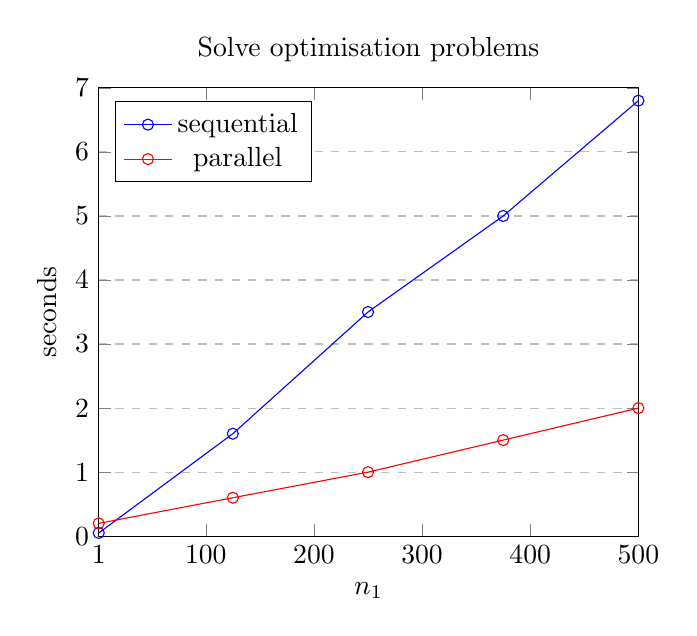
\begin{tikzpicture}
        \begin{axis}[
          title={Solve optimisation problems},
          xlabel={\(n_1\)},
          ylabel={seconds},
          xmin=1, xmax=500,
          ymin=0, ymax=7,
          xtick={1,100,200,300,400,500},
          ytick={0, 1, 2, 3, 4, 5, 6, 7},
          legend pos=north west,
          ymajorgrids=true,
          grid style=dashed,
          ]
          \addplot[color=blue, mark=o] coordinates {
            (1,0.05)(125,1.6)(250,3.5)(375,5)(500,6.8)
          };
          \addlegendentry{sequential}
          \addplot[color=red, mark=o] coordinates {
            (1,0.2)(125,0.6)(250,1)(375,1.5)(500,2)
          };
          \addlegendentry{parallel}          
        \end{axis}
      \end{tikzpicture}
    \end{minipage}\hfill
    \begin{minipage}[t]{.4\textwidth}
      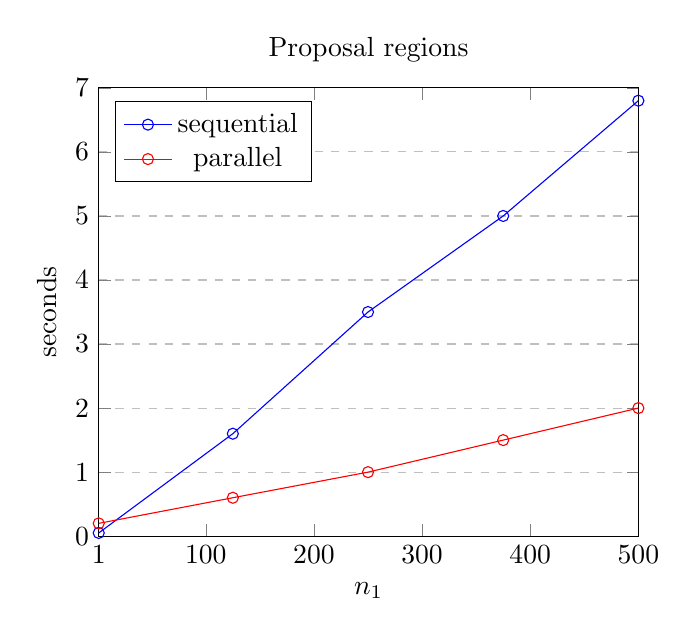
\begin{tikzpicture}
        \begin{axis}[
          title={Proposal regions},
          xlabel={\(n_1\)},
          ylabel={seconds},
          xmin=1, xmax=500,
          ymin=0, ymax=7,
          xtick={1,100,200,300,400,500},
          ytick={0, 1, 2, 3, 4, 5, 6, 7},
          legend pos=north west,
          ymajorgrids=true,
          grid style=dashed,
          ]
          \addplot[color=blue, mark=o] coordinates {
            (1,0.05)(125,1.6)(250,3.5)(375,5)(500,6.8)
          };
          \addlegendentry{sequential}
          \addplot[color=red, mark=o] coordinates {
            (1,0.2)(125,0.6)(250,1)(375,1.5)(500,2)
          };
          \addlegendentry{parallel}          
        \end{axis}
      \end{tikzpicture}
    \end{minipage}\hfill
    \begin{minipage}[t]{.4\textwidth}
      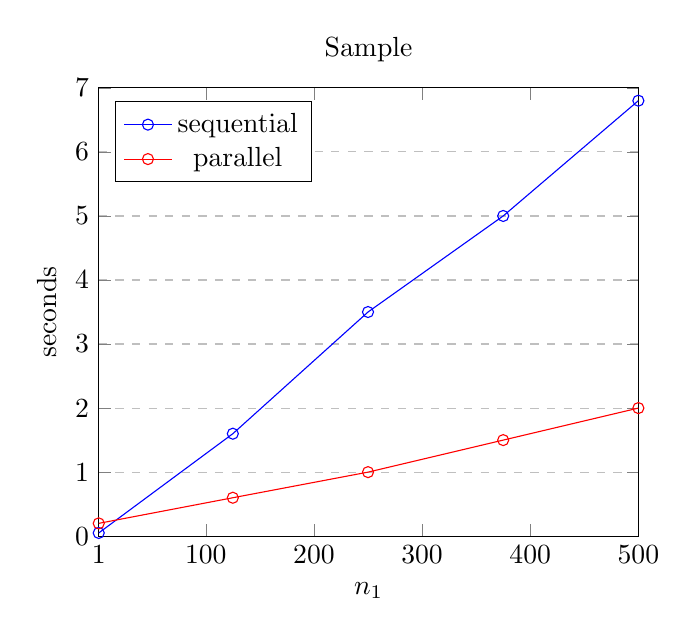
\begin{tikzpicture}
        \begin{axis}[
          title={Sample},
          xlabel={\(n_1\)},
          ylabel={seconds},
          xmin=1, xmax=500,
          ymin=0, ymax=7,
          xtick={1,100,200,300,400,500},
          ytick={0, 1, 2, 3, 4, 5, 6, 7},
          legend pos=north west,
          ymajorgrids=true,
          grid style=dashed,
          ]
          \addplot[color=blue, mark=o] coordinates {
            (1,0.05)(125,1.6)(250,3.5)(375,5)(500,6.8)
          };
          \addlegendentry{sequential}
          \addplot[color=red, mark=o] coordinates {
            (1,0.2)(125,0.6)(250,1)(375,1.5)(500,2)
          };
          \addlegendentry{parallel}          
        \end{axis}
      \end{tikzpicture}
    \end{minipage}\hfill
    \begin{minipage}[t]{.4\textwidth}
      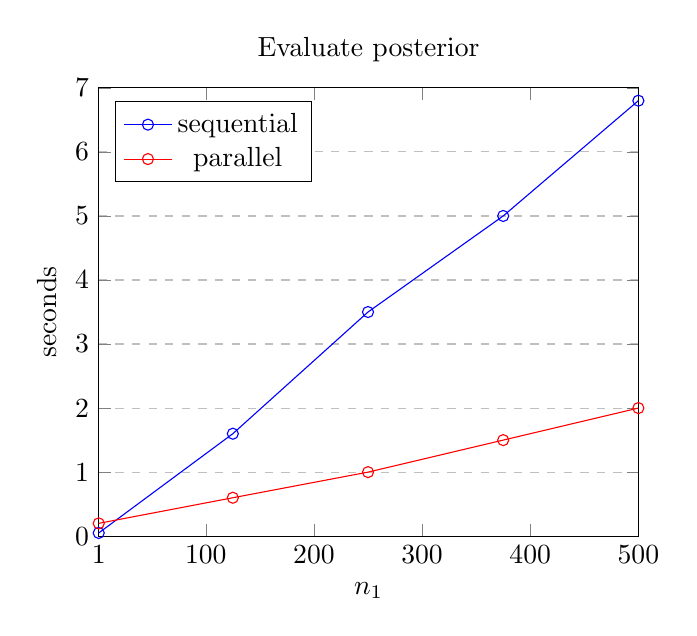
\begin{tikzpicture}
        \begin{axis}[
          title={Evaluate posterior},
          xlabel={\(n_1\)},
          ylabel={seconds},
          xmin=1, xmax=500,
          ymin=0, ymax=7,
          xtick={1,100,200,300,400,500},
          ytick={0, 1, 2, 3, 4, 5, 6, 7},
          legend pos=north west,
          ymajorgrids=true,
          grid style=dashed,
          ]
          \addplot[color=blue, mark=o] coordinates {
            (1,0.05)(125,1.6)(250,3.5)(375,5)(500,6.8)
          };
          \addlegendentry{sequential}
          \addplot[color=red, mark=o] coordinates {
            (1,0.2)(125,0.6)(250,1)(375,1.5)(500,2)
          };
          \addlegendentry{parallel}          
        \end{axis}
      \end{tikzpicture}
    \end{minipage}\hfill
    \caption[Execution time exploiting parallelisation]{In the first
      line, we compare the parallel and sequential execution of the
      training part and at the second line the inference part. At the
      left figure, we measure the execution time for sampling \(n_2=50\)
      points per region. At the right figure we measure the execution
      time for evaluating the posterior at a batch of \(50\) points.}
      \label{fig:exec_parallel}
\end{figure}